\documentclass[11pt,a4paper,twoside]{bayesxreport}

\usepackage{amsfonts}
\usepackage[dvips]{graphicx}
\usepackage[dvips]{epsfig}
\usepackage{fancyhdr}

%\usepackage{showkeys}
%\usepackage{showidx}

\usepackage{rotating}
\usepackage{shortvrb}
\usepackage{multicol}
\usepackage{xr}

\usepackage[ps2pdf]{thumbpdf}
\usepackage[ps2pdf]{hyperref}
\hypersetup{
%    pdffitwindow=true,
    pdfstartview=FitB,
    pdftitle={BayesX Reference Manual},
    pdfauthor={Andreas Brezger, Thomas Kneib and Stefan Lang with contributions
    by Christiane Belitz, Eva-Maria Fronk, Andrea Hennerfeind,
    Petra Kragler, Manuela Hummel and Leyre Osuna Echavarr\'{\i}a},
    colorlinks=true,
    linkcolor=blue,
    pdfpagemode=UseOutlines,
    bookmarksopen=true,
    bookmarksnumbered=true,
    pdfstartpage={1},
    hyperindex=true
    }

\sloppy
\parindent0em
\parskip0.3em
\topmargin -0.3cm
\textheight24cm
\textwidth16.5cm
\headheight0.5cm
\oddsidemargin-0.4cm
\evensidemargin-0.4cm

 \fancyhead[RO,LE]{\thepage}
 \fancyhead[C]{}
 \fancyhead[LO]{\nouppercase\rightmark}
 \fancyhead[RE]{\nouppercase\leftmark}
 \fancyfoot[RO,LE]{}
 \fancyfoot[C]{\small\today} %Am ende raus!!!
 \fancyfoot[LO,RE]{}
 \fancyfoot[C]{}

 \renewcommand{\headrulewidth}{.4pt}
 \renewcommand{\footrulewidth}{0pt} %Am Ende 0 !!!

\pagestyle{fancy}


\renewcommand{\descriptionlabel}[1]{\hspace\labelsep\sc #1}

\def \re {{\bf R}}
\def \beq {\begin{equation}}
\def \eeq {\end{equation}}
\def \bdis {\begin{displaymath}}
\def \edis {\end{displaymath}}
\def \ds {\displaystyle}

\def \mbeta {\mbox{\boldmath $\beta$}}
\def \mtheta {\mbox{\boldmath $\theta$}}
\def \hatmbeta {\mbox{\boldmath $\hat\beta$}}
\def \eps {\epsilon}
\def \meps {\mbox{\boldmath $\epsilon$}}
\def \mmu {\mbox{\boldmath $\mu$}}
\def \mnu {\mbox{\boldmath $\nu$}}
\def \mSigma {\mbox{\boldmath $\Sigma$}}
\def \mGamma {\mbox{\boldmath $\Gamma$}}
\def \msigma {\mbox{\boldmath $\sigma$}}
\def \mPhi {\mbox{\boldmath $\Phi$}}

\newcommand{\N}{\mbox{N}}
\newcommand{\Var}{\mbox{Var}}
\newcommand{\E}{\mbox{E}}

\newcommand{\X}{\mbox{\boldmath $X$}}
\newcommand{\x}{\mbox{\boldmath $x$}}
\newcommand{\Z}{\mbox{\boldmath $Z$}}
\newcommand{\z}{\mbox{\boldmath $z$}}
\newcommand{\mb}{\mbox{\boldmath $b$}}
\newcommand{\Fx}{\mbox{\scriptsize \boldmath $x$}}
\newcommand{\I}{\mbox{\boldmath $I$}}
\newcommand{\Y}{\mbox{\boldmath $Y$}}
\newcommand{\y}{\mbox{\boldmath $y$}}
\newcommand{\mS}{\mbox{\boldmath $S$}}
\newcommand{\T}{\mbox{\boldmath $T$}}
\newcommand{\K}{\mbox{\boldmath $K$}}
\newcommand{\kt}{\mbox{\boldmath $t$}}
\newcommand{\U}{\mbox{\boldmath $U$}}
\newcommand{\fu}{\mbox{\boldmath $u$}}
\newcommand{\ba}{\mbox{\boldmath $\alpha$}}
\newcommand{\bb}{\mbox{\boldmath $\beta$}}

\renewcommand{\chaptername}{Chapter}

\newcommand{\subheader}[1]{\textsf{\textbf{{\large #1}}}}

\newenvironment{stanza}[2]{\subheader{#1} \begin{itemize} \item[]#2}{\end{itemize}}

 \externaldocument{manual_star}
 \externaldocument{manual_tutorials}

\makeindex

\setcounter{secnumdepth}{3}

\begin{document}
\MakeShortVerb{\#}


\usepackage{amsfonts}
\usepackage[dvips]{graphicx}
\usepackage[dvips]{epsfig}
\usepackage{fancyhdr}
\usepackage{dsfont}
\usepackage{amsmath}
\usepackage{dsfont}
\usepackage{amssymb}

%\usepackage{showkeys}
%\usepackage{showidx}

\usepackage{rotating}
\usepackage{shortvrb}
\usepackage{multicol}
\usepackage{longtable}
\usepackage{xr}

\usepackage[ps2pdf]{thumbpdf}
\usepackage[ps2pdf]{hyperref}

\input{prepictex}
\input{pictexwd}
\input{postpictex}

\hypersetup{
%    pdffitwindow=true,
    pdfstartview=FitB,
    pdftitle={BayesX Manuals},
    pdfauthor={Christiane Belitz, Andreas Brezger, Thomas Kneib, Stefan Lang and Nikolaus Umlauf},
    colorlinks=true,
    linkcolor=blue,
    pdfpagemode=UseOutlines,
    bookmarksopen=true,
    bookmarksnumbered=true,
    pdfstartpage={1},
    hyperindex=true
    }

\usepackage[dcu]{harvard}

\sloppy
\parindent0em
\parskip0.3em
\topmargin -0.3cm \textheight24cm \textwidth16.5cm \headheight0.5cm \oddsidemargin-0.4cm \evensidemargin-0.4cm

 \fancyhead[RO,LE]{\thepage}
 \fancyhead[C]{}
 \fancyhead[LO]{\nouppercase\rightmark}
 \fancyhead[RE]{\nouppercase\leftmark}
 \fancyfoot[RO,LE]{}
 \fancyfoot[C]{\small\today} %Am ende raus!!!
 \fancyfoot[LO,RE]{}
 \fancyfoot[C]{}

 \renewcommand{\headrulewidth}{.4pt}
 \renewcommand{\footrulewidth}{0pt} %Am Ende 0 !!!

\pagestyle{fancy}


\renewcommand{\descriptionlabel}[1]{\hspace\labelsep\sc #1}

 \newcommand{\Cov}{\mbox{Cov}}
 \newcommand{\diag}{\mbox{diag}}
 \newcommand{\trace}{\mbox{trace}}
 \newcommand{\df}{\mbox{df}}

\def \re {{\bf R}}
\def \beq {\begin{equation}}
\def \eeq {\end{equation}}
\def \bdis {\begin{displaymath}}
\def \edis {\end{displaymath}}
\def \ds {\displaystyle}

\def \mbeta {\mbox{\boldmath $\beta$}}
\def \mtheta {\mbox{\boldmath $\theta$}}
\def \hatmbeta {\mbox{\boldmath $\hat\beta$}}
\def \eps {\epsilon}
\def \meps {\mbox{\boldmath $\epsilon$}}
\def \mmu {\mbox{\boldmath $\mu$}}
\def \mnu {\mbox{\boldmath $\nu$}}
\def \mSigma {\mbox{\boldmath $\Sigma$}}
\def \mGamma {\mbox{\boldmath $\Gamma$}}
\def \msigma {\mbox{\boldmath $\sigma$}}
\def \mPhi {\mbox{\boldmath $\Phi$}}
\def \Sigmavec {\mbox{\boldmath $\Sigma$}}
\def \sigmavec {\mbox{\boldmath $\sigma$}}
\def \nuvec {\mbox{\boldmath $\nu$}}
\def \tauvec {\mbox{\boldmath $\tau$}}




\newcommand{\N}{\mbox{N}}
\newcommand{\Var}{\mbox{Var}}
\newcommand{\E}{\mbox{E}}

\newcommand{\X}{\mbox{\boldmath $X$}}
\newcommand{\x}{\xvec}
\newcommand{\Z}{\mbox{\boldmath $Z$}}
\newcommand{\z}{\mbox{\boldmath $z$}}
\newcommand{\mb}{\mbox{\boldmath $b$}}
\newcommand{\Fx}{\mbox{\scriptsize \boldmath $x$}}
\newcommand{\I}{\mbox{\boldmath $I$}}
\newcommand{\Y}{\mbox{\boldmath $Y$}}
\newcommand{\y}{\mbox{\boldmath $y$}}
\newcommand{\mS}{\mbox{\boldmath $S$}}
\newcommand{\T}{\mbox{\boldmath $T$}}
\newcommand{\K}{\mbox{\boldmath $K$}}
\newcommand{\kt}{\mbox{\boldmath $t$}}
\newcommand{\U}{\mbox{\boldmath $U$}}
\newcommand{\fu}{\mbox{\boldmath $u$}}
\newcommand{\ba}{\mbox{\boldmath $\alpha$}}
\newcommand{\bb}{\mbox{\boldmath $\beta$}}

\def \Mvec {\vec{M}}
\def \Kvec {\vec{K}}
\def \mM {\vec{M}}
\def \Pvec {\vec{P}}
\def \Svec {\vec{S}}
\def \deltavec {\vec{\delta}}
\def \lambdavec {\boldsymbol{\lambda}}
\def \Lambdavec {\boldsymbol{\Lambda}}
\def \betavec {\boldsymbol{\beta}}
\def \etavec {\boldsymbol{\eta}}
\def \gammavec {\boldsymbol{\gamma}}
\def \Gammavec {\boldsymbol{\Gamma}}
\def \Omegavec {\boldsymbol{\Omega}}
\def \muvec {\boldsymbol{\mu}}
\def \kappavec {\boldsymbol{\kappa}}
\def \nuvec {\boldsymbol{\nu}}
\def \pivec {\vec{\pi}}
\def \thetavec {\vec{\theta}}
\def \varthetavec{\vec{\vartheta}}
\def \varepsilonvec {\boldsymbol{\varepsilon}}
\def \zetavec {\vec{\zeta}}
\def \Sigmavec {\boldsymbol{\Sigma}}
\def \Thetavec {\boldsymbol{\theta}}

\def \dvec {\mathbf{d}}
\def \fvec {\mathbf{f}}
\def \fhatvec {\mathbf{\hat{f}}}
\def \svec {\mathbf{s}}
\def \wvec {\mathbf{w}}
\def \xvec {\mathbf{x}}
\def \yvec {\mathbf{y}}
\def \uvec {\mathbf{u}}
\def \avec {\mathbf{a}}
\def \zvec {\mathbf{z}}
\def \bvec {\mathbf{b}}
\def \tvec {\mathbf{t}}
\def \mvec {\mathbf{m}}
\def \cvec {\mathbf{c}}

\def \ds {\displaystyle}

\def \Gvec {\mathbf{G}}
\def \Rvec {\mathbf{R}}
\def \Avec {\mathbf{A}}
\def \Bvec {\mathbf{B}}
\def \Cvec {\mathbf{C}}
\def \Dvec {\mathbf{D}}
\def \Fvec {\mathbf{F}}
\def \Kvec {\mathbf{K}}
\def \Hvec {\mathbf{H}}
\def \Ivec {\mathbf{I}}
\def \Lvec {\mathbf{L}}
\def \Uvec {\mathbf{U}}
\def \Wvec {\mathbf{W}}
\def \Yvec {\mathbf{Y}}
\def \Zvec {\mathbf{Z}}
\def \svec {\mathbf{s}}
\def \Cvec {\mathbf{C}}
\def \dvec {\mathbf{d}}
\def \Avec {\mathbf{A}}
\def \Pvec {\mathbf{P}}
\def \Vvec {\mathbf{V}}
\def \xivec {\mathbf{x_i}}
\def \xjvec {\mathbf{x_j}}
\def \betavecr {\vec{\beta_r}}
\def \betavec {\boldsymbol{\beta}}
\def \betadach {\hat{\vec{\beta}}}
\def \betadachr {\vec{\hat{\beta}_r}}
\def \betaschl {\vec{\tilde{\beta}}}
\def \betaschlr {\vec{\tilde{\beta}_r}}
\def \sschlr {\vec{\tilde{s}_r}}
\def \Aschlr {\vec{\tilde{A}_r}}
\def \Adach {\vec{\hat{A}}}
\def \Avecr {\vec{A}_r}
\def \Adachr {\vec{\hat{A}_r}}
\def \Fdach {\vec{\hat{F}}}
\def \Vdach {\vec{\hat{V}}}
\def \Aschl {\vec{\tilde{A}}}
\def \Xvec {\mathbf{X}}

\def \nullvec {\boldsymbol{0}}

\def \hvec {\vec{h}}
\def \vvec {\vec{v}}
\def \wvec {\vec{w}}
\def \x1vec {\vec{x_1}}
\def \xnvec {\vec{x_n}}

\def \Kmat {\mathbf{K}}
\def \Kmatj {\mathbf{K}_j}
\def \Xmat {\mathbf{X}}
\def \Vmat {\mathbf{V}}
\def \Smat {\mathbf{S}}


\def \dsR {\text{$\mathds{R}$}}
 \DeclareMathOperator{\B}{B}

\def \einsvec {\boldsymbol{1}}

\newcommand{\subheader}[1]{\textsf{\textbf{{\large #1}}}}

\newenvironment{stanza}[2]{\subheader{#1} \begin{itemize} \item[]#2}{\end{itemize}}


\newcommand{\preface}[1]{
\thispagestyle{empty}

\begin{center}
{\bf \em \huge BayesX}

\vspace{0.5cm}

{\em \large Software for Bayesian Inference in Structured Additive Regression Models}

\vspace{0.5cm}

{\em Version 2.1}

\vspace{0.5cm}

\begin{figure}[h]
\begin{center}
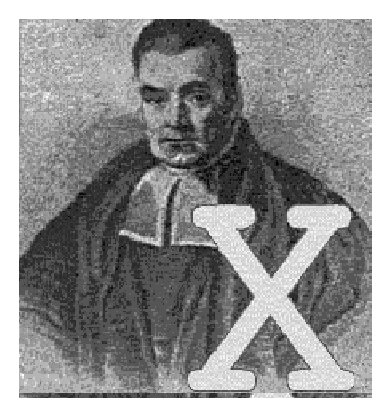
\includegraphics[scale=1.2]{grafiken/bayesicon.eps}
\end{center}
\end{figure}

\vfill

{\bf\sffamily \huge #1}

\vfill

\end{center}

{\em Developed by}

Christiane Belitz\\
Andreas Brezger\\
Thomas Kneib (University of G{\"o}ttingen)\\
Stefan Lang (University of Innsbruck) \\
Nikolaus Umlauf (University of Innsbruck) \\

\vspace{2ex}

{\em With contributions by}

\vspace{-1.5ex}

\begin{multicols}{2}
Daniel Adler
Eva-Maria Fronk\\
Felix Heinzl\\
Andrea Hennerfeind\\
Manuela Hummel\\
Alexander Jerak\\
Susanne Konrath\\
Petra Kragler\\
Cornelia Oberhauser\\
Leyre Est\'{\i}baliz Osuna Echavarr\'{\i}a\\
Daniel Saban\'{e}s Bov\'{e} \\
Achim Zeileis
\end{multicols}

{\em Supported by}

Ludwig Fahrmeir (mentally)\\
Leo Held (mentally)\\
German Research Foundation (DFG)

\newpage

\subsection*{Acknowledgements}

The development of {\em BayesX} has been supported by grants from the German Research Foundation (DFG), Collaborative
Research Center 386 ``Statistical Analysis of Discrete Structures''.

Special thanks go to (in alphabetical order of first names):

{\em Dieter Gollnow} for computing and providing the map of Munich (a really hard job); \\
{\em Leo Held} for advertising the program; \\
{\em Ludwig Fahrmeir} for his patience with finishing the program and for carefully
reading and correcting the  manual; \\
{\em Ngianga-Bakwin Kandala} for being the first user of the program (a really hard job); \\
{\em Samson Babatunde Adebayo} for carefully reading and correcting the manual; \\
{\em Ursula Becker} for carefully reading and correcting the manual;

\subsection*{Licensing agreement}

This program is free software; you can redistribute it and/or
modify it under the terms of the GNU General Public License
as published by the Free Software Foundation; either version 2
of the License, or (at your option) any later version.

This program is distributed in the hope that it will be useful,
but WITHOUT ANY WARRANTY; without even the implied warranty of
MERCHANTABILITY or FITNESS FOR A PARTICULAR PURPOSE.  See the
GNU General Public License for more details.

You should have received a copy of the GNU General Public License
along with this program; if not, write to the Free Software
Foundation, Inc., 51 Franklin Street, Fifth Floor, Boston, MA  02110-1301, USA.



\vspace{0.5cm}

{\em BayesX} is available at { \href{http://www.bayesx.org}{http://www.bayesx.org}}}


\chapter{What is BayesX?}

{\em BayesX} is a software tool for performing complex Bayesian
inference. The main features of {\em BayesX} are:
\begin{itemize}
\item {\bf Bayesian semiparametric regression based on MCMC simulation techniques} \\
{\em BayesX} provides a powerful regression tool for analyzing
regression and survival models with {\em structured additive
predictor} (STAR). STAR models cover a number of well known model
classes as special cases, e.g. {\em generalized additive models},
{\em generalized additive mixed models}, {\em geoadditive models},
{\em dynamic models}, {\em varying coefficient models}, and {\em
geographically weighted regression}. {\em BayesX} is able to
estimate nonlinear effects of continuous covariates, trends and
flexible seasonal patterns of time scales, correlated and/or
uncorrelated spatial effects (of geographical data) and
unstructured i.i.d. Gaussian effects of unordered group
indicators. The regression tool  supports the most common
distributions for the response variable. Supported distributions
for univariate responses are Gaussian, binomial, Poisson, negative
binomial and gamma. For multicategorial responses, both
multinomial logit or probit models for ordered categories of the
responses as well as cumulative threshold models for unordered
categories may be estimated. Recently complex models for
continuous time survival analysis based on the Cox model have been
added. At least some basic knowledge about Bayesian inference with
MCMC techniques is strongly recommended if you are interested in
using this tool. Details can be found in \autoref{star} and
\autoref{bayesreg}.
\item {\bf Inference for STAR models based on methodology for mixed models} \\
{\em BayesX} provides a second regression tool for estimating STAR
models with comparable functionality as the first tool based on
MCMC. This tool represents STAR models as {\em variance components
mixed models}. Inference is then based on estimation procedures
for mixed models, particularly {\em restricted maximum likelihood}
(REML). From a Bayesian perspective this yields empirical Bayes or
posterior mode estimates. Details can be found in \autoref{star}
and \autoref{remlreg}.
\item {\bf Model selection for Gaussian and non-Gaussian dag's} \\
This tool estimates Gaussian and non-Gaussian directed acyclical
graphs (dag) via reversible jump MCMC. Details are given in
\autoref{dag}
\item {\bf Handling and manipulation of data sets} \\
{\em BayesX} provides a growing number of functions for handling
and manipulating data sets, e.g. for reading ASCII data sets,
creating new variables, obtaining summary statistics etc. Details
are given in \autoref{datasetobj}.
\item {\bf Handling and manipulation of geographical maps} \\
{\em BayesX} is able to manipulate and draw geographical maps. The
regions of the map may be colored according to some numerical
characteristics. For details compare \autoref{map} and
\autoref{graphobj}.
\item {\bf Visualizing data} \\
{\em BayesX} provides functions for drawing scatter plots and
geographical maps. A number of additional options are provided to
customize the graphs according to the personal needs of the user.
Details can be found in \autoref{graphobj}.
\end{itemize}

\vspace{0.5cm} {\bf Recommendations for further reading}

\vspace{0.2cm} If you are interested in using {\em BayesX} it is
not necessary to read the complete manual. \autoref{recomm}
provides a guideline for reading this manual and other sources
depending on your purpose and background. In any case, you should
read \autoref{availableversions}-\autoref{generalusage} of
\autoref{gettingstarted} to make yourself familiar with {\em
BayesX}.


\begin{table}[ht] \footnotesize
\begin{center}
\begin{tabular}{ |p{7cm}|p{8.5cm}|}
\hline
{\bf Intended use and background} & {\bf Guideline} \\
\hline\hline Bayesian semiparametric regression based on MCMC
simulation techniques. No experience with MCMC techniques. & Read
first an introductory text about MCMC. A nice introduction is
given e.g. in Green (2001). Read \autoref{star} to make yourself
familiar with STAR regression models.
Proceed then with the tutorial like \autoref{zambiaanalysis} of \autoref{bayesreg}. \\
\hline Bayesian semiparametric regression based on MCMC simulation
techniques. At least a basic knowledge about MCMC techniques
exists. & Read \autoref{star} to make yourself familiar
with STAR regression models. Proceed then with the tutorial like \autoref{zambiaanalysis} of \autoref{bayesreg}. \\
\hline Semiparametric regression based on mixed model methodology.
& Read \autoref{star} to make yourself familiar with STAR
regression models. Proceed then with the tutorial like
\autoref{remlregzambianalysis} of \autoref{remlreg}. \\
\hline Model selection for dag's. No experience with reversible
jump MCMC. & Read first an introductory text about reversible jump
MCMC. A nice introduction is
given e.g. in Green (2001). Proceed with \autoref{dag}. \\
\hline
Draw and color geographical maps & Read \autoref{map} and \autoref{graphdrawmap} of \autoref{graphobj}. \\
\hline
\end{tabular}
{\em \caption {\label{recomm} Recommendations for further
reading}}
\end{center}
\end{table}

\subsubsection*{References}

\begin{description}
\item[Green, P.J. (2001):] A Primer in Markov Chain Monte Carlo. In: Barndorff-Nielsen, O.E.,
Cox, D.R. and Kl{\"u}ppelberg, C. (eds.), {\em Complex Stochastic
Systems}. Chapman and Hall, London, 1-62.
\end{description}


\chapter{Getting started}
\label{gettingstarted}

This chapter provides some useful information for first-time users
of {\em BayesX}: Which versions of BayesX are currently available
(\autoref{availableversions}), how is BayesX installed
(\autoref{installbayesx}), what types of manuals exist
(\autoref{bayesxmanuals}), and how is the graphical user interface
organized (\autoref{bayesxwindows}). Section \ref{generalusage}
describes the general usage of {\em BayesX} and the structure of
{\em BayesX} syntax. The final section contains a description of
three data sets that will be used for demonstrating purposes in
the later chapters.

\section{Available versions of BayesX}
\label{availableversions} \index{Java based version} \index{Non-Java
based version} \index{Versions} \index{Versions!Java based}
\index{Versions!Non-Java based}

In its current form, {\em BayesX} runs only under the various
versions of the Windows operating system (e.g. Windows 95, 98,
2000, NT, XP). The graphical user interface and the visualisation
tools are implemented in Java, while the computerintensive parts
of the program have been implemented in C++. The current version
of {\em BayesX} can be downloaded from
\href{http://www.stat.uni-muenchen.de/~bayesx}
{http://www.stat.uni-muenchen.de/\~{}bayesx}.

Up to version 1.3, {\em BayesX} has been distributed in two
versions, the {\em Java based version} described above and a {\em
non-Java based version}, which was written completely in C++.
Since the Java based version has additional features, the non-Java
based version is no longer supported.

\section{Installing BayesX}\label{installbayesx}
\index{Installation} \index{Installation directories}

After you have downloaded the file #installBayesX.exe# from the
{\em BayesX} homepage, proceed by executing this file. The
installation process is quite simple and comparable to most
standard installations. The installation routine will request all
necessary information.

When {\em BayesX} has been installed successfully, it can be
started using the {\em Windows Start} button or the icon created
on the desktop (depending on your specifications during the
installation process). The installation directory contains the
five subdirectories #doc#, #examples#, #output#, #sfunctions# and
#temp#. The #doc# directory contains the program documentation,
i.e. the three {\em BayesX} manuals (see the following
subsection). The #examples# directory contains the three data
sets, #credit.raw#, #rents.raw# and #zambia.raw#, which will be
used for demonstrating purposes throughout the manual. A detailed
description of these data sets is given in
\autoref{datadescription}. The #examples# directory also contains
some tutorial programs that illustrate the usage of {\em BayesX},
see the tutorials manual. The #output# directory is the default
directory for program output stored in files. Of course, the
output window can be redefined by the user, compare
\autoref{bayesregglobopt} and \autoref{remlregglobopt}. The
#sfunctions# directory contains some R and S-plus functions for
visualizing estimation results obtained with {\em bayesreg
objects} or {\em remlreg objects}, see \autoref{splus} for a
detailed description of these functions. Note, however, that the
current {\em BayesX} version has its own graphics capabilities,
see \autoref{graphobj} and \autoref{visualization} for details.
Finally, temporary files created when estimating regression models
will be stored in the #temp# directory. Usually you will never use
this directory.

The subdirectories and their content are briefly summarized in
\autoref{dirtable}.

\begin{table}[ht]
\begin{center}
\begin{tabular}{|l|l|}
\hline
Directory & Content \\
\hline
#doc# & the {\em BayesX} manuals \\
#examples# & data set examples and tutorial programs \\
#output# & default directory for estimation output \\
#sfunctions# & R and S-plus functions for visualizing output \\
#temp# & temporary files \\
\hline
\end{tabular}
{\em\caption{ \label{dirtable} Subdirectories of the installation
directory and their content.}}
\end{center}
\end{table}

\section{Manuals}\label{bayesxmanuals}
\index{Manuals}

{\em BayesX} is shipped with three different manuals. The
reference manual (i.e. the manual you are just reading) gives
detailed information on the general usage of BayesX, the syntax of
{\em BayesX} commands and the different objects used by {\em
BayesX}. The methodology manual provides background information on
the statistical methodology that is implemented in {\em BayesX}.
In this manual you will also find more references on the
methodological background. The tutorial manual is intended to make
new users familiar with the usage of {\em BayesX} by demonstrating
examples. It contains two self-contained tutorials, describing how
to perform semiparametric regression analyses using {\em BayesX}.
The manuals are also available from the help menu and can be found
in the #doc# directory (a subdirectory of the installation
directory).

\section{Windows and buttons in BayesX}\label{bayesxwindows}
\index{Windows}

After starting {\em BayesX} you will see a main window with a menu
bar and four additional subwindows. The four windows are the {\em
command window}, the {\em output window}, the {\em review window}
and the {\em object browser}. The purpose of these windows is
described in the following four subsections. Below the menu bar
there is a menu bar containing the buttons BREAK, PAUSE and
SUPPRESS OUTPUT, and the priority menu. Their functionality is
described in subsection \ref{buttons} and \ref{prioritymenu}.

\subsection{The command window}
\index{Command window} \index{Windows!Command}

Allmost all {\em BayesX} commands are entered and executed in the
{\em command window}. By default, a command will be executed if
you press the return key. You can change this default delimiter
using the #delimiter# command, see \autoref{delimiter}.

\subsection{The output window}
\index{Output window} \index{Windows!Output}

In the {\em output window}, all commands entered in the {\em
command window} or executed through a batch file (see
\autoref{batch}) are printed together with the program output.

\index{Saving the output} The content of the {\em output window} can
be saved and processed with your favorite text editor. For saving
the output, enter the {\em file menu} and click on {\em Save output}
or {\em Save output as}. The file save dialog will allow you to
choose between two different file formats. The default is the
rich-text format but it is also possible to store the {\em output
window} in plain ASCII format. This, however, has the disadvantage
that all text highlights (for example bold letters) will disappear
in the saved file.

The {\em file menu} also allows to clear the {\em output window}
(i.e. delete the content of the window) or to open an already
existing file.

Depending on the screen resolution of your computer, letters
appearing in the {\em output window} may be very small or too
large. The font size can be varied in the {\em preferences menu}.

\subsection{The review window}
\index{Review window} \index{Windows!Review}

In many cases, subsequent commands change only slightly. The {\em
review window} gives you convenient access to the last 100 past
commands entered during a session. Double click on one of these
past commands and it is automatically copied to the {\em command
window}, where it can be modified and / or executed again.

\subsection{The object browser}
\index{Object browser}

{\em BayesX} is object oriented, i.e. different types of objects
are used to store data, estimate regression models, etc. The {\em
object browser} provides an overview of the objects currently
defined and about their contents. The {\em object browser} window
is split into two parts. The left part displays the different
object types currently supported by {\em BayesX} ({\em dataset
objects}, {\em bayesreg objects}, {\em remlreg objects}, {\em map
objects}, {\em dag objects} and {\em graph objects})s. By clicking
on one of the object types, the names of all objects of this type
will appear in the right panel of the {\em object browser}. Double
clicking on one of the names gives a visualization of the object
and / or a short summary in the {\em output window}, depending on
the object type. Double clicking on {\em dataset objects}, for
example, will open a spreadsheet where the variables and the
observations of the data set can be inspected. Clicking on {\em
map objects} opens a window that contains a graphical
representation of the map.

\subsection{BREAK, PAUSE and SUPPRESS OUTPUT button}
\label{buttons} \index{PAUSE button} \index{BREAK button}
\index{SUPPRESS OUTPUT button} \index{Buttons} \index{Buttons!PAUSE}
\index{Buttons!BREAK} \index{Buttons!SUPPRESS OUTPUT}

The {\em BayesX} button panel contains the BREAK button, the PAUSE
button and the SUPPRESS OUTPUT button. The purpose of the BREAK
button is to interrupt the process that is currently executed
(this may take some time). Clicking on the PAUSE button interrupts
the current process temporarily until the button is pressed again.
If a process is paused, the button caption PAUSE is replaced by
CONTINUE, indicating that a second click on the button will
continue the current process. Pausing a current process will
increase the execution speed of other programs currently running
on your computer. Clicking the SUPPRESS OUTPUT button suppresses
printing of output in the {\em output window}. The button caption
changes to SHOW OUTPUT to indicate that an additional click on the
button will cause the program to print the output again.
Suppressing the output increases the execution speed of {\em
BayesX} and saves memory. Note, that you can store your output in
a log-file even if printing of the output is suppressed (see
\autoref{logfile}).

\subsection{Priority menu}
\label{prioritymenu} \index{Priority menu}

When running extensive computations, it may be desirable to reduce
the priority of BayesX since otherwise all further programs may be
executed very slowly. The priority menu allows you to change the
priority of your computations from within BayesX. Usually there
should be no need to increase the priority (although it is
possible). To pause the current computations use the PAUSE button.

\section{General usage of BayesX}
\label{generalusage}

\subsection{Creating objects}
\label{createobject} \index{Objects} \index{Objects!Create}

{\em BayesX} is implemented in an object oriented way, although
the object oriented concept does not go too far, i.e. inheritance
or other concepts of object oriented programming languages such as
S or C++ are not supported. As a consequence, the first thing to
do during a session, is to create some objects. Currently, six
different object types are available: {\em dataset objects}, {\em
bayesreg objects}, {\em remlreg objects}, {\em map objects}, {\em
dag objects} and {\em graph objects}. {\em Dataset objects} are
used to store, handle, and manipulate data sets, see
\autoref{datasetobj} for details. {\em Map objects} are used to
handle geographical information and are covered in more detail in
\autoref{map}. The main purpose of {\em map objects} is to serve
as auxiliary objects for {\em bayesreg objects} or {\em remlreg
objects} when estimating spatial effects. {\em Graph objects} are
used to visualize data (e.g. to create scatterplots or to color
geographical maps according to some numerical characteristics),
see \autoref{graphobj} for details. The most important object
types are {\em bayesreg objects} and {\em remlreg objects}. These
objects are used to estimate Bayesian semiparametric regression
models based on either Markov Chain Monte Carlo simulation
techniques ({\em bayesreg objects}) or a mixed model
representation of the regression model ({\em remlreg objects}).
See \autoref{bayesreg} for a detailed description of {\em bayesreg
objects} and \autoref{remlreg} for a detailed description of {\em
remlreg objects}. {\em Dag objects} are used to estimate Gaussian
or non-Gaussian DAGs (direct acyclic graphs) based on reversible
jump MCMC simulation techniques (see \autoref{dag} for details).

The syntax for creating a new object is:

#># {\em objecttype objectname}

To create for example a {\em dataset object} with name #mydata#, simply type:

#> dataset mydata#

Note that some restrictions are imposed on the names of objects,
i.e. not all object names are allowed. For example, object names
have to begin with an uppercase or lowercase letter rather than a
number. Section \ref{varnames} discusses valid variable names but
the same rules apply also to object names.

\subsection{Applying methods to previously defined objects}

When an object has been created successfully, you can apply methods
to that particular object. For instance, {\em dataset objects} may
be used to read data stored in an ASCII file using method #infile#,
to create new variables using method #generate#, to modify existing
variables using method #replace# and so on. The syntax for applying
methods to the objects is similar for all methods and independent of
the particular object type. The general syntax is: \index{General
syntax} \index{Syntax}

#># {\em objectname.methodname} [{\em model}] [#weight# {\em varname}] [#if# {\em boolean expression}] [, {\em options}] \\
\hspace*{4.8cm} [#using# {\em usingtext}]

\autoref{syntaxtable} explains the syntax parts in more detail.


\begin{table}[ht]
 \centering
\begin{tabular}{|l|l|}
\hline
Syntax part & Description \\
\hline
{\em objectname} & the name of the object to apply the method to \\
{\em methodname} & the name of the method \\
{\em model} & a model specification (for example a regression model) \\
{\em #weight# varname} & specifies {\em varname} as weight variable \\
#if# {\em boolean expression} & indicates that the method should be applied only if a \\
& certain condition holds \\
, {\em options} & define (or modify) options for the method \\
#using# {\em usingtext} & indicates that another object or file is required to \\
& apply the particular method \\
\hline
\end{tabular}
{\em \caption{\label{syntaxtable}Parts of the general BayesX
syntax.}}
\end{table}

Note that $[\dots]$ indicates that this part of the syntax is
optional and may be omitted. Moreover for most methods only some
of the syntax parts above will be meaningful. The specification of
invalid syntax parts is not allowed and will cause an error
message.

We illustrate the concept with some simple methods of {\em dataset
objects}. Suppose that a {\em dataset object} with name #mydata#
has already been created and that some variables should be
created. First of all, we have to tell {\em BayesX} how many
observations we want to create. This can be done with the
 #set obs# command, see also \autoref{setobs}. For example

#> mydata.set obs = 1000#

indicates that the data set #mydata# should have 1000
observations. In this case, the {\em methodname} is #set# and the
{\em model} is #obs =# #1000#. Since no other syntax parts (for
example #if# statements) are meaningful for this method, they are
not allowed. For instance, specifying an additional weight
variable #x# by typing

#> mydata.set obs = 1000 weight x#

will cause the error message:

#ERROR: weight statement not allowed#

In a second step we can now create a new variable #X#, say, that
contains Gaussian (pseudo) random numbers with mean 2 and standard
deviation 0.5:

#> mydata.generate X = 2+0.5*normal()#

Here, #generate# is the {\em methodname} and #X = 2+0.5*normal()#
is the {\em model}. In this case the {\em model} consists of the
specification of the new variable name, followed by the equal sign
'#=#' and a mathematical expression for the new variable. Similar
as for the #set obs# command other syntax parts are not meaningful
and therefore not allowed. If the negative values of #X# should be
replaced with the constant 0, this can be achieved using the
#replace# command:

#> mydata.replace X = 0 if X < 0#

Obviously, the #if# statement is meaningful and is therefore
allowed, but not required.

\section{Description of data set examples}
\label{datadescription} \index{Data set examples}

This section describes three data sets used to illustrate many of
the features of {\em BayesX} in the following chapters as well as
in the tutorial manual. All data sets are stored columnwise in
plain ASCII-format. The first row of each data set contains the
variable names separated by blanks. Subsequent rows contain the
observations, one observation per row.

\subsection{Rents for flats}
\label{rentdata} \index{Rents for flats} \index{Data set
examples!Rents for flats}

According to the German rental law, owners of apartments or flats
can base an increase in the amount that they charge for rent on
'average rents' for flats comparable in type, size, equipment,
quality and location in a community. To provide information about
these 'average rents', most of the larger cities publish 'rental
guides', which can be based on regression analyses with rent as
the dependent variable. The file #rent94.raw# (stored in the
#examples# directory) is a subsample of data collected in 1994 for
the Munich rental guide. The variable of primary interest is the
monthly rent per square meter in German Marks. Covariates
characterizing the flat were constructed from almost 200 variables
out of a questionnaire answered by tenants of flats. The present
data set contains a small subset of these variables that are
sufficient for demonstration purposes (see \autoref{rentdatavar}).

In addition to the data set, the #examples# directory contains a
map of Munich in the file #munich.bnd#. This map will be useful
for visualizing effects of the location #L#. See \autoref{map} for
a description on how to incorporate geographical maps into {\em
BayesX}.

\begin{table}

\centering
\begin{tabular}{|l|l|}
\hline
{\bf Variable} & {\bf Description} \\
\hline
R & monthly rent per square meter in German marks \\
$F$ & floor space in square meters \\
$A$ & year of construction \\
$L$ & location of the building in subquarters \\
 \hline
\end{tabular}
{\em \caption{\label{rentdatavar}Variables of the rent data set.}}
\end{table}


\subsubsection*{References}

\begin{description}

\item[Lang, S. and Brezger, A. (2004):]
\href{http://www.stat.uni-muenchen.de/~lang/publications.html}
{Bayesian P-splines.} {\it Journal of Computational and Graphical
Statistics}, 13, 183-212.

\end{description}


\subsection{Credit scoring}
\label{creditdata} \index{Credit scoring} \index{Data set
examples!Credit scoring}

The aim of credit scoring is to model and / or predict the
probability that a client with certain covariates ('risk factors')
will not pay back his credit. The data set contained in the file
#credit.raw# consists of 1000 consumer credits from a bank in
southern Germany. The response variable is 'creditability' in
dichotomous form ($y=0$ for creditworthy, $y=1$ for not
creditworthy). In addition, 20 covariates that are assumed to
influence creditability were collected. The present data set
(stored in the #examples# directory) contains a subset of these
covariates that proved to be the main influential variables on the
response variable, see Fahrmeir and Tutz (2001, ch. 2.1).
\autoref{creditdatavar} gives a description of the variables of
the data set. Usually a binary logit model is applied to estimate
the effect of the covariates on the probability of being not
creditworthy. As in the case of the rents for flats example, this
data set is used to demonstrate the usage of certain features of
{\em BayesX}, see primarily \autoref{creditanalyse} for a Bayesian
regression analysis of the data set.

\begin{table}[ht]

\begin{tabular}{|l|l|}
\hline
{\bf Variable} & {\bf Description} \\
\hline
$y$ & creditability, dichotomous with $y=0$ for creditworthy, $y=1$ for \\
    & not creditworthy \\
$account$ & running account, trichotomous with categories "no
running account" \\& ($=1$),
    "good running account"
($=2$),  "medium running account" \\&("less than 200 DM") ($=3$)  \\
$duration$ & duration of credit in months, continuous \\
$amount$ & amount of credit in 1000 DM, continuous \\
$payment$ & payment of previous credits, dichotomous with categories "good" ($=1$), \\ & "bad" ($=2$)  \\
$intuse$ & intended use, dichotomous with categories "private" ($=1$) or \\ & "professional" ($=2$)  \\
$marstat$ & marital status, with categories "married" ($=1$) and "living alone" ($=2$). \\
\hline
\end{tabular}
{\em \caption{\label{creditdatavar}Variables of the credit scoring
data set.}}
\end{table}

\subsubsection*{References}

\begin{description}
\item [Fahrmeir, L., Tutz, G. (2001):] {\it Multivariate Statistical
Modelling based on Generalized Linear Models.} New York:
Springer--Verlag.
\end{description}

\subsection{Childhood undernutrition in Zambia}
\label{zambia} \index{Childhood undernutrition} \index{Data set
examples!Childhood undernutrition}

Acute and chronic undernutrition is considered to be one of the
worst health problems in developing countries. Undernutrition
among children is usually determined by assessing the
anthropometric status of the child relative to a reference
standard. In our example undernutrition is measured through
stunting (insufficient height for age), indicating chronic
undernutrition. Stunting for child $i$ is determined using the
Z-score
\[Z_i = \frac{AI_i-MAI}{\sigma}\]
where $AI$ refers to the child`s anthropometric indicator (height
at a certain age in our example), MAI refers to the median of the
reference population and $\sigma$ refers to the standard deviation
of the reference population.

The data set #zambia.raw# contains the (standardized) Z-score for
4847 children together with several covariates that are supposed
to influence undernutrition (e.g. the body mass index of the
mother, the age of the child, and the district the mother lives
in). \autoref{zambiavar} gives more information on the covariates
in the data set.

This data set is used in chapter \ref*{zambiaanalysis} and
\ref*{remlregzambiaanalysis} of the tutorial manual.

\begin{table}[|h|t|]
\begin{center}
\begin{tabular}{|l|l|}
 \hline
 {\bf Variable} & {\bf Description}\\
 \hline
 $hazstd$ & standardized Z-score for stunting\\
 $bmi$ & body mass index of the mother\\
 $agc$ & age of the child\\
 $district$ & district where the mother lives\\
 $rcw$ & mother`s employment status with categories "working" (= 1) and "not working" \\
 & (= $-1$)\\
 $edu1$ & mother`s educational status with categories "complete primary but incomplete\\
 $edu2$ & secondary" ($edu1=1$), "complete secondary or higher" ($edu2=1$) and\\
 & "no education or incomplete primary" ($edu1=edu2=-1$)\\
 $tpr$ & locality of the domicile with categories "urban" (= 1) and "rural" (= $-1$)\\
 $sex$ & gender of the child with categories "male" (= 1) and
 "female" (= $-1$)\\
 \hline
\end{tabular}
{\em\caption{Variables in the undernutrition data set.
\label{zambiavar}}}
\end{center}
\end{table}

\subsubsection*{References}

\begin{description}
\item [Kandala, N. B., Lang, S., Klasen, S. and Fahrmeir, L. (2001):] Semiparametric Analysis of
the Socio-Demographic and Spatial Determinants of Undernutrition
in Two African Countries.{\it Research in Official Statistics}, 1,
81-100.
\end{description}


\chapter{Special Commands}

This chapter describes some commands that are not connected with a
particular object type. Among others, there are commands for
exiting {\em BayesX}, opening and closing log files, saving
program output, dropping objects etc..

\section{Exiting BayesX}
\index{exiting BayesX}

You can exit {\em BayesX} by simply typing either

#> exit#

or

#> quit#

in the {\em command window}.

\section{Opening and closing log files} \label{logfile}
\index{log files}

In a log file, program output and commands entered by the user,
are stored in plain ASCII format. This makes it easy to further
use the program output, for example results of statistical
procedures, in your favorite text editor. Another important
application of log files is
the documentation of your work. You open a log file by typing:

#> logopen# [{\em, option}] #using# {\em filename}

This opens a log file that will be saved in {\em filename}. After
opening a log file, all commands entered and all program output
appearing on the screen will be saved in this file. If the
log file specified in  {\em filename} is already existing, new
output is appended at the end of the file. To overwrite an
existing log file option #replace# must be specified in addition.
Note that it is not allowed to open more than one log file
simultaneously.

An open log file can be closed by simply typing:

#> logclose#

Note that exiting {\em BayesX} automatically closes the currently
open logfile.

\section{Saving the contents of the output window}
\index{output window!saving the contents} \index{saveoutput}

You can save the contents of the {\em output window} not only with
the {\em file-$>$save output} or {\em file-$>$save output as}
menu, but also using the #saveoutput# command. Saving the {\em
output window} with the #saveoutput# command is  particularly
useful in batch files, see \autoref{batch}. The syntax for saving
the
{\em output window} is

#> saveoutput# [{\em , options}] #using# {\em filename}

where {\em filename} is the file (including path) in which the
contents of the output will be saved.


\subsection*{Options}

\begin{itemize}
\item {\bf replace} \\
By default, an error will be raised if one tries to store the
contents of the {\em output window} in a file that is already
existing. This preserves you from overwriting a file
unintentionally. An already existing file can be overwritten by
explicitly specifying the #replace# option.
\item {\bf type = rtf $|$ txt } \\
The {\em output window} can be saved under two different file
types. By default, the contents of the window will be saved in
rich-text format. The second possibility is to store the {\em
output window} in plain ASCII--format. This can be done by
specifying #type = txt#. To explicitly store the file in rich-text
format {\em #type = rtf#} must be specified. \\
DEFAULT: #type = rtf#
\end{itemize}

\section{Changing the delimiter}
\label{delimiter} \index{delimiter}

By default, commands entered using the {\em command window} will
be executed by pressing the return key. This can be inconvenient,
in particular if your statements are long. In that case it may be
more favorable to split a statement into several lines, and
execute the command using a different delimiter than the return
key. You can change the delimiter using the #delimiter# command. The syntax is

#> delimiter# = {\em newdel}

where {\em newdel} is the new delimiter. There are only two
different delimiters allowed, namely the
return key and the ';' (semicolon) key. To specify the ';' key as the delimiter, type

#> delimiter = ;#

and press return. To return to the return key as the delimiter, type

#> delimiter = return;#

Note that the above statement must end with a semicolon, since
this was previously set to the current delimiter.


\section{Using batch files}
\label{batch} \index{batch files}

You can execute commands stored in a file just as if they were
entered from the keyboard. This may be useful if you want to
re-run a certain analysis more than once (possibly with some minor
changes) or if you want to run time consuming statistical methods
such as Bayesian regression based on MCMC simulation techniques
(see \autoref{bayesreg}).
You can run such batch files by simply typing

#> usefile# {\em filename}

This executes the commands stored in {\em filename} successively.
{\em BayesX} will not stop the execution if an error occurs in one
or more commands. Note that it is allowed to invoke
another batch file within a batch file currently running.


{\bf Comments}\index{comments}

Comments in batch files are allowed and are indicated by a  #%#
sign, that is every line
starting with a #%# sign is ignored by the program.

{\bf Changing the delimiter}

In particular in batch files, the readability of your program code
may be improved if some (long) commands are split up into several
lines. Normally this will cause errors, because {\em BayesX}
interprets each line in your program as one statement. To overcome
this problem one simply
has to change the delimiter using the #delimiter# command, see \autoref{delimiter}.


\section{Dropping objects}
\index{objects!dropping} \index{dropping objects}

You can delete objects by typing

#> drop# {\em objectlist}

This drops the objects specified in {\em objectlist}. The names of
the objects in {\em objectlist} must be separated by blanks.


\chapter{dataset objects} \label{chap_data}
\label{datasetobj} \index{dataset objects} \index{dataset}


{\em Dataset objects} are used to manage and manipulate data. A new {\em dataset object} is created by typing

#> dataset# {\em objectname}

where {\em objectname} is the name of the data set. After the
creation of a {\em dataset object} you can apply the methods for
manipulating and managing data sets discussed below.

Note that in the current version of {\em BayesX} {\bf only
numerical variables are allowed}. Hence, string valued variables,
for example,  are not yet supported by {\em BayesX}.



\clearpage



\section{Method descriptive}
\label{descriptive} \index{summary statistics}
\index{descriptives} \index{dataset!descriptive command}

\begin{stanza}{Description}

{Method #descriptive# calculates and displays univariate summary
statistics. The method computes the number of observations, the
mean, median, standard deviation, minimum and maximum of
variables.}
\end{stanza}

\begin{stanza}{Syntax}

{#> #{\em objectname}.#descriptive# {\em varlist} [#if# {\em expression}]

Method #descriptive# computes summary statistics for the variables
in {\em varlist}. An optional #if# statement may be added to
analyze only a part of the data.}
\end{stanza}

\begin{stanza}{Options}

{not allowed}
\end{stanza}


\begin{stanza}{Example}

{The statement

#> d.descriptive x y#

computes summary statistics for the variables #x# and #y#.
The statement

#> d.descriptive x y if x>0#

restricts the analysis to observations with #x>0#.}
\end{stanza}

\clearpage

\section{Method drop}
\label{drop} \index{dropping variables} \index{dropping
observations} \index{dataset!drop command}

%\bigskip
%{\bf \em  Description} \\

\begin{stanza}{Description}

{Method #drop# deletes variables or observations from the data set.}
\end{stanza}

%\bigskip
\begin{stanza}{Syntax}

{#> #{\em objectname}.#drop# {\em varlist}

#> #{\em objectname}.#drop if# {\em expression}

The first command may be used to eliminate the variables specified
in {\em varlist} from the data set. The second statement may be
used to eliminate certain observations. An observation will be
removed from the data set if {\em expression} is true.}
\end{stanza}


\begin{stanza}{Options}

{not allowed}
\end{stanza}


\begin{stanza}{Example}

The statement

#> credit.drop account duration#

drops the variables #account# and #duration# from the credit scoring data set. With the statement

#> credit.drop if marstat = 2#

all observations with #marstat = 2#, i.e. all persons living
alone, will be dropped from the credit scoring data set. The
following statement

#> credit.drop account duration if marstat = 2#

will raise the error

#ERROR: dropping variables and observations in one step not allowed#

It is not allowed to drop variables and certain observations in
one single command.
\end{stanza}



\clearpage



\section{Functions and Expressions}
\label{expression} \index{expressions}

The primary use of expressions is to generate new variables or
change existing variables, see \autoref{generate} and
\autoref{replace}, respectively. Expressions may also be used in
#if# statements to force {\em BayesX} to apply a method only to
observations where the boolean expression in the #if# statement
is true. The following are all examples of expressions:

#2+2# \\
#log(amount)# \\
#1*(age <= 30)+2*(age > 30 & age <= 40)+3*(age > 40)# \\
#age=30# \\
#age+3.4*age^2+2*age^3# \\
#amount/1000#


\subsection{Operators}
\index{expressions!operators} \index{operators}


{\em BayesX} knows three different types of operators: arithmetic,
relational and logical. Each of the types is discussed below.

\subsubsection{Arithmetic operators}
\index{operators!arithmetic}

The arithmetic operators are #+# (addition), #-# (subtraction),
#*# (multiplication), #/# (division), #^# (raise to a power) and
the prefix #-# (negation). Any arithmetic operation on a missing
value or an impossible arithmetic operation (such as division by
zero) yields a missing value.\\

\begin{stanza}{Example}

The expression

#(x+y^(3-x))/(x*y)#

denotes the formula

$$
\frac{x+y^{3-x}}{x\cdot y}
$$

and evaluates to missing if #x# or #y# is missing or zero.
\end{stanza}

\subsubsection{Relational operators}
\index{operators!relational}

The relational operators are #># (greater than), #<# (less than),
#>=# (greater than or equal), #<=# (less than or equal), #=#
(equal) and #!=# (not equal). Relational expressions are either 1
(i.e. the expression is true) or 0 (i.e. the expression is
false).\\

\begin{stanza}{Example}

Relational operators may be used to create indicator variables.
The following statement generates a new variable #amountcat# (out
of the already existing variable #amount#), whose
value is 1 if #amount<=10# and 2 if #amount>10#.

#> credit.generate amountcat = 1*(amount<=10)+2*(amount>10)#

Another useful application of relational operators is in #if#
statements. For example, changing
an existing variable only when a certain condition holds can be done by the following command:

#> credit.replace amount = NA if amount <= 0#

This sets all observations missing where #amount<=0#.
\end{stanza}

\subsubsection{Logical operators}
\index{operators!logical}

The logical operators are #&# (and) and #|# (or).

\subsubsection*{Example}

Suppose you want to generate a variable #amountind# whose value is
1 for married people with
amount greater than 10 and 0 otherwise. This can be done by typing

#> credit.generate amountind = 1*(marstat=1 & amount > 10)#

\subsubsection{Order of evaluation of the operators}
\index{operators!order of evaluation}

The order of evaluation (from first to last) of operators is

#^# \\
#/#, #*#\\
#-#, #+#\\
#!=#, #>#, #<#, #<=#, #>=#, #=#\\
#&#, #|#.

Brackets may be used to change the order of evaluation.


\subsection{Functions}
\index{functions}

Functions may appear in expressions. Functions are indicated by
the function name, an opening and a closing parenthesis. Inside
the parentheses one or more arguments may be specified. The
argument(s) of a function may be any expression, including other
functions. Multiple arguments are separated by commas. All
functions return missing values when given missing values as
arguments or when the result is undefined.

\autoref{mathfunc} references all mathematical functions;
\autoref{statfunc} references all statistical functions.
\index{functions!abs} \index{functions!cos} \index{functions!sin}
\index{functions!exp} \index{functions!floor}
\index{functions!lag} \index{functions!logarithm}
\index{functions!square root} \index{functions!bernoulli
distributed random numbers} \index{functions!binomial distributed
random numbers} \index{functions!cumulative distribution function}
\index{Functions!gamma distributed random numbers}
\index{functions!exponential distributed random numbers}
\index{functions!normally distributed random numbers}
\index{functions!uniformly distributed random numbers}
\index{functions!poisson distributed random numbers}
\index{functions!weibull distributed random numbers}


\begin{table}[ht]
\begin{center}
\begin{tabular}{|l|l|}
\hline
{\bf Function} & {\bf Description} \\
\hline \hline
abs(x) & absolute value \\
cos(x) & cosine of radians \\
exp(x) & exponential \\
floor(x) & returns the integer obtained by truncating $x$. \\
& Thus floor(5.2) evaluates to 5 as floor(5.8). \\
lag(x) & lag operator \\
log(x) & natural logarithm \\
log10(x) & log base 10 of $x$ \\
sin(x) & sine of radians \\
sqrt(x) & square root \\
\hline
\end{tabular}
{\em\caption{\label{mathfunc} List of mathematical functions.}}
\end{center}
\end{table}



\begin{table}[ht]
\begin{center}
\begin{tabular}{|l|p{11cm}|}
\hline
{\bf Function} & {\bf Description} \\
 \hline \hline
 bernoulli($p$) & returns Bernoulli distributed
 random numbers with probability of success $p$. If $p$ is not
 within the interval $[0;1]$, a
 missing value will be returned. \\
 \hline
 binomial($n,p$) & returns $B(n;p)$ distributed random
 numbers. Both, the number of trials $n$ and the probability of
 success $p$ may be expressions. If $n < 1$, a missing value will
 be returned. If $n$ is not integer valued, the number of trials
 will be $[n]$. If $p$ is not within the interval $[0;1]$, a
 missing value will be returned. \\
 \hline
 cumul($x$) & cumulative distribution function \\
 \hline
 cumulnorm($x$) & cumulative distribution function $\Phi$ of the standard normal distribution. \\
 \hline
 exponential($\lambda$) & returns exponentially distributed
 random numbers with parameter $\lambda$.
 If $\lambda \leq 0$, a missing value will be returned. \\
 \hline
 gamma($\mu$,$\nu$) & returns gamma distributed random
 numbers with mean $\mu$ and variance $\mu^2/ \nu$.
 If $\mu$ and/or $\nu$ are less than zero, a missing value will be returned.  \\
 \hline
 normal() & returns standard normally distributed random
 numbers;
 $N(\mu,\sigma^2)$ distributed random numbers may be generated with $\mu + \sigma$*normal(). \\
 \hline
 poisson($\lambda$) & returns poisson distributed random
 numbers with parameter $\lambda$.  If $\lambda \leq 0$, a missing value will be returned.\\
 \hline
 uniform() & uniform
 pseudo random number function; returns uniformly distributed
 pseudo-random numbers on the interval $(0,1)$ \\
 \hline
 weibull($\alpha$,$\lambda$) & returns weibull distributed
 random numbers with density
 $f(x)=\alpha\lambda^\alpha x^{\alpha-1}\exp(-\lambda x^\alpha)$.
 If $\alpha \leq 0$ and/or $\lambda \leq 0$, a missing value will be returned.\\
\hline
\end{tabular}
{\em \caption{\label{statfunc} List of statistical functions}}
\end{center}
\end{table}


\subsection{Constants}
\index{expressions!constants} \index{number of observations}
\index{missing values} \index{$\pi$} \index{current observation}

\autoref{constant} lists all constants that may be used in expressions.


\begin{table}[ht]
\begin{center}
\begin{tabular}{|l|l|}
\hline
Constant & Description \\
\hline \hline
\texttt{\_n} & contains the number of the current observation.  \\
\texttt{\_N }& contains the total number of observations in the data set. \\
\texttt{\_pi} & contains the value of $\pi$. \\
\texttt{NA} & indicates a missing value \\
.  & indicates a missing value \\

\hline
\end{tabular}
{\em \caption{\label{constant} List of constants}}
\end{center}
\end{table}


\subsubsection*{Example}

The following statement generates a variable #obsnr# whose value
is 1 for the first observation, 2 for the second and so on.

#> credit.generate obsnr = _n#

The command

#> credit.generate nrobs = _N#

generates a new variable {\em nrobs} whose values are all equal to
the total number of observations, say 1000, for all observations.

\subsection{Explicit subscribing}
\index{expressions!explicit subscribing} \index{subscribing}

Individual observations on variables can be referenced by
subscribing the variables. Explicit subscripts are specified by
the variable name with square brackets that contain an expression.
The result of the subscript expression is truncated to an integer,
and the value of the variable for the indicated observation is
returned. If  the value of the subscript expression is less than 1
or greater than the number of observations in the data set,
a missing value is returned.

\subsubsection*{Example}

Explicit subscribing combined with the constant #_n# (see
\autoref{constant}) can be used to create lagged values
on a variable. For example the lagged value of a variable #x# in a data set #data# can be created by

#> data.generate xlag = x[_n-1]#

Note that #xlag# can also be generated using the #lag# function

#> data.generate xlag = lag(x)#


\clearpage

\section{Method generate}
\label{generate} \index{generating new variables}
\index{dataset!generate command}

\begin{stanza}{Description}

Method #generate# is used to create a new variable in an existing
{\em dataset object}.
\end{stanza}


\begin{stanza}{Syntax}

{#> #{\em objectname}.#generate# {\em newvar} = {\em expression}

Method #generate# creates a new variable with name {\em newvar}.
See \autoref{varnames} for valid variable names. The values of the
new variable are specified by {\em expression}. The details of
valid expressions are covered in \autoref{expression}.}
\end{stanza}


\begin{stanza}{Options}

{not allowed}
\end{stanza}


\begin{stanza}{Example}

{The following command generates a new variable called #amount2#
whose values are the square of amount in the credit
scoring data set.

#> credit.generate amount2 = amount^2#

If you try to change the variable currently generated, for example by typing

#> credit.generate amount2 = amount^0.5#

the error message

#ERROR: variable amount2 is already existing #

will occur. This prevents you to change an existing variable
unintentionally. An existing variable may be changed with method
#replace#, see \autoref{replace}.

If you want to generate an indicator variable #largeamount# whose
value is 1 if #amount# exceeds a certain value, say 3.5, and 0
otherwise, the following will
produce the desired result:

#> credit.generate largeamount = 1*(amount>3.5)#}
\end{stanza}

\clearpage

\section{Method infile}
\label{infile} \index{reading data from ASCII files}
\index{dataset!infile command}

\begin{stanza}{Description}

{Reads in data saved in an ASCII file.}
\end{stanza}

\begin{stanza}{Syntax}

{#> #{\em objectname}.#infile #[{\em varlist}] [{\em , options}] #using# {\em filename}

Reads in data stored in {\em filename}. The variables are given
names specified in {\em varlist}. If {\em varlist} is empty, i.e.
there is no {\em varlist} specified, it is assumed that the first
row of the datafile contains the variable names separated by
blanks or tabs. It is not required that the observations in the
datafile are stored in a special format, except that successive
observations should be separated by one or more blanks (or tabs).
The first value read from the file will be the first observation
of the first variable, the second value will be the first
observation of the second variable, and so on. An error will occur
if for some variables no values can be read for the last
observation.

It is assumed that  a period '.' or 'NA' indicates a missing
value.

Note that in the current version of {\em BayesX} {\bf only
numerical variables are allowed}. Thus, the attempt to read in
string valued variables, for example, will cause an error.}
\end{stanza}

\subheader{Options}

\begin{itemize}
\item #missing = # {\em missingsigns} \\
By default a dot '.' or 'NA' indicates a missing value. If you
have a data set where missing values are indicated by different
signs than '.' or 'NA', you can force {\em BayesX} to recognize
these signs as missing values by specifying the #missing# option.
For example #missing = MIS# defines 'MIS' as an indicator for a
missing value. Note that
 '.' and 'NA' remain valid indicators for missing values, even if the missing
option is specified.

\item #maxobs = #{\em integer} \\
If you work with large data sets, you may observe the problem that
reading in a data set using the #infile# command is very time
consuming. The reason for this problem is that {\em BayesX} does
not know the number of observations and thus the memory needed in
advance. The effect is that new memory must be allocated whenever
a certain amount of memory is used. To avoid this problem the
#maxobs# option may be used, leading to a considerable reduction
of computing time. This option forces {\em BayesX} to allocate in
advance enough memory  to store at least {\em integer}
observations before new memory must be reallocated. Suppose for
example that your data set consists of approximately 100,000
observations. Then specifying #maxobs=105000# allocates enough
memory to read in the data set quickly. Note that #maxobs=105000#
does not mean that your data set cannot hold more than 105,000
observations. This only means that new memory will/must be
allocated when the number of observations of your data set exceeds
the 105,000 observations limit.
\end{itemize}



\begin{stanza}{Example}

{Suppose we want to read a data set stored in
#c:\data\testdata.raw# containing two
variables #var1# and #var2#.
The first few rows of the datafile could look like this:

var1 var2 \\
2 2.3 \\
3 4.5 \\
4 6 \\
...


To read in this data set, we first have to create a new {\em dataset
object}, say #testdata#, and then read the data using
the #infile# command. The following two commands will produce the desired result.

#> dataset testdata# \\
#> testdata.infile using c:\data\testdata.raw#

If the first row of the data set file contains no variable names,
the second command must be modified to:

#> testdata.infile var1 var2 using c:\data\testdata.raw#

Suppose furthermore that the data set you want to read in is a
pretty large data set with 100,000
observations. In that case the #maxobs# option is very useful to reduce reading time.  Typing for example

#> testdata.infile var1 var2 , maxobs=101000 using c:\data\testdata.raw#

will produce the desired result.}
\end{stanza}

\clearpage



\section{Method outfile}
\label{outfile} \index{writing data to a file} \index{saving data
in an ASCII file} \index{dataset!outfile command}

\begin{stanza}{Description}

{Method #outfile# writes data to a file in ASCII format. The saved
data can be read back using the #infile# command, see
\autoref{infile}.}
\end{stanza}



\begin{stanza}{Syntax}

{#> #{\em objectname}.#outfile# [{\em varlist}] [#if# {\em expression}] [{\em , options}] #using# {\em filename}

#outfile# writes the variables specified in {\em varlist} to the
file with name {\em filename}. If {\em varlist} is omitted in the
outfile statement, {\em all} variables in the data set are written
to disk. Each row in the data file corresponds to one observation.
Different variables are separated by blanks. Optionally, an #if#
statement may be used to write only those observations to disk
where a certain boolean expression, specified in {\em expression},
is true.}
\end{stanza}


\subheader{Options}


\begin{itemize}
\item #header# \\
Specifying the #header# option forces {\em BayesX} to write the
variable names in the first row of the created data file.
\item #replace# \\
The #replace# option allows {\em BayesX} to overwrite an already
existing data file. If #replace# is omitted in the option list and
the file specified in {\em filename} is already existing, an error
will be raised.
This prevents you from overwriting an existing file unintentionally.
\end{itemize}


\begin{stanza}{Example}

The statement

#> credit.outfile using c:\data\cr.dat#

writes the complete credit scoring data set to
#c:\data\cr.dat#. To generate two different
ASCII
data sets for married people and people living alone, you could type

#> credit.outfile if marstat = 1 using c:\data\crmarried.dat# \\
#> credit.outfile if marstat = 2 using c:\data\cralone.dat#

Suppose you only want to write the two variables #y# and #amount#
to disk. You could type

#> credit.outfile y amount using c:\data\cr.dat#

This will raise the error message

#ERROR: file c:\data\cr.dat is already existing#

%\newpage

because #c:\data\cr.dat# has already been created. You can
overwrite the file using the #replace# option

#> credit.outfile y amount , replace using c:\data\cr.dat#
\end{stanza}



\clearpage



\section{Method pctile}
\label{pcitle} \index{percentiles of variables}
\index{dataset!pctile command}

\begin{stanza}{Description}

{Method #pctile# computes and displays the
1\%,5\%,25\%,50\%,75\%,95\% and 99\%  percentiles of a variable.}
\end{stanza}

\begin{stanza}{Syntax}

{#># {\em objectname}.#pctile# {\em varlist} [#if# {\em expression}]

Method #pctile# computes and displays the percentiles of the
variables specified in {\em varlist}. An optional #if# statement
may be added to compute the percentiles only for a part of the
data.}
\end{stanza}

\begin{stanza}{Options}

{not allowed}
\end{stanza}


\begin{stanza}{Example}

{The statement

#> d.pctile x y#

computes percentiles for the variables #x# and #y#.
The statement

#> d.pctile x y if x>0#

restricts the analysis to observations with x$>$0.}
\end{stanza}



\clearpage



\section{Method rename}
\index{renaming variables} \index{dataset!rename command}


\label{rename}


\begin{stanza}{Description}

{#rename# is used to change variable names.}
\end{stanza}


\begin{stanza}{Syntax}

{#> #{\em objectname}.#rename# {\em varname} {\em newname}

#rename# changes the name of {\em varname} to {\em newname}. {\em
newname} must be a valid variable name, see \autoref{varnames} for
valid variable names.}
\end{stanza}

\begin{stanza}{Options}

not allowed

\end{stanza}

\clearpage



\section{Method replace}
\label{replace} \index{changing existing variables}
\index{dataset!replace command}



\begin{stanza}{Description}

{#replace# changes values of an existing variable.}
\end{stanza}


\begin{stanza}{Syntax}

 #> #{\em objectname}.#replace# {\em varname} = {\em expression} [#if# {\em expression}]

#replace# changes the values of the existing variable {\em
varname}. If {\em varname} is not existing, an error will be
raised. The new values of the variable are specified in {\em
expression}. Expressions are covered in \autoref{expression}. An
optional #if# statement may be used to change the values of the
variable only if the boolean expression {\em expression} is true.
\end{stanza}


\begin{stanza}{Options}

{not allowed}
\end{stanza}


\begin{stanza}{Example}

{The statement

#> credit.replace amount = NA if amount<0#

changes the values of the variable #amount# in the credit scoring
data set to missing if #amount<0#.}
\end{stanza}



\clearpage



\section{Method set obs}
\label{setobs}


\begin{stanza}{Description}

{#set obs# changes the current number of observations in a data
set.}
\end{stanza}


\begin{stanza}{Syntax}

{#> #{\em objectname}.#set obs# = {\em intvalue}

#set obs# raises the number of observations in the data set to
{\em intvalue}, which must be greater or equal to the current
number of observations. This prevents you from deleting parts of
the data currently in memory. Observations may be eliminated using
the #drop# statement, see \autoref{drop}. The values of the
additionally created observations will be set to the missing
value.}
\end{stanza}



\clearpage



\section{Method sort}
\label{sort} \index{sorting variables} \index{dataset!sort
command}


\begin{stanza}{Description}

{Sorts the data set.}
\end{stanza}


\begin{stanza}{Syntax}

{#> #{\em objectname}.#sort# {\em varlist}  [{\em , options}]

Sorts the data set with respect to the variables specified in {\em
varlist}. Missing values are interpreted to be larger than any
other number and are thus placed last.}
\end{stanza}


\subheader{Options}

\begin{itemize}
\item #descending# \\
If this option is specified, the data set will be sorted in
descending order. The default is ascending order.
\end{itemize}



\clearpage



\section{Method tabulate}
\label{tabulate} \index{tabulate} \index{table of frequencies}
\index{one way table of frequencies} \index{dataset!tabulate
command}

\begin{stanza}{Description}

{Method #tabulate# calculates and displays a frequency table for a
variable.}
\end{stanza}

\begin{stanza}{Syntax}

{#># {\em objectname}.#tabulate# {\em varlist} [#if# {\em expression}]

Method #tabulate# computes and displays frequency tables of the
variables specified in {\em varlist}. An optional #if# statement
may be added to restrict the analysis to a part of the data.}
\end{stanza}

\begin{stanza}{Options}

{not allowed}
\end{stanza}

\begin{stanza}{Example}

{The statement

#> d.tabulate x y#

displays  frequency tables for the variables #x# and #y#.
The statement

#> d.tabulate x y if x>0#

restricts the analysis to observations with #x>0#.}
\end{stanza}



\clearpage



\section{Variable names}
\label{varnames} \index{variables names}


A valid variable name is a sequence of letters (#A#-#Z# and #a#-#z#),
digits (#0#-#9#), and underscores (#_#). The first character of a
variable name must  either be a letter or an underscore. {\em
BayesX} respects upper and lower case letters, that is #myvar#,
#Myvar# and #MYVAR# are three distinct variable names.

\section{Example}

This section contains two examples on how to work with {\em
dataset objects}. The first example illustrates some of the
methods described above, using one of the example data sets stored
in the #examples# directory, the credit scoring data set. A
description of this data set can be found in \autoref{creditdata}.
The second example shows how to simulate complex statistical
models.

\subsection{The credit scoring data set}

In this section we illustrate how to code categorical variables
according to one of the coding schemes, dummy or effect coding.
This will be useful in regression models, where all categorical
covariates must be coded in dummy or effect coding before they can
be added to the model.

We first create a {\em dataset object} #credit# and read in the data using the #infile# command.

#> dataset credit# \\
#> credit.infile using c:\bayesx\examples\credit.raw#

We can now generate new variables to obtain dummy coded versions
of the categorical covariates
#account#, #payment#, #intuse# and #marstat#:

#> credit.generate account1  = 1*(account=1)# \\
#> credit.generate account2  = 1*(account=2)# \\
#> credit.generate payment1 = 1*(payment=1)# \\
#> credit.generate intuse1 = 1*(intuse=1)# \\
#> credit.generate marstat1 = 1*(marstat=1)#

The reference categories are chosen to be 3 for #account# and 2
for the other variables. Alternatively, we could code the
variables according to effect coding. This is achieved with the
following program code:

#> credit.generate account_eff1  = 1*(account=1)-1*(account=3)# \\
#> credit.generate account_eff2  = 1*(account=2)-1*(account=3)# \\
#> credit.generate payment_eff1 = 1*(payment=1)-1*(payment=2)# \\
#> credit.generate intuse_eff1 = 1*(intuse=1)-1*(intuse=2)# \\
#> credit.generate marstat_eff1 = 1*(marstat=1)-1*(marstat=2)#


\subsection{Simulating complex statistical models}
\index{dataset!simulation of} \index{simulation of artificial data
sets}

In this section we illustrate how to simulate complex regression
models. Suppose first we want to simulate data according to the
following Gaussian regression model:

\begin{eqnarray}
y_i & = & 2 + 0.5 x_{i1} + \sin(x_{i2}) + \epsilon_i, \quad i = 1,\dots,1000 \\
x_{i1} & \sim & U(-3,3) \quad i.i.d.  \\
x_{i2} & \sim & U(-3,3) \quad i.i.d.  \\
\epsilon_i & \sim & N(0,0.5^2) \quad i.i.d.
\end{eqnarray}

We first have to create a new data set #gsim#, say, and specify the desired number of observations:

#> dataset gsim# \\
#> gsim.set obs = 1000#

In a second step the covariates #x1# and #x2# have to be created. In
this first example we
assume that the covariates are uniformly distributed between -3 and 3. To generate them, we must type:

#> gsim.generate x1 = -3+6*uniform()# \\
#> gsim.generate x2 = -3+6*uniform()#

In a last step we can now create the response variable by typing

#> gsim.generate y = 2 + 0.5*x1+sin(x2)+0.5*normal()#

You could now (if you wish) estimate a Gaussian regression model
with the generated data set using one of the regression tools of {\em BayesX}, see
\autoref{bayesreg} or \autoref{remlreg}. Of course, more refined models could be
simulated. We may for example drop the assumption of a constant
variance of $0.5^2$ in the error term. Suppose the variance is
heteroscedastic and growing with order log($i$)
where $i$ is the observation index. We can simulate such a heteroscedastic model by typing:

#> gsim.replace y = 2 + 0.5*x1+sin(x2)+0.1*log(_n+1)*normal()#

In this model the standard deviation is

$$
\sigma_i = 0.1*\log(i+1), \quad  i = 1,\dots,1000.
$$

Suppose now that we want to simulate data from a logistic
regression model. In a logistic regression model it is assumed
that (given the  covariates) the response variable $y_i$,
$i=1,\dots,n$, is binomially distributed with parameters $n_i$ and
$\pi_i$ where $n_i$ is the number of replications and $\pi_i$ is
the probability of success. For $\pi_i$ one assumes that it is
related to a linear predictor $\eta_i$ via the logistic
distribution function, that is

$$
\pi_i = \frac{\exp(\eta_i)}{1+\exp{(\eta_i)}}.
$$

To simulate such a model we have to specify the linear predictor
$\eta_i$ and the number of replications $n_i$. We specify a
similar linear predictor as in the example above for Gaussian
response, namely

$$
\eta_i = -1+0.5x_{i1}-\sin(x_{i2}).
$$


For simplicity, we set $n_i=1$ for the number of replications. The
following commands generate a data set 'bin'
according to the specified model:


#> dataset bin #\\
#> bin.set obs = 1000# \\
#> bin.generate x1 = -3+6*uniform()# \\
#> bin.generate x2 = -3+6*uniform()# \\
#> bin.generate eta = -1+0.5*x1-sin(x2)# \\
#> bin.generate pi = exp(eta)/(1+exp(eta))# \\
#> bin.generate y = binomial(1,pi)#

Note that the last three statements can be combined into a single command:

#> bin.generate y = binomial(1,exp(-1+0.5*x1-sin(x2))/(1+exp(-1+0.5*x1-sin(x2)))#


The first version however is much easier to read and should
therefore be preferred.


\chapter{map objects}
\label{map} \index{map object}


{\em Authors: Stefan Lang and Andreas Brezger} \\
{\em email: \href{mailto:stefan.lang@stat.uni-muenchen.de}{stefan.lang@stat.uni-muenchen.de} and \href{mailto:andib@stat.uni-muenchen.de}{andib@stat.uni-muenchen.de}}\\
\vspace{0.3cm}


{\em Map objects} are used to handle and store geographical maps.
For the moment {\em map objects} serve more or less as auxiliary
objects for {\em bayesreg objects} and {\em remlreg objects},
where the effect of spatial covariates on a dependent variable can
be modelled via spatial priors, especially Markov random field
priors. The main purpose of {\em map objects} in this context is
to provide the neighborhood structure of the map and to compute
weights associated with this neighborhood structure. The typical
approach is as follows: A {\em map object} is created and the
boundary information of a geographical map is read from an
external file and stored in the {\em map object}. This can be
achieved using the #infile# command, see \autoref{mapinfile}
below. Based on the boundary information, the {\em map object}
automatically computes the neighborhood structure of the map and
the weights associated with the neighborhood structure. Since
there are several proposals in the spatial statistics literature
for defining the weights, the user is given the choice between a
couple of alternative weight definitions. After the correct
initialization, the {\em map object} can be passed to the
#regress# function of a {\em bayesreg object} in order to estimate
regression models with spatial covariates, see \autoref{bayesreg}
and \autoref{remlreg}, and the subsections about spatial
covariates therein.

\clearpage



\section{Method infile}
\label{mapinfile} \index{map object!infile command} \index{map
object!boundary files} \index{boundary files} \index{graph files}
\index{reading graph files} \index{reading boundary files}

\subsection{Description}


Method #infile# is used to read the boundary information of a
geographical map stored in an external file. This file is called a
{\em boundary file}, since it must contain the information about
the boundaries of the different regions of the map. It is assumed
that the boundary of each region is stored in form of a closed
polygon, that is the boundary is represented by a set of connected
straight lines. A detailed description of the structure of
boundary files is given below.

As a second choice method #infile# allows to read  so called {\em
graph files}. In {\em graph files} the nodes and edges of a
certain graph are stored. In addition, weights associated with the
edges of the graph may be specified in the file. In terms of
geographical maps the nodes of a graph correspond to the regions
of a map and the edges specify the neighborhood structure of the
map. The main advantage of {\em graph files} is that the
neighborhood structure of a particular geographical map is already
available. With {\em boundary files} the neighborhood structure
must be computed first; a task which is relatively computer
intensive. Therefore an advisable strategy might be to read a {\em
boundary files} only once to compute the neighborhood structure
and to store it as a {\em graph file} afterwards using the
#outfile# command (see \autoref{mapoutfile}), especially for
geographical maps with a lot of regions. However, using {\em graph
files} also has a disadvantage: Visualization of geographical
information is only possible with boundary files since only these
contain the required information on the boundaries.

\subsection{Syntax}

#> #{\em objectname}.#infile# [{\em , options}] #using# {\em filename}

Method #infile# reads the map information stored in the {\em
boundary} or {\em graph file} {\em filename}. If option #graph# is
specified, {\em BayesX} expects a {\em graph file}, otherwise a
{\em boundary file}
is expected. The structures of {\em boundary} and {\em graph files} are described below.

\subsubsection*{Structure of a boundary file}

A {\em boundary file} provides the boundary information of a
geographical map. For each region of the map the {\em boundary
file} must contain the identifying name of the region, the
polygons that form the boundary of the region, and the number of
lines the polygon consists of. The first line always contains the
region code surrounded by quotation marks and the number of lines
the polygon of the region consists of. The code and the number of
lines must be separated by a comma. The subsequent lines contain
the coordinates of the straight lines that form the boundary of
the region. The straight lines are represented by the coordinates
of their end points. Coordinates must be separated by a comma.

To give an example we print a (small) part of the {\em boundary
file} of Germany:


\footnotesize

\hspace{1cm}  $\vdots$

"6634",31 \\
2319.26831,4344.48828 \\
2375.45435,4399.50391 \\
2390.67139,4446.32520 \\
2470.26807,4405.35645 \\
2576.78735,4379.60449 \\
2607.22144,4337.46533 \\
2627.12061,4356.19385 \\
2662.23682,4355.02344 \\
2691.50024,4311.71338 \\
2726.61646,4310.54248 \\
2716.08154,4256.69775 \\
2710.22900,4227.43408 \\
2680.96533,4234.45752 \\
2583.81055,4165.39551 \\
2568.59351,4096.33398 \\
2520.60132,4042.48901 \\
2535.81836,3941.82251 \\
2490.16724,3920.75269 \\
2451.53955,3903.19458 \\
2437.49292,3924.26440 \\
2369.60156,3933.62866 \\
2359.06665,3951.18677 \\
2285.32275,3969.91553 \\
2258.40015,4061.21753 \\
2197.53223,4049.51221 \\
2162.41602,4086.96948 \\
2204.55542,4091.65161 \\
2192.85010,4125.59717 \\
2284.15210,4220.41113 \\
2339.16748,4292.98438 \\
2319.26831,4344.48828

\hspace{1cm} $\vdots$

\normalsize

\vspace{0.3cm}

The  map corresponding to the section of the {\em boundary file}
above can be found in \autoref{partgermany}. Note that the first
and the last point must be identical (see the example above) to
obtain a closed polygon.


\begin{figure}[ht]
\centering
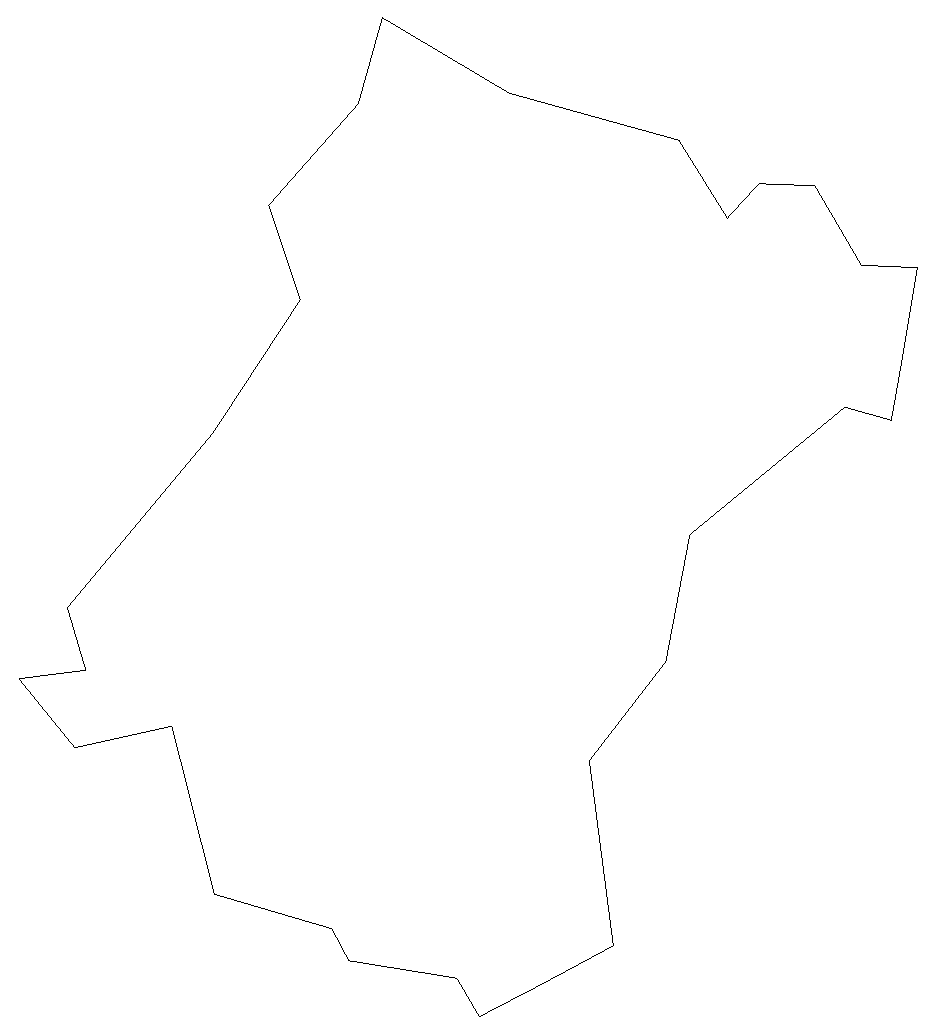
\includegraphics [scale=0.3]{grafiken/westpart.eps}
{\em\caption{\label{partgermany} Corresponding graph of the
section of the boundary file}}
\end{figure}

In some cases it might happen that a region is separated into
subregions that are not connected. As an illustrative example
compare \autoref{westsub} showing a region of Germany that is
separated into 8 subregions. In this case the {\em boundary file}
must contain the polygons of all subregions. The first row for
each of these subregions must contain the region code and the
number of lines the polygon of the respective subregion consists
of. Note that it is not necessary that the polygons of the
subregions are stored in subsequent order in the {\em boundary
file}.

Another special case that might occur is illustrated in
\autoref{westin}. Here a region is completely surrounded by
another region. In this case an additional line must be added to
the boundary description of the {\em surrounded} region. The
additional line must be placed  after the first line and must
contain the
region code of the {\em surrounding} region. The syntax is:

#is.in#,"{\em region code}"

The following lines show a section of the {\em boundary file} of
Germany, where region "9361" is totally
surrounded by region "9371":

\footnotesize

\hspace{1cm} $\vdots$

"9361",7 \\
is.in,"9371" \\
4155.84668,2409.58496 \\
4161.69922,2449.38330 \\
4201.49756,2461.08862 \\
4224.90820,2478.64673 \\
4250.66016,2418.94922 \\
4193.30371,2387.34448 \\
4155.84668,2409.58496

\hspace{1cm} $\vdots$

\normalsize

\begin{figure}[hb]
\centering

\includegraphics [scale=0.3]{grafiken/reg1054.eps}
{\em\caption{\label{westsub} Example for a region that is divided
into subregions}}
\end{figure}

\begin{figure}[hb]
\centering

\includegraphics [scale=0.3]{grafiken/westin.eps}
{\em\caption{\label{westin} Example for a region that is totally
surrounded by another region}}
\end{figure}



Finally, we want to draw attention to an important limitation in
the current version of {\em BayesX}. In most cases {\em map
objects} serve as auxiliary objects to estimate spatial effects
with {\em bayesreg objects} or {\em remlreg objects}. In this case the names of the regions
of the map and the values of the spatial covariate, whose effect
is estimated, must match. Since there are only numerical variables
allowed in {\em dataset objects} (and no string valued variables),
the names of the regions in the corresponding {\em map object}
must necessarily be numbers, although there is in principle no
limitation for the names of regions in {\em map objects}.

\subsubsection*{Structure of a graph file}

A graph file stores the nodes and the edges of a graph $G =
(N,E)$, see for example George and Liu (1981, Ch. 3) for a first
introduction into graph theory. A graph is a convenient way of
representing the neighborhood structure of a geographical map. The
nodes of the graph correspond to the region codes. The
neighborhood structure is represented by the edges of the graph.
In some situations it may be useful to define weights associated
with the edges of a graph which can be stored in the {\em graph
file} as well.

We now describe the structure of a {\em graph file} as it is expected by
{\em BayesX}. The first line of a {\em graph file} must contain
the total number of nodes of the graph. In the remaining lines,
the nodes of the graph together with their edges and associated
weights are specified. One node corresponds to three consecutive
lines. The first of the three lines must contain the name of the
node, which may simply be the name of a geographical region. In
the second line the number of edges of that particular node is
given. The third line contains the corresponding edges of the
node, where an edge is given by the index of a neighboring node.
The index starts with zero. For example, if the fourth and the
seventh node/region in the {\em graph file} are
connected/neighbors, the edge index for the fourth node/region is
6 and for the seventh node/region 3.

We illustrate the structure of a {\em graph file} with an example. The
following few lines are the beginning
of the {\em graph file} corresponding to the map of (former) West Germany:

\footnotesize

327 \\
9162 \\
3 \\
1 2 3 \\
9174 \\
6 \\
0 4 2 3 5 6 \\
9179 \\
6 \\
0 1 7 3 8 6

\hspace{1cm} $\vdots$

\normalsize

\vspace{0.5cm}

The first line specifies the total number of nodes, in the present
example 327 nodes. The subsequent three lines correspond to the
node with name '9162', which is the first region in the map of
West Germany. Region '9162' has 3 neighbors, namely the second,
third and fourth node appearing in the graph file. Once again,
note that the index starts with zero, i.e. 0 corresponds to the
first node, 1 corresponds to the second node and so on. Lines 5 to
7 in the example correspond to node '9174' and its neighbors and
lines 8 to 10 correspond to node '9179'.

In a {\em graph file} it is also possible to specify weights associated
with the edges of the nodes. Since in the preceding example no
weights are explicitly specified, all weights are automatically
defined to be equal to one. Nonequal weights are specified in the
{\em graph file} by simply adding them following the edges of a
particular node.
An example of the beginning of a {\em graph file} with weights is given below:

\footnotesize

327 \\
9162 \\
3 \\
1 2 3 0.4 1.2 0.7\\
9174 \\
6 \\
0 4 2 3 5 6 0.4 0.3 0.8 0.8 1.4 1.6\\
9179 \\
6 \\
0 1 7 3 8 6 1.2 0.8 0.2 1.8 1.7 1.3

\hspace{1cm} $\vdots$

\normalsize

\vspace{0.5cm}

Here the edges of the first node '9162' have weights 0.4, 1.2 and
0.7.\bigskip



\subheader{Options}

\begin{itemize}
\item #graph# \\
If #graph# is specified as an additional option, {\em BayesX}
expects a {\em graph file} to be read in rather than a {\em
boundary file}.
\item #weightdef=adjacency# $|$ #centroid#  $|$ #combnd# \\
\label{weightsmap} Option #weightdef# allows to specify how the
weights associated with each pair of neighbors are computed.
Currently there are three weight specifications available,
#weightdef=adjacency#, #weightdef=centroid# and
#weightdef=combnd#. If #weightdef=adjacency# is specified, for
each pair of neighbors the weights are set equal to one. The so
called adjacency weights are the most common ones in spatial
statistics. Specifying #weightdef=centroid# results in weights
proportional to the distance of the centroids of neighboring
regions. More specifically, the weight $w_{us}$ of two neighboring
regions $u$ and $s$ is set to $w_{us} = c \cdot \exp(-d(u,s))$,
where $d$ is the Euclidian distance between the centroids of the
two sites and $c$ is a normalizing constant. The constant $c$ is
chosen in such a way that the total sum of weights is equal to the
total number of neighbors, which is in analogy to adjacency
weights. The third choice #weightdef=combnd# results in weights
proportional to the length of the common boundary. Similarly to
#weightdef=centroid#, the weights are normalized, i.e. the total
sum of weights is equal to the number of neighbors.

Note that the specification of the #weightdef# option is only
meaningful if a {\em boundary file} is read. If a {\em graph file}
is read  instead, the option has no effect because the boundary
information of regions is missing and  the computation of weights
is therefore impossible.
\end{itemize}



\clearpage



\section{Method outfile}
\label{mapoutfile} \index{map object!outfile command}

\begin{stanza}{Description}

{Method #outfile# performs the reverse of the #infile# command.
Using method #outfile#, the map information currently in memory is
written to an external file. The map information can be written
either in {\em boundary file} or in {\em graph file} format.}
\end{stanza}

\begin{stanza}{Syntax}

{#># {\em objectname}.#outfile# [{\em , options}] #using# {\em
filename}

#outfile# writes the map information to the external file
specified in {\em filename}. The file format can be either a {\em
boundary file} or a {\em graph file}. If #graph# is specified as
an additional option, the file format will be a {\em graph file},
otherwise a {\em boundary file}.}
\end{stanza}

\subheader{Options}

\begin{itemize}
\item #graph# \\
Forces the program to store the map information in {\em graph
file} format rather than {\em boundary file} format.
\item #includeweights# \\
Option #includeweights# is meaningful only if the storing format
is a {\em graph file}, i.e. option #graph# is additionally
specified. In that case the weights associated with the edges
(neighbors) of the nodes (regions) are additionally stored.
\item #replace# \\
The #replace# option allows {\em BayesX} to overwrite an already
existing file. If #replace# is omitted in the optionlist and the
file specified in {\em filename} already exists, an error will be
raised. This prevents you from overwriting an existing file
unintentionally.
\end{itemize}



\clearpage



\section{Method reorder}
\label{mapreorder} \index{reorder regions of a map} \index{map
object!reorder command}

\begin{stanza}{Description}

{Method #reorder# reorders the regions of a map in the sense that
the adjacency matrix of the reordered map has the smallest
envelope when compared to all other possible orderings. A new map
should always be reordered before using it with {\em bayesreg
objects} because MCMC updates for spatial covariates will be much
faster if the envelope of the posterior precision matrix is small.
For reordering of the regions of the map the reverse Cuthill
Mc-Kee algorithm is used, see George and Liu (1981) p. 58 ff.}
\end{stanza}

\begin{stanza}{Syntax}

{#># {\em objectname}.#reorder#

#reorder# reorders the regions of a map in order to obtain
smallest envelope of the corresponding adjacency matrix.}
\end{stanza}

\begin{stanza}{Options}

{Not allowed.}
\end{stanza}

\begin{stanza}{Reference}

{\begin{description}

\item[George, A., Liu, J. W. (1981).] {\em Computer Solution of Large
Sparse Positive Definite Systems.} Series in computational
mathematics, Prentice--Hall.

\end{description}}
\end{stanza}


\chapter{graph objects}
\label{graphobj} \index{Graph object} \index{Visualizing data}

{\em Graph objects} are used to visualize data or estimation results obtained with the regression objects in the GUI
version of {\em BayesX}. No graph objects are available in the command line version of {\it BayesX}. However, the R package
accompanying {\it BayesX} provides similar functionality for visualising data and estimation results as implemented for {\it
graph objects}.

Currently, {\em graph objects} can be used to draw scatterplots between variables (\autoref{graphplot}, method #plot#), or to
draw and color geographical maps stored in {\em map objects} (\autoref{graphdrawmap}, method #drawmap#). The resulting plots
are either printed on the screen or stored as postscript files for further use in other documents (e.g. \LaTeX\/ documents).

A {\em graph object} is created by typing

#> graph# {\em objectname}

in the {\em command window}.


\clearpage


\section{Method drawmap}
\label{graphdrawmap} \index{Graph object!Drawmap command}
\index{Drawing geographical maps}

\begin{stanza}{Description}

Method #drawmap# is used to draw geographical maps and color the
regions according to some numerical characteristics.
\end{stanza}

\begin{stanza}{Syntax}

 #> #{\em objectname}.#drawmap#  [{\em plotvar regionvar}] [#if# {\em expression}], {\em #map#=mapname} [{\em options}]\\
 #> #[#using# {\em dataset}]

Method #drawmap# draws the map stored in the {\em map object} {\em
mapname} and prints the graph either on the screen or stores it as
a postscript file (if option #outfile# is specified). The regions
with regioncode {\em regionvar} are colored according to the
values of the variable {\em plotvar}. The variables {\em plotvar}
and {\em regionvar} are supposed to be stored in the {\em dataset
object} {\em dataset}. An #if# statement may be specified to use
only a part of the data in {\em dataset}. Several options are
available, e.g. for changing from grey scale to color scale or to
store the map as a postscript file. See the options list below for
more details.
\end{stanza}

\begin{stanza}{Options}

The most important option, which therefore is obligatory, is the
#map# option. This option specified the name of the {\em map
object} containing the boundary information to be drawn.
Additional options for method #drawmap# (in alphabetical order)
are:
\end{stanza}

\begin{itemize}
\item #color#

The #color# option allows to choose between a grey scale and a
colored scale. If the keyword #color# is specified, a colored
scale is used instead of a grey scale.

\item #drawnames#

In some situations it may be useful to print the names of the
regions into the graph (although the result will probably be
confusing in most cases). This can be achieved by specifying the
additional option #drawnames#. By default the names of the regions
are omitted in the map.

\item #fontsize = #{\em integer}

Specifies the font size (in pixels) for labelling the legend and
writing the names of the regions (if specified). Note, that the
title is scaled accordingly (see option #titlesize#). The default is
#fontsize=12#.

\item #hcl#

Requests that a color palette from the HCL color space should be
used instead of an RGB palette. The HCL colors will be selected
diverging from a neutral center (grey) to two different extreme
colors (red and green) in contrast to the RGB colors diverging
from yellow to red and green. HCL colors are particularly useful
for electronic presentations since they are device-independent.
The option #hcl# is only meaningful in combination with the option
#color#.

\item #lowerlimit = #{\em realvalue}

Lower limit of the range to be drawn. If #lowerlimit# is omitted,
the minimum numerical value in {\em plotvar} will be used as the
lower limit instead.

\item #map = #{\em mapname}

{\em mapname} specifies the name of the {\em map object}
containing the boundary information to be drawn. This option is
obligatory.

\item #nolegend#

By default a legend is drawn into the graph. Specifying the option
#nolegend# will exclude the legend from the graph.

\item #nrcolors = #{\em integer}

To color the regions according to their numerical characteristics,
the data are divided into a (typically large) number of ordered
categories. Afterwards a color is associated with each category.
The #nrcolors# option can be used to specify the number of
categories (and therefore the number of different colors). The
maximum number of colors is 256, which is also the default value.

\item #outfile = #{\em filename}

If option #outfile# is specified the graph will be stored as a
postscript file rather than being printed on the screen. The full
path and the filename have to be specified in {\em filename}. By
default, an error will be raised if the specified file is already
existing or if the path is invalid. To overwrite  an already
existing file, option #replace# has to be specified in addition.
This prevents you from overwriting your files unintentionally.

\item #pcat#

If you want to visualize posterior probabilities, it is convenient
to specify #pcat#. In this case, method #drawmap# expects a
variable containing only the values -1, 0 and 1. Of course you can
achieve the same result by setting #nrcolors=3#, #lowerlimit=-1#
and #upperlimit=1#.

\item #replace#

The #replace# option is only meanigful in combination with option
#outfile#. Specifying #replace# as an additional option allows the
program to overwrite an already existing file (specified in
#outfile#), otherwise an error will be raised.

\item #swapcolors#

In some situations it may be favorable to swap the order of the
colors, i.e. black (red) shades corresponding to large values and
white (green) shades corresponding to small values. This is
achieved by specifying #swapcolors#. By default, small values are
colored in black shades (red shades) and large values in white
shades (green shades).

\item #title = #{\em characterstring}

Adds a title to the graph. If the title contains more than one
word, {\em characterstring} must be enclosed by quotation marks
(e.g. #title="my first map"#).

\item #titlesize = #{\em realvalue}

Specifies the factor by which the size of the title is scaled
relative to the size of the labels of the legend (compare option
#fontsize#). The default is #titlesize=1.5#.

\item #upperlimit = #{\em realvalue}

Upper limit of the range to be drawn. If #upperlimit# is omitted,
the maximum numerical value in {\em plotvar} will be used as the
upper limit instead.

\end{itemize}

\begin{stanza}{Example}

This example shows how to draw the map of Munich and how to color
the subquarters in Munich according to some numerical
characteristics. The boundary file of Munich (#munich.bnd#) as
well as the data set #rent94means.raw# containing the distribution
of the average rents across subquarters are included in the
subfolder #examples# of the {\em BayesX} installation directory.
In the following we assume that {\em BayesX} is installed in the
folder #c:\bayesx#. We start by creating a {\em dataset object}
#d# and a {\em map object} #m# and proceed with reading the rent
data set and the map of Munich:

#> dataset d# \\
#> d.infile using c:\bayesx\examples\rent94means.raw#

#> map m# \\
#> m.infile using c:\bayesx\examples\munich.bnd#

Afterwards we create a {\em graph object} #g# and draw the map of
Munich:

#> graph g# \\
#> g.drawmap , map=m#

\begin{figure}[htb]
\begin{center}
\includegraphics[scale=0.5]{grafiken/munichdrawmap.ps}
{\em\caption{ \label{munichdrawmap} Map of Munich}}
\end{center}
\end{figure}

The map of Munich appears on the screen in a separate window,
compare \autoref{munichdrawmap}. Before closing the window you are
asked whether you want to save the map or not. If you agree the
map will be stored as a postscript file in the folder you specify.
Of course, the map can be directly stored in postscript format
using the #outfile# option. In this case the map is not shown on
the screen. Typing

#> g.drawmap , map=m outfile=c:\temp\munich.ps#

stores the map of Munich in the file #c:\temp\munich.ps# and the
graph is not printed on the screen.

Usually maps are drawn to visualize numerical characteristics of
their regions. For instance, typing

#> g.drawmap R L , map=m color using d#

displays the distribution of the average rents #R# across
subquarters #L#, see \autoref{munichmeans}. The areas in the
figure shaded with diagonal lines mark subquarters for which  no
data are available. The specification of the second variable #L#
is required to match the names of the subquarters stored in the
{\em map object} #m# with the data set #d#. Option #color# is
specified to obtain a colored graph. Specifying option #hcl# in
addition yields the same information visualized in HCL colors (see
\autoref{munichmeanshcl}).

#> g.drawmap R L , map=m color hcl using d#

\end{stanza}

\begin{figure}[htb]
\begin{center}
\includegraphics[scale=0.5]{grafiken/munichmeansdrawmap.ps}
{\em\caption{ \label{munichmeans} Distribution of the average rents
per square meter in Munich visualized in RGB colors.}}
\end{center}
\end{figure}

\begin{figure}[htb]
\begin{center}
\includegraphics[scale=0.5]{grafiken/munichmeansdrawmaphcl.ps}
{\em\caption{ \label{munichmeanshcl} Distribution of the average
rents per square meter in Munich visualized in HCL colors.}}
\end{center}
\end{figure}

\clearpage

\section{Method plot}
\label{graphplot} \index{Graph object!Plot command}
\index{Scatterplot} \index{Drawing scatterplots}

\begin{stanza}{Description}

{Method #plot# is used to draw scatterplots between two or more
variables. Several options for labelling axes, connecting points,
saving the graph etc. are available.}
\end{stanza}

\begin{stanza}{Syntax}

{#> #{\em objectname}.#plot#  {\em xvar yvar1} [{\em yvar2 yvar3}
\dots]
[#if# {\em expression}] [, {\em options}] #using# {\em dataset}

Method #plot# draws scatterplots of {\em yvar1}, {\em yvar2}, {\em
yvar3} $\dots$ against {\em xvar} into a single graph using the
data set specified in {\em dataset}. An #if# statement may be used
to apply the method only to a part of the data. In addition,
several options may be specified for labelling axes, connecting
points, saving the graph in postscript format etc., see the
options list below.}
\end{stanza}

\begin{stanza}{Options}

{The following options are available for method #plot# (listed in
alphabetical order):}
\end{stanza}

\begin{itemize}
\item #connect = 1#$|$#2#$|$#3#$|$#4#$|$#5#[{\em specifications
for further variables}]

Option #connect# specifies how points in the scatterplot are
connected. There are currently 5 different specifications:

\begin{tabular}{ll}
#1# & draw straight lines between the points (default) \\
#2#, #3#, #4# & draw dashed lines (numbers 2 -- 4 indicate different variants)\\
#5# & do not connect, i.e.~plot points only \\
\end{tabular}

If you draw more than one scatterplot in the same graph (i.e. more
than one {\em yvar} is specified) the points for each {\em yvar}
can be connected differently by specifying the corresponding
number (#1,2,3,4,5#) separately for every {\em yvar}. Typing for
example

#connect=15#

connects the points corresponding to {\em yvar1} and {\em xvar} by
straight lines, but does not connect the points corresponding to
{\em yvar2} (if specified) and {\em xvar}. Points corresponding to
additional variables $yvar3$, etc.~are connected by straight lines
(the default).

An equivalent way of specifying the different variants is
available via the symbols '#l#', '#d#', '#_#', '#-#' and '#p#',
which correspond to the numbers 1-5, i.e.~

#connect=12345# is equivalent to #connect=ld_-p#

\item #fontsize = #{\em integer}

Specifies the font size (in pixels) for labelling axes etc. Note
that the title is scaled accordingly. The default is
#fontsize=12#.

\item #height = #{\em integer}

Specifies the height (in pixels) of the graph. The default is
#height=210#.

 \item #linecolor = B#$|$#b#$|$#c#$|$#G#$|$#g#$|$#o#$|$#m#$|$#r#$|$#y# [{\em specifications
for further variables}]

Option #linecolor# specifies the color to be used for drawing
lines (or points, see option #connect#) in the scatterplot.
Currently the following specifications are available:

\begin{tabular}{ll}
#B# & black (default) \\
#b# & blue \\
#c# & cyan \\
#G# & gray \\
#g# & green \\
#o# & orange \\
#m# & magenta \\
#r# & red \\
#y# & yellow \\
\end{tabular}

If you draw more than one scatterplot in the same graph (i.e. more
than one {\em yvar} is specified) you can use different colors for
each {\em yvar} by simply specifying the corresponding symbol
(#B,b,c,G,g,o,m,r,y#) for each {\em yvar}. Typing for example

#linecolor = Bgr#

colors the lines (points) corresponding to {\em yvar1} and {\em
xvar} in black, whereas the points corresponding to {\em yvar2}
and {\em yvar3} (if specified) and {\em xvar} are colored in green
and red, respectively.

\item #linewidth = #{\em integer}

Specifies how thick lines should be drawn. The default is
#linewidth=5#.

\item #outfile = #{\em filename}

If option #outfile# is specified, the graph will be stored as a
postscript file rather than being printed on the screen. The full
path and the filename have to be specified in {\em filename}. By
default, an error will be raised if the specified file is already
existing or if the specified folder is not valid. To overwrite an
already existing file, option #replace# must be specified in
addition. This prevents you from overwriting your files
unintentionally.

\item #pointsize = #{\em integer}

Specifies the size of the points (in pixels) if drawing points
rather than lines. The default is #pointsize=20#.

\item #replace#

The #replace# option is useful only in combination with option
#outfile#. Specifying #replace# as an additional option allows the
program to overwrite an already existing file (specified in
#outfile#), otherwise an error will be raised.

\item #title = #{\em characterstring}

Adds a title to the graph. If the title contains more than one
word, {\em characterstring} must be enclosed by quotation marks (e.g.
#title="my first title"#).

\item #titlesize = #{\em realvalue}

Specifies the factor by which the size of the title is scaled
relative to the size of the labels of the axes (compare option
#fontsize#). The default is #titlesize=1.5#.

\item #width = #{\em integer}

Specifies the width (in pixels) of the graph. The default is
#width=356#.

\item #xlab = #{\em characterstring}

Labels the x-axis. If the label contains more than one word, {\em
characterstring} must be enclosed by quotation marks (e.g.
#xlab="x axis"#).

\item #xlimbottom = #{\em realvalue}

Specifies the minimum value at the x-axis to be drawn. The default
is the minimum value in the data set. If #xlimbottom# is above the
minimum value in the data set, only a part of the  graph will be
visible.

\item #xlimtop = #{\em realvalue}

Specifies the maximum value at the x-axis to be drawn. The default
is the maximum value in the data set. If #xlimtop# is below the
maximum value in the data set, only a part of the  graph will be
visible.

\item #xstart = #{\em realvalue}

Specifies the value where the first tick on the x-axis should be
drawn. The default is the minimum value on the x-axis.

\item #xstep = #{\em realvalue}

If #xstep# is specified, ticks are drawn at the x-axis with
stepwidth {\em realvalue} starting at the minimum value on the
x-axis (or at the value specified in option #xstart#). By default,
five equally spaced ticks are drawn at the x-axis.

\item #ylab = #{\em characterstring}

Labels the y-axis. If the label contains more than one word, {\em
characterstring} must be enclosed by quotation marks (e.g.
\texttt{ylab="y axis"}).

\item #ylimbottom = #{\em realvalue}

Specifies the minimum value at the y-axis to be drawn. The default
is the minimum value in the data set. If #ylimbottom# is above the
minimum value in the data set, only a part of the  graph will be
visible.

\item #ylimtop = #{\em realvalue}

Specifies the maximum value at the y-axis to be drawn. The default
is the maximum value in the data set. If #ylimtop# is below the
maximum value in the data set, only a part of the  graph will be
visible.

\item #ystart = #{\em realvalue}

Specifies the value where the first tick on the y-axis should be
drawn. The default is the minimum value on the y-axis.

\item #ystep = #{\em realvalue}

If #ystep# is specified,  ticks are drawn at the y-axis with
stepwidth {\em realvalue} starting at the minimum value on the
y-axis (or at the value specified in option #ystart#). By default,
five equally spaced ticks are drawn at the y-axis.

\item Further options for representing dates

In the following we describe options that may be useful if the
variable on the x-axis represents dates. An example is a variable
with values ranging from 1 to 19, representing the time period
from January 1983 to July 1984. In this case, we might prefer that
the x-axis is labelled in terms of dates rather than in the
original coding (from 1 to 19). To achieve this, {\em BayesX}
provides the options #month#, #year# and #xstep#. Options #year#
and #month# are used to specify the year and the month (1 for
January, 2 for February, \dots) corresponding to the minimum
covariate value. In the example mentioned above #year=1983# and
#month=1# will produce the correct result. In addition, option
#xstep# may be specified to define the periodicity in which your
data are collected. For example #xstep=12# (the default)
corresponds to monthly data, while #xstep = 4#, #xstep = 2# and
#xstep = 1# correspond to quarterly, half yearly and yearly data,
respectively.
\end{itemize}


\begin{stanza}{Example}

{We use the Munich rent data set #rent94.raw# to demonstrate the
usage of method #plot#. The data set is included in the subfolder
#examples# of the {\em BayesX} installation directory. In the
following we assume that {\em BayesX} has been installed to the
folder #c:\bayesx#. We start by reading the data by typing:

#> dataset d# \\
#> d.infile using c:\bayesx\examples\rent94.raw#

Then we generate a {\em graph object} #g# and draw a scatterplot
between floor space (variable #F#) and rent per square meter
(variable #R#):

#> graph g# \\
#> g.plot R F using d#

The strange picture shown in \autoref{plotrf1} appears on the
screen. The problem is that the points are connected by straight
lines although the values of #F# are not sorted. Hence, to obtain
an improved scatterplot, we could either sort the data set with
respect to #F# or simply avoid connecting the points. Typing

#> d.sort F# \\
#> g.plot R F using d#

yields the first option. Typing

#> g.plot R F, connect=p using d#

yields the second option mentioned above. The corresponding graphs
are shown in \autoref{plotrf2} and \autoref{plotrf3},
respectively. To further improve the appearance of the scatterplot
we add a title and label the x- and y-axes
by typing

#> g.plot R F, title="scatterplot between F and R" ylab="rent"# \\
#  xlab="floor space in square meters" connect=p using d#

The result is shown in \autoref{plotrf4}.
Finally, we add the outfile option to save the graph in postscript format:

 #> g.plot R F, title="scatterplot between F and R" ylab="rent" #\\
 #  xlab="floor space in square meters" connect=p#\\
 #  outfile=c:\temp\plotrf.ps using d #

\begin{figure}[ht]
\begin{center}
\includegraphics[scale=0.7]{grafiken/plotrf1.ps}
{\em\caption{ \label{plotrf1} Scatterplot between floor space and
rent per square meters (first try).}}
\end{center}
\end{figure}

\begin{figure}[ht]
\begin{center}
\includegraphics[scale=0.7]{grafiken/plotrf2.ps}
{\em\caption{ \label{plotrf2} Scatterplot between floor space and
rent per square meters (second try).}}
\end{center}
\end{figure}

\begin{figure}[ht]
\begin{center}
\includegraphics[scale=0.7]{grafiken/plotrf3.ps}
{\em\caption{ \label{plotrf3} Scatterplot between floor space and
rent per square meters (third try).}}
\end{center}
\end{figure}

\begin{figure}[ht]
\begin{center}
\includegraphics[scale=0.7]{grafiken/plotrf4.ps}
{\em\caption{ \label{plotrf4} Scatterplot between floor space and
rent per square meters (final try).}}
\end{center}
\end{figure}
}
\end{stanza}
\clearpage



\clearpage



\section{Method plotautocor}
\label{graphplotautocor} \index{Graph object!Plotautocor command}
\index{Plotting autocorrelations}

\begin{stanza}{Description}

{Method #plotautocor# visualizes the autocorrelation functions
obtained with method #autocor# of {\em bayesreg objects}, see also
\autoref{bayesautocorr}.}
\end{stanza}


\begin{stanza}{Syntax}

{#> #{\em objectname}.#plotautocor# [,{\em options}] #using# {\em dataset}

Plots the autocorrelation functions stored in {\em dataset}. The
data set must have the special structure described in
\autoref{bayesautocorr}, i.e. method #plotautocor# is meaningful
only if Bayesian regression models have been estimated in advance
using {\em bayesreg objects} and autocorrelation functions of
sampled parameters have been computed using method #autocor# of
{\em bayesreg objects}.}
\end{stanza}

\subheader{Options}

\begin{itemize}
\item #mean#

If option #mean# is specified, only minimum, mean and maximum
autocorrelations are plotted for each lag number and model term.
This typically leads to a considerable reduction in computing time
and storing size.

\item #outfile = #{\em filename}

If option #outfile# is specified, the graph will be stored as a
postscript file instead of being printed on the screen. The path
and the filename have to be specified in {\em filename}. An error
will be raised if the specified file is already existing and the
#replace# option has not been specified.

\item #replace#

The #replace# option is only meaningful in combination with option
#outfile#. Specifying #replace# as an additional option allows the
program to overwrite an already existing file (specified in
#outfile#), otherwise an error will be raised.
\end{itemize}



\clearpage



\section{Method plotsample}
\label{graphplotsample} \index{Graph object!Plotsample command}
\index{Plotting sampled parameters} \index{Sampling paths}

\begin{stanza}{Description}

{Method #plotsample# visualizes the sampling paths of sampled
parameters obtained with method #getsample# of {\em bayesreg
objects}, see also \autoref{bayesgetsample}. The application of
method #plotsample# is meaningful only if Bayesian regression
models have been estimated in advance using {\em bayesreg objects}
and sampled parameters have been computed and stored using method
#getsample#.}
\end{stanza}

\begin{stanza}{Syntax}

{#> #{\em objectname}.#plotsample# [,{\em options}] #using# {\em dataset}

Plots sampled parameters stored in {\em dataset}. The data set
must have the special structure described in
\autoref{bayesgetsample}.}
\end{stanza}

\subheader{Options}

\begin{itemize}
\item #outfile = #{\em filename}

If option #outfile# is specified, the graph will be stored as a
postscript file instead of being printed on the screen. The full
path and the filename have to be specified in {\em filename}. An
error will be raised if the specified file is already existing and
the #replace# option has not been specified.

\item #replace#

The #replace# option is only useful in combination with option
#outfile#. Specifying #replace# as an additional option allows the
program to overwrite an already existing file (specified in
#outfile#), otherwise an error will be raised.
\end{itemize}


\chapter{bayesreg objects}
\label{bayesreg} \index{Bayesreg object}

{\em bayesreg objects} are used to fit (multivariate) exponential family, hazard rate or multi-state models with {\em
structured additive predictor} subsumed in the class of {\em structured additive regression (STAR)} models, see \citeasnoun{FahKneLan04}.
Inference is based on fully Bayesian approach implemented via Markov Chain Monte Carlo (MCMC)
simulation techniques. The methodology manual provides brief introduction to structured additive regression and MCMC-based
inference. More details can be found in \citeasnoun{FahLan01a}, \citeasnoun{FahLan01b}, \citeasnoun{LanBre04},
\citeasnoun{BreLan06}, \citeasnoun{FahOsu03} and \citeasnoun{HenBreFah06}. Good introductions to
generalized linear models are the monographs of \citeasnoun{FahTut01} and \citeasnoun{McCNel89}. Introductions to semi- and
nonparametric models are given in \citeasnoun{GreSil94}, \citeasnoun{HasTib90}, \citeasnoun{HasTibFri01} or \citeasnoun{Woo06a}.
The paper of \citeasnoun{ChiGre95}, the monograph {\em Markov Chain Monte Carlo in Practice} edited by
\citeasnoun{GilRicSpi96} and the introductory article by \citeasnoun{Gre01} give a thorough overview over MCMC simulation
techniques.

First steps with {\em bayesreg objects} can be done with the
tutorial like example in chapter \ref*{zambiaanalysis} of the
tutorials manual which provides a self-contained demonstrating
example.

\clearpage

\section{Method regress}
\label{bayesregress} \index{Bayesreg object!Regress
function}\index{Regress function}

\subsection{Description}
\label{bayesregregressdescr}

Method #regress# estimates a structured additive regression model.

\index{Generalized linear models} \index{Generalized additive
models} \index{Varying coefficients} \index{Bayesian semiparametric
regression} \index{MCMC} \index{Markov chain Monte Carlo}

\subsection{Syntax}\index{Regression syntax}\index{Bayesreg object!Regression syntax}
\label{bayesregregresssyntax}

 #> #{\em objectname}.#regress# {\em model} [#weight# {\em weightvar}] [#if# {\em expression}] [{\em , options}] #using# {\em dataset}

Method #regress# estimates the regression model specified in {\em
model} using the data specified in {\em dataset}. {\em dataset}
has to be the name of a {\em dataset object} created before. The
details of correct models are covered in \autoref{modelsyntax}.
The distribution of the response variable can be either Gaussian,
gamma, binomial, multinomial, Poisson, negative binomial, zero
inflated Poisson or zero inflated negative binomial. In addition,
{\em BayesX} supports continuous time survival and multi-state
models, see also \autoref{familyopt} for a more detailled
overview. The response distribution is specified using option
#family#, see \autoref{familysyntax} below and the options list in
\autoref{regressoptions}. The default value is #family=binomial#
with a logit link. An #if# statement may be specified to analyze
only parts of the data set, i.e.~the observations where {\em
expression} is true.

\subsubsection{Optional weight variable}\index{Weighted regression}
\label{weightspecification}

An optional weight variable {\em weightvar} may be specified to
estimate weighted regression models. For Gaussian responses {\em
BayesX} assumes that $y_r|\eta_r,\sigma^2 \sim
N(\eta,\sigma^2/weightvar_r)$. Thus, for grouped Gaussian
responses the weights must be the number of observations in the
groups if the $y_r$'s are the average of individual responses. If
the $y_r$'s are the sum of responses in every group, the weights
have to be the reciprocal of the number of observations in the
groups. Of course, estimation of usual weighted regression models
with heteroscedastic errors is also possible. In this case the
weights should be proportional to the reciprocal of the
heteroscedastic variances. If the response distribution is
binomial, it is assumed that the values of the weight variable
correspond to the number of replications and that the values of
the response variable itself correspond to the number of
successes. If #weight# is omitted, {\em BayesX} assumes that the
number of replications is one, i.e.~the values of the response
must be either zero or one. For grouped Poisson data the weights
have to be the number of observations in a group and the $y_i$'s
are assumed to be the average of individual responses. In the case
of gamma distributed responses, {\em BayesX} assumes $y_r \sim
G(\exp(\eta_r),\nu/weightvar_r)$ where $\mu_r= \exp(\eta_r)$ is
the mean and $s_r = \nu/weightvar_r$ is the scale parameter.

If estimation is based on latent utility representations, the
specification of weights is not allowed. Similarly, for negative
binomial, zero inflated Poisson and zero inflated negative
binomial models as well as hazard regression and multi-state
models, weighted regression is not implemented yet.

\subsubsection{Syntax of possible model terms}
\label{modelsyntax}\index{Model terms}\index{Bayesreg object!Model
terms}

The general syntax of models is:

$depvar = term_1 + term_2 + \cdots + term_r$

where {\em depvar} specifies the dependent variable in the model
and $term_1$,\dots,$term_r$ define the specific form of covariate
effects on the dependent variable. The different terms have to be
separated by '+' signs. A constant intercept is automatically
included in the models and does not have to be requested by the
user. This section reviews all possible model terms that are
currently supported by {\em bayesreg objects} and provides some
specific examples. Note that all described terms may be combined
in arbitrary order. An overview about the capabilities of {\em
bayesreg objects} is given in \autoref{terms}.
\autoref{bayesreginteractions} shows how interactions between
covariates are specified. Full details about all available options
are given in \autoref{localoptions}.

Throughout this section #Y# will denote the dependent variable.

\subsubsection*{Offset}\index{Offset}

\begin{itemize}
\item[] {\em Description}: Adds an offset term to the predictor.
\item[] {\em Predictor}: $\eta =  \cdots + \mbox{\it offs} + \cdots$
\item[] {\em Syntax}: #offs(offset)#
\item[] {\em Example}:

The following model statement can be used to estimate a Poisson
model with #offs# as offset term and #W1# and #W2# as fixed
effects (if #family=poisson# is specified in addition):

#Y = offs(offset) + W1 + W2#

\end{itemize}

\subsubsection*{Fixed effects}\index{Fixed effects}

\begin{itemize}
\item[] {\em Description}: Incorporates covariate #W1# as a fixed effect into the model.
\item[] {\em Predictor}: $\eta =  \cdots + \gamma_1 W1 + \cdots$
\item[] {\em Syntax}: #W1#
\item[] {\em Example}:

The following model statement specified a model with $q$ fixed
(linear) effects:

\texttt{Y = W1 + W2 + $\cdots$ + Wq}
\end{itemize}

\subsubsection*{Nonlinear effects of continuous covariates and time
scales}\index{Nonlinear effects}\index{Random
walks}\index{P-splines}


\begin{itemize}
 \item[]{\bf\sffamily First or second order random walk}
 \item[]{\em Description}: Defines a first or second order random walk
 prior for the effect of #X1#.
 \item[]{\em Predictor}: $\eta = \cdots + f_1(X1) + \cdots $
 \item[] {\em Syntax}:

#X1(rw1#[, {\em options}]#) #

#X1(rw2#[, {\em options}]#) #
\item[] {\em Example}:

Suppose that #X1# is a continuous covariate with possibly
nonlinear effect. The following model statement defines a second
order random walk prior for $f_1$:

#Y = X1(rw2,a=0.001,b=0.001)#

The term #X1(rw2,a=0.001,b=0.001)# indicates, that the effect of
#X1# should be included nonparametrically using a second order
random walk prior. A first order random walk is obtained by
modifying the first argument in #X1(rw2,a=0.001,b=0.001)# from
#rw2# to #rw1# yielding #X1(rw1,a=0.001,b=0.001)#. The second and
third argument in the expression above are used to specify the
hyperparameters of the inverse gamma prior for the variance of the
random walk. Besides the options #a# and #b#, some more options
are available, see \autoref{localoptions} for details.

\item[] {\bf\sffamily P-spline with first or second order random
walk penalty}

\item[] {\em Description}: Defines a P-spline with a first or
second order random walk penalty for the parameters of the spline.
\item[] {\em Predictor}: $\eta =  \cdots + f_1(X1) + \cdots$
\item[] {\em Syntax}:

#X1(psplinerw1#[{\em , options}]#) #

#X1(psplinerw2#[{\em , options}]#) #
\item[] {\em Example}:

A P-spline with second order random walk penalty is obtained by:

#Y = X1(psplinerw2)#

By default, the degree of the spline is 3 and the number of inner
knots is 20. The following model term defines a quadratic P-spline
with 30 knots:

#Y = X1(psplinerw2,degree=2,nrknots=30)#

Full details about all possible options for P-splines are given in
\autoref{localoptions}.

\item[] {\bf\sffamily Seasonal effect of a time scale}

\item[] {\em Description}: Defines a seasonal effect of #time#.
\item[] {\em Predictor}: $\eta =  \cdots + f_{season}(time) +
\cdots $ \item[] {\em Syntax}:

#time(season#[, {\em options}]#) #
\item[] {\em Example}:

A seasonal component for a time scale #time# is specified by

#Y = time(season,period=12)#.

where the second argument specifies the period of the seasonal
effect. In the example above the period is 12, corresponding to
monthly data.
\end{itemize}


\subsubsection*{Spatial Covariates}\index{Spatial
effects}\index{Markov random fields}\index{Two-dimensional P-spline}

\begin{itemize}
\item[]{\bf\sffamily Markov random field}

\item[] {\em Description}:

Defines a Markov random field prior for the spatial covariate
#region#. {\em BayesX} allows to incorporate spatial covariates
with geographical information stored in the {\em map object}
specified in option #map#.

\item[] {\em Predictor}: $\eta = \cdots + f_{spat}(region) +
\cdots$

\item[] {\em Syntax}:

#region(spatial,map=#{\em characterstring}#[#{\em , options}]#) #
\item[] {\em Example}:

For the specification of a Markov random field prior, #map# is an
obligatory argument that represents the name of a {\em map object}
(see \autoref{map}) containing all necessary spatial information
about the geographical map, i.e.~the neighbors of each region and
the weights associated with the neighbors. For example the
statement

#Y = region(spatial,map=germany)#

defines a Markov random field prior for #region# where the
geographical information is stored in the {\em map object}
#germany#. An error will be raised if #germany# is not existing.
It is advisable to reorder the regions of a map prior to
estimation of a spatial effect to obtain a band matrix like
precision matrix. This can be achieved using method #reorder# of
{\em map objects}, see \autoref{mapreorder} for details.

\item[]{\bf\sffamily Two-dimensional P-spline with first order
random walk penalty}

\item[] {\em Description}:

Defines a two-dimensional P-spline for the spatial covariate
#region# with a two-dimensional first order random walk penalty
for the parameters of the spline. Estimation is based on the
coordinates of the centroids of the regions. The centroids are
computed using the geographical information stored in the {\em map
object} specified in the option #map#.

\item[] {\em Predictor}: $\eta= \cdots + f(centroids) + \cdots$

\item[] {\em Syntax}:

#region(geospline,map=#{\em characterstring}#[, #{\em options}]#) #
\item[] {\em Example}:

For the specification of a two-dimensional P-spline ({\em
geospline}) #map# is an obligatory argument indicating the name of
a {\em map object} (see \autoref{map}) that contains all necessary
spatial information about the geographical map, i.e.~the neighbors
of each region and the weights associated with the neighbors. The
model term

#Y = region(geospline,map=germany)#

specifies a two-dimensional cubic P-spline with first order random
walk penalty where the geographical information is stored in the
{\em map object} #germany#.
\end{itemize}

\subsubsection*{Unordered group indicators}\index{Unordered group
indicators}\index{Random effects}\index{Random intercept}

\begin{itemize}
\item[]{\bf\sffamily Unit- or cluster-specific unstructured
effect}

\item[] {\em Description}: Defines an unstructured (uncorrelated)
random effect with respect to grouping variable #grvar#. \item[]
{\em Predictor}: $\eta = \cdots + f(grvar) + \cdots$ \item[] {\em
Syntax}:

#grvar(random#[, {\em options}]#) #
\item[] {\em Example}:

Gaussian i.i.d.~random effects allow to cope with unobserved
heterogeneity among units or clusters of observations. Suppose the
analyzed data set contains a group indicator #grvar# that gives
information about the individual or cluster a particular
observation belongs to. Then an individual-specific uncorrelated
random effect is defined by

#Y = grvar(random)#

The inclusion of more than one random effect term in the model is
possible, leading to the estimation of multilevel models. However,
we have only limited experience with multilevel models so that it
is not clear how well these models can be estimated in {\em
BayesX}.
\end{itemize}

\subsubsection*{Nonlinear baseline effect in hazard regression or multi-state models}
\index{Baseline}\index{Cox model}\index{Multi-state model}

\begin{itemize}
\item[]{\bf\sffamily P-spline with second order random walk
penalty}

\item[] {\em Description}: Defines a P-spline with second order
random walk penalty for the parameters of the spline for the
log-baseline effect $\log(\lambda_0$(#time#)). \item[] {\em
Predictor}: $\eta = \log(\lambda_0(time)) + \cdots$ \item[] {\em
Syntax}:

#time(baseline#[, {\em options}]#) #
\item[] {\em Example}:

Suppose continuous-time survival data (#time#, #delta#) together
with additional covariates (#W1#,#X1#) are given where #time#
denotes the vector of observed duration times, #delta# is the
vector of corresponding indicators of non-censoring, #W1# is a
discrete covariate, and #X1# is a continuous covariate. The
following continuous time survival model with hazard rate
$\lambda$ and log-baseline effect $\log(\lambda_0$(#time#))
\[
\lambda(time)=\lambda_0(time)\exp (\gamma_0 + \gamma_1 W1 + f(X1)
)=\exp\left(\log(\lambda_0(time)) + \gamma_0 + \gamma_1 W1 +
f(X1)\right)
\]
is estimated by the model statement

#delta = time(baseline) + W1 + X1(psplinerw2)#

Similarly, baseline effects on the transition intensities can be
specified in multi-state models.
\end{itemize}

\subsubsection*{Varying coefficients with continuous covariates as
effect modifier}\index{Varying coefficients}

\begin{itemize}
\item[]{\bf\sffamily First or second order random walk}

\item[] {\em Description}:

Defines a varying coefficient term, where the effect of #X1#
varies smoothly over the range of #X2#. Therefore covariate #X2#
is called the effect modifier. The smoothness prior for $f(X2)$ is
a first or second order random walk. \item[] {\em Predictor}:
$\eta= \cdots + f(X2)X1 + \cdots$ \item[] {\em Syntax}:

#X1*X2(rw1#[, {\em options}]#) #

#X1*X2(rw2#[, {\em options}]#) #
\item[] {\em Example}:

A varying coefficient term with a second order random walk
smoothness prior is defined as follows:

#Y = X1*X2(rw2)#

\item[] {\bf\sffamily P-spline with first or second order random
walk penalty}

\item[] {\em Description}:

Defines a varying coefficient term, where the effect of #X1#
varies smoothly over the range of #X2#. The smoothness prior for
$f(X2)$ is a P-spline with first or second order random walk
penalty. \item[] {\em Predictor}: $\eta= \cdots + f(X2)X1 +
\cdots$ \item[] {\em Syntax}:

#X1*X2(psplinerw1#[, {\em options}]#) #

#X1*X2(psplinerw2#[, {\em options}]#) #
\item[] {\em Example}:

A varying coefficient term with a second order random walk
smoothness prior is defined as follows:

#Y = X1*X2(psplinerw2)#

\item[]{\bf\sffamily Seasonal prior}

\item[] {\em Description}:

Defines a varying coefficients term where the effect of #X1#
varies over the range of the effect modifier #time#. A seasonal
prior is assumed for the effect of #time#.

\item[] {\em Predictor}: $\eta= \cdots + f_{season}(time)X1 +
\cdots $

\item[] {\em Syntax}:

#X1*time(season#[, {\em options}]#) #
\item[] {\em Example}:

The inclusion of a varying coefficients term with a seasonal prior
may be meaningful if we expect a different seasonal effect with
respect to a binary variable #X1#. In this case we can include an
additional seasonal effects for observations with #X1#=1 by

#Y = X1*time(season) #

\end{itemize}

\subsubsection*{Time-varying effects in hazard regression or multi-state models}
\index{Time-varying effects}

\begin{itemize}
\item[]{\bf\sffamily P-spline with second order random walk
penalty}

\item[] {\em Description}: Defines a varying coefficients term
where the effect of #X1# varies over the range of the effect
modifier #time#, i.e. variable #X1# is assumed to have a
time-varying effect. The smoothness prior for $f($#time#$)$ is a
P-spline with second order random walk penalty.

 \item[] {\em Predictor}: $\eta = \log(\lambda_0(time)) +
f(time)X1 \cdots$ \item[] {\em Syntax}:

 #X1*time(baseline#[, {\em options}]#) #
 \item[] {\em Example}:

Suppose continuous-time survival data (#time#, #delta#) together
with an additional covariate #X1# are given, where #time# denotes
the vector of observed duration times and #delta# is the vector of
corresponding indicators of non-censoring. The following Cox model
with hazard rate
\begin{eqnarray*}
 \lambda(time) & = & \lambda_0(time)\exp(\gamma_0 + f(time)X1)\\
 & = & \exp\left(\log(\lambda_0(time)) + \gamma_0 + f(time)X1\right)
\end{eqnarray*}
is estimated by the model statement

#delta = time(baseline) + X1*time(baseline)#

Similarly, time-varying effects on the transition intensities can
be specified in multi-state models.
\end{itemize}


\subsubsection*{Varying coefficients with spatial covariates as
effect modifiers}

\begin{itemize}
\item[]{\bf\sffamily Markov random field}

\item[] {\em Description}:

Defines a varying coefficients term where the effect of #X1#
varies smoothly over the range of the spatial covariate #region#.
A Markov random field is estimated for $f_{spat}($#region#$)$. The
geographical information is assumed to be stored in the {\em map
object} specified in the option #map#.

\item[] {\em Predictor}: $\eta = \cdots + f_{spat}(region)X1 +
\cdots$

\item[] {\em Syntax}:

#X1*region(spatial,map=#{\em characterstring}#[,#{\em options}]#) #
\item[] {\em Example}:

The statement

#Y = X1*region(spatial,map=germany) #

defines a varying coefficient term with the spatial covariate
#region# as the effect modifier and a Markov random field as spatial
smoothness prior. Weighted Markov random fields can be estimated by
including an appropriate weight definition when creating the {\em
map object} #germany# (see \autoref{mapinfile}).
\end{itemize}


%{\em Two-dimensional P-spline with first order random walk penalty}
%\begin{itemize}
%\item[] {\em Description}:

%Defines a varying coefficients term where the effect of X1 varies
%smoothly over the range of the spatial covariate X2. A 2
%dimensional P-spline based on the tensor product of one-dimensional
%P-splines with a two-dimensional first order random walk penalty for
%the parameters of the spline is estimated for $f$. The centroids
%are computed using the geographical information stored in the map
%object specified through the option #map#.
%\item[] {\em Predictor}: $\eta= \cdots + f(centroids)X1 + \cdots$
%\item[] {\em Syntax}:

%X1*X2(geospline,map=characterstring[, options])
%\item[] {\em Example}:
%\end{itemize}


\subsubsection*{Varying coefficients with unordered group indicators as effect modifiers
(random slopes)}\index{Random effects}\index{Random slope}

\begin{itemize}
\item[]{\bf\sffamily Unit- or cluster-specific unstructured
effect}

\item[] {\em Description}:

Defines a varying coefficient term where the effect of #X1# varies
over the range of the group indicator #grvar#. Models of this type
are usually referred to as models with random slopes. A Gaussian
i.i.d.~random effect with respect to grouping variable #grvar# is
assumed for $f(grvar)$. A main effect $\gamma X1$ is additionally
estimated using a diffuse prior for $\gamma$. Therefore the random
slope effect $f(grvar)X1$ can be seen as the deviation from the
main effect. Estimation is carried out using hierarchical
centering, see \citeasnoun{GelSahCar96}. Note that
nonsensical results are obtained if an additional fixed effect of
#X1# is added in the model statement because the fixed effect is
automatically included. \item[] {\em Predictor}: $\eta = \cdots +
\gamma X1 + f(grvar)X1 + \cdots$ \item[] {\em Syntax}:

#X1*grvar(random#[, {\em options}]#) #
\item[] {\em Example}:

A random slope with additional incorporation of #X1# as fixed
effect is specified as follows:

#Y = X1*grvar(random)#

If the linear effect of #X1# should be omitted, the option
#nofixed# has to be specified:

#Y = X1*grvar(random,nofixed)#
\end{itemize}


\subsubsection*{Surface estimators}\index{Surface
estimators}\index{Two-dimensional P-spline}\index{Kriging}

\begin{itemize}
\item[] {\bf\sffamily Two-dimensional P-spline with first order
random walk penalty}

\item[] {\em Description}:

Defines a two-dimensional P-spline with a two-dimensional first
order random walk penalty for the parameters of the spline.
\item[] {\em Predictor}: $\eta= \cdots + f(X1,X2) + \cdots$
\item[] {\em Syntax}:

#X1*X2(pspline2dimrw1#[, {\em options}]#) #
\item[] {\em Example}:

The model term

#Y = X1*X2(pspline2dimrw1)#

specifies a two-dimensional cubic P-spline with first order random
walk penalty.

In many applications it is favorable to additionally incorporate
the one-dimensional main effects of #X1# and #X2# into the model.
In this case the two-dimensional surface can be seen as the
deviation from the main effects. Note, that the number of inner
knots has to be the same for the main effects and the interaction
effect. For example, splines with 10 inner knots are estimated by


 #Y = X1(psplinerw2,nrknots=10) + X2(psplinerw2,nrknots=10)#\\
 #    + X1*X2(pspline2dimrw1,nrknots=10)#
\end{itemize}

\subsubsection{Description of additional options for terms of bayesreg objects}
\label{localoptions}

All arguments described in this section are optional and can
therefore be omitted. Generally, all options are specified by
adding the option name to the specification of the model term type
in the parentheses, separated by commas. Boolean options are
specified by simply adding the option name. For example, a random
intercept term with #a=b=0.001# as parameters for the inverse
gamma prior of the variance parameter, with updating according to
IWLS and without incorporation of #X1# as fixed effect is
specified as follows:

#X1*grvar(random,a=0.001,b=0.001,proposal=iwls,nofixed)#

Note that all options may be specified in arbitrary order.
\autoref{options} provides explanations and the default values of
all possible options. All reasonable combinations of model terms
and options can be found in \autoref{termsoptions}.

%------------------------------------------------------------------------------%

\begin{table}[ht] \footnotesize
\begin{center}
\begin{tabular}{|p{2.8cm}|p{3.6cm}|p{7.1cm}|}
\hline
{\bf Type} & {\bf Syntax example} & {\bf Description} \\
\hline \hline
Offset & #offs(offset)#  & Variable #offs# is an offset term. \\
\hline
Linear effect & #W1#  & Linear effect of #W1#. \\
\hline
First or second order random walk &   #X1(rw1)#  \newline  #X1(rw2)#  & Nonlinear effect of #X1#. \\
\hline
P-spline &  #X1(psplinerw1)#   \newline  #X1(psplinerw2)#  & Nonlinear effect of #X1#.  \\
\hline
Seasonal prior & #time(season,period=12)# & Time-varying seasonal effect of #time# with period 12. \\
\hline Markov random \newline field &  #region(spatial,map=m)#  &
Spatial effect of #region# where #region# indicates the region an
observation pertains to. The boundary information and the
neighborhood structure are stored in the {\em map object}
#m#. \\
\hline Two dimensional \newline P-spline &
#region(geospline,map=m)# & Spatial effect of #region#. Estimates
a two dimensional P-spline
based on the centroids of the regions. The centroids are obtained from the {\em map object} #m#. \\
\hline Random intercept &  #grvar(random)# & I.i.d. Gaussian
(random) effect of the group indicator #grvar#,
e.g.~#grvar# may be an individual indicator when analyzing longitudinal data.  \\
\hline Baseline in Cox \newline or multi-state\newline models &
#time(baseline)# & Nonlinear shape
of the baseline effect $\lambda_0(time)$ of a Cox model. $\log(\lambda_0(time))$ is modelled by a P-spline with second order penalty. \\
\hline
\end{tabular}
{\em\caption {\label{terms} Overview over different model terms
for bayesreg objects.}}
\end{center}
\end{table}


\begin{table}[ht] \footnotesize
\begin{center}
\begin{tabular}{|p{3.5cm}|p{3.8cm}|p{5.9cm}|}
\hline
{\bf Type of interaction} & {\bf Syntax example} & {\bf Description} \\
\hline \hline Varying coefficient term & #X1*X2(rw1)# \newline
#X1*X2(rw2)# \newline #X1*X2(psplinerw1)#
\newline  #X1*X2(psplinerw2)# \newline #X1*time(season)# & Effect of
#X1# varies smoothly over the range of the continuous covariate #X2# or #time#. \\
\hline Random slope & #X1*grvar(random)#  &  The regression
coefficient of #X1# varies with respect
to the unit- or cluster-index variable #grvar#. \\
\hline Geographically weighted \newline regression &
#X1*region(spatial,map=m)#  & Effect of #X1# varies
geographically. Covariate
#region# indicates the region an observation pertains to. \\
\hline Two dimensional \newline surface &  #X1*X2(pspline2dimrw1)#
& Two dimensional surface for the continuous
covariates #X1# and #X2#. \\
\hline Time-varying effect in\\ Cox or multi-state\\ models &
#X1*time(baseline)# &
 Nonlinear, time-varying effect of #X1#.\\
 \hline

\end{tabular}
{\em\caption {\label{bayesreginteractions} Possible interaction
terms for bayesreg objects.}}
\end{center}
\end{table}

%------------------------------------------------------------------------------%



\begin{table}[ht] \footnotesize \centering
\begin{tabular}{|l|p{0.6\linewidth}|c|}

\hline Option & Description & Default\\ \hline\hline

#a#,#b# & The options #a# and #b# specify the hyperparameters of
the inverse Gamma prior for
the variance $\tau^2$. & #a=0.001#, #b=0.001# \\
\hline

#min#,#max# & The options #min# and #max# define the minimum and
maximum block sizes of block move updates. In every iteration,
{\em BayesX} randomly chooses the block size within this range. If
omitted, the minimum and maximum block sizes are automatically
determined during the burnin period such that the average
acceptance rate is between 30\% and 70\%. The specification of
minimum and maximum block sizes is only meaningful in combination
with conditional prior proposals and therefore has no effect for
Gaussian responses, categorical probit models,
 or if #proposal=iwls# or #proposal=iwlsmode# is specified. & automatic\newline determination \\
\hline

#lambda# & Provides a starting value for the smoothing parameter $\lambda$. & #lambda=0.1# \\
\hline

#proposal# & Specifies the type of proposal. #proposal=cp# means
conditional prior proposal, #proposal=iwls# stands for iteratively
weighted least squares (IWLS)
 proposal and #proposal=iwlsmode# indicates IWLS based on posterior mode estimation. &
#proposal=iwls# \\ \hline

#updateW# & The option #updateW# may be used to specify how often
the IWLS weight matrix should be updated. #updateW=0# means never,
#updateW=1# means in every iteration (which is the default),
#updateW=2# means in every second iteration and so on. &
#updateW=1#
\\ \hline

%updatetau & If #updatetau# is specified the parameters for the
%P-spline and the associated smoothing parameter are accepted (or
%rejected) simultaneously. In this case the proposal for the
%smoothing parameter is proportional to $1 + 1/\tau^2$, with
%support on $[\tau^2/f,\tau^2*f]$. Note, that #updatetau# is only
%meaningful if #proposal=iwls# or #proposal=iwlsmode# is specified. & - \\ \hline

%f & The option #f# gives the
%opportunity to supply a starting value for the tuning parameter
%$f$. & f=2.0 \\ \hline

#degree# & Specifies the degree of B-spline basis functions. &
#degree=3# \\ \hline

#nrknots# & Specifies the number of inner knots for a P-spline
term. & #nrknots=20# \\ \hline

#gridsize# & The option #gridsize# can be used to restrict the
number of points (on the x-axis) for which estimates are computed.
By default, estimates are computed at every distinct covariate
value in the data set (indicated by #gridsize=-1#). This may be
relatively time consuming in situations where the number of
distinct covariate values is large. If #gridsize=nrpoints# is
specified, estimates are computed
on an equidistant grid with #nrpoints# knots. & #gridsize=-1# \\
\hline

#derivative# & If specified, first order derivatives of the
function estimate are computed (for P-splines only). & - \\ \hline

#period# & Period of the seasonal effect. The default is
#period=12# which corresponds to monthly data. & #period=12# \\
\hline

#nofixed# & The option #nofixed# suppresses the estimation of the
main effect $\gamma X1$ for random slopes. & - \\ \hline

\end{tabular}
{\em\caption{\label{options} Optional arguments for bayesreg
object terms.}}
\end{table}


\begin{sidewaystable} \footnotesize
\begin{tabular}{|l||c|c|c|c|c|c|c|c|}

\hline
            & rw1/rw2       & season    & psplinerw1/psplinerw2    & spatial & random & geospline & pspline2dimrw1 & baseline \\
\hline\hline
#a#      & realvalue   & realvalue   & realvalue   & realvalue   & realvalue   & realvalue   & realvalue & realvalue \\
\hline
#b#      & realvalue   & realvalue   & realvalue   & realvalue   & realvalue   & realvalue   & realvalue & realvalue \\
\hline
#min#         & $\ast$   & $\ast$     & $\ast$    & $\times$ & $\times$ & $\ast$ & $\ast$   & integer \\
\hline
#max#         & $\ast$   & $\ast$     & $\ast$    & $\times$ & $\times$ & $\ast$ & $\ast$   & integer \\
\hline
#lambda#      & realvalue   & realvalue   & realvalue   & realvalue   & realvalue   & realvalue   & realvalue & realvalue \\
\hline
#proposal#    &  $\bullet$  &  $\bullet$  & $\bullet$ & $\bullet$ & $\circ$ & $\bullet$ & $\bullet$ & $\times$ \\
\hline
#updateW#      & integer   & integer   &  integer   & integer & $\times$ &  integer &  integer &  $\times$\\
\hline
%updatetau      & $\times$   & $\times$   &  $\bullet$   & $\times$ & $\times$ &  $\bullet$ &  $\bullet$ &  $\times$\\
%\hline
%f      & $\times$   & $\times$   &  realvalue   & $\times$ & $\times$ &  realvalue &  realvalue &  $\times$\\
%\hline
#degree#      & $\times$   & $\times$   &  integer   & $\times$ & $\times$ &  integer &  integer &  integer\\
\hline
#nrknots#      & $\times$   & $\times$   &  integer   & $\times$ & $\times$ &  integer &  integer &  integer\\
\hline
#gridsize#     & $\times$   & $\times$   &  integer   & $\times$ & $\times$ & $\times$ &  integer &  integer\\
\hline
#derivative#      & $\times$   & $\times$     & $\triangle$ & $\times$      & $\times$  & $\times$ & $\times$ & $\times$ \\
\hline
#period#      & $\times$   & integer     & $\times$  & $\times$      & $\times$  & $\times$ & $\times$ & $\times$ \\
\hline
#nofixed#   & $\times$   & $\times$   & $\times$ & $\times$ & $\triangle$ & $\times$ & $\times$ & $\times$\\
\hline
#map#      & $\times$   & $\times$     & $\times$  & {\em map object}  & $\times$  & {\em map object} & $\times$ & $\times$ \\
\hline \hline
$\times$    & \multicolumn{8}{l|}{not available} \\
\hline
$\ast$  & \multicolumn{8}{l|}{available only if #proposal = cp#} \\
\hline
$\circ$  & \multicolumn{8}{l|}{admissible values are #iwls,iwlsmode#} \\
\hline
$\bullet$  & \multicolumn{8}{l|}{admissible values are #cp,iwls,iwlsmode#} \\
\hline
$\triangle$   & \multicolumn{8}{l|}{available as boolean option (specified without supplying a value)} \\
\hline

\end{tabular}
{\em\centering \caption{\label{termsoptions} Terms and options for
bayesreg objects.}}
\end{sidewaystable}

\clearpage

\subsubsection{Specifying the response distribution}\index{Response
distribution} \label{familysyntax}

Supported univariate distributions are Gaussian, binomial (with
logit or probit link), Poisson, negative binomial, gamma, zero
inflated Poisson and zero inflated negative binomial. Supported
multivariate models are multinomial logit or probit models for
categorical responses with unordered categories and the cumulative
threshold model with probit link for categorical responses with
ordered categories. Continuous survival times as well as
multi-state models can be analysed based on semiparametric models
with Cox-type hazard rates, see subsections
\ref{cont_survivalAnalysis} and \ref{cont_msms_mcmc}. An overview
over the supported models is given in \autoref{familyopt}. The
distribution of the response is specified by adding the additional
option #family# to the (global) options list of the regression
call. For instance, #family=gaussian# defines the response to be
Gaussian distributed. In some cases, one or more additional
options associated with the specified response distribution can be
specified. An example is the #reference# option for multinomial
responses, which defines the reference category. In the following
we give detailed instructions on how to specify the various
models.

\subsubsection*{Gaussian responses}

For Gaussian responses {\em BayesX} assumes $y_i | \eta_i,\sigma^2
\sim N(\eta_i,\sigma^2/weightvar_i)$ or, equivalently, in matrix
notation $y | \eta, \sigma^2 \sim N(\eta,\sigma^2C^{-1})$, where
$C=diag(weightvar_1,\dots,weightvar_n)$ is a known weight matrix.
Gaussian regression models are obtained by adding

#family=gaussian#

to the options list.

An optional weight variable {\em weightvar} can be specified to
estimate weighted regression models, see
\autoref{weightspecification} for details. For grouped Gaussian
responses, the weights represent the number of observations in the
groups if the $y_i$'s are the average of individual responses. If
the $y_i$s are the sum of responses in every group, the weights
are given by the reciprocal of the number of observations in the
groups. Of course, estimation of usual weighted regression models
with heteroscedastic errors is also possible. In this case, the
weights should be proportional to the reciprocal of the
heteroscedastic variances. If no weight variable is specified,
{\em BayesX} assumes $weightvar_i = 1$, $i=1,\dots,n$.

For Gaussian responses, the additional parameter $\sigma^2$ for
the error variancehas to be estimated. An additional inverse gamma
prior with hyperparameters #aresp# and #bresp# is defined for
$\sigma^2$. The default for the hyperparameters is #aresp=0.001#
and #bresp=0.001#. The default values may be changed using the
#aresp# and #bresp# option. For instance, adding

#aresp=0.01 bresp=0.01#

to the options list set both #a# and #b# equal to 0.01.

\subsubsection*{Gamma distributed responses}

In the literature, the density function of the gamma distribution
is parameterized in various ways. In the context of regression
analysis, the density is usually parameterized in terms of the
mean $\mu$ and the scale parameter $s$. Then, the density of a
gamma distributed random variable $y$ is given by
\begin{equation}
\label{gammapar1} p(y) \propto y^{s-1}\exp \left( -\frac{s}{\mu} y \right)
\end{equation}
for $y > 0$. For the mean and the variance we obtain $E(y) = \mu$
and $Var(y) = \mu^2/s$. We write $y \sim G(\mu,s)$.

A second parameterization is typically employed for
hyperparameters #a# and #b# of priors for variance parameters in
the context of Bayesian hierarchical models. In this case, the
density is given by
\begin{equation}
\label{gammapar2} p(y) \propto y^{a-1}\exp(-b y)
\end{equation}
for $y>0$. In this parameterization we obtain $E(y) = a/b$ and
$Var(y) = a/b^2$ for the mean and the variance, respectively. We
write $y \sim G(a,b)$

In {\em BayesX} a gamma distributed response variable is
parameterised in the first form (\ref{gammapar1}). For the $r$th
observation {\em BayesX} assumes  $y_r | \eta_r,\nu \sim
G(\exp(\eta_r),\nu/weightvar_r)$ where $\mu_r = \exp(\eta_r)$ is
the mean and $s=\nu/weightvar_r$ is the scale parameter. A gamma
distributed response is specified by adding

#family=gamma#

to the options list. An optional weight variable {\em weightvar}
can be specified to estimate weighted regression models, see
\autoref{weightspecification} for details.

In analogy to the variance parameter in Gaussian response models,
we assume a Gamma prior (second parameterization
(\ref{gammapar2})) with hyperparameters $a_{\nu}$ and $b_{\nu}$
for the scale parameter $\nu$, i.e.~$\nu \sim
Gamma(a_{\nu},b_{\nu})$. The default for the hyperparameters is
$a_{\nu}=1$ and $b_{\nu}=0.005$. The default values may be changed
using the {\tt aresp} and {\tt bresp} option.

Updating of the scale parameter $\nu$ is implemented via MH-steps
based on a gamma proposal distribution with mean $E(\nu^{prop}) =
\nu^{c}$ equal to the current state of the chain $\nu^c$ and a
fixed variance $Var(\nu^{prop})$. The variance $Var(\nu^{prop})$
can be considered a tuning parameter. It is specified by the
additional option {\tt gammavar}. For example, when adding

{\tt gammavar=0.0001}

$Var(\nu^{prop}) = 0.0001$ is used in the proposal distribution.
The default is {\tt gammavar=0.001}.

It is also possible to assume a fixed deterministic scale
parameter. The scale parameter is defined to be fixed by adding

{\tt scalegamma = fixed}

to the options list. The (fixed) value of the scale parameter is
specified by adding:

{\tt scale = realvalue}

Typing e.g.

{\tt scale = 1}

defines the scale parameter to be fixed at the value $\nu=1$.


\subsubsection*{Binomial logit and probit models}

A binomial logit model is requested by the option

#family=binomial#

while a probit model is obtained by adding

#family=binomialprobit#

to the option list.

For logit models a weight variable may be specified in addition,
see \autoref{weightspecification} for details. {\em BayesX}
assumes that the weight variable corresponds to the number of
replications and the response variable to the number of successes.
If a weight variable is omitted, {\em BayesX} assumes that the
number of replications is one, i.e.~the values of the response
must be either zero or one. For probit models the specification of
a weight variable is not allowed.


\subsubsection*{Multinomial logit and probit
models}\index{Multinomial logit model}\index{Multinomial probit
model}

A multinomial logit model is specified by adding the option

#family=multinomial#

to the options list, while a multinomial probit model is requested
by

#family=multinomialprobit#

A further option (#reference#) can be added to the options list to
define the reference category. If the response variable has three
categories 1, 2 and 3, the reference category can be set to 2, by
adding

#reference=2#

to the options list. If the option is omitted, the {\em smallest}
number will be used as the reference category.

\subsubsection*{Cumulative threshold models}\index{Cumulative probit
model}

So far, {\em bayesreg objects} support only cumulative probit
models. Such a model is specified by adding

#family=cumprobit#

to the options list. The reference category will always be the
largest value of the response and can not be changed by the user.

An important problem with Bayesian cumulative threshold models is
the mixing and convergence of MCMC samples for the threshold
parameters. Usually the mixing is relatively poor implying the
necessity for quite large MCMC samples in order to obtain reliable
estimation results. An exception are cumulative models with three
categories of the response. In this case, {\em BayesX} uses a
reparameterized model for which the mixing of the threshold
parameters is typically quite satisfactory. A description of this
reparameterization can be found in \citeasnoun{FahLan01b} or in
\citeasnoun{CheDey00}. However, parameter estimates are given in the
original parameterization. To estimate three categorical response
models without reparameterization the additional option
#notransform# can be added to the options list (not recommended).

\subsubsection*{Poisson regression}

A Poisson regression model is specified by adding

#family=poisson#

to the options list.

A weight variable may be specified in addition, see
\autoref{weightspecification} for details. For grouped Poisson
data, the weights must be the number of observations in a group
and the responses are assumed to be the average of individual
responses.

\subsubsection*{Negative binomial regression}

A negative binomial regression is specified by adding

#family=nbinomial#

to the options list. Weights are not allowed in combination with
the negative binomial distribution.

For negative binomial responses, {\em BayesX} assumes $y_i |
\eta_i,\delta \sim \mbox{\it NB}(\eta_i,\delta)$ for a direct
negative binomial formulation or equivalently $y_i | \eta_i \sim
Po(\nu_i \eta_i)$ with $\nu_i|\delta \sim G(\delta, \delta)$ for a
Poisson-Gamma formulation. These alternatives are specified by
setting the option #distopt=nb# (default) or #distopt=poga#
respectively. The first formulation works with a negative binomial
likelihood and provides estimates for the parameters in the
predictor and for $\delta$. The second formulation works with a
Poisson likelihood but has an extra vector of multiplicative
random effects with prior $\nu_i|\delta \sim G(\delta, \delta)$.
It provides estimates for the parameters in the predictor, for
$\delta$ and for the $\nu_i$.

The prior for the scale parameter $\delta$ is $G(a,b)$ in both
formulations, where #a=1# is fixed and #b# is estimated. Its prior
is again a gamma distribution with fixed parameters 1 and 0.005.

\subsubsection*{Zero inflated count data models}\index{Zero
inflation}

A zero inflated regression model for count data is specified by
adding

#family=zip#

to the options list. Weights are not allowed in combination with
zero-inflated count data.

Zero inflated count data distributions are used when the number of
zero counts in the data exceeds the number of zero counts expected
by the standard distribution. Zero inflation is introduced based
on two processes: The first process is an underlying count data
process that can not be observed directly, but only after a
transformation through the so called selection process. This
process is defined in terms of a 0/1 variable. If we observe a 0
in the selection process, the observed count will be zero,
independently of the value generated by the underlying count data
process. Otherwise, if we observe a 1, the result will be directly
generated by the underlying count data process. The implemented
zero inflated distributions in {\em BayesX} do not work with both
processes directly. They are marginalized versions of a given
count data distribution with respect to a $0/1 \sim
Bern(1-\theta)$ selection process. For the count data process we
have two possibilities, that can be controlled through the option
#zipdistopt#. If we choose a Poisson distribution, we obtain a
zero inflated Poisson distribution (#zipdistopt = zip#) denoted by
$y_i | \eta_i,\theta \sim \mbox{\it ZIP}(\eta_i,\theta)$. We can
also combine both zero inflation and overdispersion based on a
negative binomial distribution yielding the zero inflated negative
binomial (#zipdistopt = zinb#) distribution denoted by $y_i |
\eta_i,\delta, \theta \sim \mbox{\it ZINB}(\eta_i,\delta,\theta)$.


\subsubsection{Continuous time survival analysis}
\label{cont_survivalAnalysis}

\textit{BayesX} offers two alternatives of estimating continuous
time survivals models with semiparametric predictor $\eta$, both
of which are described in subsection \ref*{continuoustime} of the
methodology manual. The first alternative is to assume that all
time-dependent values are piecewise constant, leading to the so
called \textit{piecewise exponential model} (p.e.m.). The second
alternative is to estimate the log-baseline effect
$\log(\lambda_0(t))=f_0(t)$ based on a P-spline with second order
random walk penalty.

\subsubsection*{Piecewise exponential model (p.e.m.)}\index{Piecewise exponential model}

In subsection \ref*{continuoustime} of the methodology manual we
demonstrated how continuous time survival data has to be
manipulated to transform it to a Poisson for model estimation.
Suppose that the following modified data set is available
\vspace{0.5cm}\\
\begin{tabular}{c|c|c|c|c|c|c}
#y# & #indnr# & #a# & $\delta$ &  $\Delta$ &   #x1# &
#x#2\\\hline\hline
0 &  1 &   0.1 &   1  &  log(0.1) & 0  & 3\\
0  & 1   & 0.2  &  1  &  log(0.1) & 0 &  3\\
1  & 1   & 0.3  &  1  &  log(0.05)& 0  & 3\\\hline
0 &  2 &   0.1 &   0 &   log(0.1) & 1 &  5\\
0  & 2  &  0.2 &   0  &  log(0.02)& 1 &  5\\\hline
$\vdots$ & $\vdots$ & $\vdots$ & $\vdots$ & $\vdots$ & $\vdots$& $\vdots$\\
\end{tabular}
\vspace{0.5cm}\\
with indicator #y#, interval limit #a#, indicator of non-censoring
$\delta$ and offset $\Delta$ defined as in subsection
\ref*{continuoustime} of the methodology manual. Let #x1# be a
covariate with linear effect and #x2# a continuous covariate with
nonlinear effect. Then the correct syntax for estimating a
p.e.m.~with a {\em bayesreg object} named #b#  would be as
follows:

 #> b.regress y = a(rw1) + Delta(offset) + x1 + x2(psplinerw2), family=poisson# $\ldots$

or

 #> b.regress y = a(rw2) + Delta(offset) + x1 + x2(psplinerw2), family=poisson# $\ldots$


Note that a time-varying effect of an additional covariate #X# may
be estimated by simply adding the term

#X*a(rw1) or X*a(rw2)#

to the model statement.

\subsubsection*{Specifying a P-spline prior for the log-baseline}\index{Cox model}\index{Continuous time survival
analysis}\index{Survival analysis}\index{Baseline}

For a continuous time survival model with a P-spline prior with
second order random walk penalty for the baseline effect,

#family=cox#

has to be specified in the options list. The number of knots and
degree of the P-spline prior for $f_0(t)$ can be specified as
additional options for the baseline term. Note that it is
obligatory that there is a baseline term specified for the vector
of observed duration times. The indicator of non-censoring
$\delta_i$ has to be specified as the dependent variable in the
model statement. Data augmentation and the specification of an
offset term are not required here. To handle left truncation and
time-varying covariates, the additional variable #beginvar#, that
records when the observation became at risk, may be specified by
adding #begin=beginvar# to the options list.

In the example above with survival data

\vspace{0.5cm}

\begin{tabular}{c|c|c|c}
  #t# &   $\delta$ &  #x1# &  #x2#\\\hline\hline
0.25  &  1  &    0  &  3\\\hline 0.12  &  0  &    1  &  5\\\hline
$\vdots$ & $\vdots$ & $\vdots$ & $\vdots$ \\
\end{tabular}
\vspace{0.5cm}\\
a continuous time survival model with a quadratic P-spline prior
with 15 knots for the log-baseline would be estimated as follows:

 #> b.regress delta = t(baseline,degree=2,nrknots=15)+ x1 + x2(psplinerw2),#\\
 #  family=cox#

Again a time-varying effect of a covariate #X# can be estimated by
simply adding the term

#X*time(baseline)#

to the model statement.

\subsubsection{Continuous time multi-state models}
\label{cont_msms_mcmc}\index{Multi-state Model}

Multi-state models describe the temporal development of discrete
phenomena in continuous time based on transition intensities for
each of the observable transition types. Consider for example a
multi-state model for human sleep as depicted in
\autoref{msmsleep_illustration_bayes} and that the transition
intensities for the four possible transitions are specified as
\begin{center}
\begin{tabular}{rcl}
 $\lambda_{AS,i}(t)$ & $=$ & $\exp\left[g_0^{(AS)}(t) + b_i^{(AS)}\right],$\\[2mm]
 $\lambda_{SA,i}(t)$ & $=$ & $\exp\left[g_0^{(SA)}(t) + b_i^{(SA)}\right],$\\[2mm]
 $\lambda_{NR,i}(t)$ & $=$ & $\exp\left[g_0^{(NR)}(t) + c_i(t)g_1^{(NR)}(t) + b_i^{(NR)}\right]$\\[2mm]
 $\lambda_{RN,i}(t)$ & $=$ & $\exp\left[g_0^{(RN)}(t) + c_i(t)g_1^{(RN)}(t) + b_i^{(RN)}\right]$
\end{tabular}
\end{center}
Each of the transitions is parameterised in terms of a baseline
effect $g_0^{(h)}(t)$ and a transition specific frailty term
(random effect) $b_i^{(h)}$. In addition, time-varying effects
$g_1^{(h)}(t)$ of binary indicators $c_i(t)$ for a high blood
level of cortisol are introduced for the transitions between REM
and Non-REM.

\begin{figure}
\begin{center}
\setlength{\unitlength}{0.7cm}
\begin{picture}(15,7)
 \put(0,0) {\framebox(15,7){ }}
 \put(0.5,0.5) {\framebox(14,3){ }}

 \put(5.5,5.5) {\framebox(4,1){\sf Awake}}
 \put(1.5,1.5) {\framebox(4,1){\sf Non-REM}}
 \put(9.5,1.5) {\framebox(4,1){\sf REM}}

 \put(0.7,2.8) {\makebox(2,0.5)[lt]{\sf Sleep}}

 \put(7,5.25) {\vector(0,-1){1.5}}
 \put(8,3.75) {\vector(0,1){1.5}}

 \put(6.25,2.25) {\vector(1,0){2.5}}
 \put(8.75,1.75) {\vector(-1,0){2.5}}

 \put(6.5,0.9) {\makebox(2,0.75){\small$\lambda_{RN}(t)$}}
 \put(6.5,2.35) {\makebox(2,0.75){\small$\lambda_{NR}(t)$}}

 \put(5,4) {\makebox(1.5,1){\small$\lambda_{AS}(t)$}}
 \put(8.5,4) {\makebox(1.5,1){\small$\lambda_{SA}(t)$}}

\end{picture}
\caption{Schematic representation of sleep stages and transitions of
interest.\label{msmsleep_illustration_bayes}}
\end{center}
\end{figure}

The corresponding data set should be arranged as follows:

\begin{verbatim}
 id  st  beg    end  tas tsa trn tnr cort corthigh
 1   2   0      1    0   1   0   0   52.6  0
 1   1   1      5    1   0   0   0   52.6  0
 1   2   5      8    0   1   0   0   52.6  0
 1   1   8      10   1   0   0   0   52.6  0
 1   2   10     36   0   0   0   0   52.6  0
 1   2   36     76   0   0   0   0   46.9  0
 1   2   76     108  0   0   0   1   47.5  0
 1   3   108    109  0   0   1   0   47.5  0
 1   2   109    110  0   0   0   1   47.5  0
 1   3   110    111  0   0   1   0   47.5  0
 1   2   111    115  0   0   0   1   47.5  0
 1   3   115    116  0   0   0   0   47.5  0
 1   3   116    126  0   0   1   0   37.4  0
 .   .    .      .   .   .   .   .     .   .
 .   .    .      .   .   .   .   .     .   .
 .   .    .      .   .   .   .   .     .   .
 2   2   0      12    0   1   0   0   22.5  0
 2   1   12     15    1   0   0   0   22.5  0
 2   1   15     28    0   1   0   0   88.6  1
 .   .    .      .   .   .   .   .     .   .
 .   .    .      .   .   .   .   .     .   .
 .   .    .      .   .   .   .   .     .   .
\end{verbatim}

Each path observed for the multi-state model is transformed into
several lines in the data set, where #id# identifies the original
paths. In the above example, parts of the first two observations
are displayed. Each line of the data set represents a time
interval identified by the variables #beg# and #end#. Variable
#st# indicates the current state of the process. Note that the
states have to be numbered consecutively from 1 to $H$. Since we
are considering continuous time scales, an observation should
start at $t=0$ (unless the observation is left truncated) and the
variables #beg# and #end# should be generated so that within each
observation process #beg# equals the value of #end# in the
previous row (unless observations are fragmentary only).

The variables #tas#, #tsa#, #trn# and #tnr# are binary indicators
for the four transitions sleep $\rightarrow$ awake (#tsa#), awake
$\rightarrow$ sleep (#tas#), Non-REM $\rightarrow$ REM (#tnr#) and
REM $\rightarrow$ Non-REM (#trn#). Such an indicator equals one if
the corresponding transition is observed at the end of the
interval and zero otherwise. Note that there are lines in the data
set, where none of the transitions is observed. These correspond
to intervals where the value of the time-varying covariate #cort#
(cortisol-level) changes. The variable #corthigh# is a
dichotomized version of #cort# which indicates a high level of
cortisol (#cort#$>$60).

The model specified above is estimated by entering the following
command

\begin{verbatim}
> bayesreg msm
> msm.mregress tas = end(baseline) + id(random):
               tsa = end(baseline) + id(random):
               trn = end(baseline) + corthigh*end(baseline) + id(random):
               tnr = end(baseline) + corthigh*end(baseline) + id(random),
 family=multistate begin=beg state=st iterations=30000 burnin=10000
 step=20 using sleep
\end{verbatim}

Note that a separate model equation has to specified for each
transition with the binary transition indicator as response.
Instead of method #regress#, method #mregress# has to be called
since multiple model equations are combined. The right and the
left boundary of the time intervals have to specified as covariate
for the the baseline effect and as global option #begin#,
respectively. Similarly, the state variable has to specified via
the global option #state#.

More details about Bayesian semiparametric multi-state models
including a detailed description of the human sleep data application
can be found in \citeasnoun{KneHen06}.

\subsection{Options}
\label{regressoptions}

\vspace{0.4cm}

\subsubsection*{Options for controlling MCMC simulations}
\label{mcmc_options}

Options for controlling MCMC simulations are listed in
alphabetical order.

\begin{itemize}
\item #burnin = #{\em integer } \\
Changes the number of burn-in iterations to {\em integer}, where
{\em integer} must be a positive integer number or zero (i.e.~no
burn-in period).
The number of burn-in iterations must be smaller than the number of iterations (see option #iterations#). \\
DEFAULT: #burnin=2000#

\item #iterations = #{\em integer } \\
Changes the number of MCMC iterations to {\em integer}, where {\em
integer} must be a positive integer number. The number of
iterations must be larger than the
number of burn-in iterations. \\
DEFAULT: #iterations=52000 #


\item #maxint = #{\em integer } \\
If first or second order random walk priors are specified, in some
cases the data will be slightly grouped: The range between the
minimal and maximal observed covariate values will be divided into
(small) intervals, and for each interval one parameter will be
estimated. The grouping has almost no effect on estimation results
as long as the number of intervals is large enough. With the
#maxint# option the amount of grouping can be determined by the
user. {\em integer} is the maximum number of intervals allowed.
For equidistant data, #maxint = 150# for example, means that no
grouping will be done as long as the number of {\em different}
observations is equal to or below 150. For non equidistant
data some grouping may be done even if the number of different observations is below 150. \\
DEFAULT: #maxint=150#

\item #step = #{\em integer} \\
Defines the thinning parameter for MCMC simulation. For example,
#step = 50# means, that only every 50th sampled parameter will be
stored and used to compute characteristics of the posterior
distribution as means, standard deviations or quantiles. The aim
of thinning is to reach a considerable reduction of disk storing
and autocorrelations between sampled parameters.\\
DEFAULT: #step=50#

\end{itemize}

\subsubsection*{Options for specifying the response distribution}

Options for specifying the response distribution are listed in
alphabetical order below.


\begin{itemize}
\item #aresp = #{\em realvalue } \\
Defines the value of the hyperparameter #a# for the inverse gamma
prior of the overall variance parameter $\sigma^2$, if the
response distribution is Gaussian.
{\em realvalue} must be a positive real valued number. \\
DEFAULT: #aresp=1#

\item #bresp = #{\em realvalue } \\
Defines the value of the hyperparameter #b# for the inverse gamma
prior of the overall variance parameter $\sigma^2$, if the
response distribution is Gaussian.
{\em realvalue} must be a positive real valued number. \\
DEFAULT: #bresp=0.005#

\item #distopt = #{\em characterstring} \\
Defines the implemented formulation for the negative binomial
model if the response distribution is negative binomial. The two
possibilities are to work with a negative binomial likelihood
(#distopt=nb#) or to work with the
Poisson likelihood and the multiplicative random effects (#distopt=poga#)\\
DEFAULT: #distopt=nb#


\item #family = #{\em characterstring } \\
Defines the distribution of the response variable in the model.
Models supported are Gaussian regression models with the identity
link, binomial logit or probit models, multinomial logit or probit
models for unordered categories of the response, cumulative
threshold models with probit link for ordered categories of the
response, and Poisson, negative binomial or their zero inflated
versions with the log-link. For some distributions
(e.g.~multinomial) additional options may be specified to control
MCMC inference. A detailed description on how to specify the
distribution of the response is given in \autoref{familysyntax}.
\autoref{familyopt} lists all possible specifications for the
distribution of the response currently supported by {\em BayesX}. In
addition, a list of options associated
with the particular response distribution is given. \\
DEFAULT: #family=binomial#

\item #reference = #{\em realvalue} \\
Option #reference# is meaningful only if either #family=multinomial# or #family=multinomialprobit# is
specified as the response distribution. In this case #reference#
defines the reference category to be chosen. Suppose, for
instance, that the response is three categorical with categories
1, 2 and 3. Then #reference=2# defines the value 2 to be the
reference category.

\item #zipdistopt = #{\em characterstring} \\
Defines the zero inflated distribution for the regression analysis.
The two possibilities are to work with a zero inflated Poisson
distribution (#zipdistopt=zip#) or to work with the
zero inflated negative binomial likelihood (#zipdistopt=zinb#).
\end{itemize}

\begin{table}[ht]
\begin{center}
\begin{tabular} {|l|l|l|l|}
\hline
value of #family# & response distribution & link & additional options \\
\hline
#family=gaussian #           & Gaussian              & identity &  #aresp#, #bresp# \\
\hline
#family=binomialprobit#      & binomial              & probit & \\
#family=binomial#            & binomial              & logit & \\
\hline
#family=multinomialprobit#   & unordered multinomial & probit & #reference#\\
#family=multinomial #        & unordered multinomial & logit & #reference#\\
\hline
#family=cumprobit#           & cumulative threshold  & probit &  \\
\hline
#family=poisson# & Poisson & log-link &  \\
\hline
#family=nbinomial# & Negative Binomial & log--link &  #distopt#\\
\hline
#family=zip# & Zero inflation & log-link & #zipdistopt#\\
\hline
#family=cox#                 & continuous-time survival data & &#begin# \\
\hline
#family=multistate#                 & continuous-time multi-state data & &#begin#, #state# \\
\hline
\end{tabular}
{\em\caption {\label{familyopt} Summary of supported response
distributions.}}
\end{center}
\end{table}

\subsubsection*{Further options} \label{further options}

Options are listed in alphabetical order:

\index{Credible intervals} \index{Credible intervals!Changing the
nominal level} \index{Changing the nominal level of credible
intervals}
\begin{itemize}
\item #begin = #{\em variablename} \\
Option #begin# is meaningful only if #family=cox# is specified as
the response distribution. In this case #begin# specifies the
variable that records when the observation became at risk. This
option can be used to handle left truncation and time-varying
covariates. If #begin# is not specified, all observations are
assumed to have become at risk at time 0.

\item \label{level1} #level1 = #{\em integer} \\
Besides the posterior means and medians, {\em BayesX} provides
pointwise posterior credible intervals for every effect in the
model. In a Bayesian approach based on MCMC simulation techniques
credible intervals are estimated by computing the respective
quantiles of the sampled effects. By default, {\em BayesX}
computes (pointwise) credible intervals for nominal levels of 80\%
and 95\%. The option #level1# allows to redefine one of the
nominal levels (95\%). Adding, for instance,

#level1=99#

to the options list computes credible intervals for a nominal
level of 99\% rather than 95\%.

\item \label{level2} #level2 = #{\em integer} \\
Besides the posterior means and medians, {\em BayesX} provides
pointwise posterior credible intervals for every effect in the
model. In a Bayesian approach based on MCMC simulation techniques
credible intervals are estimated by computing the respective
quantiles of the sampled effects. By default, {\em BayesX}
computes (pointwise) credible intervals for nominal levels of 80\%
and 95 \%. The option #level2# allows to redefine one of the
nominal levels (80\%). Adding, for instance,

#level2=70#

to the options list computes credible intervals for a nominal
level of 70\% rather than 80\%.

\item \label{predict} #predict# \\
\index{DIC} \index{Deviance} \index{Saturated deviance}
\index{Deviance information criterion} \index{Effective number of
parameters} \index{Predicted values} \index{Leverage statistics}
Option #predict# may be specified to compute samples of the deviance
$D$, the effective number of parameters $p_D$ and the deviance
information criterion $DIC$ of the model, see \citeasnoun{SpiBesCar02}.
The computation of these quantities is based on the
unstandardized deviance which is defined as $D(\theta) =
-2\log(p(y|\theta))$ where $\theta = (\mu,\sigma^2)$ for Gaussian
responses, $\theta = (\mu,\delta)$ for negative binomial responses
and $\theta = \mu$ for the rest of non-Gaussian responses. The
effective number of parameters is defined by $p_D =
\overline{D(\theta)} - D(\bar{\theta})$ where $\overline{D(\theta)}$
is the posterior mean deviance and $D(\bar{\theta})$ is the deviance
of the posterior mean of $\theta$. The deviance information
criterion is defined as
$$
DIC = \overline{D(\theta)} + p_D = D(\bar{\theta}) + 2 p_D
$$.
{\em
BayesX} prints sample properties of the deviance, the effective
number of parameters $p_D$ and the DIC in the {\em output window} or
in an open log file. The complete sample of the deviance is stored
in a file with ending #deviance.raw#. The complete filename
including the storage folder is given in the {\em output window} or
the log file. The last two entries of that file contain again the
effective number of parameters $p_D$ and the DIC. Additionally, a
file with ending #predictmean.raw# is created that contains for
every observation the posterior mean of the predictor $\eta_i$ and
the expectation $E(y_i | \eta_i) = \mu_i$ as well as the saturated
deviance $D^{sat}_i$ and leverage statistics $p_{D_i}$. The
saturated deviance is defined as $D(\mu,\sigma^2) =
-2\log(p(y|\mu,\sigma^2))+2\log(p(y|\mu=y,\sigma^2))$. For
non-Gaussian responses the variance $\sigma^2$ disappears and for
negative binomial responses we have $\delta$ instead. The individual
saturated deviance $D^{sat}_i$ can be used to compute deviance
residuals. The deviance residuals are given by $r_i =
sign(y_i-\mu_i) \sqrt{D^{sat}_i}$. The leverage statistics $p_{D_i}$
is defined as the contribution of the $i$th observation to $p_D$.
More details about the quantities discussed above can be found in
\citeasnoun{SpiBesCar02}. To clarify the computation of $D$,
$p_D$, $DIC$ etc. \autoref{deviancetable} provides formulas of the
p.d.f.~and the (unstandardized) deviance $D$ for the different
response distributions provided in {\em BayesX}.
\end{itemize}

\begin{table}[ht]
\begin{center}
\begin{tabular} {|l|l|l|}
\hline
{\bf distribution} & {\bf density} & {\bf D =-2 Loglikelihood} \\
\hline \hline Gaussian & $p(y|\mu,\sigma^2) = \frac{1}{\sqrt{2 \pi
\sigma^2/c}}$  &
$\log(\frac{2 \pi \sigma^2}{c}) + \frac{c}{\sigma^2} (y-\mu)^2$ \\
 & $\exp(-\frac{c}{2 \sigma^2} (y-\mu)^2)$ & \\
\hline
Binomial & $p(y | \mu)  \propto \mu^y(1-\mu)^{c-y}$ & $-2 y \log(\mu) - 2 (c-y) \log(1-\mu)$ \\
\hline
Poisson & $p(y | \mu) \propto \exp((y \log(\mu) - \mu)c)$  & $-2c(y \log(\mu) - \mu)$ \\
\hline
Negative Binomial & $p(y|\mu,\delta) \propto
\frac{\Gamma(y+\delta)}{\Gamma(\delta)}
\left(\frac{\delta}{\delta+\mu}\right)^\delta
\left(\frac{\mu}{\delta+\mu}\right)^y$ &
$-2\{\log(\Gamma(y+\delta))-\log(\Gamma(\delta))+\delta\log(\delta)$\\
&&$+y\log(\mu)-(\delta+y)\log(\delta+\mu)\}$\\
\hline
Zero inflated  & $p(0|\mu, \theta) = \theta + (1-\theta)\exp(-\mu)$
& $-2\log(\theta + (1-\theta)\exp(-\mu))$\\
Poisson & $p(y|\mu, \theta) \propto (1-\theta)\exp(-\mu)\mu^y$
& $-2\log(1-\theta)-2(y \log(\mu) - \mu)$\\
\hline
Zero inflated  & $p(0|\mu, \delta, \theta) = \theta +
(1-\theta)\!\!\left(\frac{\delta}{\delta+\mu}\right)^\delta$&
$-2\log\left( \theta + (1-\theta)\left(\frac{\delta}{\delta+\mu}\right)^\delta \right)$\\
Negative Binomial& $p(y|\mu, \delta, \theta) \propto (1-\theta)\frac{\Gamma(y+\delta)}{\Gamma(\delta)}$
& $-2\{\log(1-\theta)$\\
&$\qquad\qquad\qquad\left(\frac{\delta}{\delta+\mu}\right)^\delta \left(\frac{\mu}{\delta+\mu}\right)^y$
&$+ \log(\Gamma(y+\delta))-\log(\Gamma(\delta))+\delta\log(\delta)$\\
& & $+ y\log(\mu)-(\delta+y)\log(\delta+\mu)\}$\\
\hline
Multinomial logit & $p(y | \mu) \propto \prod \mu_j^{y_j}$ & $-2(\sum y_j \log(\mu_j))$ \\
\hline
Multinomial probit & & {\bf not available} \\
\hline
Cumulative probit  & $p(y | \mu) \propto \prod \mu_j^{y_j}$ & $-2(\sum y_j \log(\mu_j))$ \\
\hline
\end{tabular}
{\em\caption {\label{deviancetable} \small Formulas of the
probability densities, the unstandardized deviance and the
saturated deviance for the various response distributions. The
quantity $c$ in the formulas corresponds to the weights specified
in a weight statement, see weightspecification for
details on how to specify weights. In the case of multinomial
logit and cumulative probit models the variables $y_j$ are
indicator variables where $y_j=1$ denotes that the $j$-th category
of the response $y$ has been observed.}}
\end{center}
\end{table}


\subsection{Estimation output}

The way the estimation output is presented depends on the
estimated model. Estimation results of fixed effects are displayed
in a tabular form in the {\em output window} and/or in a log file
(if created before). Shown will be the posterior mean, the
standard deviation, the 2.5\% and the 97.5\% quantiles. Other
quantiles may be obtained by specifying the #level1# and/or
#level2# option, see \autoref{regressoptions} for details.
Additionally a file is created where estimation results for fixed
effects are replicated. The name of the file is given in the {\em
output window} and/or in a log file. Estimation effects of
nonlinear effects of continuous and spatial covariates as well as
unstructured random effects are presented in a different way.
Results are stored in an external ASCII-file whose contents can be
read into any general purpose statistics program (e.g.~STATA, R,
S-plus) to further analyze and/or visualize the results. The
structure of the files is as follows: There will be one file for
every nonparametric effect in the model. The name of the files and
the storing directory are displayed in the {\em output window}
and/or a log file. The files contain ten or eleven columns
depending on whether the corresponding model term is an
interaction effect. The first column contains a parameter index
(starting with one), the second column (and the third column if
the estimated effect is a two-dimensional P-spline) contain the
values of the covariate(s) whose effect is estimated. In the
following columns the estimation results are given in form of the
posterior means and the 2.5\%, 10\%, 50\%, 90\% and 97.5\%
quantiles. The last two columns contain posterior probabilities
based on nominal levels of 95\% and 80\%. A value of 1 corresponds
to a strictly positive 95\% or 80\% credible interval and a value
of -1 to a strictly negative credible interval. A value of 0
indicates that the corresponding credible interval contains zero.
Other quantiles may be obtained by specifying the #level1# and/or
#level2# option, see \autoref{regressoptions} for details. As an
example compare the following few lines, that are the beginning of
a file containing the results for a particular covariate, #x# say:


\footnotesize
intnr  \quad #x# \quad  pmean \quad pqu2p5 \quad pqu10 \quad pmed \quad pqu90 \quad pqu97p5 \quad pcat95 \quad   pcat80 \\
1 \quad   -2.778436 \quad  -0.0730973 \quad  -0.349922 \quad  -0.259827 \quad  -0.0765316 \quad  0.109233  \quad 0.211572 \quad  0 \quad  0 \\
2 \quad  -2.723671  \quad -0.167492  \quad -0.39718 \quad  -0.322043  \quad -0.168924  \quad -0.0167056  \quad 0.075335  \quad 0  \quad -1 \\
3  \quad -2.633617  \quad -0.320366  \quad -0.497797 \quad  -0.433861 \quad  -0.321034 \quad  -0.198619 \quad  -0.129246  \quad -1 \quad  -1 \\
4 \quad  -2.547761  \quad -0.455913  \quad -0.623495 \quad  -0.560266  \quad -0.458746 \quad  -0.347443 \quad  -0.296006  \quad -1  \quad -1 \\
5 \quad  -2.455208  \quad -0.591498  \quad -0.744878  \quad -0.694039  \quad -0.592381 \quad  -0.484629 \quad  -0.440857  \quad -1  \quad -1 \\
6 \quad  -2.385378  \quad -0.687709  \quad -0.858153 \quad  -0.802932  \quad -0.687944 \quad  -0.577029 \quad  -0.522391  \quad -1 \quad  -1 \\
7 \quad  -2.34493  \quad -0.736406   \quad -0.914646 \quad  -0.851548  \quad -0.73536 \quad  -0.623369  \quad -0.561035   \quad -1  \quad -1 \\
8 \quad  -2.291905  \quad -0.785899  \quad -0.962212 \quad  -0.895262 \quad  -0.783646 \quad  -0.674511 \quad  -0.609532  \quad -1 \quad  -1 \\
9 \quad  -2.178096  \quad -0.876173   \quad -1.0428  \quad -0.982029 \quad  -0.877516 \quad  -0.768126  \quad -0.708452  \quad -1  \quad -1

\normalsize

Note that the first row always contains the names of the variables
in the ten columns.

The estimated nonlinear effects can be visualized by using either
the graphics capabilities of {\em BayesX} or the {\it BayesX} R package, see \autoref{bayesxplot} and \autoref{rpackage},
respectively. Of course, any other (statistics) software package
with plotting facilities may be used as well.

\subsection{Examples}

Here we give only a few examples about the usage of method
#regress#. More detailed examples can be found in chapter
\ref{zambiaanalysis} of the tutorial manual.

Suppose that we have a data set #test# with a binary response
variable #y#, and covariates  #x1#, #x2#, #x3#  and #t#, where #t#
is assumed to be a time scale measured in months. Suppose further
that we have already created a {\em bayesreg object} #b#.

\subsubsection*{Fixed effects}

We first specify a model with #y# as the response variable and
fixed effects for the covariates #x1#, #x2# and #x3#. Hence the
predictor is

$$
\eta = \gamma_0 + \gamma_1 x1 + \gamma_2 x2 + \gamma_3 x3
$$

This model is estimated by typing:

#> b.regress y = x1 + x2 + x3, iterations=12000 burnin=2000# \\
#  step=10 family=binomial using test#

Here, #step=10# defines the thinning parameter, i.e.~only every
10th sampled parameter will be stored and used for estimation.
#test# is the data set that is used for estimation. By specifying
option #family=binomial#, a binomial logit model is estimated. A
probit model can be estimated by specifying
#family=binomialprobit#.

\subsubsection*{Additive models}

Suppose now that we want to allow for possibly nonlinear effects
of #x2# and #x3#. Defining cubic P-splines with second order
random walk penalty as smoothness priors, we obtain

#> b.regress y = x1 + x2(psplinerw2) + x3(psplinerw2), iterations=12000 #\\
#  burnin=2000 step=10 family=binomial using test#

which corresponds to the predictor

$$
\eta = \gamma_0 + \gamma_1 x1 + f_1(x2) + f_2(x3).
$$

Suppose now for a moment that the response is not binary but
multicategorical with unordered categories 1, 2 and 3. In that
case we can estimate either a multinomial logit or a probit model.
A logit model is estimated by typing:

#> b.regress y = x1 + x2(psplinerw2) + x3(psplinerw2), iterations=12000# \\
#  burnin=2000 step=10 family=multinomial reference=2 using test#

That is, #family=binomial# was altered to #family=multinomial#,
and the option #reference=2# was added in order to define the
value 2 as the reference category. Accordingly, a multinomial
probit model is estimated by typing

 #> b.regress y = x1 + x2(psplinerw2) + x3(psplinerw2), iterations=12000 #\\
 #  burnin=2000 step=10 family=multinomialprobit reference=2 using test#

\subsubsection*{Time scales}

In our next step we extend the model by incorporating an
additional trend and a flexible seasonal component for the time
scale #t#:

#> b.regress y = x1 + x2(psplinerw2) + x3(psplinerw2) + t(psplinerw2) + #\\
#  t(season,period=12), iterations=12000 burnin=2000 step=10#\\
#  family=binomial using test#

Note that we passed the period of the seasonal component as a
second argument.

\subsubsection*{Spatial covariates}

Suppose now that we have an additional spatial covariate #region#,
which indicates the geographical region an observation belongs to.
To incorporate a structured spatial effect, we first have to
create a {\em map object} and read in the boundary information of
the different regions (polygons that form the regions, neighbors
etc.). If you are unfamiliar with {\em map objects} please read
\autoref{map} first.

#> map m# \\
#> m.infile using c:\maps\map.bnd#

In a second step we reorder the regions of the map using the
#reorder# command to obtain minimal bandwidths of the
corresponding adjacency matrix of the map. This usually speeds up
MCMC simulation for spatial effects.

#> m.reorder#

Since we normally need the map again in further sessions, we store
the reordered map in {\em graph file} format, because reading {\em
graph files} is much faster than reading {\em boundary files}.

#> m.outfile , graph using c:\maps\mapgraph.gra#

We can now extend our predictor with a spatial effect:

#> b.regress y = x1 + x2(psplinerw2) + x3(psplinerw2) + t(psplinerw2) +# \\
#  t(season,period=12) + region(spatial,map=m), iterations=12000 burnin=2000 #\\
#  step=10 family=binomial using test#

In some situations it may be reasonable to incorporate  an
additional unstructured  random effect into the model in order to
split the total spatial effect into a structured and an
unstructured component. This is done by typing

#> b.regress y = x1 + x2(psplinerw2) + x3(psplinerw2) + t(psplinerw2) +# \\
#  t(season,period=12) + region(spatial,map=m) + region(random), iterations=12000 #\\
#  burnin=2000 step=10 family=binomial using test#

\section{Method autocor}
\label{bayesautocorr} \index{Bayesreg object!Autocor command}
\index{Autocorrelation functions} \index{Autocorrelation
functions!Computing of}

\begin{stanza}{Description}

This method is a post estimation command, i.e.~its usage is
meaningful only if method #regress# has been applied before. Method
#autocor# computes the autocorrelation functions of all sampled (and
stored) parameters. The computed functions will be written to an
external file whose name and storing path is printed in the {\em
output window} and/or an additional log file. The computed
autocorrelations can be visualized by using either
\hyperref[graphplotautocor]{method #plotautocor#} of {\em graph
objects} or the \hyperref[rpackage]{R function
#plotautocor#}.
\end{stanza}

\begin{stanza}{Syntax}

#># {\em objectname}.#autocor# [{\em , options}]

The execution of this command computes autocorrelation functions
for all sampled and stored parameters. An error
 will be raised
if regression results are not yet available. The computed
functions will be stored in an external file. The storing
directory will be the current output directory of the {\em
bayesreg object}. By default, this directory is
#<INSTALLDIRECTORY>\output#, but the current output
directory may be changed by redefining the global option
#outfile#, see \autoref{bayesregglobopt}. The filename will be
the current output name extended by the ending #_autocor.raw#. By
default, the output name is the name of the particular {\em
bayesreg object}. Thus, if for example your {\em bayesreg object}
 name is #bayes#, the complete
filename will be #bayes_autocor.raw#. Once again, the  default
output name may be changed using the global option #outfile#
(\autoref{bayesregglobopt}). Note that the autocorrelation file
will be overwritten whenever method #autocor# is applied. As a
remedy the current output directory and/or output name should be
changed {\em before} estimating a new model, using the global
option #outfile#, see \autoref{bayesregglobopt}.

The structure of the file with the stored autocorrelation
functions is the following: The computed functions are stored in a
matrix like fashion. For every parameter the autocorrelation
function will be stored columnwise, with autocorrelation for lag 1
in row 1, for lag 2 in row 2 and so on. The first column of the
file contains the lag number. In addition, for each term in the
estimated model, minimum, mean and maximum autocorrelations will
be computed and stored. Note finally that the very first row of
the file contains the column names.

The computed autocorrelations can be visualized by using either
\hyperref[graphplotautocor]{method #plotautocor#} of {\em graph
objects} or the \hyperref[rpackage]{R function
#plotautocor#}. However, since the structure of the file is very
simple, the visualization of the functions can be done with every
software package which has graphics capabilities.
\end{stanza}

\subheader{Options}

\begin{itemize}
\item  #maxlag = #{\em integer } \\
With the #maxlag# option, the maximum lag number for computing
autocorrelations may be specified.
{\em integer} must be a positive integer valued number. \\
DEFAULT: #maxlag=250#
\end{itemize}

\begin{stanza}{Examples}

Suppose we have already defined a {\em bayesreg object} #b# and
estimated a (simple) regression model with Gaussian responses
using the following #regress# statement

#> b.regress Y = X, family=gaussian using d#

where #d# is the analyzed data set. The model contains only a
fixed effect for covariate #X# and an intercept. We may now want
to check the mixing of the sampled parameters (one for the overall
variance parameter, one for the intercept and one for the fixed
effect of #X#) by computing autocorrelation functions. The
following statement computes autocorrelations up to lag 100 and
stores the result in the default output directory with filename
#b_autocor.raw#:

#> b.autocor, maxlag=100#

The default output directory is
{\em$<$INSTALLDIRECTORY$>$}#\output#. So if, for instance, {\em
BayesX} is installed in #c:\bayes#, the autocorrelation functions
will the stored in #c:\bayes\output\b_autocor.raw#. If you wish to
store the file in another directory, #c:\data# say, and under
another name, for example #estimate1#, you must use the global
option #outfile# before estimation (see also
\autoref{bayesregglobopt}). The following commands produce the
desired result (program output between the different statements
omitted):

#> b.outfile = c:\data\estimate1# \\
#> b.regress Y = X, family=gaussian using d# \\
#> b.autocor , maxlag=100#

Now the autocorrelation functions will be stored under
#c:#$\backslash$#data#$\backslash$#estimate1_autocor.raw#.

The computed autocorrelation functions may now be visualized using
the \hyperref[rpackage]{R function #plotautocor#}.
The function plots the autocorrelation functions for all estimated
parameters (in our example only three) against the lag number. If
the option #mean.autocor=T# is specified, only minimum, mean and
maximum autocorrelations for each term in the model are plotted
against the lag number. Obviously, this is much faster than the
first alternative, where the autocorrelation functions of all
parameters are plotted.

The autocorrelation functions can be plotted directly in {\em
BayesX} using \hyperref[graphplotautocor]{method #plotautocor#} of
{\em graph objects}. For that purpose, the computed autocorrelation
functions must be first read into {\em BayesX} as a new data set,
#a# say, and then visualized using method #plotautocor# of {\em
graph objects}. The following commands produce the desired results:

#> b.outfile = c:\data\estimate1# \\
#> b.regress Y = X, family=gaussian using d# \\
#> b.autocor, maxlag=100# \\
#> dataset a# \\
#> a.infile using c:\data\estimate1_autocor.raw# \\
#> graph g# \\
#> g.plotautocor using a#

A third way for plotting autocorrelation functions is given by
applying \hyperref[plotautocor]{method #plotautocor#} of {\em
bayesreg objects}. Here autocorrelations are computed and plotted in
one step.
\end{stanza}

\clearpage

\section{Method getsample}
\label{bayesgetsample} \index{Bayesreg object!Getsample command}
\index{Sampled parameters}

\begin{stanza}{Description}

This method is a post estimation command, that is only meaningful if
method #regress# has been applied before. With method #getsample#
all sampled parameters will be stored in (one or more) ASCII
file(s). Afterwards, sampling paths can be plotted and stored in a
postscript file either by using \hyperref[graphplotsample]{method
#plotsample#} of {\em graph objects} or by using the
\hyperref[rpackage]{R function #plotsample#}. Of
course, any other program with graphics capacities could be used as
well.
\end{stanza}

\begin{stanza}{Syntax}

#># {\em objectname}.#getsample#

This command stores all sampled parameters in ASCII file(s). An
error will be raised, if regression results are not yet available.
The storing directory will be the current output directory of the
{\em bayesreg object}. By default, this directory is {\em
$<$INSTALLDIRECTORY$>$}#\output#, but you can change the current
output directory by redefining the \hyperref[bayesregglobopt]{global
option #outfile#}. The filenames will be the current output name
extended by an ending depending on the type of the estimated effect.
For example for fixed effects, the complete filename will be
#b_FixedEffects1_sample.raw#, if #b# is the name of the {\em
bayesreg object}. The total number of created files and their
filenames are printed in the {\em output window} and/or an open log
file. By default, the output name is the name of the {\em bayesreg
object}. Once again, the default name may be changed using the
\hyperref[bayesregglobopt]{global option #outfile#}. Note that it
can happen that some or all files will be overwritten, if method
#getsample# is applied more than once with the same {\em bayesreg
object}. To avoid such problems change the current output directory
and/or output name {\em before} estimating a new model using the
\hyperref[bayesregglobopt]{global option #outfile#}.

The structure of the created files is as follows: The very first
row contains the parameter names. In the following lines, the
parameters are stored in a matrix like fashion. In the first row
(to be precise the second row, since the first contains the names)
the first sampled value of each parameter separated by blanks is
stored. In the second row the second value is stored and so on. In
the first column of each row the sampling number is printed.
\end{stanza}

\begin{stanza}{Options}

not allowed

\end{stanza}

\begin{stanza}{Examples}

Suppose we have already defined a {\em bayesreg object} #b# and
estimated a (simple) regression model with Gaussian errors using
the following #regress# statement:

#> b.regress Y = X, family=gaussian using d#

The model contains only a fixed effect for covariate #X# and an
intercept. We may now want to check the mixing of the sampled
parameters (one for the overall variance $\sigma^2$, one for the
intercept and one for #X#) by storing sampled parameters in an
ASCII-file and visualizing sampling paths. The statement

#> b.getsample#

forces {\em BayesX} to store the sampled parameters in files
named:

#b_FixedEffects1_sample.raw# \\
#b_intercept_sample.raw# \\
#b_scale_sample.raw#

The storing directory is the current output directory, which is by
default #<INSTALLDIRECTORY\output#. The current output directory
can be changed using the \hyperref[bayesregglobopt]{global option
#outfile#}. For example the two commands

#> b.outfile = c:\data\estimate1# \\
#> b.getsample#

force the program  to store the sampled parameters in the files:

#c:\data\estimate1_FixedEffects1_sample.raw#. \\
#c:\data\estimate1_intercept_sample.raw# \\
#c:\data\estimate1_scale_sample.raw#


The first few lines of the first file look like this:

intnr \quad b\_1  \\
1 \quad -2.00499  \\
2 \quad -1.97745  \\
3 \quad -1.98498  \\
4 \quad -1.97108  \\
5 \quad -2.00004

\hspace {1cm} $\vdots$

We can now visualize the sampling paths directly using
\hyperref[graphplotsample]{method #plotsample#} of {\em graph
objects}. We first read in sampled parameters by typing:

#> dataset s1# \\
#> s1.infile using c:\data\estimate1_FixedEffects1_sample.raw#

We proceed by creating a {\em graph object} #g# and applying
method #plotsample#:

#> graph g #\\
#> g.plotsample using s1#

Alternatively we could use \hyperref[rpackage]{R function #plotsample#} for visualizing sampling paths. We type,
for instance

#> plotsample("c:\\data\\estimate1_FixedEffects1_sample.raw")#

\end{stanza}

\section{Global options}
\label{bayesregglobopt} \index{Bayesreg object!Global options}

The purpose of global options is to affect the global behavior of
a {\em bayesreg object}. The main characteristic of global options
is, that they are not associated with a certain method.

The syntax for specifying global options is

#> #{\em objectname}.{\em optionname} = {\em newvalue}

where {\em newvalue} is the new value of the option. The type of
the value depends on the respective option.

The following global options are currently available for {\em
bayesreg objects}:

\begin{itemize}
\item #outfile = #{\em filename} \\
By default, the estimation output produced by the #regress#
procedure will be written to the default output directory, which
is

{\em $<$INSTALLDIRECTORY$>$}#\output#.

The default filename is composed of the name of the {\em bayesreg
object} and the type of the file. For example, if you estimated a
nonparametric effect for a covariate #X#, say, then the estimation
output will be written to

{\em$<$INSTALLDIRECTORY$>$}#\output\b_nonpX.res#

where #b# is the name of the {\em bayesreg object}. In most cases,
however, it may be necessary to save estimation results into a
different directory and/or under a different filename than the
default. This can be done using the #outfile# option. With the
#outfile# option you have to specify the directory where the
output should be stored to and in addition a base filename. The
base filename should not be a complete filename. For example
specifying

#> b.outfile = c:\data\res#

would force {\em BayesX} to store the estimation result for the
nonparametric effect of #X# in file

#c:\data\res_nonpX.res#

\item #iterationsprint = #{\em integer}

By default, the current iteration number is printed in the {\em
output window} (or in an additional log file) after every 100th
iteration. This can lead to rather big and complex output files.
The #iterationsprint# option allows to redefine after how many
iterations the current iteration number is printed. For example
#iterationsprint=1000# forces {\em BayesX} to print the current
iterations number only after every 1000th iteration rather than
after every 100th iteration.
\end{itemize}

\section{Visualizing estimation results}

Visualization of estimation results is described in
\autoref{visualization}.

\section{Examples}
\label{bayesregexamples}

In this Section we present a couple of complex examples about the
usage of {\em bayesreg objects}. The first example contains a
reanalysis of the 'credit scoring' data set that is described in
\autoref{creditdata}, which contains also a (incomplete) list of
some publications where the 'credit scoring' data set has already
been analyzed. The second example is a Bayesian analysis of
determinants of childhood undernutrition in Zambia. The data set is
described in \autoref{zambia}. This section contains also a list of
publications where the data set has been analyzed. Both data sets
are shipped together with {\em BayesX} and are stored in the
directory #examples#, which is a subdirectory of the installation
directory. Since the main focus here is on illustrating the usage of
{\em bayesreg objects}, we omit any interpretation of estimated
effects.


\subsection{Binary data: credit scoring}
\label{creditanalyse}

All {\em BayesX} statements of this section can be found in the
#examples# directory in the file #credit.prg#. In principle, the
commands in #credit.prg# can be executed using the #usefile# command
for running batch files, see \autoref{batch}. Note, however, that
the specified directories therein may not exist on your computer.
Thus, to avoid errors, the file must be modified first to execute
correctly.

\subsubsection{Reading the data into BayesX}


In order to analyze the 'credit scoring' data set, we first have to
load the data set into {\em BayesX}. For the rest of this section we
assume that {\em BayesX} is installed in the directory
#c:#$\backslash$#bayes#. In this case, the 'credit scoring' data set
can be found in #c:#$\backslash$#bayes#$\backslash$#examples# under
the name #credit.raw#. With the following two commands (entered in
the {\em command window}) we first create a {\em dataset object}
#credit# and afterwards load the data set into {\em BayesX} using
the #infile# command:

#> dataset credit# \\
#> credit.infile using c:\bayes\examples\credit.res#

Since the first row of the file already contains the variable names,
it is not necessary to specify variable names in the #infile#
statement. If the first row of the data set does not contain the
variable names, they must be additionally specified in the #infile#
command, e.g.~for the 'credit scoring' data set we get

#> credit.infile y account duration amount payment intuse marstat# \\
#  using c:\bayes\examples\credit.res#


We now compute effect coded versions of the categorical covariates
#account#, #payment#, #intuse# and #marstat#:

#> credit.generate account1  = 1*(account=1)-1*(account=3)# \\
#> credit.generate account2  = 1*(account=2)-1*(account=3)# \\
#> credit.generate payment1 = 1*(payment=1)-1*(payment=2)# \\
#> credit.generate intuse1 = 1*(intuse=1)-1*(intuse=2)# \\
#> credit.generate marstat1 = 1*(marstat=1)-1*(marstat=2)#

The reference categories for the covariates are chosen to be 3 for
#account# and 2 for the others.

\subsubsection{Creating a bayesreg object}

Before we are able to estimate Bayesian regression models, we first
have to create a {\em bayesreg object}:

#> bayesreg b# \\
#> b.outfile = c:\results\credit#

The second command changes the default output directory and name
(which is #c:\bayes\output\b#) to #c:\results\credit#. This means
that subsequent regression output is stored in the directory
#c:\results# and that all filenames start with #credit#.

\subsubsection{Probit models}

\label{credit_probit} We can now start estimating models. We first
describe how probit models are estimated. The estimation of probit
models is slightly faster than logit models because the full
conditionals of the effects are Gaussian.

We first estimate a model with fixed effects only:

#> b.regress  y = account1 + account2 + duration + amount + payment1 + intuse1 #\\
#  + marstat1, predict iterations=6000 burnin=1000 step=5 family=binomialprobit # \\
#  using credit #

Here we specified 6000 iterations, a burnin period of 1000
iterations and a thinning parameter of 5, i.e.~every 5th sampled
parameter will be stored and used for estimation. The additional
option \hyperref[predict]{#predict#} is used to compute samples of
the deviance, the effective number of parameters, the deviance
information criterion (DIC), predicted means etc.

Executing the command yields the following output (simulation output
omitted):

\small

\begin{verbatim}

SIMULATION TERMINATED

SIMULATION RUN TIME: 13 seconds


ESTIMATION RESULTS:

  Predicted values:

  Estimated mean of predictors, expectation of response and
  individual deviances are stored in file
  c:\results\credit_predictmean.raw

  Estimation results for the Deviance:

  Unstandardized Deviance (-2*Loglikelihood(y|mu))

  Mean:             1027.05
  Std. Dev:         4.22501
  2.5% Quantile:    1021.01
  10% Quantile:     1022.48
  50% Quantile:     1026.29
  90% Quantile:     1032.73
  97.5% Quantile:   1037.28

  Saturated Deviance (-2*Loglikelihood(y|mu) + 2*Loglikelihood(y|mu=y))

  Mean:             1027.05
  Std. Dev:         4.22501
  2.5% Quantile:    1021.01
  10% Quantile:     1022.48
  50% Quantile:     1026.29
  90% Quantile:     1032.73
  97.5% Quantile:   1037.28

  Samples of the deviance are stored in file
  c:\results\credit_deviance_sample.raw

  Estimation results for the DIC:

  DIC based on the unstandardized Deviance

  Deviance(bar_mu):           1018.85
  pD:                         8.20049
  DIC:                        1035.26

  DIC based on the saturated Deviance

  Deviance(bar_mu):           1018.85
  pD:                         8.20049
  DIC:                        1035.26




  FixedEffects1


  Acceptance rate:    100 %


  Variable  mean           Std. Dev.      2.5% quant.    median         97.5% quant.
  const     -0.715437      0.117673       -0.9464        -0.710836      -0.49298
  account1  -0.629553      0.0684571      -0.764526      -0.6244        -0.50343
  account2  0.50699        0.0625032      0.389608       0.506698       0.63888
  duration  0.0204795      0.00471734     0.0111948      0.0205776      0.0298505
  amount    0.0172111      0.0189096      -0.0173778     0.0167277      0.0542619
  payment1  -0.2919        0.0762402      -0.438703      -0.288309      -0.152512
  intuse1   -0.137287      0.0477423      -0.228492      -0.137755      -0.041511
  marstat1  -0.158195      0.0476991      -0.254198      -0.157534      -0.0663364

  Results for fixed effects are also stored in file
  c:\results\credit_FixedEffects1.res
\end{verbatim}


\normalsize

Somewhat surprisingly, we observe that the amount of credit seems to
have no ('significant') influence on the response. To check this
phenomenon more carefully, we run a second estimation, now allowing
for possibly nonlinear effects of the continuous covariates #amount#
and #duration#. We choose cubic P-splines with second order random
walk penalty as smoothness priors and modify the #regress# statement
above according to the new model:

#> b.regress  y = account1 + account2 + duration(psplinerw2) + amount(psplinerw2)# \\
#  + payment1 + intuse1 + marstat1, predict iterations=6000 burnin=1000 step=5# \\
#  family=binomialprobit using credit #

We get the following output for the nonlinear functions (output for
the rest omitted):

\small

\begin{verbatim}

  f_duration_pspline


  Acceptance rate:    100 %

  Results are stored in file c:\results\credit_f_duration_pspline.res

  Postscript file is stored in file c:\results\credit_f_duration_pspline.ps

  Results may be visualized using method 'plotnonp'
  Type for example: objectname.plotnonp 1


  f_duration_pspline_variance


  Acceptance rate:    100 %

  Estimation results for the variance component:

  Mean:             0.00787338
  Std. dev.:        0.0100301
  2.5% Quantile:    0.00128376
  10% Quantile:     0.00190016
  50% Quantile:     0.00487717
  90% Quantile:     0.0157856
  97.5% Quantile:   0.0315107

  Results for the variance component are also stored in file
  c:\results\credit_f_duration_pspline_var.res


  f_amount_pspline


  Acceptance rate:    100 %

  Results are stored in file c:\results\credit_f_amount_pspline.res

  Postscript file is stored in file c:\results\credit_f_amount_pspline.ps

  Results may be visualized using method 'plotnonp'
  Type for example: objectname.plotnonp 3


  f_amount_pspline_variance


  Acceptance rate:    100 %

  Estimation results for the variance component:

  Mean:             0.00870842
  Std. dev.:        0.0115895
  2.5% Quantile:    0.0013844
  10% Quantile:     0.00220351
  50% Quantile:     0.00570725
  90% Quantile:     0.0164858
  97.5% Quantile:   0.0340326

  Results for the variance component are also stored in file
  c:\results\credit_f_amount_pspline_var.res
\end{verbatim}


\normalsize


We  visualize estimated effects for #amount# and #duration# using
method #plotnonp# (as advised by the program):

#> b.plotnonp 1, outfile="c:\results\credit_duration.ps"#\\
#> b.plotnonp 3, outfile="c:\results\credit_amount.ps"#

This produces the graphs (stored in postscript files) shown in
\autoref{creditfigures}.

\begin{figure}[ht]
\vspace{0.5cm}
\begin{center}
\includegraphics[scale=0.65]{grafiken/credit_duration.ps}

\vspace{0.5cm}
\includegraphics[scale=0.65]{grafiken/credit_amount.ps}
\end{center}
{\em\caption{ \label{creditfigures} Estimated effects of {\em\tt duration}
and {\em\tt amount} of credit. Shown is the posterior mean within 80\% and
95\% credible regions.}}
\end{figure}

We add a title, x-axis and y-axis labels by typing \hfill

#> b.plotnonp 1, outfile="c:\results\credit_duration.ps" replace #\\
#  xlab="duration" ylab="f(duration)" title="effect of duration"#

#> b.plotnonp 3, outfile="c:\results\credit_amount.ps" replace# \\
#  xlab="amount" ylab="f(amount)" title="effect of amount"#

and obtain the improved graphs shown in \autoref{creditfigures_2}.
The option #replace# is specified to allow {\em BayesX} to overwrite
the previously generated postscript files. If the #outfile# option
is omitted, the graphs are printed on the screen rather than being
stored as postscript files.

\begin{figure}[ht]
\vspace{0.5cm}
\begin{center}
\includegraphics[scale=0.65]{grafiken/credit_duration_2.ps}

\vspace{0.5cm}
\includegraphics[scale=0.65]{grafiken/credit_amount_2.ps}
\end{center}
{\em\caption{ \label{creditfigures_2} Improved plots of the effect
of {\em\tt duration} and {\em\tt amount}.}}
\end{figure}


We now want to check the mixing of the generated Markov chains,
although the mixing for probit models is usually excellent. For that
reason we compute and plot the autocorrelation functions by typing:

#> b.plotautocor, outfile="c:\results\credit_autocor.ps"#

We obtain the file
#c:#$\backslash$#results#$\backslash$#credit_autocor.ps# containing
9 pages of autocorrelation functions for all parameters in the
model. The first page of this file is shown in
\autoref{credit_autocor1}. We see that autocorrelations die off very
quickly.

\begin{figure}[ht]
\vspace{0.5cm}
\begin{center}
\includegraphics[scale=0.8]{grafiken/credit_autocor1.ps}
\end{center}
{\em\caption{ \label{credit_autocor1} First page of the
autocorrelation file.}}
\end{figure}

\clearpage

\subsubsection{Logit models}

A logit model rather than a probit model is estimated by replacing
#family=binomialprobit# with #family=binomial#:

#> b.regress  y = account1 + account2 + duration(psplinerw2) + amount(psplinerw2)# \\
#  + payment1 + intuse1 + marstat1, predict iterations=6000 burnin=1000 step=5# \\
#  family=binomial using credit#

In contrast to binary probit models, the full conditionals for the
regression coefficients are no longer Gaussian. {\em BayesX} offers
3 different types of proposal densities. These are iteratively
weighted least squares (IWLS) proposals based either on the current
state of the parameters or on the posterior modes as described in
\autoref{IWLS} or \citeasnoun{BreLan06}, and conditional prior
proposals as described in \citeasnoun{FahLan01b}. We recommend
the usage of IWLS proposals, since no tuning is required and mixing
properties are superior to those of conditional prior proposals. The
default are IWLS proposals based on the current state of the
parameters. The following statement causes {\em BayesX} to use IWLS
proposals based on posterior modes, which usually yield even higher
acceptance probabilities compared to ordinary IWLS proposals:

#> b.regress  y = account1 + account2 + duration(psplinerw2,proposal=iwlsmode)# \\
#  + amount(psplinerw2,proposal=iwlsmode) + payment1 + intuse1 + marstat1,# \\
#  predict iterations=6000 burnin=1000 step=5# \\
#  family=binomial using credit#

As for the probit model, we visualize the estimated nonlinear
effects of #duration# and #amount# using method #plotnonp#:

#> b.plotnonp 1 , outfile="c:\results\credit_logit_duration.ps" replace# \\
#  xlab="duration" ylab="f(duration)" title="effect of duration" #

#> b.plotnonp 3 , outfile="c:\results\credit_logit_amount.ps" replace# \\
#  xlab="amount" ylab="f(amount)" title="effect of amount" #

The resulting graphs are shown in \autoref{creditlogit}. As could
have been expected only the scale of the estimated effects differs
(because of the logit link).

\begin{figure}[ht]
\vspace{0.5cm}
\begin{center}
\includegraphics[scale=0.65]{grafiken/credit_logit_duration.ps}

\vspace{0.5cm}
\includegraphics[scale=0.65]{grafiken/credit_logit_amount.ps}
\end{center}
{\em\caption{ \label{creditlogit} Effect of {\em\tt duration} and
{\em\tt amount}, if a logit model is estimated rather than a probit
model.}}
\end{figure}

Once again, to check the mixing of the sampled parameters we compute
and plot the autocorrelation functions using method #plotautocor#:

#> b.plotautocor, outfile="c:\results\credit_logit_autocor.ps"#

The first page of the resulting postscript file is shown in
\autoref{creditautocorlogit_1}. As can be seen, the autocorrelations
for the logit model with IWLS proposals are almost as low as for the
probit model.

\begin{figure}[ht]
\vspace{0.5cm}
\begin{center}
\includegraphics[scale=0.8]{grafiken/credit_logit_autocor1.ps}
\end{center}
{\em\caption{ \label{creditautocorlogit_1} First page of the
autocorrelation file, if a logit model is estimated.}}
\end{figure}

\clearpage

\subsubsection{Varying the hyperparameters}

In the preceding examples we used the default hyperparameters
#a=0.001# and #b=0.001# for the inverse gamma prior of the
variances. In some situations, however, the estimated nonlinear
functions may considerably depend on the particular choice of
hyperparameters #a# and #b#. This may be the case for very low
signal to noise ratios or/and small sample sizes. It is therefore
highly recommended to estimate all models under consideration using
a (small) number of {\em different} choices for #a# and #b#
(e.g.~#a=1#,#b=0.005#; #a=0.001#,#b=0.001#; #a=0.0001#,#b=0.0001#)
to assess the dependence of results on minor changes in the model
assumptions. In that sense, the variation of hyperparameters can be
used as a tool for model diagnostics.

We estimate our probit model from \autoref{credit_probit} again, but
now with hyperparameters #a=1.0#, #b=0.005# and #a=0.0001#,
#b=0.0001#, respectively.

 #> b.regress  y = account1 + account2 + duration(psplinerw2,a=1.0,b=0.005) +# \\
 #  amount(psplinerw2,a=1.0,b=0.005) + payment1 + intuse1 + marstat1,# \\
 #  predict iterations=6000 burnin=1000 step=5 family=binomialprobit using credit #

 #> b.regress  y = account1 + account2 + duration(psplinerw2,a=0.0001,b=0.0001) +# \\
 #  amount(psplinerw2,a=0.0001,b=0.0001) + payment1 + intuse1 + marstat1, #\\
 #  predict iterations=6000 burnin=1000 step=5 family=binomialprobit using credit#

\autoref{credit_varhyper} shows the estimated nonlinear effects of
variables #duration# and #amount# with the different choices for #a#
and #b#. We see that in this example estimation results differ only
slightly for the different choices of #a# and #b#.


\begin{figure}[ht]
\vspace{0.5cm}
\begin{center}
\includegraphics[scale=0.4]{grafiken/credit_duration_a001b001.ps} \hspace{0.3cm}
\includegraphics[scale=0.4]{grafiken/credit_amount_a001b001.ps}

\vspace{0.5cm}
\includegraphics[scale=0.4]{grafiken/credit_duration_a1b005.ps} \hspace{0.3cm}
\includegraphics[scale=0.4]{grafiken/credit_amount_a1b005.ps}

\vspace{0.5cm}
\includegraphics[scale=0.4]{grafiken/credit_duration_a0001b0001.ps} \hspace{0.3cm}
\includegraphics[scale=0.4]{grafiken/credit_amount_a0001b0001.ps}
\end{center}
{\em\caption{ \label{credit_varhyper} Results for the effect of
{\em\tt duration} and {\em\tt amount} for different values of the
hyperparameters for the variances.}}
\end{figure}


\chapter{remlreg objects}\normalsize
\label{remlreg} \index{Remlreg object}

{\em Remlreg objects} are used to fit (multivariate) exponential
family, hazard rate or multi-state models with {\em structured
additive predictor} subsumed in the class of {\em structured
additive regression (STAR)} models, see Fahrmeir, Kneib, and Lang
(2004). Inference is based on a mixed model representation of the
regression model and yields either penalised likelihood estimates
(from a frequentist perspective) or empirical Bayes / posterior
mode estimates (from a Bayesian perspective). The methodological
background is provided in considerable detail in the methodology
manual. More details on models for univariate responses can be
found in Fahrmeir, Kneib and Lang (2004). Kneib and Fahrmeir
(2006) describes models for categorical responses. Models for
continuous time survival analysis based on structured hazard
regression can be found in Kneib and Fahrmeir (2007). Interval
censoring and some further extensions are discussed in Kneib
(2006).

\index{Generalized linear models} \index{Generalized additive
models} \index{Varying coefficients} \index{Bayesian semiparametric
regression} \index{MCMC} \index{Markov chain Monte Carlo}

First steps with {\em remlreg objects} can be done with the
example in chapter \ref*{remlregzambiaanalysis} of the tutorial
manual which provides a self-contained demonstrating example.

\section{Method regress}\index{Regress function}\index{Remlreg object!Regress
function}\index{Mixed model based regression} \label{remlregregress}

\subsection{Syntax}\index{Regression syntax}\index{Remlreg object!Regression syntax}
\label{remlregregresssyntax}

 #># {\em objectname}.#regress# {\em model} [#weight# {\em weightvar}] [#if# {\em expression}] [{\em , options}] #using# {\em dataset}

Method #regress# estimates the regression model specified in {\em
model} using the data specified in {\em dataset}. {\em dataset}
has to be the name of a {\em dataset object} created before. The
details of correct model specification are covered in
\autoref{remlregmodelsyntax}. The distribution of the response
variable can be either Gaussian, binomial, multinomial, Poisson or
gamma. In addition, {\em BayesX} supports continuous time survival
and multi-state models, see also \autoref{familyopt} for a more
detailled overview.. The response distribution is specified using
option #family#, see \autoref{remlregfamilysyntax} below. The
default is #family=binomial# with a logit link. An #if# statement
can be specified to analyze only parts of the data set, i.e. the
observations where {\em expression} is true.

\subsubsection{Optional weight variable}\index{Weighted regression}
\label{remlregweightspecification}

An optional weight variable {\em weightvar} can be specified to
estimate weighted regression models. For Gaussian responses, {\em
BayesX} assumes that $y_i|\eta_i,\sigma^2 \sim
N(\eta_i,\sigma^2/weightvar_i)$. Thus, for grouped Gaussian
responses the weights represent the number of observations in the
groups if the $y_i$'s are the average of individual responses. If
the $y_i$s are the sum of responses in every group, the weights
have to be the reciprocal of the number of observations in the
groups. Of course, estimation of usual weighted regression models
with heteroscedastic errors is also possible. In this case, the
weights should be proportional to the reciprocal of the
heteroscedastic variances. If the response distribution is
binomial, the weight variable should correspond to the number of
replications while the values of the response variable should
represent the number of successes. If weight is omitted, {\em
BayesX} assumes that the number of replications is one, i.e. the
values of the response must be either zero or one. For grouped
Poisson data, the weights have to specify the number of
observations in a group while the $y_i$s are assumed to be the
average of individual responses. Weights are not allowed for
models with categorical response, continuous survival time models
and multi-state models.

\subsubsection{Syntax of possible model terms}
\label{remlregmodelsyntax}\index{Model terms}\index{Remlreg
object!Model terms}

The general syntax of models for {\em remlreg objects} is:

$depvar = term_1 + term_2 + \cdots + term_r$

{\em depvar} specifies the dependent variable whereas
$term_1$,\dots,$term_r$ define the form of covariate influences.
The different terms must be separated by '+' signs. A constant
intercept is automatically included in the model and therefore has
not to be specified by the user.

This section reviews all possible model terms supported in the
current version of {\em remlreg objects} and provides some
specific examples. Note that all described terms may be combined
in arbitrary order. An overview about the capabilities of {\em
remlreg objects} is given in \autoref{remlregterms}.
\autoref{remlreginteractions} shows how interactions between
covariates are specified. Full details about all available options
are given in \autoref{remlreglocaloptions}.

Throughout this section Y denotes the dependent variable.

\begin{table}[ht] \footnotesize
\begin{center}
\begin{tabular}{|p{2.8cm}|p{3.6cm}|p{7.1cm}|}
\hline
{\bf Type} & {\bf Syntax example} & {\bf Description} \\
\hline \hline
Offset & #offs(offset)#  & Variable #offs# is an offset term. \\
\hline
Linear effect & #W1#  & Linear effect of #W1#. \\
\hline
Category-specific linear effect & #W1(catspecific)#  & Category-specific linear effect of #W1# (in cumulative or sequential models only). \\
\hline
First or second order random walk &   #X1(rw1)#  \newline  #X1(rw2)#  & Nonlinear effect of #X1#. \\
\hline
P-spline &  #X1(psplinerw1)#   \newline  #X1(psplinerw2)#  & Nonlinear effect of #X1#.  \\
\hline
Seasonal prior & #time(season,period=12)# & Varying seasonal effect of #time# with period 12. \\
\hline Markov random \newline field &  #region(spatial,map=m)#  &
Spatial effect of #region# where #region# indicates the region an
observation pertains to. The boundary information and the
neighborhood structure is stored in the {\em map object}
#m#. \\
\hline Two dimensional \newline P-spline &
#region(geospline,map=m)# & Spatial effect of #region#. Estimates
a two dimensional P-spline
based on the centroids of the regions. The centroids are stored in the {\em map object} #m#. \\
 \hline
 Stationary Gaussian random field & #region(geokriging)# & Spatial effect of #region#. Estimates
a stationary Gaussian random field
based on the centroids of the regions. The centroids are stored in the {\em map object} #m#. \\
\hline
 Random intercept &  #grvar(random)# & I.i.d. Gaussian (random) effect of the group indicator #grvar#,
 e.g.~#grvar# may be an individual indicator when analyzing longitudinal data.  \\
\hline
 Baseline in Cox or multi-state models & #time(baseline)# & Nonlinear shape
of the baseline effect $\lambda_0(time)$ of a Cox model. $\log(\lambda_0(time))$ is modelled by a P-spline with second order random walk penalty. \\
 \hline
\end{tabular}
{\em \caption {\label{remlregterms} Overview over different model
terms for remlreg objects.}}
\end{center}
\end{table}


\begin{table}[ht] \footnotesize
\begin{center}
\begin{tabular}{|p{3.5cm}|p{3.8cm}|p{5.9cm}|}
\hline
{\bf Type of interaction} & {\bf Syntax example} & {\bf Description} \\
 \hline
\hline Varying coefficient term & #X1*X2(rw1)# \newline
#X1*X2(rw2)#
\newline
 #X1*X2(psplinerw1) #
 \newline  #X1*X2(psplinerw2)# \newline #X1*time(season)#
 & Effect of #X1# varies smoothly over the range of the continuous covariate #X2# or #time#. \\
\hline Random slope & #X1*grvar(random)#  &  The regression
coefficient of #X1# varies with respect
to the unit- or cluster index variable #grvar#. \\
\hline Geographically weighted \newline regression &
#X1*region(spatial,map=m)#  & Effect of #X1# varies
geographically.
Covariate #region# indicates the region an observation pertains to. \\
\hline Two dimensional \newline surface &  #X1*X2(pspline2dimrw1)#
 & Two dimensional surface for the continuous
covariates #X1# and #X2#. \\
 \hline
 Stationary Gaussian random field &  #X1*X2(kriging)# & Stationary Gaussian random field for coordinates #X1# and #X2#. \\
 \hline
 Time-varying effect in Cox or multi-state models & #X1*time(baseline)# &
 Nonlinear, time-varying effect of #X1#.\\
 \hline
\end{tabular}
\caption {\label{remlreginteractions} \em Possible interaction
terms for remlreg objects.}
\end{center}
\end{table}

\subsubsection*{Offset}\index{Offset}

\begin{itemize}
\item[] {\em Description}: Adds an offset term to the predictor.
\item[] {\em Predictor}: $\eta =  \cdots + offs + \cdots$
\item[] {\em Syntax}:

#offs(offset)#
\item[] {\em Example}:

For example, the following model statement can be used to estimate
a poisson model with #offs# as offset term and #W1# and #W2# as
fixed effects (if #family=poisson# is specified in addition):

\texttt{Y = offs(offset) + W1 + W2}
\end{itemize}

\subsubsection*{Fixed effects}\index{Fixed effects}

\begin{itemize}
\item[] {\em Description}: Incorporates covariate #W1# as a fixed effect into the model.
\item[] {\em Predictor}: $\eta =  \cdots + \gamma_1 W1 + \cdots$
\item[] {\em Syntax}:

#W1#
\item[] {\em Example}:

The following model statement causes #regress# to estimate a model
with $q$ fixed (linear) effects:

\texttt{Y = W1 + W2 + $\cdots$ + Wq}
\end{itemize}

\subsubsection*{Category-specific fixed
effects}\index{Category-specific fixed effects}

\begin{itemize}
\item[] {\em Description}: In cumulative and sequential models for
ordered categorical responses, fixed effects may either be defined
globally or category-specific. To request the estimation of
category-specific fixed effects, the keyword #catspecific# has to
be specified. Category-specific effects can only be estimated for
the response families #cumlogit#, #cumprobit#, #seqlogit#, and
#seqprobit#.
\item[] {\em Predictor}: $\eta^{(j)} =  \cdots +
\gamma_1^{(j)} W1 + \cdots$ \item[] {\em Syntax}:

#W1(catspecific)#
\item[] {\em Example}:

The following model statement causes #regress# to estimate a model
with category-specific effect of covariate #W1# and a global
effect of covariate #W2#:

\texttt{Y = W1(catspecific) + W2}
\end{itemize}

\subsubsection*{Nonlinear effects of continuous covariates and time
scales}\index{Nonlinear effects}\index{Random
walks}\index{P-splines}

\begin{itemize}
\item[]{\bf\sffamily First or second order random walk}

\item[] {\em Description}: Defines a first or second order random walk prior for the effect of #X1#.
\item[] {\em Predictor}: $\eta = \cdots + f_1(X1) + \cdots $
\item[] {\em Syntax}:

#X1(rw1#[, {\em options}]#)#

#X1(rw2#[, {\em options}]#)#
\item[] {\em Example}:

Suppose that #X1# is a continuous covariate with possibly
nonlinear effect. The following model statement defines a second
order random walk prior for $f_1$:

#Y = X1(rw2)#

The term #X1(rw2,a=0.001,b=0.001)# indicates, that the effect of
#X1# should be incorporated nonparametrically using a second order
random walk prior. A first order random walk can be requested by
specifying #X1(rw1)# instead.

\item[] {\bf\sffamily P-spline with first or second order random
walk penalty}

\item[] {\em Description}: Defines a P-spline with first or second
order random walk penalty for the parameters of the spline.
\item[] {\em Predictor}: $\eta =  \cdots + f_1(X1) + \cdots$
\item[] {\em Syntax}:

#X1(psplinerw1#[, {\em options}]#)#

#X1(psplinerw2#[, {\em options}]#)#
\item[] {\em Example}:

For example, a P-spline with second order random walk penalty is
obtained using the following model statement:

#Y = X1(psplinerw2)#

By default, the degree of the spline is 3 and the number of inner
knots is 20. The following model term defines a quadratic P-spline
with 30 knots:

#Y = X1(psplinerw2,degree=2,nrknots=30)#

\item[]{\bf\sffamily Seasonal component for time scales}

\item[] {\em Description}: Defines a time-varying seasonal effect
of #time#. \item[] {\em Predictor}: $\eta =  \cdots +
f_{season}(time) + \cdots $ \item[] {\em Syntax}:

#time(season#[, {\em options}]#)#
\item[] {\em Example}:

A seasonal component for a time scale #time# is specified by

#Y = time(season,period=12)#

where the second argument indicates the period of the seasonal
effect. In the example above, the period is 12 corresponding to
monthly data.
\end{itemize}

\subsubsection*{Nonlinear baseline effect in continuous time survival or multi-state models}
\index{Baseline}\index{Cox model}\index{Multi-state model}

\begin{itemize}
\item[]{\bf\sffamily P-spline with second order random walk
penalty}

\item[] {\em Description}: Defines a P-spline with second order
random walk penalty for the parameters of the spline for the
log-baseline effect $\log(\lambda_0$(#time#)). \item[] {\em
Predictor}: $\eta = \log(\lambda_0(time)) + \cdots$ \item[] {\em
Syntax}:

#time(baseline#[, {\em options}]#) # \item[] {\em Example}:

Suppose continuous-time survival data (#time#, #delta#) with
additional covariates (#W1#, #X1#) are given, where #time# denotes
the vector of observed duration times, #delta# is the vector of
corresponding indicators of non-censoring, #W1# is a discrete
covariate, and #X1# a continuous covariate. The following Cox-type
model with hazard rate $\lambda$ and log-baseline effect
$\log(\lambda_0$(#time#))
\begin{eqnarray*}
 \lambda(time) & = & \lambda_0(time)\exp (\gamma_0 + \gamma_1 W1 + f(X1))\\
 & = & \exp\left(\log(\lambda_0(time)) + \gamma_0 + \gamma_1 W1 + f(X1)\right)
\end{eqnarray*}
can be estimated by the model statement

#delta = time(baseline) + W1 + X1(psplinerw2)#

Similarly, baseline effects for the transition intensities in
multi-state models can be specified.
\end{itemize}

\subsubsection*{Spatial Covariates}\index{Spatial effects}\index{Markov random fields}
\index{Two-dimensional P-spline}\index{Kriging}

\begin{itemize}
\item[]{\bf\sffamily Markov random field}

\item[] {\em Description}:

Defines a Markov random field prior for the spatial covariate
#region#. {\em BayesX} allows to incorporate spatial covariates
with geographical information stored in the {\em map object}
specified in option #map#.
\item[] {\em Predictor}: $\eta = \cdots
+ f_{spat}(region) + \cdots$ \item[] {\em Syntax}:

#region(spatial,map=#{\em characterstring}[, {\em options}]#)#
\item[] {\em Example}:

For the specification of a Markov random field prior, #map# is an
obligatory argument that represents the name of a {\em map object}
(see \autoref{map}) containing all necessary spatial information
about the geographical map, i.e.~the neighbors of each region and
the weights associated with the neighbors. For example the
statement

#Y = region(spatial,map=germany)#

defines a Markov random field prior for #region# where the
geographical information is stored in the {\em map object}
#germany#. An error will be raised if #germany# is not existing.

\item[]{\bf\sffamily Two-dimensional P-spline with first order
random walk penalty}

\item[] {\em Description}:

Defines a two-dimensional P-spline for the spatial covariate
#region# with a two-dimensional first order random walk penalty
for the parameters of the spline. Estimation is based on the
coordinates of the centroids of the regions. The centroids are
computed using the geographical information stored in the {\em map
object} specified in the option #map#.
\item[] {\em Predictor}:
$\eta= \cdots + f(centroids) + \cdots$ \item[] {\em Syntax}:

#region(geospline,map=#{\em characterstring}[, {\em options}]#)#
\item[] {\em Example}:

For the specification of a two-dimensional P-spline ({\em
geospline}) #map# is an obligatory argument indicating the name of
a {\em map object} (see \autoref{map}) that contains all necessary
spatial information about the geographical map, i.e.~the neighbors
of each region and the weights associated with the neighbors. The
model term

#Y = region(geospline,map=germany)#

specifies a two-dimensional cubic P-spline with first order random
walk penalty where the geographical information is stored in the
{\em map object} #germany#.

\item[]{\bf\sffamily Stationary Gaussian random field}

\item[] {\em Description}:

Defines a stationary Gaussian random field for the spatial
covariate #region#. Estimation is based on the coordinates of the
centroids of the regions an observation pertains to. The centroids
are computed using the geographical information stored in the {\em
map object} specified in option #map#. \item[] {\em Predictor}:
$\eta= \cdots + f(centroids) + \cdots$ \item[] {\em Syntax}:

#region(geokriging,map=#{\em characterstring}[, {\em options}]#)#
\item[] {\em Example}:

For the specification of a stationary Gaussian random field
(#geokriging#), #map# is an obligatory argument indicating the
name of a {\em map object} (see \autoref{map}). The model term

#Y = region(geokriging,map=germany)#

specifies a stationary Gaussian random field where the geographical
information is stored in the {\em map object} #germany#.
\end{itemize}

\subsubsection*{Unordered group indicators}\index{Unordered group
indicators}\index{Random effects}\index{Random intercept}

\begin{itemize}
\item[]{\bf\sffamily Unit- or cluster specific unstructured
effect}

\item[] {\em Description}: Defines an unstructured (uncorrelated)
random effect with respect to grouping variable #grvar#. \item[]
{\em Predictor}: $\eta = \cdots + f(grvar) + \cdots$ \item[] {\em
Syntax}:

#grvar(random#[, {\em options}]#)#
\item[] {\em Example}:

Gaussian i.i.d.~random effects allow to cope with unobserved
heterogeneity among units or clusters of observations. Suppose the
analyzed data set contains a group indicator #grvar# that gives
information about the individual or cluster a particular
observation belongs to. Then an individual-specific uncorrelated
random effect is defined by

#Y = grvar(random)#

The inclusion of more than one random effect term in the model is
possible, allowing the estimation of multilevel models. However,
we have only limited experience with multilevel models so that it
is not clear how well these models can be estimated using {\em
remlreg objects}.
\end{itemize}

\subsubsection*{Varying coefficients with continuous covariates as
effect modifier}\index{Varying coefficients}

\begin{itemize}
\item[]{\bf\sffamily First or second order random walk}

\item[] {\em Description}:

Defines a varying coefficient term, where the effect of #X1#
varies smoothly over the range of #X2#. Therefore covariate #X2#
is called the effect modifier. The smoothness prior for $f(X2)$ is
a first or second order random walk.
\item[] {\em Predictor}:
$\eta= \cdots + f(X2)X1 + \cdots$ \item[] {\em Syntax}:

#X1*X2(rw1#[, {\em options}]#)#

#X1*X2(rw2#[, {\em options}]#)#
\item[] {\em Example}:

For example, a varying coefficient term with a second order random
walk smoothness prior is defined as follows:

#Y = X1*X2(rw2)#

\item[]{\bf\sffamily P-spline with first or second order random
walk penalty}

\item[] {\em Description}:

Defines a varying coefficient term, where the effect of #X1#
varies smoothly over the range of #X2#. The smoothness prior for
$f$ is a P-spline with first or second order random walk penalty.
\item[] {\em Predictor}: $\eta= \cdots + f(X2)X1 + \cdots$ \item[]
{\em Syntax}:

#X1*X2(psplinerw1#[, {\em options}]#)#

#X1*X2(psplinerw2#[, {\em options}]#)#
\item[] {\em Example}:

For example, a varying coefficient term with a second order random
walk smoothness prior is defined as follows:

#Y = X1*X2(psplinerw2)#

If the effect of a covariate should vary according to different
types of effect modifiers, this leads to similar identification
problems as in usual additive models. To avoid such problems,
option #center# can be specified to request the estimation of
centered effects. For example, if both #X2# and #Z2# are assumed
to modify the effect of #X1#, the specification of

#Y = X1*X2(psplinerw2) + X1*Z2(psplinerw2)#

yields a non-identifiable model. In contrast

#Y = X1 + X1*X2(psplinerw2, center) + X1*Z2(psplinerw2, center)#

is well-identified. Note that the main effect of #X1# has to be
included separately. Equivalently, we could absorb the main effect
into the first term, yielding

#Y = X1*X2(psplinerw2) + X1*Z2(psplinerw2, center)#

However, the former specification has the advantage that the model
terms are clearly separated.

Models of the type just discussed arise for example if #X1# is a
binary dummy-variable indicating two different groups of data. In
this case the model

 #Y = X1 + X2(psplinerw2) + X1*X2(psplinerw2, center) + Z2(psplinerw2) + X1*Z2(psplinerw2, center)#

assumes different effects of both #X2# and #Z2# in the groups.

\item[]{\bf\sffamily Seasonal prior}

\item[] {\em Description}:

Defines a varying coefficients term where the effect of #X1#
varies over the range of the effect modifier #time#. A seasonal
prior is assumed for the effect of #time#.

\item[] {\em Predictor}: $\eta= \cdots + f_{season}(time)X1 +
\cdots $ \item[] {\em Syntax}:

#X1*time(season#[, {\em options}]#)#
\item[] {\em Example}:

The inclusion of a varying coefficients term with a seasonal prior
may be meaningful if we expect a different seasonal effect with
respect to a binary variable #X1#. In this case we can include an
additional seasonal effects for observations with #X1#=1 by

#Y = X1*time(season) #

\end{itemize}

\subsubsection*{Time-varying effects in continuous-time or multi-state models}
\index{Time-varying effects}

\begin{itemize}
\item[]{\bf\sffamily P-spline with second order random walk
penalty}

\item[] {\em Description}: Defines a varying coefficients term
where the effect of #X1# varies over the range of the effect
modifier #time#, i.e. variable #X1# is assumed to have a
time-varying effect. The smoothness prior for $f($#time#$)$ is a
P-spline with second order random walk penalty.

 \item[] {\em Predictor}: $\eta = \log(\lambda_0(time)) +
f(time)X1 \cdots$ \item[] {\em Syntax}:

 #X1*time(baseline#[, {\em options}]#) #
 \item[] {\em Example}:

Suppose continuous-time survival data (#time#, #delta#) together
with an additional covariate #X1# are given, where #time# denotes
the vector of observed duration times and #delta# is the vector of
corresponding indicators of non-censoring. The following Cox model
with hazard rate
\begin{eqnarray*}
 \lambda(time) & = & \lambda_0(time)\exp(\gamma_0 + f(time)X1)\\
 & = & \exp\left(\log(\lambda_0(time)) + \gamma_0 + f(time)X1\right)
\end{eqnarray*}
is estimated by the model statement

#delta = time(baseline) + X1*time(baseline)#

Similarly, time-varying effects on the transition intensities in
multi-state models can be specified.
\end{itemize}

\subsubsection*{ Varying coefficients with spatial covariates as
effect modifiers}

\begin{itemize}
\item[]{\bf\sffamily Markov random field}

\item[] {\em Description}:

Defines a varying coefficient term where the effect of #X1# varies
smoothly over the range of the spatial covariate #region#. A
Markov random field is estimated for $f_{spat}$. The geographical
information is stored in the {\em map object} specified through the
option #map#.
\item[] {\em Predictor}: $\eta = \cdots + f_{spat}(region)X1 + \cdots$
\item[] {\em Syntax}:

#X1*region(spatial,map=#{\it characterstring} #[,# {\it options}#])#
\item[] {\em Example}:

For example the statement

#Y = X1*region(spatial,map=germany)#

defines a varying coefficient term with the spatial covariate
#region# as the effect modifier and a Markov random field as spatial
smoothness prior. Weighted Markov random fields can be estimated by
including an appropriate weight definition when creating the {\em
map object} #germany# (see \autoref{mapinfile}).

Similarly as for varying coefficient terms with continuous effect
modifiers, varying coefficients with spatial effect modifier can be
centered to avoid identifiability problems:

#Y = X1*region(spatial, map=germany, center)#

\end{itemize}

\subsubsection*{Varying coefficients with unordered group indicators
as effect modifiers (random slopes)}\index{Random
effects}\index{Random slope}

\begin{itemize}
\item[]{\bf\sffamily Unit- or cluster specific unstructured
effect}

\item[] {\em Description}:

Defines a varying coefficient term where the effect of #X1# varies
over the range of the group indicator #grvar#. Models of this type
are usually referred to as models with random slopes. A Gaussian
i.i.d.~random effect with respect to grouping variable #grvar# is
assumed for $f$.
\item[] {\em Predictor}: $\eta = \cdots + f(grvar)X1 + \cdots$
\item[] {\em Syntax}:

#X1*grvar(random#[, {\em options}]#)#
\item[] {\em Example}:

For example, a random slope is specified as follows:

#Y = X1*grvar(random)#

Note, that in contrast to {\em bayesreg objects}, the main effects
are {\em not} included automatically. If main effects should be
included in the model, they have to be specified as additional
fixed effects. The syntax for obtaining the predictor

$\eta = \cdots + \gamma X1 + f(grvar)X1 + \cdots$

would be

#X1 + X1*grvar(random#[, {\em options}]#)#

\end{itemize}

\subsubsection*{Surface estimators}\index{Surface
estimators}\index{Two-dimensional P-spline}\index{Kriging}

\begin{itemize}
\item[]{\bf\sffamily Two-dimensional P-spline with first order
random walk penalty}

\item[] {\em Description}:

Defines a two-dimensional P-spline based on the tensor product of
one-dimensional P-splines with a two-dimensional first order
random walk penalty for the parameters of the spline. \item[] {\em
Predictor}: $\eta= \cdots + f(X1,X2) + \cdots$ \item[] {\em
Syntax}:

#X1*X2(pspline2dimrw1#[, {\em options}]#)#
\item[] {\em Example}:

The model term

#Y = X1*X2(pspline2dimrw1)#

specifies a tensor product cubic P-spline with first order random
walk penalty.

In many applications it is favorable to additionally incorporate
the one-dimensional main effects of #X1# and #X2# into the models.
In this case the two-dimensional surface can be seen as the
deviation from the main effects. Note, that in contrast to {\em
bayesreg objects} the number of inner knots and the degree of the
spline may be different for the main effects and for the
interaction. For example, a model with 20 inner knots for the main
effects and 10 inner knots for the two-dimensional P-spline is
estimated by

 #Y = X1(psplinerw2,nrknots=20) + X2(psplinerw2,nrknots=20)#\\
 #    + X1*X2(pspline2dimrw1,nrknots=10)#

\item[]{\bf\sffamily Stationary Gaussian random field}

\item[] {\em Description}:

Defines that the parameters of the locations follow a stationary
Gaussian random field. Depending on the options chosen, locations
are given either by the distinct pairs of #X1# and #X2# or by a
subset of these pairs, which we will also refer to as knots. Note
that in principle stationary Gaussian random fields can be used to
estimate surfaces depending on arbitrary variables #X1# and #X2#,
but they are defined based on {\em isotropic} correlation
functions. This means that correlations between sites that have
the same distance also have the same correlation, regardless of
direction and the sites location. Therefore, if Gaussian random
fields shall be used to estimate interactions between variables
that do not represent longitude and latitude, these variables have
to be standardized appropriately.

\item[] {\em Predictor}: $\eta= \cdots + f(X1,X2) + \cdots$
\item[] {\em Syntax}:

#X1*X2(kriging#[, {\em options}]#)# \item[] {\em Example}:

The model term

#Y = X1*X2(kriging,nrknots=100)#

specifies a stationary Gaussian random field for the effect of
#X1# and #X2# with 100 knots, which are computed based on the
space filling algorithm mentioned in section \ref*{spatial} of the
methodology manual. If all distinct pairs of #X1# and #X2# shall
be used as knots, we have to specify

#Y = X1*X2(kriging,full)#

Note, that the knots computed by the space filling algorithm will
be stored in a file in the outfile directory of the {\em remlreg
object} (the file name will be printed in the output window with
the estimated effects). These knots can be read into a {\em
dataset object} which may be passed to the kriging term if we want
to use the same knots as in previous calls:

 #dataset kn#\\
 #kn.infile using #{\em knotfile}\\
 #Y = X1*X2(kriging,knotdata=kn)#

To determine the actual number of knots, the options are
interpreted in a specific sequence. If option #full# is specified,
both #nrknots# and #knotdata# are ignored. Similarly, #nrknots# is
ignored if #knotdata# is specified.

\end{itemize}

\subsubsection{Description of additional options for terms of {\em remlreg objects}}
\label{remlreglocaloptions}

All arguments described in this section are optional and may be
omitted. Generally, options are specified by adding the option name
to the specification of the model term type in the parentheses,
separated by commas. All options may be specified in arbitrary
order. \autoref{remlregoptions} provides explanations and the
default values of all possible options. All reasonable combinations
of model terms and options can be found in
\autoref{remlregtermsoptions}.

\begin{table}[ht] \footnotesize \centering
\begin{tabular}{|p{0.1\linewidth}|p{0.6\linewidth}|p{0.2\linewidth}|}
 \hline
 optionname & description & default\\
 \hline\hline
 #lambdastart# & Starting value for the smoothing parameter $\lambda$. & #lambdastart=10# \\
 \hline
 #degree# & Degree of B-spline basis functions. & #degree=3# \\
 \hline
 #nrknots# & Number of inner knots for a P-spline term or number of knots for a kriging term. & #nrknots=20# (P-splines)\newline #nrknots=100# (kriging)  \\
 \hline
 #knotdata# & {\em Dataset object} containing the knots to be used
 with the kriging term & no default.\\
 \hline
 #full# & Specifies that all distinct locations should be used as
 knots in the kriging term. & -\\
 \hline
 #nu# & The smoothness parameter $\nu$ of the Mat\`{e}rn correlation function for kriging terms. & #nu=1.5# \\
 \hline
 #maxdist# & Specifies the value $c$ that is used to determine the scale parameter $\rho$ of the Mat\`{e}rn correlation function for kriging terms. Compare section \ref*{spatial} of the methodology manual. & default depends on #nu#\\
 \hline
 #p# & Parameter $p$ of the coverage criterion for the space filling algorithm that determines the knots of a kriging term. & #p=-20#\\
 \hline
 #q# & Parameter $q$ of the coverage criterion for the space filling algorithm that determines the knots of a kriging term. & #q=20#\\
 \hline
 #maxsteps# & Maximum number of steps to be performed by the space filling algorithm. & #maxsteps=300#\\
 \hline
 #gridchoice# & How to choose grid points for numerical integration in Cox and multi-state models. May be either '#quantiles#', '#equidistant#' or '#all#'. & #gridchoice=quantiles# \\
 \hline
 #tgrid# & Number of equidistant time points to be used for numerical integration in Cox and multi-state models. Only meaningful if #gridchoice=equidistant#. & #tgrid=100#\\
 \hline
 #nrquantiles# & Number of quantiles that are used to define the grid points for numerical integration in Cox and multi-state models. First a grid of #nrquantiles# quantiles is computed, then the grid for integration is defined by #nrbetween# equidistant points between each quantile. Only meaningful if #gridchoice=quantiles#. & #nrquantiles=50#\\
 \hline
 #nrbetween# & Number of points between quantiles that are used to define the grid points for numerical integration in Cox and multi-state models. First a grid of #nrquantiles# quantiles is computed, then the grid for integration is defined by #nrbetween# equidistant points between each quantile. Only meaningful if #gridchoice=quantiles#.& #nrbetween=5#\\
 \hline
 #map# & {\em Map object} for spatial effects. & no default\\
 \hline
 #period# & Period of a seasonal effect. The default (#period=12#) corresponds to monthly data. & #period=12# \\
 \hline
 #catspecific# & Requests that the corresponding effect should be modelled category-specific. Can only be used in cumulative and sequential models for categorical responses, i.e. with response families #cumlogit#, #cumprobit#, #seqlogit# and #seqprobit#. & - \\
 \hline
 #center# & For varying coefficient terms this option requests that the effect should be centered to avoid identifiability problems& - \\
 \hline
\end{tabular}
{\em \caption{\label{remlregoptions} Optional arguments for {\em
remlreg object} terms.}}
\end{table}

\begin{sidewaystable} \footnotesize
\begin{tabular}{|l||c|c|c|c|c|c|c|c|c|c|}

\hline
            & rw1/rw2       & season    & psplinerw1/psplinerw2    & spatial & random & geospline & pspline2dimrw1 & kriging  & geokriging & baseline\\
 \hline\hline
 #lambdastart#$^*$  & realvalue   & realvalue   & realvalue   & realvalue   & realvalue   & realvalue   & realvalue & realvalue  & realvalue & realvalue\\
 \hline
 #degree#       & $\times$   & $\times$   &  integer   & $\times$ & $\times$ &  integer &  integer &  $\times$ & $\times$ & integer\\
 \hline
 #nrknots#      & $\times$   & $\times$   &  integer   & $\times$ & $\times$ &  integer &  integer &  integer & $\times$ & integer\\
 \hline
 #knotdata#     & $\times$   & $\times$   &  $\times$   & $\times$ & $\times$ &  $\times$ &  $\times$ & {\em dataset object}& {\em dataset object} & $\times$\\
 \hline
 #full#     & $\times$   & $\times$   &  $\times$   & $\times$ & $\times$ &  $\times$ &  $\times$ &  $\triangle$ & $\triangle$ & $\times$\\
 \hline
 #nu#     & $\times$   & $\times$   &  $\times$   & $\times$ & $\times$ &  $\times$ &  $\times$ &  $\bullet$ &  $\bullet$ & $\times$\\
 \hline
 #maxdist#$^*$     & $\times$   & $\times$   &  $\times$   & $\times$ & $\times$ &  $\times$ &  $\times$ &  realvalue &  realvalue &  $\times$\\
 \hline
 #p#$^{**}$     & $\times$   & $\times$   &  $\times$   & $\times$ & $\times$ &  $\times$ &  $\times$ &  realvalue &  realvalue &  $\times$\\
 \hline
 #q#$^*$     & $\times$   & $\times$   &  $\times$   & $\times$ & $\times$ &  $\times$ &  $\times$ &  realvalue &  realvalue &  $\times$\\
 \hline
 #maxsteps#     & $\times$   & $\times$   &  $\times$   & $\times$ & $\times$ &  $\times$ &  $\times$ &  integer  &  integer & $\times$\\
 \hline
 #gridchoice#   & $\times$  & $\times$  & $\times$  & $\times$  & $\times$  & $\times$  & $\times$  & $\times$  & $\times$ & $\circ$\\
 \hline
 #tgrid#   & $\times$  & $\times$  & $\times$  & $\times$  & $\times$  & $\times$  & $\times$  & $\times$  & $\times$ & integer\\
 \hline
 #nrquantiles#   & $\times$  & $\times$  & $\times$  & $\times$  & $\times$  & $\times$  & $\times$  & $\times$  & $\times$ & integer\\
 \hline
 #nrbetween#   & $\times$  & $\times$  & $\times$  & $\times$  & $\times$  & $\times$  & $\times$  & $\times$  & $\times$ & integer\\
 \hline
 #period#      & $\times$   & integer     & $\times$  & $\times$      & $\times$  & $\times$ & $\times$ & $\times$  & $\times$ & $\times$\\
 \hline
 #map#      & $\times$   & $\times$     & $\times$  & {\em map object}  & $\times$  & {\em map object} & $\times$ & $\times$ & {\em map object} & $\times$ \\
 \hline
 #catspecific#      & $\triangle$   & $\triangle$     & $\triangle$  & $\triangle$ & $\triangle$  & $\triangle$ & $\triangle$ & $\triangle$ & $\triangle$ & $\times$ \\
 \hline
 #center#      & $\triangle$   & $\triangle$     & $\triangle$  & $\triangle$ & $\times$  & $\triangle$ & $\times$ & $\times$ & $\triangle$ & $\times$ \\
 \hline \hline
 $^*$ & \multicolumn{10}{l|}{positive values only}\\
 \hline
 $^{**}$ & \multicolumn{10}{l|}{negative values only}\\
 \hline
 $\times$    & \multicolumn{10}{l|}{not available} \\
 \hline
 $\bullet$  & \multicolumn{10}{l|}{admissible values are #0.5,1.5,2.5,3.5#} \\
 \hline
 $\triangle$   & \multicolumn{10}{l|}{available as boolean option (specified without supplying a value)} \\
 \hline
 $\circ$  & \multicolumn{10}{l|}{admissible values are #quantiles#, #equidistant# and #all#} \\
 \hline
\end{tabular}
{\em\centering \caption{\label{remlregtermsoptions} Terms and
options for remlreg objects.}}
\end{sidewaystable}

\subsubsection{Specifying the response distribution}\index{Response
distribution} \label{remlregfamilysyntax}

Supported univariate distributions are Gaussian, binomial (with
logit, probit or cumulative log-log link), Poisson and gamma. For
multivariate responses, {\em BayesX} supports multinomial logit
models for categorical responses with unordered categories and
cumulative as well as sequential logit and probit models for
categorical responses with ordered categories. Continuous survival
times as well as multi-state models can be analysed based on
semiparametric models with Cox-type hazard rates. An overview over
the supported models is given in \autoref{remlregfamilyopt}. The
distribution of the response is specified by adding the additional
option #family# to the (global) options list of the regression call.
For instance, #family=gaussian# defines the response to be Gaussian
distributed. In some cases, one or more additional options
associated with the specified response distribution can be
specified. An example is the #reference# option for multinomial
responses, which defines the reference category. In the following we
give detailed instructions on how to specify the various models.

\begin{table}[ht]
\begin{center}
\begin{tabular} {|l|p{5cm}|p{2.7cm}|p{1.7cm}|}
 \hline
 value of #family# & response distribution & link & options\\
 \hline
 \hline
 #family=gaussian#            & Gaussian              & identity & \\
 \hline
 #family=binomial#            & binomial              & logit & \\
 #family=binomialprobit#      & binomial              & probit & \\
 #family=binomialcomploglog#      & binomial              & complementary log-log & \\
 \hline
 #family=multinomial#         & unordered multinomial & logit & #reference#\\
 #family=multinomialcatsp#    & unordered multinomial (with category-specific covariates) & logit & #reference#\\
 \hline
 #family=cumprobit#           & cumulative multinomial   & probit & \\
 #family=cumlogit#            & cumulative multinomial   & logit & \\
 \hline
 #family=seqprobit#           & sequential multinomial   & probit & \\
 #family=seqlogit#            & sequential multinomial   & logit & \\
 \hline
 #family=poisson#             & Poisson               & log & \\
 \hline
 #family=gamma#               & gamma                 & log & \\
 \hline
 #family=cox#                 & continuous-time survival data & & #leftint#, #lefttrunc#\\
 \hline
 #family=multistate#                 & continuous-time multi-state data & & #state#, #lefttrunc#\\
 \hline
\end{tabular}
{\em \caption {\label{remlregfamilyopt} Summary of supported
response distributions.}}
\end{center}
\end{table}

\subsubsection*{Gaussian responses}

For Gaussian responses {\em BayesX} assumes $y_i | \eta_i,\sigma^2
\sim N(\eta_i,\sigma^2/weightvar_i)$ or, equivalently, in matrix
notation $y | \eta, \sigma^2 \sim N(\eta,\sigma^2C^{-1})$, where
$C=diag(weightvar_1,\dots,weightvar_n)$ is a known weight matrix.
Gaussian regression models are obtained by adding

#family=gaussian#

to the options list.

An optional weight variable {\em weightvar} can be specified to
estimate weighted regression models, see
\autoref{weightspecification} for details. For grouped Gaussian
responses, the weights represent the number of observations in the
groups if the $y_i$'s are the average of individual responses. If
the $y_i$s are the sum of responses in every group, the weights are
given by the reciprocal of the number of observations in the groups.
Of course, estimation of usual weighted regression models with
heteroscedastic errors is also possible. In this case, the weights
should be proportional to the reciprocal of the heteroscedastic
variances. If no weight variable is specified, {\em BayesX} assumes
$weightvar_i = 1$, $i=1,\dots,n$.

\subsubsection*{Binomial logit, probit and complementary log-log
models}

A binomial logit model is requested by the option

#family=binomial#

while a probit model is obtained with

#family=binomialprobit#

and a complementary log-log model with

#family=binomialcomploglog#

A additional weight variable may be specified, see
\autoref{remlregregresssyntax} for the syntax. {\em BayesX} assumes
that the weight variable corresponds to the number of replications
and the response variable to the number of successes. If the weight
variable is omitted, {\em BayesX} assumes that the number of
replications is one, i.e.~the values of the response must be either
zero or one.

\subsubsection*{Multinomial logit models}\index{Category-specific
covariates}\index{Multinomial logit model!Category-specific
covariates}

So far, {\em remlreg objects} support only multinomial logit models
and no probit models. A multinomial logit model without
category-specific covariates is specified by adding the option

#family=multinomial#

to the options list.

If there are category-specific covariates, the option has to be
altered to

#family=multinomialcatsp#

Category-specific covariates are included as follows: Suppose that
covariate #x# has been observed for a response variable with the
three categories 1, 2 and 3. Then you have to include the three
variable #x1#, #x2# and #x3# into your dataset. Within the
regression syntax, you have to specify

#x_catspecific#

to request a parametric effect of #x#

#x_catspecific(psplinerw2)#

for a nonparametric effect of #x# and

#x_catspecific*id(psplinerw2)#

to obtain a random effect of #x# with respect to the grouping
variable #id#. Currently BayesX only supports these three term types
for effects of category-specific effects.

For both #family=multinomial# and #family=multinomialcatsp# a second
option (#reference#) can be added to the options list to define the
reference category.  If the response variable has three categories
1, 2 and 3, the reference category can be set to 2, by adding

#reference=2#

to the options list. If the option is omitted, the {\em smallest}
number will be used as the reference category.

\index{Availability indicators}\index{Multinomial logit
Model!Availability indicators} If some categories are not available
for some observations, {\em BayesX} can account for this by
including either category-specific offsets or non-availability
indicators. Suppose again that the response has the three categories
1, 2 and 3. Then offset terms #o1#, #o2# and #o3# can be used to
account for varying choice sets. If a category is available, the
offset is simply set to zero, while a large negative value (i.e.
-1000) has to be assigned to the offset term of categories which are
not available. To account for the offset term,

#o_catspecific(offset)#

has to be added to the model specification. Of course, you can also
assign different values to the offsets, e.g. to account for a priori
differences in the availability of some categories.

The usage of offset terms to account for non-availability may in
some cases be numerically unstable (e.g. if several categories are
not available or if the reference category is not available).
Therefore an alternative possibility is to include non-availability
indicators #na1#, #na2# and #na3#. Each of the indicators is
assigned the value one if the corresponding category is not
available and zero otherwise. Within the regression syntax, the
non-availability indicator has to be specified as a global option,
i.e.

# ... , family=multinomialcatsp naindicator=na_catspecific#


\subsubsection*{Cumulative logit and probit models}\index{Cumulative
logit model}\index{Cumulative probit model}\index{Category-specific
effects}\index{Cumulative logit model!Category-specific
effects}\index{Cumulative probit model!Category-specific effects}

A cumulative logit model is specified by adding

#family=cumlogit#

to the options list, a cumulative probit is obtained by

#family=cumprobit#

In both cases, the reference category will always be the largest
value of the response.

Note, that in contrast to {\em bayesreg objects} {\em remlreg
objects} can deal with an arbitrary number of ordered categories.
However, for more than about 5 categories estimation may become
rather computer intensive and time demanding (depending on the size
of your data set).

By default, all effects in cumulative logit and probit models are
considered to be defined globally. To obtain category-specific
effects, the additional keyword #catspecific# has to be specified.
For example, the specification of the predictor

 #Y = W1(catspecific) + W2 + X1(psplinerw2, catspecific) + X2(psplinerw2)#

requests category-specific effects for the covariates #W1# and #X1#,
and global effects for the covariates #W2# and #X2#. Note that
complicated ordering restrictions have to be fulfilled for the
covariate-dependent thresholds defined implicitly by
category-specific effects. Therefore numerical problems are likely
to be observed in models with sparse data or a lot of
category-specific effects.

\subsubsection*{Sequential logit and probit models}\index{Sequential
logit model}\index{Sequential probit model}\index{Category-specific
effects}\index{Sequential logit model!Category-specific
effects}\index{Sequential probit model!Category-specific effects}

A sequential logit model is specified by adding

#family=cumlogit#

to the options list, while a sequential probit can be requested by

#family=cumprobit#

The reference category will always be the largest value of the
response.

Similar as in cumulative models, all effects in sequential logit and
probit models are considered to be defined globally by default. To
obtain category-specific effects, the additional keyword
#catspecific# has to be specified. For example, the specification of
the predictor

 #Y = W1(catspecific) + W2 + X1(psplinerw2, catspecific) + X2(psplinerw2)#

requests category-specific effects for the covariates #W1# and #X1#,
and global effects for the covariates #W2# and #X2#. In contrast to
cumulative models no ordering restrictions are imposed in sequential
models.

\subsubsection*{Poisson regression}

A Poisson regression model is specified by adding

#family=poisson#

to the options list.

A weight variable may be specified in addition, see
\autoref{remlregregresssyntax} for the syntax. For grouped Poisson
data, the weights must be the number of observations in a group and
the responses are assumed to be the average of individual responses.

\subsubsection*{Gamma distributed responses}

In the literature, the density function of the gamma distribution is
parameterized in various ways. In the context of regression
analysis, the density is usually parameterized in terms of the mean
$\mu$ and the scale parameter $s$. Then, the density of a gamma
distributed random variable $y$ is given by
\begin{equation}
\label{remlgammapar1} p(y) \propto y^{s-1}\exp(-\frac{s}{\mu} y)
\end{equation}
for $y > 0$. For the mean and the variance we obtain $E(y) = \mu$
and $Var(y) = \mu^2/s$. We write $y \sim G(\mu,s)$.

A second parameterization is typically employed for hyperparameters
#a# and #b# of priors for variance parameters in the context of
Bayesian hierarchical models. In this case, the density is given by
\begin{equation}
\label{remlgammapar2} p(y) \propto y^{a-1}\exp(-b y)
\end{equation}
for $y>0$. In this parameterization we obtain $E(y) = a/b$ and
$Var(y) = a/b^2$ for the mean and the variance, respectively. We
write $y \sim G(a,b)$

In {\em BayesX} a gamma distributed response variable is
parameterised in the first form (\ref{remlgammapar1}). For the $r$th
observation {\em BayesX} assumes  $y_r | \eta_r,\nu \sim
G(\exp(\eta_r),\nu/weightvar_r)$ where $\mu_r = \exp(\eta_r)$ is the
mean and $s=\nu/weightvar_r$ is the scale parameter. A gamma
distributed response is specified by adding

#family=gamma#

to the options list. An optional weight variable {\em weightvar} can
be specified to estimate weighted regression models, see
\autoref{remlregregresssyntax} for the syntax.

\subsubsection*{Continuous time survival analysis}

\textit{BayesX} offers two alternatives of estimating continuous
time survivals models with semiparametric predictor $\eta$, both of
which are described in subsection \ref*{continuoustime} of the
methodology manual. The first alternative is to assume that all
time-dependent values are piecewise constant, leading to the so
called \textit{piecewise exponential model} (p.e.m.). The second
alternative is to estimate the log-baseline effect
$\log(\lambda_0(t))=f_0(t)$ based on a P-spline with second order
random walk penalty.

\subsubsection*{Piecewise exponential model
(p.e.m.)}\index{Piecewise exponential model}

In subsection \ref*{continuoustime} of the methodology manual we
demonstrated how continuous time survival data has to be manipulated
to transform it to a Poisson for model estimation. Suppose that the
following modified data set is available
\vspace{0.5cm}\\
\begin{tabular}{c|c|c|c|c|c|c}
#y# & #indnr# & #a# & $\delta$ &  $\Delta$ &   #x1# &
#x#2\\\hline\hline
0 &  1 &   0.1 &   1  &  log(0.1) & 0  & 3\\
0  & 1   & 0.2  &  1  &  log(0.1) & 0 &  3\\
1  & 1   & 0.3  &  1  &  log(0.05)& 0  & 3\\\hline
0 &  2 &   0.1 &   0 &   log(0.1) & 1 &  5\\
0  & 2  &  0.2 &   0  &  log(0.02)& 1 &  5\\\hline
$\vdots$ & $\vdots$ & $\vdots$ & $\vdots$ & $\vdots$ & $\vdots$& $\vdots$\\
\end{tabular}
\vspace{0.5cm}\\
with indicator #y#, interval limit #a#, indicator of non-censoring
$\delta$ and offset $\Delta$ defined as in subsection
\ref*{continuoustime} of the methodology manual. Let #x1# be a
covariate with linear effect and #x2# a continuous covariate with
nonlinear effect. Then the correct syntax for estimating a
p.e.m.~with a {\em remlreg object} named #r# is e.g.~as follows:

 #> r.regress y = a(rw1) + Delta(offset) + x1 + x2(psplinerw2), family=poisson# $\ldots$

or

 #> r.regress y = a(rw2) + Delta(offset) + x1 + x2(psplinerw2), family=poisson# $\ldots$

Note that a time-varying effect of an additional covariate #X# may
be estimated by simply adding the term

#X*a(rw1) or X*a(rw2)#

to the model statement.

\subsubsection*{Specifying a P-spline prior for the
log-baseline}\index{Cox model}\index{Continuous time survival
analysis}\index{Survival analysis}\index{Baseline}

For a continuous time survival model with a P-spline prior with
second order random walk penalty for the baseline effect,

#family=cox#

has to be specified in the options list. The number of knots and
degree of the P-spline prior for $f_0(t)$ can be specified as
additional options for the baseline term. Note that it is obligatory
that there is a baseline term specified for the vector of observed
duration times. The indicator of non-censoring $\delta_i$ has to be
specified as the dependent variable in the model statement. Data
augmentation and the specification of an offset term are not
required here. In the example above with survival data

\vspace{0.5cm}

\begin{tabular}{c|c|c|c}
  #t# &   $\delta$ &  #x1# &  #x2#\\\hline\hline
0.25  &  1  &    0  &  3\\\hline 0.12  &  0  &    1  &  5\\\hline
$\vdots$ & $\vdots$ & $\vdots$ & $\vdots$ \\
\end{tabular}
\vspace{0.5cm}\\
a continuous time survival model with a quadratic P-spline prior
with 15 knots for the log-baseline would be estimated as follows:

 #> r.regress delta = t(baseline,degree=2,nrknots=15)+ x1 + x2(psplinerw2),#\\
 #  family=cox# \ldots

Again a time-varying effect of a covariate #X# can be estimated by
simply adding the term

#X*time(baseline)#

to the model statement.

\subsubsection*{Interval censoring and left truncation}
\index{Interval censoring} \index{Left truncation} \index{Left
censoring}

Interval censoring and left truncation can be incorporated using the
additional options #leftint# and #lefttrunc# of {\em remlreg
objects}. These two variables represent the lower interval boundary
$T_{lo}$ and the left truncation time $T_{tr}$ as discussed in
section \ref*{intervalcensoring} of the methodology manual. The time
variable specified in the baseline statement corresponds to
$T_{up}$, the upper boundary of the interval. In general an
observation can now be described completely by the quadruple
$(T_{tr},T_{lo},T_{up},\delta)$, with
\begin{center}
\begin{tabular}{ll}
$T_{lo}=T_{up}$, $\delta=1$ & if the observation is uncensored,\\
$T_{lo}=T_{up}$, $\delta=0$ & if the observation is right censored,\\
$T_{lo}<T_{up}$, $\delta=0$ & if the observation is interval censored.\\
\end{tabular}
\end{center}
For left truncated observations we have $T_{tr}>0$ while $T_{tr}=0$
for observations which are not truncated.

An example for a statement that estimates a model with left
truncation and interval censoring is given by

 #> r.regress delta = tup(baseline)+ x1 + x2(psplinerw2), family=cox#\\
 #  lefttrunc=ttr leftint=tlo# \ldots

\subsubsection*{Continuous time multi-state
models}\index{Multi-state model}

Multi-state models describe the temporal development of discrete
phenomena in continuous time based on transition intensities for
each of the observable transition types. Consider for example a
multi-state model for human sleep as depicted in
\autoref{msmsleep_illustration_reml} and that the transition
intensities for the four possible transitions are specified as
\begin{center}
\begin{tabular}{rcl}
 $\lambda_{AS,i}(t)$ & $=$ & $\exp\left[g_0^{(AS)}(t) + b_i^{(AS)}\right],$\\[2mm]
 $\lambda_{SA,i}(t)$ & $=$ & $\exp\left[g_0^{(SA)}(t) + b_i^{(SA)}\right],$\\[2mm]
 $\lambda_{NR,i}(t)$ & $=$ & $\exp\left[g_0^{(NR)}(t) + c_i(t)g_1^{(NR)}(t) + b_i^{(NR)}\right]$\\[2mm]
 $\lambda_{RN,i}(t)$ & $=$ & $\exp\left[g_0^{(RN)}(t) + c_i(t)g_1^{(RN)}(t) + b_i^{(RN)}\right]$
\end{tabular}
\end{center}
Each of the transitions is parameterised in terms of a baseline
effect $g_0^{(h)}(t)$ and a transition specific frailty term (random
effect) $b_i^{(h)}$. In addition, time-varying effects
$g_1^{(h)}(t)$ of binary indicators $c_i(t)$ for a high blood level
of cortisol are introduced for the transitions between REM and
Non-REM.

\begin{figure}
\begin{center}
\setlength{\unitlength}{0.7cm}
\begin{picture}(15,7)
 \put(0,0) {\framebox(15,7){ }}
 \put(0.5,0.5) {\framebox(14,3){ }}

 \put(5.5,5.5) {\framebox(4,1){\sf Awake}}
 \put(1.5,1.5) {\framebox(4,1){\sf Non-REM}}
 \put(9.5,1.5) {\framebox(4,1){\sf REM}}

 \put(0.7,2.8) {\makebox(2,0.5)[lt]{\sf Sleep}}

 \put(7,5.25) {\vector(0,-1){1.5}}
 \put(8,3.75) {\vector(0,1){1.5}}

 \put(6.25,2.25) {\vector(1,0){2.5}}
 \put(8.75,1.75) {\vector(-1,0){2.5}}

 \put(6.5,0.9) {\makebox(2,0.75){\small$\lambda_{RN}(t)$}}
 \put(6.5,2.35) {\makebox(2,0.75){\small$\lambda_{NR}(t)$}}

 \put(5,4) {\makebox(1.5,1){\small$\lambda_{AS}(t)$}}
 \put(8.5,4) {\makebox(1.5,1){\small$\lambda_{SA}(t)$}}

\end{picture}
\caption{Schematic representation of sleep stages and transitions of
interest.\label{msmsleep_illustration_reml}}
\end{center}
\end{figure}

The corresponding data set should be arranged as follows:

\begin{verbatim}
 id  st  beg    end  tas tsa trn tnr cort corthigh
 1   2   0      1    0   1   0   0   52.6  0
 1   1   1      5    1   0   0   0   52.6  0
 1   2   5      8    0   1   0   0   52.6  0
 1   1   8      10   1   0   0   0   52.6  0
 1   2   10     36   0   0   0   0   52.6  0
 1   2   36     76   0   0   0   0   46.9  0
 1   2   76     108  0   0   0   1   47.5  0
 1   3   108    109  0   0   1   0   47.5  0
 1   2   109    110  0   0   0   1   47.5  0
 1   3   110    111  0   0   1   0   47.5  0
 1   2   111    115  0   0   0   1   47.5  0
 1   3   115    116  0   0   0   0   47.5  0
 1   3   116    126  0   0   1   0   37.4  0
 .   .    .      .   .   .   .   .     .   .
 .   .    .      .   .   .   .   .     .   .
 .   .    .      .   .   .   .   .     .   .
 2   2   0      12    0   1   0   0   22.5  0
 2   1   12     15    1   0   0   0   22.5  0
 2   1   15     28    0   1   0   0   88.6  1
 .   .    .      .   .   .   .   .     .   .
 .   .    .      .   .   .   .   .     .   .
 .   .    .      .   .   .   .   .     .   .
\end{verbatim}

Each path observed for the multi-state model is transformed into
several lines in the data set, where #id# identifies the original
paths. In the above example, parts of the first two observations are
displayed. Each line of the data set represents a time interval
identified by the variables #beg# and #end#. Variable #st# indicates
the current state of the process. Note that the states have to be
numbered consecutively from 1 to $H$. Since we are considering
continuous time scales, an observation should start at $t=0$ (unless
the observation is left truncated) and the variables #beg# and #end#
should be generated so that within each observation process #beg#
equals the value of #end# in the previous row (unless observations
are fragmentary only).

The variables #tas#, #tsa#, #trn# and #tnr# are binary indicators
for the four transitions sleep $\rightarrow$ awake (#tsa#), awake
$\rightarrow$ sleep (#tas#), Non-REM $\rightarrow$ REM (#tnr#) and
REM $\rightarrow$ Non-REM (#trn#). Such an indicator equals one if
the corresponding transition is observed at the end of the interval
and zero otherwise. Note that there are lines in the data set, where
none of the transitions is observed. These correspond to intervals
where the value of the time-varying covariate #cort#
(cortisol-level) changes. The variable #corthigh# is a dichotomized
version of #cort# which indicates a high level of cortisol
(#cort#$>$60).

The model specified above is estimated by entering the following
command

\label{msm_code}
\begin{verbatim}
> remlreg msm
> msm.mregress tas = end(baseline) + id(random):
               tsa = end(baseline) + id(random):
               trn = end(baseline) + corthigh*end(baseline) + id(random):
               tnr = end(baseline) + corthigh*end(baseline) + id(random),
 family=multistate lefttrunc=beg state=st using sleep
\end{verbatim}

Note that a separate model equation has to specified for each
transition with the binary transition indicator as response. Instead
of method #regress#, method #mregress# has to be called since
multiple model equations are combined. The right and the left
boundary of the time intervals have to specified as covariate for
the the baseline effect and as global option #lefttrunc#,
respectively. Similarly, the state variable has to specified via the
global option #state#.

\subsection{Options}
\label{remlregregressoptions}

\subsubsection*{Options for controlling the estimation process}
\label{remlest_options}

\begin{itemize}
\item #eps = #{\em realvalue } \\
Defines the termination criterion of the estimation process. If both
the relative changes in the regression coefficients and the variance
parameters are less than #eps#, the estimation process is
assumed to have converged.\\
DEFAULT: #eps = 0.00001#

\item #lowerlim = #{\em realvalue } \\
Since small variances are close to the boundary of their parameter
space, the usual Fisher-scoring algorithm for their determination
has to be modified. If the fraction of the penalized part of an
effect relative to the total effect is less than #lowerlim#, the
estimation of the corresponding variance is stopped and the
estimator is defined to be the current value of the variance (see
section \ref*{glmmmeth} of the methodology manual for details).\\
DEFAULT: #lowerlim = 0.001#

\item #maxit = #{\em integer } \\
Defines the maximum number of iterations to be used in estimation.
Since the estimation process will not necessarily converge, it may
be useful to define an upper bound for the number of iterations.
Note, that {\it BayesX} returns results based on the current values
of all parameters even if no convergence could be achieved within
#maxit# iterations, but a warning message will be printed
in the {\it output window}.\\
DEFAULT: #maxit=400#

\item #maxchange = #{\em realvalue } \\
Defines the maximum value that is allowed for relative changes in
parameters in one iteration to prevent the program from crashing
because of numerical problems. Note, that {\it BayesX} produces
results based on the current values of all parameters even if the
estimation procedure is stopped due to numerical problems, but an
error message will be printed in the {\it output window}.\\
DEFAULT: #maxchange=1000000#
\end{itemize}

\subsubsection*{Options for the analysis of survival times and multi-state models}
\label{remlest_survival_options}

\begin{itemize}
\item #leftint = #{\em variablename}\\
Gives the name of the variable that contains the lower (left)
boundary $T_{lo}$ of the interval $[T_{lo},T_{up}]$ for an interval
censored observation. For right censored or uncensored observations
we have to specify $T_{lo}=T_{up}$. If #leftint# is missing, all
observations are assumed to be right censored or uncensored,
depending on the corresponding value of the censoring indicator.

\item #lefttrunc = #{\em variablename}\\
Option #lefttrunc# specifies the name of the variable containing the
left truncation time $T_{tr}$. For observations that are not
truncated, we have to specify $T_{tr}=0$. If #lefttrunc# is missing,
all observations are assumed to be not truncated. For multi-state
models variable #lefttrunc# specifies the left endpoint of the
corresponding time interval (compare page~\pageref{msm_code}).

\item #state = #{\em variablename}\\
For multi-state models, #state# specifies the current state of the
process (compare page~\pageref{msm_code}).
\end{itemize}

\subsubsection*{Further options} \label{remlreg_further_options}

\index{Credible intervals} \index{Credible intervals!Changing the
nominal level} \index{Changing the nominal level of credible
intervals}\index{Remlreg object!Credible intervals}
\begin{itemize}
\item \label{remlreglevel1} #level1 = #{\em integer} \\
Besides the posterior mode, #regress# provides (approximate)
pointwise posterior credible intervals for every effect in the
model. By default, {\em BayesX} computes credible intervals for
nominal levels of 80\% and 95\%. The option #level1# allows to
redefine one of the nominal levels (95\%). Adding, for instance,

#level1=99 #

to the options list leads to the computation of credible intervals
for a nominal level of 99\% rather than 95\%.
\item \label{remlreglevel2} #level2 = #{\em integer} \\
Besides the posterior mode, #regress# provides (approximate)
pointwise posterior credible intervals for every effect in the
model. By default, {\em BayesX} computes credible intervals for
nominal levels of 80\% and 95\%. The option #level2# allows to
redefine one of the nominal levels (80\%). Adding, for instance,

#level2=70#

to the options list leads to the computation of credible intervals
for a nominal level of 70\% rather than 80\%.
\end{itemize}

\subsection{Estimation output}

The way the estimation output is presented depends on the estimated
model. Estimation results for fixed effects are displayed in a
tabular form in the {\em output window} and/or in a log file (if
created before). This table will contain the posterior mode, the
standard deviation, p-values and an approximate 95\% credible
interval. Other credible intervals may be obtained by specifying the
#level1# option, see \autoref{remlregregressoptions} for details.
Additionally, a file replicating results for the fixed effects is
created. The name of this file is supplied in the {\em output
window} and/or in a log file.

Estimated nonparametric effects are presented in a different way.
Here, results are stored in external ASCII-files that can be read
into any general purpose statistics program (e.g. STATA, R, S-plus)
to further analyze and/or visualize the results. The structure of
these files is as follows: There will be one file for every
nonparametric effect in the model. The names of the files and the
storing directory are displayed in the {\em output window} and/or a
log file. The files contain ten columns (for main effects) or eleven
columns (for interaction effects). The first column contains a
parameter index (starting with one), the second column (and the
third column if the estimated effect is an interaction) contain the
values of the covariate(s) whose effect has been estimated. In the
following columns the estimation results are given in form of the
posterior mode, the lower boundaries of the (approximate) 95\% and
80\% credible intervals, the standard deviation and the upper
boundaries of the 80\% and 95\% credible intervals. The last two
columns contain approximations to the posterior probabilities based
on nominal levels of 95\% and 80\%. A value of 1 corresponds to a
strictly positive 95\% or 80\% credible interval while a value of -1
to a strictly negative credible interval. A value of 0 indicates
that the corresponding credible interval contains zero. Other
credible intervals and posterior probabilities may be obtained by
specifying the #level1# and/or #level2# option, see
\autoref{remlregregressoptions} for details. As an example, compare
the following lines, which are the beginning of a file containing
the results for a nonparametric effect of a particular covariate, x
say:

\footnotesize
 intnr \,\, x \,\, pmode \,\, ci95lower \,\, ci80lower \,\, std \,\, ci80upper \,\, ci95upper \,\, pcat95 \,\, pcat80\\
 1 \,\, -2.87694 \,\, -0.307921 \,\, -0.886815 \,\, -0.686408 \,\, 0.295295 \,\, 0.070567   \,\, 0.270973 \,\, 0 \,\, 0\\
 2 \,\, -2.86203 \,\, -0.320479 \,\, -0.885375 \,\, -0.689815 \,\, 0.288154 \,\, 0.0488558  \,\, 0.244416 \,\, 0 \,\, 0\\
 3 \,\, -2.8515  \,\, -0.329367 \,\, -0.88473  \,\, -0.69247  \,\, 0.283292 \,\, 0.0337362  \,\, 0.225997 \,\, 0 \,\, 0\\
 4 \,\, -2.85066 \,\, -0.330072 \,\, -0.884692 \,\, -0.692689 \,\, 0.282913 \,\, 0.0325457  \,\, 0.224549 \,\, 0 \,\, 0\\
 5 \,\, -2.82295 \,\, -0.3535   \,\, -0.884544 \,\, -0.700703 \,\, 0.270887 \,\,-0.00629671 \,\, 0.177545 \,\, 0 \,\, -1\\
 6 \,\, -2.79856 \,\, -0.37418  \,\, -0.886192 \,\, -0.708939 \,\, 0.261178 \,\,-0.0394208  \,\, 0.137832 \,\, 0 \,\, -1\\
 7 \,\, -2.79492 \,\, -0.377272 \,\, -0.886579 \,\, -0.710263 \,\, 0.259798 \,\,-0.0442813  \,\, 0.132035 \,\, 0 \,\, -1\\
 8 \,\, -2.79195 \,\, -0.379788 \,\, -0.886921 \,\, -0.711358 \,\, 0.258689 \,\,-0.0482183  \,\, 0.127345 \,\, 0 \,\, -1\\
 9 \,\, -2.78837 \,\, -0.382834 \,\, -0.887367 \,\, -0.712704 \,\, 0.257363 \,\,-0.0529641  \,\, 0.1217   \,\, 0 \,\, -1
\normalsize

Note that the first row of the files always contains the names of
the columns.

The estimated nonlinear effects can be visualized using either the
graphics capabilities of {\em BayesX} or a couple of R and S-plus
functions,  see \autoref{bayesxplot} and \autoref{splus},
respectively. Of course, any other (statistics) software package
with plotting facilities can be used as well.

Estimation results for the variances and the smoothing parameters
of nonparametric effects are printed in the {\em output window}
and/or a log file. Additionally, a file is created containing the
same information. For example, the file corresponding to the
nonparametric effect presented above contains:

\footnotesize
 variance \,\, smoothpar \,\, stopped\\
 0.0492324 \,\, 20.3118 \,\, 0
\normalsize

The value in the last row indicates whether the estimation of the
variance has been stopped before convergence. A value of 1
corresponds to a 'stopped' variance.

\subsection{Examples}

Here we give only a few examples about the usage of method
#regress#. A more detailed, tutorial like example can be found in
chapter \ref*{remlregzambiaanalysis} of the tutorial manual.

Suppose that we have a data set #test# with a binary response
variable #y#, and covariates #x1#, #x2#, #x3#, #t# and #region#,
where #t# is assumed to be a time scale measured in months and
#region# indicates the geographical region an observation belongs
to. Suppose further that we have already created a {\em remlreg
object} #r#.

\subsubsection*{Fixed effects}

We first specify a model with #y# as the response variable and
fixed effects for the covariates #x1#, #x2# and #x3#. Hence the
predictor is

$$
\eta = \gamma_0 + \gamma_1 x1 + \gamma_2 x2 + \gamma_3 x3
$$

This model is estimated by typing:

#> r.regress y = x1 + x2 + x3, family=binomial using test#

By specifying option #family=binomial#, a binomial logit model is
estimated. A probit model can be obtained by specifying
#family=binomialprobit#.

\subsubsection*{Additive models}

Suppose now that we want to allow for possibly nonlinear effects
of #x2# and #x3#. Defining cubic P-splines with second order
random walk penalty as smoothness priors, we obtain

 #> r.regress y = x1 + x2(psplinerw2) + x3(psplinerw2), family=binomial using test#

which corresponds to the predictor

$$
\eta = \gamma_0 + \gamma_1 x1 + f_1(x2) + f_2(x3).
$$

If the response is not binary but categorical with unordered
categories 1, 2 and 3, we can estimate a multinomial logit model by
typing:

 #> r.regress y = x1 + x2(psplinerw2) + x3(psplinerw2), family=multinomial#\\
 #  reference=2 using test#

In this case, #family=binomial# has to be altered to
#family=multinomial#, and the option #reference=2# was added to
define the value 2 as the reference category.

\subsubsection*{Time scales}

In the next step we extend the model by incorporating an additional
trend and a flexible seasonal component for the time scale #t#:

 #> r.regress y = x1 + x2(psplinerw2) + x3(psplinerw2) +  #\\
 #  t(psplinerw2) + t(season,period=12), family=binomial using test#

Note that we passed the period of the seasonal component as a
second argument.

\subsubsection*{Spatial covariates}

To incorporate a structured spatial effect, we have to create a {\em
map object} first. Afterwards we read the boundary information of
the different regions (polygons that form the regions, neighbors
etc.). If you are unfamiliar with {\em map objects} please read
\autoref{map} first.

#> map m# \\
#> m.infile using c:\maps\map.bnd#

Since we usually need the map again in further sessions, we store
it in {\em graph file} format, because reading {\em graph files}
is much faster than reading {\em boundary files}.

#> m.outfile , graph using c:\maps\mapgraph.gra#

We can now augment our predictor with a spatial effect:

 #> r.regress y = x1 + x2(psplinerw2) + x3(psplinerw2) + t(psplinerw2)#\\
 #  + t(season,period=12) + region(spatial,map=m), family=binomial using test#

In some situations it may be reasonable to incorporate  an
additional unstructured  random effect into the model in order to
split the total spatial effect into a structured and an unstructured
component. This is achieved by

#> r.regress y = x1 + x2(psplinerw2) + x3(psplinerw2) + t(psplinerw2)#\\
#  + t(season,period=12) + region(spatial,map=m) + region(random),#\\
#  family=binomial using test#

\section{Global options}
\label{remlregglobopt} \index{Remlreg object!Global options}

The purpose of global options is to affect the global behavior of
a {\em remlreg object}. The main characteristic of global options
is, that they are not associated with a certain method.

The syntax for specifying global options is

{\em objectname}.{\em optionname} = {\em newvalue}

where {\em newvalue} is the new value of the option. The type of
the value depends on the respective option.

Currently only one global option is available for {\em remlreg
objects}:

\begin{itemize}
\item #outfile = #{\em filename} \\
By default, the estimation output produced by the #regress#
procedure will be written to the default output directory, which
is

{\em$<$INSTALLDIRECTORY$>$}#\output#

The default file name is composed of the name of the {\em remlreg
object} and the type of the file. For example, if you estimated a
nonparametric effect for a covariate #X#, say, using a P-spline,
then the estimation output will be written to

{\em$<$INSTALLDIRECTORY$>$}#\output\r_f_X_pspline.res#

where #r# is the name of the {\em remlreg object}. In most cases,
however, it may be necessary to save estimation results into a
different directory and/or under a different file name than the
default. This can be achieved using the #outfile# option. Here, you
have to specify the directory where the output should be stored and
a base file name. This base file name should not be a complete file
name. For example specifying

#outfile = c:\data\res1#

would cause {\em BayesX} to store the estimation result for the
nonparametric effect of #X# in file

#c:\data\res1_f_X_pspline.res#
\end{itemize}

\section{Visualizing estimation results}

Visualization of estimation results is described in
\autoref{visualization}

\section{References}
\label{remlregreferences}

\begin{description}

\item[Fahrmeir, L., Kneib, T. and Lang, S. (2004):] Penalized
structured additive regression for space-time data: A Bayesian
perspective. {\it Statistica Sinica}, 14, 715-745.

\item[Fahrmeir, L. and Tutz, G. (2001):] {\em Multivariate
Statistical Modelling based on Generalized Linear Models.} New
York: Springer--Verlag.

\item[Green, P.J. and Silverman, B. (1994):] {\em Nonparametric Regression and Generalized Linear Models.} Chapman
and Hall, London.

\item[Hastie, T. and Tibshirani, R. (1990):] {\em Generalized additive models.} Chapman and
Hall, London.

\item[Hastie, T. and Tibshirani, R. (1993):] Varying-coefficient Models.
{\em Journal of the Royal Statistical Society B} , 55, 757-796.

\item[Hastie, T., Tisbshirani, R. and Friedman, J. (2001):] {\em The Elements of Statistical Learning: Data Mining,
Inference and Prediction.} New York: Springer--Verlag.

\item[Kneib, T. (2006):] Geoadditive hazard regression for interval
censored survival times. {\em Computational Statistics and Data
Analysis}, 51, 777-792

\item[Kneib, T. and Hennerfeind, A.] (2006) Bayesian Semiparametric
Multi-State Models. Under revision for {\em Statistical Modelling}.
A preliminary version is available as SFB 386 Discussion Paper 502.

\item[Kneib, T. and Fahrmeir, L., (2006):] Structured additive
regression for categorical space-time data: A mixed model approach.
{\it Biometrics}, 62, 109-118.

\item[Kneib, T. and Fahrmeir, L., (2007):] A mixed model approach
to structured hazard regression. {\em Scandinavian Journal of
Statistics}, 34, 207-228..

\item[Brezger, A. (2000):]
\href{http://www.stat.uni-muenchen.de/~andib} {\em Bayesianische
P-splines.} Master thesis, University of Munich.

\item[Lin, X. and Zhang, D. (1999):] Inference in generalized additive mixed models by using
smoothing splines. {\it Journal of the Royal Statistical Society
B}, 61, 381--400.

\item[McCullagh, P. and Nelder, J.A. (1989):] {\em Generalized Linear Models.} Chapman and Hall, London.

\end{description}


\chapter{Visualizing estimation results}
\label{visualization} \index{visualizing estimation results}

In this chapter we show, how estimation results produced with one of
the regression tools described in the two previous chapters can be
visualized. In general, there are two possibilities to visualize
results: Within {\em BayesX}, special functions can be applied to
regression objects. Since both regression tools provide almost the
same possibilities to visualize results, we describe them
simultaneously in the next section. Tools for the visualization of
autocorrelations for MCMC samples are described in
\autoref{plotautocor}. An alternative way to visualize results is to
use the R / S-Plus functions shipped together with BayesX. These
functions are described in \autoref{splus}.

\section{BayesX functions} \label{bayesxplot}

{\em BayesX} allows to visualize estimation results immediately
after estimation. The {\em output window} and/or the log file
describe how to do this for a particular model term. Nonlinear
effects of continuous covariates and time scales are plotted with
\hyperref[bayesxplotnonp]{method #plotnonp#}. Spatial effects are
visualized with \hyperref[drawmap]{method #drawmap#}. When using
{\em bayesreg objects}, autocorrelation functions of sampled
parameters can be visualized with \hyperref[plotautocor]{method
#plotautocor#}.

\newpage

\subsection{Method plotnonp} \label{bayesxplotnonp} \index{plotting
nonparametric functions} \index{plotnonp command}

\begin{stanza}{Description}

Method #plotnonp# is a post estimation command, i.e.~it is
meaningful only if method #regress# has been applied before. The
method allows to plot estimated effects of nonlinear covariate
effects immediately after estimation. T

\end{stanza}

\begin{stanza}{Syntax}

#># {\em objectname}.#plotnonp# {\em termnumber} [{\em , options}]


Plots the estimated effect with term number {\em termnumber}. The
term number will be printed in the {\em output window} and/or an
open log file. Several options are available for labelling axis,
adding a title, etc., see the options list below. Note that method
#plotnonp# can be applied only if random walks, P-splines or
seasonal components are used as priors.

\end{stanza}

\begin{stanza}{Options}

The following options are available for method #plotnonp# (listed
in alphabetical order):

\end{stanza}

\begin{itemize}
\item #connect=1#$|$#2#$|$#3#$|$#4#$|$#5#[{\em specifications for
further variables}]

Option #connect# specifies how points in the scatterplot are
connected. There are currently 5 different specifications:

\begin{tabular}{ll}
#1# & draw straight lines between the points (default) \\
#2#, #3#, #4# & draw dashed lines (numbers #2#-#4# indicate different variants)\\
#5# & do not connect, i.e.~plot points only \\
\end{tabular}

If you draw more than one scatterplot in the same graph (i.e. more
than one {\em yvar} is specified) you can connect points for every
{\em yvar} differently by simply specifying the corresponding
number (#1,2,3,4,5#) for every {\em yvar}. Typing for example

{\em #connect=15#}

connects the points corresponding to {\em yvar1} and {\em xvar} by
straight lines, but does not connect the points corresponding to
{\em yvar2} (if specified) and {\em xvar}. Points corresponding to
additionally specified variables $yvar3$, etc.~are connected by
straight lines.

An equivalent way of specifying the different variants is available
via the symbols #l#, #d#, #\_#, #-# and #p#, which correspond to the
numbers #1#-#5#, i.e.~

{\em #connect=12345#} is equivalent to {\em #connect=ld_-p#}

\item #fontsize = #{\em integer}

Specifies the font size (in pixels) for labelling axes etc. Note
that the title is scaled accordingly. The default is
#fontsize=12#.

\item #height = #{\em integer}

Specifies the height (in pixels) of the graph. The default is
#height=210#.

\item #levels = all#$|$#1#$|$#2#$|$#none#

By default, #plotnonp# plots the estimated nonlinear covariate
effect together with the pointwise credible intervals based on
nominal levels of 80\% and 95\% (the nominal levels may be changed
using the options \hyperref[level1]{level1} and/or
\hyperref[level2]{level2}). Option #levels# allows to omit
completely pointwise credible intervals in the graphs
(#levels=none#), print only the 95\% credible intervals
(#levels=1#) or to print only the 80\% credible intervals
(#levels=2#).

 \item #linecolor = B#$|$#b#$|$#c#$|$#G#$|$#g#$|$#o#$|$#m#$|$#r#$|$#y# [{\em specifications for further
variables}]

Option #linecolor# specifies the color to be used for drawing
lines (or points, see option #connect#) in the scatterplot.
Currently the following specifications are available:

\begin{tabular}{ll}
#B# & black (default) \\
#b# & blue \\
#c# & cyan \\
#G# & gray \\
#g# & green \\
#o# & orange \\
#m# & magenta \\
#r# & red \\
#y# & yellow
\end{tabular}

If you draw more than one scatterplot in the same graph (i.e. more
than one {\em yvar} is specified) you can use different colors for
each {\em yvar} by simply specifying the corresponding symbol
(#B,b,c,G,g,o,m,r,y#) for each {\em yvar}. Typing for example

{\em #linecolor = Bgr#}

colors the lines (points) corresponding to {\em yvar1} and {\em
xvar} in black, whereas the points corresponding to {\em yvar2}
and {\em yvar3} (if specified) and {\em xvar} are colored in green
and red, respectively.

\item #linewidth = #{\em integer}

Specifies how thick lines should be drawn. The default is
#linewidth=5#.

\item #outfile = #{\em characterstring}

If option #outfile# is specified the graph will be stored as a
postscript file rather than being printed on the screen. The path
and the filename must be specified in {\em characterstring}. By
default, an error will be raised if the specified file is already
existing or the specified folder is not existing. To overwrite  an
already existing file, option #replace# must be additionally
specified. This prevents you from unintentionally overwriting your
files.

\item #pointsize = #{\em integer}

Specifies the size of the points (in pixels) if drawing points
rather than lines is specified. The default is #pointsize=20#.

\item #replace#

The #replace# option is useful only in combination with option
#outfile#. Specifying #replace# as an additional option allows the
program to overwrite an already existing file (specified in
#outfile#), otherwise an error will be raised.

\item #title = #{\em characterstring}

Adds a title to the graph. If the title contains more than one
word, {\em characterstring} must be enclosed by quotation marks
(e.g. \texttt{title="my first title"}).

\item #titlesize = #{\em realvalue}

Specifies the factor by which the size of the title is scaled
relative to the size of the labels of the axes (compare option
#fontsize#). The default is \texttt{titlesize=1.5}.

\item #width = #{\em integer}

Specifies the width (in pixels) of the graph. The default is
#width=356#.

\item #xlab = #{\em characterstring}

Labels the x-axis. If the label contains more than one word, {\em
characterstring} must be enclosed by quotation marks (e.g.
\texttt{xlab="x axis"}).

\item #xlimbottom = #{\em realvalue}

Specifies the minimum value at the x-axis to be plotted. The
default is the minimum value in the data set. If #xlimbottom# is
above the minimum value in the data set, only a part of the graph
will be visible.

\item #xlimtop = #{\em realvalue}

Specifies the maximum value at the x-axis to be plotted. The
default is the maximum value in the data set. If #xlimtop# is
below the maximum value in the data set, only a part of the graph
will be visible.

\item #xstart = #{\em realvalue}

Specifies the value where the first 'tick' on the x-axis should be
drawn. The default is the minimum value on the x-axis.

\item #xstep = #{\em realvalue}

If #xstep# is specified,  ticks are drawn at the x-axis with
stepwidth {\em realvalue} starting at the minimum value on the
x-axis (or at the value specified in option #xstart#). By default,
five equally spaced ticks are drawn at the x-axis.

\item #ylab = #{\em characterstring}

Labels the y-axis. If the label contains more than one word, {\em
characterstring} must be enclosed by quotation marks (e.g.
\texttt{ylab="y axis"}).

\item #ylimbottom = #{\em realvalue}

Specifies the minimum value at the y-axis to be plotted. The
default is the minimum value in the data set. If #ylimbottom# is
above the minimum value in the data set, only a part of the graph
will be visible.

\item #ylimtop = #{\em realvalue}

Specifies the maximum value at the y-axis to be plotted. The
default is the maximum value in the data set. If #ylimtop# is
below the maximum value in the data set, only a part of the graph
will be visible.

\item #ystart = #{\em realvalue}

Specifies the value where the first 'tick' on the y-axis should be
drawn. The default is the minimum value on the y-axis.

\item #ystep = #{\em realvalue}

If #ystep# is specified,  ticks are drawn at the y-axis with
stepwidth {\em realvalue} starting at the minimum value on the
y-axis (or at the value specified in option #ystart#). By default,
five equally spaced ticks are drawn at the y-axis.
\end{itemize}

\newpage

\begin{stanza}{Examples}

Suppose we have already created a regression object #reg# and have
estimated a regression model with Gaussian errors using a command
like

#> reg.regress Y = X(psplinerw2), family=gaussian using d#

where #Y# is the response variable and #X# the only explanatory
variable. The effect of #X# is modelled nonparametrically using
Bayesian P-splines. In the {\em output window} we obtain the
following estimation output for the effect of #X#:

\begin{verbatim}
  f_x

  Results are stored in file
  c:\results\reg_f_x_pspline.res
  Results may be visualized using method plotnonp
  Type for example: objectname.plotnonp 0
\end{verbatim}

The term number of the effect of X is 0, i.e. by typing

#> reg.plotnonp 0#

we obtain the plot shown in \autoref{plotnonpexample1}.

Of course, a title, axis labels etc. can be added. For example by
typing

#> reg.plotnonp 0 , title="my title" xlab="x axis"#

we obtain the plot shown in \autoref{plotnonpexample2}.

By default, the plots appear in an additional window on the
screen. They can be directly stored in postscript format by adding
option #outfile#. For example by typing

 #> reg.plotnonp 0 , title="my title" xlab="x axis" outfile="c:\results\result1.ps"#

the graph is stored in postscript format in the file
#c:\results\result1.ps#.


\begin{figure}[p]
\begin{center}
\includegraphics[scale=0.8]{grafiken/plotnonpexample.ps}
{\em\caption{ \label{plotnonpexample1} Illustration for the usage of
method \em\tt plotnonp}}
\end{center}
\end{figure}


\begin{figure}[p]
\begin{center}
\includegraphics[scale=0.8]{grafiken/plotnonpexample2.ps}
{\em\caption{ \label{plotnonpexample2} Second illustration for the
usage of method \em\tt plotnonp}}
\end{center}
\end{figure}

\end{stanza}

\clearpage

\subsection{Method drawmap} \label{drawmap}
\index{drawmap command}

\begin{stanza}{Description}

Method #drawmap# is a post estimation command, i.e.~it is meaningful
only if method #regress# has been applied before. The method allows
to visualize estimated effects of spatial covariates immediately
after estimation.

\end{stanza}

\begin{stanza}{Syntax}

#># {\em objectname}.#drawmap# {\em termnumber} [{\em , options}]

Visualizes the effect of a spatial covariate by coloring the
regions of the corresponding geographical map according to the
estimated effect (or other characteristics of the posterior). The
term number {\em termnumber} identifies the model term and can be
found in the {\em output window} and/or an open log file. Several
options are available for adding a title or changing the color
scale etc., see the options list below. Note that method #drawmap#
can be applied only if Markov random fields, geosplines or
geokriging are used as priors.

\end{stanza}

\begin{stanza}{Options}

The following options are available for method #drawmap# (in
alphabetical order):

\end{stanza}

\begin{itemize}
\item #color#

The #color# option allows to choose between a grey scale for the
colors and a colored scale. If #color# is specified a colored
scale is used instead of a grey scale.

\item #drawnames#

In some situations it may be useful to print the names of the
regions into the graph (although the result may be confusing in
most cases). This can be done by specifying the additional option
#drawnames#. By default the names of the regions are omitted in
the map.

\item #fontsize = #{\em integer}

Specifies the font size (in pixels) for labelling the legend and
writing the names of the regions (if specified). Note, that the
title is scaled accordingly (see option #titlesize#). The default is
#fontsize=12#.

\item #hcl#

Requests that a color palette from the HCL color space should be
used instead of an RGB palette. The HCL colors will be selected
diverging from a neutral center (grey) to two different extreme
colors (red and green) in contrast to the RGB colors diverging from
yellow to red and green. HCL colors are particularly useful for
electronic presentations since they are device-independent. The
option #hcl# is only meaningful in combination with the option
#color#.

\item #lowerlimit = #{\em realvalue}

Lower limit of the range to be drawn. If #lowerlimit# is omitted,
the minimum numerical value in #plotvar# will be used instead as
the lower limit.

\item #nolegend#

By default a legend is drawn into the graph. By specifying the
option #nolegend# the legend will be omitted.

\item #nrcolors = #{\em integer}

To color the regions according to their numerical characteristics,
the data are divided into a (typically large) number of ordered
categories. Afterwards a color is associated with each category. The
#nrcolors# option can be used to specify the number of categories
(and with it the number of different colors). The maximum number of
colors is 256, which is also the default value.

\item #outfile = #{\em characterstring}

If option #outfile# is specified the graph will be stored as a
postscript file rather than being printed on the screen. The path
and the filename must be specified in {\em characterstring}. By
default, an error will be raised if the specified file is already
existing or the specified folder is not existing. To overwrite an
already existing file, option #replace# must be additionally
specified. This prevents you from unintentionally overwriting your
files.

\item #pcat#

If you want to visualize the values of the columns #pcat80# or
#pcat95# it is convenient to specify #pcat#. This forces #drawmap#
to expect a column that consists only of the values -1, 0 and 1. Of
course you can achieve the same result by setting #nrcolors=3#,
#lowerlimit=-1# and #upperlimit=1#.

\item #plotvar = #{\em variablename}

By default, the regions of the map are colored according to the
estimated spatial effect. Option #plotvar# allows to color the map
according to other characteristics of the posterior by explicitly
specifying the name of the variable to be plotted. Compare the
header of the file containing the estimation results to see all
variables available for plotting.

\item #replace#

The #replace# option is only useful in combination with option
#outfile#. Specifying #replace# as an additional option allows the
program to overwrite an already existing file (specified in
#outfile#), otherwise an error will be raised.

\item #swapcolors#

In some situations it may be favorable to swap the order of the
colors, i.e.~black (red) shades corresponding to large values and
white (green) shades corresponding to small values. This is
achieved by specifying #swapcolors#. By default, small values are
colored in black shades (red shades) and large values in white
shades (green shades).

\item #title = #{\em characterstring}

Adds a title to the graph. If the title contains more than one
word, {\em characterstring} must be enclosed by quotation marks
(e.g. #title="my first map"#).

\item #titlesize = #{\em realvalue}

Specifies the factor by which the size of the title is scaled
relative to the size of the labels of the legend (compare option
#fontsize#). The default is \texttt{titlesize=1.5}.

\item #upperlimit = #{\em realvalue}

Upper limit of the range to be plotted. If #upperlimit# is
omitted, the maximum numerical value in #plotvar# will be used
instead as the upper limit.

\end{itemize}

\newpage

\begin{stanza}{Examples}

Suppose we have already created a regression object #reg# and have
estimated a regression model with Gaussian errors using something
like

#> map m# \\
#> m.infile using c:\maps\map1.bnd#

#> reg.regress Y = region(spatial,map=m), family=gaussian using d#

where #Y# is the response variable and #region# the only
explanatory variable. The effect of the spatial covariate #region#
is modelled nonparametrically  using a Markov random field. In the
{\em output window} we obtain the following estimation output for
the effect of #region#:

\begin{verbatim}
  f_spat_region

  Results are stored in file
  c:\results\reg_f_region_spatial.res
  Results may be visualized using method 'drawmap'
  Type for example: objectname.drawmap 0
\end{verbatim}

The term number of the effect of #region# is 0, i.e.~by typing

#> reg.drawmap 0#

we obtain the map shown in \autoref{drawmapexample1} where the
regions are colored according to the estimated spatial effect.

By default the regions are colored in grey scale. A color scale is
obtained by adding option #color#. A title can be added as well.
For example by typing

#> reg.drawmap 0 , color title="my title"#

we obtain the map shown in \autoref{drawmapexample2}.

By default, the maps appear in an additional window on the screen.
They can be directly stored in postscript format by adding option
#outfile#. For example by typing

 #> reg.drawmap 0 , color title="my title" outfile="c:\results\result1.ps"#

the colored map is stored in postscript format in the file
#c:\results\result1.ps#.

\begin{figure}[ht]
\begin{center}
\includegraphics[scale=0.4]{grafiken/drawmapexample.ps}
{\em\caption{ \label{drawmapexample1} Illustration for the usage
of method \em \texttt{drawmap}}}
\end{center}
\end{figure}


\begin{figure}[ht]
\begin{center}
\includegraphics[scale=0.4]{grafiken/drawmapexample2.ps}
{\em\caption{ \label{drawmapexample2} Second illustration for the
usage of method \em \texttt{drawmap}}}
\end{center}
\end{figure}

\end{stanza}

\clearpage

\subsection{Method plotautocor} \label{plotautocor}
\index{plotautocor command}

\begin{stanza}{Description}

Method #plotautocor# is a post estimation command, i.e.~it is
meaningful only if method #regress# has been applied before.
Method #plotautocor# computes and visualizes the autocorrelation
functions of the parameters in the model. This method is only
applicable to {\em bayesreg objects}.

\end{stanza}

\begin{stanza}{Syntax}

#># {\em objectname}.#plotautocor# [{\em , options}]

Computes and visualizes the autocorrelation functions in the
model. Several options are available for specifying the maximum
lag for autocorrelations, storing the graphs in postscript format
etc., see the options list below.

\end{stanza}

\begin{stanza}{Options}

The following options are available for method #plotautocor# (in
alphabetical order):

\end{stanza}

\begin{itemize}
\item #maxlag = #{\em integer}

Option #maxlag# may be used to specify the maximum lag for
autocorrelations. The default is #maxlag=250#.

\item #mean#

If option #mean# is specified, for each lag number and model term
only minimum, mean and maximum autocorrelations are plotted. This
can lead to a considerable reduction in computing time and storing
size.

\item #outfile = #{\em characterstring}

If option #outfile# is specified the graph will be stored as a
postscript file and not printed on the screen. The path and the
filename must be specified in {\em characterstring}. An error will
be raised if the specified file is already existing and the
#replace# option is not specified.

\item #replace#

The #replace# option is only useful in combination with option
#outfile#. Specifying #replace# as an additional option allows the
program to overwrite an already existing file (specified in
#outfile#), otherwise an error will be raised.
\end{itemize}

\begin{stanza}{Examples}

Suppose we have already created a {\em bayesreg object} #reg# and
have estimated a regression model with Gaussian errors using

#> reg.regress Y = X(psplinerw2), family=gaussian using d#

where #Y# is the response variable and #X# the only explanatory
variable. The effect of #X# is modelled nonparametrically  using
Bayesian P-splines. We can now check the mixing of sampled
parameters by computing and drawing the autocorrelation functions
up to a maximum lag of 150:

#> reg.plotautocor , maxlag=150 outfile="c:\results\autocor.ps"#

In this example the autocorrelation functions are not shown on the
screen but stored in postscript format in the file
#c:\results\autocor.ps#. If option #outfile# is omitted, the
functions are plotted on the screen. The resulting file contains 5
pages. As an example, the first page of the file is shown in
\autoref{autocorexample}.

\begin{figure}[ht]
\begin{center}
\includegraphics[scale=0.8]{grafiken/autocorexample1.ps}
{\em\caption{ \label{autocorexample} Illustration for the usage of
method \em\texttt{plotautocor}}}
\end{center}
\end{figure}

\end{stanza}

\clearpage

\section{R / S-plus functions} \label{splus} \index{S-plus functions}
 \index{R functions}

Some S-plus and R functions for plotting estimated functions are
shipped together with {\em BayesX}. These functions can be found in
the subdirectory #sfunctions# of the installation directory.
\autoref{plotfunctions} gives a first overview over the different
functions and their abilities. The usage of the functions is very
simple so that also users not familiar with the R / S-plus
environment should be able to apply the functions without any
difficulties. The following subsections describe how to install the
functions in R / S-plus and give a detailed description of the usage
of the respective functions.

\begin{table}[ht]
\begin{center}
\begin{tabular}{|l|l|}
\hline
{\bf Functionname} & {\bf Description} \\
\hline
#plotnonp# & visualizes estimated nonparametric functions \\
#plotautocor# & visualizes autocorrelation functions \\
#plotsample# & visualizes sampling paths of sampled parameters \\
#readbndfile# & reads in boundaries of geographical maps \\
#drawmap# & visualizes estimation results for spatial covariates \\
#plotsurf# & visualizes estimated two-dimensional surfaces \\
\hline
\end{tabular}
{\em\caption{\label{plotfunctions} Overview over R / S-plus
functions}}
\end{center}
\end{table}


\subsection{Installation of the functions} \index{S-plus
functions!installation}\index{R functions!installation}

Installation of the different functions is very easy. The S-plus
code for the functions is stored in the directory {\em
$<$INSTALLDIRECTORY$>$}#\sfunctions# in the ASCII text file
#plot.s#. To install the functions you first have to start S-plus.
Afterwards the functions will be installed by entering

#> source("#{\em $<$INSTALLDIRECTORY$>$}#\\sfunctions\\plot.s")#

in the {\em Commands Window} of S-plus. Note that a double backslash
is required in S-plus to specify a directory correctly. For use with
R the file #plot.r# is supplied, which contains slightly modified
versions of the S-plus functions.

\subsection{Plotting nonparametric functions} \label{splusplotnonp}
\index{S-plus functions!plotting nonparametric functions} \index{R
functions!plotting nonparametric functions} \index{plotting
nonparametric functions}

This subsection describes the usage of the function #plotnonp# for
visualizing nonparametric function estimates.

Suppose that a Bayesian regression model has already been
estimated with predictor

$$
\eta = \dots + f(X) + \dots,
$$

where the effect of #X# is modelled nonparametrically using for
example a first or second order random walk prior. Unless the
directory for estimation output has been changed using the global
option #outfile# (see \autoref{bayesregglobopt} and
\autoref{remlregglobopt}), estimation results for the
nonparametric effect of #X# are stored in the directory

{\em$<$INSTALLDIRECTORY$>$}#\output#

that is in the subdirectory #output# of the installation
directory. The filename is

{\em objectname}#_f_X_rw.res#

that is it is composed of the name of the regression object and
the covariate name. For the following we assume that #c:\bayes# is
the installation directory and #reg# is the name of the regression
object. In this case results for the effect of #X# are stored in:

#c:\bayes\output\reg_f_X_rw.res#

The structure of such a file has already been described in
\autoref{bayesregress} ({\em bayesreg objects}) and
\autoref{remlregregress} ({\em remlreg objects}). Although it is
possible (and very easy) to visualize the estimated nonparametric
function with any software package that has plotting capabilities, a
fast and easy way of plotting estimation results without knowing the
particular structure of the results-file is desirable. This is the
task of function #plotnonp#.

The function has only one required and many optional arguments.
The required argument is the directory and the filename where
nonparametric estimation results are stored. For example by
entering the command

#> plotnonp("c:\\bayes\\output\\reg_f_X_rw.res")#

a graphic window will be opened with the plotted function estimate.
The function plots the estimated effect together with the posterior
2.5\%, 10\%, 90\% and 97.5\% quantiles. One advantage of the
function is that after its application no permanent objects will
remain in the R / S-plus environment.

Besides the required argument a lot of optional arguments may be
passed to the function. Among others there are options for
plotting the graphs in a postscript file rather than the screen,
labelling the axes, specifying the minimum/maximum value on the
x/y axes and so on. The following optional arguments can be passed
to #plotnonp#:

\begin{itemize}
\item #psname = "#{\em filename (including path)}#"#\\
Name of the postscript output file. If #psname# is specified the
graph will be stored in a postscript file and will not appear on
the screen.

\item #level = 0#|#1#|#2# \\
Specifies whether to plot only the 95\% credible intervals
(#level=1#) or only the 80\% credible intervals (#level=2#).
Default value is #level=0#, i.e.~both.

\item #ylimtop = #{\em realvalue} \\
Specifies the maximum value on the y-axis (vertical axis).

\item #ylimbottom = #{\em realvalue}\\
Specifies the minimum value on the y-axis.

\item #xlab = "#{\em characterstring}#"# \\
#xlab# is used to label the x-axis (horizontal axis).

\item #ylab = "#{\em characterstring}#"# \\
#ylab# is used to label the y-axis.

\item #maintitle = "#{\em characterstring}#"# \\
Adds a title to the graph.

\item #subtitle = "#{\em characterstring}#"# \\
Adds a subtitle to the graph.

\item #linecol = #{\em integer} \\
Specifies the color of the credible intervals. Default value is
#linecol=3#.

\item #linetype = #{\em integer} \\
Specifies the line type for the credible intervals. Default value
is #linetype=1# (solid).
\end{itemize}

As an illustration compare the following statement:

#> plotnonp("c:\\bayes\\reg_f_X_rw.res", psname="c:\\bayes\\reg_f_X_rw.ps", #\\
#  maintitle="Maintitle",ylab="effect of X",xlab="X") #

\begin{figure}[ht]
\begin{center}
%\includegraphics[scale=0.8]{b_nonpX.eps}
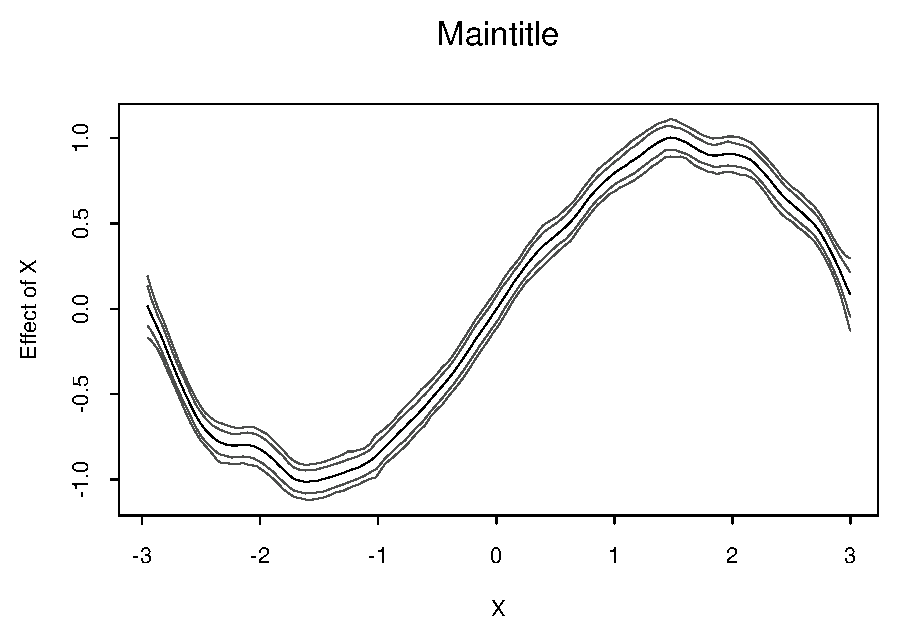
\includegraphics[scale=0.8]{grafiken/plotnonp.eps}
{\em\caption{ \label{illgraph} Illustration for the usage of
\em\tt plotnonp}}
\end{center}
\end{figure}

This statement draws the estimated effect of #X# and stores the
graph in the postscript file #"c:\\bayes\\reg_f_X_rw.ps"#. A
title, a x-axis and y-axis label are added to the graph. For
illustration purposes, the resulting graph is shown in
\autoref{illgraph}.

In some situations the effect of a covariate representing dates must
be plotted. Suppose for example that a covariate has values ranging
from 1 to 19 representing the time period from January 1983 to July
1984. In this case, we naturally prefer that the x-axis is labelled
in terms of dates rather than in the original coding (from 1 to 19).
To achieve this, function #plotnonp# provides the three additional
options #year#, #month# and #step#. Options #year# and #month# are
used to specify the year and the month (1 for January, 2 for
February, \dots) corresponding to the minimum covariate value. In
the example mentioned above #year=1983# and #month=1# will produce
the correct result. In addition, option #step# may be specified to
define the periodicity in which your data are collected. For example
#step=12# (the default) corresponds to monthly data, while #step=4#,
#step=2# and #step=1# correspond to quarterly, half yearly and
yearly data. We illustrate the usage of #year#, #month# and #step#
with our example. Suppose we estimated the effect of calendar time
#D#, say, on a certain dependent variable, where the range of the
data is as described above. Then the following function call will
produce the postscript file shown in \autoref{illgraph2}:

\begin{figure}[ht]
\begin{center}
%\includegraphics[scale=0.8]{fvdate.eps}
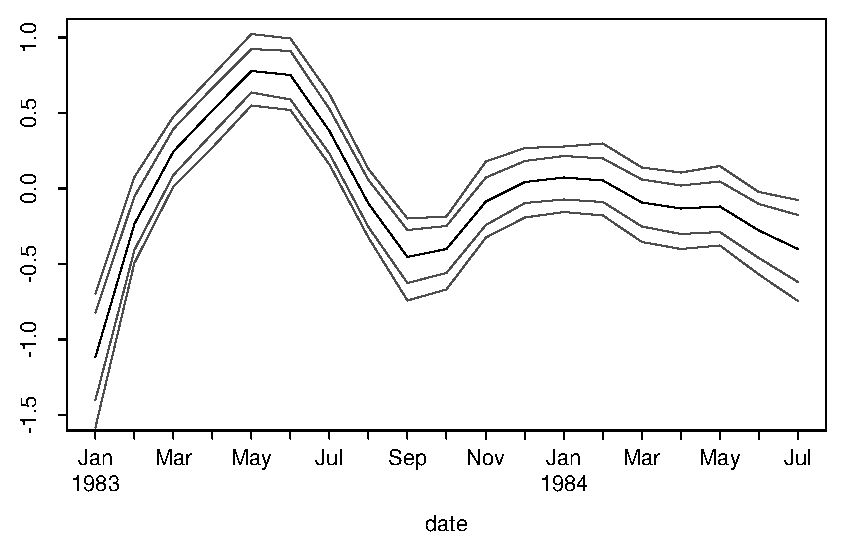
\includegraphics[scale=0.8]{grafiken/plotnonpdate.eps}
{\em\caption{ \label{illgraph2} Illustration for the usage of
\em\tt plotnonp}}
\end{center}
\end{figure}

#> plotnonp("c:\\bayes\\reg_f_D_pspline.res",psname="c:\\bayes\\reg_f_D_pspline.ps",#\\
#  year=1983,month=1,step=12,xlab="date",ylab= " ") #

Note, that \texttt{ylab=" "} forces R / S-plus to omit the y-axis
label. If #ylab# (as well as #xlab#) is omitted, default labels will
be given to the two axis.

Finally, we note that all options that can be passed to the #plot#
function of R / S-plus may also be passed to function #plotnonp#.
Thus, function #plotnonp# is more or less a specialized version of
the #plot# function.


\subsection{Drawing geographical maps} \index{S-plus!drawing
geographical maps} \index{R!drawing geographical maps}
\index{drawing geographical maps}

This subsection describes how to visualize estimation results of
spatial covariates, where the observations represent the location
or site in connected geographical regions. A typical example for a
spatial covariate is given in the 'rents for flats' example, see
\autoref{rentdata}, where the covariate #L# indicates the location
(in subquarters) of the flat in Munich. \autoref{munich} shows a
map of Munich separated into subquarters.

\begin{figure}
\centering
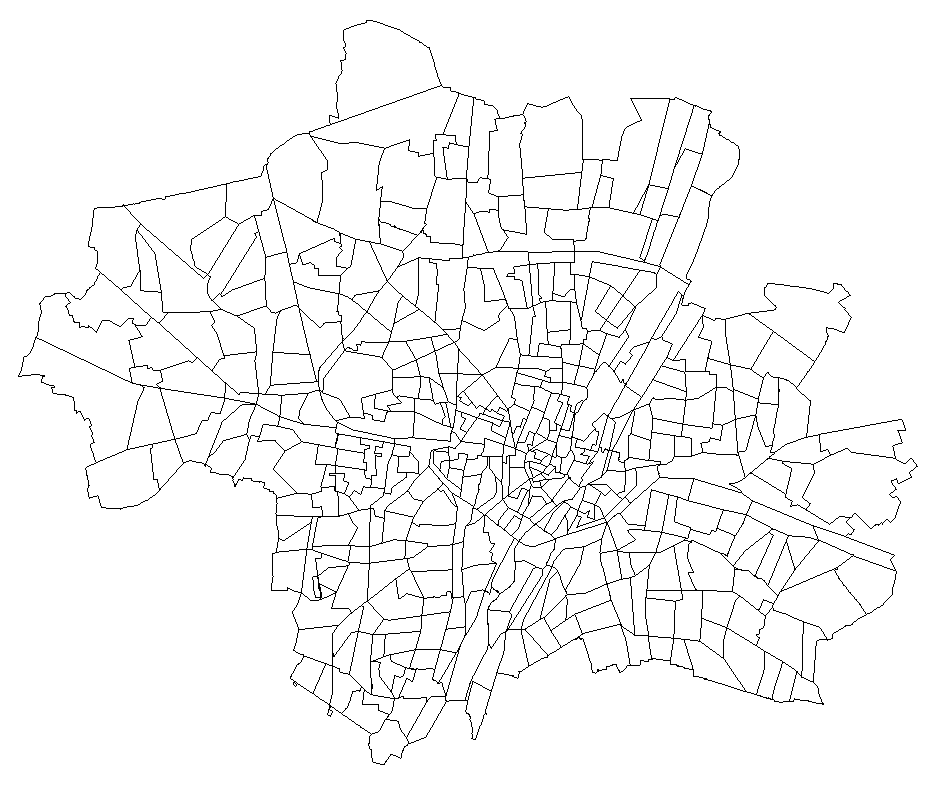
\includegraphics [scale=0.5]{grafiken/munich.eps}
{\em\caption{\label{munich} Map of Munich}}
\end{figure}


Typically, the effect of such a spatial covariate is incorporated
into a regression model via an unstructured or structured random
effect. In the latter case a spatial smoothness prior for the
spatial covariate is specified that penalizes too abrupt changes of
the estimated effect in neighboring sites. In some situations the
incorporation of both, an unstructured and a structured effect, may
also be appropriate. Details on how to incorporate spatial
covariates into a semiparametric regression  model are given in
\autoref{bayesregress} ({\em bayesreg objects}) and
\autoref{remlregregress} ({\em remlreg objects}). For the rest of
this section we assume that an effect of a spatial covariate has
already been estimated and that we now want to visualize the
estimation results. This can be easily done with the two functions
#readbndfile# and #drawmap#. Function #readbndfile# is used to read
the boundary information of a map that is stored in a so called
boundary file and to store this information as a permanent {\em map
object}. The boundary file contains mainly the polygons which form
the different geographical regions of the map. The required
structure of such a file is described below. After the successful
reading of the boundary information of a map, the second function
#drawmap# may be used to draw and print the map either on the screen
or into a postscript file. There are several possible ways to draw
the map. In the simplest case the map can be drawn without any
estimation effects, i.e.~only the boundaries of the different
regions or sites are drawn, see \autoref{munich} for an example. In
practice, however, one usually wants to color the regions of the map
according to some numerical characteristics. As an example compare
\autoref{munichrelfreq} in which the subquarters of Munich are
colored according to the frequency of flats in the 'rents for flats'
data set located in the respective subquarter. Subquarters colored
in red contain less flats compared to subquarters colored in green.
In striped areas no observations are available.

\begin{figure}[ht]
\begin{center}
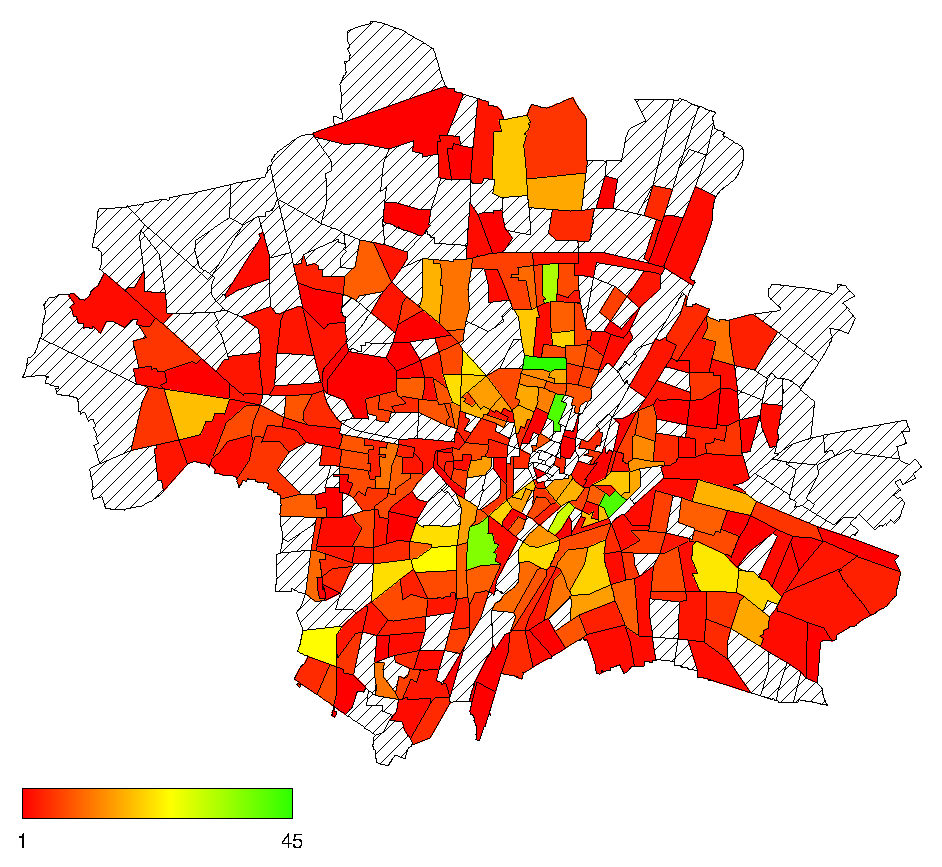
\includegraphics[scale=0.5]{grafiken/munichfr.eps}
{\em\caption{ \label{munichrelfreq} relative frequencies of
observed flats in the 'rents for flats' data set}}
\end{center}
\end{figure}


In the following we give a detailed description of the usage of
the functions #readbndfile# and #drawmap#.

\subsubsection*{Function readbndfile}
\index{R!reading boundary files} \index{S-plus!reading boundary
files} \index{reading boundary files}

Function #readbndfile# is used to read in boundary information
stored in a boundary file. The function has two required arguments.
The first argument is the filename of the boundary file to read in.
The second argument specifies the name of the {\em map object}
(recall that the map information is stored as a permanent object).
To give an example, suppose that {\em BayesX} is installed in the
directory #c:\bayes# and that we want to read in the map of Munich.
In this case the boundary file of the map is stored in the
subdirectory #examples# of the installation directory, that is in
#c:\bayes\examples#. The name of the boundary file is simply
#munich.bnd#. The following function call reads in the boundary
information of Munich and stores the map permanently in the object
#munich#:

#> readbndfile("c:\\bayes\\examples\\munich.bnd","munich")#

Once again, note that double backslashes are required to specify a
directory. The second argument in the statement above is "munich",
i.e.~the name of the map object is simply #munich#. To refer to the
map of Munich in subsequent statements and function calls, the
quotation marks must be omitted.

\subsubsection*{Function drawmap}
\index{S-plus!drawmap}\index{R!drawmap}

Function #drawmap# is used to draw geographical maps and color the
regions according to some numerical characteristics. There is only
one required argument that must be passed to #drawmap#, that is the
name of the map to be drawn. Provided that the map has already been
read into R / S-plus (via function #readbndfile#), the following
statement draws the map of Munich in a graphic-window on the screen:

#> drawmap(map=munich)#

Storing the map in a postscript file rather than drawing it on the
screen can be achieved by specifying the name of the postscript
file using the #outfile# option. For example the command

#> drawmap(map=munich,outfile="c:\\bayes\\munich.ps")#

produces a postscript file named #munich.ps# with the map of
Munich.

However, in most cases one not only wants to draw the boundaries of
a geographical map, but also color the regions according to some
numerical characteristics. Suppose for example that we have already
estimated a location specific effect on the monthly rents in the
'rents for flats' data set. Suppose further that the estimated
effects are stored in #c:\bayes\output\reg_f_L_spatial.res#. The
structure of the file is described in detail in
\autoref{bayesregress} ({\em bayesreg objects}) and
\autoref{remlregregress} ({\em remlreg objects}).

Suppose now that we want to visualize estimation results for the
spatial covariate #L# by coloring the subquarters of Munich
according to the posterior mean estimated using a {\em bayesreg
object}. Compared to the statement above, (at least) three more
arguments must be passed to function #drawmap#; the argument #dfile#
that specifies the filename of estimated results, the argument
#plotvar# that specifies the variable to be plotted and the argument
#regionvar# that specifies which column of the file, containing
estimation results, stores the region names. The following statement
produces the desired result:

 #> drawmap(map=munich,outfile="c:\\bayes\\munich.ps", #\\
 #  dfile="c:\\bayes\\output\\reg_f_L_spatial.res", plotvar="pmean",regionvar="L")#

Note that the right hand side of options #plotvar# and #regionvar#
must be enclosed by quotation marks. If we want to color the
subquarters of Munich according to the posterior mode estimated
using a {\em remlreg object} we have to change the statement to

 #> drawmap(map=munich,outfile="c:\\bayes\\munich.ps", #\\
 #  dfile="c:\\bayes\\output\\reg_f_L_spatial.res", plotvar="pmode",regionvar="L")#

\subsubsection*{Optional arguments of function drawmap}

Besides the arguments discussed so far there are some more
optional arguments that can be passed to #drawmap#. They are
listed and described below together with a summary of the
arguments already described:

\begin{itemize}
\item #cex.legend = #{\em realvalue}

This option is only available for the R-version of #drawmap#.
#cex.legend# specifies the  magnification to be used for legend
annotation. The default value is #cex.legend=0.7#.

\item #color = T#/#F#

The #color# option allows to choose between a grey scale for the
colors and a colored scale. The default is #color=F#, which means a
grey scale.

\item #dfile = "#{\em filename (including path)}#"#

Filename (including path) of the file containing numerical
characteristics of the regions of the map. The file must contain at
least two columns, one column that lists the names of the regions
and one column containing the numerical characteristics of the
respective regions. It is important that the names of the regions
listed match with the region names stored in the {\em map object}.
The first row of the file must contain the names of the columns.

\item #drawnames = T#/#F#

In some situations it may be favorable to print the names of the
regions into the graph (although the result may be confusing in most
cases). This can be done by specifying the additional option
#drawnames=T#. By default the names of the regions are omitted in
the graph.

\item #hcl = T#/#F#

This option is only available for the R-version of #drawmap# and
depends on the package #vcd#. Specifying #hcl=T# requests that a
color palette from the HCL color space should be used instead of an
RGB palette. The HCL colors will be selected diverging from a
neutral center (grey) to two different extreme colors (red and
green) in contrast to the RGB colors diverging from yellow to red
and green. HCL colors are particularly useful for electronic
presentations since they are device-independent. Option #hcl=T# is
only meaningful in combination with the option #color=T#.

\item #legend = T#/#F#

By default a legend is drawn into the graph. To omit the legend in
the graph, #legend=F# must be passed as an additional argument.

\item #lowerlimit = #{\em realvalue}

Lower limit of the range to be drawn. If #lowerlimit# is omitted,
the minimum numerical value in the #plotvar# column will be used
instead as the lower limit.

\item #map = "#{\em characterstring}#"#

Name of the {\em map object}. Use function #readbndfile# to read in
geographical maps.

\item #nrcolors = #{\em integer}

To color the regions according to their numerical characteristics,
the data are divided into a (typically large) number of ordered
categories. Afterwards a color is associated with each category. The
#nrcolors# option can be used to specify the number of categories
(and with it the number of different colors). Default value is 100.

\item #outfile = "#{\em filename (including path)}#"#

Filename (including path) of the postscript file where the map
should be stored.

\item #pcat = T#/#F#

If you want to visualize the values of the columns #pcat80# or
#pcat95# it is convenient to specify #pcat=T#. This forces #drawmap#
to expect a column that consists only of the values -1, 0 and 1. Of
course you can achieve the same result by setting #nrcolors=3#,
#lowerlimit=-1# and #upperlimit=1#. The default is #pcat=F#.

\item #plotvar = "#{\em characterstring}#"#

Name of the column in the data file containing the numerical
characteristics of the regions (see also argument #dfile#). Note
that the right hand side must be enclosed by quotation marks.

\item #pstitle = "#{\em characterstring}#"#

Adds a title to the graph. Note that the right hand side must be
enclosed by quotation marks.

\item #regionvar = "#{\em characterstring}#"#

Name of the column in the data file containing the region names
(see also argument #dfile#). Note that the right hand side must be
enclosed by quotation marks.

\item #swapcolors = T#/#F#

In some situations it may be favorable to swap the order of the
colors, i.e.~red shades corresponding to large values and green
shades corresponding to small values. This is achieved by specifying
#swapcolors=T#. By default small values are colored in red shades
and large values in green shades.

\item #upperlimit = #{\em realvalue}

Upper limit of the range to be drawn. If #upperlimit# is omitted,
the maximum numerical value in the #plotvar# column will be used
instead as the upper limit.

\end{itemize}

\subsection{Plotting two-dimensional surfaces}
\label{splusplotsurf} \index{S-plus!plotting two-dimensional
surfaces} \index{R!plotting two-dimensional surfaces}
\index{plotting two-dimensional surfaces}

This subsection describes the usage of the function #plotsurf# for
visualizing two-dimensional surfaces. The function #plotsurf#
merely invokes different R / S-plus functions for visualizing
two-dimensional data. Thus, users familiar with R / S-plus may
prefer to use this functions directly to gain more flexibility.

Suppose that a Bayesian regression model has already been
estimated with predictor

$$
\eta = \dots + f(X1,X2) + \dots,
$$

where the interaction effect of #X1# and #X2# is modelled
nonparametrically using two-dimensional P-splines and that the
estimation results are stored in file:

#c:\bayes\output\reg_f_X1_X2_pspline.res#

The function #plotsurf# requires at least one argument, which is the
name (including path) of the file containing the estimation results.
For example the command

#> plotsurf("c:\\bayes\\output\\reg_f_X1_X2_pspline.res")#

plots the estimated surface against #X1# and #X2# on the screen.
There are several additional options that can be passed, for
example for changing the plot type or storing the graph as a
postscript file rather than displaying it on the screen. The
following list describes all possible arguments that may be passed
to the function #plotsurf#:

\begin{itemize}
\item #cols = #{\em 3 column vector}

This option is only meaningful, if the argument #data# is specified.
In this case #cols# gives the columns of the object or data file
passed to the argument #data#, that should be used as values for the
x, y and z axis. The default is #cols=c(2,3,4)# which corresponds to
plotting the estimated surface against #X1# and #X2#.

\item #data = "#{\em filename (including path)}#"#

Name (including path) of the file containing the estimation
results. The file must contain at least 3 columns, one for the
x-axis, one for the y-axis and one for the z-axis. The file must
contain a header.

\item #mode = 1#/#2#/#3#/#4#/#5#

This option specifies the plot type. In S-Plus there are five
different types available, where the default value #mode=1#
corresponds to what is called a 'Surface Plot' in S-plus. In R three
different types are available corresponding to a perspective plot
(#mode=1#, function #persp# in R), a contour plot (#mode=2#,
function #contour# in R), and an image plot (#mode=2#, function
#image# in R) of the data. In R #plotsurf# depends on the package
#akima# for the interpolation of irregular data.

\item #outfile = "#{\em filename (including path)}#"#

Name (including path) of the postscript file where the graph
should be stored. This option is only meaningful for #mode=2# and
#mode=3#.

%\item {\bf zlim = 2 column vector}

%2 column vector giving the minimum and maximum value to be put on
%the z-axis.

\end{itemize}

\subsection{Plotting autocorrelation functions}
\label{splusplotautocor} \index{S-plus!plotting autocorrelation
functions} \index{R!plotting autocorrelation functions}
\index{plotting autocorrelation functions} \index{autocorrelation
functions!plotting}

This section describes how to visualize autocorrelation functions of
sampled parameters using the function #plotautocor#.

To compute autocorrelation functions, the post-estimation command
#autocor# must be applied, see \autoref{bayesautocorr} for
details. For the rest of this section we assume that
autocorrelations are already computed and stored in file:

#c:\bayes\output\reg_autocor.raw#

The minimum number of arguments required for the function is one,
namely the file where the computed autocorrelation functions are
stored. In this case a {\em graphic window} will be opened and the
autocorrelation functions are plotted on the screen. To store
autocorrelations in a postscript file, an output filename must be
specified as a second argument. Thus, the command

#> plotautocor("c:\\bayes\\output\\reg_autocor.raw")#

prints autocorrelations on the screen, while the statement

 #> plotautocor("c:\\bayes\\output\\reg_autocor.raw","c:\\bayes\\output\\reg_autocor.ps")#

forces R / S-plus to store the autocorrelation graphs in the
postscript file #c:\bayes\output\reg_autocor.ps#.

In particular for regression models with a large number of
parameters the execution of function #plotautocor# can be very time
consuming. Moreover, the size of the resulting postscript file can
be very large. To avoid such problems #plotautocor# provides the
additional argument #mean.autocor#. If #mean.autocor=T# is
specified, for each lag number and model term only minimum, mean and
maximum autocorrelations are plotted, leading in most cases to a
considerable reduction in computing time and storing size.

\subsection{Plotting sampled parameters} \label{splusplotsample}
\index{R!plotting sampled parameters}\index{S-plus!plotting sampled
parameters} \index{plotting sampled parameters}

This section describes how to plot sampled parameters using the
function #plotsample#. Before applying function #plotsample#,
sampled parameters must be stored in ASCII-format using the
post-estimation command #getsample#. See \autoref{bayesgetsample}
for details, but note that sampled parameters will be stored in
several different files, typically one file for each term in the
model.

Suppose now that we want to visualize sampling paths for the
parameters of the nonlinear effect of a covariate X. Assume
further that sampled parameters are stored in the ASCII file

#c:\bayes\output\reg_X_sample.raw#.

As most other functions, #plotsample# provides two possibilities
of drawing sampled parameters. The first possibility is to print
the graphs on the screen, and the second is to store them into a
postscript file. To print the sampling paths on the screen, only
the filename (including path) of the ASCII file where sampled
parameters are stored must be passed to the function. For the
example mentioned above the corresponding command is:

#> plotsample("c:\\bayes\\output\\reg_X_sample.raw")#

If sampling paths should be drawn into a postscript file rather
than on the screen, the filename of the resulting postscript file
must be specified as a second argument. Thus, for our example we
get:

 #> plotsample("c:\\bayes\\output\\reg_X_sample.raw","c:\\bayes\\output\\reg_X_sample.ps")#

In addition, all options that are available for the R / S-plus
function #plot# may be passed to function #plotsample#, see the
S-plus documentation for details.


\chapter{DAG Objects}
\index{Model selection} \index{Dag objects} \label{dag}

{\em Author: Eva--Maria Fronk} \\
\vspace{0.3cm}



%%%%%%%%%%%%%%%%%%%%%%%%%%%%%%%%%%%%%%%%%%%%%%%%%%%%%%%%%%%%%%%%%%%%%%%%%%%%%%%%%%%%%%%%%%%%%%%%%%%%%%%%%%%%%%%%%%%%%%%
Dag objects are needed to estimate dag models using reversible
jump MCMC. The considered variables may be Gaussian or binary,
even the mixed case of a conditional Gaussian distribution is
possible. A general introduction into graphical models can be
found in Lauritzen (1996). For a description of the more
particular Gaussian dags see for instance Geiger and Heckerman
(1994). We refer to Brooks (1998) or Gilks (1996) for an
introduction into MCMC simulation techniques. For the more general
reversible jump MCMC have a look at Green (1995); for reversible
jump MCMC in context of graphical models at Giudici and Green
(1999). The following explanations to the statistical background
of the program can be found in more detail in Fronk and Giudici
(2000).



\section{Method estimate}



\subsection{Description}

The method #estimate# estimates the dependency structure of the
given variable which is represented by a dag. Furthermore, the
parameters of this model are estimated. This is done within a
Bayesian framework; we assume prior distributions for the unknown
parameters and use MCMC techniques for estimation. In the
following we first focus on the Gaussian case  and describe the
statistical model which is assumed for the variables. Some
factorizations which result from the properties of dags are also
given. To represent the dags we rely on the concept of adjacency
matrices which is briefly explained and necessary to understand
the output. We finally give some brief information about the used
algorithm without going into details. Finally, we address the
situation of binary and mixed (i.e.~continuous and binary)
variables, too, which is reduced to the Gaussian case by
introducing latent variables.

\subsubsection*{Model Assumptions }
\index{Dag object!Assumptions}

A Gaussian dag $d$ can be represented as a regression model for
each variable $X_i, \, i=0, \dots, p-1$, given the parents of
$X_i$, denoted by $\X_{pa(i)}$,
%
\begin{eqnarray}
X_i \mid \x_{pa(i)},  \mbeta_{i \mid pa(i)}, \sigma_{i \mid
pa(i)}^2, d \sim  \N(\beta_{i0} + \sum_{x_l \in pa(x_i)}
\beta_{il}x_l, \sigma_{i \mid pa(i)}^2). \nonumber
\end{eqnarray}
%
The joint distribution of all variables ${\bf X} = (X_0, \dots,
X_{p-1})'$ is then given by
%
\begin{eqnarray}
%p(\x \mid  \mmu, \mSigma) =
p(\x \mid  \mbeta, \msigma^2) = \prod_{i=0}^{p-1} p(x_i \mid
\x_{pa(i)}, \mbeta_{i \mid pa(i)}, \sigma_{i \mid pa(i)}^2),
\nonumber
\end{eqnarray}
%
where $\mbeta_{i \mid pa(i)}$ is the $|pa(i)|+1$-dimensional
vector of the intercept $\beta_{i0}$ and the $|pa(i)|$ regression
coefficients of $X_i$. Furthermore, $\sigma_{i \mid pa(i)}^2$ is
the partial variance of $X_i$ given its parents $\x_{pa(i)}$. Let
$\mbeta = (\mbeta'_{0 \mid pa(1)}, \dots, \mbeta'_{p-1 \mid
pa(p)})'$ denote the vector of the $\mbeta_{i \mid pa(i)}$'s and
accordingly $\msigma^2 = (\sigma_{0 \mid pa(1)}^2, \dots,
\sigma_{p-1 \mid pa(p)}^2)'$ the vector of the conditional
variances $\sigma_{i \mid pa(i)}^2$.

\bigskip

The vector $\mbeta_{i \mid pa(i)}$ is assumed to be normally
distributed with mean $\mb_{i \mid pa(i)}$ and covariance matrix $
\frac{1}{\alpha_i} \sigma_{i \mid pa(i)}^2 \I $, where $\alpha_i$
is a known scaling factor. For the sake of simplicity, we shall
assume $\alpha_i=\alpha$. Formally:
%
$$\mbeta_{i \mid pa(i)} \mid \sigma_{i \mid pa(i)}^2, d   \sim
\N_{|pa(i)|+1} \left ( \mb_{i \mid pa(i)}, \,\frac{1}{\alpha}
\sigma_{i \mid pa(i)}^2 \I  \right ).$$
%
This implies that the coefficients of a regression model are
assumed to be mutually independent. For the partial variance
$\sigma_{i \mid pa(i)}^2$ we use an inverse gamma prior with
parameters $\delta_{i \mid pa(i)}$ and $\lambda_{i \mid pa(i)}$:
%
$$\sigma_{i \mid pa(i)}^2 \mid  d \sim \mbox{IG} \left ( \delta_{i
\mid pa(i)}, \,\lambda_{i \mid pa(i)} \right).$$
%
Finally, by supposing that there exist $D$ possible dags, which,
in the absence of subject-matter information, have all the same
probability, we get a discrete uniform distribution for $d$: $p(d)
=  1/D.$ Taking advantage of the well-known factorization property
of the joint distribution
\begin{eqnarray}
p(\x \mid \mbeta, \msigma^2, d) &=&  \prod_{i=0}^{p-1} p(x_i \mid
\x_{pa(i)}, \mbeta_{i \mid pa(i)}, \sigma_{i\mid pa(i)}^2)
\nonumber
\end{eqnarray}
and the "global parameter independences"
\begin{eqnarray}
p(\mbeta \mid  \msigma^2, d) &=& \prod_{i=0}^{p-1} p(\mbeta_{i
\mid pa(i)} \mid \msigma_{i \mid pa(i)}^2),  \nonumber \\ [0.1cm]
\mbox{and \hspace{1cm}} p( \msigma^2 \mid d) &=& \prod_{i=0}^{p-1}
p(\sigma_{i \mid pa(i)}^2) \nonumber
\end{eqnarray}
(for a detailed description see Geiger and Heckerman, 1999), we
get the joint distribution:
%
\begin{eqnarray}
\lefteqn{ p(\x, \mbeta, \msigma^2, d)  }  \nonumber \\  [0.3cm]
&=&   p(\x \mid \mbeta, \msigma^2, d) \,p(\mbeta \mid \msigma^2, d)  \, p( \msigma^2 \mid d)  \, p(d) \nonumber\\
&=&    \prod_{i=0}^{p-1} p( \x_i \mid \x_{pa(i)}, \mbeta_{i \mid
pa(i)}, \sigma^2_{i \mid pa(i)})
    \, \prod_{i=0}^{p-1} p(\mbeta_{i \mid pa(i)} \mid \sigma_{i \mid pa(i)}^2)  \nonumber  \\
& &  \, \prod_{i=0}^{p-1} p(\sigma_{i \mid pa(i)}^2) \, p(d)
\nonumber
\end{eqnarray}

%joint distribution
%Taking advantage of the well-known factorization property of the
%joint distribution in (\ref{modularity_1}) and the "global
%parameter independence" in (\ref{modularity_2}) and
%(\ref{modularity_3}) (for a detailed description see Geiger and
%Heckerman, 1999):
%
%\begin{eqnarray}
%p(\x \mid \mbeta, \msigma^2, d)
%&=&  \prod_{i=1}^p p(x_i \mid \x_{pa(i)}, \mbeta_{i \mid pa(i)}, \sigma_{i\mid pa(i)}^2), \label{modularity_1}  \\ [0.1cm]
%p(\mbeta \mid  \msigma^2, d)
%&=& \prod_{i=1}^p p(\mbeta_{i \mid pa(i)} \mid \msigma_{i \mid pa(i)}^2), \label{modularity_2}   \\ [0.1cm]
%p( \msigma^2 \mid d) &=&  \prod_{i=1}^p p(\sigma_{i \mid pa(i)}^2). \label{modularity_3}
%\end{eqnarray}

\newpage

\subsubsection*{Representation of DAGs }
\index{Dag object!Representation}

To represent dags we rely on the concept of adjacency matrices.
For a given graph ${\cal G} =(V,E)$ with $|V|=p$, the adjacency
matrix of ${\cal G}$ is defined as the $(p \times p)$-matrix $A$,
$[A]_{ij}=a_{ij}$, with
%
\begin{eqnarray} a_{ij} = \left \{
\begin{array} {l}
            1, \mbox{ if } (v_i,v_j) \in E \hspace*{1cm} \\
            0, \mbox{ if } (v_i,v_j) \not\in E. \hspace*{1cm}
            \end{array} \right. \nonumber
\end{eqnarray}
%
In general, all three types of graphs (undirected, directed and
chain graphs) can be uniquely represented by the corresponding
adjacency matrix. Note that regarding dags, as we do, the parents
of the vertex $i$ are indicated by the $i$-th column, while its
children are given in the $i$-th row. We use the representation
via adjacency matrices also to check the acyclicity of the graph.
For an illustration of this concept consider the graph in
\autoref{adja}.
%
%
\begin{figure}[ht]
\renewcommand{\baselinestretch}{1.0}
{\small \hspace*{2cm}
\parbox {3cm}
{ \setlength{\unitlength}{1cm}
\begin{picture}(3, 5)
\put(0.5,3.5) {\circle*{0.2}}
\put(0.6,3.8){\makebox(0,0)[l]{$x_1$}} \put(0.5,1.5)
{\circle*{0.2}} \put(0.6,1.4){\makebox(0,0)[tl] {$x_2$}}
\put(2.5,1.5){\circle*{0.2}} \put(2.6,1.4){\makebox(0,0)[tl]
{$x_3$}} \put(2.5,3.5) {\circle*{0.2}}
\put(2.6,3.8){\makebox(0,0)[l] {$x_4$}}
\put(0.5,3.3) {\vector(0,-1){1.6}}      %von x_1 nach x_2
\put(0.7,1.5) {\vector(1,0){1.6}}       %von x_2 nach x_3
\put(0.7,3.3) {\vector(1,-1){1.6}}      %von x_1 nach x_3
\put(2.5,1.7)   {\vector(0,1){1.6}}     %von x_3 nach x_4
\end{picture}
} \hspace{3cm}
\parbox {6cm}
{ $ A = \left( \begin{array} {cccc}
0&  1&  0&  0   \\
0&  0&  1&  0   \\
1&  0&  0&  1   \\
0&  0&  0&  0
\end{array}
\right )$
 }
\vspace{-1cm} {\em\caption{\label{adja}A directed acyclic graph
containing and the corresponding adjacency matrix $A$.}}}
\end{figure}

\subsubsection*{Reversible Jump Algorithm for Continuous Variables}
\index{Model selection!Gaussian variables}

We are not only interested in estimating the parameters for a
given dag $d$ but also want to learn about the structure of $d$
itself. So we need to construct a Markov chain which has $
\pi(d,\mmu, \mbeta, \msigma^2\mid \x)$ as its invariant
distribution. Changing the dag like adding or deleting a directed
edge implies also a changing in the dimension of the parameter
space. To deal with this situation we use a reversible jump
algorithm. Reversible jump MCMC was proposed and described by
Green (1995); it can be regarded as a generalization of the usual
MCMC and allows to sample simultaneously from parameter spaces of
different dimensions.

Our algorithm can be briefly summarized by the following moves,
which produce a Markov chain in the state space that is made up by
the vector of unknowns $(d,\mbeta,\msigma^2)$:
%
\begin{enumerate}
\item Updating the dag $d$ by adding, switching or deleting a
directed edge, remaining always in the class of directed acyclic
graphs. When adding or deleting an edge this move involves a
change in dimensionality of the parameter space.
\item Update  $\mbeta_{i\mid pa(i)}$, $i=0, \dots, p-1$.
\item Update $\sigma^2_{i\mid pa(i)}$, $i=0, \dots, p-1$.
\end{enumerate}
%
For a detailed explanation of the different steps in the
continuous case, see Fronk and Giudici (2000). For a
simplification of the oftentimes crucial switch step, see Fronk
(2002) and also the explanations of the option {\it switch} in
\autoref{switch_step}.

\newpage

\subsubsection*{Reversible Jump Algorithm for Binary Variables}
\index{Model selection!Binary variables}

Now we consider the situation of $p$ binary variables of which the
joint distribution is assumed to be multinomial. The influence to
a variable $X_i$ from its known parents $\x_{pa(i)}$ shall be
given by a probit model, i.e.~
\begin{eqnarray} \label{probit}
p_{i} \,=\,  E(X_{i} \mid \x_{pa(i)})
      \,=\,  \Phi (  \x_{pa(i)}'\mbeta_{i \mid pa(i)}, \sigma_{i \mid pa(i)}^2),
\end{eqnarray}
where $i=1, \dots , p$ and  $\Phi (\mu ,\sigma^2)$ denotes the cdf
of the normal distribution. This binary situation is reduced to
the continuous one by sampling a latent variable, a so-called
utility, $Z_i$ for each binary variable $X_i$. The general idea is
found in Albert and Chib (1993). Here, we first focus on the
situation that we are only interested in the main effects. I.e.~we
do not take any interactions into account although they now of
course can occur as we do not longer consider the Gaussian case.
The algorithm, which does not account for interactions, can be
briefly summarized as:
%
\begin{enumerate}
\item  For $X_i$, $i=0, \dots, p-1$, draw $Z_{i}$ from its full conditional
        $\N(\x_{pa(i)}' \mbeta_{i \mid pa(i)},1)$, which is truncated at the left by 0 if $x_{i}=1$
        and at the  right if $x_{i}=0$.
\item Add, delete, or switch a directed edge like in the Gaussian case, but take the utility $Z_i$ instead of
$X_i$ as response in $i$th regression model; the covariables
$\x_{pa(i)}$ of the $i$th model remain unchanged.
\item Update  $\mbeta_{i\mid pa(i)}$, $i=0, \dots, p-1$.
\item Update $\sigma^2_{i\mid pa(i)}$, $i=0, \dots, p-1$.
\end{enumerate}

To be able to take interactions into account, inside the algorithm
interactions are treated as own variables. Due to the enormous
complexity we restrict ourselves to two way interactions which
seem sufficient for most situations in practice. For details, see
Fronk (2002).

\subsubsection*{Reversible Jump Algorithm for Mixed Case}
\index{Model selection!Mixed case}

For the mixed case, we assume the considered continuous and binary
variables to follow a conditional Gaussian (CG) distribution. For
a general introduction we refer to Lauritzen (1996). The
univariate conditioned distribution of $f(x_i \mid \x_{pa(i)})$
are then CG regressions (see Lauritzen and Wermuth, 1989) and can
be represented by a normal regression resp.~a probit model with
mixed covariables.
\begin{enumerate}
\item For all variables $X_i$, $i=0, \dots, p-1$,
    \begin{enumerate}
       \item[] If $X_i$ is discrete,
            \begin{enumerate}
            \item[] For all observations $X_{ki}$, $k=1, \dots, n$,  \\
                    draw utility $Z_{ki}$ from full conditional $Z_{ki} \mid x_{ki}, \x_{k pa(i)} \mbeta_{i \mid pa(i)}$
            \end{enumerate}
    \end{enumerate}
\item Update $d$, i.e.~cancel, add, or switch the directed edge $X_j \rightarrow X_i$;
      thereby distinguish
    \begin{itemize}
    \item Response $X_i$ is continuous:
    \begin{enumerate}
     \item Take the algorithm for the Gaussian case, where now the covariables
            $pa(X_i)$ can be continuous or binary
     \end{enumerate}
    \item Response $X_i$ is discrete
     \begin{enumerate}
     \item Replace binary response $X_i$ by continuous utility $Z_i$
     \item Consider the new or vanishing interactions among the parents of
     $X_i$ and possibly~$X_j$, that can be pairwise discrete or mixed
     \item Carry out birth, death or switch step
     \end{enumerate}
    \end{itemize}
\item Update $\mbeta_{i\mid pa(i)}$, $i=0, \dots, p-1$.
\item Update $\sigma^2_{i\mid pa(i)}$, $i=0, \dots, p-1$.
\end{enumerate}
%
For detailed explanations, see again Fronk (2002).

\subsubsection*{Remark about Markov-equivalence}

Our algorithm does not take care about the so-called Markov
equivalence, which describes the fact that different dags can
represent the same statistical model. Equivalent dags can be
summarized to equivalent classes which again can be represented by
one single graph, the essential graph. Of course model selection
could be done in a more effective way if only the space of those
essential graphs would be considered. This will be a task of our
research in future. For more details concerning Markov-equivalence
we refer to papers of Andersson et al. (1997a, b) and Chickering
(1995).


%%%%%%%%%%%%%%%%%%%%%%%%%%%%%%%%%%%%%%%%%%%%%%%%%%%%%%%%%%%%%%%%%%%%%%%%%%%%%%%%%%%%%%%%%%%%%%%%%%%%%%%%%%%%%%%%%%%%%%%


%{\bf  \large Syntax}\\[0.3cm]

\subsection{Syntax}
%
\index{Dag object!Estimate command} \index{Dag object!Create}
%
The creation of objects has been described in general in
\autoref{createobject}; in the context of dag models the
corresponding dag object is created by:

\begin{center}
{\texttt{dag} {\em objectname}},\\
\end{center}

To perform a model selection as described above call:

\begin{center}
{{\em objectname}.\texttt{estimate} {\em variables} [\texttt{if}
{\em expression}], [{\em options}]\texttt{ using} {\em dataset} }
\bigskip
\end{center}

Then the method #estimate# estimates the dag for the variables
given in {\it variables} which have to be defined in {\it
dataset}. The parameters of the via the dag defined regression
models are also estimated. An if-statement may be specified to
analyze only a part of the data set, i.e.~only those observations
where {\it expression} is true. There are several facultative {\it
options} concerning the (start) parameters of the algorithm or the
kind of output at the end. They are listed in the next paragraphs.

%{\bf  \large Options}\\[0.3cm]
\subsection{Options}

\subsubsection*{Options for controlling MCMC simulations}

The following options correspond to those given on
\hyperref[mcmc_options]{page~\pageref*{mcmc_options}} and are
therefore only briefly explained.
\begin{itemize}
\item #burnin = #{\em b} \\
Changes the number of burnin iterations from 2000 to {\em b}; it is a positive integer number with $0<b<500001$.\\
DEFAULT:# burnin = 2000#
\item #iterations = #{\em i} \\
Changes the number of MCMC iterations from 52000 to {\em i}; it is a positive integer number with $0< i<10000000$.\\
DEFAULT: #iterations = 52000#
\item #step = #{\em s} \\
Changes the thinning parameter of MCMC iterations from 50 to {\em s}; it is a positive integer number with $0<s<1000$.\\
DEFAULT: #step = 50#
\end{itemize}

\subsubsection*{Options for initial values of algorithm}
\begin{itemize}
%\item priori\_sigma
\item {\bf\sffamily Changing hyperparameters of partial variances} \\
As already mentioned we assume $\sigma_{i \mid pa(i)}^2 \sim IG
(\delta_{i \mid pa(i)},\lambda_{i \mid pa(i)} )$ for $i=0, \dots,
p-1$. By the following two commands the values of the two
hyperparameters $\delta_{i \mid pa(i)}$ and $\lambda_{i \mid
pa(i)}$ can be freely chosen. If this is not done the default
values correspond to a non-informative gamma distribution.
\begin{itemize}
\item #delta = #{\em c} \\
    Specifies the first parameter of the inverse gamma distribution of the partial
    variances, $\delta_{i \mid pa(i)}$, is set equal to $d$. Otherwise it is equal to 1. The value
    {\em c} has to be of type realvalue with $0< c<20$.\\
    DEFAULT: #delta =  1#
\item #lambda = #{\em l}\\
    Specifies the second parameter of the inverse gamma distribution of the partial
    variances, $\lambda_{i \mid pa(i)}$, is set equal to $l$. Otherwise it is equal to 0.005.
    The value {\em d} has to be of type realvalue with $0< d <20$.\\
    DEFAULT: #lambda = 0.005#
\end{itemize}
\item {\bf\sffamily Choosing special graph to start from} \\
Usually the algorithm starts from the independent model, that
means from a dag without any edges. This can be changed by the
command
\begin{center}
#type = #0/1/2/3/4\\
DEFAULT: #type = 0#
\end{center}
where the different values have the following meanings:
\begin{itemize}
\item #type=0# \\
    Algorithm starts from an {\bf independent} model with no edges.
\item #type=1# \\
    Algorithm starts from a {\bf complete} model where all edges are directed
    from "lower" variables to "higher" ones, i.e.~$x_i \rightarrow x_j, \, \forall i<j$.
\item #type=2# \\
    Algorithm starts from a {\bf complete} model where all edges are directed
    from "higher" variables to "lower" ones, i.e.~$x_j \rightarrow x_i, \, \forall i<j$.
\item #type=3# \\
    Algorithm starts from a model where there is an edge from each variable to
    the next "higher" one, like a {\bf chain}, i.e.~$x_i \rightarrow x_j, \, \forall i=j+1$.
\item #type=4# \\
    Algorithm starts from a model where there is an edge from each variable to
    the next "lower" one, like a {\bf chain}, i.e.~$x_j \rightarrow x_i, \, \forall i=j+1$.
\end{itemize}
\end{itemize}

\subsubsection*{Options concerning the way of model selection}

\begin{itemize}
\item {\bf\sffamily Kind of switch step} \label{switch_step} \\
There are three ways how the switch step can be carried out in the
rj-algorithm. The first one is similar to the performance of a
birth or death step (i.e.~adding or deleting an edge): A proposal
is made and then accepted by its corresponding acceptance ratio.
As it may be very complicate to calculate a good proposal, a
simplification can be achieved by the consideration if the switch
step leads to an equivalent dag model. If this holds true, the
given and the proposed dag should be statistically
indistinguishable. The proposed dag can therefore be accepted with
probability 0.5. The kind of switch step can be chosen by the
command
\begin{center}
    #switch = normal#/#equi#/#mix#, \\
    \hspace*{-1.8cm}  DEFAULT: #switch = normal#
\end{center}
which differ in the following way:
\begin{itemize}
\item #switch=normal#\\
The switch step is carried out by proposing the new dag and
accepting it with the corresponding acceptance probability. The
transformation into equivalent model may occur very seldom and,
consequently, the acceptance ratio very low.
\item #switch=equi# \\
The switch step is only allowed if it results into an equivalent
model. In this case, it is performed with a probability of 0.5.
Transformations into a non-equivalent model can only occur by a
birth or death step.
\item #switch=mix#\\
This command causes a mixture of both procedures described above:
If the proposed switch step leads to an equivalent model it is
accepted with probability 0.5. If it results into a non-equivalent
model a proposal is made and accepted by the corresponding
acceptance ratio.
\end{itemize}
\item {\bf\sffamily Kind of distribution family / interactions }\\
There are three different types of data sets as they can consists
of continuous, binary, or mixed variables which results in the
assumption of a Gaussian, a multinomial, or a conditional Gaussian
distribution. Dependent on the kind of data set the rj-algorithm
for the model selection changes as described above.This can be
indicated by the optional command
\begin{center}
    #family = continuous#/#discrete#/#mixed#.\\
\end{center}
In the case that the model selection for a binary data set shall
be carried out accounting for interactions the command
\begin{center}
    #family = discrete_ia#\\
\end{center}
is needed instead of  #family = discrete#. In this case, a special
option concerning the output is given by the command #detail_ia#
which is explained below.
\item {\bf\sffamily Restriction to the search space}\\
It is possible to restrict the search space, i.e.~to state an
(missing) edge as fix or determinate the orientation of an edge.
This is done by writing the restrictions into a file {\em
restrict} which is then read by the command
\begin{center}
    #fix_file = #{\em path\_of\_restrict}\\
\end{center}
The restriction is then given by a $p \times p$ matrix that lies
under the path {\em path\_of\_restrict}. The matrix is allowed to
have three possible entries, namely  0,1, and 2 which have the
following meaning: An entry of 2 corresponds to no restriction of
the corresponding edge, it may occur or not. An entry of 1
indicates that this edge has to exist in each graph of the Markov
chain, whereas 0 denotes that the corresponding edge must not
occur.
\end{itemize}

\subsubsection*{Options concerning the output}
\begin{itemize}
\item {\bf\sffamily Estimated regression coefficients}\\
As already mentioned, the parameters of each regression model are
estimated in every iteration. Because of the fact that the
qualitative structure of the dag is usually of greater interest
than the quantitative estimations of the regression coefficients,
in the standard output these estimated parameters are omitted.
Nevertheless
\begin{center}
#print_dags#
\end{center}
gives the mean, the 10\%, 50\% and the 90\% quantile of every
parameter of all regression models.
%averaged over {\bf all} dags of the Markov chain.
As the model space for dags is very huge we abandon the
possibility to store the estimated values for each dag. To perform
the necessary calculation {\em BayesX} creates a temporary file
under the device {\em c:$\setminus\setminus$...}. For this
purpose, its important to ensure that a device with this name
exists. Otherwise the user has to provide an alternative path for
the storage file by the command
\begin{center}
#store_file = #{\em alternative\_path}
\end{center}
\item {\bf\sffamily Estimated coefficients of interactions}
\end{itemize}

\begin{itemize}
\item {\bf\sffamily Criteria for the listed models} \\
    As model selection for dags is performed in an extremely huge search space one might not want
    to get a list of all models which have been visited during MCMC estimation regardless of the
    relative frequency of their appearance. The option
    \begin{center}
    #print_models = all#/#prob#/#limit#/#normal#, \\
    \hspace*{-1.8cm}  DEFAULT: #print_models = normal#
    \end{center}
    %where "all", "prob" and  "limit" are strings,
    allows to focus
    on special criterions for the models printed in the output.
\begin{itemize}
\item #print_models = all#  \\
    All models which have been visited by the Markov chain are printed.
\item #print_models = prob# \\
    The most frequent models of the chain are printed except for those which are the less frequent
    ones and have altogether a probability of alpha=0.05. The value of alpha can be changed as
    it is explained a few lines below.
\item #print_models = limit# \\
    Here, the first 10 models with the highest frequencies are printed. The number of listed models
    can be made different from 10 as it is explained a few lines below.
\item #print_models = normal# \\
    The option #normal# is a mixture of #limit# and #prob#, as it chooses the one
    which produces less models. The default parameters are again alpha=0.05 and number=10.
\end{itemize}
The default setting of  #print_models# is #print_models=normal#.
\item #number = #{\em n} \\
    Changes the number of printed models in the option  #print_models = limit# to $n$.
    The variable number has to be of type realvalue with $0 \leq n \leq 10000$. \\
    DEFAULT = 10
\item #alpha = #{\em a} \\
    Sets alpha in the option {\tt print\_models = prob} equal to $a$. That means when using
    {\tt print\_models = prob} the most frequent models which unify 1-a  of the posterior
    probability are printed. The variable alpha has to be of type intvalue with $a \in [0,1]$. \\
    DEFAULT = 0.05
\item #printit = #{\em p} \\
    Prints every {\em p}-th iteration in the output window instead of every 100-th. The printing of the
    iterations can be suppressed by setting $p$ higher than the number of iterations. The variable printit has to be of
    type intvalue with $0 < p< 10000001$. \\
    DEFAULT = 100
\end{itemize}

%%%%%%%%%%%%%%%%%%%%%%%%%%%%%%%%%%%%%%%%%%%%%%%%%%%%%%%%%%%%%%%%%%%%%%%%%%%%%%%%%%%%%%%%%%%%%%%%%%%%%%%%%%%%%%%%%%%%%%%


%{\bf  \large Estimation Output}\\[0.3cm]
\subsection{Estimation Output}

The output can be written to a file by opening a logfile before
using the estimation command. It has to be closed afterwards. The
use of logfiles is described in detail in \autoref{logfile}. The
output itself is structured as follows:
\begin{itemize}
\item {\bf\sffamily Listing of different dags:}\\
The different models are listed by their adjacency matrices. In
order to save space, the different rows are printed in one line
with a blank indicating the beginning of a new one. The number of
edges is given as well as the absolute and relative frequency of
the model. For example the first line of the exemplifying output
in \autoref{output}
%
\begin{figure}
\begin{center}
{\it

Number of different dags visited by the algorithm: 16 \\[0.5cm]
******** DIFFERENT MODELS sorted by frequencies  ******** \\
********************** all models ********************** \\[0.2cm]

\begin{tabular}{llllll}
010 \hspace{0.2cm}& 000 \hspace{0.2cm}& 000 \hspace{0.5cm}&    1  \hspace{0.5cm}& 3894  \hspace{0.5cm}&  0.3890 \\
000 \hspace{0.2cm}& 100 \hspace{0.2cm}& 000 \hspace{0.5cm}&    1  \hspace{0.5cm}& 3814  \hspace{0.5cm}&  0.3810 \\
000 \hspace{0.2cm}& 100 \hspace{0.2cm}& 100 \hspace{0.5cm}&    2
\hspace{0.5cm}& \,\,806   \hspace{0.5cm}&  0.0806
\end{tabular}
}


$\vdots$ \\[-0.15cm]
$\vdots$

\end{center}
{\em\caption{\label{output} Example for model listing in the
output.}}
\end{figure}
%
gives the information that the most frequent model is represented
by the adjacency matrix $ A = \left( \begin{array} {cccc}
0&1&0   \\
0&0&0   \\
0&0&0
\end{array}
\right )$ and contains 1 edge. It occurred in the thinned out
Markov chain for 3894 times which corresponds to a relative
frequency of about 0.389. Notice, that different dags may
represent the same statistical model as they may be
Markov-equivalent.
%
%
\item {\bf\sffamily Listing of essential graphs}\\
\begin{figure}
%\begin{center}
{\it

Number of different equivalent classes visited by the algorithm: 6 \\[0.5cm]
******* DIFFERENT EQUIVALENCE CLASSES sorted by frequencies  ********\\
**************************** all models ******************************** \\[0.5cm]

Skeleton: 010 000 000\\
No immoralities.\\
Number of edges: 1 \hspace{0.3cm} Abs.freq.: 7708 \hspace{0.3cm} Rel.freq.: 0.771 \\[0.3cm]

Skeleton: 011 000 000 \\
Immoralities: (0;1,2) \\
Number of edges: 2 \hspace{0.3cm} Abs.freq.: 806 \hspace{0.3cm} Rel.freq.: 0.0806 \\[0.3cm]

Skeleton: 011 000 000 \\
No immoralities. \\
Number of edges: 2 \hspace{0.3cm} Abs.freq.: 523 \hspace{0.3cm} Rel.freq.: 0.0523\\

$\vdots$ \\[-0.15cm]
$\vdots$

}
%\end{center}
{\em\caption{\label{output_ess} Example for listing of equivalence
classes in the output.}}
\end{figure}
Additional to the dags, the essential graphs are printed, too.
I.e.~those dags, which are equivalent to each other, are
summarized and represented by their essential graph. The
representation of the essential graph, which can contain
undirected as well as directed edges, is as follows. First the
underlying graph, the skeleton, is given by the adjacency matrix
as described above. But now, the entries indicate always an
undirected edge. (E.g.~the undirected graph $a$--$b$ of the two
variables $a$ and $b$ is given by 01 00.) Then the immoralities of
the essential graph are listed. Remember that within an essential
graph an oriented edge can only occur as a part of an immorality
$b \rightarrow a \leftarrow c$ which is here represented by the
triple (a;b,c). The example output of Figure \autoref{output_ess}
shows that the first two dag models of \autoref{output} which are
equivalent have been summarized to their representing essential
graph $X_0$--$X_1$ $X_2$. The next most frequent statistical model
is represented by the essential graph $X_0 \rightarrow X_2
\leftarrow X_1$ which is given by our representation as the
skeleton matrix 011 000 000 and the immorality (0;1,2).
%
%
\item {\bf\sffamily Averaged adjacency matrix:}\\
The $(i,j)$-th element of the averaged adjacency matrix gives the
estimated posterior probability of the presence of the edge $i
\rightarrow j$ in the true dag.
\item {\bf\sffamily Mean of skeletons:}\\
The skeleton of a dag is defined as the same graph without
regarding the directions of the edges. Equivalent dags have at
least the same skeleton. So it may be helpful to have also a look
at the averaged matrix of the skeletons, which is of course
symmetric.
\item {\bf\sffamily Correlation:}\\
The marginal and the partial correlation matrices of the regarded
data set is given, too.
\item {\bf\sffamily Ratios:}\\
We give some short information about the acceptance ratios for the
birth-, death- and switch-steps which denotes the cases where an
edge is added, dropped or switched. The first two cases imply a
change in dimension and are therefore sampled by a reversible jump
step.
\item {\bf\sffamily Estimated parameters:}\\
If the option {\tt print\_dags} is used, the estimated regression
coefficients $\mbeta_{i \mid -i}$, $i=0, \dots, p-1$, are listed
at the end. The notation $-i$ denotes all variables except for
$i$. Besides the mean of the sampled Markov chain for each
parameter there is also the 10\%, the 50\% and the 90\% quantile
given. As in equivalent models the direction of edges and, thus,
also the regression models vary, in most cases the estimated
regression coefficients do not give a deeper insight into the
model and have to be interpreted in a very careful way.
%\item {\bf Estimated interactions:}\\
\end{itemize}

%%%%%%%%%%%%%%%%%%%%%%%%%%%%%%%%%%%%%%%%%%%%%%%%%%%%%%%%%%%%%%%%%%%%%%%%%%%%%%%%%%%%%%%%%%%%%%%%%%%%%%%%%%%%%%%%%%%%%%%
\subsection{References}

\begin{description}

{\small

\item [Andersson, S.~A., Madigan, D., and Perlman, M.~D.~(1997a).] A
Characterization of Markov equivalence Classes for Acyclic
Digraphs. {\it The Annals of Statistics}, {\bf 25}, 505--541.
%
\item[Andersson, S.~A., Madigan, D., and Perlman, M.~D.~(1997b).] On the
Markov equivalence of Chain Graphs, Undirected Graphs, and Acyclic
Digraphs. { \it Scandinavian Journal of Statistics}, {\bf  24},
81--102.

\item[Chickering, D.~M.~(1995).] A Transformational Characterization of Equivalent Bayesian Network Structures.
In P.~Besnard and S.~Hanks (Eds.), {\it Uncertainty in Artificial
Intelligence, Proceedings of the Eleventh Conference}, San
Francisco: Morgan Kaufmann, pp. 87 -- 98
%
\item[Brooks, S.~P.~(1998).] Markov Chain Monte Carlo Method and its Application. {\it The Statistician},
{\bf 47}, 69--100.
%
\item[Fronk, E.--M. and Giudici, P. (2000).] Markov Chain Monte Carlo model selection for DAG Models.
       {\it Discussion Paper}, Universit\"{a}t M\"{u}nchen.
%
%\item{Gelman, A., Carlin, J.~B., Stern, H.~S., and Rubin,
%D.~B.~(1995).} {\it Bayesian Data Analysis}, Chapman and Hall,
%London.
%
%
\item[Geiger, D. and Heckerman, D.~(1994).] Learning Gaussian Networks.
{\it Proceedings of the Tenth Conference on Uncertainty in
Artificial Intelligence.} Morgan Kaufmann, 235--243.
%
\item[Geiger, D. and Heckerman, D.~(1999).] Parameter priors for
directed acyclic graphical models and the characterisation of
several probability distributions. Submitted for publication.
%
\item [Gilks, W.~R., Richardson, S., and Spiegelhalter, D.~J. (1996).]
        {\it Markov Chain Monte Carlo in Practice.},Chapman and Hall, London.
%
\item[Giudici, P.~and Green, P.~J.~(1999).] Decomposable Graphical
Gaussian Model Determination. {\it Biometrika}, {\bf 86},
785--801.
%
%\item{Giudici, P., Green, P.~J., and Tarantola, C.~(1999).} Efficient
%Model Determination for Discrete Graphical Models. Submitted for
%publication.
%
\item [Green, P.~J.~(1995).]
Reversible Jump Markov Chain Monte Carlo Computation and Bayesian
Model Determination. {\it Biometrika}, {\bf  82}, 711--32.
%
\item[Lauritzen, S.~L.~(1996).] {\it Graphical Models}, Clarendon Press, Oxford.

%\item{Lang, S.~and Brezger, A.~(2000).} BayesX--Software for
%Bayesian Inference Based on Markov Chain Monte Carlo Simulation Techniques.
%Discussion Paper 187,
%Sonderforschungsbereich 386, Ludwig--Maximilians--Universit\"at, M\"unchen, Germany.
%
%\item{Schachter, R.~and Kenley, C.~(1989).} Gaussian Influence Diagrams.
%{\it Management Science}, {\bf 35}, 527--550.
}

\end{description}


%{\bf  \large Example}\\[0.3cm]
%\subsection{Example}
%Blablabla...  ist das notwendig ?????



\addcontentsline{toc}{chapter}{Index}
\documentclass[11pt,a4paper,twoside]{bayesxreport}


\usepackage{amsfonts}
\usepackage[dvips]{graphicx}
\usepackage[dvips]{epsfig}
\usepackage{fancyhdr}
\usepackage{dsfont}
\usepackage{amsmath}
\usepackage{dsfont}
\usepackage{amssymb}

%\usepackage{showkeys}
%\usepackage{showidx}

\usepackage{rotating}
\usepackage{shortvrb}
\usepackage{multicol}
\usepackage{longtable}
\usepackage{xr}

\usepackage[ps2pdf]{thumbpdf}
\usepackage[ps2pdf]{hyperref}

\input{prepictex}
\input{pictexwd}
\input{postpictex}

\hypersetup{
%    pdffitwindow=true,
    pdfstartview=FitB,
    pdftitle={BayesX Manuals},
    pdfauthor={Christiane Belitz, Andreas Brezger, Thomas Kneib, Stefan Lang and Nikolaus Umlauf},
    colorlinks=true,
    linkcolor=blue,
    pdfpagemode=UseOutlines,
    bookmarksopen=true,
    bookmarksnumbered=true,
    pdfstartpage={1},
    hyperindex=true
    }

\usepackage[dcu]{harvard}

\sloppy
\parindent0em
\parskip0.3em
\topmargin -0.3cm \textheight24cm \textwidth16.5cm \headheight0.5cm \oddsidemargin-0.4cm \evensidemargin-0.4cm

 \fancyhead[RO,LE]{\thepage}
 \fancyhead[C]{}
 \fancyhead[LO]{\nouppercase\rightmark}
 \fancyhead[RE]{\nouppercase\leftmark}
 \fancyfoot[RO,LE]{}
 \fancyfoot[C]{\small\today} %Am ende raus!!!
 \fancyfoot[LO,RE]{}
 \fancyfoot[C]{}

 \renewcommand{\headrulewidth}{.4pt}
 \renewcommand{\footrulewidth}{0pt} %Am Ende 0 !!!

\pagestyle{fancy}


\renewcommand{\descriptionlabel}[1]{\hspace\labelsep\sc #1}

 \newcommand{\Cov}{\mbox{Cov}}
 \newcommand{\diag}{\mbox{diag}}
 \newcommand{\trace}{\mbox{trace}}
 \newcommand{\df}{\mbox{df}}

\def \re {{\bf R}}
\def \beq {\begin{equation}}
\def \eeq {\end{equation}}
\def \bdis {\begin{displaymath}}
\def \edis {\end{displaymath}}
\def \ds {\displaystyle}

\def \mbeta {\mbox{\boldmath $\beta$}}
\def \mtheta {\mbox{\boldmath $\theta$}}
\def \hatmbeta {\mbox{\boldmath $\hat\beta$}}
\def \eps {\epsilon}
\def \meps {\mbox{\boldmath $\epsilon$}}
\def \mmu {\mbox{\boldmath $\mu$}}
\def \mnu {\mbox{\boldmath $\nu$}}
\def \mSigma {\mbox{\boldmath $\Sigma$}}
\def \mGamma {\mbox{\boldmath $\Gamma$}}
\def \msigma {\mbox{\boldmath $\sigma$}}
\def \mPhi {\mbox{\boldmath $\Phi$}}
\def \Sigmavec {\mbox{\boldmath $\Sigma$}}
\def \sigmavec {\mbox{\boldmath $\sigma$}}
\def \nuvec {\mbox{\boldmath $\nu$}}
\def \tauvec {\mbox{\boldmath $\tau$}}




\newcommand{\N}{\mbox{N}}
\newcommand{\Var}{\mbox{Var}}
\newcommand{\E}{\mbox{E}}

\newcommand{\X}{\mbox{\boldmath $X$}}
\newcommand{\x}{\xvec}
\newcommand{\Z}{\mbox{\boldmath $Z$}}
\newcommand{\z}{\mbox{\boldmath $z$}}
\newcommand{\mb}{\mbox{\boldmath $b$}}
\newcommand{\Fx}{\mbox{\scriptsize \boldmath $x$}}
\newcommand{\I}{\mbox{\boldmath $I$}}
\newcommand{\Y}{\mbox{\boldmath $Y$}}
\newcommand{\y}{\mbox{\boldmath $y$}}
\newcommand{\mS}{\mbox{\boldmath $S$}}
\newcommand{\T}{\mbox{\boldmath $T$}}
\newcommand{\K}{\mbox{\boldmath $K$}}
\newcommand{\kt}{\mbox{\boldmath $t$}}
\newcommand{\U}{\mbox{\boldmath $U$}}
\newcommand{\fu}{\mbox{\boldmath $u$}}
\newcommand{\ba}{\mbox{\boldmath $\alpha$}}
\newcommand{\bb}{\mbox{\boldmath $\beta$}}

\def \Mvec {\vec{M}}
\def \Kvec {\vec{K}}
\def \mM {\vec{M}}
\def \Pvec {\vec{P}}
\def \Svec {\vec{S}}
\def \deltavec {\vec{\delta}}
\def \lambdavec {\boldsymbol{\lambda}}
\def \Lambdavec {\boldsymbol{\Lambda}}
\def \betavec {\boldsymbol{\beta}}
\def \etavec {\boldsymbol{\eta}}
\def \gammavec {\boldsymbol{\gamma}}
\def \Gammavec {\boldsymbol{\Gamma}}
\def \Omegavec {\boldsymbol{\Omega}}
\def \muvec {\boldsymbol{\mu}}
\def \kappavec {\boldsymbol{\kappa}}
\def \nuvec {\boldsymbol{\nu}}
\def \pivec {\vec{\pi}}
\def \thetavec {\vec{\theta}}
\def \varthetavec{\vec{\vartheta}}
\def \varepsilonvec {\boldsymbol{\varepsilon}}
\def \zetavec {\vec{\zeta}}
\def \Sigmavec {\boldsymbol{\Sigma}}
\def \Thetavec {\boldsymbol{\theta}}

\def \dvec {\mathbf{d}}
\def \fvec {\mathbf{f}}
\def \fhatvec {\mathbf{\hat{f}}}
\def \svec {\mathbf{s}}
\def \wvec {\mathbf{w}}
\def \xvec {\mathbf{x}}
\def \yvec {\mathbf{y}}
\def \uvec {\mathbf{u}}
\def \avec {\mathbf{a}}
\def \zvec {\mathbf{z}}
\def \bvec {\mathbf{b}}
\def \tvec {\mathbf{t}}
\def \mvec {\mathbf{m}}
\def \cvec {\mathbf{c}}

\def \ds {\displaystyle}

\def \Gvec {\mathbf{G}}
\def \Rvec {\mathbf{R}}
\def \Avec {\mathbf{A}}
\def \Bvec {\mathbf{B}}
\def \Cvec {\mathbf{C}}
\def \Dvec {\mathbf{D}}
\def \Fvec {\mathbf{F}}
\def \Kvec {\mathbf{K}}
\def \Hvec {\mathbf{H}}
\def \Ivec {\mathbf{I}}
\def \Lvec {\mathbf{L}}
\def \Uvec {\mathbf{U}}
\def \Wvec {\mathbf{W}}
\def \Yvec {\mathbf{Y}}
\def \Zvec {\mathbf{Z}}
\def \svec {\mathbf{s}}
\def \Cvec {\mathbf{C}}
\def \dvec {\mathbf{d}}
\def \Avec {\mathbf{A}}
\def \Pvec {\mathbf{P}}
\def \Vvec {\mathbf{V}}
\def \xivec {\mathbf{x_i}}
\def \xjvec {\mathbf{x_j}}
\def \betavecr {\vec{\beta_r}}
\def \betavec {\boldsymbol{\beta}}
\def \betadach {\hat{\vec{\beta}}}
\def \betadachr {\vec{\hat{\beta}_r}}
\def \betaschl {\vec{\tilde{\beta}}}
\def \betaschlr {\vec{\tilde{\beta}_r}}
\def \sschlr {\vec{\tilde{s}_r}}
\def \Aschlr {\vec{\tilde{A}_r}}
\def \Adach {\vec{\hat{A}}}
\def \Avecr {\vec{A}_r}
\def \Adachr {\vec{\hat{A}_r}}
\def \Fdach {\vec{\hat{F}}}
\def \Vdach {\vec{\hat{V}}}
\def \Aschl {\vec{\tilde{A}}}
\def \Xvec {\mathbf{X}}

\def \nullvec {\boldsymbol{0}}

\def \hvec {\vec{h}}
\def \vvec {\vec{v}}
\def \wvec {\vec{w}}
\def \x1vec {\vec{x_1}}
\def \xnvec {\vec{x_n}}

\def \Kmat {\mathbf{K}}
\def \Kmatj {\mathbf{K}_j}
\def \Xmat {\mathbf{X}}
\def \Vmat {\mathbf{V}}
\def \Smat {\mathbf{S}}


\def \dsR {\text{$\mathds{R}$}}
 \DeclareMathOperator{\B}{B}

\def \einsvec {\boldsymbol{1}}

\newcommand{\subheader}[1]{\textsf{\textbf{{\large #1}}}}

\newenvironment{stanza}[2]{\subheader{#1} \begin{itemize} \item[]#2}{\end{itemize}}


\newcommand{\preface}[1]{
\thispagestyle{empty}

\begin{center}
{\bf \em \huge BayesX}

\vspace{0.5cm}

{\em \large Software for Bayesian Inference in Structured Additive Regression Models}

\vspace{0.5cm}

{\em Version 2.1}

\vspace{0.5cm}

\begin{figure}[h]
\begin{center}
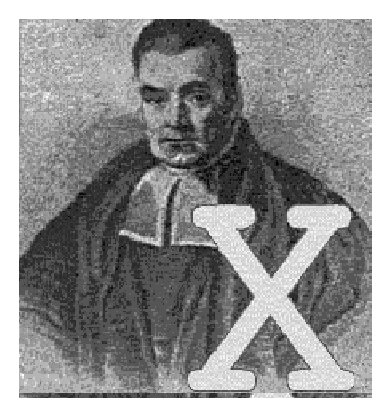
\includegraphics[scale=1.2]{grafiken/bayesicon.eps}
\end{center}
\end{figure}

\vfill

{\bf\sffamily \huge #1}

\vfill

\end{center}

{\em Developed by}

Christiane Belitz\\
Andreas Brezger\\
Thomas Kneib (University of G{\"o}ttingen)\\
Stefan Lang (University of Innsbruck) \\
Nikolaus Umlauf (University of Innsbruck) \\

\vspace{2ex}

{\em With contributions by}

\vspace{-1.5ex}

\begin{multicols}{2}
Daniel Adler
Eva-Maria Fronk\\
Felix Heinzl\\
Andrea Hennerfeind\\
Manuela Hummel\\
Alexander Jerak\\
Susanne Konrath\\
Petra Kragler\\
Cornelia Oberhauser\\
Leyre Est\'{\i}baliz Osuna Echavarr\'{\i}a\\
Daniel Saban\'{e}s Bov\'{e} \\
Achim Zeileis
\end{multicols}

{\em Supported by}

Ludwig Fahrmeir (mentally)\\
Leo Held (mentally)\\
German Research Foundation (DFG)

\newpage

\subsection*{Acknowledgements}

The development of {\em BayesX} has been supported by grants from the German Research Foundation (DFG), Collaborative
Research Center 386 ``Statistical Analysis of Discrete Structures''.

Special thanks go to (in alphabetical order of first names):

{\em Dieter Gollnow} for computing and providing the map of Munich (a really hard job); \\
{\em Leo Held} for advertising the program; \\
{\em Ludwig Fahrmeir} for his patience with finishing the program and for carefully
reading and correcting the  manual; \\
{\em Ngianga-Bakwin Kandala} for being the first user of the program (a really hard job); \\
{\em Samson Babatunde Adebayo} for carefully reading and correcting the manual; \\
{\em Ursula Becker} for carefully reading and correcting the manual;

\subsection*{Licensing agreement}

This program is free software; you can redistribute it and/or
modify it under the terms of the GNU General Public License
as published by the Free Software Foundation; either version 2
of the License, or (at your option) any later version.

This program is distributed in the hope that it will be useful,
but WITHOUT ANY WARRANTY; without even the implied warranty of
MERCHANTABILITY or FITNESS FOR A PARTICULAR PURPOSE.  See the
GNU General Public License for more details.

You should have received a copy of the GNU General Public License
along with this program; if not, write to the Free Software
Foundation, Inc., 51 Franklin Street, Fifth Floor, Boston, MA  02110-1301, USA.



\vspace{0.5cm}

{\em BayesX} is available at { \href{http://www.bayesx.org}{http://www.bayesx.org}}}


 \externaldocument{manual_star}
 \externaldocument{manual_tutorials}

\makeindex

\setcounter{secnumdepth}{3}

\begin{document}
\MakeShortVerb{\#}

\preface{Reference Manual}

\pdfbookmark[1]{Contents}{contents} \tableofcontents \hypertarget{contents}{}

\newpage

\chapter{What is BayesX?}

{\em BayesX} is a software tool for performing complex Bayesian
inference. The main features of {\em BayesX} are:
\begin{itemize}
\item {\bf Bayesian semiparametric regression based on MCMC simulation techniques} \\
{\em BayesX} provides a powerful regression tool for analyzing
regression and survival models with {\em structured additive
predictor} (STAR). STAR models cover a number of well known model
classes as special cases, e.g. {\em generalized additive models},
{\em generalized additive mixed models}, {\em geoadditive models},
{\em dynamic models}, {\em varying coefficient models}, and {\em
geographically weighted regression}. {\em BayesX} is able to
estimate nonlinear effects of continuous covariates, trends and
flexible seasonal patterns of time scales, correlated and/or
uncorrelated spatial effects (of geographical data) and
unstructured i.i.d. Gaussian effects of unordered group
indicators. The regression tool  supports the most common
distributions for the response variable. Supported distributions
for univariate responses are Gaussian, binomial, Poisson, negative
binomial and gamma. For multicategorial responses, both
multinomial logit or probit models for ordered categories of the
responses as well as cumulative threshold models for unordered
categories may be estimated. Recently complex models for
continuous time survival analysis based on the Cox model have been
added. At least some basic knowledge about Bayesian inference with
MCMC techniques is strongly recommended if you are interested in
using this tool. Details can be found in \autoref{star} and
\autoref{bayesreg}.
\item {\bf Inference for STAR models based on methodology for mixed models} \\
{\em BayesX} provides a second regression tool for estimating STAR
models with comparable functionality as the first tool based on
MCMC. This tool represents STAR models as {\em variance components
mixed models}. Inference is then based on estimation procedures
for mixed models, particularly {\em restricted maximum likelihood}
(REML). From a Bayesian perspective this yields empirical Bayes or
posterior mode estimates. Details can be found in \autoref{star}
and \autoref{remlreg}.
\item {\bf Model selection for Gaussian and non-Gaussian dag's} \\
This tool estimates Gaussian and non-Gaussian directed acyclical
graphs (dag) via reversible jump MCMC. Details are given in
\autoref{dag}
\item {\bf Handling and manipulation of data sets} \\
{\em BayesX} provides a growing number of functions for handling
and manipulating data sets, e.g. for reading ASCII data sets,
creating new variables, obtaining summary statistics etc. Details
are given in \autoref{datasetobj}.
\item {\bf Handling and manipulation of geographical maps} \\
{\em BayesX} is able to manipulate and draw geographical maps. The
regions of the map may be colored according to some numerical
characteristics. For details compare \autoref{map} and
\autoref{graphobj}.
\item {\bf Visualizing data} \\
{\em BayesX} provides functions for drawing scatter plots and
geographical maps. A number of additional options are provided to
customize the graphs according to the personal needs of the user.
Details can be found in \autoref{graphobj}.
\end{itemize}

\vspace{0.5cm} {\bf Recommendations for further reading}

\vspace{0.2cm} If you are interested in using {\em BayesX} it is
not necessary to read the complete manual. \autoref{recomm}
provides a guideline for reading this manual and other sources
depending on your purpose and background. In any case, you should
read \autoref{availableversions}-\autoref{generalusage} of
\autoref{gettingstarted} to make yourself familiar with {\em
BayesX}.


\begin{table}[ht] \footnotesize
\begin{center}
\begin{tabular}{ |p{7cm}|p{8.5cm}|}
\hline
{\bf Intended use and background} & {\bf Guideline} \\
\hline\hline Bayesian semiparametric regression based on MCMC
simulation techniques. No experience with MCMC techniques. & Read
first an introductory text about MCMC. A nice introduction is
given e.g. in Green (2001). Read \autoref{star} to make yourself
familiar with STAR regression models.
Proceed then with the tutorial like \autoref{zambiaanalysis} of \autoref{bayesreg}. \\
\hline Bayesian semiparametric regression based on MCMC simulation
techniques. At least a basic knowledge about MCMC techniques
exists. & Read \autoref{star} to make yourself familiar
with STAR regression models. Proceed then with the tutorial like \autoref{zambiaanalysis} of \autoref{bayesreg}. \\
\hline Semiparametric regression based on mixed model methodology.
& Read \autoref{star} to make yourself familiar with STAR
regression models. Proceed then with the tutorial like
\autoref{remlregzambianalysis} of \autoref{remlreg}. \\
\hline Model selection for dag's. No experience with reversible
jump MCMC. & Read first an introductory text about reversible jump
MCMC. A nice introduction is
given e.g. in Green (2001). Proceed with \autoref{dag}. \\
\hline
Draw and color geographical maps & Read \autoref{map} and \autoref{graphdrawmap} of \autoref{graphobj}. \\
\hline
\end{tabular}
{\em \caption {\label{recomm} Recommendations for further
reading}}
\end{center}
\end{table}

\subsubsection*{References}

\begin{description}
\item[Green, P.J. (2001):] A Primer in Markov Chain Monte Carlo. In: Barndorff-Nielsen, O.E.,
Cox, D.R. and Kl{\"u}ppelberg, C. (eds.), {\em Complex Stochastic
Systems}. Chapman and Hall, London, 1-62.
\end{description}


\chapter{Getting started}
\label{gettingstarted}

This chapter provides some useful information for first-time users
of {\em BayesX}: Which versions of BayesX are currently available
(\autoref{availableversions}), how is BayesX installed
(\autoref{installbayesx}), what types of manuals exist
(\autoref{bayesxmanuals}), and how is the graphical user interface
organized (\autoref{bayesxwindows}). Section \ref{generalusage}
describes the general usage of {\em BayesX} and the structure of
{\em BayesX} syntax. The final section contains a description of
three data sets that will be used for demonstrating purposes in
the later chapters.

\section{Available versions of BayesX}
\label{availableversions} \index{Java based version} \index{Non-Java
based version} \index{Versions} \index{Versions!Java based}
\index{Versions!Non-Java based}

In its current form, {\em BayesX} runs only under the various
versions of the Windows operating system (e.g. Windows 95, 98,
2000, NT, XP). The graphical user interface and the visualisation
tools are implemented in Java, while the computerintensive parts
of the program have been implemented in C++. The current version
of {\em BayesX} can be downloaded from
\href{http://www.stat.uni-muenchen.de/~bayesx}
{http://www.stat.uni-muenchen.de/\~{}bayesx}.

Up to version 1.3, {\em BayesX} has been distributed in two
versions, the {\em Java based version} described above and a {\em
non-Java based version}, which was written completely in C++.
Since the Java based version has additional features, the non-Java
based version is no longer supported.

\section{Installing BayesX}\label{installbayesx}
\index{Installation} \index{Installation directories}

After you have downloaded the file #installBayesX.exe# from the
{\em BayesX} homepage, proceed by executing this file. The
installation process is quite simple and comparable to most
standard installations. The installation routine will request all
necessary information.

When {\em BayesX} has been installed successfully, it can be
started using the {\em Windows Start} button or the icon created
on the desktop (depending on your specifications during the
installation process). The installation directory contains the
five subdirectories #doc#, #examples#, #output#, #sfunctions# and
#temp#. The #doc# directory contains the program documentation,
i.e. the three {\em BayesX} manuals (see the following
subsection). The #examples# directory contains the three data
sets, #credit.raw#, #rents.raw# and #zambia.raw#, which will be
used for demonstrating purposes throughout the manual. A detailed
description of these data sets is given in
\autoref{datadescription}. The #examples# directory also contains
some tutorial programs that illustrate the usage of {\em BayesX},
see the tutorials manual. The #output# directory is the default
directory for program output stored in files. Of course, the
output window can be redefined by the user, compare
\autoref{bayesregglobopt} and \autoref{remlregglobopt}. The
#sfunctions# directory contains some R and S-plus functions for
visualizing estimation results obtained with {\em bayesreg
objects} or {\em remlreg objects}, see \autoref{splus} for a
detailed description of these functions. Note, however, that the
current {\em BayesX} version has its own graphics capabilities,
see \autoref{graphobj} and \autoref{visualization} for details.
Finally, temporary files created when estimating regression models
will be stored in the #temp# directory. Usually you will never use
this directory.

The subdirectories and their content are briefly summarized in
\autoref{dirtable}.

\begin{table}[ht]
\begin{center}
\begin{tabular}{|l|l|}
\hline
Directory & Content \\
\hline
#doc# & the {\em BayesX} manuals \\
#examples# & data set examples and tutorial programs \\
#output# & default directory for estimation output \\
#sfunctions# & R and S-plus functions for visualizing output \\
#temp# & temporary files \\
\hline
\end{tabular}
{\em\caption{ \label{dirtable} Subdirectories of the installation
directory and their content.}}
\end{center}
\end{table}

\section{Manuals}\label{bayesxmanuals}
\index{Manuals}

{\em BayesX} is shipped with three different manuals. The
reference manual (i.e. the manual you are just reading) gives
detailed information on the general usage of BayesX, the syntax of
{\em BayesX} commands and the different objects used by {\em
BayesX}. The methodology manual provides background information on
the statistical methodology that is implemented in {\em BayesX}.
In this manual you will also find more references on the
methodological background. The tutorial manual is intended to make
new users familiar with the usage of {\em BayesX} by demonstrating
examples. It contains two self-contained tutorials, describing how
to perform semiparametric regression analyses using {\em BayesX}.
The manuals are also available from the help menu and can be found
in the #doc# directory (a subdirectory of the installation
directory).

\section{Windows and buttons in BayesX}\label{bayesxwindows}
\index{Windows}

After starting {\em BayesX} you will see a main window with a menu
bar and four additional subwindows. The four windows are the {\em
command window}, the {\em output window}, the {\em review window}
and the {\em object browser}. The purpose of these windows is
described in the following four subsections. Below the menu bar
there is a menu bar containing the buttons BREAK, PAUSE and
SUPPRESS OUTPUT, and the priority menu. Their functionality is
described in subsection \ref{buttons} and \ref{prioritymenu}.

\subsection{The command window}
\index{Command window} \index{Windows!Command}

Allmost all {\em BayesX} commands are entered and executed in the
{\em command window}. By default, a command will be executed if
you press the return key. You can change this default delimiter
using the #delimiter# command, see \autoref{delimiter}.

\subsection{The output window}
\index{Output window} \index{Windows!Output}

In the {\em output window}, all commands entered in the {\em
command window} or executed through a batch file (see
\autoref{batch}) are printed together with the program output.

\index{Saving the output} The content of the {\em output window} can
be saved and processed with your favorite text editor. For saving
the output, enter the {\em file menu} and click on {\em Save output}
or {\em Save output as}. The file save dialog will allow you to
choose between two different file formats. The default is the
rich-text format but it is also possible to store the {\em output
window} in plain ASCII format. This, however, has the disadvantage
that all text highlights (for example bold letters) will disappear
in the saved file.

The {\em file menu} also allows to clear the {\em output window}
(i.e. delete the content of the window) or to open an already
existing file.

Depending on the screen resolution of your computer, letters
appearing in the {\em output window} may be very small or too
large. The font size can be varied in the {\em preferences menu}.

\subsection{The review window}
\index{Review window} \index{Windows!Review}

In many cases, subsequent commands change only slightly. The {\em
review window} gives you convenient access to the last 100 past
commands entered during a session. Double click on one of these
past commands and it is automatically copied to the {\em command
window}, where it can be modified and / or executed again.

\subsection{The object browser}
\index{Object browser}

{\em BayesX} is object oriented, i.e. different types of objects
are used to store data, estimate regression models, etc. The {\em
object browser} provides an overview of the objects currently
defined and about their contents. The {\em object browser} window
is split into two parts. The left part displays the different
object types currently supported by {\em BayesX} ({\em dataset
objects}, {\em bayesreg objects}, {\em remlreg objects}, {\em map
objects}, {\em dag objects} and {\em graph objects})s. By clicking
on one of the object types, the names of all objects of this type
will appear in the right panel of the {\em object browser}. Double
clicking on one of the names gives a visualization of the object
and / or a short summary in the {\em output window}, depending on
the object type. Double clicking on {\em dataset objects}, for
example, will open a spreadsheet where the variables and the
observations of the data set can be inspected. Clicking on {\em
map objects} opens a window that contains a graphical
representation of the map.

\subsection{BREAK, PAUSE and SUPPRESS OUTPUT button}
\label{buttons} \index{PAUSE button} \index{BREAK button}
\index{SUPPRESS OUTPUT button} \index{Buttons} \index{Buttons!PAUSE}
\index{Buttons!BREAK} \index{Buttons!SUPPRESS OUTPUT}

The {\em BayesX} button panel contains the BREAK button, the PAUSE
button and the SUPPRESS OUTPUT button. The purpose of the BREAK
button is to interrupt the process that is currently executed
(this may take some time). Clicking on the PAUSE button interrupts
the current process temporarily until the button is pressed again.
If a process is paused, the button caption PAUSE is replaced by
CONTINUE, indicating that a second click on the button will
continue the current process. Pausing a current process will
increase the execution speed of other programs currently running
on your computer. Clicking the SUPPRESS OUTPUT button suppresses
printing of output in the {\em output window}. The button caption
changes to SHOW OUTPUT to indicate that an additional click on the
button will cause the program to print the output again.
Suppressing the output increases the execution speed of {\em
BayesX} and saves memory. Note, that you can store your output in
a log-file even if printing of the output is suppressed (see
\autoref{logfile}).

\subsection{Priority menu}
\label{prioritymenu} \index{Priority menu}

When running extensive computations, it may be desirable to reduce
the priority of BayesX since otherwise all further programs may be
executed very slowly. The priority menu allows you to change the
priority of your computations from within BayesX. Usually there
should be no need to increase the priority (although it is
possible). To pause the current computations use the PAUSE button.

\section{General usage of BayesX}
\label{generalusage}

\subsection{Creating objects}
\label{createobject} \index{Objects} \index{Objects!Create}

{\em BayesX} is implemented in an object oriented way, although
the object oriented concept does not go too far, i.e. inheritance
or other concepts of object oriented programming languages such as
S or C++ are not supported. As a consequence, the first thing to
do during a session, is to create some objects. Currently, six
different object types are available: {\em dataset objects}, {\em
bayesreg objects}, {\em remlreg objects}, {\em map objects}, {\em
dag objects} and {\em graph objects}. {\em Dataset objects} are
used to store, handle, and manipulate data sets, see
\autoref{datasetobj} for details. {\em Map objects} are used to
handle geographical information and are covered in more detail in
\autoref{map}. The main purpose of {\em map objects} is to serve
as auxiliary objects for {\em bayesreg objects} or {\em remlreg
objects} when estimating spatial effects. {\em Graph objects} are
used to visualize data (e.g. to create scatterplots or to color
geographical maps according to some numerical characteristics),
see \autoref{graphobj} for details. The most important object
types are {\em bayesreg objects} and {\em remlreg objects}. These
objects are used to estimate Bayesian semiparametric regression
models based on either Markov Chain Monte Carlo simulation
techniques ({\em bayesreg objects}) or a mixed model
representation of the regression model ({\em remlreg objects}).
See \autoref{bayesreg} for a detailed description of {\em bayesreg
objects} and \autoref{remlreg} for a detailed description of {\em
remlreg objects}. {\em Dag objects} are used to estimate Gaussian
or non-Gaussian DAGs (direct acyclic graphs) based on reversible
jump MCMC simulation techniques (see \autoref{dag} for details).

The syntax for creating a new object is:

#># {\em objecttype objectname}

To create for example a {\em dataset object} with name #mydata#, simply type:

#> dataset mydata#

Note that some restrictions are imposed on the names of objects,
i.e. not all object names are allowed. For example, object names
have to begin with an uppercase or lowercase letter rather than a
number. Section \ref{varnames} discusses valid variable names but
the same rules apply also to object names.

\subsection{Applying methods to previously defined objects}

When an object has been created successfully, you can apply methods
to that particular object. For instance, {\em dataset objects} may
be used to read data stored in an ASCII file using method #infile#,
to create new variables using method #generate#, to modify existing
variables using method #replace# and so on. The syntax for applying
methods to the objects is similar for all methods and independent of
the particular object type. The general syntax is: \index{General
syntax} \index{Syntax}

#># {\em objectname.methodname} [{\em model}] [#weight# {\em varname}] [#if# {\em boolean expression}] [, {\em options}] \\
\hspace*{4.8cm} [#using# {\em usingtext}]

\autoref{syntaxtable} explains the syntax parts in more detail.


\begin{table}[ht]
 \centering
\begin{tabular}{|l|l|}
\hline
Syntax part & Description \\
\hline
{\em objectname} & the name of the object to apply the method to \\
{\em methodname} & the name of the method \\
{\em model} & a model specification (for example a regression model) \\
{\em #weight# varname} & specifies {\em varname} as weight variable \\
#if# {\em boolean expression} & indicates that the method should be applied only if a \\
& certain condition holds \\
, {\em options} & define (or modify) options for the method \\
#using# {\em usingtext} & indicates that another object or file is required to \\
& apply the particular method \\
\hline
\end{tabular}
{\em \caption{\label{syntaxtable}Parts of the general BayesX
syntax.}}
\end{table}

Note that $[\dots]$ indicates that this part of the syntax is
optional and may be omitted. Moreover for most methods only some
of the syntax parts above will be meaningful. The specification of
invalid syntax parts is not allowed and will cause an error
message.

We illustrate the concept with some simple methods of {\em dataset
objects}. Suppose that a {\em dataset object} with name #mydata#
has already been created and that some variables should be
created. First of all, we have to tell {\em BayesX} how many
observations we want to create. This can be done with the
 #set obs# command, see also \autoref{setobs}. For example

#> mydata.set obs = 1000#

indicates that the data set #mydata# should have 1000
observations. In this case, the {\em methodname} is #set# and the
{\em model} is #obs =# #1000#. Since no other syntax parts (for
example #if# statements) are meaningful for this method, they are
not allowed. For instance, specifying an additional weight
variable #x# by typing

#> mydata.set obs = 1000 weight x#

will cause the error message:

#ERROR: weight statement not allowed#

In a second step we can now create a new variable #X#, say, that
contains Gaussian (pseudo) random numbers with mean 2 and standard
deviation 0.5:

#> mydata.generate X = 2+0.5*normal()#

Here, #generate# is the {\em methodname} and #X = 2+0.5*normal()#
is the {\em model}. In this case the {\em model} consists of the
specification of the new variable name, followed by the equal sign
'#=#' and a mathematical expression for the new variable. Similar
as for the #set obs# command other syntax parts are not meaningful
and therefore not allowed. If the negative values of #X# should be
replaced with the constant 0, this can be achieved using the
#replace# command:

#> mydata.replace X = 0 if X < 0#

Obviously, the #if# statement is meaningful and is therefore
allowed, but not required.

\section{Description of data set examples}
\label{datadescription} \index{Data set examples}

This section describes three data sets used to illustrate many of
the features of {\em BayesX} in the following chapters as well as
in the tutorial manual. All data sets are stored columnwise in
plain ASCII-format. The first row of each data set contains the
variable names separated by blanks. Subsequent rows contain the
observations, one observation per row.

\subsection{Rents for flats}
\label{rentdata} \index{Rents for flats} \index{Data set
examples!Rents for flats}

According to the German rental law, owners of apartments or flats
can base an increase in the amount that they charge for rent on
'average rents' for flats comparable in type, size, equipment,
quality and location in a community. To provide information about
these 'average rents', most of the larger cities publish 'rental
guides', which can be based on regression analyses with rent as
the dependent variable. The file #rent94.raw# (stored in the
#examples# directory) is a subsample of data collected in 1994 for
the Munich rental guide. The variable of primary interest is the
monthly rent per square meter in German Marks. Covariates
characterizing the flat were constructed from almost 200 variables
out of a questionnaire answered by tenants of flats. The present
data set contains a small subset of these variables that are
sufficient for demonstration purposes (see \autoref{rentdatavar}).

In addition to the data set, the #examples# directory contains a
map of Munich in the file #munich.bnd#. This map will be useful
for visualizing effects of the location #L#. See \autoref{map} for
a description on how to incorporate geographical maps into {\em
BayesX}.

\begin{table}

\centering
\begin{tabular}{|l|l|}
\hline
{\bf Variable} & {\bf Description} \\
\hline
R & monthly rent per square meter in German marks \\
$F$ & floor space in square meters \\
$A$ & year of construction \\
$L$ & location of the building in subquarters \\
 \hline
\end{tabular}
{\em \caption{\label{rentdatavar}Variables of the rent data set.}}
\end{table}


\subsubsection*{References}

\begin{description}

\item[Lang, S. and Brezger, A. (2004):]
\href{http://www.stat.uni-muenchen.de/~lang/publications.html}
{Bayesian P-splines.} {\it Journal of Computational and Graphical
Statistics}, 13, 183-212.

\end{description}


\subsection{Credit scoring}
\label{creditdata} \index{Credit scoring} \index{Data set
examples!Credit scoring}

The aim of credit scoring is to model and / or predict the
probability that a client with certain covariates ('risk factors')
will not pay back his credit. The data set contained in the file
#credit.raw# consists of 1000 consumer credits from a bank in
southern Germany. The response variable is 'creditability' in
dichotomous form ($y=0$ for creditworthy, $y=1$ for not
creditworthy). In addition, 20 covariates that are assumed to
influence creditability were collected. The present data set
(stored in the #examples# directory) contains a subset of these
covariates that proved to be the main influential variables on the
response variable, see Fahrmeir and Tutz (2001, ch. 2.1).
\autoref{creditdatavar} gives a description of the variables of
the data set. Usually a binary logit model is applied to estimate
the effect of the covariates on the probability of being not
creditworthy. As in the case of the rents for flats example, this
data set is used to demonstrate the usage of certain features of
{\em BayesX}, see primarily \autoref{creditanalyse} for a Bayesian
regression analysis of the data set.

\begin{table}[ht]

\begin{tabular}{|l|l|}
\hline
{\bf Variable} & {\bf Description} \\
\hline
$y$ & creditability, dichotomous with $y=0$ for creditworthy, $y=1$ for \\
    & not creditworthy \\
$account$ & running account, trichotomous with categories "no
running account" \\& ($=1$),
    "good running account"
($=2$),  "medium running account" \\&("less than 200 DM") ($=3$)  \\
$duration$ & duration of credit in months, continuous \\
$amount$ & amount of credit in 1000 DM, continuous \\
$payment$ & payment of previous credits, dichotomous with categories "good" ($=1$), \\ & "bad" ($=2$)  \\
$intuse$ & intended use, dichotomous with categories "private" ($=1$) or \\ & "professional" ($=2$)  \\
$marstat$ & marital status, with categories "married" ($=1$) and "living alone" ($=2$). \\
\hline
\end{tabular}
{\em \caption{\label{creditdatavar}Variables of the credit scoring
data set.}}
\end{table}

\subsubsection*{References}

\begin{description}
\item [Fahrmeir, L., Tutz, G. (2001):] {\it Multivariate Statistical
Modelling based on Generalized Linear Models.} New York:
Springer--Verlag.
\end{description}

\subsection{Childhood undernutrition in Zambia}
\label{zambia} \index{Childhood undernutrition} \index{Data set
examples!Childhood undernutrition}

Acute and chronic undernutrition is considered to be one of the
worst health problems in developing countries. Undernutrition
among children is usually determined by assessing the
anthropometric status of the child relative to a reference
standard. In our example undernutrition is measured through
stunting (insufficient height for age), indicating chronic
undernutrition. Stunting for child $i$ is determined using the
Z-score
\[Z_i = \frac{AI_i-MAI}{\sigma}\]
where $AI$ refers to the child`s anthropometric indicator (height
at a certain age in our example), MAI refers to the median of the
reference population and $\sigma$ refers to the standard deviation
of the reference population.

The data set #zambia.raw# contains the (standardized) Z-score for
4847 children together with several covariates that are supposed
to influence undernutrition (e.g. the body mass index of the
mother, the age of the child, and the district the mother lives
in). \autoref{zambiavar} gives more information on the covariates
in the data set.

This data set is used in chapter \ref*{zambiaanalysis} and
\ref*{remlregzambiaanalysis} of the tutorial manual.

\begin{table}[|h|t|]
\begin{center}
\begin{tabular}{|l|l|}
 \hline
 {\bf Variable} & {\bf Description}\\
 \hline
 $hazstd$ & standardized Z-score for stunting\\
 $bmi$ & body mass index of the mother\\
 $agc$ & age of the child\\
 $district$ & district where the mother lives\\
 $rcw$ & mother`s employment status with categories "working" (= 1) and "not working" \\
 & (= $-1$)\\
 $edu1$ & mother`s educational status with categories "complete primary but incomplete\\
 $edu2$ & secondary" ($edu1=1$), "complete secondary or higher" ($edu2=1$) and\\
 & "no education or incomplete primary" ($edu1=edu2=-1$)\\
 $tpr$ & locality of the domicile with categories "urban" (= 1) and "rural" (= $-1$)\\
 $sex$ & gender of the child with categories "male" (= 1) and
 "female" (= $-1$)\\
 \hline
\end{tabular}
{\em\caption{Variables in the undernutrition data set.
\label{zambiavar}}}
\end{center}
\end{table}

\subsubsection*{References}

\begin{description}
\item [Kandala, N. B., Lang, S., Klasen, S. and Fahrmeir, L. (2001):] Semiparametric Analysis of
the Socio-Demographic and Spatial Determinants of Undernutrition
in Two African Countries.{\it Research in Official Statistics}, 1,
81-100.
\end{description}


\chapter{Special Commands}

This chapter describes some commands that are not connected with a
particular object type. Among others, there are commands for
exiting {\em BayesX}, opening and closing log files, saving
program output, dropping objects etc..

\section{Exiting BayesX}
\index{exiting BayesX}

You can exit {\em BayesX} by simply typing either

#> exit#

or

#> quit#

in the {\em command window}.

\section{Opening and closing log files} \label{logfile}
\index{log files}

In a log file, program output and commands entered by the user,
are stored in plain ASCII format. This makes it easy to further
use the program output, for example results of statistical
procedures, in your favorite text editor. Another important
application of log files is
the documentation of your work. You open a log file by typing:

#> logopen# [{\em, option}] #using# {\em filename}

This opens a log file that will be saved in {\em filename}. After
opening a log file, all commands entered and all program output
appearing on the screen will be saved in this file. If the
log file specified in  {\em filename} is already existing, new
output is appended at the end of the file. To overwrite an
existing log file option #replace# must be specified in addition.
Note that it is not allowed to open more than one log file
simultaneously.

An open log file can be closed by simply typing:

#> logclose#

Note that exiting {\em BayesX} automatically closes the currently
open logfile.

\section{Saving the contents of the output window}
\index{output window!saving the contents} \index{saveoutput}

You can save the contents of the {\em output window} not only with
the {\em file-$>$save output} or {\em file-$>$save output as}
menu, but also using the #saveoutput# command. Saving the {\em
output window} with the #saveoutput# command is  particularly
useful in batch files, see \autoref{batch}. The syntax for saving
the
{\em output window} is

#> saveoutput# [{\em , options}] #using# {\em filename}

where {\em filename} is the file (including path) in which the
contents of the output will be saved.


\subsection*{Options}

\begin{itemize}
\item {\bf replace} \\
By default, an error will be raised if one tries to store the
contents of the {\em output window} in a file that is already
existing. This preserves you from overwriting a file
unintentionally. An already existing file can be overwritten by
explicitly specifying the #replace# option.
\item {\bf type = rtf $|$ txt } \\
The {\em output window} can be saved under two different file
types. By default, the contents of the window will be saved in
rich-text format. The second possibility is to store the {\em
output window} in plain ASCII--format. This can be done by
specifying #type = txt#. To explicitly store the file in rich-text
format {\em #type = rtf#} must be specified. \\
DEFAULT: #type = rtf#
\end{itemize}

\section{Changing the delimiter}
\label{delimiter} \index{delimiter}

By default, commands entered using the {\em command window} will
be executed by pressing the return key. This can be inconvenient,
in particular if your statements are long. In that case it may be
more favorable to split a statement into several lines, and
execute the command using a different delimiter than the return
key. You can change the delimiter using the #delimiter# command. The syntax is

#> delimiter# = {\em newdel}

where {\em newdel} is the new delimiter. There are only two
different delimiters allowed, namely the
return key and the ';' (semicolon) key. To specify the ';' key as the delimiter, type

#> delimiter = ;#

and press return. To return to the return key as the delimiter, type

#> delimiter = return;#

Note that the above statement must end with a semicolon, since
this was previously set to the current delimiter.


\section{Using batch files}
\label{batch} \index{batch files}

You can execute commands stored in a file just as if they were
entered from the keyboard. This may be useful if you want to
re-run a certain analysis more than once (possibly with some minor
changes) or if you want to run time consuming statistical methods
such as Bayesian regression based on MCMC simulation techniques
(see \autoref{bayesreg}).
You can run such batch files by simply typing

#> usefile# {\em filename}

This executes the commands stored in {\em filename} successively.
{\em BayesX} will not stop the execution if an error occurs in one
or more commands. Note that it is allowed to invoke
another batch file within a batch file currently running.


{\bf Comments}\index{comments}

Comments in batch files are allowed and are indicated by a  #%#
sign, that is every line
starting with a #%# sign is ignored by the program.

{\bf Changing the delimiter}

In particular in batch files, the readability of your program code
may be improved if some (long) commands are split up into several
lines. Normally this will cause errors, because {\em BayesX}
interprets each line in your program as one statement. To overcome
this problem one simply
has to change the delimiter using the #delimiter# command, see \autoref{delimiter}.


\section{Dropping objects}
\index{objects!dropping} \index{dropping objects}

You can delete objects by typing

#> drop# {\em objectlist}

This drops the objects specified in {\em objectlist}. The names of
the objects in {\em objectlist} must be separated by blanks.


\chapter{dataset objects} \label{chap_data}
\label{datasetobj} \index{dataset objects} \index{dataset}


{\em Dataset objects} are used to manage and manipulate data. A new {\em dataset object} is created by typing

#> dataset# {\em objectname}

where {\em objectname} is the name of the data set. After the
creation of a {\em dataset object} you can apply the methods for
manipulating and managing data sets discussed below.

Note that in the current version of {\em BayesX} {\bf only
numerical variables are allowed}. Hence, string valued variables,
for example,  are not yet supported by {\em BayesX}.



\clearpage



\section{Method descriptive}
\label{descriptive} \index{summary statistics}
\index{descriptives} \index{dataset!descriptive command}

\begin{stanza}{Description}

{Method #descriptive# calculates and displays univariate summary
statistics. The method computes the number of observations, the
mean, median, standard deviation, minimum and maximum of
variables.}
\end{stanza}

\begin{stanza}{Syntax}

{#> #{\em objectname}.#descriptive# {\em varlist} [#if# {\em expression}]

Method #descriptive# computes summary statistics for the variables
in {\em varlist}. An optional #if# statement may be added to
analyze only a part of the data.}
\end{stanza}

\begin{stanza}{Options}

{not allowed}
\end{stanza}


\begin{stanza}{Example}

{The statement

#> d.descriptive x y#

computes summary statistics for the variables #x# and #y#.
The statement

#> d.descriptive x y if x>0#

restricts the analysis to observations with #x>0#.}
\end{stanza}

\clearpage

\section{Method drop}
\label{drop} \index{dropping variables} \index{dropping
observations} \index{dataset!drop command}

%\bigskip
%{\bf \em  Description} \\

\begin{stanza}{Description}

{Method #drop# deletes variables or observations from the data set.}
\end{stanza}

%\bigskip
\begin{stanza}{Syntax}

{#> #{\em objectname}.#drop# {\em varlist}

#> #{\em objectname}.#drop if# {\em expression}

The first command may be used to eliminate the variables specified
in {\em varlist} from the data set. The second statement may be
used to eliminate certain observations. An observation will be
removed from the data set if {\em expression} is true.}
\end{stanza}


\begin{stanza}{Options}

{not allowed}
\end{stanza}


\begin{stanza}{Example}

The statement

#> credit.drop account duration#

drops the variables #account# and #duration# from the credit scoring data set. With the statement

#> credit.drop if marstat = 2#

all observations with #marstat = 2#, i.e. all persons living
alone, will be dropped from the credit scoring data set. The
following statement

#> credit.drop account duration if marstat = 2#

will raise the error

#ERROR: dropping variables and observations in one step not allowed#

It is not allowed to drop variables and certain observations in
one single command.
\end{stanza}



\clearpage



\section{Functions and Expressions}
\label{expression} \index{expressions}

The primary use of expressions is to generate new variables or
change existing variables, see \autoref{generate} and
\autoref{replace}, respectively. Expressions may also be used in
#if# statements to force {\em BayesX} to apply a method only to
observations where the boolean expression in the #if# statement
is true. The following are all examples of expressions:

#2+2# \\
#log(amount)# \\
#1*(age <= 30)+2*(age > 30 & age <= 40)+3*(age > 40)# \\
#age=30# \\
#age+3.4*age^2+2*age^3# \\
#amount/1000#


\subsection{Operators}
\index{expressions!operators} \index{operators}


{\em BayesX} knows three different types of operators: arithmetic,
relational and logical. Each of the types is discussed below.

\subsubsection{Arithmetic operators}
\index{operators!arithmetic}

The arithmetic operators are #+# (addition), #-# (subtraction),
#*# (multiplication), #/# (division), #^# (raise to a power) and
the prefix #-# (negation). Any arithmetic operation on a missing
value or an impossible arithmetic operation (such as division by
zero) yields a missing value.\\

\begin{stanza}{Example}

The expression

#(x+y^(3-x))/(x*y)#

denotes the formula

$$
\frac{x+y^{3-x}}{x\cdot y}
$$

and evaluates to missing if #x# or #y# is missing or zero.
\end{stanza}

\subsubsection{Relational operators}
\index{operators!relational}

The relational operators are #># (greater than), #<# (less than),
#>=# (greater than or equal), #<=# (less than or equal), #=#
(equal) and #!=# (not equal). Relational expressions are either 1
(i.e. the expression is true) or 0 (i.e. the expression is
false).\\

\begin{stanza}{Example}

Relational operators may be used to create indicator variables.
The following statement generates a new variable #amountcat# (out
of the already existing variable #amount#), whose
value is 1 if #amount<=10# and 2 if #amount>10#.

#> credit.generate amountcat = 1*(amount<=10)+2*(amount>10)#

Another useful application of relational operators is in #if#
statements. For example, changing
an existing variable only when a certain condition holds can be done by the following command:

#> credit.replace amount = NA if amount <= 0#

This sets all observations missing where #amount<=0#.
\end{stanza}

\subsubsection{Logical operators}
\index{operators!logical}

The logical operators are #&# (and) and #|# (or).

\subsubsection*{Example}

Suppose you want to generate a variable #amountind# whose value is
1 for married people with
amount greater than 10 and 0 otherwise. This can be done by typing

#> credit.generate amountind = 1*(marstat=1 & amount > 10)#

\subsubsection{Order of evaluation of the operators}
\index{operators!order of evaluation}

The order of evaluation (from first to last) of operators is

#^# \\
#/#, #*#\\
#-#, #+#\\
#!=#, #>#, #<#, #<=#, #>=#, #=#\\
#&#, #|#.

Brackets may be used to change the order of evaluation.


\subsection{Functions}
\index{functions}

Functions may appear in expressions. Functions are indicated by
the function name, an opening and a closing parenthesis. Inside
the parentheses one or more arguments may be specified. The
argument(s) of a function may be any expression, including other
functions. Multiple arguments are separated by commas. All
functions return missing values when given missing values as
arguments or when the result is undefined.

\autoref{mathfunc} references all mathematical functions;
\autoref{statfunc} references all statistical functions.
\index{functions!abs} \index{functions!cos} \index{functions!sin}
\index{functions!exp} \index{functions!floor}
\index{functions!lag} \index{functions!logarithm}
\index{functions!square root} \index{functions!bernoulli
distributed random numbers} \index{functions!binomial distributed
random numbers} \index{functions!cumulative distribution function}
\index{Functions!gamma distributed random numbers}
\index{functions!exponential distributed random numbers}
\index{functions!normally distributed random numbers}
\index{functions!uniformly distributed random numbers}
\index{functions!poisson distributed random numbers}
\index{functions!weibull distributed random numbers}


\begin{table}[ht]
\begin{center}
\begin{tabular}{|l|l|}
\hline
{\bf Function} & {\bf Description} \\
\hline \hline
abs(x) & absolute value \\
cos(x) & cosine of radians \\
exp(x) & exponential \\
floor(x) & returns the integer obtained by truncating $x$. \\
& Thus floor(5.2) evaluates to 5 as floor(5.8). \\
lag(x) & lag operator \\
log(x) & natural logarithm \\
log10(x) & log base 10 of $x$ \\
sin(x) & sine of radians \\
sqrt(x) & square root \\
\hline
\end{tabular}
{\em\caption{\label{mathfunc} List of mathematical functions.}}
\end{center}
\end{table}



\begin{table}[ht]
\begin{center}
\begin{tabular}{|l|p{11cm}|}
\hline
{\bf Function} & {\bf Description} \\
 \hline \hline
 bernoulli($p$) & returns Bernoulli distributed
 random numbers with probability of success $p$. If $p$ is not
 within the interval $[0;1]$, a
 missing value will be returned. \\
 \hline
 binomial($n,p$) & returns $B(n;p)$ distributed random
 numbers. Both, the number of trials $n$ and the probability of
 success $p$ may be expressions. If $n < 1$, a missing value will
 be returned. If $n$ is not integer valued, the number of trials
 will be $[n]$. If $p$ is not within the interval $[0;1]$, a
 missing value will be returned. \\
 \hline
 cumul($x$) & cumulative distribution function \\
 \hline
 cumulnorm($x$) & cumulative distribution function $\Phi$ of the standard normal distribution. \\
 \hline
 exponential($\lambda$) & returns exponentially distributed
 random numbers with parameter $\lambda$.
 If $\lambda \leq 0$, a missing value will be returned. \\
 \hline
 gamma($\mu$,$\nu$) & returns gamma distributed random
 numbers with mean $\mu$ and variance $\mu^2/ \nu$.
 If $\mu$ and/or $\nu$ are less than zero, a missing value will be returned.  \\
 \hline
 normal() & returns standard normally distributed random
 numbers;
 $N(\mu,\sigma^2)$ distributed random numbers may be generated with $\mu + \sigma$*normal(). \\
 \hline
 poisson($\lambda$) & returns poisson distributed random
 numbers with parameter $\lambda$.  If $\lambda \leq 0$, a missing value will be returned.\\
 \hline
 uniform() & uniform
 pseudo random number function; returns uniformly distributed
 pseudo-random numbers on the interval $(0,1)$ \\
 \hline
 weibull($\alpha$,$\lambda$) & returns weibull distributed
 random numbers with density
 $f(x)=\alpha\lambda^\alpha x^{\alpha-1}\exp(-\lambda x^\alpha)$.
 If $\alpha \leq 0$ and/or $\lambda \leq 0$, a missing value will be returned.\\
\hline
\end{tabular}
{\em \caption{\label{statfunc} List of statistical functions}}
\end{center}
\end{table}


\subsection{Constants}
\index{expressions!constants} \index{number of observations}
\index{missing values} \index{$\pi$} \index{current observation}

\autoref{constant} lists all constants that may be used in expressions.


\begin{table}[ht]
\begin{center}
\begin{tabular}{|l|l|}
\hline
Constant & Description \\
\hline \hline
\texttt{\_n} & contains the number of the current observation.  \\
\texttt{\_N }& contains the total number of observations in the data set. \\
\texttt{\_pi} & contains the value of $\pi$. \\
\texttt{NA} & indicates a missing value \\
.  & indicates a missing value \\

\hline
\end{tabular}
{\em \caption{\label{constant} List of constants}}
\end{center}
\end{table}


\subsubsection*{Example}

The following statement generates a variable #obsnr# whose value
is 1 for the first observation, 2 for the second and so on.

#> credit.generate obsnr = _n#

The command

#> credit.generate nrobs = _N#

generates a new variable {\em nrobs} whose values are all equal to
the total number of observations, say 1000, for all observations.

\subsection{Explicit subscribing}
\index{expressions!explicit subscribing} \index{subscribing}

Individual observations on variables can be referenced by
subscribing the variables. Explicit subscripts are specified by
the variable name with square brackets that contain an expression.
The result of the subscript expression is truncated to an integer,
and the value of the variable for the indicated observation is
returned. If  the value of the subscript expression is less than 1
or greater than the number of observations in the data set,
a missing value is returned.

\subsubsection*{Example}

Explicit subscribing combined with the constant #_n# (see
\autoref{constant}) can be used to create lagged values
on a variable. For example the lagged value of a variable #x# in a data set #data# can be created by

#> data.generate xlag = x[_n-1]#

Note that #xlag# can also be generated using the #lag# function

#> data.generate xlag = lag(x)#


\clearpage

\section{Method generate}
\label{generate} \index{generating new variables}
\index{dataset!generate command}

\begin{stanza}{Description}

Method #generate# is used to create a new variable in an existing
{\em dataset object}.
\end{stanza}


\begin{stanza}{Syntax}

{#> #{\em objectname}.#generate# {\em newvar} = {\em expression}

Method #generate# creates a new variable with name {\em newvar}.
See \autoref{varnames} for valid variable names. The values of the
new variable are specified by {\em expression}. The details of
valid expressions are covered in \autoref{expression}.}
\end{stanza}


\begin{stanza}{Options}

{not allowed}
\end{stanza}


\begin{stanza}{Example}

{The following command generates a new variable called #amount2#
whose values are the square of amount in the credit
scoring data set.

#> credit.generate amount2 = amount^2#

If you try to change the variable currently generated, for example by typing

#> credit.generate amount2 = amount^0.5#

the error message

#ERROR: variable amount2 is already existing #

will occur. This prevents you to change an existing variable
unintentionally. An existing variable may be changed with method
#replace#, see \autoref{replace}.

If you want to generate an indicator variable #largeamount# whose
value is 1 if #amount# exceeds a certain value, say 3.5, and 0
otherwise, the following will
produce the desired result:

#> credit.generate largeamount = 1*(amount>3.5)#}
\end{stanza}

\clearpage

\section{Method infile}
\label{infile} \index{reading data from ASCII files}
\index{dataset!infile command}

\begin{stanza}{Description}

{Reads in data saved in an ASCII file.}
\end{stanza}

\begin{stanza}{Syntax}

{#> #{\em objectname}.#infile #[{\em varlist}] [{\em , options}] #using# {\em filename}

Reads in data stored in {\em filename}. The variables are given
names specified in {\em varlist}. If {\em varlist} is empty, i.e.
there is no {\em varlist} specified, it is assumed that the first
row of the datafile contains the variable names separated by
blanks or tabs. It is not required that the observations in the
datafile are stored in a special format, except that successive
observations should be separated by one or more blanks (or tabs).
The first value read from the file will be the first observation
of the first variable, the second value will be the first
observation of the second variable, and so on. An error will occur
if for some variables no values can be read for the last
observation.

It is assumed that  a period '.' or 'NA' indicates a missing
value.

Note that in the current version of {\em BayesX} {\bf only
numerical variables are allowed}. Thus, the attempt to read in
string valued variables, for example, will cause an error.}
\end{stanza}

\subheader{Options}

\begin{itemize}
\item #missing = # {\em missingsigns} \\
By default a dot '.' or 'NA' indicates a missing value. If you
have a data set where missing values are indicated by different
signs than '.' or 'NA', you can force {\em BayesX} to recognize
these signs as missing values by specifying the #missing# option.
For example #missing = MIS# defines 'MIS' as an indicator for a
missing value. Note that
 '.' and 'NA' remain valid indicators for missing values, even if the missing
option is specified.

\item #maxobs = #{\em integer} \\
If you work with large data sets, you may observe the problem that
reading in a data set using the #infile# command is very time
consuming. The reason for this problem is that {\em BayesX} does
not know the number of observations and thus the memory needed in
advance. The effect is that new memory must be allocated whenever
a certain amount of memory is used. To avoid this problem the
#maxobs# option may be used, leading to a considerable reduction
of computing time. This option forces {\em BayesX} to allocate in
advance enough memory  to store at least {\em integer}
observations before new memory must be reallocated. Suppose for
example that your data set consists of approximately 100,000
observations. Then specifying #maxobs=105000# allocates enough
memory to read in the data set quickly. Note that #maxobs=105000#
does not mean that your data set cannot hold more than 105,000
observations. This only means that new memory will/must be
allocated when the number of observations of your data set exceeds
the 105,000 observations limit.
\end{itemize}



\begin{stanza}{Example}

{Suppose we want to read a data set stored in
#c:\data\testdata.raw# containing two
variables #var1# and #var2#.
The first few rows of the datafile could look like this:

var1 var2 \\
2 2.3 \\
3 4.5 \\
4 6 \\
...


To read in this data set, we first have to create a new {\em dataset
object}, say #testdata#, and then read the data using
the #infile# command. The following two commands will produce the desired result.

#> dataset testdata# \\
#> testdata.infile using c:\data\testdata.raw#

If the first row of the data set file contains no variable names,
the second command must be modified to:

#> testdata.infile var1 var2 using c:\data\testdata.raw#

Suppose furthermore that the data set you want to read in is a
pretty large data set with 100,000
observations. In that case the #maxobs# option is very useful to reduce reading time.  Typing for example

#> testdata.infile var1 var2 , maxobs=101000 using c:\data\testdata.raw#

will produce the desired result.}
\end{stanza}

\clearpage



\section{Method outfile}
\label{outfile} \index{writing data to a file} \index{saving data
in an ASCII file} \index{dataset!outfile command}

\begin{stanza}{Description}

{Method #outfile# writes data to a file in ASCII format. The saved
data can be read back using the #infile# command, see
\autoref{infile}.}
\end{stanza}



\begin{stanza}{Syntax}

{#> #{\em objectname}.#outfile# [{\em varlist}] [#if# {\em expression}] [{\em , options}] #using# {\em filename}

#outfile# writes the variables specified in {\em varlist} to the
file with name {\em filename}. If {\em varlist} is omitted in the
outfile statement, {\em all} variables in the data set are written
to disk. Each row in the data file corresponds to one observation.
Different variables are separated by blanks. Optionally, an #if#
statement may be used to write only those observations to disk
where a certain boolean expression, specified in {\em expression},
is true.}
\end{stanza}


\subheader{Options}


\begin{itemize}
\item #header# \\
Specifying the #header# option forces {\em BayesX} to write the
variable names in the first row of the created data file.
\item #replace# \\
The #replace# option allows {\em BayesX} to overwrite an already
existing data file. If #replace# is omitted in the option list and
the file specified in {\em filename} is already existing, an error
will be raised.
This prevents you from overwriting an existing file unintentionally.
\end{itemize}


\begin{stanza}{Example}

The statement

#> credit.outfile using c:\data\cr.dat#

writes the complete credit scoring data set to
#c:\data\cr.dat#. To generate two different
ASCII
data sets for married people and people living alone, you could type

#> credit.outfile if marstat = 1 using c:\data\crmarried.dat# \\
#> credit.outfile if marstat = 2 using c:\data\cralone.dat#

Suppose you only want to write the two variables #y# and #amount#
to disk. You could type

#> credit.outfile y amount using c:\data\cr.dat#

This will raise the error message

#ERROR: file c:\data\cr.dat is already existing#

%\newpage

because #c:\data\cr.dat# has already been created. You can
overwrite the file using the #replace# option

#> credit.outfile y amount , replace using c:\data\cr.dat#
\end{stanza}



\clearpage



\section{Method pctile}
\label{pcitle} \index{percentiles of variables}
\index{dataset!pctile command}

\begin{stanza}{Description}

{Method #pctile# computes and displays the
1\%,5\%,25\%,50\%,75\%,95\% and 99\%  percentiles of a variable.}
\end{stanza}

\begin{stanza}{Syntax}

{#># {\em objectname}.#pctile# {\em varlist} [#if# {\em expression}]

Method #pctile# computes and displays the percentiles of the
variables specified in {\em varlist}. An optional #if# statement
may be added to compute the percentiles only for a part of the
data.}
\end{stanza}

\begin{stanza}{Options}

{not allowed}
\end{stanza}


\begin{stanza}{Example}

{The statement

#> d.pctile x y#

computes percentiles for the variables #x# and #y#.
The statement

#> d.pctile x y if x>0#

restricts the analysis to observations with x$>$0.}
\end{stanza}



\clearpage



\section{Method rename}
\index{renaming variables} \index{dataset!rename command}


\label{rename}


\begin{stanza}{Description}

{#rename# is used to change variable names.}
\end{stanza}


\begin{stanza}{Syntax}

{#> #{\em objectname}.#rename# {\em varname} {\em newname}

#rename# changes the name of {\em varname} to {\em newname}. {\em
newname} must be a valid variable name, see \autoref{varnames} for
valid variable names.}
\end{stanza}

\begin{stanza}{Options}

not allowed

\end{stanza}

\clearpage



\section{Method replace}
\label{replace} \index{changing existing variables}
\index{dataset!replace command}



\begin{stanza}{Description}

{#replace# changes values of an existing variable.}
\end{stanza}


\begin{stanza}{Syntax}

 #> #{\em objectname}.#replace# {\em varname} = {\em expression} [#if# {\em expression}]

#replace# changes the values of the existing variable {\em
varname}. If {\em varname} is not existing, an error will be
raised. The new values of the variable are specified in {\em
expression}. Expressions are covered in \autoref{expression}. An
optional #if# statement may be used to change the values of the
variable only if the boolean expression {\em expression} is true.
\end{stanza}


\begin{stanza}{Options}

{not allowed}
\end{stanza}


\begin{stanza}{Example}

{The statement

#> credit.replace amount = NA if amount<0#

changes the values of the variable #amount# in the credit scoring
data set to missing if #amount<0#.}
\end{stanza}



\clearpage



\section{Method set obs}
\label{setobs}


\begin{stanza}{Description}

{#set obs# changes the current number of observations in a data
set.}
\end{stanza}


\begin{stanza}{Syntax}

{#> #{\em objectname}.#set obs# = {\em intvalue}

#set obs# raises the number of observations in the data set to
{\em intvalue}, which must be greater or equal to the current
number of observations. This prevents you from deleting parts of
the data currently in memory. Observations may be eliminated using
the #drop# statement, see \autoref{drop}. The values of the
additionally created observations will be set to the missing
value.}
\end{stanza}



\clearpage



\section{Method sort}
\label{sort} \index{sorting variables} \index{dataset!sort
command}


\begin{stanza}{Description}

{Sorts the data set.}
\end{stanza}


\begin{stanza}{Syntax}

{#> #{\em objectname}.#sort# {\em varlist}  [{\em , options}]

Sorts the data set with respect to the variables specified in {\em
varlist}. Missing values are interpreted to be larger than any
other number and are thus placed last.}
\end{stanza}


\subheader{Options}

\begin{itemize}
\item #descending# \\
If this option is specified, the data set will be sorted in
descending order. The default is ascending order.
\end{itemize}



\clearpage



\section{Method tabulate}
\label{tabulate} \index{tabulate} \index{table of frequencies}
\index{one way table of frequencies} \index{dataset!tabulate
command}

\begin{stanza}{Description}

{Method #tabulate# calculates and displays a frequency table for a
variable.}
\end{stanza}

\begin{stanza}{Syntax}

{#># {\em objectname}.#tabulate# {\em varlist} [#if# {\em expression}]

Method #tabulate# computes and displays frequency tables of the
variables specified in {\em varlist}. An optional #if# statement
may be added to restrict the analysis to a part of the data.}
\end{stanza}

\begin{stanza}{Options}

{not allowed}
\end{stanza}

\begin{stanza}{Example}

{The statement

#> d.tabulate x y#

displays  frequency tables for the variables #x# and #y#.
The statement

#> d.tabulate x y if x>0#

restricts the analysis to observations with #x>0#.}
\end{stanza}



\clearpage



\section{Variable names}
\label{varnames} \index{variables names}


A valid variable name is a sequence of letters (#A#-#Z# and #a#-#z#),
digits (#0#-#9#), and underscores (#_#). The first character of a
variable name must  either be a letter or an underscore. {\em
BayesX} respects upper and lower case letters, that is #myvar#,
#Myvar# and #MYVAR# are three distinct variable names.

\section{Example}

This section contains two examples on how to work with {\em
dataset objects}. The first example illustrates some of the
methods described above, using one of the example data sets stored
in the #examples# directory, the credit scoring data set. A
description of this data set can be found in \autoref{creditdata}.
The second example shows how to simulate complex statistical
models.

\subsection{The credit scoring data set}

In this section we illustrate how to code categorical variables
according to one of the coding schemes, dummy or effect coding.
This will be useful in regression models, where all categorical
covariates must be coded in dummy or effect coding before they can
be added to the model.

We first create a {\em dataset object} #credit# and read in the data using the #infile# command.

#> dataset credit# \\
#> credit.infile using c:\bayesx\examples\credit.raw#

We can now generate new variables to obtain dummy coded versions
of the categorical covariates
#account#, #payment#, #intuse# and #marstat#:

#> credit.generate account1  = 1*(account=1)# \\
#> credit.generate account2  = 1*(account=2)# \\
#> credit.generate payment1 = 1*(payment=1)# \\
#> credit.generate intuse1 = 1*(intuse=1)# \\
#> credit.generate marstat1 = 1*(marstat=1)#

The reference categories are chosen to be 3 for #account# and 2
for the other variables. Alternatively, we could code the
variables according to effect coding. This is achieved with the
following program code:

#> credit.generate account_eff1  = 1*(account=1)-1*(account=3)# \\
#> credit.generate account_eff2  = 1*(account=2)-1*(account=3)# \\
#> credit.generate payment_eff1 = 1*(payment=1)-1*(payment=2)# \\
#> credit.generate intuse_eff1 = 1*(intuse=1)-1*(intuse=2)# \\
#> credit.generate marstat_eff1 = 1*(marstat=1)-1*(marstat=2)#


\subsection{Simulating complex statistical models}
\index{dataset!simulation of} \index{simulation of artificial data
sets}

In this section we illustrate how to simulate complex regression
models. Suppose first we want to simulate data according to the
following Gaussian regression model:

\begin{eqnarray}
y_i & = & 2 + 0.5 x_{i1} + \sin(x_{i2}) + \epsilon_i, \quad i = 1,\dots,1000 \\
x_{i1} & \sim & U(-3,3) \quad i.i.d.  \\
x_{i2} & \sim & U(-3,3) \quad i.i.d.  \\
\epsilon_i & \sim & N(0,0.5^2) \quad i.i.d.
\end{eqnarray}

We first have to create a new data set #gsim#, say, and specify the desired number of observations:

#> dataset gsim# \\
#> gsim.set obs = 1000#

In a second step the covariates #x1# and #x2# have to be created. In
this first example we
assume that the covariates are uniformly distributed between -3 and 3. To generate them, we must type:

#> gsim.generate x1 = -3+6*uniform()# \\
#> gsim.generate x2 = -3+6*uniform()#

In a last step we can now create the response variable by typing

#> gsim.generate y = 2 + 0.5*x1+sin(x2)+0.5*normal()#

You could now (if you wish) estimate a Gaussian regression model
with the generated data set using one of the regression tools of {\em BayesX}, see
\autoref{bayesreg} or \autoref{remlreg}. Of course, more refined models could be
simulated. We may for example drop the assumption of a constant
variance of $0.5^2$ in the error term. Suppose the variance is
heteroscedastic and growing with order log($i$)
where $i$ is the observation index. We can simulate such a heteroscedastic model by typing:

#> gsim.replace y = 2 + 0.5*x1+sin(x2)+0.1*log(_n+1)*normal()#

In this model the standard deviation is

$$
\sigma_i = 0.1*\log(i+1), \quad  i = 1,\dots,1000.
$$

Suppose now that we want to simulate data from a logistic
regression model. In a logistic regression model it is assumed
that (given the  covariates) the response variable $y_i$,
$i=1,\dots,n$, is binomially distributed with parameters $n_i$ and
$\pi_i$ where $n_i$ is the number of replications and $\pi_i$ is
the probability of success. For $\pi_i$ one assumes that it is
related to a linear predictor $\eta_i$ via the logistic
distribution function, that is

$$
\pi_i = \frac{\exp(\eta_i)}{1+\exp{(\eta_i)}}.
$$

To simulate such a model we have to specify the linear predictor
$\eta_i$ and the number of replications $n_i$. We specify a
similar linear predictor as in the example above for Gaussian
response, namely

$$
\eta_i = -1+0.5x_{i1}-\sin(x_{i2}).
$$


For simplicity, we set $n_i=1$ for the number of replications. The
following commands generate a data set 'bin'
according to the specified model:


#> dataset bin #\\
#> bin.set obs = 1000# \\
#> bin.generate x1 = -3+6*uniform()# \\
#> bin.generate x2 = -3+6*uniform()# \\
#> bin.generate eta = -1+0.5*x1-sin(x2)# \\
#> bin.generate pi = exp(eta)/(1+exp(eta))# \\
#> bin.generate y = binomial(1,pi)#

Note that the last three statements can be combined into a single command:

#> bin.generate y = binomial(1,exp(-1+0.5*x1-sin(x2))/(1+exp(-1+0.5*x1-sin(x2)))#


The first version however is much easier to read and should
therefore be preferred.


\chapter{map objects}
\label{map} \index{map object}


{\em Authors: Stefan Lang and Andreas Brezger} \\
{\em email: \href{mailto:stefan.lang@stat.uni-muenchen.de}{stefan.lang@stat.uni-muenchen.de} and \href{mailto:andib@stat.uni-muenchen.de}{andib@stat.uni-muenchen.de}}\\
\vspace{0.3cm}


{\em Map objects} are used to handle and store geographical maps.
For the moment {\em map objects} serve more or less as auxiliary
objects for {\em bayesreg objects} and {\em remlreg objects},
where the effect of spatial covariates on a dependent variable can
be modelled via spatial priors, especially Markov random field
priors. The main purpose of {\em map objects} in this context is
to provide the neighborhood structure of the map and to compute
weights associated with this neighborhood structure. The typical
approach is as follows: A {\em map object} is created and the
boundary information of a geographical map is read from an
external file and stored in the {\em map object}. This can be
achieved using the #infile# command, see \autoref{mapinfile}
below. Based on the boundary information, the {\em map object}
automatically computes the neighborhood structure of the map and
the weights associated with the neighborhood structure. Since
there are several proposals in the spatial statistics literature
for defining the weights, the user is given the choice between a
couple of alternative weight definitions. After the correct
initialization, the {\em map object} can be passed to the
#regress# function of a {\em bayesreg object} in order to estimate
regression models with spatial covariates, see \autoref{bayesreg}
and \autoref{remlreg}, and the subsections about spatial
covariates therein.

\clearpage



\section{Method infile}
\label{mapinfile} \index{map object!infile command} \index{map
object!boundary files} \index{boundary files} \index{graph files}
\index{reading graph files} \index{reading boundary files}

\subsection{Description}


Method #infile# is used to read the boundary information of a
geographical map stored in an external file. This file is called a
{\em boundary file}, since it must contain the information about
the boundaries of the different regions of the map. It is assumed
that the boundary of each region is stored in form of a closed
polygon, that is the boundary is represented by a set of connected
straight lines. A detailed description of the structure of
boundary files is given below.

As a second choice method #infile# allows to read  so called {\em
graph files}. In {\em graph files} the nodes and edges of a
certain graph are stored. In addition, weights associated with the
edges of the graph may be specified in the file. In terms of
geographical maps the nodes of a graph correspond to the regions
of a map and the edges specify the neighborhood structure of the
map. The main advantage of {\em graph files} is that the
neighborhood structure of a particular geographical map is already
available. With {\em boundary files} the neighborhood structure
must be computed first; a task which is relatively computer
intensive. Therefore an advisable strategy might be to read a {\em
boundary files} only once to compute the neighborhood structure
and to store it as a {\em graph file} afterwards using the
#outfile# command (see \autoref{mapoutfile}), especially for
geographical maps with a lot of regions. However, using {\em graph
files} also has a disadvantage: Visualization of geographical
information is only possible with boundary files since only these
contain the required information on the boundaries.

\subsection{Syntax}

#> #{\em objectname}.#infile# [{\em , options}] #using# {\em filename}

Method #infile# reads the map information stored in the {\em
boundary} or {\em graph file} {\em filename}. If option #graph# is
specified, {\em BayesX} expects a {\em graph file}, otherwise a
{\em boundary file}
is expected. The structures of {\em boundary} and {\em graph files} are described below.

\subsubsection*{Structure of a boundary file}

A {\em boundary file} provides the boundary information of a
geographical map. For each region of the map the {\em boundary
file} must contain the identifying name of the region, the
polygons that form the boundary of the region, and the number of
lines the polygon consists of. The first line always contains the
region code surrounded by quotation marks and the number of lines
the polygon of the region consists of. The code and the number of
lines must be separated by a comma. The subsequent lines contain
the coordinates of the straight lines that form the boundary of
the region. The straight lines are represented by the coordinates
of their end points. Coordinates must be separated by a comma.

To give an example we print a (small) part of the {\em boundary
file} of Germany:


\footnotesize

\hspace{1cm}  $\vdots$

"6634",31 \\
2319.26831,4344.48828 \\
2375.45435,4399.50391 \\
2390.67139,4446.32520 \\
2470.26807,4405.35645 \\
2576.78735,4379.60449 \\
2607.22144,4337.46533 \\
2627.12061,4356.19385 \\
2662.23682,4355.02344 \\
2691.50024,4311.71338 \\
2726.61646,4310.54248 \\
2716.08154,4256.69775 \\
2710.22900,4227.43408 \\
2680.96533,4234.45752 \\
2583.81055,4165.39551 \\
2568.59351,4096.33398 \\
2520.60132,4042.48901 \\
2535.81836,3941.82251 \\
2490.16724,3920.75269 \\
2451.53955,3903.19458 \\
2437.49292,3924.26440 \\
2369.60156,3933.62866 \\
2359.06665,3951.18677 \\
2285.32275,3969.91553 \\
2258.40015,4061.21753 \\
2197.53223,4049.51221 \\
2162.41602,4086.96948 \\
2204.55542,4091.65161 \\
2192.85010,4125.59717 \\
2284.15210,4220.41113 \\
2339.16748,4292.98438 \\
2319.26831,4344.48828

\hspace{1cm} $\vdots$

\normalsize

\vspace{0.3cm}

The  map corresponding to the section of the {\em boundary file}
above can be found in \autoref{partgermany}. Note that the first
and the last point must be identical (see the example above) to
obtain a closed polygon.


\begin{figure}[ht]
\centering
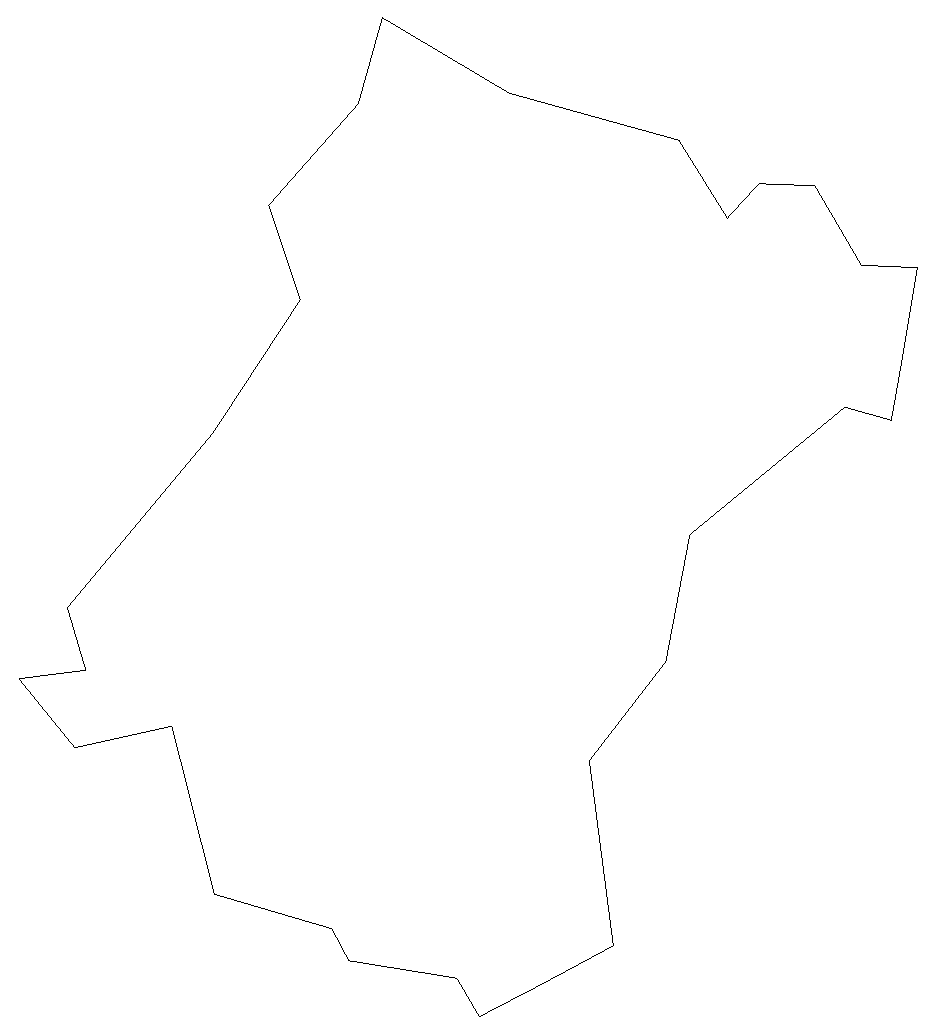
\includegraphics [scale=0.3]{grafiken/westpart.eps}
{\em\caption{\label{partgermany} Corresponding graph of the
section of the boundary file}}
\end{figure}

In some cases it might happen that a region is separated into
subregions that are not connected. As an illustrative example
compare \autoref{westsub} showing a region of Germany that is
separated into 8 subregions. In this case the {\em boundary file}
must contain the polygons of all subregions. The first row for
each of these subregions must contain the region code and the
number of lines the polygon of the respective subregion consists
of. Note that it is not necessary that the polygons of the
subregions are stored in subsequent order in the {\em boundary
file}.

Another special case that might occur is illustrated in
\autoref{westin}. Here a region is completely surrounded by
another region. In this case an additional line must be added to
the boundary description of the {\em surrounded} region. The
additional line must be placed  after the first line and must
contain the
region code of the {\em surrounding} region. The syntax is:

#is.in#,"{\em region code}"

The following lines show a section of the {\em boundary file} of
Germany, where region "9361" is totally
surrounded by region "9371":

\footnotesize

\hspace{1cm} $\vdots$

"9361",7 \\
is.in,"9371" \\
4155.84668,2409.58496 \\
4161.69922,2449.38330 \\
4201.49756,2461.08862 \\
4224.90820,2478.64673 \\
4250.66016,2418.94922 \\
4193.30371,2387.34448 \\
4155.84668,2409.58496

\hspace{1cm} $\vdots$

\normalsize

\begin{figure}[hb]
\centering

\includegraphics [scale=0.3]{grafiken/reg1054.eps}
{\em\caption{\label{westsub} Example for a region that is divided
into subregions}}
\end{figure}

\begin{figure}[hb]
\centering

\includegraphics [scale=0.3]{grafiken/westin.eps}
{\em\caption{\label{westin} Example for a region that is totally
surrounded by another region}}
\end{figure}



Finally, we want to draw attention to an important limitation in
the current version of {\em BayesX}. In most cases {\em map
objects} serve as auxiliary objects to estimate spatial effects
with {\em bayesreg objects} or {\em remlreg objects}. In this case the names of the regions
of the map and the values of the spatial covariate, whose effect
is estimated, must match. Since there are only numerical variables
allowed in {\em dataset objects} (and no string valued variables),
the names of the regions in the corresponding {\em map object}
must necessarily be numbers, although there is in principle no
limitation for the names of regions in {\em map objects}.

\subsubsection*{Structure of a graph file}

A graph file stores the nodes and the edges of a graph $G =
(N,E)$, see for example George and Liu (1981, Ch. 3) for a first
introduction into graph theory. A graph is a convenient way of
representing the neighborhood structure of a geographical map. The
nodes of the graph correspond to the region codes. The
neighborhood structure is represented by the edges of the graph.
In some situations it may be useful to define weights associated
with the edges of a graph which can be stored in the {\em graph
file} as well.

We now describe the structure of a {\em graph file} as it is expected by
{\em BayesX}. The first line of a {\em graph file} must contain
the total number of nodes of the graph. In the remaining lines,
the nodes of the graph together with their edges and associated
weights are specified. One node corresponds to three consecutive
lines. The first of the three lines must contain the name of the
node, which may simply be the name of a geographical region. In
the second line the number of edges of that particular node is
given. The third line contains the corresponding edges of the
node, where an edge is given by the index of a neighboring node.
The index starts with zero. For example, if the fourth and the
seventh node/region in the {\em graph file} are
connected/neighbors, the edge index for the fourth node/region is
6 and for the seventh node/region 3.

We illustrate the structure of a {\em graph file} with an example. The
following few lines are the beginning
of the {\em graph file} corresponding to the map of (former) West Germany:

\footnotesize

327 \\
9162 \\
3 \\
1 2 3 \\
9174 \\
6 \\
0 4 2 3 5 6 \\
9179 \\
6 \\
0 1 7 3 8 6

\hspace{1cm} $\vdots$

\normalsize

\vspace{0.5cm}

The first line specifies the total number of nodes, in the present
example 327 nodes. The subsequent three lines correspond to the
node with name '9162', which is the first region in the map of
West Germany. Region '9162' has 3 neighbors, namely the second,
third and fourth node appearing in the graph file. Once again,
note that the index starts with zero, i.e. 0 corresponds to the
first node, 1 corresponds to the second node and so on. Lines 5 to
7 in the example correspond to node '9174' and its neighbors and
lines 8 to 10 correspond to node '9179'.

In a {\em graph file} it is also possible to specify weights associated
with the edges of the nodes. Since in the preceding example no
weights are explicitly specified, all weights are automatically
defined to be equal to one. Nonequal weights are specified in the
{\em graph file} by simply adding them following the edges of a
particular node.
An example of the beginning of a {\em graph file} with weights is given below:

\footnotesize

327 \\
9162 \\
3 \\
1 2 3 0.4 1.2 0.7\\
9174 \\
6 \\
0 4 2 3 5 6 0.4 0.3 0.8 0.8 1.4 1.6\\
9179 \\
6 \\
0 1 7 3 8 6 1.2 0.8 0.2 1.8 1.7 1.3

\hspace{1cm} $\vdots$

\normalsize

\vspace{0.5cm}

Here the edges of the first node '9162' have weights 0.4, 1.2 and
0.7.\bigskip



\subheader{Options}

\begin{itemize}
\item #graph# \\
If #graph# is specified as an additional option, {\em BayesX}
expects a {\em graph file} to be read in rather than a {\em
boundary file}.
\item #weightdef=adjacency# $|$ #centroid#  $|$ #combnd# \\
\label{weightsmap} Option #weightdef# allows to specify how the
weights associated with each pair of neighbors are computed.
Currently there are three weight specifications available,
#weightdef=adjacency#, #weightdef=centroid# and
#weightdef=combnd#. If #weightdef=adjacency# is specified, for
each pair of neighbors the weights are set equal to one. The so
called adjacency weights are the most common ones in spatial
statistics. Specifying #weightdef=centroid# results in weights
proportional to the distance of the centroids of neighboring
regions. More specifically, the weight $w_{us}$ of two neighboring
regions $u$ and $s$ is set to $w_{us} = c \cdot \exp(-d(u,s))$,
where $d$ is the Euclidian distance between the centroids of the
two sites and $c$ is a normalizing constant. The constant $c$ is
chosen in such a way that the total sum of weights is equal to the
total number of neighbors, which is in analogy to adjacency
weights. The third choice #weightdef=combnd# results in weights
proportional to the length of the common boundary. Similarly to
#weightdef=centroid#, the weights are normalized, i.e. the total
sum of weights is equal to the number of neighbors.

Note that the specification of the #weightdef# option is only
meaningful if a {\em boundary file} is read. If a {\em graph file}
is read  instead, the option has no effect because the boundary
information of regions is missing and  the computation of weights
is therefore impossible.
\end{itemize}



\clearpage



\section{Method outfile}
\label{mapoutfile} \index{map object!outfile command}

\begin{stanza}{Description}

{Method #outfile# performs the reverse of the #infile# command.
Using method #outfile#, the map information currently in memory is
written to an external file. The map information can be written
either in {\em boundary file} or in {\em graph file} format.}
\end{stanza}

\begin{stanza}{Syntax}

{#># {\em objectname}.#outfile# [{\em , options}] #using# {\em
filename}

#outfile# writes the map information to the external file
specified in {\em filename}. The file format can be either a {\em
boundary file} or a {\em graph file}. If #graph# is specified as
an additional option, the file format will be a {\em graph file},
otherwise a {\em boundary file}.}
\end{stanza}

\subheader{Options}

\begin{itemize}
\item #graph# \\
Forces the program to store the map information in {\em graph
file} format rather than {\em boundary file} format.
\item #includeweights# \\
Option #includeweights# is meaningful only if the storing format
is a {\em graph file}, i.e. option #graph# is additionally
specified. In that case the weights associated with the edges
(neighbors) of the nodes (regions) are additionally stored.
\item #replace# \\
The #replace# option allows {\em BayesX} to overwrite an already
existing file. If #replace# is omitted in the optionlist and the
file specified in {\em filename} already exists, an error will be
raised. This prevents you from overwriting an existing file
unintentionally.
\end{itemize}



\clearpage



\section{Method reorder}
\label{mapreorder} \index{reorder regions of a map} \index{map
object!reorder command}

\begin{stanza}{Description}

{Method #reorder# reorders the regions of a map in the sense that
the adjacency matrix of the reordered map has the smallest
envelope when compared to all other possible orderings. A new map
should always be reordered before using it with {\em bayesreg
objects} because MCMC updates for spatial covariates will be much
faster if the envelope of the posterior precision matrix is small.
For reordering of the regions of the map the reverse Cuthill
Mc-Kee algorithm is used, see George and Liu (1981) p. 58 ff.}
\end{stanza}

\begin{stanza}{Syntax}

{#># {\em objectname}.#reorder#

#reorder# reorders the regions of a map in order to obtain
smallest envelope of the corresponding adjacency matrix.}
\end{stanza}

\begin{stanza}{Options}

{Not allowed.}
\end{stanza}

\begin{stanza}{Reference}

{\begin{description}

\item[George, A., Liu, J. W. (1981).] {\em Computer Solution of Large
Sparse Positive Definite Systems.} Series in computational
mathematics, Prentice--Hall.

\end{description}}
\end{stanza}


\chapter{graph objects}
\label{graphobj} \index{Graph object} \index{Visualizing data}

{\em Graph objects} are used to visualize data or estimation results obtained with the regression objects in the GUI
version of {\em BayesX}. No graph objects are available in the command line version of {\it BayesX}. However, the R package
accompanying {\it BayesX} provides similar functionality for visualising data and estimation results as implemented for {\it
graph objects}.

Currently, {\em graph objects} can be used to draw scatterplots between variables (\autoref{graphplot}, method #plot#), or to
draw and color geographical maps stored in {\em map objects} (\autoref{graphdrawmap}, method #drawmap#). The resulting plots
are either printed on the screen or stored as postscript files for further use in other documents (e.g. \LaTeX\/ documents).

A {\em graph object} is created by typing

#> graph# {\em objectname}

in the {\em command window}.


\clearpage


\section{Method drawmap}
\label{graphdrawmap} \index{Graph object!Drawmap command}
\index{Drawing geographical maps}

\begin{stanza}{Description}

Method #drawmap# is used to draw geographical maps and color the
regions according to some numerical characteristics.
\end{stanza}

\begin{stanza}{Syntax}

 #> #{\em objectname}.#drawmap#  [{\em plotvar regionvar}] [#if# {\em expression}], {\em #map#=mapname} [{\em options}]\\
 #> #[#using# {\em dataset}]

Method #drawmap# draws the map stored in the {\em map object} {\em
mapname} and prints the graph either on the screen or stores it as
a postscript file (if option #outfile# is specified). The regions
with regioncode {\em regionvar} are colored according to the
values of the variable {\em plotvar}. The variables {\em plotvar}
and {\em regionvar} are supposed to be stored in the {\em dataset
object} {\em dataset}. An #if# statement may be specified to use
only a part of the data in {\em dataset}. Several options are
available, e.g. for changing from grey scale to color scale or to
store the map as a postscript file. See the options list below for
more details.
\end{stanza}

\begin{stanza}{Options}

The most important option, which therefore is obligatory, is the
#map# option. This option specified the name of the {\em map
object} containing the boundary information to be drawn.
Additional options for method #drawmap# (in alphabetical order)
are:
\end{stanza}

\begin{itemize}
\item #color#

The #color# option allows to choose between a grey scale and a
colored scale. If the keyword #color# is specified, a colored
scale is used instead of a grey scale.

\item #drawnames#

In some situations it may be useful to print the names of the
regions into the graph (although the result will probably be
confusing in most cases). This can be achieved by specifying the
additional option #drawnames#. By default the names of the regions
are omitted in the map.

\item #fontsize = #{\em integer}

Specifies the font size (in pixels) for labelling the legend and
writing the names of the regions (if specified). Note, that the
title is scaled accordingly (see option #titlesize#). The default is
#fontsize=12#.

\item #hcl#

Requests that a color palette from the HCL color space should be
used instead of an RGB palette. The HCL colors will be selected
diverging from a neutral center (grey) to two different extreme
colors (red and green) in contrast to the RGB colors diverging
from yellow to red and green. HCL colors are particularly useful
for electronic presentations since they are device-independent.
The option #hcl# is only meaningful in combination with the option
#color#.

\item #lowerlimit = #{\em realvalue}

Lower limit of the range to be drawn. If #lowerlimit# is omitted,
the minimum numerical value in {\em plotvar} will be used as the
lower limit instead.

\item #map = #{\em mapname}

{\em mapname} specifies the name of the {\em map object}
containing the boundary information to be drawn. This option is
obligatory.

\item #nolegend#

By default a legend is drawn into the graph. Specifying the option
#nolegend# will exclude the legend from the graph.

\item #nrcolors = #{\em integer}

To color the regions according to their numerical characteristics,
the data are divided into a (typically large) number of ordered
categories. Afterwards a color is associated with each category.
The #nrcolors# option can be used to specify the number of
categories (and therefore the number of different colors). The
maximum number of colors is 256, which is also the default value.

\item #outfile = #{\em filename}

If option #outfile# is specified the graph will be stored as a
postscript file rather than being printed on the screen. The full
path and the filename have to be specified in {\em filename}. By
default, an error will be raised if the specified file is already
existing or if the path is invalid. To overwrite  an already
existing file, option #replace# has to be specified in addition.
This prevents you from overwriting your files unintentionally.

\item #pcat#

If you want to visualize posterior probabilities, it is convenient
to specify #pcat#. In this case, method #drawmap# expects a
variable containing only the values -1, 0 and 1. Of course you can
achieve the same result by setting #nrcolors=3#, #lowerlimit=-1#
and #upperlimit=1#.

\item #replace#

The #replace# option is only meanigful in combination with option
#outfile#. Specifying #replace# as an additional option allows the
program to overwrite an already existing file (specified in
#outfile#), otherwise an error will be raised.

\item #swapcolors#

In some situations it may be favorable to swap the order of the
colors, i.e. black (red) shades corresponding to large values and
white (green) shades corresponding to small values. This is
achieved by specifying #swapcolors#. By default, small values are
colored in black shades (red shades) and large values in white
shades (green shades).

\item #title = #{\em characterstring}

Adds a title to the graph. If the title contains more than one
word, {\em characterstring} must be enclosed by quotation marks
(e.g. #title="my first map"#).

\item #titlesize = #{\em realvalue}

Specifies the factor by which the size of the title is scaled
relative to the size of the labels of the legend (compare option
#fontsize#). The default is #titlesize=1.5#.

\item #upperlimit = #{\em realvalue}

Upper limit of the range to be drawn. If #upperlimit# is omitted,
the maximum numerical value in {\em plotvar} will be used as the
upper limit instead.

\end{itemize}

\begin{stanza}{Example}

This example shows how to draw the map of Munich and how to color
the subquarters in Munich according to some numerical
characteristics. The boundary file of Munich (#munich.bnd#) as
well as the data set #rent94means.raw# containing the distribution
of the average rents across subquarters are included in the
subfolder #examples# of the {\em BayesX} installation directory.
In the following we assume that {\em BayesX} is installed in the
folder #c:\bayesx#. We start by creating a {\em dataset object}
#d# and a {\em map object} #m# and proceed with reading the rent
data set and the map of Munich:

#> dataset d# \\
#> d.infile using c:\bayesx\examples\rent94means.raw#

#> map m# \\
#> m.infile using c:\bayesx\examples\munich.bnd#

Afterwards we create a {\em graph object} #g# and draw the map of
Munich:

#> graph g# \\
#> g.drawmap , map=m#

\begin{figure}[htb]
\begin{center}
\includegraphics[scale=0.5]{grafiken/munichdrawmap.ps}
{\em\caption{ \label{munichdrawmap} Map of Munich}}
\end{center}
\end{figure}

The map of Munich appears on the screen in a separate window,
compare \autoref{munichdrawmap}. Before closing the window you are
asked whether you want to save the map or not. If you agree the
map will be stored as a postscript file in the folder you specify.
Of course, the map can be directly stored in postscript format
using the #outfile# option. In this case the map is not shown on
the screen. Typing

#> g.drawmap , map=m outfile=c:\temp\munich.ps#

stores the map of Munich in the file #c:\temp\munich.ps# and the
graph is not printed on the screen.

Usually maps are drawn to visualize numerical characteristics of
their regions. For instance, typing

#> g.drawmap R L , map=m color using d#

displays the distribution of the average rents #R# across
subquarters #L#, see \autoref{munichmeans}. The areas in the
figure shaded with diagonal lines mark subquarters for which  no
data are available. The specification of the second variable #L#
is required to match the names of the subquarters stored in the
{\em map object} #m# with the data set #d#. Option #color# is
specified to obtain a colored graph. Specifying option #hcl# in
addition yields the same information visualized in HCL colors (see
\autoref{munichmeanshcl}).

#> g.drawmap R L , map=m color hcl using d#

\end{stanza}

\begin{figure}[htb]
\begin{center}
\includegraphics[scale=0.5]{grafiken/munichmeansdrawmap.ps}
{\em\caption{ \label{munichmeans} Distribution of the average rents
per square meter in Munich visualized in RGB colors.}}
\end{center}
\end{figure}

\begin{figure}[htb]
\begin{center}
\includegraphics[scale=0.5]{grafiken/munichmeansdrawmaphcl.ps}
{\em\caption{ \label{munichmeanshcl} Distribution of the average
rents per square meter in Munich visualized in HCL colors.}}
\end{center}
\end{figure}

\clearpage

\section{Method plot}
\label{graphplot} \index{Graph object!Plot command}
\index{Scatterplot} \index{Drawing scatterplots}

\begin{stanza}{Description}

{Method #plot# is used to draw scatterplots between two or more
variables. Several options for labelling axes, connecting points,
saving the graph etc. are available.}
\end{stanza}

\begin{stanza}{Syntax}

{#> #{\em objectname}.#plot#  {\em xvar yvar1} [{\em yvar2 yvar3}
\dots]
[#if# {\em expression}] [, {\em options}] #using# {\em dataset}

Method #plot# draws scatterplots of {\em yvar1}, {\em yvar2}, {\em
yvar3} $\dots$ against {\em xvar} into a single graph using the
data set specified in {\em dataset}. An #if# statement may be used
to apply the method only to a part of the data. In addition,
several options may be specified for labelling axes, connecting
points, saving the graph in postscript format etc., see the
options list below.}
\end{stanza}

\begin{stanza}{Options}

{The following options are available for method #plot# (listed in
alphabetical order):}
\end{stanza}

\begin{itemize}
\item #connect = 1#$|$#2#$|$#3#$|$#4#$|$#5#[{\em specifications
for further variables}]

Option #connect# specifies how points in the scatterplot are
connected. There are currently 5 different specifications:

\begin{tabular}{ll}
#1# & draw straight lines between the points (default) \\
#2#, #3#, #4# & draw dashed lines (numbers 2 -- 4 indicate different variants)\\
#5# & do not connect, i.e.~plot points only \\
\end{tabular}

If you draw more than one scatterplot in the same graph (i.e. more
than one {\em yvar} is specified) the points for each {\em yvar}
can be connected differently by specifying the corresponding
number (#1,2,3,4,5#) separately for every {\em yvar}. Typing for
example

#connect=15#

connects the points corresponding to {\em yvar1} and {\em xvar} by
straight lines, but does not connect the points corresponding to
{\em yvar2} (if specified) and {\em xvar}. Points corresponding to
additional variables $yvar3$, etc.~are connected by straight lines
(the default).

An equivalent way of specifying the different variants is
available via the symbols '#l#', '#d#', '#_#', '#-#' and '#p#',
which correspond to the numbers 1-5, i.e.~

#connect=12345# is equivalent to #connect=ld_-p#

\item #fontsize = #{\em integer}

Specifies the font size (in pixels) for labelling axes etc. Note
that the title is scaled accordingly. The default is
#fontsize=12#.

\item #height = #{\em integer}

Specifies the height (in pixels) of the graph. The default is
#height=210#.

 \item #linecolor = B#$|$#b#$|$#c#$|$#G#$|$#g#$|$#o#$|$#m#$|$#r#$|$#y# [{\em specifications
for further variables}]

Option #linecolor# specifies the color to be used for drawing
lines (or points, see option #connect#) in the scatterplot.
Currently the following specifications are available:

\begin{tabular}{ll}
#B# & black (default) \\
#b# & blue \\
#c# & cyan \\
#G# & gray \\
#g# & green \\
#o# & orange \\
#m# & magenta \\
#r# & red \\
#y# & yellow \\
\end{tabular}

If you draw more than one scatterplot in the same graph (i.e. more
than one {\em yvar} is specified) you can use different colors for
each {\em yvar} by simply specifying the corresponding symbol
(#B,b,c,G,g,o,m,r,y#) for each {\em yvar}. Typing for example

#linecolor = Bgr#

colors the lines (points) corresponding to {\em yvar1} and {\em
xvar} in black, whereas the points corresponding to {\em yvar2}
and {\em yvar3} (if specified) and {\em xvar} are colored in green
and red, respectively.

\item #linewidth = #{\em integer}

Specifies how thick lines should be drawn. The default is
#linewidth=5#.

\item #outfile = #{\em filename}

If option #outfile# is specified, the graph will be stored as a
postscript file rather than being printed on the screen. The full
path and the filename have to be specified in {\em filename}. By
default, an error will be raised if the specified file is already
existing or if the specified folder is not valid. To overwrite an
already existing file, option #replace# must be specified in
addition. This prevents you from overwriting your files
unintentionally.

\item #pointsize = #{\em integer}

Specifies the size of the points (in pixels) if drawing points
rather than lines. The default is #pointsize=20#.

\item #replace#

The #replace# option is useful only in combination with option
#outfile#. Specifying #replace# as an additional option allows the
program to overwrite an already existing file (specified in
#outfile#), otherwise an error will be raised.

\item #title = #{\em characterstring}

Adds a title to the graph. If the title contains more than one
word, {\em characterstring} must be enclosed by quotation marks (e.g.
#title="my first title"#).

\item #titlesize = #{\em realvalue}

Specifies the factor by which the size of the title is scaled
relative to the size of the labels of the axes (compare option
#fontsize#). The default is #titlesize=1.5#.

\item #width = #{\em integer}

Specifies the width (in pixels) of the graph. The default is
#width=356#.

\item #xlab = #{\em characterstring}

Labels the x-axis. If the label contains more than one word, {\em
characterstring} must be enclosed by quotation marks (e.g.
#xlab="x axis"#).

\item #xlimbottom = #{\em realvalue}

Specifies the minimum value at the x-axis to be drawn. The default
is the minimum value in the data set. If #xlimbottom# is above the
minimum value in the data set, only a part of the  graph will be
visible.

\item #xlimtop = #{\em realvalue}

Specifies the maximum value at the x-axis to be drawn. The default
is the maximum value in the data set. If #xlimtop# is below the
maximum value in the data set, only a part of the  graph will be
visible.

\item #xstart = #{\em realvalue}

Specifies the value where the first tick on the x-axis should be
drawn. The default is the minimum value on the x-axis.

\item #xstep = #{\em realvalue}

If #xstep# is specified, ticks are drawn at the x-axis with
stepwidth {\em realvalue} starting at the minimum value on the
x-axis (or at the value specified in option #xstart#). By default,
five equally spaced ticks are drawn at the x-axis.

\item #ylab = #{\em characterstring}

Labels the y-axis. If the label contains more than one word, {\em
characterstring} must be enclosed by quotation marks (e.g.
\texttt{ylab="y axis"}).

\item #ylimbottom = #{\em realvalue}

Specifies the minimum value at the y-axis to be drawn. The default
is the minimum value in the data set. If #ylimbottom# is above the
minimum value in the data set, only a part of the  graph will be
visible.

\item #ylimtop = #{\em realvalue}

Specifies the maximum value at the y-axis to be drawn. The default
is the maximum value in the data set. If #ylimtop# is below the
maximum value in the data set, only a part of the  graph will be
visible.

\item #ystart = #{\em realvalue}

Specifies the value where the first tick on the y-axis should be
drawn. The default is the minimum value on the y-axis.

\item #ystep = #{\em realvalue}

If #ystep# is specified,  ticks are drawn at the y-axis with
stepwidth {\em realvalue} starting at the minimum value on the
y-axis (or at the value specified in option #ystart#). By default,
five equally spaced ticks are drawn at the y-axis.

\item Further options for representing dates

In the following we describe options that may be useful if the
variable on the x-axis represents dates. An example is a variable
with values ranging from 1 to 19, representing the time period
from January 1983 to July 1984. In this case, we might prefer that
the x-axis is labelled in terms of dates rather than in the
original coding (from 1 to 19). To achieve this, {\em BayesX}
provides the options #month#, #year# and #xstep#. Options #year#
and #month# are used to specify the year and the month (1 for
January, 2 for February, \dots) corresponding to the minimum
covariate value. In the example mentioned above #year=1983# and
#month=1# will produce the correct result. In addition, option
#xstep# may be specified to define the periodicity in which your
data are collected. For example #xstep=12# (the default)
corresponds to monthly data, while #xstep = 4#, #xstep = 2# and
#xstep = 1# correspond to quarterly, half yearly and yearly data,
respectively.
\end{itemize}


\begin{stanza}{Example}

{We use the Munich rent data set #rent94.raw# to demonstrate the
usage of method #plot#. The data set is included in the subfolder
#examples# of the {\em BayesX} installation directory. In the
following we assume that {\em BayesX} has been installed to the
folder #c:\bayesx#. We start by reading the data by typing:

#> dataset d# \\
#> d.infile using c:\bayesx\examples\rent94.raw#

Then we generate a {\em graph object} #g# and draw a scatterplot
between floor space (variable #F#) and rent per square meter
(variable #R#):

#> graph g# \\
#> g.plot R F using d#

The strange picture shown in \autoref{plotrf1} appears on the
screen. The problem is that the points are connected by straight
lines although the values of #F# are not sorted. Hence, to obtain
an improved scatterplot, we could either sort the data set with
respect to #F# or simply avoid connecting the points. Typing

#> d.sort F# \\
#> g.plot R F using d#

yields the first option. Typing

#> g.plot R F, connect=p using d#

yields the second option mentioned above. The corresponding graphs
are shown in \autoref{plotrf2} and \autoref{plotrf3},
respectively. To further improve the appearance of the scatterplot
we add a title and label the x- and y-axes
by typing

#> g.plot R F, title="scatterplot between F and R" ylab="rent"# \\
#  xlab="floor space in square meters" connect=p using d#

The result is shown in \autoref{plotrf4}.
Finally, we add the outfile option to save the graph in postscript format:

 #> g.plot R F, title="scatterplot between F and R" ylab="rent" #\\
 #  xlab="floor space in square meters" connect=p#\\
 #  outfile=c:\temp\plotrf.ps using d #

\begin{figure}[ht]
\begin{center}
\includegraphics[scale=0.7]{grafiken/plotrf1.ps}
{\em\caption{ \label{plotrf1} Scatterplot between floor space and
rent per square meters (first try).}}
\end{center}
\end{figure}

\begin{figure}[ht]
\begin{center}
\includegraphics[scale=0.7]{grafiken/plotrf2.ps}
{\em\caption{ \label{plotrf2} Scatterplot between floor space and
rent per square meters (second try).}}
\end{center}
\end{figure}

\begin{figure}[ht]
\begin{center}
\includegraphics[scale=0.7]{grafiken/plotrf3.ps}
{\em\caption{ \label{plotrf3} Scatterplot between floor space and
rent per square meters (third try).}}
\end{center}
\end{figure}

\begin{figure}[ht]
\begin{center}
\includegraphics[scale=0.7]{grafiken/plotrf4.ps}
{\em\caption{ \label{plotrf4} Scatterplot between floor space and
rent per square meters (final try).}}
\end{center}
\end{figure}
}
\end{stanza}
\clearpage



\clearpage



\section{Method plotautocor}
\label{graphplotautocor} \index{Graph object!Plotautocor command}
\index{Plotting autocorrelations}

\begin{stanza}{Description}

{Method #plotautocor# visualizes the autocorrelation functions
obtained with method #autocor# of {\em bayesreg objects}, see also
\autoref{bayesautocorr}.}
\end{stanza}


\begin{stanza}{Syntax}

{#> #{\em objectname}.#plotautocor# [,{\em options}] #using# {\em dataset}

Plots the autocorrelation functions stored in {\em dataset}. The
data set must have the special structure described in
\autoref{bayesautocorr}, i.e. method #plotautocor# is meaningful
only if Bayesian regression models have been estimated in advance
using {\em bayesreg objects} and autocorrelation functions of
sampled parameters have been computed using method #autocor# of
{\em bayesreg objects}.}
\end{stanza}

\subheader{Options}

\begin{itemize}
\item #mean#

If option #mean# is specified, only minimum, mean and maximum
autocorrelations are plotted for each lag number and model term.
This typically leads to a considerable reduction in computing time
and storing size.

\item #outfile = #{\em filename}

If option #outfile# is specified, the graph will be stored as a
postscript file instead of being printed on the screen. The path
and the filename have to be specified in {\em filename}. An error
will be raised if the specified file is already existing and the
#replace# option has not been specified.

\item #replace#

The #replace# option is only meaningful in combination with option
#outfile#. Specifying #replace# as an additional option allows the
program to overwrite an already existing file (specified in
#outfile#), otherwise an error will be raised.
\end{itemize}



\clearpage



\section{Method plotsample}
\label{graphplotsample} \index{Graph object!Plotsample command}
\index{Plotting sampled parameters} \index{Sampling paths}

\begin{stanza}{Description}

{Method #plotsample# visualizes the sampling paths of sampled
parameters obtained with method #getsample# of {\em bayesreg
objects}, see also \autoref{bayesgetsample}. The application of
method #plotsample# is meaningful only if Bayesian regression
models have been estimated in advance using {\em bayesreg objects}
and sampled parameters have been computed and stored using method
#getsample#.}
\end{stanza}

\begin{stanza}{Syntax}

{#> #{\em objectname}.#plotsample# [,{\em options}] #using# {\em dataset}

Plots sampled parameters stored in {\em dataset}. The data set
must have the special structure described in
\autoref{bayesgetsample}.}
\end{stanza}

\subheader{Options}

\begin{itemize}
\item #outfile = #{\em filename}

If option #outfile# is specified, the graph will be stored as a
postscript file instead of being printed on the screen. The full
path and the filename have to be specified in {\em filename}. An
error will be raised if the specified file is already existing and
the #replace# option has not been specified.

\item #replace#

The #replace# option is only useful in combination with option
#outfile#. Specifying #replace# as an additional option allows the
program to overwrite an already existing file (specified in
#outfile#), otherwise an error will be raised.
\end{itemize}


\chapter{bayesreg objects}
\label{bayesreg} \index{Bayesreg object}

{\em bayesreg objects} are used to fit (multivariate) exponential family, hazard rate or multi-state models with {\em
structured additive predictor} subsumed in the class of {\em structured additive regression (STAR)} models, see \citeasnoun{FahKneLan04}.
Inference is based on fully Bayesian approach implemented via Markov Chain Monte Carlo (MCMC)
simulation techniques. The methodology manual provides brief introduction to structured additive regression and MCMC-based
inference. More details can be found in \citeasnoun{FahLan01a}, \citeasnoun{FahLan01b}, \citeasnoun{LanBre04},
\citeasnoun{BreLan06}, \citeasnoun{FahOsu03} and \citeasnoun{HenBreFah06}. Good introductions to
generalized linear models are the monographs of \citeasnoun{FahTut01} and \citeasnoun{McCNel89}. Introductions to semi- and
nonparametric models are given in \citeasnoun{GreSil94}, \citeasnoun{HasTib90}, \citeasnoun{HasTibFri01} or \citeasnoun{Woo06a}.
The paper of \citeasnoun{ChiGre95}, the monograph {\em Markov Chain Monte Carlo in Practice} edited by
\citeasnoun{GilRicSpi96} and the introductory article by \citeasnoun{Gre01} give a thorough overview over MCMC simulation
techniques.

First steps with {\em bayesreg objects} can be done with the
tutorial like example in chapter \ref*{zambiaanalysis} of the
tutorials manual which provides a self-contained demonstrating
example.

\clearpage

\section{Method regress}
\label{bayesregress} \index{Bayesreg object!Regress
function}\index{Regress function}

\subsection{Description}
\label{bayesregregressdescr}

Method #regress# estimates a structured additive regression model.

\index{Generalized linear models} \index{Generalized additive
models} \index{Varying coefficients} \index{Bayesian semiparametric
regression} \index{MCMC} \index{Markov chain Monte Carlo}

\subsection{Syntax}\index{Regression syntax}\index{Bayesreg object!Regression syntax}
\label{bayesregregresssyntax}

 #> #{\em objectname}.#regress# {\em model} [#weight# {\em weightvar}] [#if# {\em expression}] [{\em , options}] #using# {\em dataset}

Method #regress# estimates the regression model specified in {\em
model} using the data specified in {\em dataset}. {\em dataset}
has to be the name of a {\em dataset object} created before. The
details of correct models are covered in \autoref{modelsyntax}.
The distribution of the response variable can be either Gaussian,
gamma, binomial, multinomial, Poisson, negative binomial, zero
inflated Poisson or zero inflated negative binomial. In addition,
{\em BayesX} supports continuous time survival and multi-state
models, see also \autoref{familyopt} for a more detailled
overview. The response distribution is specified using option
#family#, see \autoref{familysyntax} below and the options list in
\autoref{regressoptions}. The default value is #family=binomial#
with a logit link. An #if# statement may be specified to analyze
only parts of the data set, i.e.~the observations where {\em
expression} is true.

\subsubsection{Optional weight variable}\index{Weighted regression}
\label{weightspecification}

An optional weight variable {\em weightvar} may be specified to
estimate weighted regression models. For Gaussian responses {\em
BayesX} assumes that $y_r|\eta_r,\sigma^2 \sim
N(\eta,\sigma^2/weightvar_r)$. Thus, for grouped Gaussian
responses the weights must be the number of observations in the
groups if the $y_r$'s are the average of individual responses. If
the $y_r$'s are the sum of responses in every group, the weights
have to be the reciprocal of the number of observations in the
groups. Of course, estimation of usual weighted regression models
with heteroscedastic errors is also possible. In this case the
weights should be proportional to the reciprocal of the
heteroscedastic variances. If the response distribution is
binomial, it is assumed that the values of the weight variable
correspond to the number of replications and that the values of
the response variable itself correspond to the number of
successes. If #weight# is omitted, {\em BayesX} assumes that the
number of replications is one, i.e.~the values of the response
must be either zero or one. For grouped Poisson data the weights
have to be the number of observations in a group and the $y_i$'s
are assumed to be the average of individual responses. In the case
of gamma distributed responses, {\em BayesX} assumes $y_r \sim
G(\exp(\eta_r),\nu/weightvar_r)$ where $\mu_r= \exp(\eta_r)$ is
the mean and $s_r = \nu/weightvar_r$ is the scale parameter.

If estimation is based on latent utility representations, the
specification of weights is not allowed. Similarly, for negative
binomial, zero inflated Poisson and zero inflated negative
binomial models as well as hazard regression and multi-state
models, weighted regression is not implemented yet.

\subsubsection{Syntax of possible model terms}
\label{modelsyntax}\index{Model terms}\index{Bayesreg object!Model
terms}

The general syntax of models is:

$depvar = term_1 + term_2 + \cdots + term_r$

where {\em depvar} specifies the dependent variable in the model
and $term_1$,\dots,$term_r$ define the specific form of covariate
effects on the dependent variable. The different terms have to be
separated by '+' signs. A constant intercept is automatically
included in the models and does not have to be requested by the
user. This section reviews all possible model terms that are
currently supported by {\em bayesreg objects} and provides some
specific examples. Note that all described terms may be combined
in arbitrary order. An overview about the capabilities of {\em
bayesreg objects} is given in \autoref{terms}.
\autoref{bayesreginteractions} shows how interactions between
covariates are specified. Full details about all available options
are given in \autoref{localoptions}.

Throughout this section #Y# will denote the dependent variable.

\subsubsection*{Offset}\index{Offset}

\begin{itemize}
\item[] {\em Description}: Adds an offset term to the predictor.
\item[] {\em Predictor}: $\eta =  \cdots + \mbox{\it offs} + \cdots$
\item[] {\em Syntax}: #offs(offset)#
\item[] {\em Example}:

The following model statement can be used to estimate a Poisson
model with #offs# as offset term and #W1# and #W2# as fixed
effects (if #family=poisson# is specified in addition):

#Y = offs(offset) + W1 + W2#

\end{itemize}

\subsubsection*{Fixed effects}\index{Fixed effects}

\begin{itemize}
\item[] {\em Description}: Incorporates covariate #W1# as a fixed effect into the model.
\item[] {\em Predictor}: $\eta =  \cdots + \gamma_1 W1 + \cdots$
\item[] {\em Syntax}: #W1#
\item[] {\em Example}:

The following model statement specified a model with $q$ fixed
(linear) effects:

\texttt{Y = W1 + W2 + $\cdots$ + Wq}
\end{itemize}

\subsubsection*{Nonlinear effects of continuous covariates and time
scales}\index{Nonlinear effects}\index{Random
walks}\index{P-splines}


\begin{itemize}
 \item[]{\bf\sffamily First or second order random walk}
 \item[]{\em Description}: Defines a first or second order random walk
 prior for the effect of #X1#.
 \item[]{\em Predictor}: $\eta = \cdots + f_1(X1) + \cdots $
 \item[] {\em Syntax}:

#X1(rw1#[, {\em options}]#) #

#X1(rw2#[, {\em options}]#) #
\item[] {\em Example}:

Suppose that #X1# is a continuous covariate with possibly
nonlinear effect. The following model statement defines a second
order random walk prior for $f_1$:

#Y = X1(rw2,a=0.001,b=0.001)#

The term #X1(rw2,a=0.001,b=0.001)# indicates, that the effect of
#X1# should be included nonparametrically using a second order
random walk prior. A first order random walk is obtained by
modifying the first argument in #X1(rw2,a=0.001,b=0.001)# from
#rw2# to #rw1# yielding #X1(rw1,a=0.001,b=0.001)#. The second and
third argument in the expression above are used to specify the
hyperparameters of the inverse gamma prior for the variance of the
random walk. Besides the options #a# and #b#, some more options
are available, see \autoref{localoptions} for details.

\item[] {\bf\sffamily P-spline with first or second order random
walk penalty}

\item[] {\em Description}: Defines a P-spline with a first or
second order random walk penalty for the parameters of the spline.
\item[] {\em Predictor}: $\eta =  \cdots + f_1(X1) + \cdots$
\item[] {\em Syntax}:

#X1(psplinerw1#[{\em , options}]#) #

#X1(psplinerw2#[{\em , options}]#) #
\item[] {\em Example}:

A P-spline with second order random walk penalty is obtained by:

#Y = X1(psplinerw2)#

By default, the degree of the spline is 3 and the number of inner
knots is 20. The following model term defines a quadratic P-spline
with 30 knots:

#Y = X1(psplinerw2,degree=2,nrknots=30)#

Full details about all possible options for P-splines are given in
\autoref{localoptions}.

\item[] {\bf\sffamily Seasonal effect of a time scale}

\item[] {\em Description}: Defines a seasonal effect of #time#.
\item[] {\em Predictor}: $\eta =  \cdots + f_{season}(time) +
\cdots $ \item[] {\em Syntax}:

#time(season#[, {\em options}]#) #
\item[] {\em Example}:

A seasonal component for a time scale #time# is specified by

#Y = time(season,period=12)#.

where the second argument specifies the period of the seasonal
effect. In the example above the period is 12, corresponding to
monthly data.
\end{itemize}


\subsubsection*{Spatial Covariates}\index{Spatial
effects}\index{Markov random fields}\index{Two-dimensional P-spline}

\begin{itemize}
\item[]{\bf\sffamily Markov random field}

\item[] {\em Description}:

Defines a Markov random field prior for the spatial covariate
#region#. {\em BayesX} allows to incorporate spatial covariates
with geographical information stored in the {\em map object}
specified in option #map#.

\item[] {\em Predictor}: $\eta = \cdots + f_{spat}(region) +
\cdots$

\item[] {\em Syntax}:

#region(spatial,map=#{\em characterstring}#[#{\em , options}]#) #
\item[] {\em Example}:

For the specification of a Markov random field prior, #map# is an
obligatory argument that represents the name of a {\em map object}
(see \autoref{map}) containing all necessary spatial information
about the geographical map, i.e.~the neighbors of each region and
the weights associated with the neighbors. For example the
statement

#Y = region(spatial,map=germany)#

defines a Markov random field prior for #region# where the
geographical information is stored in the {\em map object}
#germany#. An error will be raised if #germany# is not existing.
It is advisable to reorder the regions of a map prior to
estimation of a spatial effect to obtain a band matrix like
precision matrix. This can be achieved using method #reorder# of
{\em map objects}, see \autoref{mapreorder} for details.

\item[]{\bf\sffamily Two-dimensional P-spline with first order
random walk penalty}

\item[] {\em Description}:

Defines a two-dimensional P-spline for the spatial covariate
#region# with a two-dimensional first order random walk penalty
for the parameters of the spline. Estimation is based on the
coordinates of the centroids of the regions. The centroids are
computed using the geographical information stored in the {\em map
object} specified in the option #map#.

\item[] {\em Predictor}: $\eta= \cdots + f(centroids) + \cdots$

\item[] {\em Syntax}:

#region(geospline,map=#{\em characterstring}#[, #{\em options}]#) #
\item[] {\em Example}:

For the specification of a two-dimensional P-spline ({\em
geospline}) #map# is an obligatory argument indicating the name of
a {\em map object} (see \autoref{map}) that contains all necessary
spatial information about the geographical map, i.e.~the neighbors
of each region and the weights associated with the neighbors. The
model term

#Y = region(geospline,map=germany)#

specifies a two-dimensional cubic P-spline with first order random
walk penalty where the geographical information is stored in the
{\em map object} #germany#.
\end{itemize}

\subsubsection*{Unordered group indicators}\index{Unordered group
indicators}\index{Random effects}\index{Random intercept}

\begin{itemize}
\item[]{\bf\sffamily Unit- or cluster-specific unstructured
effect}

\item[] {\em Description}: Defines an unstructured (uncorrelated)
random effect with respect to grouping variable #grvar#. \item[]
{\em Predictor}: $\eta = \cdots + f(grvar) + \cdots$ \item[] {\em
Syntax}:

#grvar(random#[, {\em options}]#) #
\item[] {\em Example}:

Gaussian i.i.d.~random effects allow to cope with unobserved
heterogeneity among units or clusters of observations. Suppose the
analyzed data set contains a group indicator #grvar# that gives
information about the individual or cluster a particular
observation belongs to. Then an individual-specific uncorrelated
random effect is defined by

#Y = grvar(random)#

The inclusion of more than one random effect term in the model is
possible, leading to the estimation of multilevel models. However,
we have only limited experience with multilevel models so that it
is not clear how well these models can be estimated in {\em
BayesX}.
\end{itemize}

\subsubsection*{Nonlinear baseline effect in hazard regression or multi-state models}
\index{Baseline}\index{Cox model}\index{Multi-state model}

\begin{itemize}
\item[]{\bf\sffamily P-spline with second order random walk
penalty}

\item[] {\em Description}: Defines a P-spline with second order
random walk penalty for the parameters of the spline for the
log-baseline effect $\log(\lambda_0$(#time#)). \item[] {\em
Predictor}: $\eta = \log(\lambda_0(time)) + \cdots$ \item[] {\em
Syntax}:

#time(baseline#[, {\em options}]#) #
\item[] {\em Example}:

Suppose continuous-time survival data (#time#, #delta#) together
with additional covariates (#W1#,#X1#) are given where #time#
denotes the vector of observed duration times, #delta# is the
vector of corresponding indicators of non-censoring, #W1# is a
discrete covariate, and #X1# is a continuous covariate. The
following continuous time survival model with hazard rate
$\lambda$ and log-baseline effect $\log(\lambda_0$(#time#))
\[
\lambda(time)=\lambda_0(time)\exp (\gamma_0 + \gamma_1 W1 + f(X1)
)=\exp\left(\log(\lambda_0(time)) + \gamma_0 + \gamma_1 W1 +
f(X1)\right)
\]
is estimated by the model statement

#delta = time(baseline) + W1 + X1(psplinerw2)#

Similarly, baseline effects on the transition intensities can be
specified in multi-state models.
\end{itemize}

\subsubsection*{Varying coefficients with continuous covariates as
effect modifier}\index{Varying coefficients}

\begin{itemize}
\item[]{\bf\sffamily First or second order random walk}

\item[] {\em Description}:

Defines a varying coefficient term, where the effect of #X1#
varies smoothly over the range of #X2#. Therefore covariate #X2#
is called the effect modifier. The smoothness prior for $f(X2)$ is
a first or second order random walk. \item[] {\em Predictor}:
$\eta= \cdots + f(X2)X1 + \cdots$ \item[] {\em Syntax}:

#X1*X2(rw1#[, {\em options}]#) #

#X1*X2(rw2#[, {\em options}]#) #
\item[] {\em Example}:

A varying coefficient term with a second order random walk
smoothness prior is defined as follows:

#Y = X1*X2(rw2)#

\item[] {\bf\sffamily P-spline with first or second order random
walk penalty}

\item[] {\em Description}:

Defines a varying coefficient term, where the effect of #X1#
varies smoothly over the range of #X2#. The smoothness prior for
$f(X2)$ is a P-spline with first or second order random walk
penalty. \item[] {\em Predictor}: $\eta= \cdots + f(X2)X1 +
\cdots$ \item[] {\em Syntax}:

#X1*X2(psplinerw1#[, {\em options}]#) #

#X1*X2(psplinerw2#[, {\em options}]#) #
\item[] {\em Example}:

A varying coefficient term with a second order random walk
smoothness prior is defined as follows:

#Y = X1*X2(psplinerw2)#

\item[]{\bf\sffamily Seasonal prior}

\item[] {\em Description}:

Defines a varying coefficients term where the effect of #X1#
varies over the range of the effect modifier #time#. A seasonal
prior is assumed for the effect of #time#.

\item[] {\em Predictor}: $\eta= \cdots + f_{season}(time)X1 +
\cdots $

\item[] {\em Syntax}:

#X1*time(season#[, {\em options}]#) #
\item[] {\em Example}:

The inclusion of a varying coefficients term with a seasonal prior
may be meaningful if we expect a different seasonal effect with
respect to a binary variable #X1#. In this case we can include an
additional seasonal effects for observations with #X1#=1 by

#Y = X1*time(season) #

\end{itemize}

\subsubsection*{Time-varying effects in hazard regression or multi-state models}
\index{Time-varying effects}

\begin{itemize}
\item[]{\bf\sffamily P-spline with second order random walk
penalty}

\item[] {\em Description}: Defines a varying coefficients term
where the effect of #X1# varies over the range of the effect
modifier #time#, i.e. variable #X1# is assumed to have a
time-varying effect. The smoothness prior for $f($#time#$)$ is a
P-spline with second order random walk penalty.

 \item[] {\em Predictor}: $\eta = \log(\lambda_0(time)) +
f(time)X1 \cdots$ \item[] {\em Syntax}:

 #X1*time(baseline#[, {\em options}]#) #
 \item[] {\em Example}:

Suppose continuous-time survival data (#time#, #delta#) together
with an additional covariate #X1# are given, where #time# denotes
the vector of observed duration times and #delta# is the vector of
corresponding indicators of non-censoring. The following Cox model
with hazard rate
\begin{eqnarray*}
 \lambda(time) & = & \lambda_0(time)\exp(\gamma_0 + f(time)X1)\\
 & = & \exp\left(\log(\lambda_0(time)) + \gamma_0 + f(time)X1\right)
\end{eqnarray*}
is estimated by the model statement

#delta = time(baseline) + X1*time(baseline)#

Similarly, time-varying effects on the transition intensities can
be specified in multi-state models.
\end{itemize}


\subsubsection*{Varying coefficients with spatial covariates as
effect modifiers}

\begin{itemize}
\item[]{\bf\sffamily Markov random field}

\item[] {\em Description}:

Defines a varying coefficients term where the effect of #X1#
varies smoothly over the range of the spatial covariate #region#.
A Markov random field is estimated for $f_{spat}($#region#$)$. The
geographical information is assumed to be stored in the {\em map
object} specified in the option #map#.

\item[] {\em Predictor}: $\eta = \cdots + f_{spat}(region)X1 +
\cdots$

\item[] {\em Syntax}:

#X1*region(spatial,map=#{\em characterstring}#[,#{\em options}]#) #
\item[] {\em Example}:

The statement

#Y = X1*region(spatial,map=germany) #

defines a varying coefficient term with the spatial covariate
#region# as the effect modifier and a Markov random field as spatial
smoothness prior. Weighted Markov random fields can be estimated by
including an appropriate weight definition when creating the {\em
map object} #germany# (see \autoref{mapinfile}).
\end{itemize}


%{\em Two-dimensional P-spline with first order random walk penalty}
%\begin{itemize}
%\item[] {\em Description}:

%Defines a varying coefficients term where the effect of X1 varies
%smoothly over the range of the spatial covariate X2. A 2
%dimensional P-spline based on the tensor product of one-dimensional
%P-splines with a two-dimensional first order random walk penalty for
%the parameters of the spline is estimated for $f$. The centroids
%are computed using the geographical information stored in the map
%object specified through the option #map#.
%\item[] {\em Predictor}: $\eta= \cdots + f(centroids)X1 + \cdots$
%\item[] {\em Syntax}:

%X1*X2(geospline,map=characterstring[, options])
%\item[] {\em Example}:
%\end{itemize}


\subsubsection*{Varying coefficients with unordered group indicators as effect modifiers
(random slopes)}\index{Random effects}\index{Random slope}

\begin{itemize}
\item[]{\bf\sffamily Unit- or cluster-specific unstructured
effect}

\item[] {\em Description}:

Defines a varying coefficient term where the effect of #X1# varies
over the range of the group indicator #grvar#. Models of this type
are usually referred to as models with random slopes. A Gaussian
i.i.d.~random effect with respect to grouping variable #grvar# is
assumed for $f(grvar)$. A main effect $\gamma X1$ is additionally
estimated using a diffuse prior for $\gamma$. Therefore the random
slope effect $f(grvar)X1$ can be seen as the deviation from the
main effect. Estimation is carried out using hierarchical
centering, see \citeasnoun{GelSahCar96}. Note that
nonsensical results are obtained if an additional fixed effect of
#X1# is added in the model statement because the fixed effect is
automatically included. \item[] {\em Predictor}: $\eta = \cdots +
\gamma X1 + f(grvar)X1 + \cdots$ \item[] {\em Syntax}:

#X1*grvar(random#[, {\em options}]#) #
\item[] {\em Example}:

A random slope with additional incorporation of #X1# as fixed
effect is specified as follows:

#Y = X1*grvar(random)#

If the linear effect of #X1# should be omitted, the option
#nofixed# has to be specified:

#Y = X1*grvar(random,nofixed)#
\end{itemize}


\subsubsection*{Surface estimators}\index{Surface
estimators}\index{Two-dimensional P-spline}\index{Kriging}

\begin{itemize}
\item[] {\bf\sffamily Two-dimensional P-spline with first order
random walk penalty}

\item[] {\em Description}:

Defines a two-dimensional P-spline with a two-dimensional first
order random walk penalty for the parameters of the spline.
\item[] {\em Predictor}: $\eta= \cdots + f(X1,X2) + \cdots$
\item[] {\em Syntax}:

#X1*X2(pspline2dimrw1#[, {\em options}]#) #
\item[] {\em Example}:

The model term

#Y = X1*X2(pspline2dimrw1)#

specifies a two-dimensional cubic P-spline with first order random
walk penalty.

In many applications it is favorable to additionally incorporate
the one-dimensional main effects of #X1# and #X2# into the model.
In this case the two-dimensional surface can be seen as the
deviation from the main effects. Note, that the number of inner
knots has to be the same for the main effects and the interaction
effect. For example, splines with 10 inner knots are estimated by


 #Y = X1(psplinerw2,nrknots=10) + X2(psplinerw2,nrknots=10)#\\
 #    + X1*X2(pspline2dimrw1,nrknots=10)#
\end{itemize}

\subsubsection{Description of additional options for terms of bayesreg objects}
\label{localoptions}

All arguments described in this section are optional and can
therefore be omitted. Generally, all options are specified by
adding the option name to the specification of the model term type
in the parentheses, separated by commas. Boolean options are
specified by simply adding the option name. For example, a random
intercept term with #a=b=0.001# as parameters for the inverse
gamma prior of the variance parameter, with updating according to
IWLS and without incorporation of #X1# as fixed effect is
specified as follows:

#X1*grvar(random,a=0.001,b=0.001,proposal=iwls,nofixed)#

Note that all options may be specified in arbitrary order.
\autoref{options} provides explanations and the default values of
all possible options. All reasonable combinations of model terms
and options can be found in \autoref{termsoptions}.

%------------------------------------------------------------------------------%

\begin{table}[ht] \footnotesize
\begin{center}
\begin{tabular}{|p{2.8cm}|p{3.6cm}|p{7.1cm}|}
\hline
{\bf Type} & {\bf Syntax example} & {\bf Description} \\
\hline \hline
Offset & #offs(offset)#  & Variable #offs# is an offset term. \\
\hline
Linear effect & #W1#  & Linear effect of #W1#. \\
\hline
First or second order random walk &   #X1(rw1)#  \newline  #X1(rw2)#  & Nonlinear effect of #X1#. \\
\hline
P-spline &  #X1(psplinerw1)#   \newline  #X1(psplinerw2)#  & Nonlinear effect of #X1#.  \\
\hline
Seasonal prior & #time(season,period=12)# & Time-varying seasonal effect of #time# with period 12. \\
\hline Markov random \newline field &  #region(spatial,map=m)#  &
Spatial effect of #region# where #region# indicates the region an
observation pertains to. The boundary information and the
neighborhood structure are stored in the {\em map object}
#m#. \\
\hline Two dimensional \newline P-spline &
#region(geospline,map=m)# & Spatial effect of #region#. Estimates
a two dimensional P-spline
based on the centroids of the regions. The centroids are obtained from the {\em map object} #m#. \\
\hline Random intercept &  #grvar(random)# & I.i.d. Gaussian
(random) effect of the group indicator #grvar#,
e.g.~#grvar# may be an individual indicator when analyzing longitudinal data.  \\
\hline Baseline in Cox \newline or multi-state\newline models &
#time(baseline)# & Nonlinear shape
of the baseline effect $\lambda_0(time)$ of a Cox model. $\log(\lambda_0(time))$ is modelled by a P-spline with second order penalty. \\
\hline
\end{tabular}
{\em\caption {\label{terms} Overview over different model terms
for bayesreg objects.}}
\end{center}
\end{table}


\begin{table}[ht] \footnotesize
\begin{center}
\begin{tabular}{|p{3.5cm}|p{3.8cm}|p{5.9cm}|}
\hline
{\bf Type of interaction} & {\bf Syntax example} & {\bf Description} \\
\hline \hline Varying coefficient term & #X1*X2(rw1)# \newline
#X1*X2(rw2)# \newline #X1*X2(psplinerw1)#
\newline  #X1*X2(psplinerw2)# \newline #X1*time(season)# & Effect of
#X1# varies smoothly over the range of the continuous covariate #X2# or #time#. \\
\hline Random slope & #X1*grvar(random)#  &  The regression
coefficient of #X1# varies with respect
to the unit- or cluster-index variable #grvar#. \\
\hline Geographically weighted \newline regression &
#X1*region(spatial,map=m)#  & Effect of #X1# varies
geographically. Covariate
#region# indicates the region an observation pertains to. \\
\hline Two dimensional \newline surface &  #X1*X2(pspline2dimrw1)#
& Two dimensional surface for the continuous
covariates #X1# and #X2#. \\
\hline Time-varying effect in\\ Cox or multi-state\\ models &
#X1*time(baseline)# &
 Nonlinear, time-varying effect of #X1#.\\
 \hline

\end{tabular}
{\em\caption {\label{bayesreginteractions} Possible interaction
terms for bayesreg objects.}}
\end{center}
\end{table}

%------------------------------------------------------------------------------%



\begin{table}[ht] \footnotesize \centering
\begin{tabular}{|l|p{0.6\linewidth}|c|}

\hline Option & Description & Default\\ \hline\hline

#a#,#b# & The options #a# and #b# specify the hyperparameters of
the inverse Gamma prior for
the variance $\tau^2$. & #a=0.001#, #b=0.001# \\
\hline

#min#,#max# & The options #min# and #max# define the minimum and
maximum block sizes of block move updates. In every iteration,
{\em BayesX} randomly chooses the block size within this range. If
omitted, the minimum and maximum block sizes are automatically
determined during the burnin period such that the average
acceptance rate is between 30\% and 70\%. The specification of
minimum and maximum block sizes is only meaningful in combination
with conditional prior proposals and therefore has no effect for
Gaussian responses, categorical probit models,
 or if #proposal=iwls# or #proposal=iwlsmode# is specified. & automatic\newline determination \\
\hline

#lambda# & Provides a starting value for the smoothing parameter $\lambda$. & #lambda=0.1# \\
\hline

#proposal# & Specifies the type of proposal. #proposal=cp# means
conditional prior proposal, #proposal=iwls# stands for iteratively
weighted least squares (IWLS)
 proposal and #proposal=iwlsmode# indicates IWLS based on posterior mode estimation. &
#proposal=iwls# \\ \hline

#updateW# & The option #updateW# may be used to specify how often
the IWLS weight matrix should be updated. #updateW=0# means never,
#updateW=1# means in every iteration (which is the default),
#updateW=2# means in every second iteration and so on. &
#updateW=1#
\\ \hline

%updatetau & If #updatetau# is specified the parameters for the
%P-spline and the associated smoothing parameter are accepted (or
%rejected) simultaneously. In this case the proposal for the
%smoothing parameter is proportional to $1 + 1/\tau^2$, with
%support on $[\tau^2/f,\tau^2*f]$. Note, that #updatetau# is only
%meaningful if #proposal=iwls# or #proposal=iwlsmode# is specified. & - \\ \hline

%f & The option #f# gives the
%opportunity to supply a starting value for the tuning parameter
%$f$. & f=2.0 \\ \hline

#degree# & Specifies the degree of B-spline basis functions. &
#degree=3# \\ \hline

#nrknots# & Specifies the number of inner knots for a P-spline
term. & #nrknots=20# \\ \hline

#gridsize# & The option #gridsize# can be used to restrict the
number of points (on the x-axis) for which estimates are computed.
By default, estimates are computed at every distinct covariate
value in the data set (indicated by #gridsize=-1#). This may be
relatively time consuming in situations where the number of
distinct covariate values is large. If #gridsize=nrpoints# is
specified, estimates are computed
on an equidistant grid with #nrpoints# knots. & #gridsize=-1# \\
\hline

#derivative# & If specified, first order derivatives of the
function estimate are computed (for P-splines only). & - \\ \hline

#period# & Period of the seasonal effect. The default is
#period=12# which corresponds to monthly data. & #period=12# \\
\hline

#nofixed# & The option #nofixed# suppresses the estimation of the
main effect $\gamma X1$ for random slopes. & - \\ \hline

\end{tabular}
{\em\caption{\label{options} Optional arguments for bayesreg
object terms.}}
\end{table}


\begin{sidewaystable} \footnotesize
\begin{tabular}{|l||c|c|c|c|c|c|c|c|}

\hline
            & rw1/rw2       & season    & psplinerw1/psplinerw2    & spatial & random & geospline & pspline2dimrw1 & baseline \\
\hline\hline
#a#      & realvalue   & realvalue   & realvalue   & realvalue   & realvalue   & realvalue   & realvalue & realvalue \\
\hline
#b#      & realvalue   & realvalue   & realvalue   & realvalue   & realvalue   & realvalue   & realvalue & realvalue \\
\hline
#min#         & $\ast$   & $\ast$     & $\ast$    & $\times$ & $\times$ & $\ast$ & $\ast$   & integer \\
\hline
#max#         & $\ast$   & $\ast$     & $\ast$    & $\times$ & $\times$ & $\ast$ & $\ast$   & integer \\
\hline
#lambda#      & realvalue   & realvalue   & realvalue   & realvalue   & realvalue   & realvalue   & realvalue & realvalue \\
\hline
#proposal#    &  $\bullet$  &  $\bullet$  & $\bullet$ & $\bullet$ & $\circ$ & $\bullet$ & $\bullet$ & $\times$ \\
\hline
#updateW#      & integer   & integer   &  integer   & integer & $\times$ &  integer &  integer &  $\times$\\
\hline
%updatetau      & $\times$   & $\times$   &  $\bullet$   & $\times$ & $\times$ &  $\bullet$ &  $\bullet$ &  $\times$\\
%\hline
%f      & $\times$   & $\times$   &  realvalue   & $\times$ & $\times$ &  realvalue &  realvalue &  $\times$\\
%\hline
#degree#      & $\times$   & $\times$   &  integer   & $\times$ & $\times$ &  integer &  integer &  integer\\
\hline
#nrknots#      & $\times$   & $\times$   &  integer   & $\times$ & $\times$ &  integer &  integer &  integer\\
\hline
#gridsize#     & $\times$   & $\times$   &  integer   & $\times$ & $\times$ & $\times$ &  integer &  integer\\
\hline
#derivative#      & $\times$   & $\times$     & $\triangle$ & $\times$      & $\times$  & $\times$ & $\times$ & $\times$ \\
\hline
#period#      & $\times$   & integer     & $\times$  & $\times$      & $\times$  & $\times$ & $\times$ & $\times$ \\
\hline
#nofixed#   & $\times$   & $\times$   & $\times$ & $\times$ & $\triangle$ & $\times$ & $\times$ & $\times$\\
\hline
#map#      & $\times$   & $\times$     & $\times$  & {\em map object}  & $\times$  & {\em map object} & $\times$ & $\times$ \\
\hline \hline
$\times$    & \multicolumn{8}{l|}{not available} \\
\hline
$\ast$  & \multicolumn{8}{l|}{available only if #proposal = cp#} \\
\hline
$\circ$  & \multicolumn{8}{l|}{admissible values are #iwls,iwlsmode#} \\
\hline
$\bullet$  & \multicolumn{8}{l|}{admissible values are #cp,iwls,iwlsmode#} \\
\hline
$\triangle$   & \multicolumn{8}{l|}{available as boolean option (specified without supplying a value)} \\
\hline

\end{tabular}
{\em\centering \caption{\label{termsoptions} Terms and options for
bayesreg objects.}}
\end{sidewaystable}

\clearpage

\subsubsection{Specifying the response distribution}\index{Response
distribution} \label{familysyntax}

Supported univariate distributions are Gaussian, binomial (with
logit or probit link), Poisson, negative binomial, gamma, zero
inflated Poisson and zero inflated negative binomial. Supported
multivariate models are multinomial logit or probit models for
categorical responses with unordered categories and the cumulative
threshold model with probit link for categorical responses with
ordered categories. Continuous survival times as well as
multi-state models can be analysed based on semiparametric models
with Cox-type hazard rates, see subsections
\ref{cont_survivalAnalysis} and \ref{cont_msms_mcmc}. An overview
over the supported models is given in \autoref{familyopt}. The
distribution of the response is specified by adding the additional
option #family# to the (global) options list of the regression
call. For instance, #family=gaussian# defines the response to be
Gaussian distributed. In some cases, one or more additional
options associated with the specified response distribution can be
specified. An example is the #reference# option for multinomial
responses, which defines the reference category. In the following
we give detailed instructions on how to specify the various
models.

\subsubsection*{Gaussian responses}

For Gaussian responses {\em BayesX} assumes $y_i | \eta_i,\sigma^2
\sim N(\eta_i,\sigma^2/weightvar_i)$ or, equivalently, in matrix
notation $y | \eta, \sigma^2 \sim N(\eta,\sigma^2C^{-1})$, where
$C=diag(weightvar_1,\dots,weightvar_n)$ is a known weight matrix.
Gaussian regression models are obtained by adding

#family=gaussian#

to the options list.

An optional weight variable {\em weightvar} can be specified to
estimate weighted regression models, see
\autoref{weightspecification} for details. For grouped Gaussian
responses, the weights represent the number of observations in the
groups if the $y_i$'s are the average of individual responses. If
the $y_i$s are the sum of responses in every group, the weights
are given by the reciprocal of the number of observations in the
groups. Of course, estimation of usual weighted regression models
with heteroscedastic errors is also possible. In this case, the
weights should be proportional to the reciprocal of the
heteroscedastic variances. If no weight variable is specified,
{\em BayesX} assumes $weightvar_i = 1$, $i=1,\dots,n$.

For Gaussian responses, the additional parameter $\sigma^2$ for
the error variancehas to be estimated. An additional inverse gamma
prior with hyperparameters #aresp# and #bresp# is defined for
$\sigma^2$. The default for the hyperparameters is #aresp=0.001#
and #bresp=0.001#. The default values may be changed using the
#aresp# and #bresp# option. For instance, adding

#aresp=0.01 bresp=0.01#

to the options list set both #a# and #b# equal to 0.01.

\subsubsection*{Gamma distributed responses}

In the literature, the density function of the gamma distribution
is parameterized in various ways. In the context of regression
analysis, the density is usually parameterized in terms of the
mean $\mu$ and the scale parameter $s$. Then, the density of a
gamma distributed random variable $y$ is given by
\begin{equation}
\label{gammapar1} p(y) \propto y^{s-1}\exp \left( -\frac{s}{\mu} y \right)
\end{equation}
for $y > 0$. For the mean and the variance we obtain $E(y) = \mu$
and $Var(y) = \mu^2/s$. We write $y \sim G(\mu,s)$.

A second parameterization is typically employed for
hyperparameters #a# and #b# of priors for variance parameters in
the context of Bayesian hierarchical models. In this case, the
density is given by
\begin{equation}
\label{gammapar2} p(y) \propto y^{a-1}\exp(-b y)
\end{equation}
for $y>0$. In this parameterization we obtain $E(y) = a/b$ and
$Var(y) = a/b^2$ for the mean and the variance, respectively. We
write $y \sim G(a,b)$

In {\em BayesX} a gamma distributed response variable is
parameterised in the first form (\ref{gammapar1}). For the $r$th
observation {\em BayesX} assumes  $y_r | \eta_r,\nu \sim
G(\exp(\eta_r),\nu/weightvar_r)$ where $\mu_r = \exp(\eta_r)$ is
the mean and $s=\nu/weightvar_r$ is the scale parameter. A gamma
distributed response is specified by adding

#family=gamma#

to the options list. An optional weight variable {\em weightvar}
can be specified to estimate weighted regression models, see
\autoref{weightspecification} for details.

In analogy to the variance parameter in Gaussian response models,
we assume a Gamma prior (second parameterization
(\ref{gammapar2})) with hyperparameters $a_{\nu}$ and $b_{\nu}$
for the scale parameter $\nu$, i.e.~$\nu \sim
Gamma(a_{\nu},b_{\nu})$. The default for the hyperparameters is
$a_{\nu}=1$ and $b_{\nu}=0.005$. The default values may be changed
using the {\tt aresp} and {\tt bresp} option.

Updating of the scale parameter $\nu$ is implemented via MH-steps
based on a gamma proposal distribution with mean $E(\nu^{prop}) =
\nu^{c}$ equal to the current state of the chain $\nu^c$ and a
fixed variance $Var(\nu^{prop})$. The variance $Var(\nu^{prop})$
can be considered a tuning parameter. It is specified by the
additional option {\tt gammavar}. For example, when adding

{\tt gammavar=0.0001}

$Var(\nu^{prop}) = 0.0001$ is used in the proposal distribution.
The default is {\tt gammavar=0.001}.

It is also possible to assume a fixed deterministic scale
parameter. The scale parameter is defined to be fixed by adding

{\tt scalegamma = fixed}

to the options list. The (fixed) value of the scale parameter is
specified by adding:

{\tt scale = realvalue}

Typing e.g.

{\tt scale = 1}

defines the scale parameter to be fixed at the value $\nu=1$.


\subsubsection*{Binomial logit and probit models}

A binomial logit model is requested by the option

#family=binomial#

while a probit model is obtained by adding

#family=binomialprobit#

to the option list.

For logit models a weight variable may be specified in addition,
see \autoref{weightspecification} for details. {\em BayesX}
assumes that the weight variable corresponds to the number of
replications and the response variable to the number of successes.
If a weight variable is omitted, {\em BayesX} assumes that the
number of replications is one, i.e.~the values of the response
must be either zero or one. For probit models the specification of
a weight variable is not allowed.


\subsubsection*{Multinomial logit and probit
models}\index{Multinomial logit model}\index{Multinomial probit
model}

A multinomial logit model is specified by adding the option

#family=multinomial#

to the options list, while a multinomial probit model is requested
by

#family=multinomialprobit#

A further option (#reference#) can be added to the options list to
define the reference category. If the response variable has three
categories 1, 2 and 3, the reference category can be set to 2, by
adding

#reference=2#

to the options list. If the option is omitted, the {\em smallest}
number will be used as the reference category.

\subsubsection*{Cumulative threshold models}\index{Cumulative probit
model}

So far, {\em bayesreg objects} support only cumulative probit
models. Such a model is specified by adding

#family=cumprobit#

to the options list. The reference category will always be the
largest value of the response and can not be changed by the user.

An important problem with Bayesian cumulative threshold models is
the mixing and convergence of MCMC samples for the threshold
parameters. Usually the mixing is relatively poor implying the
necessity for quite large MCMC samples in order to obtain reliable
estimation results. An exception are cumulative models with three
categories of the response. In this case, {\em BayesX} uses a
reparameterized model for which the mixing of the threshold
parameters is typically quite satisfactory. A description of this
reparameterization can be found in \citeasnoun{FahLan01b} or in
\citeasnoun{CheDey00}. However, parameter estimates are given in the
original parameterization. To estimate three categorical response
models without reparameterization the additional option
#notransform# can be added to the options list (not recommended).

\subsubsection*{Poisson regression}

A Poisson regression model is specified by adding

#family=poisson#

to the options list.

A weight variable may be specified in addition, see
\autoref{weightspecification} for details. For grouped Poisson
data, the weights must be the number of observations in a group
and the responses are assumed to be the average of individual
responses.

\subsubsection*{Negative binomial regression}

A negative binomial regression is specified by adding

#family=nbinomial#

to the options list. Weights are not allowed in combination with
the negative binomial distribution.

For negative binomial responses, {\em BayesX} assumes $y_i |
\eta_i,\delta \sim \mbox{\it NB}(\eta_i,\delta)$ for a direct
negative binomial formulation or equivalently $y_i | \eta_i \sim
Po(\nu_i \eta_i)$ with $\nu_i|\delta \sim G(\delta, \delta)$ for a
Poisson-Gamma formulation. These alternatives are specified by
setting the option #distopt=nb# (default) or #distopt=poga#
respectively. The first formulation works with a negative binomial
likelihood and provides estimates for the parameters in the
predictor and for $\delta$. The second formulation works with a
Poisson likelihood but has an extra vector of multiplicative
random effects with prior $\nu_i|\delta \sim G(\delta, \delta)$.
It provides estimates for the parameters in the predictor, for
$\delta$ and for the $\nu_i$.

The prior for the scale parameter $\delta$ is $G(a,b)$ in both
formulations, where #a=1# is fixed and #b# is estimated. Its prior
is again a gamma distribution with fixed parameters 1 and 0.005.

\subsubsection*{Zero inflated count data models}\index{Zero
inflation}

A zero inflated regression model for count data is specified by
adding

#family=zip#

to the options list. Weights are not allowed in combination with
zero-inflated count data.

Zero inflated count data distributions are used when the number of
zero counts in the data exceeds the number of zero counts expected
by the standard distribution. Zero inflation is introduced based
on two processes: The first process is an underlying count data
process that can not be observed directly, but only after a
transformation through the so called selection process. This
process is defined in terms of a 0/1 variable. If we observe a 0
in the selection process, the observed count will be zero,
independently of the value generated by the underlying count data
process. Otherwise, if we observe a 1, the result will be directly
generated by the underlying count data process. The implemented
zero inflated distributions in {\em BayesX} do not work with both
processes directly. They are marginalized versions of a given
count data distribution with respect to a $0/1 \sim
Bern(1-\theta)$ selection process. For the count data process we
have two possibilities, that can be controlled through the option
#zipdistopt#. If we choose a Poisson distribution, we obtain a
zero inflated Poisson distribution (#zipdistopt = zip#) denoted by
$y_i | \eta_i,\theta \sim \mbox{\it ZIP}(\eta_i,\theta)$. We can
also combine both zero inflation and overdispersion based on a
negative binomial distribution yielding the zero inflated negative
binomial (#zipdistopt = zinb#) distribution denoted by $y_i |
\eta_i,\delta, \theta \sim \mbox{\it ZINB}(\eta_i,\delta,\theta)$.


\subsubsection{Continuous time survival analysis}
\label{cont_survivalAnalysis}

\textit{BayesX} offers two alternatives of estimating continuous
time survivals models with semiparametric predictor $\eta$, both
of which are described in subsection \ref*{continuoustime} of the
methodology manual. The first alternative is to assume that all
time-dependent values are piecewise constant, leading to the so
called \textit{piecewise exponential model} (p.e.m.). The second
alternative is to estimate the log-baseline effect
$\log(\lambda_0(t))=f_0(t)$ based on a P-spline with second order
random walk penalty.

\subsubsection*{Piecewise exponential model (p.e.m.)}\index{Piecewise exponential model}

In subsection \ref*{continuoustime} of the methodology manual we
demonstrated how continuous time survival data has to be
manipulated to transform it to a Poisson for model estimation.
Suppose that the following modified data set is available
\vspace{0.5cm}\\
\begin{tabular}{c|c|c|c|c|c|c}
#y# & #indnr# & #a# & $\delta$ &  $\Delta$ &   #x1# &
#x#2\\\hline\hline
0 &  1 &   0.1 &   1  &  log(0.1) & 0  & 3\\
0  & 1   & 0.2  &  1  &  log(0.1) & 0 &  3\\
1  & 1   & 0.3  &  1  &  log(0.05)& 0  & 3\\\hline
0 &  2 &   0.1 &   0 &   log(0.1) & 1 &  5\\
0  & 2  &  0.2 &   0  &  log(0.02)& 1 &  5\\\hline
$\vdots$ & $\vdots$ & $\vdots$ & $\vdots$ & $\vdots$ & $\vdots$& $\vdots$\\
\end{tabular}
\vspace{0.5cm}\\
with indicator #y#, interval limit #a#, indicator of non-censoring
$\delta$ and offset $\Delta$ defined as in subsection
\ref*{continuoustime} of the methodology manual. Let #x1# be a
covariate with linear effect and #x2# a continuous covariate with
nonlinear effect. Then the correct syntax for estimating a
p.e.m.~with a {\em bayesreg object} named #b#  would be as
follows:

 #> b.regress y = a(rw1) + Delta(offset) + x1 + x2(psplinerw2), family=poisson# $\ldots$

or

 #> b.regress y = a(rw2) + Delta(offset) + x1 + x2(psplinerw2), family=poisson# $\ldots$


Note that a time-varying effect of an additional covariate #X# may
be estimated by simply adding the term

#X*a(rw1) or X*a(rw2)#

to the model statement.

\subsubsection*{Specifying a P-spline prior for the log-baseline}\index{Cox model}\index{Continuous time survival
analysis}\index{Survival analysis}\index{Baseline}

For a continuous time survival model with a P-spline prior with
second order random walk penalty for the baseline effect,

#family=cox#

has to be specified in the options list. The number of knots and
degree of the P-spline prior for $f_0(t)$ can be specified as
additional options for the baseline term. Note that it is
obligatory that there is a baseline term specified for the vector
of observed duration times. The indicator of non-censoring
$\delta_i$ has to be specified as the dependent variable in the
model statement. Data augmentation and the specification of an
offset term are not required here. To handle left truncation and
time-varying covariates, the additional variable #beginvar#, that
records when the observation became at risk, may be specified by
adding #begin=beginvar# to the options list.

In the example above with survival data

\vspace{0.5cm}

\begin{tabular}{c|c|c|c}
  #t# &   $\delta$ &  #x1# &  #x2#\\\hline\hline
0.25  &  1  &    0  &  3\\\hline 0.12  &  0  &    1  &  5\\\hline
$\vdots$ & $\vdots$ & $\vdots$ & $\vdots$ \\
\end{tabular}
\vspace{0.5cm}\\
a continuous time survival model with a quadratic P-spline prior
with 15 knots for the log-baseline would be estimated as follows:

 #> b.regress delta = t(baseline,degree=2,nrknots=15)+ x1 + x2(psplinerw2),#\\
 #  family=cox#

Again a time-varying effect of a covariate #X# can be estimated by
simply adding the term

#X*time(baseline)#

to the model statement.

\subsubsection{Continuous time multi-state models}
\label{cont_msms_mcmc}\index{Multi-state Model}

Multi-state models describe the temporal development of discrete
phenomena in continuous time based on transition intensities for
each of the observable transition types. Consider for example a
multi-state model for human sleep as depicted in
\autoref{msmsleep_illustration_bayes} and that the transition
intensities for the four possible transitions are specified as
\begin{center}
\begin{tabular}{rcl}
 $\lambda_{AS,i}(t)$ & $=$ & $\exp\left[g_0^{(AS)}(t) + b_i^{(AS)}\right],$\\[2mm]
 $\lambda_{SA,i}(t)$ & $=$ & $\exp\left[g_0^{(SA)}(t) + b_i^{(SA)}\right],$\\[2mm]
 $\lambda_{NR,i}(t)$ & $=$ & $\exp\left[g_0^{(NR)}(t) + c_i(t)g_1^{(NR)}(t) + b_i^{(NR)}\right]$\\[2mm]
 $\lambda_{RN,i}(t)$ & $=$ & $\exp\left[g_0^{(RN)}(t) + c_i(t)g_1^{(RN)}(t) + b_i^{(RN)}\right]$
\end{tabular}
\end{center}
Each of the transitions is parameterised in terms of a baseline
effect $g_0^{(h)}(t)$ and a transition specific frailty term
(random effect) $b_i^{(h)}$. In addition, time-varying effects
$g_1^{(h)}(t)$ of binary indicators $c_i(t)$ for a high blood
level of cortisol are introduced for the transitions between REM
and Non-REM.

\begin{figure}
\begin{center}
\setlength{\unitlength}{0.7cm}
\begin{picture}(15,7)
 \put(0,0) {\framebox(15,7){ }}
 \put(0.5,0.5) {\framebox(14,3){ }}

 \put(5.5,5.5) {\framebox(4,1){\sf Awake}}
 \put(1.5,1.5) {\framebox(4,1){\sf Non-REM}}
 \put(9.5,1.5) {\framebox(4,1){\sf REM}}

 \put(0.7,2.8) {\makebox(2,0.5)[lt]{\sf Sleep}}

 \put(7,5.25) {\vector(0,-1){1.5}}
 \put(8,3.75) {\vector(0,1){1.5}}

 \put(6.25,2.25) {\vector(1,0){2.5}}
 \put(8.75,1.75) {\vector(-1,0){2.5}}

 \put(6.5,0.9) {\makebox(2,0.75){\small$\lambda_{RN}(t)$}}
 \put(6.5,2.35) {\makebox(2,0.75){\small$\lambda_{NR}(t)$}}

 \put(5,4) {\makebox(1.5,1){\small$\lambda_{AS}(t)$}}
 \put(8.5,4) {\makebox(1.5,1){\small$\lambda_{SA}(t)$}}

\end{picture}
\caption{Schematic representation of sleep stages and transitions of
interest.\label{msmsleep_illustration_bayes}}
\end{center}
\end{figure}

The corresponding data set should be arranged as follows:

\begin{verbatim}
 id  st  beg    end  tas tsa trn tnr cort corthigh
 1   2   0      1    0   1   0   0   52.6  0
 1   1   1      5    1   0   0   0   52.6  0
 1   2   5      8    0   1   0   0   52.6  0
 1   1   8      10   1   0   0   0   52.6  0
 1   2   10     36   0   0   0   0   52.6  0
 1   2   36     76   0   0   0   0   46.9  0
 1   2   76     108  0   0   0   1   47.5  0
 1   3   108    109  0   0   1   0   47.5  0
 1   2   109    110  0   0   0   1   47.5  0
 1   3   110    111  0   0   1   0   47.5  0
 1   2   111    115  0   0   0   1   47.5  0
 1   3   115    116  0   0   0   0   47.5  0
 1   3   116    126  0   0   1   0   37.4  0
 .   .    .      .   .   .   .   .     .   .
 .   .    .      .   .   .   .   .     .   .
 .   .    .      .   .   .   .   .     .   .
 2   2   0      12    0   1   0   0   22.5  0
 2   1   12     15    1   0   0   0   22.5  0
 2   1   15     28    0   1   0   0   88.6  1
 .   .    .      .   .   .   .   .     .   .
 .   .    .      .   .   .   .   .     .   .
 .   .    .      .   .   .   .   .     .   .
\end{verbatim}

Each path observed for the multi-state model is transformed into
several lines in the data set, where #id# identifies the original
paths. In the above example, parts of the first two observations
are displayed. Each line of the data set represents a time
interval identified by the variables #beg# and #end#. Variable
#st# indicates the current state of the process. Note that the
states have to be numbered consecutively from 1 to $H$. Since we
are considering continuous time scales, an observation should
start at $t=0$ (unless the observation is left truncated) and the
variables #beg# and #end# should be generated so that within each
observation process #beg# equals the value of #end# in the
previous row (unless observations are fragmentary only).

The variables #tas#, #tsa#, #trn# and #tnr# are binary indicators
for the four transitions sleep $\rightarrow$ awake (#tsa#), awake
$\rightarrow$ sleep (#tas#), Non-REM $\rightarrow$ REM (#tnr#) and
REM $\rightarrow$ Non-REM (#trn#). Such an indicator equals one if
the corresponding transition is observed at the end of the
interval and zero otherwise. Note that there are lines in the data
set, where none of the transitions is observed. These correspond
to intervals where the value of the time-varying covariate #cort#
(cortisol-level) changes. The variable #corthigh# is a
dichotomized version of #cort# which indicates a high level of
cortisol (#cort#$>$60).

The model specified above is estimated by entering the following
command

\begin{verbatim}
> bayesreg msm
> msm.mregress tas = end(baseline) + id(random):
               tsa = end(baseline) + id(random):
               trn = end(baseline) + corthigh*end(baseline) + id(random):
               tnr = end(baseline) + corthigh*end(baseline) + id(random),
 family=multistate begin=beg state=st iterations=30000 burnin=10000
 step=20 using sleep
\end{verbatim}

Note that a separate model equation has to specified for each
transition with the binary transition indicator as response.
Instead of method #regress#, method #mregress# has to be called
since multiple model equations are combined. The right and the
left boundary of the time intervals have to specified as covariate
for the the baseline effect and as global option #begin#,
respectively. Similarly, the state variable has to specified via
the global option #state#.

More details about Bayesian semiparametric multi-state models
including a detailed description of the human sleep data application
can be found in \citeasnoun{KneHen06}.

\subsection{Options}
\label{regressoptions}

\vspace{0.4cm}

\subsubsection*{Options for controlling MCMC simulations}
\label{mcmc_options}

Options for controlling MCMC simulations are listed in
alphabetical order.

\begin{itemize}
\item #burnin = #{\em integer } \\
Changes the number of burn-in iterations to {\em integer}, where
{\em integer} must be a positive integer number or zero (i.e.~no
burn-in period).
The number of burn-in iterations must be smaller than the number of iterations (see option #iterations#). \\
DEFAULT: #burnin=2000#

\item #iterations = #{\em integer } \\
Changes the number of MCMC iterations to {\em integer}, where {\em
integer} must be a positive integer number. The number of
iterations must be larger than the
number of burn-in iterations. \\
DEFAULT: #iterations=52000 #


\item #maxint = #{\em integer } \\
If first or second order random walk priors are specified, in some
cases the data will be slightly grouped: The range between the
minimal and maximal observed covariate values will be divided into
(small) intervals, and for each interval one parameter will be
estimated. The grouping has almost no effect on estimation results
as long as the number of intervals is large enough. With the
#maxint# option the amount of grouping can be determined by the
user. {\em integer} is the maximum number of intervals allowed.
For equidistant data, #maxint = 150# for example, means that no
grouping will be done as long as the number of {\em different}
observations is equal to or below 150. For non equidistant
data some grouping may be done even if the number of different observations is below 150. \\
DEFAULT: #maxint=150#

\item #step = #{\em integer} \\
Defines the thinning parameter for MCMC simulation. For example,
#step = 50# means, that only every 50th sampled parameter will be
stored and used to compute characteristics of the posterior
distribution as means, standard deviations or quantiles. The aim
of thinning is to reach a considerable reduction of disk storing
and autocorrelations between sampled parameters.\\
DEFAULT: #step=50#

\end{itemize}

\subsubsection*{Options for specifying the response distribution}

Options for specifying the response distribution are listed in
alphabetical order below.


\begin{itemize}
\item #aresp = #{\em realvalue } \\
Defines the value of the hyperparameter #a# for the inverse gamma
prior of the overall variance parameter $\sigma^2$, if the
response distribution is Gaussian.
{\em realvalue} must be a positive real valued number. \\
DEFAULT: #aresp=1#

\item #bresp = #{\em realvalue } \\
Defines the value of the hyperparameter #b# for the inverse gamma
prior of the overall variance parameter $\sigma^2$, if the
response distribution is Gaussian.
{\em realvalue} must be a positive real valued number. \\
DEFAULT: #bresp=0.005#

\item #distopt = #{\em characterstring} \\
Defines the implemented formulation for the negative binomial
model if the response distribution is negative binomial. The two
possibilities are to work with a negative binomial likelihood
(#distopt=nb#) or to work with the
Poisson likelihood and the multiplicative random effects (#distopt=poga#)\\
DEFAULT: #distopt=nb#


\item #family = #{\em characterstring } \\
Defines the distribution of the response variable in the model.
Models supported are Gaussian regression models with the identity
link, binomial logit or probit models, multinomial logit or probit
models for unordered categories of the response, cumulative
threshold models with probit link for ordered categories of the
response, and Poisson, negative binomial or their zero inflated
versions with the log-link. For some distributions
(e.g.~multinomial) additional options may be specified to control
MCMC inference. A detailed description on how to specify the
distribution of the response is given in \autoref{familysyntax}.
\autoref{familyopt} lists all possible specifications for the
distribution of the response currently supported by {\em BayesX}. In
addition, a list of options associated
with the particular response distribution is given. \\
DEFAULT: #family=binomial#

\item #reference = #{\em realvalue} \\
Option #reference# is meaningful only if either #family=multinomial# or #family=multinomialprobit# is
specified as the response distribution. In this case #reference#
defines the reference category to be chosen. Suppose, for
instance, that the response is three categorical with categories
1, 2 and 3. Then #reference=2# defines the value 2 to be the
reference category.

\item #zipdistopt = #{\em characterstring} \\
Defines the zero inflated distribution for the regression analysis.
The two possibilities are to work with a zero inflated Poisson
distribution (#zipdistopt=zip#) or to work with the
zero inflated negative binomial likelihood (#zipdistopt=zinb#).
\end{itemize}

\begin{table}[ht]
\begin{center}
\begin{tabular} {|l|l|l|l|}
\hline
value of #family# & response distribution & link & additional options \\
\hline
#family=gaussian #           & Gaussian              & identity &  #aresp#, #bresp# \\
\hline
#family=binomialprobit#      & binomial              & probit & \\
#family=binomial#            & binomial              & logit & \\
\hline
#family=multinomialprobit#   & unordered multinomial & probit & #reference#\\
#family=multinomial #        & unordered multinomial & logit & #reference#\\
\hline
#family=cumprobit#           & cumulative threshold  & probit &  \\
\hline
#family=poisson# & Poisson & log-link &  \\
\hline
#family=nbinomial# & Negative Binomial & log--link &  #distopt#\\
\hline
#family=zip# & Zero inflation & log-link & #zipdistopt#\\
\hline
#family=cox#                 & continuous-time survival data & &#begin# \\
\hline
#family=multistate#                 & continuous-time multi-state data & &#begin#, #state# \\
\hline
\end{tabular}
{\em\caption {\label{familyopt} Summary of supported response
distributions.}}
\end{center}
\end{table}

\subsubsection*{Further options} \label{further options}

Options are listed in alphabetical order:

\index{Credible intervals} \index{Credible intervals!Changing the
nominal level} \index{Changing the nominal level of credible
intervals}
\begin{itemize}
\item #begin = #{\em variablename} \\
Option #begin# is meaningful only if #family=cox# is specified as
the response distribution. In this case #begin# specifies the
variable that records when the observation became at risk. This
option can be used to handle left truncation and time-varying
covariates. If #begin# is not specified, all observations are
assumed to have become at risk at time 0.

\item \label{level1} #level1 = #{\em integer} \\
Besides the posterior means and medians, {\em BayesX} provides
pointwise posterior credible intervals for every effect in the
model. In a Bayesian approach based on MCMC simulation techniques
credible intervals are estimated by computing the respective
quantiles of the sampled effects. By default, {\em BayesX}
computes (pointwise) credible intervals for nominal levels of 80\%
and 95\%. The option #level1# allows to redefine one of the
nominal levels (95\%). Adding, for instance,

#level1=99#

to the options list computes credible intervals for a nominal
level of 99\% rather than 95\%.

\item \label{level2} #level2 = #{\em integer} \\
Besides the posterior means and medians, {\em BayesX} provides
pointwise posterior credible intervals for every effect in the
model. In a Bayesian approach based on MCMC simulation techniques
credible intervals are estimated by computing the respective
quantiles of the sampled effects. By default, {\em BayesX}
computes (pointwise) credible intervals for nominal levels of 80\%
and 95 \%. The option #level2# allows to redefine one of the
nominal levels (80\%). Adding, for instance,

#level2=70#

to the options list computes credible intervals for a nominal
level of 70\% rather than 80\%.

\item \label{predict} #predict# \\
\index{DIC} \index{Deviance} \index{Saturated deviance}
\index{Deviance information criterion} \index{Effective number of
parameters} \index{Predicted values} \index{Leverage statistics}
Option #predict# may be specified to compute samples of the deviance
$D$, the effective number of parameters $p_D$ and the deviance
information criterion $DIC$ of the model, see \citeasnoun{SpiBesCar02}.
The computation of these quantities is based on the
unstandardized deviance which is defined as $D(\theta) =
-2\log(p(y|\theta))$ where $\theta = (\mu,\sigma^2)$ for Gaussian
responses, $\theta = (\mu,\delta)$ for negative binomial responses
and $\theta = \mu$ for the rest of non-Gaussian responses. The
effective number of parameters is defined by $p_D =
\overline{D(\theta)} - D(\bar{\theta})$ where $\overline{D(\theta)}$
is the posterior mean deviance and $D(\bar{\theta})$ is the deviance
of the posterior mean of $\theta$. The deviance information
criterion is defined as
$$
DIC = \overline{D(\theta)} + p_D = D(\bar{\theta}) + 2 p_D
$$.
{\em
BayesX} prints sample properties of the deviance, the effective
number of parameters $p_D$ and the DIC in the {\em output window} or
in an open log file. The complete sample of the deviance is stored
in a file with ending #deviance.raw#. The complete filename
including the storage folder is given in the {\em output window} or
the log file. The last two entries of that file contain again the
effective number of parameters $p_D$ and the DIC. Additionally, a
file with ending #predictmean.raw# is created that contains for
every observation the posterior mean of the predictor $\eta_i$ and
the expectation $E(y_i | \eta_i) = \mu_i$ as well as the saturated
deviance $D^{sat}_i$ and leverage statistics $p_{D_i}$. The
saturated deviance is defined as $D(\mu,\sigma^2) =
-2\log(p(y|\mu,\sigma^2))+2\log(p(y|\mu=y,\sigma^2))$. For
non-Gaussian responses the variance $\sigma^2$ disappears and for
negative binomial responses we have $\delta$ instead. The individual
saturated deviance $D^{sat}_i$ can be used to compute deviance
residuals. The deviance residuals are given by $r_i =
sign(y_i-\mu_i) \sqrt{D^{sat}_i}$. The leverage statistics $p_{D_i}$
is defined as the contribution of the $i$th observation to $p_D$.
More details about the quantities discussed above can be found in
\citeasnoun{SpiBesCar02}. To clarify the computation of $D$,
$p_D$, $DIC$ etc. \autoref{deviancetable} provides formulas of the
p.d.f.~and the (unstandardized) deviance $D$ for the different
response distributions provided in {\em BayesX}.
\end{itemize}

\begin{table}[ht]
\begin{center}
\begin{tabular} {|l|l|l|}
\hline
{\bf distribution} & {\bf density} & {\bf D =-2 Loglikelihood} \\
\hline \hline Gaussian & $p(y|\mu,\sigma^2) = \frac{1}{\sqrt{2 \pi
\sigma^2/c}}$  &
$\log(\frac{2 \pi \sigma^2}{c}) + \frac{c}{\sigma^2} (y-\mu)^2$ \\
 & $\exp(-\frac{c}{2 \sigma^2} (y-\mu)^2)$ & \\
\hline
Binomial & $p(y | \mu)  \propto \mu^y(1-\mu)^{c-y}$ & $-2 y \log(\mu) - 2 (c-y) \log(1-\mu)$ \\
\hline
Poisson & $p(y | \mu) \propto \exp((y \log(\mu) - \mu)c)$  & $-2c(y \log(\mu) - \mu)$ \\
\hline
Negative Binomial & $p(y|\mu,\delta) \propto
\frac{\Gamma(y+\delta)}{\Gamma(\delta)}
\left(\frac{\delta}{\delta+\mu}\right)^\delta
\left(\frac{\mu}{\delta+\mu}\right)^y$ &
$-2\{\log(\Gamma(y+\delta))-\log(\Gamma(\delta))+\delta\log(\delta)$\\
&&$+y\log(\mu)-(\delta+y)\log(\delta+\mu)\}$\\
\hline
Zero inflated  & $p(0|\mu, \theta) = \theta + (1-\theta)\exp(-\mu)$
& $-2\log(\theta + (1-\theta)\exp(-\mu))$\\
Poisson & $p(y|\mu, \theta) \propto (1-\theta)\exp(-\mu)\mu^y$
& $-2\log(1-\theta)-2(y \log(\mu) - \mu)$\\
\hline
Zero inflated  & $p(0|\mu, \delta, \theta) = \theta +
(1-\theta)\!\!\left(\frac{\delta}{\delta+\mu}\right)^\delta$&
$-2\log\left( \theta + (1-\theta)\left(\frac{\delta}{\delta+\mu}\right)^\delta \right)$\\
Negative Binomial& $p(y|\mu, \delta, \theta) \propto (1-\theta)\frac{\Gamma(y+\delta)}{\Gamma(\delta)}$
& $-2\{\log(1-\theta)$\\
&$\qquad\qquad\qquad\left(\frac{\delta}{\delta+\mu}\right)^\delta \left(\frac{\mu}{\delta+\mu}\right)^y$
&$+ \log(\Gamma(y+\delta))-\log(\Gamma(\delta))+\delta\log(\delta)$\\
& & $+ y\log(\mu)-(\delta+y)\log(\delta+\mu)\}$\\
\hline
Multinomial logit & $p(y | \mu) \propto \prod \mu_j^{y_j}$ & $-2(\sum y_j \log(\mu_j))$ \\
\hline
Multinomial probit & & {\bf not available} \\
\hline
Cumulative probit  & $p(y | \mu) \propto \prod \mu_j^{y_j}$ & $-2(\sum y_j \log(\mu_j))$ \\
\hline
\end{tabular}
{\em\caption {\label{deviancetable} \small Formulas of the
probability densities, the unstandardized deviance and the
saturated deviance for the various response distributions. The
quantity $c$ in the formulas corresponds to the weights specified
in a weight statement, see weightspecification for
details on how to specify weights. In the case of multinomial
logit and cumulative probit models the variables $y_j$ are
indicator variables where $y_j=1$ denotes that the $j$-th category
of the response $y$ has been observed.}}
\end{center}
\end{table}


\subsection{Estimation output}

The way the estimation output is presented depends on the
estimated model. Estimation results of fixed effects are displayed
in a tabular form in the {\em output window} and/or in a log file
(if created before). Shown will be the posterior mean, the
standard deviation, the 2.5\% and the 97.5\% quantiles. Other
quantiles may be obtained by specifying the #level1# and/or
#level2# option, see \autoref{regressoptions} for details.
Additionally a file is created where estimation results for fixed
effects are replicated. The name of the file is given in the {\em
output window} and/or in a log file. Estimation effects of
nonlinear effects of continuous and spatial covariates as well as
unstructured random effects are presented in a different way.
Results are stored in an external ASCII-file whose contents can be
read into any general purpose statistics program (e.g.~STATA, R,
S-plus) to further analyze and/or visualize the results. The
structure of the files is as follows: There will be one file for
every nonparametric effect in the model. The name of the files and
the storing directory are displayed in the {\em output window}
and/or a log file. The files contain ten or eleven columns
depending on whether the corresponding model term is an
interaction effect. The first column contains a parameter index
(starting with one), the second column (and the third column if
the estimated effect is a two-dimensional P-spline) contain the
values of the covariate(s) whose effect is estimated. In the
following columns the estimation results are given in form of the
posterior means and the 2.5\%, 10\%, 50\%, 90\% and 97.5\%
quantiles. The last two columns contain posterior probabilities
based on nominal levels of 95\% and 80\%. A value of 1 corresponds
to a strictly positive 95\% or 80\% credible interval and a value
of -1 to a strictly negative credible interval. A value of 0
indicates that the corresponding credible interval contains zero.
Other quantiles may be obtained by specifying the #level1# and/or
#level2# option, see \autoref{regressoptions} for details. As an
example compare the following few lines, that are the beginning of
a file containing the results for a particular covariate, #x# say:


\footnotesize
intnr  \quad #x# \quad  pmean \quad pqu2p5 \quad pqu10 \quad pmed \quad pqu90 \quad pqu97p5 \quad pcat95 \quad   pcat80 \\
1 \quad   -2.778436 \quad  -0.0730973 \quad  -0.349922 \quad  -0.259827 \quad  -0.0765316 \quad  0.109233  \quad 0.211572 \quad  0 \quad  0 \\
2 \quad  -2.723671  \quad -0.167492  \quad -0.39718 \quad  -0.322043  \quad -0.168924  \quad -0.0167056  \quad 0.075335  \quad 0  \quad -1 \\
3  \quad -2.633617  \quad -0.320366  \quad -0.497797 \quad  -0.433861 \quad  -0.321034 \quad  -0.198619 \quad  -0.129246  \quad -1 \quad  -1 \\
4 \quad  -2.547761  \quad -0.455913  \quad -0.623495 \quad  -0.560266  \quad -0.458746 \quad  -0.347443 \quad  -0.296006  \quad -1  \quad -1 \\
5 \quad  -2.455208  \quad -0.591498  \quad -0.744878  \quad -0.694039  \quad -0.592381 \quad  -0.484629 \quad  -0.440857  \quad -1  \quad -1 \\
6 \quad  -2.385378  \quad -0.687709  \quad -0.858153 \quad  -0.802932  \quad -0.687944 \quad  -0.577029 \quad  -0.522391  \quad -1 \quad  -1 \\
7 \quad  -2.34493  \quad -0.736406   \quad -0.914646 \quad  -0.851548  \quad -0.73536 \quad  -0.623369  \quad -0.561035   \quad -1  \quad -1 \\
8 \quad  -2.291905  \quad -0.785899  \quad -0.962212 \quad  -0.895262 \quad  -0.783646 \quad  -0.674511 \quad  -0.609532  \quad -1 \quad  -1 \\
9 \quad  -2.178096  \quad -0.876173   \quad -1.0428  \quad -0.982029 \quad  -0.877516 \quad  -0.768126  \quad -0.708452  \quad -1  \quad -1

\normalsize

Note that the first row always contains the names of the variables
in the ten columns.

The estimated nonlinear effects can be visualized by using either
the graphics capabilities of {\em BayesX} or the {\it BayesX} R package, see \autoref{bayesxplot} and \autoref{rpackage},
respectively. Of course, any other (statistics) software package
with plotting facilities may be used as well.

\subsection{Examples}

Here we give only a few examples about the usage of method
#regress#. More detailed examples can be found in chapter
\ref{zambiaanalysis} of the tutorial manual.

Suppose that we have a data set #test# with a binary response
variable #y#, and covariates  #x1#, #x2#, #x3#  and #t#, where #t#
is assumed to be a time scale measured in months. Suppose further
that we have already created a {\em bayesreg object} #b#.

\subsubsection*{Fixed effects}

We first specify a model with #y# as the response variable and
fixed effects for the covariates #x1#, #x2# and #x3#. Hence the
predictor is

$$
\eta = \gamma_0 + \gamma_1 x1 + \gamma_2 x2 + \gamma_3 x3
$$

This model is estimated by typing:

#> b.regress y = x1 + x2 + x3, iterations=12000 burnin=2000# \\
#  step=10 family=binomial using test#

Here, #step=10# defines the thinning parameter, i.e.~only every
10th sampled parameter will be stored and used for estimation.
#test# is the data set that is used for estimation. By specifying
option #family=binomial#, a binomial logit model is estimated. A
probit model can be estimated by specifying
#family=binomialprobit#.

\subsubsection*{Additive models}

Suppose now that we want to allow for possibly nonlinear effects
of #x2# and #x3#. Defining cubic P-splines with second order
random walk penalty as smoothness priors, we obtain

#> b.regress y = x1 + x2(psplinerw2) + x3(psplinerw2), iterations=12000 #\\
#  burnin=2000 step=10 family=binomial using test#

which corresponds to the predictor

$$
\eta = \gamma_0 + \gamma_1 x1 + f_1(x2) + f_2(x3).
$$

Suppose now for a moment that the response is not binary but
multicategorical with unordered categories 1, 2 and 3. In that
case we can estimate either a multinomial logit or a probit model.
A logit model is estimated by typing:

#> b.regress y = x1 + x2(psplinerw2) + x3(psplinerw2), iterations=12000# \\
#  burnin=2000 step=10 family=multinomial reference=2 using test#

That is, #family=binomial# was altered to #family=multinomial#,
and the option #reference=2# was added in order to define the
value 2 as the reference category. Accordingly, a multinomial
probit model is estimated by typing

 #> b.regress y = x1 + x2(psplinerw2) + x3(psplinerw2), iterations=12000 #\\
 #  burnin=2000 step=10 family=multinomialprobit reference=2 using test#

\subsubsection*{Time scales}

In our next step we extend the model by incorporating an
additional trend and a flexible seasonal component for the time
scale #t#:

#> b.regress y = x1 + x2(psplinerw2) + x3(psplinerw2) + t(psplinerw2) + #\\
#  t(season,period=12), iterations=12000 burnin=2000 step=10#\\
#  family=binomial using test#

Note that we passed the period of the seasonal component as a
second argument.

\subsubsection*{Spatial covariates}

Suppose now that we have an additional spatial covariate #region#,
which indicates the geographical region an observation belongs to.
To incorporate a structured spatial effect, we first have to
create a {\em map object} and read in the boundary information of
the different regions (polygons that form the regions, neighbors
etc.). If you are unfamiliar with {\em map objects} please read
\autoref{map} first.

#> map m# \\
#> m.infile using c:\maps\map.bnd#

In a second step we reorder the regions of the map using the
#reorder# command to obtain minimal bandwidths of the
corresponding adjacency matrix of the map. This usually speeds up
MCMC simulation for spatial effects.

#> m.reorder#

Since we normally need the map again in further sessions, we store
the reordered map in {\em graph file} format, because reading {\em
graph files} is much faster than reading {\em boundary files}.

#> m.outfile , graph using c:\maps\mapgraph.gra#

We can now extend our predictor with a spatial effect:

#> b.regress y = x1 + x2(psplinerw2) + x3(psplinerw2) + t(psplinerw2) +# \\
#  t(season,period=12) + region(spatial,map=m), iterations=12000 burnin=2000 #\\
#  step=10 family=binomial using test#

In some situations it may be reasonable to incorporate  an
additional unstructured  random effect into the model in order to
split the total spatial effect into a structured and an
unstructured component. This is done by typing

#> b.regress y = x1 + x2(psplinerw2) + x3(psplinerw2) + t(psplinerw2) +# \\
#  t(season,period=12) + region(spatial,map=m) + region(random), iterations=12000 #\\
#  burnin=2000 step=10 family=binomial using test#

\section{Method autocor}
\label{bayesautocorr} \index{Bayesreg object!Autocor command}
\index{Autocorrelation functions} \index{Autocorrelation
functions!Computing of}

\begin{stanza}{Description}

This method is a post estimation command, i.e.~its usage is
meaningful only if method #regress# has been applied before. Method
#autocor# computes the autocorrelation functions of all sampled (and
stored) parameters. The computed functions will be written to an
external file whose name and storing path is printed in the {\em
output window} and/or an additional log file. The computed
autocorrelations can be visualized by using either
\hyperref[graphplotautocor]{method #plotautocor#} of {\em graph
objects} or the \hyperref[rpackage]{R function
#plotautocor#}.
\end{stanza}

\begin{stanza}{Syntax}

#># {\em objectname}.#autocor# [{\em , options}]

The execution of this command computes autocorrelation functions
for all sampled and stored parameters. An error
 will be raised
if regression results are not yet available. The computed
functions will be stored in an external file. The storing
directory will be the current output directory of the {\em
bayesreg object}. By default, this directory is
#<INSTALLDIRECTORY>\output#, but the current output
directory may be changed by redefining the global option
#outfile#, see \autoref{bayesregglobopt}. The filename will be
the current output name extended by the ending #_autocor.raw#. By
default, the output name is the name of the particular {\em
bayesreg object}. Thus, if for example your {\em bayesreg object}
 name is #bayes#, the complete
filename will be #bayes_autocor.raw#. Once again, the  default
output name may be changed using the global option #outfile#
(\autoref{bayesregglobopt}). Note that the autocorrelation file
will be overwritten whenever method #autocor# is applied. As a
remedy the current output directory and/or output name should be
changed {\em before} estimating a new model, using the global
option #outfile#, see \autoref{bayesregglobopt}.

The structure of the file with the stored autocorrelation
functions is the following: The computed functions are stored in a
matrix like fashion. For every parameter the autocorrelation
function will be stored columnwise, with autocorrelation for lag 1
in row 1, for lag 2 in row 2 and so on. The first column of the
file contains the lag number. In addition, for each term in the
estimated model, minimum, mean and maximum autocorrelations will
be computed and stored. Note finally that the very first row of
the file contains the column names.

The computed autocorrelations can be visualized by using either
\hyperref[graphplotautocor]{method #plotautocor#} of {\em graph
objects} or the \hyperref[rpackage]{R function
#plotautocor#}. However, since the structure of the file is very
simple, the visualization of the functions can be done with every
software package which has graphics capabilities.
\end{stanza}

\subheader{Options}

\begin{itemize}
\item  #maxlag = #{\em integer } \\
With the #maxlag# option, the maximum lag number for computing
autocorrelations may be specified.
{\em integer} must be a positive integer valued number. \\
DEFAULT: #maxlag=250#
\end{itemize}

\begin{stanza}{Examples}

Suppose we have already defined a {\em bayesreg object} #b# and
estimated a (simple) regression model with Gaussian responses
using the following #regress# statement

#> b.regress Y = X, family=gaussian using d#

where #d# is the analyzed data set. The model contains only a
fixed effect for covariate #X# and an intercept. We may now want
to check the mixing of the sampled parameters (one for the overall
variance parameter, one for the intercept and one for the fixed
effect of #X#) by computing autocorrelation functions. The
following statement computes autocorrelations up to lag 100 and
stores the result in the default output directory with filename
#b_autocor.raw#:

#> b.autocor, maxlag=100#

The default output directory is
{\em$<$INSTALLDIRECTORY$>$}#\output#. So if, for instance, {\em
BayesX} is installed in #c:\bayes#, the autocorrelation functions
will the stored in #c:\bayes\output\b_autocor.raw#. If you wish to
store the file in another directory, #c:\data# say, and under
another name, for example #estimate1#, you must use the global
option #outfile# before estimation (see also
\autoref{bayesregglobopt}). The following commands produce the
desired result (program output between the different statements
omitted):

#> b.outfile = c:\data\estimate1# \\
#> b.regress Y = X, family=gaussian using d# \\
#> b.autocor , maxlag=100#

Now the autocorrelation functions will be stored under
#c:#$\backslash$#data#$\backslash$#estimate1_autocor.raw#.

The computed autocorrelation functions may now be visualized using
the \hyperref[rpackage]{R function #plotautocor#}.
The function plots the autocorrelation functions for all estimated
parameters (in our example only three) against the lag number. If
the option #mean.autocor=T# is specified, only minimum, mean and
maximum autocorrelations for each term in the model are plotted
against the lag number. Obviously, this is much faster than the
first alternative, where the autocorrelation functions of all
parameters are plotted.

The autocorrelation functions can be plotted directly in {\em
BayesX} using \hyperref[graphplotautocor]{method #plotautocor#} of
{\em graph objects}. For that purpose, the computed autocorrelation
functions must be first read into {\em BayesX} as a new data set,
#a# say, and then visualized using method #plotautocor# of {\em
graph objects}. The following commands produce the desired results:

#> b.outfile = c:\data\estimate1# \\
#> b.regress Y = X, family=gaussian using d# \\
#> b.autocor, maxlag=100# \\
#> dataset a# \\
#> a.infile using c:\data\estimate1_autocor.raw# \\
#> graph g# \\
#> g.plotautocor using a#

A third way for plotting autocorrelation functions is given by
applying \hyperref[plotautocor]{method #plotautocor#} of {\em
bayesreg objects}. Here autocorrelations are computed and plotted in
one step.
\end{stanza}

\clearpage

\section{Method getsample}
\label{bayesgetsample} \index{Bayesreg object!Getsample command}
\index{Sampled parameters}

\begin{stanza}{Description}

This method is a post estimation command, that is only meaningful if
method #regress# has been applied before. With method #getsample#
all sampled parameters will be stored in (one or more) ASCII
file(s). Afterwards, sampling paths can be plotted and stored in a
postscript file either by using \hyperref[graphplotsample]{method
#plotsample#} of {\em graph objects} or by using the
\hyperref[rpackage]{R function #plotsample#}. Of
course, any other program with graphics capacities could be used as
well.
\end{stanza}

\begin{stanza}{Syntax}

#># {\em objectname}.#getsample#

This command stores all sampled parameters in ASCII file(s). An
error will be raised, if regression results are not yet available.
The storing directory will be the current output directory of the
{\em bayesreg object}. By default, this directory is {\em
$<$INSTALLDIRECTORY$>$}#\output#, but you can change the current
output directory by redefining the \hyperref[bayesregglobopt]{global
option #outfile#}. The filenames will be the current output name
extended by an ending depending on the type of the estimated effect.
For example for fixed effects, the complete filename will be
#b_FixedEffects1_sample.raw#, if #b# is the name of the {\em
bayesreg object}. The total number of created files and their
filenames are printed in the {\em output window} and/or an open log
file. By default, the output name is the name of the {\em bayesreg
object}. Once again, the default name may be changed using the
\hyperref[bayesregglobopt]{global option #outfile#}. Note that it
can happen that some or all files will be overwritten, if method
#getsample# is applied more than once with the same {\em bayesreg
object}. To avoid such problems change the current output directory
and/or output name {\em before} estimating a new model using the
\hyperref[bayesregglobopt]{global option #outfile#}.

The structure of the created files is as follows: The very first
row contains the parameter names. In the following lines, the
parameters are stored in a matrix like fashion. In the first row
(to be precise the second row, since the first contains the names)
the first sampled value of each parameter separated by blanks is
stored. In the second row the second value is stored and so on. In
the first column of each row the sampling number is printed.
\end{stanza}

\begin{stanza}{Options}

not allowed

\end{stanza}

\begin{stanza}{Examples}

Suppose we have already defined a {\em bayesreg object} #b# and
estimated a (simple) regression model with Gaussian errors using
the following #regress# statement:

#> b.regress Y = X, family=gaussian using d#

The model contains only a fixed effect for covariate #X# and an
intercept. We may now want to check the mixing of the sampled
parameters (one for the overall variance $\sigma^2$, one for the
intercept and one for #X#) by storing sampled parameters in an
ASCII-file and visualizing sampling paths. The statement

#> b.getsample#

forces {\em BayesX} to store the sampled parameters in files
named:

#b_FixedEffects1_sample.raw# \\
#b_intercept_sample.raw# \\
#b_scale_sample.raw#

The storing directory is the current output directory, which is by
default #<INSTALLDIRECTORY\output#. The current output directory
can be changed using the \hyperref[bayesregglobopt]{global option
#outfile#}. For example the two commands

#> b.outfile = c:\data\estimate1# \\
#> b.getsample#

force the program  to store the sampled parameters in the files:

#c:\data\estimate1_FixedEffects1_sample.raw#. \\
#c:\data\estimate1_intercept_sample.raw# \\
#c:\data\estimate1_scale_sample.raw#


The first few lines of the first file look like this:

intnr \quad b\_1  \\
1 \quad -2.00499  \\
2 \quad -1.97745  \\
3 \quad -1.98498  \\
4 \quad -1.97108  \\
5 \quad -2.00004

\hspace {1cm} $\vdots$

We can now visualize the sampling paths directly using
\hyperref[graphplotsample]{method #plotsample#} of {\em graph
objects}. We first read in sampled parameters by typing:

#> dataset s1# \\
#> s1.infile using c:\data\estimate1_FixedEffects1_sample.raw#

We proceed by creating a {\em graph object} #g# and applying
method #plotsample#:

#> graph g #\\
#> g.plotsample using s1#

Alternatively we could use \hyperref[rpackage]{R function #plotsample#} for visualizing sampling paths. We type,
for instance

#> plotsample("c:\\data\\estimate1_FixedEffects1_sample.raw")#

\end{stanza}

\section{Global options}
\label{bayesregglobopt} \index{Bayesreg object!Global options}

The purpose of global options is to affect the global behavior of
a {\em bayesreg object}. The main characteristic of global options
is, that they are not associated with a certain method.

The syntax for specifying global options is

#> #{\em objectname}.{\em optionname} = {\em newvalue}

where {\em newvalue} is the new value of the option. The type of
the value depends on the respective option.

The following global options are currently available for {\em
bayesreg objects}:

\begin{itemize}
\item #outfile = #{\em filename} \\
By default, the estimation output produced by the #regress#
procedure will be written to the default output directory, which
is

{\em $<$INSTALLDIRECTORY$>$}#\output#.

The default filename is composed of the name of the {\em bayesreg
object} and the type of the file. For example, if you estimated a
nonparametric effect for a covariate #X#, say, then the estimation
output will be written to

{\em$<$INSTALLDIRECTORY$>$}#\output\b_nonpX.res#

where #b# is the name of the {\em bayesreg object}. In most cases,
however, it may be necessary to save estimation results into a
different directory and/or under a different filename than the
default. This can be done using the #outfile# option. With the
#outfile# option you have to specify the directory where the
output should be stored to and in addition a base filename. The
base filename should not be a complete filename. For example
specifying

#> b.outfile = c:\data\res#

would force {\em BayesX} to store the estimation result for the
nonparametric effect of #X# in file

#c:\data\res_nonpX.res#

\item #iterationsprint = #{\em integer}

By default, the current iteration number is printed in the {\em
output window} (or in an additional log file) after every 100th
iteration. This can lead to rather big and complex output files.
The #iterationsprint# option allows to redefine after how many
iterations the current iteration number is printed. For example
#iterationsprint=1000# forces {\em BayesX} to print the current
iterations number only after every 1000th iteration rather than
after every 100th iteration.
\end{itemize}

\section{Visualizing estimation results}

Visualization of estimation results is described in
\autoref{visualization}.

\section{Examples}
\label{bayesregexamples}

In this Section we present a couple of complex examples about the
usage of {\em bayesreg objects}. The first example contains a
reanalysis of the 'credit scoring' data set that is described in
\autoref{creditdata}, which contains also a (incomplete) list of
some publications where the 'credit scoring' data set has already
been analyzed. The second example is a Bayesian analysis of
determinants of childhood undernutrition in Zambia. The data set is
described in \autoref{zambia}. This section contains also a list of
publications where the data set has been analyzed. Both data sets
are shipped together with {\em BayesX} and are stored in the
directory #examples#, which is a subdirectory of the installation
directory. Since the main focus here is on illustrating the usage of
{\em bayesreg objects}, we omit any interpretation of estimated
effects.


\subsection{Binary data: credit scoring}
\label{creditanalyse}

All {\em BayesX} statements of this section can be found in the
#examples# directory in the file #credit.prg#. In principle, the
commands in #credit.prg# can be executed using the #usefile# command
for running batch files, see \autoref{batch}. Note, however, that
the specified directories therein may not exist on your computer.
Thus, to avoid errors, the file must be modified first to execute
correctly.

\subsubsection{Reading the data into BayesX}


In order to analyze the 'credit scoring' data set, we first have to
load the data set into {\em BayesX}. For the rest of this section we
assume that {\em BayesX} is installed in the directory
#c:#$\backslash$#bayes#. In this case, the 'credit scoring' data set
can be found in #c:#$\backslash$#bayes#$\backslash$#examples# under
the name #credit.raw#. With the following two commands (entered in
the {\em command window}) we first create a {\em dataset object}
#credit# and afterwards load the data set into {\em BayesX} using
the #infile# command:

#> dataset credit# \\
#> credit.infile using c:\bayes\examples\credit.res#

Since the first row of the file already contains the variable names,
it is not necessary to specify variable names in the #infile#
statement. If the first row of the data set does not contain the
variable names, they must be additionally specified in the #infile#
command, e.g.~for the 'credit scoring' data set we get

#> credit.infile y account duration amount payment intuse marstat# \\
#  using c:\bayes\examples\credit.res#


We now compute effect coded versions of the categorical covariates
#account#, #payment#, #intuse# and #marstat#:

#> credit.generate account1  = 1*(account=1)-1*(account=3)# \\
#> credit.generate account2  = 1*(account=2)-1*(account=3)# \\
#> credit.generate payment1 = 1*(payment=1)-1*(payment=2)# \\
#> credit.generate intuse1 = 1*(intuse=1)-1*(intuse=2)# \\
#> credit.generate marstat1 = 1*(marstat=1)-1*(marstat=2)#

The reference categories for the covariates are chosen to be 3 for
#account# and 2 for the others.

\subsubsection{Creating a bayesreg object}

Before we are able to estimate Bayesian regression models, we first
have to create a {\em bayesreg object}:

#> bayesreg b# \\
#> b.outfile = c:\results\credit#

The second command changes the default output directory and name
(which is #c:\bayes\output\b#) to #c:\results\credit#. This means
that subsequent regression output is stored in the directory
#c:\results# and that all filenames start with #credit#.

\subsubsection{Probit models}

\label{credit_probit} We can now start estimating models. We first
describe how probit models are estimated. The estimation of probit
models is slightly faster than logit models because the full
conditionals of the effects are Gaussian.

We first estimate a model with fixed effects only:

#> b.regress  y = account1 + account2 + duration + amount + payment1 + intuse1 #\\
#  + marstat1, predict iterations=6000 burnin=1000 step=5 family=binomialprobit # \\
#  using credit #

Here we specified 6000 iterations, a burnin period of 1000
iterations and a thinning parameter of 5, i.e.~every 5th sampled
parameter will be stored and used for estimation. The additional
option \hyperref[predict]{#predict#} is used to compute samples of
the deviance, the effective number of parameters, the deviance
information criterion (DIC), predicted means etc.

Executing the command yields the following output (simulation output
omitted):

\small

\begin{verbatim}

SIMULATION TERMINATED

SIMULATION RUN TIME: 13 seconds


ESTIMATION RESULTS:

  Predicted values:

  Estimated mean of predictors, expectation of response and
  individual deviances are stored in file
  c:\results\credit_predictmean.raw

  Estimation results for the Deviance:

  Unstandardized Deviance (-2*Loglikelihood(y|mu))

  Mean:             1027.05
  Std. Dev:         4.22501
  2.5% Quantile:    1021.01
  10% Quantile:     1022.48
  50% Quantile:     1026.29
  90% Quantile:     1032.73
  97.5% Quantile:   1037.28

  Saturated Deviance (-2*Loglikelihood(y|mu) + 2*Loglikelihood(y|mu=y))

  Mean:             1027.05
  Std. Dev:         4.22501
  2.5% Quantile:    1021.01
  10% Quantile:     1022.48
  50% Quantile:     1026.29
  90% Quantile:     1032.73
  97.5% Quantile:   1037.28

  Samples of the deviance are stored in file
  c:\results\credit_deviance_sample.raw

  Estimation results for the DIC:

  DIC based on the unstandardized Deviance

  Deviance(bar_mu):           1018.85
  pD:                         8.20049
  DIC:                        1035.26

  DIC based on the saturated Deviance

  Deviance(bar_mu):           1018.85
  pD:                         8.20049
  DIC:                        1035.26




  FixedEffects1


  Acceptance rate:    100 %


  Variable  mean           Std. Dev.      2.5% quant.    median         97.5% quant.
  const     -0.715437      0.117673       -0.9464        -0.710836      -0.49298
  account1  -0.629553      0.0684571      -0.764526      -0.6244        -0.50343
  account2  0.50699        0.0625032      0.389608       0.506698       0.63888
  duration  0.0204795      0.00471734     0.0111948      0.0205776      0.0298505
  amount    0.0172111      0.0189096      -0.0173778     0.0167277      0.0542619
  payment1  -0.2919        0.0762402      -0.438703      -0.288309      -0.152512
  intuse1   -0.137287      0.0477423      -0.228492      -0.137755      -0.041511
  marstat1  -0.158195      0.0476991      -0.254198      -0.157534      -0.0663364

  Results for fixed effects are also stored in file
  c:\results\credit_FixedEffects1.res
\end{verbatim}


\normalsize

Somewhat surprisingly, we observe that the amount of credit seems to
have no ('significant') influence on the response. To check this
phenomenon more carefully, we run a second estimation, now allowing
for possibly nonlinear effects of the continuous covariates #amount#
and #duration#. We choose cubic P-splines with second order random
walk penalty as smoothness priors and modify the #regress# statement
above according to the new model:

#> b.regress  y = account1 + account2 + duration(psplinerw2) + amount(psplinerw2)# \\
#  + payment1 + intuse1 + marstat1, predict iterations=6000 burnin=1000 step=5# \\
#  family=binomialprobit using credit #

We get the following output for the nonlinear functions (output for
the rest omitted):

\small

\begin{verbatim}

  f_duration_pspline


  Acceptance rate:    100 %

  Results are stored in file c:\results\credit_f_duration_pspline.res

  Postscript file is stored in file c:\results\credit_f_duration_pspline.ps

  Results may be visualized using method 'plotnonp'
  Type for example: objectname.plotnonp 1


  f_duration_pspline_variance


  Acceptance rate:    100 %

  Estimation results for the variance component:

  Mean:             0.00787338
  Std. dev.:        0.0100301
  2.5% Quantile:    0.00128376
  10% Quantile:     0.00190016
  50% Quantile:     0.00487717
  90% Quantile:     0.0157856
  97.5% Quantile:   0.0315107

  Results for the variance component are also stored in file
  c:\results\credit_f_duration_pspline_var.res


  f_amount_pspline


  Acceptance rate:    100 %

  Results are stored in file c:\results\credit_f_amount_pspline.res

  Postscript file is stored in file c:\results\credit_f_amount_pspline.ps

  Results may be visualized using method 'plotnonp'
  Type for example: objectname.plotnonp 3


  f_amount_pspline_variance


  Acceptance rate:    100 %

  Estimation results for the variance component:

  Mean:             0.00870842
  Std. dev.:        0.0115895
  2.5% Quantile:    0.0013844
  10% Quantile:     0.00220351
  50% Quantile:     0.00570725
  90% Quantile:     0.0164858
  97.5% Quantile:   0.0340326

  Results for the variance component are also stored in file
  c:\results\credit_f_amount_pspline_var.res
\end{verbatim}


\normalsize


We  visualize estimated effects for #amount# and #duration# using
method #plotnonp# (as advised by the program):

#> b.plotnonp 1, outfile="c:\results\credit_duration.ps"#\\
#> b.plotnonp 3, outfile="c:\results\credit_amount.ps"#

This produces the graphs (stored in postscript files) shown in
\autoref{creditfigures}.

\begin{figure}[ht]
\vspace{0.5cm}
\begin{center}
\includegraphics[scale=0.65]{grafiken/credit_duration.ps}

\vspace{0.5cm}
\includegraphics[scale=0.65]{grafiken/credit_amount.ps}
\end{center}
{\em\caption{ \label{creditfigures} Estimated effects of {\em\tt duration}
and {\em\tt amount} of credit. Shown is the posterior mean within 80\% and
95\% credible regions.}}
\end{figure}

We add a title, x-axis and y-axis labels by typing \hfill

#> b.plotnonp 1, outfile="c:\results\credit_duration.ps" replace #\\
#  xlab="duration" ylab="f(duration)" title="effect of duration"#

#> b.plotnonp 3, outfile="c:\results\credit_amount.ps" replace# \\
#  xlab="amount" ylab="f(amount)" title="effect of amount"#

and obtain the improved graphs shown in \autoref{creditfigures_2}.
The option #replace# is specified to allow {\em BayesX} to overwrite
the previously generated postscript files. If the #outfile# option
is omitted, the graphs are printed on the screen rather than being
stored as postscript files.

\begin{figure}[ht]
\vspace{0.5cm}
\begin{center}
\includegraphics[scale=0.65]{grafiken/credit_duration_2.ps}

\vspace{0.5cm}
\includegraphics[scale=0.65]{grafiken/credit_amount_2.ps}
\end{center}
{\em\caption{ \label{creditfigures_2} Improved plots of the effect
of {\em\tt duration} and {\em\tt amount}.}}
\end{figure}


We now want to check the mixing of the generated Markov chains,
although the mixing for probit models is usually excellent. For that
reason we compute and plot the autocorrelation functions by typing:

#> b.plotautocor, outfile="c:\results\credit_autocor.ps"#

We obtain the file
#c:#$\backslash$#results#$\backslash$#credit_autocor.ps# containing
9 pages of autocorrelation functions for all parameters in the
model. The first page of this file is shown in
\autoref{credit_autocor1}. We see that autocorrelations die off very
quickly.

\begin{figure}[ht]
\vspace{0.5cm}
\begin{center}
\includegraphics[scale=0.8]{grafiken/credit_autocor1.ps}
\end{center}
{\em\caption{ \label{credit_autocor1} First page of the
autocorrelation file.}}
\end{figure}

\clearpage

\subsubsection{Logit models}

A logit model rather than a probit model is estimated by replacing
#family=binomialprobit# with #family=binomial#:

#> b.regress  y = account1 + account2 + duration(psplinerw2) + amount(psplinerw2)# \\
#  + payment1 + intuse1 + marstat1, predict iterations=6000 burnin=1000 step=5# \\
#  family=binomial using credit#

In contrast to binary probit models, the full conditionals for the
regression coefficients are no longer Gaussian. {\em BayesX} offers
3 different types of proposal densities. These are iteratively
weighted least squares (IWLS) proposals based either on the current
state of the parameters or on the posterior modes as described in
\autoref{IWLS} or \citeasnoun{BreLan06}, and conditional prior
proposals as described in \citeasnoun{FahLan01b}. We recommend
the usage of IWLS proposals, since no tuning is required and mixing
properties are superior to those of conditional prior proposals. The
default are IWLS proposals based on the current state of the
parameters. The following statement causes {\em BayesX} to use IWLS
proposals based on posterior modes, which usually yield even higher
acceptance probabilities compared to ordinary IWLS proposals:

#> b.regress  y = account1 + account2 + duration(psplinerw2,proposal=iwlsmode)# \\
#  + amount(psplinerw2,proposal=iwlsmode) + payment1 + intuse1 + marstat1,# \\
#  predict iterations=6000 burnin=1000 step=5# \\
#  family=binomial using credit#

As for the probit model, we visualize the estimated nonlinear
effects of #duration# and #amount# using method #plotnonp#:

#> b.plotnonp 1 , outfile="c:\results\credit_logit_duration.ps" replace# \\
#  xlab="duration" ylab="f(duration)" title="effect of duration" #

#> b.plotnonp 3 , outfile="c:\results\credit_logit_amount.ps" replace# \\
#  xlab="amount" ylab="f(amount)" title="effect of amount" #

The resulting graphs are shown in \autoref{creditlogit}. As could
have been expected only the scale of the estimated effects differs
(because of the logit link).

\begin{figure}[ht]
\vspace{0.5cm}
\begin{center}
\includegraphics[scale=0.65]{grafiken/credit_logit_duration.ps}

\vspace{0.5cm}
\includegraphics[scale=0.65]{grafiken/credit_logit_amount.ps}
\end{center}
{\em\caption{ \label{creditlogit} Effect of {\em\tt duration} and
{\em\tt amount}, if a logit model is estimated rather than a probit
model.}}
\end{figure}

Once again, to check the mixing of the sampled parameters we compute
and plot the autocorrelation functions using method #plotautocor#:

#> b.plotautocor, outfile="c:\results\credit_logit_autocor.ps"#

The first page of the resulting postscript file is shown in
\autoref{creditautocorlogit_1}. As can be seen, the autocorrelations
for the logit model with IWLS proposals are almost as low as for the
probit model.

\begin{figure}[ht]
\vspace{0.5cm}
\begin{center}
\includegraphics[scale=0.8]{grafiken/credit_logit_autocor1.ps}
\end{center}
{\em\caption{ \label{creditautocorlogit_1} First page of the
autocorrelation file, if a logit model is estimated.}}
\end{figure}

\clearpage

\subsubsection{Varying the hyperparameters}

In the preceding examples we used the default hyperparameters
#a=0.001# and #b=0.001# for the inverse gamma prior of the
variances. In some situations, however, the estimated nonlinear
functions may considerably depend on the particular choice of
hyperparameters #a# and #b#. This may be the case for very low
signal to noise ratios or/and small sample sizes. It is therefore
highly recommended to estimate all models under consideration using
a (small) number of {\em different} choices for #a# and #b#
(e.g.~#a=1#,#b=0.005#; #a=0.001#,#b=0.001#; #a=0.0001#,#b=0.0001#)
to assess the dependence of results on minor changes in the model
assumptions. In that sense, the variation of hyperparameters can be
used as a tool for model diagnostics.

We estimate our probit model from \autoref{credit_probit} again, but
now with hyperparameters #a=1.0#, #b=0.005# and #a=0.0001#,
#b=0.0001#, respectively.

 #> b.regress  y = account1 + account2 + duration(psplinerw2,a=1.0,b=0.005) +# \\
 #  amount(psplinerw2,a=1.0,b=0.005) + payment1 + intuse1 + marstat1,# \\
 #  predict iterations=6000 burnin=1000 step=5 family=binomialprobit using credit #

 #> b.regress  y = account1 + account2 + duration(psplinerw2,a=0.0001,b=0.0001) +# \\
 #  amount(psplinerw2,a=0.0001,b=0.0001) + payment1 + intuse1 + marstat1, #\\
 #  predict iterations=6000 burnin=1000 step=5 family=binomialprobit using credit#

\autoref{credit_varhyper} shows the estimated nonlinear effects of
variables #duration# and #amount# with the different choices for #a#
and #b#. We see that in this example estimation results differ only
slightly for the different choices of #a# and #b#.


\begin{figure}[ht]
\vspace{0.5cm}
\begin{center}
\includegraphics[scale=0.4]{grafiken/credit_duration_a001b001.ps} \hspace{0.3cm}
\includegraphics[scale=0.4]{grafiken/credit_amount_a001b001.ps}

\vspace{0.5cm}
\includegraphics[scale=0.4]{grafiken/credit_duration_a1b005.ps} \hspace{0.3cm}
\includegraphics[scale=0.4]{grafiken/credit_amount_a1b005.ps}

\vspace{0.5cm}
\includegraphics[scale=0.4]{grafiken/credit_duration_a0001b0001.ps} \hspace{0.3cm}
\includegraphics[scale=0.4]{grafiken/credit_amount_a0001b0001.ps}
\end{center}
{\em\caption{ \label{credit_varhyper} Results for the effect of
{\em\tt duration} and {\em\tt amount} for different values of the
hyperparameters for the variances.}}
\end{figure}


\chapter{remlreg objects}\normalsize
\label{remlreg} \index{Remlreg object}

{\em Remlreg objects} are used to fit (multivariate) exponential
family, hazard rate or multi-state models with {\em structured
additive predictor} subsumed in the class of {\em structured
additive regression (STAR)} models, see Fahrmeir, Kneib, and Lang
(2004). Inference is based on a mixed model representation of the
regression model and yields either penalised likelihood estimates
(from a frequentist perspective) or empirical Bayes / posterior
mode estimates (from a Bayesian perspective). The methodological
background is provided in considerable detail in the methodology
manual. More details on models for univariate responses can be
found in Fahrmeir, Kneib and Lang (2004). Kneib and Fahrmeir
(2006) describes models for categorical responses. Models for
continuous time survival analysis based on structured hazard
regression can be found in Kneib and Fahrmeir (2007). Interval
censoring and some further extensions are discussed in Kneib
(2006).

\index{Generalized linear models} \index{Generalized additive
models} \index{Varying coefficients} \index{Bayesian semiparametric
regression} \index{MCMC} \index{Markov chain Monte Carlo}

First steps with {\em remlreg objects} can be done with the
example in chapter \ref*{remlregzambiaanalysis} of the tutorial
manual which provides a self-contained demonstrating example.

\section{Method regress}\index{Regress function}\index{Remlreg object!Regress
function}\index{Mixed model based regression} \label{remlregregress}

\subsection{Syntax}\index{Regression syntax}\index{Remlreg object!Regression syntax}
\label{remlregregresssyntax}

 #># {\em objectname}.#regress# {\em model} [#weight# {\em weightvar}] [#if# {\em expression}] [{\em , options}] #using# {\em dataset}

Method #regress# estimates the regression model specified in {\em
model} using the data specified in {\em dataset}. {\em dataset}
has to be the name of a {\em dataset object} created before. The
details of correct model specification are covered in
\autoref{remlregmodelsyntax}. The distribution of the response
variable can be either Gaussian, binomial, multinomial, Poisson or
gamma. In addition, {\em BayesX} supports continuous time survival
and multi-state models, see also \autoref{familyopt} for a more
detailled overview.. The response distribution is specified using
option #family#, see \autoref{remlregfamilysyntax} below. The
default is #family=binomial# with a logit link. An #if# statement
can be specified to analyze only parts of the data set, i.e. the
observations where {\em expression} is true.

\subsubsection{Optional weight variable}\index{Weighted regression}
\label{remlregweightspecification}

An optional weight variable {\em weightvar} can be specified to
estimate weighted regression models. For Gaussian responses, {\em
BayesX} assumes that $y_i|\eta_i,\sigma^2 \sim
N(\eta_i,\sigma^2/weightvar_i)$. Thus, for grouped Gaussian
responses the weights represent the number of observations in the
groups if the $y_i$'s are the average of individual responses. If
the $y_i$s are the sum of responses in every group, the weights
have to be the reciprocal of the number of observations in the
groups. Of course, estimation of usual weighted regression models
with heteroscedastic errors is also possible. In this case, the
weights should be proportional to the reciprocal of the
heteroscedastic variances. If the response distribution is
binomial, the weight variable should correspond to the number of
replications while the values of the response variable should
represent the number of successes. If weight is omitted, {\em
BayesX} assumes that the number of replications is one, i.e. the
values of the response must be either zero or one. For grouped
Poisson data, the weights have to specify the number of
observations in a group while the $y_i$s are assumed to be the
average of individual responses. Weights are not allowed for
models with categorical response, continuous survival time models
and multi-state models.

\subsubsection{Syntax of possible model terms}
\label{remlregmodelsyntax}\index{Model terms}\index{Remlreg
object!Model terms}

The general syntax of models for {\em remlreg objects} is:

$depvar = term_1 + term_2 + \cdots + term_r$

{\em depvar} specifies the dependent variable whereas
$term_1$,\dots,$term_r$ define the form of covariate influences.
The different terms must be separated by '+' signs. A constant
intercept is automatically included in the model and therefore has
not to be specified by the user.

This section reviews all possible model terms supported in the
current version of {\em remlreg objects} and provides some
specific examples. Note that all described terms may be combined
in arbitrary order. An overview about the capabilities of {\em
remlreg objects} is given in \autoref{remlregterms}.
\autoref{remlreginteractions} shows how interactions between
covariates are specified. Full details about all available options
are given in \autoref{remlreglocaloptions}.

Throughout this section Y denotes the dependent variable.

\begin{table}[ht] \footnotesize
\begin{center}
\begin{tabular}{|p{2.8cm}|p{3.6cm}|p{7.1cm}|}
\hline
{\bf Type} & {\bf Syntax example} & {\bf Description} \\
\hline \hline
Offset & #offs(offset)#  & Variable #offs# is an offset term. \\
\hline
Linear effect & #W1#  & Linear effect of #W1#. \\
\hline
Category-specific linear effect & #W1(catspecific)#  & Category-specific linear effect of #W1# (in cumulative or sequential models only). \\
\hline
First or second order random walk &   #X1(rw1)#  \newline  #X1(rw2)#  & Nonlinear effect of #X1#. \\
\hline
P-spline &  #X1(psplinerw1)#   \newline  #X1(psplinerw2)#  & Nonlinear effect of #X1#.  \\
\hline
Seasonal prior & #time(season,period=12)# & Varying seasonal effect of #time# with period 12. \\
\hline Markov random \newline field &  #region(spatial,map=m)#  &
Spatial effect of #region# where #region# indicates the region an
observation pertains to. The boundary information and the
neighborhood structure is stored in the {\em map object}
#m#. \\
\hline Two dimensional \newline P-spline &
#region(geospline,map=m)# & Spatial effect of #region#. Estimates
a two dimensional P-spline
based on the centroids of the regions. The centroids are stored in the {\em map object} #m#. \\
 \hline
 Stationary Gaussian random field & #region(geokriging)# & Spatial effect of #region#. Estimates
a stationary Gaussian random field
based on the centroids of the regions. The centroids are stored in the {\em map object} #m#. \\
\hline
 Random intercept &  #grvar(random)# & I.i.d. Gaussian (random) effect of the group indicator #grvar#,
 e.g.~#grvar# may be an individual indicator when analyzing longitudinal data.  \\
\hline
 Baseline in Cox or multi-state models & #time(baseline)# & Nonlinear shape
of the baseline effect $\lambda_0(time)$ of a Cox model. $\log(\lambda_0(time))$ is modelled by a P-spline with second order random walk penalty. \\
 \hline
\end{tabular}
{\em \caption {\label{remlregterms} Overview over different model
terms for remlreg objects.}}
\end{center}
\end{table}


\begin{table}[ht] \footnotesize
\begin{center}
\begin{tabular}{|p{3.5cm}|p{3.8cm}|p{5.9cm}|}
\hline
{\bf Type of interaction} & {\bf Syntax example} & {\bf Description} \\
 \hline
\hline Varying coefficient term & #X1*X2(rw1)# \newline
#X1*X2(rw2)#
\newline
 #X1*X2(psplinerw1) #
 \newline  #X1*X2(psplinerw2)# \newline #X1*time(season)#
 & Effect of #X1# varies smoothly over the range of the continuous covariate #X2# or #time#. \\
\hline Random slope & #X1*grvar(random)#  &  The regression
coefficient of #X1# varies with respect
to the unit- or cluster index variable #grvar#. \\
\hline Geographically weighted \newline regression &
#X1*region(spatial,map=m)#  & Effect of #X1# varies
geographically.
Covariate #region# indicates the region an observation pertains to. \\
\hline Two dimensional \newline surface &  #X1*X2(pspline2dimrw1)#
 & Two dimensional surface for the continuous
covariates #X1# and #X2#. \\
 \hline
 Stationary Gaussian random field &  #X1*X2(kriging)# & Stationary Gaussian random field for coordinates #X1# and #X2#. \\
 \hline
 Time-varying effect in Cox or multi-state models & #X1*time(baseline)# &
 Nonlinear, time-varying effect of #X1#.\\
 \hline
\end{tabular}
\caption {\label{remlreginteractions} \em Possible interaction
terms for remlreg objects.}
\end{center}
\end{table}

\subsubsection*{Offset}\index{Offset}

\begin{itemize}
\item[] {\em Description}: Adds an offset term to the predictor.
\item[] {\em Predictor}: $\eta =  \cdots + offs + \cdots$
\item[] {\em Syntax}:

#offs(offset)#
\item[] {\em Example}:

For example, the following model statement can be used to estimate
a poisson model with #offs# as offset term and #W1# and #W2# as
fixed effects (if #family=poisson# is specified in addition):

\texttt{Y = offs(offset) + W1 + W2}
\end{itemize}

\subsubsection*{Fixed effects}\index{Fixed effects}

\begin{itemize}
\item[] {\em Description}: Incorporates covariate #W1# as a fixed effect into the model.
\item[] {\em Predictor}: $\eta =  \cdots + \gamma_1 W1 + \cdots$
\item[] {\em Syntax}:

#W1#
\item[] {\em Example}:

The following model statement causes #regress# to estimate a model
with $q$ fixed (linear) effects:

\texttt{Y = W1 + W2 + $\cdots$ + Wq}
\end{itemize}

\subsubsection*{Category-specific fixed
effects}\index{Category-specific fixed effects}

\begin{itemize}
\item[] {\em Description}: In cumulative and sequential models for
ordered categorical responses, fixed effects may either be defined
globally or category-specific. To request the estimation of
category-specific fixed effects, the keyword #catspecific# has to
be specified. Category-specific effects can only be estimated for
the response families #cumlogit#, #cumprobit#, #seqlogit#, and
#seqprobit#.
\item[] {\em Predictor}: $\eta^{(j)} =  \cdots +
\gamma_1^{(j)} W1 + \cdots$ \item[] {\em Syntax}:

#W1(catspecific)#
\item[] {\em Example}:

The following model statement causes #regress# to estimate a model
with category-specific effect of covariate #W1# and a global
effect of covariate #W2#:

\texttt{Y = W1(catspecific) + W2}
\end{itemize}

\subsubsection*{Nonlinear effects of continuous covariates and time
scales}\index{Nonlinear effects}\index{Random
walks}\index{P-splines}

\begin{itemize}
\item[]{\bf\sffamily First or second order random walk}

\item[] {\em Description}: Defines a first or second order random walk prior for the effect of #X1#.
\item[] {\em Predictor}: $\eta = \cdots + f_1(X1) + \cdots $
\item[] {\em Syntax}:

#X1(rw1#[, {\em options}]#)#

#X1(rw2#[, {\em options}]#)#
\item[] {\em Example}:

Suppose that #X1# is a continuous covariate with possibly
nonlinear effect. The following model statement defines a second
order random walk prior for $f_1$:

#Y = X1(rw2)#

The term #X1(rw2,a=0.001,b=0.001)# indicates, that the effect of
#X1# should be incorporated nonparametrically using a second order
random walk prior. A first order random walk can be requested by
specifying #X1(rw1)# instead.

\item[] {\bf\sffamily P-spline with first or second order random
walk penalty}

\item[] {\em Description}: Defines a P-spline with first or second
order random walk penalty for the parameters of the spline.
\item[] {\em Predictor}: $\eta =  \cdots + f_1(X1) + \cdots$
\item[] {\em Syntax}:

#X1(psplinerw1#[, {\em options}]#)#

#X1(psplinerw2#[, {\em options}]#)#
\item[] {\em Example}:

For example, a P-spline with second order random walk penalty is
obtained using the following model statement:

#Y = X1(psplinerw2)#

By default, the degree of the spline is 3 and the number of inner
knots is 20. The following model term defines a quadratic P-spline
with 30 knots:

#Y = X1(psplinerw2,degree=2,nrknots=30)#

\item[]{\bf\sffamily Seasonal component for time scales}

\item[] {\em Description}: Defines a time-varying seasonal effect
of #time#. \item[] {\em Predictor}: $\eta =  \cdots +
f_{season}(time) + \cdots $ \item[] {\em Syntax}:

#time(season#[, {\em options}]#)#
\item[] {\em Example}:

A seasonal component for a time scale #time# is specified by

#Y = time(season,period=12)#

where the second argument indicates the period of the seasonal
effect. In the example above, the period is 12 corresponding to
monthly data.
\end{itemize}

\subsubsection*{Nonlinear baseline effect in continuous time survival or multi-state models}
\index{Baseline}\index{Cox model}\index{Multi-state model}

\begin{itemize}
\item[]{\bf\sffamily P-spline with second order random walk
penalty}

\item[] {\em Description}: Defines a P-spline with second order
random walk penalty for the parameters of the spline for the
log-baseline effect $\log(\lambda_0$(#time#)). \item[] {\em
Predictor}: $\eta = \log(\lambda_0(time)) + \cdots$ \item[] {\em
Syntax}:

#time(baseline#[, {\em options}]#) # \item[] {\em Example}:

Suppose continuous-time survival data (#time#, #delta#) with
additional covariates (#W1#, #X1#) are given, where #time# denotes
the vector of observed duration times, #delta# is the vector of
corresponding indicators of non-censoring, #W1# is a discrete
covariate, and #X1# a continuous covariate. The following Cox-type
model with hazard rate $\lambda$ and log-baseline effect
$\log(\lambda_0$(#time#))
\begin{eqnarray*}
 \lambda(time) & = & \lambda_0(time)\exp (\gamma_0 + \gamma_1 W1 + f(X1))\\
 & = & \exp\left(\log(\lambda_0(time)) + \gamma_0 + \gamma_1 W1 + f(X1)\right)
\end{eqnarray*}
can be estimated by the model statement

#delta = time(baseline) + W1 + X1(psplinerw2)#

Similarly, baseline effects for the transition intensities in
multi-state models can be specified.
\end{itemize}

\subsubsection*{Spatial Covariates}\index{Spatial effects}\index{Markov random fields}
\index{Two-dimensional P-spline}\index{Kriging}

\begin{itemize}
\item[]{\bf\sffamily Markov random field}

\item[] {\em Description}:

Defines a Markov random field prior for the spatial covariate
#region#. {\em BayesX} allows to incorporate spatial covariates
with geographical information stored in the {\em map object}
specified in option #map#.
\item[] {\em Predictor}: $\eta = \cdots
+ f_{spat}(region) + \cdots$ \item[] {\em Syntax}:

#region(spatial,map=#{\em characterstring}[, {\em options}]#)#
\item[] {\em Example}:

For the specification of a Markov random field prior, #map# is an
obligatory argument that represents the name of a {\em map object}
(see \autoref{map}) containing all necessary spatial information
about the geographical map, i.e.~the neighbors of each region and
the weights associated with the neighbors. For example the
statement

#Y = region(spatial,map=germany)#

defines a Markov random field prior for #region# where the
geographical information is stored in the {\em map object}
#germany#. An error will be raised if #germany# is not existing.

\item[]{\bf\sffamily Two-dimensional P-spline with first order
random walk penalty}

\item[] {\em Description}:

Defines a two-dimensional P-spline for the spatial covariate
#region# with a two-dimensional first order random walk penalty
for the parameters of the spline. Estimation is based on the
coordinates of the centroids of the regions. The centroids are
computed using the geographical information stored in the {\em map
object} specified in the option #map#.
\item[] {\em Predictor}:
$\eta= \cdots + f(centroids) + \cdots$ \item[] {\em Syntax}:

#region(geospline,map=#{\em characterstring}[, {\em options}]#)#
\item[] {\em Example}:

For the specification of a two-dimensional P-spline ({\em
geospline}) #map# is an obligatory argument indicating the name of
a {\em map object} (see \autoref{map}) that contains all necessary
spatial information about the geographical map, i.e.~the neighbors
of each region and the weights associated with the neighbors. The
model term

#Y = region(geospline,map=germany)#

specifies a two-dimensional cubic P-spline with first order random
walk penalty where the geographical information is stored in the
{\em map object} #germany#.

\item[]{\bf\sffamily Stationary Gaussian random field}

\item[] {\em Description}:

Defines a stationary Gaussian random field for the spatial
covariate #region#. Estimation is based on the coordinates of the
centroids of the regions an observation pertains to. The centroids
are computed using the geographical information stored in the {\em
map object} specified in option #map#. \item[] {\em Predictor}:
$\eta= \cdots + f(centroids) + \cdots$ \item[] {\em Syntax}:

#region(geokriging,map=#{\em characterstring}[, {\em options}]#)#
\item[] {\em Example}:

For the specification of a stationary Gaussian random field
(#geokriging#), #map# is an obligatory argument indicating the
name of a {\em map object} (see \autoref{map}). The model term

#Y = region(geokriging,map=germany)#

specifies a stationary Gaussian random field where the geographical
information is stored in the {\em map object} #germany#.
\end{itemize}

\subsubsection*{Unordered group indicators}\index{Unordered group
indicators}\index{Random effects}\index{Random intercept}

\begin{itemize}
\item[]{\bf\sffamily Unit- or cluster specific unstructured
effect}

\item[] {\em Description}: Defines an unstructured (uncorrelated)
random effect with respect to grouping variable #grvar#. \item[]
{\em Predictor}: $\eta = \cdots + f(grvar) + \cdots$ \item[] {\em
Syntax}:

#grvar(random#[, {\em options}]#)#
\item[] {\em Example}:

Gaussian i.i.d.~random effects allow to cope with unobserved
heterogeneity among units or clusters of observations. Suppose the
analyzed data set contains a group indicator #grvar# that gives
information about the individual or cluster a particular
observation belongs to. Then an individual-specific uncorrelated
random effect is defined by

#Y = grvar(random)#

The inclusion of more than one random effect term in the model is
possible, allowing the estimation of multilevel models. However,
we have only limited experience with multilevel models so that it
is not clear how well these models can be estimated using {\em
remlreg objects}.
\end{itemize}

\subsubsection*{Varying coefficients with continuous covariates as
effect modifier}\index{Varying coefficients}

\begin{itemize}
\item[]{\bf\sffamily First or second order random walk}

\item[] {\em Description}:

Defines a varying coefficient term, where the effect of #X1#
varies smoothly over the range of #X2#. Therefore covariate #X2#
is called the effect modifier. The smoothness prior for $f(X2)$ is
a first or second order random walk.
\item[] {\em Predictor}:
$\eta= \cdots + f(X2)X1 + \cdots$ \item[] {\em Syntax}:

#X1*X2(rw1#[, {\em options}]#)#

#X1*X2(rw2#[, {\em options}]#)#
\item[] {\em Example}:

For example, a varying coefficient term with a second order random
walk smoothness prior is defined as follows:

#Y = X1*X2(rw2)#

\item[]{\bf\sffamily P-spline with first or second order random
walk penalty}

\item[] {\em Description}:

Defines a varying coefficient term, where the effect of #X1#
varies smoothly over the range of #X2#. The smoothness prior for
$f$ is a P-spline with first or second order random walk penalty.
\item[] {\em Predictor}: $\eta= \cdots + f(X2)X1 + \cdots$ \item[]
{\em Syntax}:

#X1*X2(psplinerw1#[, {\em options}]#)#

#X1*X2(psplinerw2#[, {\em options}]#)#
\item[] {\em Example}:

For example, a varying coefficient term with a second order random
walk smoothness prior is defined as follows:

#Y = X1*X2(psplinerw2)#

If the effect of a covariate should vary according to different
types of effect modifiers, this leads to similar identification
problems as in usual additive models. To avoid such problems,
option #center# can be specified to request the estimation of
centered effects. For example, if both #X2# and #Z2# are assumed
to modify the effect of #X1#, the specification of

#Y = X1*X2(psplinerw2) + X1*Z2(psplinerw2)#

yields a non-identifiable model. In contrast

#Y = X1 + X1*X2(psplinerw2, center) + X1*Z2(psplinerw2, center)#

is well-identified. Note that the main effect of #X1# has to be
included separately. Equivalently, we could absorb the main effect
into the first term, yielding

#Y = X1*X2(psplinerw2) + X1*Z2(psplinerw2, center)#

However, the former specification has the advantage that the model
terms are clearly separated.

Models of the type just discussed arise for example if #X1# is a
binary dummy-variable indicating two different groups of data. In
this case the model

 #Y = X1 + X2(psplinerw2) + X1*X2(psplinerw2, center) + Z2(psplinerw2) + X1*Z2(psplinerw2, center)#

assumes different effects of both #X2# and #Z2# in the groups.

\item[]{\bf\sffamily Seasonal prior}

\item[] {\em Description}:

Defines a varying coefficients term where the effect of #X1#
varies over the range of the effect modifier #time#. A seasonal
prior is assumed for the effect of #time#.

\item[] {\em Predictor}: $\eta= \cdots + f_{season}(time)X1 +
\cdots $ \item[] {\em Syntax}:

#X1*time(season#[, {\em options}]#)#
\item[] {\em Example}:

The inclusion of a varying coefficients term with a seasonal prior
may be meaningful if we expect a different seasonal effect with
respect to a binary variable #X1#. In this case we can include an
additional seasonal effects for observations with #X1#=1 by

#Y = X1*time(season) #

\end{itemize}

\subsubsection*{Time-varying effects in continuous-time or multi-state models}
\index{Time-varying effects}

\begin{itemize}
\item[]{\bf\sffamily P-spline with second order random walk
penalty}

\item[] {\em Description}: Defines a varying coefficients term
where the effect of #X1# varies over the range of the effect
modifier #time#, i.e. variable #X1# is assumed to have a
time-varying effect. The smoothness prior for $f($#time#$)$ is a
P-spline with second order random walk penalty.

 \item[] {\em Predictor}: $\eta = \log(\lambda_0(time)) +
f(time)X1 \cdots$ \item[] {\em Syntax}:

 #X1*time(baseline#[, {\em options}]#) #
 \item[] {\em Example}:

Suppose continuous-time survival data (#time#, #delta#) together
with an additional covariate #X1# are given, where #time# denotes
the vector of observed duration times and #delta# is the vector of
corresponding indicators of non-censoring. The following Cox model
with hazard rate
\begin{eqnarray*}
 \lambda(time) & = & \lambda_0(time)\exp(\gamma_0 + f(time)X1)\\
 & = & \exp\left(\log(\lambda_0(time)) + \gamma_0 + f(time)X1\right)
\end{eqnarray*}
is estimated by the model statement

#delta = time(baseline) + X1*time(baseline)#

Similarly, time-varying effects on the transition intensities in
multi-state models can be specified.
\end{itemize}

\subsubsection*{ Varying coefficients with spatial covariates as
effect modifiers}

\begin{itemize}
\item[]{\bf\sffamily Markov random field}

\item[] {\em Description}:

Defines a varying coefficient term where the effect of #X1# varies
smoothly over the range of the spatial covariate #region#. A
Markov random field is estimated for $f_{spat}$. The geographical
information is stored in the {\em map object} specified through the
option #map#.
\item[] {\em Predictor}: $\eta = \cdots + f_{spat}(region)X1 + \cdots$
\item[] {\em Syntax}:

#X1*region(spatial,map=#{\it characterstring} #[,# {\it options}#])#
\item[] {\em Example}:

For example the statement

#Y = X1*region(spatial,map=germany)#

defines a varying coefficient term with the spatial covariate
#region# as the effect modifier and a Markov random field as spatial
smoothness prior. Weighted Markov random fields can be estimated by
including an appropriate weight definition when creating the {\em
map object} #germany# (see \autoref{mapinfile}).

Similarly as for varying coefficient terms with continuous effect
modifiers, varying coefficients with spatial effect modifier can be
centered to avoid identifiability problems:

#Y = X1*region(spatial, map=germany, center)#

\end{itemize}

\subsubsection*{Varying coefficients with unordered group indicators
as effect modifiers (random slopes)}\index{Random
effects}\index{Random slope}

\begin{itemize}
\item[]{\bf\sffamily Unit- or cluster specific unstructured
effect}

\item[] {\em Description}:

Defines a varying coefficient term where the effect of #X1# varies
over the range of the group indicator #grvar#. Models of this type
are usually referred to as models with random slopes. A Gaussian
i.i.d.~random effect with respect to grouping variable #grvar# is
assumed for $f$.
\item[] {\em Predictor}: $\eta = \cdots + f(grvar)X1 + \cdots$
\item[] {\em Syntax}:

#X1*grvar(random#[, {\em options}]#)#
\item[] {\em Example}:

For example, a random slope is specified as follows:

#Y = X1*grvar(random)#

Note, that in contrast to {\em bayesreg objects}, the main effects
are {\em not} included automatically. If main effects should be
included in the model, they have to be specified as additional
fixed effects. The syntax for obtaining the predictor

$\eta = \cdots + \gamma X1 + f(grvar)X1 + \cdots$

would be

#X1 + X1*grvar(random#[, {\em options}]#)#

\end{itemize}

\subsubsection*{Surface estimators}\index{Surface
estimators}\index{Two-dimensional P-spline}\index{Kriging}

\begin{itemize}
\item[]{\bf\sffamily Two-dimensional P-spline with first order
random walk penalty}

\item[] {\em Description}:

Defines a two-dimensional P-spline based on the tensor product of
one-dimensional P-splines with a two-dimensional first order
random walk penalty for the parameters of the spline. \item[] {\em
Predictor}: $\eta= \cdots + f(X1,X2) + \cdots$ \item[] {\em
Syntax}:

#X1*X2(pspline2dimrw1#[, {\em options}]#)#
\item[] {\em Example}:

The model term

#Y = X1*X2(pspline2dimrw1)#

specifies a tensor product cubic P-spline with first order random
walk penalty.

In many applications it is favorable to additionally incorporate
the one-dimensional main effects of #X1# and #X2# into the models.
In this case the two-dimensional surface can be seen as the
deviation from the main effects. Note, that in contrast to {\em
bayesreg objects} the number of inner knots and the degree of the
spline may be different for the main effects and for the
interaction. For example, a model with 20 inner knots for the main
effects and 10 inner knots for the two-dimensional P-spline is
estimated by

 #Y = X1(psplinerw2,nrknots=20) + X2(psplinerw2,nrknots=20)#\\
 #    + X1*X2(pspline2dimrw1,nrknots=10)#

\item[]{\bf\sffamily Stationary Gaussian random field}

\item[] {\em Description}:

Defines that the parameters of the locations follow a stationary
Gaussian random field. Depending on the options chosen, locations
are given either by the distinct pairs of #X1# and #X2# or by a
subset of these pairs, which we will also refer to as knots. Note
that in principle stationary Gaussian random fields can be used to
estimate surfaces depending on arbitrary variables #X1# and #X2#,
but they are defined based on {\em isotropic} correlation
functions. This means that correlations between sites that have
the same distance also have the same correlation, regardless of
direction and the sites location. Therefore, if Gaussian random
fields shall be used to estimate interactions between variables
that do not represent longitude and latitude, these variables have
to be standardized appropriately.

\item[] {\em Predictor}: $\eta= \cdots + f(X1,X2) + \cdots$
\item[] {\em Syntax}:

#X1*X2(kriging#[, {\em options}]#)# \item[] {\em Example}:

The model term

#Y = X1*X2(kriging,nrknots=100)#

specifies a stationary Gaussian random field for the effect of
#X1# and #X2# with 100 knots, which are computed based on the
space filling algorithm mentioned in section \ref*{spatial} of the
methodology manual. If all distinct pairs of #X1# and #X2# shall
be used as knots, we have to specify

#Y = X1*X2(kriging,full)#

Note, that the knots computed by the space filling algorithm will
be stored in a file in the outfile directory of the {\em remlreg
object} (the file name will be printed in the output window with
the estimated effects). These knots can be read into a {\em
dataset object} which may be passed to the kriging term if we want
to use the same knots as in previous calls:

 #dataset kn#\\
 #kn.infile using #{\em knotfile}\\
 #Y = X1*X2(kriging,knotdata=kn)#

To determine the actual number of knots, the options are
interpreted in a specific sequence. If option #full# is specified,
both #nrknots# and #knotdata# are ignored. Similarly, #nrknots# is
ignored if #knotdata# is specified.

\end{itemize}

\subsubsection{Description of additional options for terms of {\em remlreg objects}}
\label{remlreglocaloptions}

All arguments described in this section are optional and may be
omitted. Generally, options are specified by adding the option name
to the specification of the model term type in the parentheses,
separated by commas. All options may be specified in arbitrary
order. \autoref{remlregoptions} provides explanations and the
default values of all possible options. All reasonable combinations
of model terms and options can be found in
\autoref{remlregtermsoptions}.

\begin{table}[ht] \footnotesize \centering
\begin{tabular}{|p{0.1\linewidth}|p{0.6\linewidth}|p{0.2\linewidth}|}
 \hline
 optionname & description & default\\
 \hline\hline
 #lambdastart# & Starting value for the smoothing parameter $\lambda$. & #lambdastart=10# \\
 \hline
 #degree# & Degree of B-spline basis functions. & #degree=3# \\
 \hline
 #nrknots# & Number of inner knots for a P-spline term or number of knots for a kriging term. & #nrknots=20# (P-splines)\newline #nrknots=100# (kriging)  \\
 \hline
 #knotdata# & {\em Dataset object} containing the knots to be used
 with the kriging term & no default.\\
 \hline
 #full# & Specifies that all distinct locations should be used as
 knots in the kriging term. & -\\
 \hline
 #nu# & The smoothness parameter $\nu$ of the Mat\`{e}rn correlation function for kriging terms. & #nu=1.5# \\
 \hline
 #maxdist# & Specifies the value $c$ that is used to determine the scale parameter $\rho$ of the Mat\`{e}rn correlation function for kriging terms. Compare section \ref*{spatial} of the methodology manual. & default depends on #nu#\\
 \hline
 #p# & Parameter $p$ of the coverage criterion for the space filling algorithm that determines the knots of a kriging term. & #p=-20#\\
 \hline
 #q# & Parameter $q$ of the coverage criterion for the space filling algorithm that determines the knots of a kriging term. & #q=20#\\
 \hline
 #maxsteps# & Maximum number of steps to be performed by the space filling algorithm. & #maxsteps=300#\\
 \hline
 #gridchoice# & How to choose grid points for numerical integration in Cox and multi-state models. May be either '#quantiles#', '#equidistant#' or '#all#'. & #gridchoice=quantiles# \\
 \hline
 #tgrid# & Number of equidistant time points to be used for numerical integration in Cox and multi-state models. Only meaningful if #gridchoice=equidistant#. & #tgrid=100#\\
 \hline
 #nrquantiles# & Number of quantiles that are used to define the grid points for numerical integration in Cox and multi-state models. First a grid of #nrquantiles# quantiles is computed, then the grid for integration is defined by #nrbetween# equidistant points between each quantile. Only meaningful if #gridchoice=quantiles#. & #nrquantiles=50#\\
 \hline
 #nrbetween# & Number of points between quantiles that are used to define the grid points for numerical integration in Cox and multi-state models. First a grid of #nrquantiles# quantiles is computed, then the grid for integration is defined by #nrbetween# equidistant points between each quantile. Only meaningful if #gridchoice=quantiles#.& #nrbetween=5#\\
 \hline
 #map# & {\em Map object} for spatial effects. & no default\\
 \hline
 #period# & Period of a seasonal effect. The default (#period=12#) corresponds to monthly data. & #period=12# \\
 \hline
 #catspecific# & Requests that the corresponding effect should be modelled category-specific. Can only be used in cumulative and sequential models for categorical responses, i.e. with response families #cumlogit#, #cumprobit#, #seqlogit# and #seqprobit#. & - \\
 \hline
 #center# & For varying coefficient terms this option requests that the effect should be centered to avoid identifiability problems& - \\
 \hline
\end{tabular}
{\em \caption{\label{remlregoptions} Optional arguments for {\em
remlreg object} terms.}}
\end{table}

\begin{sidewaystable} \footnotesize
\begin{tabular}{|l||c|c|c|c|c|c|c|c|c|c|}

\hline
            & rw1/rw2       & season    & psplinerw1/psplinerw2    & spatial & random & geospline & pspline2dimrw1 & kriging  & geokriging & baseline\\
 \hline\hline
 #lambdastart#$^*$  & realvalue   & realvalue   & realvalue   & realvalue   & realvalue   & realvalue   & realvalue & realvalue  & realvalue & realvalue\\
 \hline
 #degree#       & $\times$   & $\times$   &  integer   & $\times$ & $\times$ &  integer &  integer &  $\times$ & $\times$ & integer\\
 \hline
 #nrknots#      & $\times$   & $\times$   &  integer   & $\times$ & $\times$ &  integer &  integer &  integer & $\times$ & integer\\
 \hline
 #knotdata#     & $\times$   & $\times$   &  $\times$   & $\times$ & $\times$ &  $\times$ &  $\times$ & {\em dataset object}& {\em dataset object} & $\times$\\
 \hline
 #full#     & $\times$   & $\times$   &  $\times$   & $\times$ & $\times$ &  $\times$ &  $\times$ &  $\triangle$ & $\triangle$ & $\times$\\
 \hline
 #nu#     & $\times$   & $\times$   &  $\times$   & $\times$ & $\times$ &  $\times$ &  $\times$ &  $\bullet$ &  $\bullet$ & $\times$\\
 \hline
 #maxdist#$^*$     & $\times$   & $\times$   &  $\times$   & $\times$ & $\times$ &  $\times$ &  $\times$ &  realvalue &  realvalue &  $\times$\\
 \hline
 #p#$^{**}$     & $\times$   & $\times$   &  $\times$   & $\times$ & $\times$ &  $\times$ &  $\times$ &  realvalue &  realvalue &  $\times$\\
 \hline
 #q#$^*$     & $\times$   & $\times$   &  $\times$   & $\times$ & $\times$ &  $\times$ &  $\times$ &  realvalue &  realvalue &  $\times$\\
 \hline
 #maxsteps#     & $\times$   & $\times$   &  $\times$   & $\times$ & $\times$ &  $\times$ &  $\times$ &  integer  &  integer & $\times$\\
 \hline
 #gridchoice#   & $\times$  & $\times$  & $\times$  & $\times$  & $\times$  & $\times$  & $\times$  & $\times$  & $\times$ & $\circ$\\
 \hline
 #tgrid#   & $\times$  & $\times$  & $\times$  & $\times$  & $\times$  & $\times$  & $\times$  & $\times$  & $\times$ & integer\\
 \hline
 #nrquantiles#   & $\times$  & $\times$  & $\times$  & $\times$  & $\times$  & $\times$  & $\times$  & $\times$  & $\times$ & integer\\
 \hline
 #nrbetween#   & $\times$  & $\times$  & $\times$  & $\times$  & $\times$  & $\times$  & $\times$  & $\times$  & $\times$ & integer\\
 \hline
 #period#      & $\times$   & integer     & $\times$  & $\times$      & $\times$  & $\times$ & $\times$ & $\times$  & $\times$ & $\times$\\
 \hline
 #map#      & $\times$   & $\times$     & $\times$  & {\em map object}  & $\times$  & {\em map object} & $\times$ & $\times$ & {\em map object} & $\times$ \\
 \hline
 #catspecific#      & $\triangle$   & $\triangle$     & $\triangle$  & $\triangle$ & $\triangle$  & $\triangle$ & $\triangle$ & $\triangle$ & $\triangle$ & $\times$ \\
 \hline
 #center#      & $\triangle$   & $\triangle$     & $\triangle$  & $\triangle$ & $\times$  & $\triangle$ & $\times$ & $\times$ & $\triangle$ & $\times$ \\
 \hline \hline
 $^*$ & \multicolumn{10}{l|}{positive values only}\\
 \hline
 $^{**}$ & \multicolumn{10}{l|}{negative values only}\\
 \hline
 $\times$    & \multicolumn{10}{l|}{not available} \\
 \hline
 $\bullet$  & \multicolumn{10}{l|}{admissible values are #0.5,1.5,2.5,3.5#} \\
 \hline
 $\triangle$   & \multicolumn{10}{l|}{available as boolean option (specified without supplying a value)} \\
 \hline
 $\circ$  & \multicolumn{10}{l|}{admissible values are #quantiles#, #equidistant# and #all#} \\
 \hline
\end{tabular}
{\em\centering \caption{\label{remlregtermsoptions} Terms and
options for remlreg objects.}}
\end{sidewaystable}

\subsubsection{Specifying the response distribution}\index{Response
distribution} \label{remlregfamilysyntax}

Supported univariate distributions are Gaussian, binomial (with
logit, probit or cumulative log-log link), Poisson and gamma. For
multivariate responses, {\em BayesX} supports multinomial logit
models for categorical responses with unordered categories and
cumulative as well as sequential logit and probit models for
categorical responses with ordered categories. Continuous survival
times as well as multi-state models can be analysed based on
semiparametric models with Cox-type hazard rates. An overview over
the supported models is given in \autoref{remlregfamilyopt}. The
distribution of the response is specified by adding the additional
option #family# to the (global) options list of the regression call.
For instance, #family=gaussian# defines the response to be Gaussian
distributed. In some cases, one or more additional options
associated with the specified response distribution can be
specified. An example is the #reference# option for multinomial
responses, which defines the reference category. In the following we
give detailed instructions on how to specify the various models.

\begin{table}[ht]
\begin{center}
\begin{tabular} {|l|p{5cm}|p{2.7cm}|p{1.7cm}|}
 \hline
 value of #family# & response distribution & link & options\\
 \hline
 \hline
 #family=gaussian#            & Gaussian              & identity & \\
 \hline
 #family=binomial#            & binomial              & logit & \\
 #family=binomialprobit#      & binomial              & probit & \\
 #family=binomialcomploglog#      & binomial              & complementary log-log & \\
 \hline
 #family=multinomial#         & unordered multinomial & logit & #reference#\\
 #family=multinomialcatsp#    & unordered multinomial (with category-specific covariates) & logit & #reference#\\
 \hline
 #family=cumprobit#           & cumulative multinomial   & probit & \\
 #family=cumlogit#            & cumulative multinomial   & logit & \\
 \hline
 #family=seqprobit#           & sequential multinomial   & probit & \\
 #family=seqlogit#            & sequential multinomial   & logit & \\
 \hline
 #family=poisson#             & Poisson               & log & \\
 \hline
 #family=gamma#               & gamma                 & log & \\
 \hline
 #family=cox#                 & continuous-time survival data & & #leftint#, #lefttrunc#\\
 \hline
 #family=multistate#                 & continuous-time multi-state data & & #state#, #lefttrunc#\\
 \hline
\end{tabular}
{\em \caption {\label{remlregfamilyopt} Summary of supported
response distributions.}}
\end{center}
\end{table}

\subsubsection*{Gaussian responses}

For Gaussian responses {\em BayesX} assumes $y_i | \eta_i,\sigma^2
\sim N(\eta_i,\sigma^2/weightvar_i)$ or, equivalently, in matrix
notation $y | \eta, \sigma^2 \sim N(\eta,\sigma^2C^{-1})$, where
$C=diag(weightvar_1,\dots,weightvar_n)$ is a known weight matrix.
Gaussian regression models are obtained by adding

#family=gaussian#

to the options list.

An optional weight variable {\em weightvar} can be specified to
estimate weighted regression models, see
\autoref{weightspecification} for details. For grouped Gaussian
responses, the weights represent the number of observations in the
groups if the $y_i$'s are the average of individual responses. If
the $y_i$s are the sum of responses in every group, the weights are
given by the reciprocal of the number of observations in the groups.
Of course, estimation of usual weighted regression models with
heteroscedastic errors is also possible. In this case, the weights
should be proportional to the reciprocal of the heteroscedastic
variances. If no weight variable is specified, {\em BayesX} assumes
$weightvar_i = 1$, $i=1,\dots,n$.

\subsubsection*{Binomial logit, probit and complementary log-log
models}

A binomial logit model is requested by the option

#family=binomial#

while a probit model is obtained with

#family=binomialprobit#

and a complementary log-log model with

#family=binomialcomploglog#

A additional weight variable may be specified, see
\autoref{remlregregresssyntax} for the syntax. {\em BayesX} assumes
that the weight variable corresponds to the number of replications
and the response variable to the number of successes. If the weight
variable is omitted, {\em BayesX} assumes that the number of
replications is one, i.e.~the values of the response must be either
zero or one.

\subsubsection*{Multinomial logit models}\index{Category-specific
covariates}\index{Multinomial logit model!Category-specific
covariates}

So far, {\em remlreg objects} support only multinomial logit models
and no probit models. A multinomial logit model without
category-specific covariates is specified by adding the option

#family=multinomial#

to the options list.

If there are category-specific covariates, the option has to be
altered to

#family=multinomialcatsp#

Category-specific covariates are included as follows: Suppose that
covariate #x# has been observed for a response variable with the
three categories 1, 2 and 3. Then you have to include the three
variable #x1#, #x2# and #x3# into your dataset. Within the
regression syntax, you have to specify

#x_catspecific#

to request a parametric effect of #x#

#x_catspecific(psplinerw2)#

for a nonparametric effect of #x# and

#x_catspecific*id(psplinerw2)#

to obtain a random effect of #x# with respect to the grouping
variable #id#. Currently BayesX only supports these three term types
for effects of category-specific effects.

For both #family=multinomial# and #family=multinomialcatsp# a second
option (#reference#) can be added to the options list to define the
reference category.  If the response variable has three categories
1, 2 and 3, the reference category can be set to 2, by adding

#reference=2#

to the options list. If the option is omitted, the {\em smallest}
number will be used as the reference category.

\index{Availability indicators}\index{Multinomial logit
Model!Availability indicators} If some categories are not available
for some observations, {\em BayesX} can account for this by
including either category-specific offsets or non-availability
indicators. Suppose again that the response has the three categories
1, 2 and 3. Then offset terms #o1#, #o2# and #o3# can be used to
account for varying choice sets. If a category is available, the
offset is simply set to zero, while a large negative value (i.e.
-1000) has to be assigned to the offset term of categories which are
not available. To account for the offset term,

#o_catspecific(offset)#

has to be added to the model specification. Of course, you can also
assign different values to the offsets, e.g. to account for a priori
differences in the availability of some categories.

The usage of offset terms to account for non-availability may in
some cases be numerically unstable (e.g. if several categories are
not available or if the reference category is not available).
Therefore an alternative possibility is to include non-availability
indicators #na1#, #na2# and #na3#. Each of the indicators is
assigned the value one if the corresponding category is not
available and zero otherwise. Within the regression syntax, the
non-availability indicator has to be specified as a global option,
i.e.

# ... , family=multinomialcatsp naindicator=na_catspecific#


\subsubsection*{Cumulative logit and probit models}\index{Cumulative
logit model}\index{Cumulative probit model}\index{Category-specific
effects}\index{Cumulative logit model!Category-specific
effects}\index{Cumulative probit model!Category-specific effects}

A cumulative logit model is specified by adding

#family=cumlogit#

to the options list, a cumulative probit is obtained by

#family=cumprobit#

In both cases, the reference category will always be the largest
value of the response.

Note, that in contrast to {\em bayesreg objects} {\em remlreg
objects} can deal with an arbitrary number of ordered categories.
However, for more than about 5 categories estimation may become
rather computer intensive and time demanding (depending on the size
of your data set).

By default, all effects in cumulative logit and probit models are
considered to be defined globally. To obtain category-specific
effects, the additional keyword #catspecific# has to be specified.
For example, the specification of the predictor

 #Y = W1(catspecific) + W2 + X1(psplinerw2, catspecific) + X2(psplinerw2)#

requests category-specific effects for the covariates #W1# and #X1#,
and global effects for the covariates #W2# and #X2#. Note that
complicated ordering restrictions have to be fulfilled for the
covariate-dependent thresholds defined implicitly by
category-specific effects. Therefore numerical problems are likely
to be observed in models with sparse data or a lot of
category-specific effects.

\subsubsection*{Sequential logit and probit models}\index{Sequential
logit model}\index{Sequential probit model}\index{Category-specific
effects}\index{Sequential logit model!Category-specific
effects}\index{Sequential probit model!Category-specific effects}

A sequential logit model is specified by adding

#family=cumlogit#

to the options list, while a sequential probit can be requested by

#family=cumprobit#

The reference category will always be the largest value of the
response.

Similar as in cumulative models, all effects in sequential logit and
probit models are considered to be defined globally by default. To
obtain category-specific effects, the additional keyword
#catspecific# has to be specified. For example, the specification of
the predictor

 #Y = W1(catspecific) + W2 + X1(psplinerw2, catspecific) + X2(psplinerw2)#

requests category-specific effects for the covariates #W1# and #X1#,
and global effects for the covariates #W2# and #X2#. In contrast to
cumulative models no ordering restrictions are imposed in sequential
models.

\subsubsection*{Poisson regression}

A Poisson regression model is specified by adding

#family=poisson#

to the options list.

A weight variable may be specified in addition, see
\autoref{remlregregresssyntax} for the syntax. For grouped Poisson
data, the weights must be the number of observations in a group and
the responses are assumed to be the average of individual responses.

\subsubsection*{Gamma distributed responses}

In the literature, the density function of the gamma distribution is
parameterized in various ways. In the context of regression
analysis, the density is usually parameterized in terms of the mean
$\mu$ and the scale parameter $s$. Then, the density of a gamma
distributed random variable $y$ is given by
\begin{equation}
\label{remlgammapar1} p(y) \propto y^{s-1}\exp(-\frac{s}{\mu} y)
\end{equation}
for $y > 0$. For the mean and the variance we obtain $E(y) = \mu$
and $Var(y) = \mu^2/s$. We write $y \sim G(\mu,s)$.

A second parameterization is typically employed for hyperparameters
#a# and #b# of priors for variance parameters in the context of
Bayesian hierarchical models. In this case, the density is given by
\begin{equation}
\label{remlgammapar2} p(y) \propto y^{a-1}\exp(-b y)
\end{equation}
for $y>0$. In this parameterization we obtain $E(y) = a/b$ and
$Var(y) = a/b^2$ for the mean and the variance, respectively. We
write $y \sim G(a,b)$

In {\em BayesX} a gamma distributed response variable is
parameterised in the first form (\ref{remlgammapar1}). For the $r$th
observation {\em BayesX} assumes  $y_r | \eta_r,\nu \sim
G(\exp(\eta_r),\nu/weightvar_r)$ where $\mu_r = \exp(\eta_r)$ is the
mean and $s=\nu/weightvar_r$ is the scale parameter. A gamma
distributed response is specified by adding

#family=gamma#

to the options list. An optional weight variable {\em weightvar} can
be specified to estimate weighted regression models, see
\autoref{remlregregresssyntax} for the syntax.

\subsubsection*{Continuous time survival analysis}

\textit{BayesX} offers two alternatives of estimating continuous
time survivals models with semiparametric predictor $\eta$, both of
which are described in subsection \ref*{continuoustime} of the
methodology manual. The first alternative is to assume that all
time-dependent values are piecewise constant, leading to the so
called \textit{piecewise exponential model} (p.e.m.). The second
alternative is to estimate the log-baseline effect
$\log(\lambda_0(t))=f_0(t)$ based on a P-spline with second order
random walk penalty.

\subsubsection*{Piecewise exponential model
(p.e.m.)}\index{Piecewise exponential model}

In subsection \ref*{continuoustime} of the methodology manual we
demonstrated how continuous time survival data has to be manipulated
to transform it to a Poisson for model estimation. Suppose that the
following modified data set is available
\vspace{0.5cm}\\
\begin{tabular}{c|c|c|c|c|c|c}
#y# & #indnr# & #a# & $\delta$ &  $\Delta$ &   #x1# &
#x#2\\\hline\hline
0 &  1 &   0.1 &   1  &  log(0.1) & 0  & 3\\
0  & 1   & 0.2  &  1  &  log(0.1) & 0 &  3\\
1  & 1   & 0.3  &  1  &  log(0.05)& 0  & 3\\\hline
0 &  2 &   0.1 &   0 &   log(0.1) & 1 &  5\\
0  & 2  &  0.2 &   0  &  log(0.02)& 1 &  5\\\hline
$\vdots$ & $\vdots$ & $\vdots$ & $\vdots$ & $\vdots$ & $\vdots$& $\vdots$\\
\end{tabular}
\vspace{0.5cm}\\
with indicator #y#, interval limit #a#, indicator of non-censoring
$\delta$ and offset $\Delta$ defined as in subsection
\ref*{continuoustime} of the methodology manual. Let #x1# be a
covariate with linear effect and #x2# a continuous covariate with
nonlinear effect. Then the correct syntax for estimating a
p.e.m.~with a {\em remlreg object} named #r# is e.g.~as follows:

 #> r.regress y = a(rw1) + Delta(offset) + x1 + x2(psplinerw2), family=poisson# $\ldots$

or

 #> r.regress y = a(rw2) + Delta(offset) + x1 + x2(psplinerw2), family=poisson# $\ldots$

Note that a time-varying effect of an additional covariate #X# may
be estimated by simply adding the term

#X*a(rw1) or X*a(rw2)#

to the model statement.

\subsubsection*{Specifying a P-spline prior for the
log-baseline}\index{Cox model}\index{Continuous time survival
analysis}\index{Survival analysis}\index{Baseline}

For a continuous time survival model with a P-spline prior with
second order random walk penalty for the baseline effect,

#family=cox#

has to be specified in the options list. The number of knots and
degree of the P-spline prior for $f_0(t)$ can be specified as
additional options for the baseline term. Note that it is obligatory
that there is a baseline term specified for the vector of observed
duration times. The indicator of non-censoring $\delta_i$ has to be
specified as the dependent variable in the model statement. Data
augmentation and the specification of an offset term are not
required here. In the example above with survival data

\vspace{0.5cm}

\begin{tabular}{c|c|c|c}
  #t# &   $\delta$ &  #x1# &  #x2#\\\hline\hline
0.25  &  1  &    0  &  3\\\hline 0.12  &  0  &    1  &  5\\\hline
$\vdots$ & $\vdots$ & $\vdots$ & $\vdots$ \\
\end{tabular}
\vspace{0.5cm}\\
a continuous time survival model with a quadratic P-spline prior
with 15 knots for the log-baseline would be estimated as follows:

 #> r.regress delta = t(baseline,degree=2,nrknots=15)+ x1 + x2(psplinerw2),#\\
 #  family=cox# \ldots

Again a time-varying effect of a covariate #X# can be estimated by
simply adding the term

#X*time(baseline)#

to the model statement.

\subsubsection*{Interval censoring and left truncation}
\index{Interval censoring} \index{Left truncation} \index{Left
censoring}

Interval censoring and left truncation can be incorporated using the
additional options #leftint# and #lefttrunc# of {\em remlreg
objects}. These two variables represent the lower interval boundary
$T_{lo}$ and the left truncation time $T_{tr}$ as discussed in
section \ref*{intervalcensoring} of the methodology manual. The time
variable specified in the baseline statement corresponds to
$T_{up}$, the upper boundary of the interval. In general an
observation can now be described completely by the quadruple
$(T_{tr},T_{lo},T_{up},\delta)$, with
\begin{center}
\begin{tabular}{ll}
$T_{lo}=T_{up}$, $\delta=1$ & if the observation is uncensored,\\
$T_{lo}=T_{up}$, $\delta=0$ & if the observation is right censored,\\
$T_{lo}<T_{up}$, $\delta=0$ & if the observation is interval censored.\\
\end{tabular}
\end{center}
For left truncated observations we have $T_{tr}>0$ while $T_{tr}=0$
for observations which are not truncated.

An example for a statement that estimates a model with left
truncation and interval censoring is given by

 #> r.regress delta = tup(baseline)+ x1 + x2(psplinerw2), family=cox#\\
 #  lefttrunc=ttr leftint=tlo# \ldots

\subsubsection*{Continuous time multi-state
models}\index{Multi-state model}

Multi-state models describe the temporal development of discrete
phenomena in continuous time based on transition intensities for
each of the observable transition types. Consider for example a
multi-state model for human sleep as depicted in
\autoref{msmsleep_illustration_reml} and that the transition
intensities for the four possible transitions are specified as
\begin{center}
\begin{tabular}{rcl}
 $\lambda_{AS,i}(t)$ & $=$ & $\exp\left[g_0^{(AS)}(t) + b_i^{(AS)}\right],$\\[2mm]
 $\lambda_{SA,i}(t)$ & $=$ & $\exp\left[g_0^{(SA)}(t) + b_i^{(SA)}\right],$\\[2mm]
 $\lambda_{NR,i}(t)$ & $=$ & $\exp\left[g_0^{(NR)}(t) + c_i(t)g_1^{(NR)}(t) + b_i^{(NR)}\right]$\\[2mm]
 $\lambda_{RN,i}(t)$ & $=$ & $\exp\left[g_0^{(RN)}(t) + c_i(t)g_1^{(RN)}(t) + b_i^{(RN)}\right]$
\end{tabular}
\end{center}
Each of the transitions is parameterised in terms of a baseline
effect $g_0^{(h)}(t)$ and a transition specific frailty term (random
effect) $b_i^{(h)}$. In addition, time-varying effects
$g_1^{(h)}(t)$ of binary indicators $c_i(t)$ for a high blood level
of cortisol are introduced for the transitions between REM and
Non-REM.

\begin{figure}
\begin{center}
\setlength{\unitlength}{0.7cm}
\begin{picture}(15,7)
 \put(0,0) {\framebox(15,7){ }}
 \put(0.5,0.5) {\framebox(14,3){ }}

 \put(5.5,5.5) {\framebox(4,1){\sf Awake}}
 \put(1.5,1.5) {\framebox(4,1){\sf Non-REM}}
 \put(9.5,1.5) {\framebox(4,1){\sf REM}}

 \put(0.7,2.8) {\makebox(2,0.5)[lt]{\sf Sleep}}

 \put(7,5.25) {\vector(0,-1){1.5}}
 \put(8,3.75) {\vector(0,1){1.5}}

 \put(6.25,2.25) {\vector(1,0){2.5}}
 \put(8.75,1.75) {\vector(-1,0){2.5}}

 \put(6.5,0.9) {\makebox(2,0.75){\small$\lambda_{RN}(t)$}}
 \put(6.5,2.35) {\makebox(2,0.75){\small$\lambda_{NR}(t)$}}

 \put(5,4) {\makebox(1.5,1){\small$\lambda_{AS}(t)$}}
 \put(8.5,4) {\makebox(1.5,1){\small$\lambda_{SA}(t)$}}

\end{picture}
\caption{Schematic representation of sleep stages and transitions of
interest.\label{msmsleep_illustration_reml}}
\end{center}
\end{figure}

The corresponding data set should be arranged as follows:

\begin{verbatim}
 id  st  beg    end  tas tsa trn tnr cort corthigh
 1   2   0      1    0   1   0   0   52.6  0
 1   1   1      5    1   0   0   0   52.6  0
 1   2   5      8    0   1   0   0   52.6  0
 1   1   8      10   1   0   0   0   52.6  0
 1   2   10     36   0   0   0   0   52.6  0
 1   2   36     76   0   0   0   0   46.9  0
 1   2   76     108  0   0   0   1   47.5  0
 1   3   108    109  0   0   1   0   47.5  0
 1   2   109    110  0   0   0   1   47.5  0
 1   3   110    111  0   0   1   0   47.5  0
 1   2   111    115  0   0   0   1   47.5  0
 1   3   115    116  0   0   0   0   47.5  0
 1   3   116    126  0   0   1   0   37.4  0
 .   .    .      .   .   .   .   .     .   .
 .   .    .      .   .   .   .   .     .   .
 .   .    .      .   .   .   .   .     .   .
 2   2   0      12    0   1   0   0   22.5  0
 2   1   12     15    1   0   0   0   22.5  0
 2   1   15     28    0   1   0   0   88.6  1
 .   .    .      .   .   .   .   .     .   .
 .   .    .      .   .   .   .   .     .   .
 .   .    .      .   .   .   .   .     .   .
\end{verbatim}

Each path observed for the multi-state model is transformed into
several lines in the data set, where #id# identifies the original
paths. In the above example, parts of the first two observations are
displayed. Each line of the data set represents a time interval
identified by the variables #beg# and #end#. Variable #st# indicates
the current state of the process. Note that the states have to be
numbered consecutively from 1 to $H$. Since we are considering
continuous time scales, an observation should start at $t=0$ (unless
the observation is left truncated) and the variables #beg# and #end#
should be generated so that within each observation process #beg#
equals the value of #end# in the previous row (unless observations
are fragmentary only).

The variables #tas#, #tsa#, #trn# and #tnr# are binary indicators
for the four transitions sleep $\rightarrow$ awake (#tsa#), awake
$\rightarrow$ sleep (#tas#), Non-REM $\rightarrow$ REM (#tnr#) and
REM $\rightarrow$ Non-REM (#trn#). Such an indicator equals one if
the corresponding transition is observed at the end of the interval
and zero otherwise. Note that there are lines in the data set, where
none of the transitions is observed. These correspond to intervals
where the value of the time-varying covariate #cort#
(cortisol-level) changes. The variable #corthigh# is a dichotomized
version of #cort# which indicates a high level of cortisol
(#cort#$>$60).

The model specified above is estimated by entering the following
command

\label{msm_code}
\begin{verbatim}
> remlreg msm
> msm.mregress tas = end(baseline) + id(random):
               tsa = end(baseline) + id(random):
               trn = end(baseline) + corthigh*end(baseline) + id(random):
               tnr = end(baseline) + corthigh*end(baseline) + id(random),
 family=multistate lefttrunc=beg state=st using sleep
\end{verbatim}

Note that a separate model equation has to specified for each
transition with the binary transition indicator as response. Instead
of method #regress#, method #mregress# has to be called since
multiple model equations are combined. The right and the left
boundary of the time intervals have to specified as covariate for
the the baseline effect and as global option #lefttrunc#,
respectively. Similarly, the state variable has to specified via the
global option #state#.

\subsection{Options}
\label{remlregregressoptions}

\subsubsection*{Options for controlling the estimation process}
\label{remlest_options}

\begin{itemize}
\item #eps = #{\em realvalue } \\
Defines the termination criterion of the estimation process. If both
the relative changes in the regression coefficients and the variance
parameters are less than #eps#, the estimation process is
assumed to have converged.\\
DEFAULT: #eps = 0.00001#

\item #lowerlim = #{\em realvalue } \\
Since small variances are close to the boundary of their parameter
space, the usual Fisher-scoring algorithm for their determination
has to be modified. If the fraction of the penalized part of an
effect relative to the total effect is less than #lowerlim#, the
estimation of the corresponding variance is stopped and the
estimator is defined to be the current value of the variance (see
section \ref*{glmmmeth} of the methodology manual for details).\\
DEFAULT: #lowerlim = 0.001#

\item #maxit = #{\em integer } \\
Defines the maximum number of iterations to be used in estimation.
Since the estimation process will not necessarily converge, it may
be useful to define an upper bound for the number of iterations.
Note, that {\it BayesX} returns results based on the current values
of all parameters even if no convergence could be achieved within
#maxit# iterations, but a warning message will be printed
in the {\it output window}.\\
DEFAULT: #maxit=400#

\item #maxchange = #{\em realvalue } \\
Defines the maximum value that is allowed for relative changes in
parameters in one iteration to prevent the program from crashing
because of numerical problems. Note, that {\it BayesX} produces
results based on the current values of all parameters even if the
estimation procedure is stopped due to numerical problems, but an
error message will be printed in the {\it output window}.\\
DEFAULT: #maxchange=1000000#
\end{itemize}

\subsubsection*{Options for the analysis of survival times and multi-state models}
\label{remlest_survival_options}

\begin{itemize}
\item #leftint = #{\em variablename}\\
Gives the name of the variable that contains the lower (left)
boundary $T_{lo}$ of the interval $[T_{lo},T_{up}]$ for an interval
censored observation. For right censored or uncensored observations
we have to specify $T_{lo}=T_{up}$. If #leftint# is missing, all
observations are assumed to be right censored or uncensored,
depending on the corresponding value of the censoring indicator.

\item #lefttrunc = #{\em variablename}\\
Option #lefttrunc# specifies the name of the variable containing the
left truncation time $T_{tr}$. For observations that are not
truncated, we have to specify $T_{tr}=0$. If #lefttrunc# is missing,
all observations are assumed to be not truncated. For multi-state
models variable #lefttrunc# specifies the left endpoint of the
corresponding time interval (compare page~\pageref{msm_code}).

\item #state = #{\em variablename}\\
For multi-state models, #state# specifies the current state of the
process (compare page~\pageref{msm_code}).
\end{itemize}

\subsubsection*{Further options} \label{remlreg_further_options}

\index{Credible intervals} \index{Credible intervals!Changing the
nominal level} \index{Changing the nominal level of credible
intervals}\index{Remlreg object!Credible intervals}
\begin{itemize}
\item \label{remlreglevel1} #level1 = #{\em integer} \\
Besides the posterior mode, #regress# provides (approximate)
pointwise posterior credible intervals for every effect in the
model. By default, {\em BayesX} computes credible intervals for
nominal levels of 80\% and 95\%. The option #level1# allows to
redefine one of the nominal levels (95\%). Adding, for instance,

#level1=99 #

to the options list leads to the computation of credible intervals
for a nominal level of 99\% rather than 95\%.
\item \label{remlreglevel2} #level2 = #{\em integer} \\
Besides the posterior mode, #regress# provides (approximate)
pointwise posterior credible intervals for every effect in the
model. By default, {\em BayesX} computes credible intervals for
nominal levels of 80\% and 95\%. The option #level2# allows to
redefine one of the nominal levels (80\%). Adding, for instance,

#level2=70#

to the options list leads to the computation of credible intervals
for a nominal level of 70\% rather than 80\%.
\end{itemize}

\subsection{Estimation output}

The way the estimation output is presented depends on the estimated
model. Estimation results for fixed effects are displayed in a
tabular form in the {\em output window} and/or in a log file (if
created before). This table will contain the posterior mode, the
standard deviation, p-values and an approximate 95\% credible
interval. Other credible intervals may be obtained by specifying the
#level1# option, see \autoref{remlregregressoptions} for details.
Additionally, a file replicating results for the fixed effects is
created. The name of this file is supplied in the {\em output
window} and/or in a log file.

Estimated nonparametric effects are presented in a different way.
Here, results are stored in external ASCII-files that can be read
into any general purpose statistics program (e.g. STATA, R, S-plus)
to further analyze and/or visualize the results. The structure of
these files is as follows: There will be one file for every
nonparametric effect in the model. The names of the files and the
storing directory are displayed in the {\em output window} and/or a
log file. The files contain ten columns (for main effects) or eleven
columns (for interaction effects). The first column contains a
parameter index (starting with one), the second column (and the
third column if the estimated effect is an interaction) contain the
values of the covariate(s) whose effect has been estimated. In the
following columns the estimation results are given in form of the
posterior mode, the lower boundaries of the (approximate) 95\% and
80\% credible intervals, the standard deviation and the upper
boundaries of the 80\% and 95\% credible intervals. The last two
columns contain approximations to the posterior probabilities based
on nominal levels of 95\% and 80\%. A value of 1 corresponds to a
strictly positive 95\% or 80\% credible interval while a value of -1
to a strictly negative credible interval. A value of 0 indicates
that the corresponding credible interval contains zero. Other
credible intervals and posterior probabilities may be obtained by
specifying the #level1# and/or #level2# option, see
\autoref{remlregregressoptions} for details. As an example, compare
the following lines, which are the beginning of a file containing
the results for a nonparametric effect of a particular covariate, x
say:

\footnotesize
 intnr \,\, x \,\, pmode \,\, ci95lower \,\, ci80lower \,\, std \,\, ci80upper \,\, ci95upper \,\, pcat95 \,\, pcat80\\
 1 \,\, -2.87694 \,\, -0.307921 \,\, -0.886815 \,\, -0.686408 \,\, 0.295295 \,\, 0.070567   \,\, 0.270973 \,\, 0 \,\, 0\\
 2 \,\, -2.86203 \,\, -0.320479 \,\, -0.885375 \,\, -0.689815 \,\, 0.288154 \,\, 0.0488558  \,\, 0.244416 \,\, 0 \,\, 0\\
 3 \,\, -2.8515  \,\, -0.329367 \,\, -0.88473  \,\, -0.69247  \,\, 0.283292 \,\, 0.0337362  \,\, 0.225997 \,\, 0 \,\, 0\\
 4 \,\, -2.85066 \,\, -0.330072 \,\, -0.884692 \,\, -0.692689 \,\, 0.282913 \,\, 0.0325457  \,\, 0.224549 \,\, 0 \,\, 0\\
 5 \,\, -2.82295 \,\, -0.3535   \,\, -0.884544 \,\, -0.700703 \,\, 0.270887 \,\,-0.00629671 \,\, 0.177545 \,\, 0 \,\, -1\\
 6 \,\, -2.79856 \,\, -0.37418  \,\, -0.886192 \,\, -0.708939 \,\, 0.261178 \,\,-0.0394208  \,\, 0.137832 \,\, 0 \,\, -1\\
 7 \,\, -2.79492 \,\, -0.377272 \,\, -0.886579 \,\, -0.710263 \,\, 0.259798 \,\,-0.0442813  \,\, 0.132035 \,\, 0 \,\, -1\\
 8 \,\, -2.79195 \,\, -0.379788 \,\, -0.886921 \,\, -0.711358 \,\, 0.258689 \,\,-0.0482183  \,\, 0.127345 \,\, 0 \,\, -1\\
 9 \,\, -2.78837 \,\, -0.382834 \,\, -0.887367 \,\, -0.712704 \,\, 0.257363 \,\,-0.0529641  \,\, 0.1217   \,\, 0 \,\, -1
\normalsize

Note that the first row of the files always contains the names of
the columns.

The estimated nonlinear effects can be visualized using either the
graphics capabilities of {\em BayesX} or a couple of R and S-plus
functions,  see \autoref{bayesxplot} and \autoref{splus},
respectively. Of course, any other (statistics) software package
with plotting facilities can be used as well.

Estimation results for the variances and the smoothing parameters
of nonparametric effects are printed in the {\em output window}
and/or a log file. Additionally, a file is created containing the
same information. For example, the file corresponding to the
nonparametric effect presented above contains:

\footnotesize
 variance \,\, smoothpar \,\, stopped\\
 0.0492324 \,\, 20.3118 \,\, 0
\normalsize

The value in the last row indicates whether the estimation of the
variance has been stopped before convergence. A value of 1
corresponds to a 'stopped' variance.

\subsection{Examples}

Here we give only a few examples about the usage of method
#regress#. A more detailed, tutorial like example can be found in
chapter \ref*{remlregzambiaanalysis} of the tutorial manual.

Suppose that we have a data set #test# with a binary response
variable #y#, and covariates #x1#, #x2#, #x3#, #t# and #region#,
where #t# is assumed to be a time scale measured in months and
#region# indicates the geographical region an observation belongs
to. Suppose further that we have already created a {\em remlreg
object} #r#.

\subsubsection*{Fixed effects}

We first specify a model with #y# as the response variable and
fixed effects for the covariates #x1#, #x2# and #x3#. Hence the
predictor is

$$
\eta = \gamma_0 + \gamma_1 x1 + \gamma_2 x2 + \gamma_3 x3
$$

This model is estimated by typing:

#> r.regress y = x1 + x2 + x3, family=binomial using test#

By specifying option #family=binomial#, a binomial logit model is
estimated. A probit model can be obtained by specifying
#family=binomialprobit#.

\subsubsection*{Additive models}

Suppose now that we want to allow for possibly nonlinear effects
of #x2# and #x3#. Defining cubic P-splines with second order
random walk penalty as smoothness priors, we obtain

 #> r.regress y = x1 + x2(psplinerw2) + x3(psplinerw2), family=binomial using test#

which corresponds to the predictor

$$
\eta = \gamma_0 + \gamma_1 x1 + f_1(x2) + f_2(x3).
$$

If the response is not binary but categorical with unordered
categories 1, 2 and 3, we can estimate a multinomial logit model by
typing:

 #> r.regress y = x1 + x2(psplinerw2) + x3(psplinerw2), family=multinomial#\\
 #  reference=2 using test#

In this case, #family=binomial# has to be altered to
#family=multinomial#, and the option #reference=2# was added to
define the value 2 as the reference category.

\subsubsection*{Time scales}

In the next step we extend the model by incorporating an additional
trend and a flexible seasonal component for the time scale #t#:

 #> r.regress y = x1 + x2(psplinerw2) + x3(psplinerw2) +  #\\
 #  t(psplinerw2) + t(season,period=12), family=binomial using test#

Note that we passed the period of the seasonal component as a
second argument.

\subsubsection*{Spatial covariates}

To incorporate a structured spatial effect, we have to create a {\em
map object} first. Afterwards we read the boundary information of
the different regions (polygons that form the regions, neighbors
etc.). If you are unfamiliar with {\em map objects} please read
\autoref{map} first.

#> map m# \\
#> m.infile using c:\maps\map.bnd#

Since we usually need the map again in further sessions, we store
it in {\em graph file} format, because reading {\em graph files}
is much faster than reading {\em boundary files}.

#> m.outfile , graph using c:\maps\mapgraph.gra#

We can now augment our predictor with a spatial effect:

 #> r.regress y = x1 + x2(psplinerw2) + x3(psplinerw2) + t(psplinerw2)#\\
 #  + t(season,period=12) + region(spatial,map=m), family=binomial using test#

In some situations it may be reasonable to incorporate  an
additional unstructured  random effect into the model in order to
split the total spatial effect into a structured and an unstructured
component. This is achieved by

#> r.regress y = x1 + x2(psplinerw2) + x3(psplinerw2) + t(psplinerw2)#\\
#  + t(season,period=12) + region(spatial,map=m) + region(random),#\\
#  family=binomial using test#

\section{Global options}
\label{remlregglobopt} \index{Remlreg object!Global options}

The purpose of global options is to affect the global behavior of
a {\em remlreg object}. The main characteristic of global options
is, that they are not associated with a certain method.

The syntax for specifying global options is

{\em objectname}.{\em optionname} = {\em newvalue}

where {\em newvalue} is the new value of the option. The type of
the value depends on the respective option.

Currently only one global option is available for {\em remlreg
objects}:

\begin{itemize}
\item #outfile = #{\em filename} \\
By default, the estimation output produced by the #regress#
procedure will be written to the default output directory, which
is

{\em$<$INSTALLDIRECTORY$>$}#\output#

The default file name is composed of the name of the {\em remlreg
object} and the type of the file. For example, if you estimated a
nonparametric effect for a covariate #X#, say, using a P-spline,
then the estimation output will be written to

{\em$<$INSTALLDIRECTORY$>$}#\output\r_f_X_pspline.res#

where #r# is the name of the {\em remlreg object}. In most cases,
however, it may be necessary to save estimation results into a
different directory and/or under a different file name than the
default. This can be achieved using the #outfile# option. Here, you
have to specify the directory where the output should be stored and
a base file name. This base file name should not be a complete file
name. For example specifying

#outfile = c:\data\res1#

would cause {\em BayesX} to store the estimation result for the
nonparametric effect of #X# in file

#c:\data\res1_f_X_pspline.res#
\end{itemize}

\section{Visualizing estimation results}

Visualization of estimation results is described in
\autoref{visualization}

\section{References}
\label{remlregreferences}

\begin{description}

\item[Fahrmeir, L., Kneib, T. and Lang, S. (2004):] Penalized
structured additive regression for space-time data: A Bayesian
perspective. {\it Statistica Sinica}, 14, 715-745.

\item[Fahrmeir, L. and Tutz, G. (2001):] {\em Multivariate
Statistical Modelling based on Generalized Linear Models.} New
York: Springer--Verlag.

\item[Green, P.J. and Silverman, B. (1994):] {\em Nonparametric Regression and Generalized Linear Models.} Chapman
and Hall, London.

\item[Hastie, T. and Tibshirani, R. (1990):] {\em Generalized additive models.} Chapman and
Hall, London.

\item[Hastie, T. and Tibshirani, R. (1993):] Varying-coefficient Models.
{\em Journal of the Royal Statistical Society B} , 55, 757-796.

\item[Hastie, T., Tisbshirani, R. and Friedman, J. (2001):] {\em The Elements of Statistical Learning: Data Mining,
Inference and Prediction.} New York: Springer--Verlag.

\item[Kneib, T. (2006):] Geoadditive hazard regression for interval
censored survival times. {\em Computational Statistics and Data
Analysis}, 51, 777-792

\item[Kneib, T. and Hennerfeind, A.] (2006) Bayesian Semiparametric
Multi-State Models. Under revision for {\em Statistical Modelling}.
A preliminary version is available as SFB 386 Discussion Paper 502.

\item[Kneib, T. and Fahrmeir, L., (2006):] Structured additive
regression for categorical space-time data: A mixed model approach.
{\it Biometrics}, 62, 109-118.

\item[Kneib, T. and Fahrmeir, L., (2007):] A mixed model approach
to structured hazard regression. {\em Scandinavian Journal of
Statistics}, 34, 207-228..

\item[Brezger, A. (2000):]
\href{http://www.stat.uni-muenchen.de/~andib} {\em Bayesianische
P-splines.} Master thesis, University of Munich.

\item[Lin, X. and Zhang, D. (1999):] Inference in generalized additive mixed models by using
smoothing splines. {\it Journal of the Royal Statistical Society
B}, 61, 381--400.

\item[McCullagh, P. and Nelder, J.A. (1989):] {\em Generalized Linear Models.} Chapman and Hall, London.

\end{description}


\chapter{stepwisereg objects}
\normalsize
\label{stepwisereg} \index{Stepwisereg object}

{\em stepwisereg objects} are used to fit models with {\em structured additive predictor} subsumed in the class of {\em
structured additive regression (STAR)} models, see \citeasnoun{BelLan08} and \citeasnoun{FahKneLan04}. In addition to {\em
bayesreg} and {\em remlreg objects} described in the previous two chapters, {\em stepwisereg objects} are also able to perform
model choice and variable selection. Model choice and estimation of the parameters is done simultaneously. The algorithms of
{\em stepwisereg objects} are able to
\begin{itemize}
\item decide whether a particular covariate enters the model,
\item decide whether a continuous covariate enters the model linearly or nonlinearly,
\item decide whether a spatial effect enters the model,
\item decide whether a unit- or cluster specific heterogeneity effect enters the model,
\item select complex interaction effects (two dimensional surfaces, varying coefficient terms),
\item select the degree of smoothness of  nonlinear covariate, spatial or cluster specific heterogeneity effects.
\end{itemize}
Inference is based on penalized likelihood in combination with fast algorithms for selecting relevant covariates and model
terms. Different models are compared via various goodness of fit criteria, e.g. AIC, BIC, GCV and 5 or 10 fold cross
validation. Models with structured additive predictor and the algorithms for model choice and variable selection are described
in considerable detail in the methodology manual. More details on the algorithms for model choice and variable selection are
given in \citeasnoun{BelLan08} and \citeasnoun{Bel07}.

\index{Generalized linear models} \index{Generalized additive
models} \index{Varying coefficients} \index{Bayesian semiparametric
regression} \index{model choice} \index{variable selection}

%First steps with {\em remlreg objects} can be done with the example
%in chapter \ref*{remlregzambiaanalysis} of the tutorial manual which
%provides a self-contained demonstrating example.

\clearpage

\section{Method regress}
\index{Regress function}\index{Stepwisereg object!Regress
function}  \label{stepwiseregregress}

\subsection{Syntax}
\index{Regression syntax}\index{Stepwisereg object!Regression syntax}
\label{stepwiseregregresssyntax}

#># {\em objectname}.#regress# {\em model} [#weight# {\em weightvar}] [#if# {\em expression}] [{\em , options}] #using# {\em dataset}

Method #regress# estimates the regression model specified in {\em
model} using the data specified in {\em dataset}. {\em dataset} is
the name of a {\em dataset object} created before. The details
of correct model specification are covered in
\autoref{stepwiseregmodelsyntax}. The distribution of the response
variable can be either Gaussian, binomial, multinomial, gamma or Poisson.
The response distribution is specified using
option #family#, see \autoref{stepwiseregfamilysyntax} below. The
default is #family=binomial# with a logit link. An #if# statement
can be specified to analyze only parts of the data set, i.e. the
observations where {\em expression} is true.

\subsubsection{Optional weight variable}
\index{Weighted regression}
\label{stepwiseregweightspecification}

An optional weight variable {\em weightvar} can be specified to
estimate weighted regression models. For Gaussian responses, {\em
BayesX} assumes that $y_i|\eta_i,\sigma^2 \sim
N(\eta_i,\sigma^2/weightvar_i)$. Thus, for grouped Gaussian
responses the weights represent the number of observations in the
groups if the $y_i$'s are the average of individual responses. If
the $y_i$'s are the sum of responses in every group, the weights have
to be the reciprocal of the number of observations in the groups. Of
course, estimation of usual weighted regression models with
heteroscedastic errors is also possible. In this case, the weights
should be proportional to the reciprocal of the heteroscedastic
variances. If the response distribution is binomial, the weight
variable should correspond to the number of replications while the
values of the response variable should represent the number of
successes. If weight is omitted, {\em BayesX} assumes that the
number of replications is one, i.e. the values of the response must
be either zero or one. For grouped Poisson data, the weights
specify the number of observations in a group while the $y_i$'s are
assumed to be the average of individual responses. Weights are not
allowed for models with multicategorical responses.

\subsubsection{Syntax of possible model terms}
\label{stepwiseregmodelsyntax}
\index{Model terms}
\index{Stepwisereg object!Model terms}

The general syntax of models for {\em stepwisereg objects} is:

$depvar = term_1 + term_2 + \cdots + term_r$

{\em depvar} specifies the dependent variable whereas
$term_1$,\dots,$term_r$ define the form of covariate influences. The
different terms must be separated by '+' signs. A constant intercept
is automatically included in the model.

This section reviews all possible model terms supported in the
current version of {\em stepwisereg objects} and provides some specific
examples. Note that all terms may be combined in arbitrary
order. An overview about the capabilities of {\em stepwisereg objects}
is given in \autoref{stepwiseregterms}. \autoref{stepwisereginteractions}
shows how interactions between covariates are specified. Full
details about all available options for the different term types are given in
\autoref{stepwisereglocaloptions}.

\begin{table}[ht] \footnotesize
\begin{center}
\begin{tabular}{|p{2.8cm}|p{5cm}|p{7cm}|}
\hline
{\bf Type}     & {\bf Syntax example} & {\bf Description} \\
\hline \hline
offset         & {\tt offs(offset)}  & Variable {\tt offs} is an offset term. \\
\hline
linear effect  & {\tt W1}  & Linear effect for {\tt W1}. \\
\hline
factor         & {\tt F1(factor)} & Effect of categorical variable {\tt F1} \\
\hline
P-spline       &  {\tt X1(psplinerw1)} \newline {\tt X1(psplinerw2)}  & Nonlinear effect of {\tt X1}.  \\
\hline
degree zero P-spline  &   {\tt X1(rw1)} \newline {\tt X1(rw2)}  & Nonlinear effect of {\tt X1}. \\
\hline
seasonal prior & {\tt time(season)} & Varying seasonal effect of {\tt time}. \\
\hline
Markov random \newline field &  {\tt region(spatial,map=m)}  & Spatial effect of {\tt region} where {\tt region} indicates the region an
observation pertains to. The boundary information and the
neighborhood structure are stored in the {\em map object}
{\tt m} . \\
\hline
Two dimensional \newline P-spline & {\tt region(geosplinerw1,map=m)} \newline {\tt region(geosplinerw2,map=m)}
& Spatial effect of {\tt region}. Estimates a two dimensional P-spline
based on the centroids of the regions. The centroids are stored in the {\em map object} {\tt m}. \\
\hline
random intercept &  {\tt grvar(random)}  & I.i.d.~Gaussian random effect of the group indicator {\tt grvar} ,
e.g.~{\tt grvar}  may be an individuum indicator when analyzing longitudinal data.  \\
\hline
\end{tabular}
{\em\caption {\label{stepwiseregterms} Overview over different model terms
for stepwisereg objects.}}
\end{center}
\end{table}


\begin{table}[ht] \footnotesize
\begin{center}
\begin{tabular}{|p{3.6cm}|p{4.5cm}|p{6.7cm}|}
\hline
{\bf Type of interaction} & {\bf Syntax example} & {\bf Description} \\
\hline \hline
Varying coefficient term & {\tt X1*X2(rw1)} \newline {\tt X1*X2(rw2)} \newline {\tt X1*X2(psplinerw1)} \newline {\tt X1*X2(psplinerw2)}
%\newline {\tt X1*time(season)}
& Effect of {\tt X1} varies smoothly over the range of the continuous covariate {\tt X2}. \\
\hline
random slope & {\tt X1*grvar(random)}  &  The regression
coefficient of {\tt X1} varies with respect
to the unit- or cluster-index variable {\tt grvar}. \\
\hline
Geographically weighted regression & {\tt X1*region(spatial,map=m)}  & Effect of {\tt X1} varies
geographically. Covariate
{\tt region} indicates the region an observation pertains to. \\
\hline
Two dimensional surface &  {\tt X1*X2(pspline2dimrw1)} \newline {\tt X1*X2(pspline2dimrw2)}
& Two dimensional surface for the continuous
covariates {\tt X1} and {\tt X2}. \\
\hline
ANOVA type interaction &  {\tt X1*X2(psplineinteract) + } \newline {\tt X1(psplinerw2) + X2(psplinerw2)}
& ANOVA type interaction for the continuous covariates {\tt X1} and {\tt X2}. Note that P-splines with first order difference
penalty for the main effects are possible as well.  \\
\hline

\end{tabular}
{\em\caption {\label{stepwisereginteractions} Possible interaction
terms for stepwisereg objects.}}
\end{center}
\end{table}



Throughout this section Y denotes the dependent variable.

\subsubsection*{Offset}\index{Offset}

\begin{itemize}
\item[] {\em Description}: Adds an offset to the predictor.
\item[] {\em Predictor}: $\eta =  \cdots + offs + \cdots$
\item[] {\em Syntax}:

#offs(offset)#
\item[] {\em Example}:

For instance, the following model statement can be used to estimate
a Poisson model with #offs# as offset term and #W1# and #W2# as
linear effects (if #family=poisson# is specified in addition):

\texttt{Y = offs(offset) + W1 + W2}
\end{itemize}

\subsubsection*{Linear effects}\index{Fixed effects}

\begin{itemize}
\item[] {\em Description}: Incorporates covariate #W1# as a linear effect into the model.
\item[] {\em Predictor}: $\eta =  \cdots + \gamma_1 W1 + \cdots$
\item[] {\em Syntax}:

#W1#
\item[] {\em Example}:

The following model statement causes #regress# to estimate a model
with $q$ linear effects:

\texttt{Y = W1 + W2 + $\cdots$ + Wq}
\end{itemize}

\subsubsection*{Effects of categorical covariates}
\index{Categorical covariates}

\begin{itemize}
\item[] {\em Description}: Creates dummy (or effect coded) variables of the categorical covariate #W# and incorporates the dummies into the model.
Since {\em stepwisereg objects} perform variable selection the dummies for #W# are either completely included in the model or completely excluded.
Hence it is not possible that only a subset of the dummies enter the model.
Usually interpretation of results is difficult
if only a subset of a categorical covariate is included by the variable selection algorithm.
\item[] {\em Predictor}: $\eta =  \cdots + \gamma_1 W1 + \gamma_2 W2 + \dots + \gamma_q Wq + \cdots$ \\
where $W1,\dots,Wq$ are the dummies for $W$.
\item[] {\em Syntax}:

#W(factor#[, {\em options}]#)#

#W(factor#[, {\em options}]#)#
\item[] {\em Example}:

The following model statement causes #regress# to estimate a model
with categorical covariate $W$:

\texttt{Y = W(factor)}

By default, the category with value 1 (if existing or not) is assumed to be the reference. Usually
the reference category is different from 1 and must be explicitly specified. This is achieved with option #reference#.
For instance,

\texttt{Y = W(factor,reference=3)}

assumes the category with value 3 as the reference.

Effect coding rather than dummy coding  is obtained by

\texttt{Y = W(factor,reference=3,coding=effect)}

While both coding schemes produce equivalent models effect coding is favorable from a technical point of view. In particular, convergence of the algorithms
for model choice and variable selection is considerably improved with effect coding. Hence, effect coding is strongly recommended.
\end{itemize}



\subsubsection*{Nonlinear effects of continuous covariates and time
scales}\index{Nonlinear effects}\index{Random
walks}\index{P-splines}

\begin{itemize}
\item[] {\bf\sffamily P-spline with first or second order difference penalty}
\label{psplines_stepwise}

\item[] {\em Description}: Defines a P-spline with first or second
order difference penalty for the parameters of the spline.
\item[] {\em Predictor}: $\eta =  \cdots + f_1(X1) + \cdots$
\item[] {\em Syntax}:

#X1(psplinerw1#[, {\em options}]#)#

#X1(psplinerw2#[, {\em options}]#)#
\item[] {\em Examples}:

A P-spline with second order random walk penalty is
obtained using the following model statement:

#Y = X1(psplinerw2)#

By default, the degree of the spline is 3 and the number of inner
knots is 20. The following model term defines a quadratic P-spline
with 30 knots:

#Y = X1(psplinerw2,degree=2,nrknots=30)#

To perform model choice and variable selection an ordered list of smoothing parameters must be defined, see
section \autoref{stepwiseest}
in the methodology manual. {\em BayesX} automatically defines an appropriate list of smoothing parameters, i.e. it
is usually not necessary to  specify the smoothing parameters. However, in some situations it may be favorable to
define the list of smoothing parameters manually. {\em stepwisereg objects} provide three alternative ways for
manually specifying the ordered list of smoothing parameters of a model term. They are specified via option
{\tt sp} and - depending on its value - a couple of accompanying options.

\begin{itemize}
\item {\em Degrees of freedom:} The first alternative is to define the list of  smoothing parameters via the concept of
equivalent degrees of freedom of a model term. Zero (covariate excluded from the model) and one (linear fit)
degrees of freedom are always included in the list. The remaining smoothing parameters  are chosen such that they
correspond to an equidistant grid of degrees of freedom between {\tt dfmin} and {\tt dfmax}. The total
number of smoothing parameters, respectively degrees of freedom (in addition to 0 and 1), is supplied via the option {\tt number}.
For instance,

#Y = X1(psplinerw2,sp=df,dfmin=2,dfmax=5,number=4,dfstart)#

defines the smoothing parameters such that they correspond to 0,1,2,3,4 and 5 degrees of freedom. Specifying

#Y = X1(psplinerw2,sp=df,dfmin=2,dfmax=5,number=8)#

results in $0,1,2,2.5,3,3.5,\dots,5$ possible degrees of freedom.

In general, it is advisable to compare the list of degrees of freedom with the degrees of freedom of the selected model. In particular if the
degree of freedom of the selected best model is close to or even equal to {\tt dfmax} the selection should be rerun with an increased
value for {\tt dfmax}.

It is also possible to define the smoothing parameters of the start model.
This is done in two steps. First, the global option #startmodel=userdefined # must be set. Second, the smoothing parameter
of the  start model is defined via option #dfstart#. For instance,

#Y = X1(psplinerw2,sp=df,dfmin=2,dfmax=5,number=4,dfstart=2) # \\
#, startmodel=userdefined #

defines a P-spline with 2 degrees of freedom for $X1$ as the start model. Note, however, that the model selection algorithms are
typically not sensitive to the choice of the start model. Hence, option #dfstart# will be rarely used.

\item {\em Degrees of freedom, smoothing parameters on a log-scale:}
This alternative  also defines the list of smoothing parameters via the equivalent degrees of freedom. The difference to the
first alternative is that the corresponding smoothing parameters between {\tt dfmin} and {\tt dfmax}  are chosen on a log-scale resulting
in non-equidistant degrees of freedom. A log-scale is specified using the additional option {\tt logscale}. An example is the term:

#Y = X1(psplinerw2,sp=df,dfmin=2,dfmax=5,number=4,logscale)#

\item {\em Smoothing parameters on a log-scale:}
The third alternative allows to specify the smoothing parameters directly using the options {\tt sp}, {\tt spmin}, {\tt spmax}, {\tt spstart}
and {\tt number}. The smoothing parameters are chosen between {\tt spmin} and {\tt spmax} on a log-scale. Again exclusion of the covariate from the
model as well as a linear fit is always included in the list of modeling alternatives. As an example consider the term

#Y = X1(psplinerw2,sp=direct,spmin=10,spmax=10000,number=10)#

which defines a list of 10 smoothing parameters on a log-scale between 10 and 10000.

The smoothing parameters of the start model are specified by setting the global option #startmodel=userdefined# and the local option #spstart#.





\end{itemize}
\item[]{\bf\sffamily Zero degree P-spline }

\item[] {\em Description}: Defines a zero degree P-spline with first or second order difference penalty for the effect of #X1#.
A zero degree P-spline typically estimates for {\em every} distinct covariate value in the data set a separate parameter. Usually there
is no reason to prefer zero degree P-splines over higher order P-splines. An exception are ordinal covariates or continuous
covariates with only a small number of
different values. For ordinal covariates higher order P-splines are not meaningful while zero degree P-splines might be an alternative to
modeling nonlinear relationships via a dummy approach with completely unrestricted regression parameters.
\item[] {\em Predictor}: $\eta = \cdots + f_1(X1) + \cdots $
\item[] {\em Syntax}:

#X1(rw1#[, {\em options}]#)#

#X1(rw2#[, {\em options}]#)#
\item[] {\em Example}:

Suppose that #X1# is at least ordinal with possibly
nonlinear effect. The following model statement defines zero degree P-splines with second order difference penalties for $f_1$:

#Y = X1(rw2)#

First order differences are obtained by
specifying #X1(rw1)#.

To perform model choice and variable selection an ordered list of smoothing parameters must be defined, see section \autoref{stepwiseest}
in the methodology manual. {\em BayesX} automatically defines an appropriate list of smoothing parameters, i.e. it
is usually not necessary to  specify the smoothing parameters.
The list of smoothing parameters is specified manually in the same way as for P-splines,
see the entry above (page \pageref{psplines_stepwise}).

%default 20 verschiedene parameter
%
%degrees of freedom
%kleinster und gr\"{o}{\ss}ter, dazwischen lambdas auf logskala
%
%(logscale)
%
%degrees of freedom (default)
%kleinster und gr\"{o}{\ss}ter, abstand
%
%df_accuracy 0.05   zw 0.01 und 0.5
%
%smoothing parameter
%kleinster und gr\"{o}{\ss}ter, rest auf log skala gew\"{a}hlt
%
%sp angeben, spmin und spmax


\item[]{\bf\sffamily Seasonal component for time scales}

\item[] {\em Description}: Defines a time-varying seasonal effect
of #time#. \item[] {\em Predictor}: $\eta =  \cdots +
f_{season}(time) + \cdots $ \item[] {\em Syntax}:

#time(season#[, {\em options}]#)#
\item[] {\em Example}:

A seasonal component for a time scale #time# is specified by

#Y = time(season,period=12)#

where the second argument indicates the period of the seasonal
effect. In the example above, the period is 12 corresponding to
monthly data.

To perform model choice and variable selection an ordered list of smoothing parameters must be defined, see section \autoref{stepwiseest}
in the methodology manual. {\em BayesX} automatically defines an appropriate list of smoothing parameters, i.e. it
is usually not necessary to  specify the smoothing parameters.
The list of smoothing parameters is specified manually in the same way as for P-splines,
see the entry above (page \pageref{psplines_stepwise}).
\end{itemize}

\subsubsection*{Spatial Covariates}\index{Spatial effects}\index{Markov random fields}
\index{Two-dimensional P-spline}\index{Kriging}

\begin{itemize}
\item[]{\bf\sffamily Pairwise difference penalty}

\item[] {\em Description}:

Defines a pairwise difference penalty (see section \autoref{penalized_spatial}
of the methodology manual)  for the spatial covariate
#region#. {\em BayesX} allows to incorporate spatial covariates
with geographical information stored in the {\em map object}
specified in option #map#.
\item[] {\em Predictor}: $\eta = \cdots
+ f_{spat}(region) + \cdots$ \item[] {\em Syntax}:

#region(spatial,map=#{\em characterstring}[, {\em options}]#)#
\item[] {\em Example}:

For the specification of a pairwise difference penalty, #map# is an
obligatory argument that represents the name of a {\em map object}
(see \autoref{map}) containing all necessary spatial information
about the geographical map, i.e.~the neighbors of each region and
the weights associated with the neighbors. For example the
statement

#Y = region(spatial,map=germany)#

defines a pairwise difference penalty for #region# where the
geographical information is stored in the {\em map object}
#germany#. An error will be raised if #germany# is not existing.

To perform model choice and variable selection an ordered list of smoothing parameters must be defined, see section
\autoref{stepwiseest}
in the methodology manual. {\em BayesX} automatically defines an appropriate list of smoothing parameters, i.e. it
is usually not necessary to  specify the smoothing parameters.
The list of smoothing parameters is specified manually in the same way as for P-splines,
see the entry above (page \pageref{psplines_stepwise}).


\item[]{\bf\sffamily Two-dimensional P-spline with first or second order
random walk penalty}

\item[] {\em Description}:

Defines a two-dimensional P-spline for the spatial covariate
#region# with a two-dimensional first or second order difference penalty
for the parameters of the spline. Estimation is based on the
coordinates of the centroids of the regions. The centroids are
computed using the geographical information stored in the {\em map
object} specified in the option #map#.
\item[] {\em Predictor}:
$\eta= \cdots + f(centroids) + \cdots$ \item[] {\em Syntax}:

#region(geosplinerw1,map=#{\em characterstring}[, {\em options}]#)# \\
#region(geosplinerw2,map=#{\em characterstring}[, {\em options}]#)#
\item[] {\em Example}:

For the specification of a two-dimensional P-spline ({\em
geospline}) #map# is an obligatory argument indicating the name of
a {\em map object} (see \autoref{map}) that contains all necessary
spatial information about the geographical map, i.e.~the neighbors
of each region and the weights associated with the neighbors. The
model term

#Y = region(geosplinerw1,map=germany)#

specifies a two-dimensional cubic P-spline with second order difference
penalty where the geographical information is stored in the
{\em map object} #germany#.

To perform model choice and variable selection an ordered list of smoothing parameters must be defined, see section
\autoref{stepwiseest} in the methodology manual. {\em BayesX} automatically defines an appropriate list of smoothing
parameters, i.e. it is usually not necessary to  specify the smoothing parameters.
The list of smoothing parameters is specified manually in the same way as for P-splines,
see the entry above (page \pageref{psplines_stepwise}).
\end{itemize}

\subsubsection*{Unordered group indicators}\index{Unordered group
indicators}\index{Random effects}\index{Random intercept}

\begin{itemize}
\item[]{\bf\sffamily Unit- or cluster specific unstructured
effect}

\item[] {\em Description}: Defines an unstructured (uncorrelated)
random effect (ridge type penalty, see section \autoref{ridgepenalty} of the methodology manual)
with respect to grouping variable #grvar#.
\item[] {\em Predictor}: $\eta = \cdots + f(grvar) + \cdots$ \item[] {\em
Syntax}:

#grvar(random#[, {\em options}]#)#
\item[] {\em Example}:

Gaussian i.i.d.~random effects allow to cope with unobserved
heterogeneity among units or clusters of observations. Suppose the
analyzed data set contains a group indicator #grvar# that gives
information about the individual or cluster a particular
observation belongs to. Then an individual-specific uncorrelated
random effect is defined by

#Y = grvar(random)#

The inclusion of more than one random effect term in the model is
possible, allowing the estimation of multilevel models. However,
we have only limited experience with multilevel models so that it
is not clear how well these models can be estimated using {\em
stepwisereg objects}.


To perform model choice and variable selection an ordered list of smoothing parameters must be defined, see section \autoref{stepwiseest}
in the methodology manual. {\em BayesX} automatically defines an appropriate list of smoothing parameters, i.e. it
is usually not necessary to  specify the smoothing parameters.
The list of smoothing parameters is specified manually in the same way as for P-splines,
see the entry above (page \pageref{psplines_stepwise}).
\end{itemize}

\subsubsection*{Varying coefficients with continuous covariates as
effect modifier}\index{Varying coefficients}

\begin{itemize}
\item[]{\bf\sffamily P-spline with first or second order difference penalty}

\item[] {\em Description}:

Defines a varying coefficient term, where the effect of #X1#
varies smoothly over the range of #X2#.  For
$f$ a P-spline with first or second order difference  penalty is assumed.
\item[] {\em Predictor}: $\eta= \cdots + f(X2)X1 + \cdots$
\item[] {\em Syntax}:

#X1*X2(psplinerw1#[, {\em options}]#)#

#X1*X2(psplinerw2#[, {\em options}]#)#
\item[] {\em Example}:

For example, a varying coefficient term with a second order difference penalty
is defined as follows:

#Y = X1*X2(psplinerw2)#

If the effect of a covariate should vary according to different
types of effect modifiers, this leads to similar identification
problems as in usual additive models. To avoid such problems,
option #center# can be specified to request the estimation of
centered effects. For example, if both #X2# and #Z2# are assumed
to modify the effect of #X1#, the specification of

#Y = X1*X2(psplinerw2) + X1*Z2(psplinerw2)#

yields a non-identifiable model. In contrast

#Y = X1 + X1*X2(psplinerw2, center) + X1*Z2(psplinerw2, center)#

is well-identified. Note that the main effect of #X1# has to be
included separately. Equivalently, we could absorb the main effect
into the first term, yielding

#Y = X1*X2(psplinerw2) + X1*Z2(psplinerw2, center)#

However, the former specification has the advantage that the model
terms are clearly separated.

Models of the type just discussed arise for example if #X1# is a
binary dummy-variable indicating two different groups of data. In
this case the model

 #Y = X1 + X2(psplinerw2) + X1*X2(psplinerw2, center) + Z2(psplinerw2) +#
 #X1*Z2(psplinerw2, center)#

assumes different effects of both #X2# and #Z2# in the groups.

To perform model choice and variable selection an ordered list of smoothing
parameters must be defined, see \autoref{stepwiseest}
in the methodology manual. {\em BayesX} automatically defines an appropriate
list of smoothing parameters, i.e. it
is usually not necessary to  specify the smoothing parameters.
The list of smoothing parameters is specified manually in the same way as for P-splines,
see the entry above (page \pageref{psplines_stepwise}).


\item[]{\bf\sffamily Zero degree P-spline}

\item[] {\em Description}:

Defines a varying coefficient term, where the effect of #X1#
varies smoothly over the range of #X2#. Therefore covariate #X2#
is called the effect modifier of #X1#. The smoothness of $f(X2)$ is
induced by defining a first or second order difference penalty.

\item[] {\em Predictor}:
$\eta= \cdots + f(X2)X1 + \cdots$ \item[] {\em Syntax}:

#X1*X2(rw1#[, {\em options}]#)#

#X1*X2(rw2#[, {\em options}]#)#
\item[] {\em Example}:

For example, a varying coefficient term with a zero degree P-spline and a second order difference
penalty is defined as follows:

#Y = X1*X2(rw2)#


To perform model choice and variable selection an ordered list of smoothing parameters must be defined,
see section \autoref{stepwiseest} in the methodology manual. {\em BayesX} automatically defines an
appropriate list of smoothing parameters, i.e. it
is usually not necessary to  specify the smoothing parameters.
The list of smoothing parameters is specified manually in the same way as for P-splines,
see the entry above (page \pageref{psplines_stepwise}).

\end{itemize}

\subsubsection*{ Varying coefficients with spatial covariates as
effect modifiers}

\begin{itemize}
\item[]{\bf\sffamily Pairwise difference penalty}

\item[] {\em Description}:

Defines a varying coefficient term where the effect of #X1# varies
smoothly over the range of the spatial covariate #region#. A
pairwise difference penalty is assumed for $f_{spat}$. The geographical
information is stored in the {\em map object} specified through the
option #map#.
\item[] {\em Predictor}: $\eta = \cdots + f_{spat}(region)X1 + \cdots$
\item[] {\em Syntax}:

#X1*region(spatial,map=#{\it characterstring} #[,# {\it options}#])#
\item[] {\em Example}:

For example the statement

#Y = X1*region(spatial,map=germany)#

defines a varying coefficient term with the spatial covariate
#region# as the effect modifier and an unweighted pairwise difference penalty.
Weighted difference penalties  can be estimated by
including an appropriate weight definition when creating the {\em
map object} #germany# (see \autoref{mapinfile}).

Similarly as for varying coefficient terms with continuous effect
modifiers, varying coefficients with spatial effect modifier can be
centered to avoid identifiability problems:

#Y = X1*region(spatial, map=germany, center)#


To perform model choice and variable selection an ordered list of smoothing parameters must be defined, see
section \autoref{stepwiseest} in the methodology manual. {\em BayesX} automatically defines an appropriate
list of smoothing parameters, i.e. it
is usually not necessary to  specify the smoothing parameters.
The list of smoothing parameters is specified manually in the same way as for P-splines,
see the entry above (page \pageref{psplines_stepwise}).

\clearpage

\item[]{\bf\sffamily Two-dimensional P-spline with first or second order difference penalty}

\item[] {\em Description}:

Defines a varying coefficient term where the effect of #X1# varies
smoothly over the range of the spatial covariate #region#.
A two-dimensional P-spline for the spatial covariate
#region# with a two-dimensional first order difference penalty
for the parameters of the spline are defined. Estimation is based on the
coordinates of the centroids of the regions. The centroids are
computed using the geographical information stored in the {\em map
object} specified in the option #map#.
\item[] {\em Predictor}:
$\eta= \cdots + f(centroids) X1 + \cdots$ \item[] {\em Syntax}:

#X1*region(geosplinerw1,map=#{\em characterstring}[, {\em options}]#)# \\
#X1*region(geosplinerw2,map=#{\em characterstring}[, {\em options}]#)#
\item[] {\em Example}:

For the specification of a two-dimensional P-spline ({\em
geospline}) #map# is an obligatory argument indicating the name of
a {\em map object} (see \autoref{map}) that contains all necessary
spatial information about the geographical map, i.e.~the neighbors
of each region and the weights associated with the neighbors. The
model term

#Y = X1*region(geosplinerw1,map=germany)#

specifies a two-dimensional cubic P-spline with first order
difference penalty where the geographical information is stored in the
{\em map object} #germany#.

To perform model choice and variable selection an ordered list of smoothing parameters must be defined, see section
\autoref{stepwiseest}
in the methodology manual. {\em BayesX} automatically defines an appropriate list of smoothing parameters, i.e. it
is usually not necessary to  specify the smoothing parameters.
The list of smoothing parameters is specified manually in the same way as for P-splines,
see the entry above (page \pageref{psplines_stepwise}).
\end{itemize}



\subsubsection*{Varying coefficients with unordered group indicators
as effect modifiers (random slopes)}\index{Random
effects}\index{Random slope}

\begin{itemize}
\item[]{\bf\sffamily Unit- or cluster specific unstructured
effect}

\item[] {\em Description}:

Defines a varying coefficient term where the effect of #X1# varies
over the range of the group indicator #grvar#. Models of this type
are usually referred to as models with random slopes. A Gaussian
i.i.d.~random effect (ridge type penalty, see section \autoref{ridgepenalty}
of the methodology manual)  with respect to grouping variable #grvar# is
assumed for $f$.
\item[] {\em Predictor}: $\eta = \cdots + f(grvar)X1 + \cdots$
\item[] {\em Syntax}:

#X1*grvar(random#[, {\em options}]#)#
\item[] {\em Example}:

For example, a random slope is specified as follows:

#Y = X1*grvar(random)#

Note, that in contrast to {\em bayesreg objects}, the main effects
are {\em not} included automatically. If main effects should be
included in the model, they have to be specified as additional
fixed effects. The syntax for obtaining the predictor

$\eta = \cdots + \gamma X1 + f(grvar)X1 + \cdots$

would be

#X1(linear) + X1*grvar(random#[, {\em options}]#)#

To perform model choice and variable selection an ordered list of smoothing parameters
must be defined, see section \autoref{stepwiseest}
in the methodology manual. {\em BayesX} automatically defines an appropriate list of smoothing parameters, i.e. it
is usually not necessary to  specify the smoothing parameters.
The list of smoothing parameters is specified manually in the same way as for P-splines,
see the entry above (page \pageref{psplines_stepwise}).
\end{itemize}

\subsubsection*{Surface estimators}\index{Surface
estimators}\index{Two-dimensional P-spline}\index{Kriging}

\begin{itemize}
\item[]{\bf\sffamily Two-dimensional P-spline with first or second order difference penalty}

\item[] {\em Description}:

Defines a two-dimensional P-spline based on the tensor product of
one-dimensional P-splines with a two-dimensional first or second order
difference penalty for the parameters of the spline.
\item[] {\em
Predictor}: $\eta= \cdots + f(X1,X2) + \cdots$ \item[] {\em
Syntax}:

#X1*X2(pspline2dimrw1#[, {\em options}]#)# \\
#X1*X2(pspline2dimrw2#[, {\em options}]#)#
\item[] {\em Example}:

The model term

#Y = X1*X2(pspline2dimrw1)#

specifies a tensor product cubic P-spline with first order difference penalty.
\item[]{\bf\sffamily ANOVA type interaction}

\item[] {\em Description}:
In some applications it is desirable to decompose the effect of the two covariates
$X1$ and $X2$ into two main effects modeled by one dimensional functions and a two dimensional interaction effect, i.e.
\begin{equation}
\label{gampspline_2dimtermmain}
f \left(X1,X2\right) = f_1\left(X1 \right) +
f_2 \left(X2\right) + f_{1|2}\left(X1,X2 \right).
\end{equation}
{\em stepwisereg objects} allow such decompositions using the approach described in section
\autoref{tensorproductpsplines} of the methodology manual.
\item[] {\em
Predictor}: $\eta= \cdots + f_1(X1) + f_2(X2) + f_{1 | 2}(X1,X2) +  \cdots$
\item[] {\em Syntax}:

#X1(psplinerw2#[, {\em options}]#)# + #X2(psplinerw2#[, {\em options}]#)# + \\
#X1*X2(psplineinteract#[, {\em options}]#)#

\item[] {\em Example}:

The model term

#Y = X1(psplinerw2) + X2(psplinerw2) + X1*X2(psplineinteract)#

specifies an ANOVA type interaction effect with  second order difference penalty for the main effects.

To perform model choice and variable selection an ordered list of smoothing parameters must be defined,
see section \autoref{stepwiseest}
in the methodology manual. {\em BayesX} automatically defines an appropriate list of smoothing parameters, i.e. it
is usually not necessary to  specify the smoothing parameters.
The list of smoothing parameters is specified manually in the same way as for P-splines,
see the entry above (page \pageref{psplines_stepwise}).
\end{itemize}



\subsubsection{Description of additional options for terms of {\em stepwisereg objects}}
\label{stepwisereglocaloptions}

All arguments described in this section are optional and may be
omitted. Generally, options are specified by adding the option name
to the specification of the model term type in the parentheses,
separated by commas. All options may be specified in arbitrary
order. \autoref{stepwisereg_localoptions} provides explanations and the
default values of all possible options. All reasonable combinations
of model terms and options can be found in
\autoref{stepwiseregtermsoptions}.

%{\tt df\_accuracy} & This option specifies the maximal absolute difference in terms of
%                     degrees of freedom that is allowed when calculating smoothing parameters
%                     according to user--specified degrees of freedom. \\
%            & \\

\begin{sidewaystable}[ht] \footnotesize
 \begin{center}
 \begin{tabular}{|l|l|l|l|l|}%{|p{2.5cm}|p{1.5cm}|p{2cm}|p{2cm}|p{7cm}|}
 \hline
 {\bf local option} & {\bf type} & {\bf default} & {\bf values} & {\bf description} \\
 \hline \hline
 {\tt sp}        & string                 & automatic & automatic & list of smoothing parameters are automatically specified  \\
                 &                         &       & df  & smoothing parameters are directly specified by the user in terms of  degrees of freedom \\
                 &                         &       &   & use options #dfmin#, #dfmax#, #number#, #dfstart#, #logscale# for specification  \\
                 &                         &       & direct  & smoothing parameters are directly specified by the user  \\
                 &                         &       &   & use options #spmin#, #spmax#, #number#, #spstart#, #logscale# for specification  \\

\hline
 {\tt dfmin}     & numeric (real) & --    & see page \pageref{psplines_stepwise} & minimum degree of freedom,
 see also the entry on P-splines at page \pageref{psplines_stepwise} \\
\hline
 {\tt dfmax}     & numeric (real) & --    & see page \pageref{psplines_stepwise} & maximum degree of freedom \\
\hline
 {\tt dfstart}   & numeric (real) & 1     & $\{0,1\} \cup [dfmin;dfmax]$ & degree of freedom used in the start model \\
\hline
 {\tt logscale}  & boolean                 & false & false & equidistant degrees of freedom \\
                 &                         &       & true  & smoothing parameters on a logarithmic scale \\
\hline
 {\tt spmin}     & numeric (real) & $10^{-4}$ & $[10^{-6};10^{8}]$ & minimum smoothing parameter \\
\hline
 {\tt spmax}     & numeric (real) & $10^4$    & $[10^{-6};10^{8}]$ & maximum smoothing parameter \\
\hline
 {\tt spstart}   & numeric (real) & --    & $\{-1,0\} \cup [10^{-6};10^{8}]$ & smoothing parameter for the start model \\
& & &  & #spstart=0# excludes the term from the start model \\
& & & &  #spstart=-1# includes a linear effect \\
\hline
 {\tt number}    & numeric (integer) & 0  & $\{0;100\}$ & number of different smoothing parameters \\
\hline
 {\tt forced\_into} & boolean              & false & false & term may be excluded from the model \\
                 &                         &       & true  & term may not be excluded from the model \\
\hline
 {\tt nofixed}   & boolean                 & false & false & linear fit is allowed \\
                 &                         &       & true  & linear fit is not allowed \\
\hline
 {\tt center}    & boolean                 & false & false & varying coefficient term is not centered  \\
                 &                         &       & true  & varying coefficient term is centered \\
\hline
 {\tt coding}    & string                  & dummy & dummy & dummy coding of categorical variables \\
                 &                         &       & effect & effect coding of categorical variables \\
\hline
 {\tt reference} & numeric (real)    & 1  & $(-100;100)$ & specifies the reference category (for categorical covariates) \\
\hline
 {\tt degree}    & numeric (integer) & 3  & $\{0;\ldots;5\}$ & degree of B--spline basis functions \\
\hline
 {\tt nrknots}   & numeric (integer) & 20 & $\{5;\ldots;500\}$ & number of inner knots for a P--spline term \\
\hline
 {\tt monotone}  & string                  & unrestricted & unrestricted & no constraint on the spline function \\
                 &                         &              & increasing   & monotonically increasing function \\
                 &                         &              & decreasing   & monotonically decreasing function \\
                 &                         &              & convex       & convex function, i.e. positive second derivative \\
                 &                         &              & concave      & concave function, i.e. negative second derivative \\
\hline
 {\tt gridsize}  & numeric (integer) & -1 & $\{-1;10;\ldots;500\}$ & May be used to restrict the
number of points (on the x-axis) for which estimates are \\
& & & &  computed. By default, estimates are computed at every distinct covariate
value in the  \\
& & & & data set (indicated by #gridsize=-1#). This may be
relatively time consuming in situations  \\
& & & & where the number of
distinct covariate values is large. If #gridsize=nrpoints# is
specified,  \\
& & & & estimates are computed on an equidistant grid with #nrpoints# knots.\\
\hline
 {\tt period}    & numeric (integer) & 12 & $\{2;\ldots;72\}$ & period for a seasonal effect \\
 \hline
 \end{tabular}
 {\em\caption {\label{stepwisereg_localoptions} Possible local options
 for stepwisereg objects. Note, that boolean options are specified without supplying a value.}}
 \end{center}
 \end{sidewaystable}

\begin{sidewaystable} \footnotesize
\begin{tabular}{|l||p{1.5cm}|p{1.5cm}|p{1.5cm}|p{1.5cm}|p{2cm}|p{1.5cm}|p{2cm}|p{2.5cm}|}

\hline
                     & factor & rw1 \newline rw2 & season & psplinerw1 \newline psplinerw2 & spatial & random & geosplinerw1 \newline geosplinerw2
                     & pspline2dimrw1 \newline pspline2dimrw2 \newline psplineinteract \\
\hline\hline
 {\tt dfmin}        & -----   & real             & real   & real                           & real    & real   & real
                    & real \\
\hline
 {\tt dfmax}        & -----   & real             & real   & real                           & real    & real   & real
                    & real \\
\hline
 {\tt dfstart}      & integer & real             & real   & real                           & real    & real   & real
                    & real \\
\hline
 {\tt logscale}     & -----   & boolean          & boolean & boolean                       & boolean & boolean & boolean
                    & boolean \\
\hline
 {\tt sp}           & string & string          & string & string                       & string & string  & string
                    & string \\
\hline
 {\tt spmin}        & -----   & real             & real   & real                           & real    & real   & real
                    & real \\
\hline
 {\tt spmax}        & -----   & real             & real   & real                           & real    & real   & real
                    & real \\
\hline
 {\tt spstart}      & 0,1 & real             & real   & real                           & real    & real   & real
                    & real \\
\hline
 {\tt number}       & -----   & integer          & integer & integer                       & integer & integer & integer
                    & integer \\
\hline
 {\tt forced\_into} & boolean & boolean          & boolean & boolean                       & boolean & boolean & boolean
                    & boolean \\
\hline
 {\tt nofixed}      & ---- & boolean          & ---- & boolean                       & boolean & boolean & boolean
                    & boolean \\
\hline
 {\tt center}       & -----   & boolean          & ----- & boolean                       & boolean & boolean & -----
                    & ----- \\
\hline
 {\tt coding}       & string  & -----            & -----   & -----                         & -----   & -----   & -----
                    & ----- \\
\hline
 {\tt reference}    & real    & -----            & -----   & -----                         & -----   & -----   & -----
                    & ----- \\
\hline
 {\tt degree}       & -----   & -----            & -----   & integer                       & -----   & -----   & integer
                    & integer \\
\hline
 {\tt nrknots}      & -----   & -----            & -----   & integer                       & -----   & -----   & integer
                    & integer \\
\hline
 {\tt monotone}     & -----   & -----            & -----   & string                        & -----   & -----   & -----
                    & ----- \\
\hline
 {\tt gridsize}     & -----   & -----            & -----   & integer                       & -----   & -----   & -----
                    & integer \\
\hline
 {\tt period}       & -----   & -----            & integer & -----                         & -----   & -----   & -----
                    & ----- \\
\hline
 {\tt map}          & -----   & -----            & -----   & -----                         & {\it map object} & -----   & {\it map object}
                    & ----- \\
\hline
\end{tabular}
{\em\centering \caption{\label{stepwiseregtermsoptions} Terms and options for
stepwisereg objects. Note, that boolean options are specified without supplying a value.}}
\end{sidewaystable}

\clearpage


\subsubsection{Specifying the response distribution}
\index{Response distribution} \label{stepwiseregfamilysyntax}

Supported univariate distributions are Gaussian, binomial (with
logit or probit link), Poisson and gamma. For
multivariate responses, {\em stepwisereg} objects currently support only
multinomial logit models for categorical responses with unordered categories.
Continuous time survival models may be estimated by assuming a piecewise exponential model which
is estimated via an equivalent Poisson model.
An overview over
the supported models is given in \autoref{stepwiseregfamilyopt}. The
distribution of the response is specified by adding the additional
option #family# to the (global) options list of the regression call.
For instance, #family=gaussian# defines the response to be Gaussian.
In some cases, one or more additional options
associated with the specified response distribution can be
specified. An example is the #reference# option for multinomial
responses, which defines the reference category. In the following we
give details on how to specify the models.

\begin{table}[ht]
\begin{center}
\begin{tabular} {|l|p{5cm}|p{2.7cm}|p{1.7cm}|}
 \hline
 value of #family# & response distribution & link & options \\
 \hline
 \hline
 #family=gaussian#            & Gaussian              & identity & \\
 \hline
 #family=binomial#            & binomial              & logit & \\
 #family=binomialprobit#      & binomial              & probit & \\
 \hline
 #family=multinomial#         & unordered multinomial & logit & #reference#\\
 \hline
 #family=poisson#             & Poisson               & log & \\
 #family=gamma#               & gamma               & log & \\
\hline
\end{tabular}
{\em \caption {\label{stepwiseregfamilyopt} Summary of supported response distributions.}}
\end{center}
\end{table}

\subsubsection*{Gaussian responses}

For Gaussian responses {\em BayesX} assumes $y_i | \eta_i,\sigma^2
\sim N(\eta_i,\sigma^2/weightvar_i)$ or, equivalently, in matrix
notation $y | \eta, \sigma^2 \sim N(\eta,\sigma^2C^{-1})$, where
$C=diag(weightvar_1,\dots,weightvar_n)$ is a known weight matrix.
Gaussian regression models are obtained by adding

#family=gaussian#

to the options list.

An optional weight variable {\em weightvar} can be specified to
estimate weighted regression models, see
\autoref{stepwiseregweightspecification} for details. For grouped Gaussian
responses, the weights represent the number of observations in the
groups if the $y_i$'s are the average of individual responses. If
the $y_i$'s are the sum of responses in every group, the weights are
given by the reciprocal of the number of observations in the groups.
Of course, estimation of usual weighted regression models with
heteroscedastic errors is also possible. In this case, the weights
should be proportional to the reciprocal of the heteroscedastic
variances. If no weight variable is specified, {\em BayesX} assumes
$weightvar_i = 1$, $i=1,\dots,n$.

\subsubsection*{Gamma distributed responses}

In the literature, the density function of the gamma distribution
is parameterized in various ways. In the context of regression
analysis, the density is usually parameterized in terms of the
mean $\mu$ and the scale parameter $s$. Then, the density of a
gamma distributed random variable $y$ is given by
\begin{equation}
\label{gammapar1_stepwise} p(y) \propto y^{s-1}\exp \left(
-\frac{s}{\mu} y \right)
\end{equation}
for $y > 0$. For the mean and the variance we obtain $E(y) = \mu$
and $Var(y) = \mu^2/s$. We write $y \sim G(\mu,s)$.

A second parametrization is typically employed for
hyperparameters #a# and #b# of priors for variance parameters in
the context of Bayesian hierarchical models. In this case, the
density is given by
\begin{equation}
\label{gammapar2_stepwise} p(y) \propto y^{a-1}\exp(-b y)
\end{equation}
for $y>0$. In this parametrization we obtain $E(y) = a/b$ and
$Var(y) = a/b^2$ for the mean and the variance, respectively. We
write $y \sim G(a,b)$

In {\em BayesX} a gamma distributed response variable is
parameterized in the first form (\autoref{gammapar1_stepwise}). For the
$r$th observation {\em BayesX} assumes  $y_r | \eta_r,\nu \sim
G(\exp(\eta_r),\nu/weightvar_r)$ where $\mu_r = \exp(\eta_r)$ is the
mean and $s=\nu/weightvar_r$ is the scale parameter. A gamma
distributed response is specified by adding

#family=gamma#

to the options list. An optional weight variable {\em weightvar}
can be specified to estimate weighted regression models, see
\autoref{weightspecification} for details.

It is possible to assume a fixed  scale
parameter. The scale parameter is defined to be fixed by adding

{\tt scalegamma = fixed}

to the options list. The (fixed) value of the scale parameter is
specified by adding:

{\tt scale = realvalue}

Typing e.g.

{\tt scale = 1}

defines the scale parameter to be fixed at the value $\nu=1$.


\subsubsection*{Binomial logit and probit models}

A binomial logit model is requested by the option

#family=binomial#

while a probit model is obtained with

#family=binomialprobit#.

A additional weight variable may be specified, see
\autoref{stepwiseregweightspecification} for the syntax. {\em BayesX} assumes
that the weight variable corresponds to the number of replications
and the response variable to the number of successes. If the weight
variable is omitted, {\em BayesX} assumes that the number of
replications is one, i.e.~the values of the response must be either
zero or one.

\subsubsection*{Multinomial logit models}

So far, {\em stepwisereg objects} support only multinomial logit models
and no probit models. A multinomial logit model is specified by adding
the option

#family=multinomial#

to the options list. A second
option (#reference#) may be added to the options list to define the
reference category.  If the response variable has three categories
1, 2 and 3, the reference category can be set to 2, by adding

#reference=2#

to the options list. If the option is omitted, the {\em smallest}
number will be used as the reference category.


\subsubsection*{Poisson regression}

A Poisson regression model is specified by adding

#family=poisson#

to the options list.

A weight variable may be specified in addition, see
\autoref{stepwiseregweightspecification} for the syntax. For grouped Poisson
data, the weights must be the number of observations in a group and
the responses are assumed to be the average of individual responses.


\subsubsection*{Piecewise exponential model
(p.e.m.)}\index{Piecewise exponential model}

In subsection \ref*{continuoustime} of the methodology manual we
demonstrated how continuous time survival data are manipulated
to transform it to a Poisson model for estimation. Suppose that the
following modified data set is available
\vspace{0.5cm}\\
\begin{tabular}{c|c|c|c|c|c|c}
#y# & #indnr# & #a# & $\delta$ &  $\Delta$ &   #x1# &
#x#2\\\hline\hline
0 &  1 &   0.1 &   1  &  log(0.1) & 0  & 3\\
0  & 1   & 0.2  &  1  &  log(0.1) & 0 &  3\\
1  & 1   & 0.3  &  1  &  log(0.05)& 0  & 3\\\hline
0 &  2 &   0.1 &   0 &   log(0.1) & 1 &  5\\
0  & 2  &  0.2 &   0  &  log(0.02)& 1 &  5\\\hline
$\vdots$ & $\vdots$ & $\vdots$ & $\vdots$ & $\vdots$ & $\vdots$& $\vdots$\\
\end{tabular}
\vspace{0.5cm}\\
with indicator #y#, interval limit #a#, indicator of non-censoring
$\delta$ and offset $\Delta$ defined as in subsection
\ref*{continuoustime} of the methodology manual. Let #x1# be a
covariate with linear effect and #x2# a continuous covariate with
nonlinear effect. Then the correct syntax for estimating a
p.e.m.~with a {\em stepwisereg object} named #s# is e.g.~as follows:

 #> s.regress y = a(rw1) + Delta(offset) + x1 + x2(psplinerw2), family=poisson# $\ldots$

or

 #> s.regress y = a(rw2) + Delta(offset) + x1 + x2(psplinerw2), family=poisson# $\ldots$

Note that a time-varying effect of an additional covariate #X# may
be estimated by simply adding the term

#X*a(rw1) or X*a(rw2)#

to the model statement.

\subsection{Options}
\label{stepwiseregregressoptions}

\subsubsection*{Options for controlling the selection algorithms}
\label{stepwise_options_algorithm}

\begin{itemize}
\item {\tt algorithm = stringvalue} \\
Specifies the selection algorithm. Possible values are {\tt cdescent1} (adaptive algorithms
in the methodology manual, see section \autoref{stepwiseest}),
{\tt cdescent2} (adaptive algorithms  1 and 2 with backfitting, see remarks 1 and 2 of section 3 in \citeasnoun{BelLan08}), {\tt cdescent3} (search according to
{\tt cdescent1}  followed by {\tt cdescent2}  using the selected model in the first step as the start model) and {\tt stepwise}
(stepwise algorithm implemented in the gam routine of S-plus, see Chambers and Hastie, 1991).
This option will rarely be specified by the user. \\
DEFAULT: {\tt algorithm = cdescent1}
\item {\tt criterion = stringvalue} \\
Specifies the goodness of  fit criterion. Possible values are listed in table \autoref{stewpisereg_globaloptions}. If {\tt criterion = MSEP} is specified
the data are randomly divided into a test- and validation data set. The test data set is used to estimate the models and the validation data set is used to
estimate the mean squared prediction error (MSEP) which serves as the goodness of fit criterion to compare different models. The proportion of data used for
the test and validation sample can be specified using option {\tt proportion}, see below. The default is to use 75\% of the data for the training sample. \\
DEFAULT: {\tt criterion = AIC\_imp}
\item {\tt proportion = realvalue} \\
This option may be used in combination with option {\tt criterion=MSEP}, see above. In this case the data are randomly divided into
a training and a validation sample. {\tt proportion} defines the fraction (between 0 and 1)  of the original data used as training sample. \\
DEFAULT: {\tt proportion = 0.75}
\item {\tt startmodel = stringvalue} \\
Defines the start model for variable selection. Possible values are listed in table \autoref{stewpisereg_globaloptions}. \\
DEFAULT: {\tt startmodel = empty}
\item {\tt trace=stringvalue} \\
Specifies how detailed the output in the {\it output window} will be. Possible values are given in table \autoref{stewpisereg_globaloptions}. \\
DEFAULT: {\tt trace = trace\_half}
\item {\tt steps=integervalue}   \\
Defines the maximum number of iterations.  If the selection process  has not converged after {\tt steps} iterations the algorithm terminates and a warning is
raised. Setting {\tt steps=0} allows the user to estimate a certain model without any model choice. This option will rarely be specified by the user.\\
DEFAULT: {\tt steps = 100}
\end{itemize}


\begin{table}[ht] \footnotesize
\begin{center}
\begin{tabular}{|p{2.2cm}|p{1.3cm}|p{1.5cm}|p{1.6cm}|p{7.4cm}|}
\hline
{\bf global option} & {\bf type} & {\bf default} & {\bf values} & {\bf description} \\
\hline \hline
{\tt algorithm}  & string  & cdescent1 & cdescent1 & adaptive search \\
                 &         &           & cdescent2 & exact search \\
                 &         &           & cdescent3 & adaptive/exact search \\
                 &         &           & stepwise  & stepwise algorithm \\
\hline
{\tt criterion}  & string  & AIC\_imp  & GCV      & Generalized Cross Validation based on deviance residuals, see e.g. \citeasnoun{Woo06a} \\
                 &         &           & GCVrss   & Generalized Cross Validation based on residual sum of squares
                                                    (for Gaussian responses GCV and GCVrss coincide), see e.g. \citeasnoun{Woo06a} \\
                 &         &           & AIC      & Akaike Information Criterion, see e.g. \citeasnoun{BurAnd98} \\
                 &         &           & AIC\_imp & improved AIC with bias correction for regression models, see e.g. \citeasnoun{BurAnd98} \\
                 &         &           & BIC      & Bayesian information criterion, see e.g. \citeasnoun{HasTibFri01}  \\
                 &         &           & MSEP     & Mean Squared Error Prediction \\
                 &         &           & CV5      & 5--fold cross validation, see e.g. \citeasnoun{HasTibFri01}\\
                 &         &           & CV10     & 10--fold cross validation, see e.g. \citeasnoun{HasTibFri01} \\
                 &         &           & AUC      & area under the ROC curve
                                                    (binary response only) \\
\hline
{\tt proportion} & numeric \newline (real)    & 0.75 & $(0;1)$ & in combination with {\tt criterion=MSEP}  (see description above) \\
\hline
{\tt startmodel} & string  & linear    & linear      & start model with degrees of freedom equal to one for model terms \\
                 &         &           & empty       & empty model containing only an intercept  \\
                 &         &           & full        & most complex possible model \\
                 &         &           & userdefined & start model is specified by the user; \newline
                                                       otherwise the linear one \\
\hline
{\tt trace}      & string  & trace\_on & trace\_on   & output shows full selection path \\
                 &         &           & trace\_half & output shows only the best model of each iteration \\
                 &         &           & trace\_off  & no output except start and final model \\
\hline
{\tt steps}      & numeric \newline (integer) & 1000 & $\{0;10000\}$ & maximum number of iterations \\
\hline
\end{tabular}
{\em\caption {\label{stewpisereg_globaloptions} Global options controlling the selection algorithm.}}
\end{center}
\end{table}


\subsubsection*{Options for computing confidence intervals}
\label{stepwise_options_ci}

\begin{itemize}
\item {\tt CI = stringvalue} \\
By default confidence intervals for linear and nonlinear terms are not computed. Option {\tt CI} allows to compute confidence intervals. {\em stepwisereg objects}
provide two alternatives for confidence interval estimation. These are
\begin{itemize}
\item confidence intervals conditional on the selected model, i.e. model uncertainty is not taken into account. The confidence intervals are
based on MCMC simulations from the posterior. Pointwise (Bayesian) confidence intervals are simply obtained by computing the respective
quantiles of simulated parameters and function evaluations. Conditional confidence intervals are specified by {\tt CI = MCMCselect}.
\item unconditional confidence intervals where model uncertainty is taken into account. The computation is based on
    bootstrap confidence intervals proposed by \citeasnoun{Woo06b}, see the methodology manual for details.
    Unconditional confidence intervals are specified by {\tt CI = MCMCbootstrap}. The number of bootstrap samples is
    specified using option {\tt bootstrapsamples}, see below.
\end{itemize}
Both alternatives are computer intensive. Conditional confidence intervals take much less computing time than unconditional intervals. The advantage of
unconditional confidence intervals is that sampling distributions for the degrees of freedom or smoothing parameters are obtained. \\
DEFAULT: CI = none
\item {\tt bootstrapsamples = integervalue} \\
Defines the number of bootstrap samples used for {\tt CI=MCMCbootstrap}. \\
DEFAULT: bootstrapsamples=99
\item {\tt iterations=integervalue} \\
 Defines the number of MCMC iterations used for {\tt CI=MCMCselect} or
{\tt CI=MCMCbootstrap}. With {\tt CI=MCMCbootstrap}, option {\tt iterations} specifies the total number
of iterations, i.e.~the sum of iterations used for the individual conditional MCMC estimations.
The number of  {\tt iterations} are then divided equally between the individual conditional estimations so that the number of iterations
used for one model is {\tt iterations / (bootstrapsamples + 1)}. Typically 99 bootstrap samples (plus the original data set yields 100)
are used  to approximate the sampling
distribution of the smoothing parameters. If we wish for every bootstrap replication 200 samples from the posterior
{\tt iterations=20000} is required.     \\
DEFAULT: {\tt iterations=20000}
\item {\tt step=integervalue} \\
Defines the thinning parameter for MCMC simulation with {\tt CI=MCMCselect} or {\tt CI=MCMCbootstrap}. For example,
#step = 20# means, that only every 20th sampled parameter will be
stored and used to compute characteristics of the posterior
distribution. The aim of thinning is to reach a considerable reduction of disk storing and computing time.\\
DEFAULT: #step=20#
\item {\tt burnin = integervalue} \\
Defines the number of MCMC iterations used for the burn--in iterations
at the beginning of each conditional MCMC estimation.
Usually a certain number of burn--in iterations are required
to achieve convergence of the Markov chain towards its stationary (i.e.~the posterior) distribution.
In our case, the initial estimates for each conditional MCMC estimation are the posterior mode estimates, i.e.
the Markov chain already starts in its stationary distribution.
Hence,  burn--in iterations are not necessarily  needed here and we can define {\tt burnin=0} which
saves considerable computing time.
Anyway, specifying this option is meaningful only in combination with {\tt CI=MCMCbootstrap} or {\tt CI=MCMCselect}. \\
DEFAULT: {\tt burnin=0}
\item \label{stepwisereglevel1} #level1 = #{\em integer} \\
By default, {\em BayesX} computes confidence intervals for
nominal levels of 80\% and 95\%. The option #level1# allows to
redefine one of the nominal levels (95\%). Adding, for instance,

#level1=99 #

to the options list leads to the computation of confidence intervals
for a nominal level of 99\% rather than 95\%. \\
DEFAULT: #level1 = #{\em 95}
\item \label{stepwisereglevel2} #level2 = #{\em integer} \\
By default, {\em BayesX} computes credible intervals for
nominal levels of 80\% and 95\%. The option #level2# allows to
redefine one of the nominal levels (80\%). Adding, for instance,

#level2=70#

to the options list leads to the computation of credible intervals
for a nominal level of 70\% rather than 80\%. \\
DEFAULT: #level2 = #{\em 80}
\end{itemize}


\subsubsection*{Further options}
\label{stepwisereg_further_options}

\begin{itemize}
\item #family = # {\em stringvalue} \\
 Specifies the response distribution and link function, see section \autoref{stepwiseregfamilysyntax} for details. \\
DEFAULT: #family = # {\em binomial}
\item  #predict# \\
By specifying {\tt predict} an
additional file with ending #predictmean.raw# is created that contains for
every observation the estimated predictor $\hat \eta_i$ and
expectation $\hat E(y_i | \eta_i) = \hat \mu_i$ as well as the
deviance $D_i$.  If bootstrap replications are available (see option #CI# for details) model averaged estimates for $\eta_i$ and $\mu_i$
are additionally computed.
\item #reference = #{\em realvalue} \\
Option #reference# is meaningful only if  #family=multinomial# is
specified as the response distribution. In this case #reference#
defines the reference category to be chosen. Suppose, for
instance, that the response is three categorical with categories
1, 2 and 3. Then #reference=2# defines the value 2 to be the reference category. \\
DEFAULT: #reference = # 1
\end{itemize}










\subsection{Estimation output}

The estimation output depends on the estimated
model. Estimation results for linear effects are displayed in a
tabular form in the {\em output window} and/or in a log file (if
created before). This table always contains the estimated coefficient.
Standard deviations and  95\% confidence intervals are available only
if option #CI = # {\em MCMCbootstrap} or
#CI = # {\em MCMCselect} have been specified.
A different confidence level may be obtained by specifying the
#level1# option, see \autoref{stepwise_options_ci} for details.
Additionally, a file replicating results for the fixed effects is
created. The name of this file is supplied in the {\em output
window} and/or in a log file.

Estimated nonparametric effects are presented in a different way.
Here, results are stored in external ASCII-files that can be read
into any general purpose statistics program (e.g. STATA, R, S-plus)
to further analyze and/or visualize the results. The structure of
these files is as follows: There will be one file for every
nonparametric effect in the model. The names of the files and the
storing directory are displayed in the {\em output window} and/or a
log file. The files contain ten columns (for main effects) or eleven
columns (for interaction effects). The first column contains a
parameter index (starting with one), the second column (and the
third column if the estimated effect is an interaction) contain the
values of the covariate(s) whose effect has been estimated. In the
following columns the estimation results are given in form of the point estimate,
the lower boundaries of the  95\% and
80\% credible intervals, the standard deviation and the upper
boundaries of the 80\% and 95\% credible intervals. The last two
columns contain approximations to the posterior probabilities based
on nominal levels of 95\% and 80\%. A value of 1 corresponds to a
strictly positive 95\% or 80\% credible interval while a value of -1
to a strictly negative credible interval. A value of 0 indicates
that the corresponding credible interval contains zero. Other
credible intervals and posterior probabilities may be obtained by
specifying the #level1# and/or #level2# option, see
\autoref{stepwise_options_ci} for details. As an example, compare
the following lines, which are the beginning of a file containing
the results for a nonparametric effect of a particular covariate, x
say:

\footnotesize
 intnr \,\, x \,\, pmean \,\, pqu2p5  \,\, pqu10 \,\, pmed \,\, pqu90 \,\, pq97p5 \,\, pcat95 \,\, pcat80\\
 1 \,\, -2.87694 \,\, -0.307921 \,\, -0.886815 \,\, -0.686408 \,\, 0.295295 \,\, 0.070567   \,\, 0.270973 \,\, 0 \,\, 0\\
 2 \,\, -2.86203 \,\, -0.320479 \,\, -0.885375 \,\, -0.689815 \,\, 0.288154 \,\, 0.0488558  \,\, 0.244416 \,\, 0 \,\, 0\\
 3 \,\, -2.8515  \,\, -0.329367 \,\, -0.88473  \,\, -0.69247  \,\, 0.283292 \,\, 0.0337362  \,\, 0.225997 \,\, 0 \,\, 0\\
 4 \,\, -2.85066 \,\, -0.330072 \,\, -0.884692 \,\, -0.692689 \,\, 0.282913 \,\, 0.0325457  \,\, 0.224549 \,\, 0 \,\, 0\\
 5 \,\, -2.82295 \,\, -0.3535   \,\, -0.884544 \,\, -0.700703 \,\, 0.270887 \,\,-0.00629671 \,\, 0.177545 \,\, 0 \,\, -1\\
 6 \,\, -2.79856 \,\, -0.37418  \,\, -0.886192 \,\, -0.708939 \,\, 0.261178 \,\,-0.0394208  \,\, 0.137832 \,\, 0 \,\, -1\\
 7 \,\, -2.79492 \,\, -0.377272 \,\, -0.886579 \,\, -0.710263 \,\, 0.259798 \,\,-0.0442813  \,\, 0.132035 \,\, 0 \,\, -1\\
 8 \,\, -2.79195 \,\, -0.379788 \,\, -0.886921 \,\, -0.711358 \,\, 0.258689 \,\,-0.0482183  \,\, 0.127345 \,\, 0 \,\, -1\\
 9 \,\, -2.78837 \,\, -0.382834 \,\, -0.887367 \,\, -0.712704 \,\, 0.257363 \,\,-0.0529641  \,\, 0.1217   \,\, 0 \,\, -1
\normalsize

Note that credible intervals, standard deviations etc. are available only
if option #CI = # {\em MCMCbootstrap} or
#CI = # {\em MCMCselect} have been specified.

The estimated nonlinear effects can be visualized using either the
graphics capabilities of {\em BayesX} or a couple of R
functions,  see \autoref{bayesxplot} and \autoref{rpackage},
respectively. Of course, any other (statistics) software package
with plotting facilities can be used as well.

Estimation results for the variances and the smoothing parameters
of nonparametric effects are printed in the {\em output window}
and/or a log file. Additionally, a file is created containing the
same information.


\subsection{Examples}

Here we give only a few examples about the usage of method
#regress#. A more detailed, tutorial like example can be found in
chapter \ref*{zambia_step_analysis} of the tutorial manual.

Suppose that we have a data set #test# with a continuous response
variable #y#, and covariates #x1#, #x2#, #x3#, and #region#,
where #region# indicates the geographical location an observation belongs to.
Suppose further that we have already created a
{\em stepwisereg object} #s#.

\subsubsection*{Linear effects}

We first specify a model with #y# as the response variable and
fixed effects for the covariates #x1#, #x2# and #x3#. Hence the
predictor is

$$
\eta = \gamma_0 + \gamma_1 x1 + \gamma_2 x2 + \gamma_3 x3
$$

This model is estimated by typing:

#> s.regress y = x1 + x2 + x3, family=gaussian using test#

By specifying option #family=gaussian#, a linear model with Gaussian errors is
estimated and relevant variables are selected.

Suppose now that covariate #x1# is categorical with three categories 1,2 and 3. In this case #x1# should be incorporated as a factor variable. We obtain

#> s.regress y = x1(factor,reference=2) + x2 + x3, family=gaussian using test#

where the reference category for x1 is 2. {\em BayesX} automatically creates dummy variables for #x1#. If effect coding should be used instead of dummy coding
we have to write

#> s.regress y = x1(factor,reference=2,coding=effect) + x2 + x3, family=gaussian # \\
# using test#


\subsubsection*{Additive models}

Suppose now that we want to allow for possibly nonlinear effects
of #x2# and #x3#. Defining cubic P-splines with second order
difference penalty, we obtain

#> s.regress y = x1(factor,reference=2) + x2(psplinerw2) + x3(psplinerw2), # \\
# family=gaussian using test#

which corresponds to the predictor

$$
\eta = \gamma_0 + \gamma_1 x1\_1 + \gamma_2 x1\_3 + f_1(x2) + f_2(x3),
$$
where #x1_1# and #x1_3# are dummy variables for #x1#


\subsubsection*{Spatial covariates}

To incorporate a structured spatial effect, we first have to create a {\em
map object}. Afterwards we read the boundary information of
the different regions (polygons that form the regions, neighbors
etc.). If you are unfamiliar with {\em map objects} please read
\autoref{map} first.

#> map m# \\
#> m.infile using c:\maps\map.bnd#

Since we usually need the map again in further sessions, we store
it in {\em graph file} format, because reading {\em graph files}
is much faster than reading {\em boundary files}.

#> m.outfile , graph using c:\maps\mapgraph.gra#

We can now augment our predictor with a spatial effect:

 #> s.regress y = x1(factor,referenc=2+ x2(psplinerw2) + x3(psplinerw2)+ #\\
 #  region(spatial,map=m), family=gaussian using test#


\section{Global options}
\label{stepwiseregglobopt} \index{Stepwisereg object!Global options}

The purpose of global options is to affect the global behavior of
a {\em stepwisereg object}. The main characteristic of global options
is, that they are not associated with a certain method.

The syntax for specifying global options is

{\em objectname}.{\em optionname} = {\em newvalue}

where {\em newvalue} is the new value of the option. The type of
the value depends on the respective option.

Currently only one global option is available for {\em stepwisereg
objects}:

\begin{itemize}
\item #outfile = #{\em filename} \\
By default, the estimation output produced by the #regress#
procedure will be written to the default output directory, which
is

{\em$<$INSTALLDIRECTORY$>$}#\output#

The default file name is composed of the name of the {\em stepwisereg
object} and the type of the file. For example, if you estimated a
nonparametric effect for a covariate #X#, say, using a P-spline,
then the estimation output will be written to

{\em$<$INSTALLDIRECTORY$>$}#\output\r_f_X_pspline.res#

where #r# is the name of the {\em stepwisereg object}. In most cases,
however, it may be necessary to save estimation results into a
different directory and/or under a different file name than the
default. This can be achieved using the #outfile# option. Here, you
have to specify the directory where the output should be stored and
a base file name. This base file name should not be a complete file
name. For example specifying

#outfile = c:\data\res1#

would cause {\em BayesX} to store the estimation result for the
nonparametric effect of #X# in file

#c:\data\res1_f_X_pspline.res#
\end{itemize}



\section{Visualizing estimation results}

Visualization of estimation results is described in
\autoref{visualization}


\chapter{mcmcreg objects}
\label{mcmcreg} \index{mcmcreg object}



{\em mcmcreg objects} are used to fit (multivariate) distributional regression models with {\em
structured additive predictor}, see \citeasnoun{kleknelan14a}. Hierarchical data structures may be considered using
hierarchical or multilevel structured additive predictors. For multilevel structured additive models  see
\citeasnoun{LanUml14}. Inference is based on a fully Bayesian approach implemented via Markov Chain Monte Carlo (MCMC)
simulation techniques. The methodology manual provides a brief introduction to (multilevel) structured additive regression and MCMC-based
inference. More details can be found in the references cited above and in the book by \citeasnoun{fahkne13}

First steps with {\em mcmcreg objects} can be done with the
tutorial like example in chapter ?? of the
tutorials manual which provides a self-contained demonstrating
example.


\clearpage

\section{Method hregress}
\label{mcmcregress} \index{mcmcreg object!hregress
function}\index{hregress function}

\subsection{Description}
\label{mcmcregregressdescr}

Method #hregress# estimates (hierarchical) distributional structured additive regression models.

\index{Generalized linear models} \index{Generalized additive
models} \index{Varying coefficients} \index{Bayesian semiparametric
regression} \index{MCMC} \index{Markov chain Monte Carlo}
\index{Distributional regression}

\subsection{Syntax}
\index{Regression syntax}\index{mcmcreg object!Regression syntax}
\label{mcmcregregresssyntax}

 #> #{\em objectname}.#hregress# {\em model} [#weight# {\em weightvar}] [#if# {\em expression}] [{\em , options}] #using# {\em dataset}

Method #hregress# estimates the regression model specified in {\em
model} using the data specified in {\em dataset}. {\em dataset}
has to be the name of a {\em dataset object} created before. The
details of correct models are covered in \autoref{mcmcregmodelsyntax}.
The distribution of the response variable can be chosen from a wide
range of uni- and multivariate distributions. It is
specified using options
#family# and #equationtype#, see \autoref{mcmcregfamilysyntax} below and the options list in
\autoref{mcmcregregressoptions}. The default value is #family=gaussian# and #equationtype=mu#
with an identity link.  An #if# statement may be specified to analyze
only parts of the data set, i.e.~the observations where {\em
expression} is true.

\subsubsection{Optional weight variable}\index{Weighted regression}
\label{weightspecification}

An optional weight variable {\em weightvar} may be specified to
estimate weighted regression models.


%For Gaussian responses {\em
%BayesX} assumes that $y_r|\eta_r,\sigma^2 \sim
%N(\eta,\sigma^2/weightvar_r)$. Thus, for grouped Gaussian
%responses the weights must be the number of observations in the
%groups if the $y_r$'s are the average of individual responses. If
%the $y_r$'s are the sum of responses in every group, the weights
%have to be the reciprocal of the number of observations in the
%groups. Of course, estimation of usual weighted regression models
%with heteroscedastic errors is also possible. In this case the
%weights should be proportional to the reciprocal of the
%heteroscedastic variances. If the response distribution is
%binomial, it is assumed that the values of the weight variable
%correspond to the number of replications and that the values of
%the response variable itself correspond to the number of
%successes. If #weight# is omitted, {\em BayesX} assumes that the
%number of replications is one, i.e.~the values of the response
%must be either zero or one. For grouped Poisson data the weights
%have to be the number of observations in a group and the $y_i$'s
%are assumed to be the average of individual responses. In the case
%of gamma distributed responses, {\em BayesX} assumes $y_r \sim
%G(\exp(\eta_r),\nu/weightvar_r)$ where $\mu_r= \exp(\eta_r)$ is
%the mean and $s_r = \nu/weightvar_r$ is the scale parameter.
%
%If estimation is based on latent utility representations, the
%specification of weights is not allowed. Similarly, for negative
%binomial, zero inflated Poisson and zero inflated negative
%binomial models as well as hazard regression and multi-state
%models, weighted regression is not implemented yet.

\subsubsection{Syntax of possible model terms}
\label{mcmcregmodelsyntax}\index{Model terms}\index{mcmcreg object!Model
terms}

The general syntax of models is:

$depvar = term_1 + term_2 + \cdots + term_r$

where {\em depvar} specifies the dependent variable in the model
and $term_1$,\dots,$term_r$ define the specific form of covariate
effects on the dependent variable. The different terms have to be
separated by '+' signs. A constant intercept is (in contrast to
{\em bayesreg objects}) NOT automatically
included in the models and must be specified by the
analyst using the term #const#. This section reviews all possible model terms that are
currently supported by {\em mcmcreg objects} and provides some
specific examples. Note that all described terms may be combined
in arbitrary order. An overview about the capabilities of {\em
mcmcreg objects} is given in \autoref{mcmcterms}.
\autoref{mcmcreginteractions} shows how interactions between
covariates are specified. Full details about all available options
are given in \autoref{mcmclocaloptions}.

Throughout this section #Y# will denote the dependent variable.

\subsubsection*{Offset}\index{Offset}

\begin{itemize}
\item[] {\em Description}: Adds an offset term to the predictor.
\item[] {\em Predictor}: $\eta =  \cdots + \mbox{\it offs} + \cdots$
\item[] {\em Syntax}: #offs(offset)#
\item[] {\em Example}:

The following model statement can be used to estimate a Poisson
model with #offs# as offset term and #W1# and #W2# as fixed
effects (if #family=poisson# is specified in addition):

#Y = offs(offset) + W1 + W2#

\end{itemize}

\subsubsection*{Fixed effects}\index{Fixed effects}

\begin{itemize}
\item[] {\em Description}: Incorporates covariate #W1# as a fixed effect into the model.
\item[] {\em Predictor}: $\eta =  \cdots + \gamma_1 W1 + \cdots$
\item[] {\em Syntax}: #W1#
\item[] {\em Example}:

The following model statement specified a model with $q$ fixed
(linear) effects and an intercept:

\texttt{Y = const + W1 + W2 + $\cdots$ + Wq}
\end{itemize}

% NEW_START: Susanne.Konrath@stat.uni-muenchen.de %%%%%%%%%%%%%%%%%%%%%%%%%%%%%%
\subsubsection*{Shrinkage of fixed effects}
\index{Shrinkage of fixed Effects}


\begin{itemize}
\item[] {\em Description}: Defines a shrinkage-prior for the corresponding
  parameters $\gamma _{j} $, $j=1,\ldots,q$, $q \ge 1$ of the linear effects
  #X1,...Xq#. There are two priors possible: ridge and
  lasso type priors.

\item[] {\em Predictor}: $\eta =\cdots +\gamma _{1} {\kern 1pt} X1+\cdots +
  \gamma _{q} {\kern 1pt} Xq+\cdots $

\item[] {\em Syntax}:

  \begin{itemize}
  \item  Ridge-prior: #X1(ridge#[, {\em options}]#) #
  \item  Lasso-prior: #X1(lasso#[, {\em options}]#) #
  \end{itemize}

\item[] {\em Example}:
 The following model statement can be used to estimate a model with $q$ lasso-penalized
 linear effects

 #Y = X1(lasso)+...+ Xq(lasso)#

 By default, the starting value of the shrinkage parameter in the Markov chain is
 set to 1 and the shrinkage parameter is estimated by the data. It is also possible
 to fix the shrinkage parameter through the iterations in order to use a prespecified
 amount for shrinkage. To do so the option #shrinkagefix# have to be set
 in the corresponding terms and this results in fixing the shrinkage parameter at
 the starting value assigned in the option #shrinkage#.

 The following model term defines a lasso-penalty with shrinkage parameter
 fixed at the value 1.5:

 #Y = X1(lasso)+...+ Xq(lasso,shrinkage=1.5,shrinkagefix)#

 Full details about all possible options for shrinkage-effects are given in \ref{localoptions}.

 {\em Important Remark}: Except the option #tau2# for the variances of lasso or ridge
 (and resp. the options #I# and #t2# for nigmix),
 all the other possible options used in the shrinkage-methods are those which are
 specified in the first term of the corresponding penalty, e.g.

 #Y = X2(lasso,shrinkagepar=2,shrinkagefix)+ X1(lasso,shrinkagepar=1.5)#

 uses the options of #X2#. If the option #adaptive# is specified the options from
 each term are used.
\end{itemize}

% NEW_END: Susanne.Konrath@stat.uni-muenchen.de %%%%%%%%%%%%%%%%%%%%%%%%%%%%%%%%


\subsubsection*{Nonlinear effects of continuous covariates and time scales}
\index{Nonlinear effects}
\index{P-splines}


\begin{itemize}
\item[] {\em Description}: Defines a P-spline with a first or
second order random walk penalty for the parameters of the spline.

\item[] {\em Predictor}: $\eta =  \cdots + f_1(X1) + \cdots$

\item[] {\em Syntax}:
#X1(pspline#[{\em , options}]#) #

\item[] {\em Example}:

A P-spline with second order random walk penalty is obtained by:

#Y = X1(pspline)#

By default, a second order random walk penalty is used, the degree of the spline is 3 and the number of inner
knots is 20. The following model term defines a quadratic P-spline
with 30 knots and a first order random walk penalty:

#Y = X1(pspline,degree=2,nrknots=30,difforder=1)#

Full details about all possible options for P-splines are given in
\autoref{mcmclocaloptions}.
\end{itemize}



\subsubsection*{Spatial Covariates}
\index{Spatial effects}
\index{Markov random fields}
%\index{Two-dimensional P-spline}

\begin{itemize}
% \item[]{\bf\sffamily Markov random field}

\item[] {\em Description}:

Defines a Markov random field prior for the spatial covariate
#region#. {\em BayesX} allows to incorporate spatial covariates
with geographical information stored in the {\em map object}
specified in option #map#.

\item[] {\em Predictor}: $\eta = \cdots + f_{spat}(region) +
\cdots$

\item[] {\em Syntax}:

#region(spatial,map=#{\em characterstring}#[#{\em , options}]#) #
\item[] {\em Example}:

For the specification of a Markov random field prior, #map# is an
obligatory argument that represents the name of a {\em map object}
(see \autoref{map}) containing all necessary spatial information
about the geographical map, i.e.~the neighbors of each region and
the weights associated with the neighbors. For example the
statement

#Y = region(spatial,map=germany)#

defines a Markov random field prior for #region# where the
geographical information is stored in the {\em map object}
#germany#. An error will be raised if #germany# is not existing.
It is advisable to reorder the regions of a map prior to
estimation of a spatial effect to obtain a band matrix like
precision matrix. This can be achieved using method #reorder# of
{\em map objects}, see \autoref{mapreorder} for details.



%\item[]{\bf\sffamily Two-dimensional P-spline with first order
%random walk penalty}
%
%\item[] {\em Description}:
%
%Defines a two-dimensional P-spline for the spatial covariate
%#region# with a two-dimensional first order random walk penalty
%for the parameters of the spline. Estimation is based on the
%coordinates of the centroids of the regions. The centroids are
%computed using the geographical information stored in the {\em map
%object} specified in the option #map#.
%
%\item[] {\em Predictor}: $\eta= \cdots + f(centroids) + \cdots$
%
%\item[] {\em Syntax}:
%
%#region(geospline,map=#{\em characterstring}#[, #{\em options}]#) #
%\item[] {\em Example}:
%
%For the specification of a two-dimensional P-spline ({\em
%geospline}) #map# is an obligatory argument indicating the name of
%a {\em map object} (see \autoref{map}) that contains all necessary
%spatial information about the geographical map, i.e.~the neighbors
%of each region and the weights associated with the neighbors. The
%model term
%
%#Y = region(geospline,map=germany)#
%
%specifies a two-dimensional cubic P-spline with first order random
%walk penalty where the geographical information is stored in the
%{\em map object} #germany#.
\end{itemize}


\subsubsection*{Unordered group indicators}
\index{Unordered group indicators}
\index{Random effects}
\index{Random intercept}

STEFAN: MUSS SO NOCH IMPLEMENTIERT WERDEN

\begin{itemize}
\item[]{\bf\sffamily Unit- or cluster-specific unstructured effect}

\item[] {\em Description}: Defines an unstructured (uncorrelated)
random effect with respect to grouping variable #grvar#. \item[]
{\em Predictor}: $\eta = \cdots + f(grvar) + \cdots$ \item[] {\em
Syntax}:

#grvar(random#[, {\em options}]#) #
\item[] {\em Example}:

Gaussian i.i.d.~random effects allow to cope with unobserved
heterogeneity among units or clusters of observations. Suppose the
analyzed data set contains a group indicator #grvar# that gives
information about the individual or cluster a particular
observation belongs to. Then an individual-specific uncorrelated
random effect is defined by

#Y = grvar(random)#

Note that {\em BayesX} allows the specification of hierarchical or multilevel models that go far beyond
the simple random intercept term described above, see section \autoref{mcmcregmultilevelsyntax}.
\end{itemize}



\subsubsection*{Varying coefficients with continuous covariates as
effect modifier}
\index{Varying coefficients}

\begin{itemize}

\item[] {\em Description}:

Defines a varying coefficient term, where the effect of #X1#
varies smoothly over the range of #X2#. The smoothness prior for
$f(X2)$ is a P-spline with first or second order random walk
penalty. \item[] {\em Predictor}: $\eta= \cdots + f(X2)X1 +
\cdots$ \item[] {\em Syntax}:

#X1*X2(pspline#[, {\em options}]#) #

\item[] {\em Example}:

A varying coefficient term with a second order random walk
smoothness prior is defined as follows:

#Y = X1*X2(pspline)#
\end{itemize}


\subsubsection*{Varying coefficients with spatial covariates as
effect modifiers}

\begin{itemize}
\item[] {\em Description}:

Defines a varying coefficients term where the effect of #X1#
varies smoothly over the range of the spatial covariate #region#.
A Markov random field is estimated for $f_{spat}($#region#$)$. The
geographical information is assumed to be stored in the {\em map
object} specified in the option #map#.

\item[] {\em Predictor}: $\eta = \cdots + f_{spat}(region)X1 +
\cdots$

\item[] {\em Syntax}:

#X1*region(spatial,map=#{\em characterstring}#[,#{\em options}]#) #
\item[] {\em Example}:

The statement

#Y = X1*region(spatial,map=germany) #

defines a varying coefficient term with the spatial covariate
#region# as the effect modifier and a Markov random field as spatial
smoothness prior. Weighted Markov random fields can be estimated by
including an appropriate weight definition when creating the {\em
map object} #germany# (see \autoref{mapinfile}).
\end{itemize}


%{\em Two-dimensional P-spline with first order random walk penalty}
%\begin{itemize}
%\item[] {\em Description}:

%Defines a varying coefficients term where the effect of X1 varies
%smoothly over the range of the spatial covariate X2. A 2
%dimensional P-spline based on the tensor product of one-dimensional
%P-splines with a two-dimensional first order random walk penalty for
%the parameters of the spline is estimated for $f$. The centroids
%are computed using the geographical information stored in the map
%object specified through the option #map#.
%\item[] {\em Predictor}: $\eta= \cdots + f(centroids)X1 + \cdots$
%\item[] {\em Syntax}:

%X1*X2(geospline,map=characterstring[, options])
%\item[] {\em Example}:
%\end{itemize}



\subsubsection*{Varying coefficients with unordered group indicators as effect modifiers
(random slopes)}
\index{Random effects}\index{Random slope}

STEFAN: NOCH IMPLEMENTIEREN

\begin{itemize}
\item[] {\em Description}:

Defines a varying coefficient term where the effect of #X1# varies
over the range of the group indicator #grvar#. Models of this type
are usually referred to as models with random slopes. A Gaussian
i.i.d.~random effect with respect to grouping variable #grvar# is
assumed for $f(grvar)$.
{\em Syntax}:

#X1*grvar(random#[, {\em options}]#) #
\item[] {\em Example}:

A random slope  is specified as follows:

#Y = X1*grvar(random)#

Note that {\em BayesX} allows the specification of hierarchical or multilevel models that go far beyond
the simple random intercept term described above, see section \autoref{mcmcregmultilevelsyntax}.
\end{itemize}


\subsubsection*{Surface estimators}\index{Surface
estimators}\index{Two-dimensional P-spline}\index{Kriging}

\begin{itemize}
\item[] {\bf\sffamily Two-dimensional kriging term}

\item[] {\em Description}:

Defines a two dimensional Gaussian field (kriging term)

\item[] {\em Predictor}: $\eta= \cdots + f(X1,X2) + \cdots$
\item[] {\em Syntax}:

#X1*X2(kriging#[, {\em further options}]#) #
\item[] {\em Example}:

The model term

#Y = X1*X2(kriging)#

specifies a two-dimensional Gaussian field.



%\item[] {\bf\sffamily Two-dimensional P-spline with first order
%random walk penalty}
%
%\item[] {\em Description}:
%
%Defines a two-dimensional P-spline with a two-dimensional first
%order random walk penalty for the parameters of the spline.
%\item[] {\em Predictor}: $\eta= \cdots + f(X1,X2) + \cdots$
%\item[] {\em Syntax}:
%
%#X1*X2(pspline2dimrw1#[, {\em options}]#) #
%\item[] {\em Example}:
%
%The model term
%
%#Y = X1*X2(pspline2dimrw1)#
%
%specifies a two-dimensional cubic P-spline with first order random
%walk penalty.
%
%In many applications it is favorable to additionally incorporate
%the one-dimensional main effects of #X1# and #X2# into the model.
%In this case the two-dimensional surface can be seen as the
%deviation from the main effects. Note, that the number of inner
%knots has to be the same for the main effects and the interaction
%effect. For example, splines with 10 inner knots are estimated by
%
%
% #Y = X1(psplinerw2,nrknots=10) + X2(psplinerw2,nrknots=10)#\\
% #    + X1*X2(pspline2dimrw1,nrknots=10)#
\end{itemize}



\subsubsection{Description of additional options for terms of mcmcreg objects}
\label{mcmclocaloptions}

All arguments described in this section are optional and can
therefore be omitted. Generally, all options are specified by
adding the option name to the specification of the model term type
in the parentheses, separated by commas. Boolean options are
specified by simply adding the option name. For example, a random
intercept term with #a=b=0.001# as parameters for the inverse
gamma prior of the variance parameter is
specified as follows:

#X1*grvar(random,a_re=0.001,b_re=0.001)#

Note that all options may be specified in arbitrary order.
\autoref{mcmcregoptions1} and \autoref{mcmcregoptions2} provide explanations and the default values of
all possible options. All reasonable combinations of model terms
and options can be found in \autoref{mcmctermsoptions}.

%------------------------------------------------------------------------------%

\begin{table}[ht] \footnotesize
\begin{center}
\begin{tabular}{|p{2.8cm}|p{3.6cm}|p{7.1cm}|}
\hline
{\bf Type} & {\bf Syntax example} & {\bf Description} \\
\hline \hline
Offset & #offs(offset)#  & Variable #offs# is an offset term. \\
\hline
Linear effect & #W1#  & Linear effect of #W1#. \\
\hline
Ridge effect & #X1(ridge)#  & Linear effect of #X1# with ridge-penalty. \\
\hline
Lasso effect & #X1(lasso)#  & Linear effect of #X1# with lasso-penalty. \\
%\hline
%NMIG effect & #X1(ssvs)#  & Linear effect of #X1# with ssvs-penalty. \\
\hline
P-spline &  #X1(pspline)#   & Nonlinear effect of #X1#.  \\
\hline Markov random \newline field &  #region(spatial,map=m)#  &
Spatial effect of #region# where #region# indicates the region an
observation pertains to. The boundary information and the
neighborhood structure are stored in the {\em map object}
#m#. \\
\hline Two dimensional \newline kriging term &
#region(geospline,map=m)# & Spatial effect of #region#. Estimates
a two dimensional kriging term
based on the centroids of the regions. The centroids are obtained from the {\em map object} #m#. \\
\hline Random intercept &  #grvar(random)# & I.i.d. Gaussian
(random) effect of the group indicator #grvar#,
e.g.~#grvar# may be an individual indicator when analyzing longitudinal data.  \\
\hline
\end{tabular}
{\em\caption {\label{mcmcterms} Overview over different model terms
for mcmcreg objects.}}
\end{center}
\end{table}



\begin{table}[ht] \footnotesize
\begin{center}
\begin{tabular}{|p{3.5cm}|p{3.8cm}|p{5.9cm}|}
\hline
{\bf Type of interaction} & {\bf Syntax example} & {\bf Description} \\
\hline
\hline
Varying coefficient term &  #X1*X2(pspline)#
 & Effect of
#X1# varies smoothly over the range of the continuous covariate #X2# or #time#. \\
\hline Random slope & #X1*grvar(random)#  &  The regression
coefficient of #X1# varies with respect
to the unit- or cluster-index variable #grvar#. \\
\hline Geographically weighted \newline regression &
#X1*region(spatial,map=m)#  & Effect of #X1# varies
geographically. Covariate
#region# indicates the region an observation pertains to. \\
\hline Two dimensional \newline kriging term &  #X1*X2(kriging)#
& Two dimensional surface for the continuous
covariates #X1# and #X2#. \\
 \hline
\end{tabular}
{\em\caption {\label{mcmcreginteractions} Possible interaction terms for mcmcreg objects.}}
\end{center}
\end{table}

%------------------------------------------------------------------------------%




% STEFAN: noch beschreiben

%  internal_mult = simpleoption("internal_mult",false);
%  samplemult = simpleoption("samplemult",false);
%  internal_multexp = simpleoption("internal_multexp",false);
%  sum2 = doubleoption("sum2",0,0,10000000);


%  shrinkage = doubleoption("shrinkage",1,0,10000000);
%  shrinkagefix = simpleoption("shrinkagefix",false);
%  shrinkageweight = doubleoption("shrinkageweight",1,0,10000000);
%  adaptiveshrinkage = simpleoption("adaptive",false);
%  tau2 = doubleoption("tau2",1,0.000000000001,100000000);
%  vector<ST::string> priors;
%  priors.push_back("iid");
%  priors.push_back("lasso");
%  priors.push_back("dirichlet");
%  priors.push_back("nmig");
%  priors.push_back("ssvs");
%  prior = stroption("prior",priors,"iid");
% center = simpleoption("center",false);
%  abeta = doubleoption("abeta",1,0.00000001,500);
%  bbeta = doubleoption("bbeta",1,0.00000001,500);
%  r = doubleoption("r",0.000025,0.0000000001,1);
%  v = doubleoption("v",5,0.0000000001,500);
%  aQ = doubleoption("aQ",1,0.00000001,500);
%  bQ = doubleoption("bQ",1,0.00000001,500);
%  regiterates = intoption("regiterates",1000,0,1000000000);
%  tildea = doubleoption("tildea",-0.5,-1.0,500);
%  tildeb = doubleoption("tildeb",0,0,500);
%  cauchy = simpleoption("cauchy",false);

%   ccovariate = simpleoption("ccovariate",false);




\begin{table}[ht] \footnotesize \centering
\begin{tabular}{|l|p{0.6\linewidth}|c|}
\hline Option & Description & Default\\
\hline
\hline
#a#,#b# & The options #a# and #b# specify the hyperparameters of
  the inverse Gamma prior for the variance $\tau^2$ of nonlinear effects (e.g. P-splines or Markov random fields).
& #a=0.001#, #b=0.001# \\
\hline
#a_re#,#b_re# & The options #a_re# and #b_re# specify the hyperparameters of
the inverse Gamma prior for the variance $\tau^2$ of random effects (random or hrandom).
& #a_re=0.001#, #b_re=0.001# \\
\hline
#binning# & uses binning of the covariate according to \citeasnoun{LanUml14}. & #binning=-1# (no binning) \\
\hline
#centermethod# & Defines the method for centering nonlinear terms (e.g. P-splines). & #centermethod=meanfd# \\
               & #centermethods = meanf# &          \\
               & Centered sampling such that the sum of the $f(x)$ over {\em all} observations is zero. & \\
               & #centermethods = meanfd# &          \\
               & Centered sampling such that the sum of the $f(x)$ over the {\em distinct} observations is zero. & \\
               & #centermethods = meancoeff# &          \\
               & Centered sampling such that the sum of the regression coefficients is zero. & \\
               & #centermethods = meansimple# &          \\
               & Center the parameters around zero (after they have been sampled). & \\
%  centermethods.push_back("meanintegral");
%  centermethods.push_back("meaninvvar");
%  centermethods.push_back("nullspace");
%  centermethods.push_back("integralsimple");      // subtract mean from parameters
%  centermethods.push_back("meansum2");
\hline
#constraints# & Defines monotonicity constraints for P-splines. Specifying #constraints=increasing# yields
increasing nonlinear functions and #constraints=decreasing# yields decreasing functions. &
#constraints = unrestricted# \\
\hline
#degree# & Specifies the degree of B-spline basis functions. & #degree=3# \\
\hline
#derivative# & If specified, first order derivatives of the
function estimate are computed (for P-splines only). & - \\
\hline
#difforder# & Specifies the difference order (1 or 2) of random walks for P-spline priors & 2 \\
\hline
#lambda#
& Provides a starting value for the smoothing parameter $\lambda$. & #lambda=0.1# \\
\hline
#lambda_re#
& Provides a starting value for the smoothing parameter $\lambda$ for random effects (random or hrandom). & #lambda_re=0.1# \\
\hline
#nocenter# & Indicates that a nonlinear term should not be centered. & - \\
\hline
#nu# & Specifies the parameter #nu# of the Matern family of covariance functions (kriging terms only).  & #nu=1.5# \\
\hline
#nrknots# & Specifies the number of inner knots for a P-spline
term. & #nrknots=20# \\
\hline
#maxdist# & FEHLT (kriging) & maxdist=-1 \\
\hline
#meaneffect# & Indicates that mean effects (expected values) of the response in dependence of the covariate (with other covariates held fixed at mean values) should be computed. &  - \\
\hline
% #meaneffectconst# & FEHLT & \\
\hline
#round# & Rounds the covariate before estimation, e.g. #round=2# rounds to 2 digits after the decimal point. & round=-1 (no rounding) \\
\hline
\end{tabular}
{\em\caption{\label{mcmcregoptions1} Optional arguments for mcmcreg
object terms in alphabetical order (1).}}
\end{table}







\begin{table}[ht] \footnotesize \centering
\begin{tabular}{|l|p{0.6\linewidth}|c|}
\hline
Option & Description & Default \\
\hline
#samplederivative# & Indicates that samples of the derivatives should be stored. If this is the case, credible intervals,
standard errors etc. for derivatives are computed in addition to mean estimates. This pption is only meaningful in combination with option #derivative#. & - \\
\hline
#samplef# & Indicates that samples for the nonlinear functions in addition to samples of regression coefficients should be stored. & - \\
\hline
#updatem# & Specifies the method for updating regression coefficients in the MCMC sampler. #update=direct# uses direct updating
by sampling from the full conditionals in case of gaussian responses or by IWLS proposals in case of nongaussian responses  , #update=orthogonal# uses orthogonal bases as described in \citeasnoun{LanUml14}. & #updatem=direct# \\
\hline
\end{tabular}
{\em\caption{\label{mcmcregoptions2} Optional arguments for mcmcreg
object terms in alphabetical order (2).}}
\end{table}



\begin{sidewaystable} \footnotesize
\begin{tabular}{|l||c|c|c|c|c|}

\hline
             & pspline     & spatial     & random      & kriging     & geokriging  \\
\hline\hline
#a#          & realvalue   & realvalue   & $\times$     & realvalue   & realvalue  \\
\hline
#b#           & realvalue   & realvalue   & $\times$     & realvalue   & realvalue  \\
\hline
#a_re#       & $\times$     & $\times$     & realvalue   & $\times$     & $\times$   \\
\hline
#b_re#       & $\times$     & $\times$     & realvalue   & $\times$     & $\times$   \\
\hline
#binning# & -1, integervalue     & $\times$     & $\times$   & $\times$     & $\times$   \\
\hline
#centermethod# & $\ast$ & $\ast$    & $\times$     & $\times$   & $\times$    \\
\hline
#constraints#  & $\bullet$     & $\times$    & $\times$    & $\times$ &  $\times$ \\
\hline
#degree#      &  integer    & $\times$    & $\times$    & $\times$ &  $\times$ \\
\hline
#derivative#  & $\triangle$ & $\times$      & $\times$  & $\times$ & $\times$  \\
\hline
#lambda#     & realvalue   & realvalue   & realvalue   & realvalue   & realvalue  \\
\hline
#nrknots#    &  integer    & $\times$     & $\times$   & $\times$    & $\times$ \\
\hline
#nocenter# & $\triangle$  & $\triangle$    & $\times$   & $\times$    & $\times$ \\
\hline
#nu# & $\times$   & $\times$     & $\times$   &  0.5,1.5,2.5,3.5    & 0.5,1.5,2.5,3.5 \\
\hline
#map#  & $\times$  & {\em map object}  & $\times$  & $\times$ & {\em map object} \\
\hline
#maxdist# & $\times$ & $\times$   & $\times$  & realvalue & realvalue  \\
\hline
#meaneffect# & $\triangle$ & $\triangle$  & $\triangle$  & $\triangle$ & $\triangle$  \\
\hline
#round#  & realvalue & $\times$      & $\times$  & $\times$ & $\times$  \\
\hline
#samplederivative#  & $\triangle$ & $\times$      & $\times$  & $\times$ & $\times$  \\
\hline
#samplef#  & $\triangle$ & $\triangle$  & $\triangle$  & $\triangle$ & $\triangle$  \\
\hline
#updatem#  & $\circ$ & $\circ$  & $\circ$  & $\circ$ & $\circ$  \\
\hline
$\times$    & \multicolumn{5}{l|}{not available} \\
\hline
$\ast$  & \multicolumn{5}{l|}{admissible values are #meanfd,meanf,meanfd,meancoeff,meansimple#} \\
\hline
$\circ$  & \multicolumn{5}{l|}{admissible values are #direct,orthogonal#} \\
\hline
$\bullet$  & \multicolumn{5}{l|}{admissible values are #unrestricted,increasing,decreasing#} \\
\hline
$\triangle$   & \multicolumn{5}{l|}{available as boolean option (specified without supplying a value)} \\
\hline
\end{tabular}
{\em\centering \caption{\label{mcmctermsoptions} Terms and options for mcmcreg objects.}}
\end{sidewaystable}




\clearpage

\subsubsection{Specifying the response distribution}
\index{Response distribution} \label{mcmcregfamilysyntax}

An overview of supported univariate distributions is given in Tables~\ref{tab:distrBayesX1}, \ref{tab:distrBayesX2} and \ref{tab:distrBayesX3}.
Supported multivariate distributions are presented in Table~\ref{tab:distrBayesX4}.
{\em mcmcreg objects}
allow to define for each parameter of a specific distribution a full STAR predictor. This is done
by defining for each parameter of the distribution a separate model equation. To define the equation
type the user has to specify the (global) options #family# and #equationtype#.
In some cases, one or more additional
options associated with the specified response distribution can be
specified. An example is the #reference# option for multinomial
responses, which defines the reference category. In the following
we give detailed instructions on how to specify the various
models for two distributions, the Gaussian and Gamma distribution. For the other distributions
the specification is analogous.






\begin{sidewaystable}[htbp]
\begin{center} %\footnotesize
\begin{tabular}{l l c l l}
\hline\hline
% \multicolumn{5}{l}
{1. Continuous distributions on $\dsR$}&Density&Parameter&#family#&#equationtype#\\\hline
 Normal &$p(y|\mu,\sigma^2)=\frac{1}{\sqrt{2\pi\sigma^2}}\exp\left(-\frac{(y-\mu)^2}{2\sigma^2}\right)$ &$\sigma^2>0$ &#normal#&#sigma2#\\
 &&$\mu\in\dsR$&#normal#&#mu#\\\hline
 Normal &$p(y|\mu,\sigma)=\frac{1}{\sqrt{2\pi\sigma^2}}\exp\left(-\frac{(y-\mu)^2}{2\sigma^2}\right)$ &$\sigma>0$ &#normal2#&#sigma#\\
  &&$\mu\in\dsR$&#normal2#&#mu#\\\hline
 t& $p(y|\mu,\sigma^2,\mathit{df})=\frac{\Gamma\left((\mathit{df}+1)/2\right)}{\Gamma(1/2)\Gamma(\mathit{df}/2)\sqrt{\mathit{df}\sigma^2}}\left(1+\frac{(y-\mu)^2}{\mathit{df}\sigma^2}\right)^{-\frac{\mathit{df}+1}{2}}$&$\mathit{df}>0$&#t#&#df#\\
 &&$\sigma^2>0$&#t#&#sigma2#\\
 &&$\mu\in\dsR$&#t#&#mu#\\
% Skew normal & $p(y|\mu,\sigma^2,\alpha) = \frac{2}{\sigma^2}\phi\left(\frac{y-\mu}{\sigma^2}\right)\Phi\left(\alpha\frac{y-\mu}{\sigma^2}\right)$&$\mu,\alpha\in\dsR,\sigma^2>0$\\
 %& $\phi$, $\Phi$ density and cdf of the standard normal distribution & \\
 \hline
 \multicolumn{5}{l}{2. Continuous distributions on $\dsR^+$} \\\hline
Log-normal & 	$p(y|\mu,\sigma^2)=\frac{1}{\sqrt{2\pi\sigma^2} y}\exp\left(-\frac{(\log(y)-\mu)^2}{2\sigma^2}\right)$ &$\sigma^2>0$&#lognormal#&#sigma2# \\
&&$\mu\in\dsR$&#lognormal#&#mu#\\\hline
Log-normal & 	$p(y|\mu,\sigma)=\frac{1}{\sqrt{2\pi\sigma^2} y}\exp\left(-\frac{(\log(y)-\mu)^2}{2\sigma^2}\right)$ &$\sigma>0$&#lognormal2#&#sigma# \\
&&$\mu\in\dsR$&#lognormal2#&#mu#\\\hline
Inverse Gaussian &	$p(y|\mu,\sigma^2)=\frac{1}{\sqrt{2\pi\sigma^2} y^{3/2}}\exp\left(-\frac{(y-\mu)^2}{2 y\mu^2\sigma^2}\right)$&$\sigma^2>0$&#invgaussian# &#sigma2#\\
&&$\mu>0$&#invgaussian#&#mu#\\\hline
Gamma & $p(y|\mu,\sigma)=\left(\frac{\sigma}{\mu}\right)^{\sigma}\frac{y^{\sigma-1}}{\Gamma(\sigma)}\exp\left(-\frac{\sigma}{\mu}y\right)$&$\sigma>0$&#gamma#&#sigma# \\
&&$\mu>0$&#gamma#&#mu#\\\hline
Weibull & $	p(y|\lambda,\alpha)=\alpha\lambda^{\alpha} y^{\alpha-1}\exp\left(-\left(\lambda y\right)^{\alpha}\right)$&$\alpha>0$&#weibull#&#alpha# \\
&&$\lambda>0$&#weibull#&#lambda#\\\hline
Pareto & $p(y|b,p)=p b^{p}(y+p)^{-p-1}$&$p>0$&#pareto#&#p#\\
&&$b>0$&#pareto#&#b#\\\hline
Truncated normal &$p(y|\mu,\sigma^2)=\frac{1}{\sqrt{2\pi\sigma^2}}\exp\left(-\frac{(y-\mu)^2}{2\sigma^2}\right)\frac{1}{\sigma(-\Phi\left(-\mu/\sigma\right))}$&$\sigma^2>0$&#truncnormal#&#sigma2#\\
 &&$\mu\in\dsR$&#truncnormal#&#mu#\\\hline
 Truncated normal &$p(y|\mu,\sigma)=\frac{1}{\sqrt{2\pi\sigma^2}}\exp\left(-\frac{(y-\mu)^2}{2\sigma^2}\right)\frac{1}{\sigma(-\Phi\left(-\mu/\sigma\right))}$&$\sigma>0$&#truncnormal2#&#sigma#\\
  &&$\mu\in\dsR$&#truncnormal2#&#mu#\\\hline
Generalized gamma & $p(y|\mu,\sigma,\tau)=\left(\frac{\sigma}{\mu}\right)^{\sigma\tau}\frac{\tau y^{\sigma\tau-1}}{\Gamma(\sigma)}\exp\left(-\left(\frac{\sigma}{\mu}y\right)^{\tau}\right)$&$\tau>0$&#gengamma#&#tau#\\
&&$\sigma>0$&#gengamma#&#sigma#\\
&&$\mu>0$&#gengamma#&#mu#\\\hline
Dagum & $p(y|a,b,p)=\frac{a p y^{a p-1}}{b^{a p}\left(1+\left(y/b\right)^{a}\right)^{p+1}}$&$p>0$&#dagum#&#p# \\
&&$b>0$&#dagum#&#b#\\
&&$a>0$&#dagum#&#a#\\\hline\hline
\end{tabular}
\end{center}\caption{\footnotesize List of possible response distributions in distributional regression.}\label{tab:distrBayesX1}
\end{sidewaystable}

\begin{sidewaystable}[htbp]
\begin{center} %\scriptsize
\begin{tabular}{l l c l l}
\hline\hline
% \multicolumn{5}{l}
{3. Discrete distributions}&Density&Parameter&#family#&#equationtype#\\\hline

%\multicolumn{5}{l}{3. Discrete distributions}\\\hline
Poisson & $p(y|\lambda)=\frac{\lambda^{y}\exp(-\lambda)}{y!}$ & $\lambda>0$&#poisson#&#lambda#\\\hline
Negative binomial &  $p(y|\mu,\delta) = \frac{\Gamma(y+\delta)}{\Gamma(y+1)\Gamma(\delta)}\left(\frac{\delta}{\delta+\mu}\right)^{\delta}\left(\frac{\mu}{\delta+\mu}\right)^{y}$ &$\delta>0$&#negbin#&#delta#\\
&&$\mu>0$&#negbin#&#mu#\\\hline
Zero-inflated Poisson &$p(y|\lambda,\pi) = \pi\mathds{1}_{\lbrace 0\rbrace}(y)+(1-\pi)\frac{\lambda^{y}\exp(-\lambda)}{y!}$& $\pi\in(0,1)$&#zip#&#pi#\\
&&$\lambda>0$&#zip#&#lambda#\\\hline
Zero-inflated negative binomial &$p(y|\pi,\mu,\delta) = \pi\mathds{1}_{\lbrace 0\rbrace}(y)+\frac{(1-\pi)\Gamma(y+\delta)}{\Gamma(y+1)\Gamma(\delta)}\left(\frac{\delta}{\delta+\mu}\right)^{\delta}\left(\frac{\mu}{\delta+\mu}\right)^{y}$&$\delta>0$&#zinb#&#delta#\\
&&$\pi\in(0,1)$&#zinb#&#pi#\\
&&$\mu>0$&#zinb#&#mu#\\\hline
Hurdle Poisson &$p(y|\lambda,\pi)=\begin{cases}
	\pi & y=0\\
		\frac{(1-\pi)}{1-\exp(-\lambda)}\frac{\lambda^{y}\exp(-\lambda)}{y!} & y>0\\
			\end{cases}$&$\begin{matrix} \pi\in(0,1)\\\lambda>0
					 	\end{matrix}$ &$\begin{matrix} \text{#hurdle#}\\\text{#hurdle#}
					\end{matrix}$&$\begin{matrix} \text{#pi#}\\\text{#delta#}\\\text{#lambda#}
					\end{matrix}$\\\hline
Hurdle negative binomial &$p(y|\mu,\delta,\pi)=\begin{cases}
	\pi & y=0\\
		\frac{(1-\pi)}{1-\left(\frac{\delta}{\delta+\mu}\right)^{\delta}}\frac{\Gamma(y+\delta)}{\Gamma(y+1)\Gamma(\delta)}\left(\frac{\delta}{\delta+\mu}\right)^{\delta}\left(\frac{\mu}{\delta+\mu}\right)^{y} & y>0\\
			\end{cases}$&$\begin{matrix} \pi\in(0,1)\\\delta>0\\\mu>0
					 	\end{matrix}$ &$\begin{matrix} \text{#hurdle#}\\\text{#hurdle#}\\\text{#hurdle#}
					\end{matrix}$&$\begin{matrix} \text{#pi#}\\\text{#delta#}\\\text{#mu#}
					\end{matrix}$\\\hline
Binomial &$p(y|\pi)=\begin{cases}
	\pi & y=0\\
		(1-\pi) & y=1\\
			\end{cases}$&$\pi\in(0,1)$&#binomial#&#logit#\\\hline
Cloglog &$p(y|\pi)=\begin{cases}
	\pi & y=0\\
		(1-\pi) & y=1\\
			\end{cases}$&$\pi\in(0,1)$&#binomialglog#&#cloglog#\\
\hline\hline
\end{tabular}
\end{center}\caption{\footnotesize List of possible response distributions.}\label{tab:distrBayesX2}
\end{sidewaystable}

\begin{sidewaystable}[htbp]
\begin{center} %\scriptsize
\begin{tabular}{l l c l l}
\hline\hline
% \multicolumn{5}{l}
{4. Mixed discrete-continuous distributions}  \\\hline
Zero-adjusted & $p(y|\pi,g(y)) = \begin{cases} 1-\pi & y = 0\\
									\pi g(y) & y>0
								 \end{cases}$& &#zeroadjusted#&\\
& $g(y)$ a distribution from 2. &\\\hline
\multicolumn{5}{l}{5. Distributions with compact support} \\\hline
Beta & $p(y|\mu,\sigma^2)=\frac{y^{p-1}\left(1-y\right)^{q-1}}{\B(p,q)}$&$\sigma^2\in(0,1)$&#beta#&#sigma2#\\
&$\mu=\frac{p}{p+q}$, $\sigma^2=\frac{1}{p+q+1}$&$\mu\in(0,1)$&#beta#&#mu#\\\hline
Zero-One-inflated Beta & $p(y|\mu,\sigma^2,\upsilon,\tau)=\begin{cases}
\frac{\upsilon}{1+\upsilon+\tau} & y=0\\\left(1-\frac{\upsilon+\tau}{1+\upsilon+\tau}\right)\frac{y^{p-1}\left(1-y\right)^{q-1}}{\B(p,q)} & y\in(0,1)\\
\frac{\tau}{1+\upsilon+\tau}
 & y=1
 	\end{cases}$&$\begin{matrix} \sigma^2\in(0,1)\\\mu\in(0,1)\\\\upsilon>0\\\tau>0
 	\end{matrix}$ &$\begin{matrix} \text{#betainf#}\\\text{#betainf#}\\\text{#betainf#}\\\text{#betainf#}
\end{matrix}$&$\begin{matrix} \text{#sigma2#}\\\text{#mu#}\\\text{#nu#}\\\text{#tau#}
\end{matrix}$\\\hline
Zero-inflated Beta & $p(y|\mu,\sigma^2,\upsilon)=\begin{cases}
	\frac{\upsilon}{1+\upsilon} & y=0\\\left(1-\frac{\upsilon}{1+\upsilon}\right)\frac{y^{p-1}\left(1-y\right)^{q-1}}{\B(p,q)} & y\in(0,1)\\
		\end{cases}$&$\begin{matrix} \sigma^2\in(0,1)\\\mu\in(0,1)\\\\upsilon>0
		 	\end{matrix}$ &$\begin{matrix} \text{#betainf0#}\\\text{#betainf0#}\\\text{#betainf0#}
		\end{matrix}$&$\begin{matrix} \text{#sigma2#}\\\text{#mu#}\\\text{#nu#}
		\end{matrix}$\\\hline
One-inflated Beta & $p(y|\mu,\sigma^2,\tau)=\begin{cases}
		\left(1-\frac{\tau}{1+\tau}\right)\frac{y^{p-1}\left(1-y\right)^{q-1}}{\B(p,q)} & y\in(0,1)\\
		\frac{\tau}{1+\tau} & y=1\\
			\end{cases}$&$\begin{matrix} \sigma^2\in(0,1)\\\mu\in(0,1)\\\tau>0
					 	\end{matrix}$ &$\begin{matrix} \text{#betainf1#}\\\text{#betainf1#}\\\text{#betainf1#}
					\end{matrix}$&$\begin{matrix} \text{#sigma2#}\\\text{#mu#}\\\text{#tau#}
					\end{matrix}$\\\hline\hline
\end{tabular}
\end{center}\caption{\footnotesize List of possible response distributions.}\label{tab:distrBayesX3}
\end{sidewaystable}

\begin{sidewaystable}[htbp]
\begin{center} %\scriptsize
\begin{tabular}{l l c l l}
\hline\hline
% \multicolumn{5}{l}
{6. Multivariate distributions}&Density&Parameter&#family#&#equationtype#\\\hline
%\multicolumn{5}{l}{6. Multivariate distributions} \\\hline	
Bivariate normal& $p(y_1,y_2) = \frac{1}{\sqrt{(2\pi)^2 \det(\mSigma)}}\exp\left(-\frac{1}{2}\left(\yvec-\muvec\right)'\mSigma^{-1}\left(\yvec-\muvec\right)\right)$&$\rho\in[-1,1]$&#bivnormal#&#rho#\\
&$\yvec=(y_1,y_2)'$&$\sigma_2>0$&#bivnormal#&#sigma#\\
&$\muvec=(\mu_1,\mu_2)'$&$\sigma_1>0$&#bivnormal#&#sigma#\\
&$\mSigma = \left(\begin{matrix}
\sigma_1^2 & \rho\sigma_1\sigma_2\\
\rho\sigma_1\sigma_2& \sigma_2^2 \\
\end{matrix}\right)$&$\mu_2>0$&#bivnormal#&#mu#\\
&&$\mu_1>0$&#bivnormal#&#mu#\\\hline
Bivariate normal (Fishers-$z$)&$p(y_1,y_2) = \frac{1}{\sqrt{(2\pi)^2 \det(\mSigma)}}\exp\left(-\frac{1}{2}\left(\yvec-\muvec\right)'\mSigma^{-1}\left(\yvec-\muvec\right)\right)$ &$\rho\in[-1,1]$&#bivnormal_fz#&#rho#\\
&&$\sigma_2>0$&#bivnormal_fz#&#sigma#\\
&&$\sigma_1>0$&#bivnormal_fz#&#sigma#\\
&&$\mu_2>0$&#bivnormal_fz#&#mu#\\
&&$\mu_1>0$&#bivnormal_fz#&#mu#\\\hline
Bivariate t &$f(y_1,y_2) = \frac{\Gamma\left(\frac{\mathit{df}+D}{2}\right)}{\Gamma\left(\frac{\mathit{df}}{2}\right)\left(\mathit{df}\pi\right)}\left(\det\left(\mSigma\right)\right)^{-\frac12}\left[1+\left(\yvec-\muvec\right)'\mSigma^{-1}\left(\yvec-\muvec\right)\right]^{-\frac{\mathit{df}+2}{2}}$&$\mathit{df}>0$&#bivt#&#df#\\
 &&$\rho\in[-1,1]$&#bivt#&#rho#\\
 &&$\sigma_2>0$&#bivt#&#sigma#\\
 &&$\sigma_1>0$&#bivt#&#sigma#\\
 &&$\mu_2>0$&#bivt#&#mu#\\
 &&$\mu_1>0$&#bivt#&#mu#\\\hline
Bivariate probit &$\yvec^\ast=\etavec^{\mu}+\meps, \qquad \meps\sim\N\left(\nullvec,\mSigma\right)$,
$\mSigma = \left(\begin{matrix}
1 & \rho\\
\rho& 1\\
\end{matrix}\right)$&$\rho\in[-1,1]$&#bivprobit#&#rho#\\
&$y_{d}=1 \Longleftrightarrow y_{d}^\ast	> 0$&$\mu_2>0$&#bivprobit#&#mu#\\
&$d=1,2$&$\mu_1>0$&#bivprobit#&#mu#\\\hline
Bivariate logit & $p(y|p_1,p_2,\psi)=\begin{cases}
p_{11}=\psi p_{01}p_{10}/p_{00} & y_1=y_2=1\\p_{10}=p_1-p_{11} & y_1=y_2=0\\
p_{01}=p_2-p_{11} & y_0=y_2=1\\
p_{00}=1-p_{10}-p_{01}-p_{11} & y_0=y_2=0\\
 	\end{cases}$&$\begin{matrix} \psi>0\\p_2\in(0,1)\\p_1>0
 	\end{matrix}$ &$\begin{matrix} \text{#bivlogit#}\\\text{#bivlogit#}\\\text{#bivlogit#}
\end{matrix}$&$\begin{matrix} \text{#oddsratio#}\\\text{#mu#}\\\text{#mu#}
\end{matrix}$\\\hline
Dirichlet &$p(y_1,\ldots,y_{D-1}) = \frac{1}{\B(\alphavec)}\prod_{d=1}^{D}y_d^{\alpha_d-1},\;\B{(\alphavec)}=\frac{\prod_{d=1}^{D}\Gamma(\alpha_d)}{\Gamma\left(\sum_{d=1}^{D}\alpha_d\right)}$&$\alpha_d>0$&#dirichlet#&#alpha#\\	
&$\sum_{d=1}^D y_d = 1$&$D\geq 2$&&\\
\hline\hline
\end{tabular}
\end{center}\caption{\footnotesize List of possible response distributions.}\label{tab:distrBayesX4}
\end{sidewaystable}



\subsubsection*{Gaussian responses}

The classical Gaussian regression model is specified with homoscedastic variances, i.e.~the responses $y_i$ are Gaussian with expected value $\mu = \eta_i$ depending on covariates and homoscedastic variance $\sigma^2$ not depending on covariates. The homoscedastic Gaussian model is specified as

#b.hregress depvar = const + term1 + ... , family=normal equationtype=mu using d#

where #depvar# is the response variable, #term1# is a specific covariate effect to be specified as outlined in the previous section and #d# is the name of the dataset object where the data are stored. The dots indicate that there might be other covariate terms in the equation. Since we are dealing with homoscedastic models where only the mean $\mu$ depends on covariates
the specification of the #equationtype# as done above is not necessary.

A Gaussian regression model with heteroscedastic variances $\sigma^2_i$ depending on covariates is specified as:

#b.hregress depvar = const + s_term1 + ..., family=normal equationtype=sigma2#
#using d#

#b.hregress depvar = const + m_term1 + ..., family=normal equationtype=mu#
#using d#

The covariates and the respective terms can be completely different in the variance and mean equation.
It is also possible to model the standard deviation $\sigma$ rather than the variance $\sigma^2$ using the syntax:

#b.hregress depvar = const + s_term1 + ..., family=normal2 equationtype=sigma#
# using d#

#b.hregress depvar = const + m_term1 + ..., family=normal2 equationtype=mu#
#using d#

Note that we have to specify #family=normal2# rather than #family=normal# when using the standard deviation.


\subsubsection*{Gamma distributed responses}


Gamma distributed responses are specified with the following two equations, one for the parameter $\sigma$ and one for the expected value
$\mu$:


#b.hregress depvar = const + s_term1 + ..., family=gamma equationtype=sigma#
#using d#

#b.hregress depvar = const + m_term1 + ..., family=gamma equationtype=mu#
#using d#

A model with constant parameter $\sigma$ not depending on covariates is given by:

#b.hregress depvar = const  , family=gamma equationtype=sigma#
#using d#

#b.hregress depvar = const + m_term1 + ... , family=gamma equationtype=mu#
#using d#




\subsubsection{Hierarchical or multilevel models}
\index{Hierarchical models} \label{mcmcregmultilevelsyntax}
\index{Multilevel models}

\subsection{Options}
\label{mcmcregregressoptions}

\vspace{0.4cm}

\subsubsection*{Options for controlling MCMC simulations}
\label{mcmc_options}

Options for controlling MCMC simulations are listed in
alphabetical order.

\begin{itemize}
\item #burnin = #{\em integer } \\
Changes the number of burn-in iterations to {\em integer}, where
{\em integer} must be a positive integer number or zero (i.e.~no
burn-in period).
The number of burn-in iterations must be smaller than the number of iterations (see option #iterations#).
Option #burnin# must be specified in the first equation of the model, otherwise the option will be ignored. \\
DEFAULT: #burnin=2000#

\item #iterations = #{\em integer } \\
Changes the number of MCMC iterations to {\em integer}, where {\em
integer} must be a positive integer number. The number of
iterations must be larger than the
number of burn-in iterations.
Option #iterations# must be specified in the first equation of the model, otherwise the option will be ignored. \\
DEFAULT: #iterations=52000 #

\item #step = #{\em integer} \\
Defines the thinning parameter for MCMC simulation. For example,
#step = 50# means, that every 50th sampled parameter will be
stored and used to compute characteristics of the posterior
distribution as means, standard deviations or quantiles. The aim
of thinning is to reach a considerable reduction of disk storing
and autocorrelations between sampled parameters.
Option #step# must be specified in the first equation of the model, otherwise the option will be ignored. \\
DEFAULT: #step=50#

\end{itemize}

\subsubsection*{Options for specifying the response distribution}

Options for specifying the response distribution are listed in
alphabetical order below.


\begin{itemize}
\item #aresp = #{\em realvalue } \\
Defines the value of the hyperparameter #a# for the inverse gamma
prior of the overall variance parameter $\sigma^2$, if the
response distribution is Gaussian with homoscedastic variance.
{\em realvalue} must be a positive real valued number. \\
DEFAULT: #aresp=1#

\item #bresp = #{\em realvalue } \\
Defines the value of the hyperparameter #b# for the inverse gamma
prior of the overall variance parameter $\sigma^2$, if the
response distribution is Gaussian with homoscedastic variance.
{\em realvalue} must be a positive real valued number. \\
DEFAULT: #bresp=0.005#
\item #equationtype = #{\em characterstring} \\
Defines the type of equation in the model, e.g. #equationtype=sigma2# and
 #equationtype=mu# for Gaussian responses. The admittable equation types depend on the response
 distribution family, see Tables \ref{tab:distrBayesX1}, \ref{tab:distrBayesX2}, \ref{tab:distrBayesX3}
and \ref{tab:distrBayesX4}. \\
DEFAULT: #equationtype=mu#
 \item #family = #{\em characterstring } \\
Defines the distribution of the response variable in the model.
Supported models can be found in Tables \ref{tab:distrBayesX1}, \ref{tab:distrBayesX2}, \ref{tab:distrBayesX3}
and \ref{tab:distrBayesX4}.
For some distributions
(e.g.~multinomial) additional options may be specified to control
MCMC inference.
A list of distributions with associated additional options is given in Table \ref{mcmcregfamilyadditionalopt}.  \\
A more detailed description on how to specify the
distribution of the response is given in \autoref{mcmcregfamilysyntax}. \\
DEFAULT: #family=normal#

\item #reference = #{\em realvalue} \\
Option #reference# is meaningful only if either #family=multinomial# or #family=multinomialprobit# is
specified as the response distribution. In this case #reference#
defines the reference category to be chosen. Suppose, for
instance, that the response is three categorical with categories
1, 2 and 3. Then #reference=2# defines the value 2 to be the
reference category.

\item #zipdistopt = #{\em characterstring} \\
Defines the zero inflated distribution for the regression analysis.
The two possibilities are to work with a zero inflated Poisson
distribution (#zipdistopt=zip#) or to work with the
zero inflated negative binomial likelihood (#zipdistopt=zinb#).
\end{itemize}

\begin{table}[ht]
\begin{center}
\begin{tabular} {|l|l|l|l|}
\hline
value of #family# & response distribution & link & additional options \\
\hline
#family=normal #           & Gaussian              & identity &  #aresp#, #bresp# \\
\hline
#family=multinom_probit#   & unordered multinomial & probit & #reference#\\
%#family=multinomial #        & unordered multinomial & logit & #reference#\\
\hline
\end{tabular}
{\em\caption {\label{mcmcregfamilyadditionalopt} Response distributions with additional options.}}
\end{center}
\end{table}

\subsubsection*{Further options} \label{further options}

Options are listed in alphabetical order:

\index{Credible intervals} \index{Credible intervals!Changing the
nominal level} \index{Changing the nominal level of credible
intervals}
\begin{itemize}
\item \label{level1} #level1 = #{\em integer} \\
Besides the posterior means and medians, {\em BayesX} provides
pointwise posterior credible intervals for every effect in the
model. In a Bayesian approach based on MCMC simulation techniques
credible intervals are estimated by computing the respective
quantiles of the sampled effects. By default, {\em BayesX}
computes (pointwise) credible intervals for nominal levels of 80\%
and 95\%. The option #level1# allows to redefine one of the
nominal levels (95\%). Adding, for instance,

#level1=99#

to the options list computes credible intervals for a nominal
level of 99\% rather than 95\%.
Option #level1# must be specified in the first equation of the model, otherwise the option will be ignored.
\item \label{level2} #level2 = #{\em integer} \\
Besides the posterior means and medians, {\em BayesX} provides
pointwise posterior credible intervals for every effect in the
model. In a Bayesian approach based on MCMC simulation techniques
credible intervals are estimated by computing the respective
quantiles of the sampled effects. By default, {\em BayesX}
computes (pointwise) credible intervals for nominal levels of 80\%
and 95 \%. The option #level2# allows to redefine one of the
nominal levels (80\%). Adding, for instance,

#level2=70#

to the options list computes credible intervals for a nominal
level of 70\% rather than 80\%.
Option #level2# must be specified in the first equation of the model, otherwise the option will be ignored.
\item \label{predict} #predict# \\
\index{DIC} \index{Deviance} \index{Saturated deviance}
\index{Deviance information criterion} \index{Effective number of
parameters} \index{Predicted values}
Option #predict# may be specified to compute predicted values, samples of the deviance
$D$, the deviance
information criterion $DIC$ etc. The following specifications are possible:
\begin{itemize}
\item #predict=full#
This specification computes and reports the model
deviance, the DIC, posterior means, medians, standard deviations and some quantiles of the 
predictor, the estimated parameter and the expected value. 

\item #predict=fulls#
\item #predict=light#
\item #predict=predictor#
\item #nosamples#
\end{itemize}





The computation of these quantities is based on the
unstandardized deviance which is defined as $D(\theta) =
-2\log(p(y|\theta))$ where $\theta = (\mu,\sigma^2)$ for Gaussian
responses, $\theta = (\mu,\delta)$ for negative binomial responses
and $\theta = \mu$ for the rest of non-Gaussian responses. The
effective number of parameters is defined by $p_D =
\overline{D(\theta)} - D(\bar{\theta})$ where $\overline{D(\theta)}$
is the posterior mean deviance and $D(\bar{\theta})$ is the deviance
of the posterior mean of $\theta$. The deviance information
criterion is defined as
$$
DIC = \overline{D(\theta)} + p_D = D(\bar{\theta}) + 2 p_D
$$.
{\em
BayesX} prints sample properties of the deviance, the effective
number of parameters $p_D$ and the DIC in the {\em output window} or
in an open log file. The complete sample of the deviance is stored
in a file with ending #deviance.raw#. The complete filename
including the storage folder is given in the {\em output window} or
the log file. The last two entries of that file contain again the
effective number of parameters $p_D$ and the DIC. Additionally, a
file with ending #predictmean.raw# is created that contains for
every observation the posterior mean of the predictor $\eta_i$ and
the expectation $E(y_i | \eta_i) = \mu_i$ as well as the saturated
deviance $D^{sat}_i$ and leverage statistics $p_{D_i}$. The
saturated deviance is defined as $D(\mu,\sigma^2) =
-2\log(p(y|\mu,\sigma^2))+2\log(p(y|\mu=y,\sigma^2))$. For
non-Gaussian responses the variance $\sigma^2$ disappears and for
negative binomial responses we have $\delta$ instead. The individual
saturated deviance $D^{sat}_i$ can be used to compute deviance
residuals. The deviance residuals are given by $r_i =
sign(y_i-\mu_i) \sqrt{D^{sat}_i}$. The leverage statistics $p_{D_i}$
is defined as the contribution of the $i$th observation to $p_D$.
More details about the quantities discussed above can be found in
\citeasnoun{SpiBesCar02}. To clarify the computation of $D$,
$p_D$, $DIC$ etc. \autoref{deviancetable} provides formulas of the
p.d.f.~and the (unstandardized) deviance $D$ for the different
response distributions provided in {\em BayesX}.
\end{itemize}

\begin{table}[ht]
\begin{center}
\begin{tabular} {|l|l|l|}
\hline
{\bf distribution} & {\bf density} & {\bf D =-2 Loglikelihood} \\
\hline \hline Gaussian & $p(y|\mu,\sigma^2) = \frac{1}{\sqrt{2 \pi
\sigma^2/c}}$  &
$\log(\frac{2 \pi \sigma^2}{c}) + \frac{c}{\sigma^2} (y-\mu)^2$ \\
 & $\exp(-\frac{c}{2 \sigma^2} (y-\mu)^2)$ & \\
\hline
Binomial & $p(y | \mu)  \propto \mu^y(1-\mu)^{c-y}$ & $-2 y \log(\mu) - 2 (c-y) \log(1-\mu)$ \\
\hline
Poisson & $p(y | \mu) \propto \exp((y \log(\mu) - \mu)c)$  & $-2c(y \log(\mu) - \mu)$ \\
\hline
Negative Binomial & $p(y|\mu,\delta) \propto
\frac{\Gamma(y+\delta)}{\Gamma(\delta)}
\left(\frac{\delta}{\delta+\mu}\right)^\delta
\left(\frac{\mu}{\delta+\mu}\right)^y$ &
$-2\{\log(\Gamma(y+\delta))-\log(\Gamma(\delta))+\delta\log(\delta)$\\
&&$+y\log(\mu)-(\delta+y)\log(\delta+\mu)\}$\\
\hline
Zero inflated  & $p(0|\mu, \theta) = \theta + (1-\theta)\exp(-\mu)$
& $-2\log(\theta + (1-\theta)\exp(-\mu))$\\
Poisson & $p(y|\mu, \theta) \propto (1-\theta)\exp(-\mu)\mu^y$
& $-2\log(1-\theta)-2(y \log(\mu) - \mu)$\\
\hline
Zero inflated  & $p(0|\mu, \delta, \theta) = \theta +
(1-\theta)\!\!\left(\frac{\delta}{\delta+\mu}\right)^\delta$&
$-2\log\left( \theta + (1-\theta)\left(\frac{\delta}{\delta+\mu}\right)^\delta \right)$\\
Negative Binomial& $p(y|\mu, \delta, \theta) \propto (1-\theta)\frac{\Gamma(y+\delta)}{\Gamma(\delta)}$
& $-2\{\log(1-\theta)$\\
&$\qquad\qquad\qquad\left(\frac{\delta}{\delta+\mu}\right)^\delta \left(\frac{\mu}{\delta+\mu}\right)^y$
&$+ \log(\Gamma(y+\delta))-\log(\Gamma(\delta))+\delta\log(\delta)$\\
& & $+ y\log(\mu)-(\delta+y)\log(\delta+\mu)\}$\\
\hline
Multinomial logit & $p(y | \mu) \propto \prod \mu_j^{y_j}$ & $-2(\sum y_j \log(\mu_j))$ \\
\hline
Multinomial probit & & {\bf not available} \\
\hline
Cumulative probit  & $p(y | \mu) \propto \prod \mu_j^{y_j}$ & $-2(\sum y_j \log(\mu_j))$ \\
\hline
\end{tabular}
{\em\caption {\label{deviancetable} \small Formulas of the
probability densities, the unstandardized deviance and the
saturated deviance for the various response distributions. The
quantity $c$ in the formulas corresponds to the weights specified
in a weight statement, see weightspecification for
details on how to specify weights. In the case of multinomial
logit and cumulative probit models the variables $y_j$ are
indicator variables where $y_j=1$ denotes that the $j$-th category
of the response $y$ has been observed.}}
\end{center}
\end{table}


\subsection{Estimation output}

The way the estimation output is presented depends on the
estimated model. Estimation results of fixed effects are displayed
in a tabular form in the {\em output window} and/or in a log file
(if created before). Shown will be the posterior mean, the
standard deviation, the 2.5\% and the 97.5\% quantiles. Other
quantiles may be obtained by specifying the #level1# and/or
#level2# option, see \autoref{regressoptions} for details.
Additionally a file is created where estimation results for fixed
effects are replicated. The name of the file is given in the {\em
output window} and/or in a log file. Estimation effects of
nonlinear effects of continuous and spatial covariates as well as
unstructured random effects are presented in a different way.
Results are stored in an external ASCII-file whose contents can be
read into any general purpose statistics program (e.g.~STATA, R,
S-plus) to further analyze and/or visualize the results. The
structure of the files is as follows: There will be one file for
every nonparametric effect in the model. The name of the files and
the storing directory are displayed in the {\em output window}
and/or a log file. The files contain ten or eleven columns
depending on whether the corresponding model term is an
interaction effect. The first column contains a parameter index
(starting with one), the second column (and the third column if
the estimated effect is a two-dimensional P-spline) contain the
values of the covariate(s) whose effect is estimated. In the
following columns the estimation results are given in form of the
posterior means and the 2.5\%, 10\%, 50\%, 90\% and 97.5\%
quantiles. The last two columns contain posterior probabilities
based on nominal levels of 95\% and 80\%. A value of 1 corresponds
to a strictly positive 95\% or 80\% credible interval and a value
of -1 to a strictly negative credible interval. A value of 0
indicates that the corresponding credible interval contains zero.
Other quantiles may be obtained by specifying the #level1# and/or
#level2# option, see \autoref{regressoptions} for details. As an
example compare the following few lines, that are the beginning of
a file containing the results for a particular covariate, #x# say:


\footnotesize
intnr  \quad #x# \quad  pmean \quad pqu2p5 \quad pqu10 \quad pmed \quad pqu90 \quad pqu97p5 \quad pcat95 \quad   pcat80 \\
1 \quad   -2.778436 \quad  -0.0730973 \quad  -0.349922 \quad  -0.259827 \quad  -0.0765316 \quad  0.109233  \quad 0.211572 \quad  0 \quad  0 \\
2 \quad  -2.723671  \quad -0.167492  \quad -0.39718 \quad  -0.322043  \quad -0.168924  \quad -0.0167056  \quad 0.075335  \quad 0  \quad -1 \\
3  \quad -2.633617  \quad -0.320366  \quad -0.497797 \quad  -0.433861 \quad  -0.321034 \quad  -0.198619 \quad  -0.129246  \quad -1 \quad  -1 \\
4 \quad  -2.547761  \quad -0.455913  \quad -0.623495 \quad  -0.560266  \quad -0.458746 \quad  -0.347443 \quad  -0.296006  \quad -1  \quad -1 \\
5 \quad  -2.455208  \quad -0.591498  \quad -0.744878  \quad -0.694039  \quad -0.592381 \quad  -0.484629 \quad  -0.440857  \quad -1  \quad -1 \\
6 \quad  -2.385378  \quad -0.687709  \quad -0.858153 \quad  -0.802932  \quad -0.687944 \quad  -0.577029 \quad  -0.522391  \quad -1 \quad  -1 \\
7 \quad  -2.34493  \quad -0.736406   \quad -0.914646 \quad  -0.851548  \quad -0.73536 \quad  -0.623369  \quad -0.561035   \quad -1  \quad -1 \\
8 \quad  -2.291905  \quad -0.785899  \quad -0.962212 \quad  -0.895262 \quad  -0.783646 \quad  -0.674511 \quad  -0.609532  \quad -1 \quad  -1 \\
9 \quad  -2.178096  \quad -0.876173   \quad -1.0428  \quad -0.982029 \quad  -0.877516 \quad  -0.768126  \quad -0.708452  \quad -1  \quad -1

\normalsize

Note that the first row always contains the names of the variables
in the ten columns.

The estimated nonlinear effects can be visualized by using either
the graphics capabilities of {\em BayesX} or the {\it BayesX} R package, see \autoref{bayesxplot} and \autoref{rpackage},
respectively. Of course, any other (statistics) software package
with plotting facilities may be used as well.

\subsection{Examples}

Here we give only a few examples about the usage of method
#regress#. More detailed examples can be found in chapter
\ref{zambiaanalysis} of the tutorial manual.

Suppose that we have a data set #test# with a binary response
variable #y#, and covariates  #x1#, #x2#, #x3#  and #t#, where #t#
is assumed to be a time scale measured in months. Suppose further
that we have already created a {\em bayesreg object} #b#.

\subsubsection*{Fixed effects}

We first specify a model with #y# as the response variable and
fixed effects for the covariates #x1#, #x2# and #x3#. Hence the
predictor is

$$
\eta = \gamma_0 + \gamma_1 x1 + \gamma_2 x2 + \gamma_3 x3
$$

This model is estimated by typing:

#> b.regress y = x1 + x2 + x3, iterations=12000 burnin=2000# \\
#  step=10 family=binomial using test#

Here, #step=10# defines the thinning parameter, i.e.~only every
10th sampled parameter will be stored and used for estimation.
#test# is the data set that is used for estimation. By specifying
option #family=binomial#, a binomial logit model is estimated. A
probit model can be estimated by specifying
#family=binomialprobit#.

\subsubsection*{Additive models}

Suppose now that we want to allow for possibly nonlinear effects
of #x2# and #x3#. Defining cubic P-splines with second order
random walk penalty as smoothness priors, we obtain

#> b.regress y = x1 + x2(psplinerw2) + x3(psplinerw2), iterations=12000 #\\
#  burnin=2000 step=10 family=binomial using test#

which corresponds to the predictor

$$
\eta = \gamma_0 + \gamma_1 x1 + f_1(x2) + f_2(x3).
$$

Suppose now for a moment that the response is not binary but
multicategorical with unordered categories 1, 2 and 3. In that
case we can estimate either a multinomial logit or a probit model.
A logit model is estimated by typing:

#> b.regress y = x1 + x2(psplinerw2) + x3(psplinerw2), iterations=12000# \\
#  burnin=2000 step=10 family=multinomial reference=2 using test#

That is, #family=binomial# was altered to #family=multinomial#,
and the option #reference=2# was added in order to define the
value 2 as the reference category. Accordingly, a multinomial
probit model is estimated by typing

 #> b.regress y = x1 + x2(psplinerw2) + x3(psplinerw2), iterations=12000 #\\
 #  burnin=2000 step=10 family=multinomialprobit reference=2 using test#

\subsubsection*{Time scales}

In our next step we extend the model by incorporating an
additional trend and a flexible seasonal component for the time
scale #t#:

#> b.regress y = x1 + x2(psplinerw2) + x3(psplinerw2) + t(psplinerw2) + #\\
#  t(season,period=12), iterations=12000 burnin=2000 step=10#\\
#  family=binomial using test#

Note that we passed the period of the seasonal component as a
second argument.

\subsubsection*{Spatial covariates}

Suppose now that we have an additional spatial covariate #region#,
which indicates the geographical region an observation belongs to.
To incorporate a structured spatial effect, we first have to
create a {\em map object} and read in the boundary information of
the different regions (polygons that form the regions, neighbors
etc.). If you are unfamiliar with {\em map objects} please read
\autoref{map} first.

#> map m# \\
#> m.infile using c:\maps\map.bnd#

In a second step we reorder the regions of the map using the
#reorder# command to obtain minimal bandwidths of the
corresponding adjacency matrix of the map. This usually speeds up
MCMC simulation for spatial effects.

#> m.reorder#

Since we normally need the map again in further sessions, we store
the reordered map in {\em graph file} format, because reading {\em
graph files} is much faster than reading {\em boundary files}.

#> m.outfile , graph using c:\maps\mapgraph.gra#

We can now extend our predictor with a spatial effect:

#> b.regress y = x1 + x2(psplinerw2) + x3(psplinerw2) + t(psplinerw2) +# \\
#  t(season,period=12) + region(spatial,map=m), iterations=12000 burnin=2000 #\\
#  step=10 family=binomial using test#

In some situations it may be reasonable to incorporate  an
additional unstructured  random effect into the model in order to
split the total spatial effect into a structured and an
unstructured component. This is done by typing

#> b.regress y = x1 + x2(psplinerw2) + x3(psplinerw2) + t(psplinerw2) +# \\
#  t(season,period=12) + region(spatial,map=m) + region(random), iterations=12000 #\\
#  burnin=2000 step=10 family=binomial using test#

\section{Method autocor}
\label{bayesautocorr} \index{Bayesreg object!Autocor command}
\index{Autocorrelation functions} \index{Autocorrelation
functions!Computing of}

\begin{stanza}{Description}

This method is a post estimation command, i.e.~its usage is
meaningful only if method #regress# has been applied before. Method
#autocor# computes the autocorrelation functions of all sampled (and
stored) parameters. The computed functions will be written to an
external file whose name and storing path is printed in the {\em
output window} and/or an additional log file. The computed
autocorrelations can be visualized by using either
\hyperref[graphplotautocor]{method #plotautocor#} of {\em graph
objects} or the \hyperref[rpackage]{R function
#plotautocor#}.
\end{stanza}

\begin{stanza}{Syntax}

#># {\em objectname}.#autocor# [{\em , options}]

The execution of this command computes autocorrelation functions
for all sampled and stored parameters. An error
 will be raised
if regression results are not yet available. The computed
functions will be stored in an external file. The storing
directory will be the current output directory of the {\em
bayesreg object}. By default, this directory is
#<INSTALLDIRECTORY>\output#, but the current output
directory may be changed by redefining the global option
#outfile#, see \autoref{bayesregglobopt}. The filename will be
the current output name extended by the ending #_autocor.raw#. By
default, the output name is the name of the particular {\em
bayesreg object}. Thus, if for example your {\em bayesreg object}
 name is #bayes#, the complete
filename will be #bayes_autocor.raw#. Once again, the  default
output name may be changed using the global option #outfile#
(\autoref{bayesregglobopt}). Note that the autocorrelation file
will be overwritten whenever method #autocor# is applied. As a
remedy the current output directory and/or output name should be
changed {\em before} estimating a new model, using the global
option #outfile#, see \autoref{bayesregglobopt}.

The structure of the file with the stored autocorrelation
functions is the following: The computed functions are stored in a
matrix like fashion. For every parameter the autocorrelation
function will be stored columnwise, with autocorrelation for lag 1
in row 1, for lag 2 in row 2 and so on. The first column of the
file contains the lag number. In addition, for each term in the
estimated model, minimum, mean and maximum autocorrelations will
be computed and stored. Note finally that the very first row of
the file contains the column names.

The computed autocorrelations can be visualized by using either
\hyperref[graphplotautocor]{method #plotautocor#} of {\em graph
objects} or the \hyperref[rpackage]{R function
#plotautocor#}. However, since the structure of the file is very
simple, the visualization of the functions can be done with every
software package which has graphics capabilities.
\end{stanza}

\subheader{Options}

\begin{itemize}
\item  #maxlag = #{\em integer } \\
With the #maxlag# option, the maximum lag number for computing
autocorrelations may be specified.
{\em integer} must be a positive integer valued number. \\
DEFAULT: #maxlag=250#
\end{itemize}

\begin{stanza}{Examples}

Suppose we have already defined a {\em bayesreg object} #b# and
estimated a (simple) regression model with Gaussian responses
using the following #regress# statement

#> b.regress Y = X, family=gaussian using d#

where #d# is the analyzed data set. The model contains only a
fixed effect for covariate #X# and an intercept. We may now want
to check the mixing of the sampled parameters (one for the overall
variance parameter, one for the intercept and one for the fixed
effect of #X#) by computing autocorrelation functions. The
following statement computes autocorrelations up to lag 100 and
stores the result in the default output directory with filename
#b_autocor.raw#:

#> b.autocor, maxlag=100#

The default output directory is
{\em$<$INSTALLDIRECTORY$>$}#\output#. So if, for instance, {\em
BayesX} is installed in #c:\bayes#, the autocorrelation functions
will the stored in #c:\bayes\output\b_autocor.raw#. If you wish to
store the file in another directory, #c:\data# say, and under
another name, for example #estimate1#, you must use the global
option #outfile# before estimation (see also
\autoref{bayesregglobopt}). The following commands produce the
desired result (program output between the different statements
omitted):

#> b.outfile = c:\data\estimate1# \\
#> b.regress Y = X, family=gaussian using d# \\
#> b.autocor , maxlag=100#

Now the autocorrelation functions will be stored under
#c:#$\backslash$#data#$\backslash$#estimate1_autocor.raw#.

The computed autocorrelation functions may now be visualized using
the \hyperref[rpackage]{R function #plotautocor#}.
The function plots the autocorrelation functions for all estimated
parameters (in our example only three) against the lag number. If
the option #mean.autocor=T# is specified, only minimum, mean and
maximum autocorrelations for each term in the model are plotted
against the lag number. Obviously, this is much faster than the
first alternative, where the autocorrelation functions of all
parameters are plotted.

The autocorrelation functions can be plotted directly in {\em
BayesX} using \hyperref[graphplotautocor]{method #plotautocor#} of
{\em graph objects}. For that purpose, the computed autocorrelation
functions must be first read into {\em BayesX} as a new data set,
#a# say, and then visualized using method #plotautocor# of {\em
graph objects}. The following commands produce the desired results:

#> b.outfile = c:\data\estimate1# \\
#> b.regress Y = X, family=gaussian using d# \\
#> b.autocor, maxlag=100# \\
#> dataset a# \\
#> a.infile using c:\data\estimate1_autocor.raw# \\
#> graph g# \\
#> g.plotautocor using a#

A third way for plotting autocorrelation functions is given by
applying \hyperref[plotautocor]{method #plotautocor#} of {\em
bayesreg objects}. Here autocorrelations are computed and plotted in
one step.
\end{stanza}

\clearpage

\section{Method getsample}
\label{bayesgetsample} \index{Bayesreg object!Getsample command}
\index{Sampled parameters}

\begin{stanza}{Description}

This method is a post estimation command, that is only meaningful if
method #regress# has been applied before. With method #getsample#
all sampled parameters will be stored in (one or more) ASCII
file(s). Afterwards, sampling paths can be plotted and stored in a
postscript file either by using \hyperref[graphplotsample]{method
#plotsample#} of {\em graph objects} or by using the
\hyperref[rpackage]{R function #plotsample#}. Of
course, any other program with graphics capacities could be used as
well.
\end{stanza}

\begin{stanza}{Syntax}

#># {\em objectname}.#getsample#

This command stores all sampled parameters in ASCII file(s). An
error will be raised, if regression results are not yet available.
The storing directory will be the current output directory of the
{\em bayesreg object}. By default, this directory is {\em
$<$INSTALLDIRECTORY$>$}#\output#, but you can change the current
output directory by redefining the \hyperref[bayesregglobopt]{global
option #outfile#}. The filenames will be the current output name
extended by an ending depending on the type of the estimated effect.
For example for fixed effects, the complete filename will be
#b_FixedEffects1_sample.raw#, if #b# is the name of the {\em
bayesreg object}. The total number of created files and their
filenames are printed in the {\em output window} and/or an open log
file. By default, the output name is the name of the {\em bayesreg
object}. Once again, the default name may be changed using the
\hyperref[bayesregglobopt]{global option #outfile#}. Note that it
can happen that some or all files will be overwritten, if method
#getsample# is applied more than once with the same {\em bayesreg
object}. To avoid such problems change the current output directory
and/or output name {\em before} estimating a new model using the
\hyperref[bayesregglobopt]{global option #outfile#}.

The structure of the created files is as follows: The very first
row contains the parameter names. In the following lines, the
parameters are stored in a matrix like fashion. In the first row
(to be precise the second row, since the first contains the names)
the first sampled value of each parameter separated by blanks is
stored. In the second row the second value is stored and so on. In
the first column of each row the sampling number is printed.
\end{stanza}

\begin{stanza}{Options}

not allowed

\end{stanza}

\begin{stanza}{Examples}

Suppose we have already defined a {\em bayesreg object} #b# and
estimated a (simple) regression model with Gaussian errors using
the following #regress# statement:

#> b.regress Y = X, family=gaussian using d#

The model contains only a fixed effect for covariate #X# and an
intercept. We may now want to check the mixing of the sampled
parameters (one for the overall variance $\sigma^2$, one for the
intercept and one for #X#) by storing sampled parameters in an
ASCII-file and visualizing sampling paths. The statement

#> b.getsample#

forces {\em BayesX} to store the sampled parameters in files
named:

#b_FixedEffects1_sample.raw# \\
#b_intercept_sample.raw# \\
#b_scale_sample.raw#

The storing directory is the current output directory, which is by
default #<INSTALLDIRECTORY\output#. The current output directory
can be changed using the \hyperref[bayesregglobopt]{global option
#outfile#}. For example the two commands

#> b.outfile = c:\data\estimate1# \\
#> b.getsample#

force the program  to store the sampled parameters in the files:

#c:\data\estimate1_FixedEffects1_sample.raw#. \\
#c:\data\estimate1_intercept_sample.raw# \\
#c:\data\estimate1_scale_sample.raw#


The first few lines of the first file look like this:

intnr \quad b\_1  \\
1 \quad -2.00499  \\
2 \quad -1.97745  \\
3 \quad -1.98498  \\
4 \quad -1.97108  \\
5 \quad -2.00004

\hspace {1cm} $\vdots$

We can now visualize the sampling paths directly using
\hyperref[graphplotsample]{method #plotsample#} of {\em graph
objects}. We first read in sampled parameters by typing:

#> dataset s1# \\
#> s1.infile using c:\data\estimate1_FixedEffects1_sample.raw#

We proceed by creating a {\em graph object} #g# and applying
method #plotsample#:

#> graph g #\\
#> g.plotsample using s1#

Alternatively we could use \hyperref[rpackage]{R function #plotsample#} for visualizing sampling paths. We type,
for instance

#> plotsample("c:\\data\\estimate1_FixedEffects1_sample.raw")#

\end{stanza}

\section{Global options}
\label{bayesregglobopt} \index{Bayesreg object!Global options}

The purpose of global options is to affect the global behavior of
a {\em bayesreg object}. The main characteristic of global options
is, that they are not associated with a certain method.

The syntax for specifying global options is

#> #{\em objectname}.{\em optionname} = {\em newvalue}

where {\em newvalue} is the new value of the option. The type of
the value depends on the respective option.

The following global options are currently available for {\em
bayesreg objects}:

\begin{itemize}
\item #outfile = #{\em filename} \\
By default, the estimation output produced by the #regress#
procedure will be written to the default output directory, which
is

{\em $<$INSTALLDIRECTORY$>$}#\output#.

The default filename is composed of the name of the {\em bayesreg
object} and the type of the file. For example, if you estimated a
nonparametric effect for a covariate #X#, say, then the estimation
output will be written to

{\em$<$INSTALLDIRECTORY$>$}#\output\b_nonpX.res#

where #b# is the name of the {\em bayesreg object}. In most cases,
however, it may be necessary to save estimation results into a
different directory and/or under a different filename than the
default. This can be done using the #outfile# option. With the
#outfile# option you have to specify the directory where the
output should be stored to and in addition a base filename. The
base filename should not be a complete filename. For example
specifying

#> b.outfile = c:\data\res#

would force {\em BayesX} to store the estimation result for the
nonparametric effect of #X# in file

#c:\data\res_nonpX.res#

\item #iterationsprint = #{\em integer}

By default, the current iteration number is printed in the {\em
output window} (or in an additional log file) after every 100th
iteration. This can lead to rather big and complex output files.
The #iterationsprint# option allows to redefine after how many
iterations the current iteration number is printed. For example
#iterationsprint=1000# forces {\em BayesX} to print the current
iterations number only after every 1000th iteration rather than
after every 100th iteration.
\end{itemize}

\section{Visualizing estimation results}

Visualization of estimation results is described in
\autoref{visualization}.

\section{Examples}
\label{bayesregexamples}

In this Section we present a couple of complex examples about the
usage of {\em bayesreg objects}. The first example contains a
reanalysis of the 'credit scoring' data set that is described in
\autoref{creditdata}, which contains also a (incomplete) list of
some publications where the 'credit scoring' data set has already
been analyzed. The second example is a Bayesian analysis of
determinants of childhood undernutrition in Zambia. The data set is
described in \autoref{zambia}. This section contains also a list of
publications where the data set has been analyzed. Both data sets
are shipped together with {\em BayesX} and are stored in the
directory #examples#, which is a subdirectory of the installation
directory. Since the main focus here is on illustrating the usage of
{\em bayesreg objects}, we omit any interpretation of estimated
effects.


\subsection{Binary data: credit scoring}
\label{creditanalyse}

All {\em BayesX} statements of this section can be found in the
#examples# directory in the file #credit.prg#. In principle, the
commands in #credit.prg# can be executed using the #usefile# command
for running batch files, see \autoref{batch}. Note, however, that
the specified directories therein may not exist on your computer.
Thus, to avoid errors, the file must be modified first to execute
correctly.

\subsubsection{Reading the data into BayesX}


In order to analyze the 'credit scoring' data set, we first have to
load the data set into {\em BayesX}. For the rest of this section we
assume that {\em BayesX} is installed in the directory
#c:#$\backslash$#bayes#. In this case, the 'credit scoring' data set
can be found in #c:#$\backslash$#bayes#$\backslash$#examples# under
the name #credit.raw#. With the following two commands (entered in
the {\em command window}) we first create a {\em dataset object}
#credit# and afterwards load the data set into {\em BayesX} using
the #infile# command:

#> dataset credit# \\
#> credit.infile using c:\bayes\examples\credit.res#

Since the first row of the file already contains the variable names,
it is not necessary to specify variable names in the #infile#
statement. If the first row of the data set does not contain the
variable names, they must be additionally specified in the #infile#
command, e.g.~for the 'credit scoring' data set we get

#> credit.infile y account duration amount payment intuse marstat# \\
#  using c:\bayes\examples\credit.res#


We now compute effect coded versions of the categorical covariates
#account#, #payment#, #intuse# and #marstat#:

#> credit.generate account1  = 1*(account=1)-1*(account=3)# \\
#> credit.generate account2  = 1*(account=2)-1*(account=3)# \\
#> credit.generate payment1 = 1*(payment=1)-1*(payment=2)# \\
#> credit.generate intuse1 = 1*(intuse=1)-1*(intuse=2)# \\
#> credit.generate marstat1 = 1*(marstat=1)-1*(marstat=2)#

The reference categories for the covariates are chosen to be 3 for
#account# and 2 for the others.

\subsubsection{Creating a bayesreg object}

Before we are able to estimate Bayesian regression models, we first
have to create a {\em bayesreg object}:

#> bayesreg b# \\
#> b.outfile = c:\results\credit#

The second command changes the default output directory and name
(which is #c:\bayes\output\b#) to #c:\results\credit#. This means
that subsequent regression output is stored in the directory
#c:\results# and that all filenames start with #credit#.

\subsubsection{Probit models}

\label{credit_probit} We can now start estimating models. We first
describe how probit models are estimated. The estimation of probit
models is slightly faster than logit models because the full
conditionals of the effects are Gaussian.

We first estimate a model with fixed effects only:

#> b.regress  y = account1 + account2 + duration + amount + payment1 + intuse1 #\\
#  + marstat1, predict iterations=6000 burnin=1000 step=5 family=binomialprobit # \\
#  using credit #

Here we specified 6000 iterations, a burnin period of 1000
iterations and a thinning parameter of 5, i.e.~every 5th sampled
parameter will be stored and used for estimation. The additional
option \hyperref[predict]{#predict#} is used to compute samples of
the deviance, the effective number of parameters, the deviance
information criterion (DIC), predicted means etc.

Executing the command yields the following output (simulation output
omitted):

\small

\begin{verbatim}

SIMULATION TERMINATED

SIMULATION RUN TIME: 13 seconds


ESTIMATION RESULTS:

  Predicted values:

  Estimated mean of predictors, expectation of response and
  individual deviances are stored in file
  c:\results\credit_predictmean.raw

  Estimation results for the Deviance:

  Unstandardized Deviance (-2*Loglikelihood(y|mu))

  Mean:             1027.05
  Std. Dev:         4.22501
  2.5% Quantile:    1021.01
  10% Quantile:     1022.48
  50% Quantile:     1026.29
  90% Quantile:     1032.73
  97.5% Quantile:   1037.28

  Saturated Deviance (-2*Loglikelihood(y|mu) + 2*Loglikelihood(y|mu=y))

  Mean:             1027.05
  Std. Dev:         4.22501
  2.5% Quantile:    1021.01
  10% Quantile:     1022.48
  50% Quantile:     1026.29
  90% Quantile:     1032.73
  97.5% Quantile:   1037.28

  Samples of the deviance are stored in file
  c:\results\credit_deviance_sample.raw

  Estimation results for the DIC:

  DIC based on the unstandardized Deviance

  Deviance(bar_mu):           1018.85
  pD:                         8.20049
  DIC:                        1035.26

  DIC based on the saturated Deviance

  Deviance(bar_mu):           1018.85
  pD:                         8.20049
  DIC:                        1035.26




  FixedEffects1


  Acceptance rate:    100 %


  Variable  mean           Std. Dev.      2.5% quant.    median         97.5% quant.
  const     -0.715437      0.117673       -0.9464        -0.710836      -0.49298
  account1  -0.629553      0.0684571      -0.764526      -0.6244        -0.50343
  account2  0.50699        0.0625032      0.389608       0.506698       0.63888
  duration  0.0204795      0.00471734     0.0111948      0.0205776      0.0298505
  amount    0.0172111      0.0189096      -0.0173778     0.0167277      0.0542619
  payment1  -0.2919        0.0762402      -0.438703      -0.288309      -0.152512
  intuse1   -0.137287      0.0477423      -0.228492      -0.137755      -0.041511
  marstat1  -0.158195      0.0476991      -0.254198      -0.157534      -0.0663364

  Results for fixed effects are also stored in file
  c:\results\credit_FixedEffects1.res
\end{verbatim}


\normalsize

Somewhat surprisingly, we observe that the amount of credit seems to
have no ('significant') influence on the response. To check this
phenomenon more carefully, we run a second estimation, now allowing
for possibly nonlinear effects of the continuous covariates #amount#
and #duration#. We choose cubic P-splines with second order random
walk penalty as smoothness priors and modify the #regress# statement
above according to the new model:

#> b.regress  y = account1 + account2 + duration(psplinerw2) + amount(psplinerw2)# \\
#  + payment1 + intuse1 + marstat1, predict iterations=6000 burnin=1000 step=5# \\
#  family=binomialprobit using credit #

We get the following output for the nonlinear functions (output for
the rest omitted):

\small

\begin{verbatim}

  f_duration_pspline


  Acceptance rate:    100 %

  Results are stored in file c:\results\credit_f_duration_pspline.res

  Postscript file is stored in file c:\results\credit_f_duration_pspline.ps

  Results may be visualized using method 'plotnonp'
  Type for example: objectname.plotnonp 1


  f_duration_pspline_variance


  Acceptance rate:    100 %

  Estimation results for the variance component:

  Mean:             0.00787338
  Std. dev.:        0.0100301
  2.5% Quantile:    0.00128376
  10% Quantile:     0.00190016
  50% Quantile:     0.00487717
  90% Quantile:     0.0157856
  97.5% Quantile:   0.0315107

  Results for the variance component are also stored in file
  c:\results\credit_f_duration_pspline_var.res


  f_amount_pspline


  Acceptance rate:    100 %

  Results are stored in file c:\results\credit_f_amount_pspline.res

  Postscript file is stored in file c:\results\credit_f_amount_pspline.ps

  Results may be visualized using method 'plotnonp'
  Type for example: objectname.plotnonp 3


  f_amount_pspline_variance


  Acceptance rate:    100 %

  Estimation results for the variance component:

  Mean:             0.00870842
  Std. dev.:        0.0115895
  2.5% Quantile:    0.0013844
  10% Quantile:     0.00220351
  50% Quantile:     0.00570725
  90% Quantile:     0.0164858
  97.5% Quantile:   0.0340326

  Results for the variance component are also stored in file
  c:\results\credit_f_amount_pspline_var.res
\end{verbatim}


\normalsize


We  visualize estimated effects for #amount# and #duration# using
method #plotnonp# (as advised by the program):

#> b.plotnonp 1, outfile="c:\results\credit_duration.ps"#\\
#> b.plotnonp 3, outfile="c:\results\credit_amount.ps"#

This produces the graphs (stored in postscript files) shown in
\autoref{creditfigures}.

\begin{figure}[ht]
\vspace{0.5cm}
\begin{center}
\includegraphics[scale=0.65]{grafiken/credit_duration.ps}

\vspace{0.5cm}
\includegraphics[scale=0.65]{grafiken/credit_amount.ps}
\end{center}
{\em\caption{ \label{creditfigures} Estimated effects of {\em\tt duration}
and {\em\tt amount} of credit. Shown is the posterior mean within 80\% and
95\% credible regions.}}
\end{figure}

We add a title, x-axis and y-axis labels by typing \hfill

#> b.plotnonp 1, outfile="c:\results\credit_duration.ps" replace #\\
#  xlab="duration" ylab="f(duration)" title="effect of duration"#

#> b.plotnonp 3, outfile="c:\results\credit_amount.ps" replace# \\
#  xlab="amount" ylab="f(amount)" title="effect of amount"#

and obtain the improved graphs shown in \autoref{creditfigures_2}.
The option #replace# is specified to allow {\em BayesX} to overwrite
the previously generated postscript files. If the #outfile# option
is omitted, the graphs are printed on the screen rather than being
stored as postscript files.

\begin{figure}[ht]
\vspace{0.5cm}
\begin{center}
\includegraphics[scale=0.65]{grafiken/credit_duration_2.ps}

\vspace{0.5cm}
\includegraphics[scale=0.65]{grafiken/credit_amount_2.ps}
\end{center}
{\em\caption{ \label{creditfigures_2} Improved plots of the effect
of {\em\tt duration} and {\em\tt amount}.}}
\end{figure}


We now want to check the mixing of the generated Markov chains,
although the mixing for probit models is usually excellent. For that
reason we compute and plot the autocorrelation functions by typing:

#> b.plotautocor, outfile="c:\results\credit_autocor.ps"#

We obtain the file
#c:#$\backslash$#results#$\backslash$#credit_autocor.ps# containing
9 pages of autocorrelation functions for all parameters in the
model. The first page of this file is shown in
\autoref{credit_autocor1}. We see that autocorrelations die off very
quickly.

\begin{figure}[ht]
\vspace{0.5cm}
\begin{center}
\includegraphics[scale=0.8]{grafiken/credit_autocor1.ps}
\end{center}
{\em\caption{ \label{credit_autocor1} First page of the
autocorrelation file.}}
\end{figure}

\clearpage

\subsubsection{Logit models}

A logit model rather than a probit model is estimated by replacing
#family=binomialprobit# with #family=binomial#:

#> b.regress  y = account1 + account2 + duration(psplinerw2) + amount(psplinerw2)# \\
#  + payment1 + intuse1 + marstat1, predict iterations=6000 burnin=1000 step=5# \\
#  family=binomial using credit#

In contrast to binary probit models, the full conditionals for the
regression coefficients are no longer Gaussian. {\em BayesX} offers
3 different types of proposal densities. These are iteratively
weighted least squares (IWLS) proposals based either on the current
state of the parameters or on the posterior modes as described in
\autoref{IWLS} or \citeasnoun{BreLan06}, and conditional prior
proposals as described in \citeasnoun{FahLan01b}. We recommend
the usage of IWLS proposals, since no tuning is required and mixing
properties are superior to those of conditional prior proposals. The
default are IWLS proposals based on the current state of the
parameters. The following statement causes {\em BayesX} to use IWLS
proposals based on posterior modes, which usually yield even higher
acceptance probabilities compared to ordinary IWLS proposals:

#> b.regress  y = account1 + account2 + duration(psplinerw2,proposal=iwlsmode)# \\
#  + amount(psplinerw2,proposal=iwlsmode) + payment1 + intuse1 + marstat1,# \\
#  predict iterations=6000 burnin=1000 step=5# \\
#  family=binomial using credit#

As for the probit model, we visualize the estimated nonlinear
effects of #duration# and #amount# using method #plotnonp#:

#> b.plotnonp 1 , outfile="c:\results\credit_logit_duration.ps" replace# \\
#  xlab="duration" ylab="f(duration)" title="effect of duration" #

#> b.plotnonp 3 , outfile="c:\results\credit_logit_amount.ps" replace# \\
#  xlab="amount" ylab="f(amount)" title="effect of amount" #

The resulting graphs are shown in \autoref{creditlogit}. As could
have been expected only the scale of the estimated effects differs
(because of the logit link).

\begin{figure}[ht]
\vspace{0.5cm}
\begin{center}
\includegraphics[scale=0.65]{grafiken/credit_logit_duration.ps}

\vspace{0.5cm}
\includegraphics[scale=0.65]{grafiken/credit_logit_amount.ps}
\end{center}
{\em\caption{ \label{creditlogit} Effect of {\em\tt duration} and
{\em\tt amount}, if a logit model is estimated rather than a probit
model.}}
\end{figure}

Once again, to check the mixing of the sampled parameters we compute
and plot the autocorrelation functions using method #plotautocor#:

#> b.plotautocor, outfile="c:\results\credit_logit_autocor.ps"#

The first page of the resulting postscript file is shown in
\autoref{creditautocorlogit_1}. As can be seen, the autocorrelations
for the logit model with IWLS proposals are almost as low as for the
probit model.

\begin{figure}[ht]
\vspace{0.5cm}
\begin{center}
\includegraphics[scale=0.8]{grafiken/credit_logit_autocor1.ps}
\end{center}
{\em\caption{ \label{creditautocorlogit_1} First page of the
autocorrelation file, if a logit model is estimated.}}
\end{figure}

\clearpage

\subsubsection{Varying the hyperparameters}

In the preceding examples we used the default hyperparameters
#a=0.001# and #b=0.001# for the inverse gamma prior of the
variances. In some situations, however, the estimated nonlinear
functions may considerably depend on the particular choice of
hyperparameters #a# and #b#. This may be the case for very low
signal to noise ratios or/and small sample sizes. It is therefore
highly recommended to estimate all models under consideration using
a (small) number of {\em different} choices for #a# and #b#
(e.g.~#a=1#,#b=0.005#; #a=0.001#,#b=0.001#; #a=0.0001#,#b=0.0001#)
to assess the dependence of results on minor changes in the model
assumptions. In that sense, the variation of hyperparameters can be
used as a tool for model diagnostics.

We estimate our probit model from \autoref{credit_probit} again, but
now with hyperparameters #a=1.0#, #b=0.005# and #a=0.0001#,
#b=0.0001#, respectively.

 #> b.regress  y = account1 + account2 + duration(psplinerw2,a=1.0,b=0.005) +# \\
 #  amount(psplinerw2,a=1.0,b=0.005) + payment1 + intuse1 + marstat1,# \\
 #  predict iterations=6000 burnin=1000 step=5 family=binomialprobit using credit #

 #> b.regress  y = account1 + account2 + duration(psplinerw2,a=0.0001,b=0.0001) +# \\
 #  amount(psplinerw2,a=0.0001,b=0.0001) + payment1 + intuse1 + marstat1, #\\
 #  predict iterations=6000 burnin=1000 step=5 family=binomialprobit using credit#

\autoref{credit_varhyper} shows the estimated nonlinear effects of
variables #duration# and #amount# with the different choices for #a#
and #b#. We see that in this example estimation results differ only
slightly for the different choices of #a# and #b#.


\begin{figure}[ht]
\vspace{0.5cm}
\begin{center}
\includegraphics[scale=0.4]{grafiken/credit_duration_a001b001.ps} \hspace{0.3cm}
\includegraphics[scale=0.4]{grafiken/credit_amount_a001b001.ps}

\vspace{0.5cm}
\includegraphics[scale=0.4]{grafiken/credit_duration_a1b005.ps} \hspace{0.3cm}
\includegraphics[scale=0.4]{grafiken/credit_amount_a1b005.ps}

\vspace{0.5cm}
\includegraphics[scale=0.4]{grafiken/credit_duration_a0001b0001.ps} \hspace{0.3cm}
\includegraphics[scale=0.4]{grafiken/credit_amount_a0001b0001.ps}
\end{center}
{\em\caption{ \label{credit_varhyper} Results for the effect of
{\em\tt duration} and {\em\tt amount} for different values of the
hyperparameters for the variances.}}
\end{figure}


\chapter{Visualizing estimation results}
\label{visualization} \index{visualizing estimation results}

In this chapter we show, how estimation results produced with one of
the regression tools described in the two previous chapters can be
visualized. In general, there are two possibilities to visualize
results: Within {\em BayesX}, special functions can be applied to
regression objects. Since both regression tools provide almost the
same possibilities to visualize results, we describe them
simultaneously in the next section. Tools for the visualization of
autocorrelations for MCMC samples are described in
\autoref{plotautocor}. An alternative way to visualize results is to
use the R / S-Plus functions shipped together with BayesX. These
functions are described in \autoref{splus}.

\section{BayesX functions} \label{bayesxplot}

{\em BayesX} allows to visualize estimation results immediately
after estimation. The {\em output window} and/or the log file
describe how to do this for a particular model term. Nonlinear
effects of continuous covariates and time scales are plotted with
\hyperref[bayesxplotnonp]{method #plotnonp#}. Spatial effects are
visualized with \hyperref[drawmap]{method #drawmap#}. When using
{\em bayesreg objects}, autocorrelation functions of sampled
parameters can be visualized with \hyperref[plotautocor]{method
#plotautocor#}.

\newpage

\subsection{Method plotnonp} \label{bayesxplotnonp} \index{plotting
nonparametric functions} \index{plotnonp command}

\begin{stanza}{Description}

Method #plotnonp# is a post estimation command, i.e.~it is
meaningful only if method #regress# has been applied before. The
method allows to plot estimated effects of nonlinear covariate
effects immediately after estimation. T

\end{stanza}

\begin{stanza}{Syntax}

#># {\em objectname}.#plotnonp# {\em termnumber} [{\em , options}]


Plots the estimated effect with term number {\em termnumber}. The
term number will be printed in the {\em output window} and/or an
open log file. Several options are available for labelling axis,
adding a title, etc., see the options list below. Note that method
#plotnonp# can be applied only if random walks, P-splines or
seasonal components are used as priors.

\end{stanza}

\begin{stanza}{Options}

The following options are available for method #plotnonp# (listed
in alphabetical order):

\end{stanza}

\begin{itemize}
\item #connect=1#$|$#2#$|$#3#$|$#4#$|$#5#[{\em specifications for
further variables}]

Option #connect# specifies how points in the scatterplot are
connected. There are currently 5 different specifications:

\begin{tabular}{ll}
#1# & draw straight lines between the points (default) \\
#2#, #3#, #4# & draw dashed lines (numbers #2#-#4# indicate different variants)\\
#5# & do not connect, i.e.~plot points only \\
\end{tabular}

If you draw more than one scatterplot in the same graph (i.e. more
than one {\em yvar} is specified) you can connect points for every
{\em yvar} differently by simply specifying the corresponding
number (#1,2,3,4,5#) for every {\em yvar}. Typing for example

{\em #connect=15#}

connects the points corresponding to {\em yvar1} and {\em xvar} by
straight lines, but does not connect the points corresponding to
{\em yvar2} (if specified) and {\em xvar}. Points corresponding to
additionally specified variables $yvar3$, etc.~are connected by
straight lines.

An equivalent way of specifying the different variants is available
via the symbols #l#, #d#, #\_#, #-# and #p#, which correspond to the
numbers #1#-#5#, i.e.~

{\em #connect=12345#} is equivalent to {\em #connect=ld_-p#}

\item #fontsize = #{\em integer}

Specifies the font size (in pixels) for labelling axes etc. Note
that the title is scaled accordingly. The default is
#fontsize=12#.

\item #height = #{\em integer}

Specifies the height (in pixels) of the graph. The default is
#height=210#.

\item #levels = all#$|$#1#$|$#2#$|$#none#

By default, #plotnonp# plots the estimated nonlinear covariate
effect together with the pointwise credible intervals based on
nominal levels of 80\% and 95\% (the nominal levels may be changed
using the options \hyperref[level1]{level1} and/or
\hyperref[level2]{level2}). Option #levels# allows to omit
completely pointwise credible intervals in the graphs
(#levels=none#), print only the 95\% credible intervals
(#levels=1#) or to print only the 80\% credible intervals
(#levels=2#).

 \item #linecolor = B#$|$#b#$|$#c#$|$#G#$|$#g#$|$#o#$|$#m#$|$#r#$|$#y# [{\em specifications for further
variables}]

Option #linecolor# specifies the color to be used for drawing
lines (or points, see option #connect#) in the scatterplot.
Currently the following specifications are available:

\begin{tabular}{ll}
#B# & black (default) \\
#b# & blue \\
#c# & cyan \\
#G# & gray \\
#g# & green \\
#o# & orange \\
#m# & magenta \\
#r# & red \\
#y# & yellow
\end{tabular}

If you draw more than one scatterplot in the same graph (i.e. more
than one {\em yvar} is specified) you can use different colors for
each {\em yvar} by simply specifying the corresponding symbol
(#B,b,c,G,g,o,m,r,y#) for each {\em yvar}. Typing for example

{\em #linecolor = Bgr#}

colors the lines (points) corresponding to {\em yvar1} and {\em
xvar} in black, whereas the points corresponding to {\em yvar2}
and {\em yvar3} (if specified) and {\em xvar} are colored in green
and red, respectively.

\item #linewidth = #{\em integer}

Specifies how thick lines should be drawn. The default is
#linewidth=5#.

\item #outfile = #{\em characterstring}

If option #outfile# is specified the graph will be stored as a
postscript file rather than being printed on the screen. The path
and the filename must be specified in {\em characterstring}. By
default, an error will be raised if the specified file is already
existing or the specified folder is not existing. To overwrite  an
already existing file, option #replace# must be additionally
specified. This prevents you from unintentionally overwriting your
files.

\item #pointsize = #{\em integer}

Specifies the size of the points (in pixels) if drawing points
rather than lines is specified. The default is #pointsize=20#.

\item #replace#

The #replace# option is useful only in combination with option
#outfile#. Specifying #replace# as an additional option allows the
program to overwrite an already existing file (specified in
#outfile#), otherwise an error will be raised.

\item #title = #{\em characterstring}

Adds a title to the graph. If the title contains more than one
word, {\em characterstring} must be enclosed by quotation marks
(e.g. \texttt{title="my first title"}).

\item #titlesize = #{\em realvalue}

Specifies the factor by which the size of the title is scaled
relative to the size of the labels of the axes (compare option
#fontsize#). The default is \texttt{titlesize=1.5}.

\item #width = #{\em integer}

Specifies the width (in pixels) of the graph. The default is
#width=356#.

\item #xlab = #{\em characterstring}

Labels the x-axis. If the label contains more than one word, {\em
characterstring} must be enclosed by quotation marks (e.g.
\texttt{xlab="x axis"}).

\item #xlimbottom = #{\em realvalue}

Specifies the minimum value at the x-axis to be plotted. The
default is the minimum value in the data set. If #xlimbottom# is
above the minimum value in the data set, only a part of the graph
will be visible.

\item #xlimtop = #{\em realvalue}

Specifies the maximum value at the x-axis to be plotted. The
default is the maximum value in the data set. If #xlimtop# is
below the maximum value in the data set, only a part of the graph
will be visible.

\item #xstart = #{\em realvalue}

Specifies the value where the first 'tick' on the x-axis should be
drawn. The default is the minimum value on the x-axis.

\item #xstep = #{\em realvalue}

If #xstep# is specified,  ticks are drawn at the x-axis with
stepwidth {\em realvalue} starting at the minimum value on the
x-axis (or at the value specified in option #xstart#). By default,
five equally spaced ticks are drawn at the x-axis.

\item #ylab = #{\em characterstring}

Labels the y-axis. If the label contains more than one word, {\em
characterstring} must be enclosed by quotation marks (e.g.
\texttt{ylab="y axis"}).

\item #ylimbottom = #{\em realvalue}

Specifies the minimum value at the y-axis to be plotted. The
default is the minimum value in the data set. If #ylimbottom# is
above the minimum value in the data set, only a part of the graph
will be visible.

\item #ylimtop = #{\em realvalue}

Specifies the maximum value at the y-axis to be plotted. The
default is the maximum value in the data set. If #ylimtop# is
below the maximum value in the data set, only a part of the graph
will be visible.

\item #ystart = #{\em realvalue}

Specifies the value where the first 'tick' on the y-axis should be
drawn. The default is the minimum value on the y-axis.

\item #ystep = #{\em realvalue}

If #ystep# is specified,  ticks are drawn at the y-axis with
stepwidth {\em realvalue} starting at the minimum value on the
y-axis (or at the value specified in option #ystart#). By default,
five equally spaced ticks are drawn at the y-axis.
\end{itemize}

\newpage

\begin{stanza}{Examples}

Suppose we have already created a regression object #reg# and have
estimated a regression model with Gaussian errors using a command
like

#> reg.regress Y = X(psplinerw2), family=gaussian using d#

where #Y# is the response variable and #X# the only explanatory
variable. The effect of #X# is modelled nonparametrically using
Bayesian P-splines. In the {\em output window} we obtain the
following estimation output for the effect of #X#:

\begin{verbatim}
  f_x

  Results are stored in file
  c:\results\reg_f_x_pspline.res
  Results may be visualized using method plotnonp
  Type for example: objectname.plotnonp 0
\end{verbatim}

The term number of the effect of X is 0, i.e. by typing

#> reg.plotnonp 0#

we obtain the plot shown in \autoref{plotnonpexample1}.

Of course, a title, axis labels etc. can be added. For example by
typing

#> reg.plotnonp 0 , title="my title" xlab="x axis"#

we obtain the plot shown in \autoref{plotnonpexample2}.

By default, the plots appear in an additional window on the
screen. They can be directly stored in postscript format by adding
option #outfile#. For example by typing

 #> reg.plotnonp 0 , title="my title" xlab="x axis" outfile="c:\results\result1.ps"#

the graph is stored in postscript format in the file
#c:\results\result1.ps#.


\begin{figure}[p]
\begin{center}
\includegraphics[scale=0.8]{grafiken/plotnonpexample.ps}
{\em\caption{ \label{plotnonpexample1} Illustration for the usage of
method \em\tt plotnonp}}
\end{center}
\end{figure}


\begin{figure}[p]
\begin{center}
\includegraphics[scale=0.8]{grafiken/plotnonpexample2.ps}
{\em\caption{ \label{plotnonpexample2} Second illustration for the
usage of method \em\tt plotnonp}}
\end{center}
\end{figure}

\end{stanza}

\clearpage

\subsection{Method drawmap} \label{drawmap}
\index{drawmap command}

\begin{stanza}{Description}

Method #drawmap# is a post estimation command, i.e.~it is meaningful
only if method #regress# has been applied before. The method allows
to visualize estimated effects of spatial covariates immediately
after estimation.

\end{stanza}

\begin{stanza}{Syntax}

#># {\em objectname}.#drawmap# {\em termnumber} [{\em , options}]

Visualizes the effect of a spatial covariate by coloring the
regions of the corresponding geographical map according to the
estimated effect (or other characteristics of the posterior). The
term number {\em termnumber} identifies the model term and can be
found in the {\em output window} and/or an open log file. Several
options are available for adding a title or changing the color
scale etc., see the options list below. Note that method #drawmap#
can be applied only if Markov random fields, geosplines or
geokriging are used as priors.

\end{stanza}

\begin{stanza}{Options}

The following options are available for method #drawmap# (in
alphabetical order):

\end{stanza}

\begin{itemize}
\item #color#

The #color# option allows to choose between a grey scale for the
colors and a colored scale. If #color# is specified a colored
scale is used instead of a grey scale.

\item #drawnames#

In some situations it may be useful to print the names of the
regions into the graph (although the result may be confusing in
most cases). This can be done by specifying the additional option
#drawnames#. By default the names of the regions are omitted in
the map.

\item #fontsize = #{\em integer}

Specifies the font size (in pixels) for labelling the legend and
writing the names of the regions (if specified). Note, that the
title is scaled accordingly (see option #titlesize#). The default is
#fontsize=12#.

\item #hcl#

Requests that a color palette from the HCL color space should be
used instead of an RGB palette. The HCL colors will be selected
diverging from a neutral center (grey) to two different extreme
colors (red and green) in contrast to the RGB colors diverging from
yellow to red and green. HCL colors are particularly useful for
electronic presentations since they are device-independent. The
option #hcl# is only meaningful in combination with the option
#color#.

\item #lowerlimit = #{\em realvalue}

Lower limit of the range to be drawn. If #lowerlimit# is omitted,
the minimum numerical value in #plotvar# will be used instead as
the lower limit.

\item #nolegend#

By default a legend is drawn into the graph. By specifying the
option #nolegend# the legend will be omitted.

\item #nrcolors = #{\em integer}

To color the regions according to their numerical characteristics,
the data are divided into a (typically large) number of ordered
categories. Afterwards a color is associated with each category. The
#nrcolors# option can be used to specify the number of categories
(and with it the number of different colors). The maximum number of
colors is 256, which is also the default value.

\item #outfile = #{\em characterstring}

If option #outfile# is specified the graph will be stored as a
postscript file rather than being printed on the screen. The path
and the filename must be specified in {\em characterstring}. By
default, an error will be raised if the specified file is already
existing or the specified folder is not existing. To overwrite an
already existing file, option #replace# must be additionally
specified. This prevents you from unintentionally overwriting your
files.

\item #pcat#

If you want to visualize the values of the columns #pcat80# or
#pcat95# it is convenient to specify #pcat#. This forces #drawmap#
to expect a column that consists only of the values -1, 0 and 1. Of
course you can achieve the same result by setting #nrcolors=3#,
#lowerlimit=-1# and #upperlimit=1#.

\item #plotvar = #{\em variablename}

By default, the regions of the map are colored according to the
estimated spatial effect. Option #plotvar# allows to color the map
according to other characteristics of the posterior by explicitly
specifying the name of the variable to be plotted. Compare the
header of the file containing the estimation results to see all
variables available for plotting.

\item #replace#

The #replace# option is only useful in combination with option
#outfile#. Specifying #replace# as an additional option allows the
program to overwrite an already existing file (specified in
#outfile#), otherwise an error will be raised.

\item #swapcolors#

In some situations it may be favorable to swap the order of the
colors, i.e.~black (red) shades corresponding to large values and
white (green) shades corresponding to small values. This is
achieved by specifying #swapcolors#. By default, small values are
colored in black shades (red shades) and large values in white
shades (green shades).

\item #title = #{\em characterstring}

Adds a title to the graph. If the title contains more than one
word, {\em characterstring} must be enclosed by quotation marks
(e.g. #title="my first map"#).

\item #titlesize = #{\em realvalue}

Specifies the factor by which the size of the title is scaled
relative to the size of the labels of the legend (compare option
#fontsize#). The default is \texttt{titlesize=1.5}.

\item #upperlimit = #{\em realvalue}

Upper limit of the range to be plotted. If #upperlimit# is
omitted, the maximum numerical value in #plotvar# will be used
instead as the upper limit.

\end{itemize}

\newpage

\begin{stanza}{Examples}

Suppose we have already created a regression object #reg# and have
estimated a regression model with Gaussian errors using something
like

#> map m# \\
#> m.infile using c:\maps\map1.bnd#

#> reg.regress Y = region(spatial,map=m), family=gaussian using d#

where #Y# is the response variable and #region# the only
explanatory variable. The effect of the spatial covariate #region#
is modelled nonparametrically  using a Markov random field. In the
{\em output window} we obtain the following estimation output for
the effect of #region#:

\begin{verbatim}
  f_spat_region

  Results are stored in file
  c:\results\reg_f_region_spatial.res
  Results may be visualized using method 'drawmap'
  Type for example: objectname.drawmap 0
\end{verbatim}

The term number of the effect of #region# is 0, i.e.~by typing

#> reg.drawmap 0#

we obtain the map shown in \autoref{drawmapexample1} where the
regions are colored according to the estimated spatial effect.

By default the regions are colored in grey scale. A color scale is
obtained by adding option #color#. A title can be added as well.
For example by typing

#> reg.drawmap 0 , color title="my title"#

we obtain the map shown in \autoref{drawmapexample2}.

By default, the maps appear in an additional window on the screen.
They can be directly stored in postscript format by adding option
#outfile#. For example by typing

 #> reg.drawmap 0 , color title="my title" outfile="c:\results\result1.ps"#

the colored map is stored in postscript format in the file
#c:\results\result1.ps#.

\begin{figure}[ht]
\begin{center}
\includegraphics[scale=0.4]{grafiken/drawmapexample.ps}
{\em\caption{ \label{drawmapexample1} Illustration for the usage
of method \em \texttt{drawmap}}}
\end{center}
\end{figure}


\begin{figure}[ht]
\begin{center}
\includegraphics[scale=0.4]{grafiken/drawmapexample2.ps}
{\em\caption{ \label{drawmapexample2} Second illustration for the
usage of method \em \texttt{drawmap}}}
\end{center}
\end{figure}

\end{stanza}

\clearpage

\subsection{Method plotautocor} \label{plotautocor}
\index{plotautocor command}

\begin{stanza}{Description}

Method #plotautocor# is a post estimation command, i.e.~it is
meaningful only if method #regress# has been applied before.
Method #plotautocor# computes and visualizes the autocorrelation
functions of the parameters in the model. This method is only
applicable to {\em bayesreg objects}.

\end{stanza}

\begin{stanza}{Syntax}

#># {\em objectname}.#plotautocor# [{\em , options}]

Computes and visualizes the autocorrelation functions in the
model. Several options are available for specifying the maximum
lag for autocorrelations, storing the graphs in postscript format
etc., see the options list below.

\end{stanza}

\begin{stanza}{Options}

The following options are available for method #plotautocor# (in
alphabetical order):

\end{stanza}

\begin{itemize}
\item #maxlag = #{\em integer}

Option #maxlag# may be used to specify the maximum lag for
autocorrelations. The default is #maxlag=250#.

\item #mean#

If option #mean# is specified, for each lag number and model term
only minimum, mean and maximum autocorrelations are plotted. This
can lead to a considerable reduction in computing time and storing
size.

\item #outfile = #{\em characterstring}

If option #outfile# is specified the graph will be stored as a
postscript file and not printed on the screen. The path and the
filename must be specified in {\em characterstring}. An error will
be raised if the specified file is already existing and the
#replace# option is not specified.

\item #replace#

The #replace# option is only useful in combination with option
#outfile#. Specifying #replace# as an additional option allows the
program to overwrite an already existing file (specified in
#outfile#), otherwise an error will be raised.
\end{itemize}

\begin{stanza}{Examples}

Suppose we have already created a {\em bayesreg object} #reg# and
have estimated a regression model with Gaussian errors using

#> reg.regress Y = X(psplinerw2), family=gaussian using d#

where #Y# is the response variable and #X# the only explanatory
variable. The effect of #X# is modelled nonparametrically  using
Bayesian P-splines. We can now check the mixing of sampled
parameters by computing and drawing the autocorrelation functions
up to a maximum lag of 150:

#> reg.plotautocor , maxlag=150 outfile="c:\results\autocor.ps"#

In this example the autocorrelation functions are not shown on the
screen but stored in postscript format in the file
#c:\results\autocor.ps#. If option #outfile# is omitted, the
functions are plotted on the screen. The resulting file contains 5
pages. As an example, the first page of the file is shown in
\autoref{autocorexample}.

\begin{figure}[ht]
\begin{center}
\includegraphics[scale=0.8]{grafiken/autocorexample1.ps}
{\em\caption{ \label{autocorexample} Illustration for the usage of
method \em\texttt{plotautocor}}}
\end{center}
\end{figure}

\end{stanza}

\clearpage

\section{R / S-plus functions} \label{splus} \index{S-plus functions}
 \index{R functions}

Some S-plus and R functions for plotting estimated functions are
shipped together with {\em BayesX}. These functions can be found in
the subdirectory #sfunctions# of the installation directory.
\autoref{plotfunctions} gives a first overview over the different
functions and their abilities. The usage of the functions is very
simple so that also users not familiar with the R / S-plus
environment should be able to apply the functions without any
difficulties. The following subsections describe how to install the
functions in R / S-plus and give a detailed description of the usage
of the respective functions.

\begin{table}[ht]
\begin{center}
\begin{tabular}{|l|l|}
\hline
{\bf Functionname} & {\bf Description} \\
\hline
#plotnonp# & visualizes estimated nonparametric functions \\
#plotautocor# & visualizes autocorrelation functions \\
#plotsample# & visualizes sampling paths of sampled parameters \\
#readbndfile# & reads in boundaries of geographical maps \\
#drawmap# & visualizes estimation results for spatial covariates \\
#plotsurf# & visualizes estimated two-dimensional surfaces \\
\hline
\end{tabular}
{\em\caption{\label{plotfunctions} Overview over R / S-plus
functions}}
\end{center}
\end{table}


\subsection{Installation of the functions} \index{S-plus
functions!installation}\index{R functions!installation}

Installation of the different functions is very easy. The S-plus
code for the functions is stored in the directory {\em
$<$INSTALLDIRECTORY$>$}#\sfunctions# in the ASCII text file
#plot.s#. To install the functions you first have to start S-plus.
Afterwards the functions will be installed by entering

#> source("#{\em $<$INSTALLDIRECTORY$>$}#\\sfunctions\\plot.s")#

in the {\em Commands Window} of S-plus. Note that a double backslash
is required in S-plus to specify a directory correctly. For use with
R the file #plot.r# is supplied, which contains slightly modified
versions of the S-plus functions.

\subsection{Plotting nonparametric functions} \label{splusplotnonp}
\index{S-plus functions!plotting nonparametric functions} \index{R
functions!plotting nonparametric functions} \index{plotting
nonparametric functions}

This subsection describes the usage of the function #plotnonp# for
visualizing nonparametric function estimates.

Suppose that a Bayesian regression model has already been
estimated with predictor

$$
\eta = \dots + f(X) + \dots,
$$

where the effect of #X# is modelled nonparametrically using for
example a first or second order random walk prior. Unless the
directory for estimation output has been changed using the global
option #outfile# (see \autoref{bayesregglobopt} and
\autoref{remlregglobopt}), estimation results for the
nonparametric effect of #X# are stored in the directory

{\em$<$INSTALLDIRECTORY$>$}#\output#

that is in the subdirectory #output# of the installation
directory. The filename is

{\em objectname}#_f_X_rw.res#

that is it is composed of the name of the regression object and
the covariate name. For the following we assume that #c:\bayes# is
the installation directory and #reg# is the name of the regression
object. In this case results for the effect of #X# are stored in:

#c:\bayes\output\reg_f_X_rw.res#

The structure of such a file has already been described in
\autoref{bayesregress} ({\em bayesreg objects}) and
\autoref{remlregregress} ({\em remlreg objects}). Although it is
possible (and very easy) to visualize the estimated nonparametric
function with any software package that has plotting capabilities, a
fast and easy way of plotting estimation results without knowing the
particular structure of the results-file is desirable. This is the
task of function #plotnonp#.

The function has only one required and many optional arguments.
The required argument is the directory and the filename where
nonparametric estimation results are stored. For example by
entering the command

#> plotnonp("c:\\bayes\\output\\reg_f_X_rw.res")#

a graphic window will be opened with the plotted function estimate.
The function plots the estimated effect together with the posterior
2.5\%, 10\%, 90\% and 97.5\% quantiles. One advantage of the
function is that after its application no permanent objects will
remain in the R / S-plus environment.

Besides the required argument a lot of optional arguments may be
passed to the function. Among others there are options for
plotting the graphs in a postscript file rather than the screen,
labelling the axes, specifying the minimum/maximum value on the
x/y axes and so on. The following optional arguments can be passed
to #plotnonp#:

\begin{itemize}
\item #psname = "#{\em filename (including path)}#"#\\
Name of the postscript output file. If #psname# is specified the
graph will be stored in a postscript file and will not appear on
the screen.

\item #level = 0#|#1#|#2# \\
Specifies whether to plot only the 95\% credible intervals
(#level=1#) or only the 80\% credible intervals (#level=2#).
Default value is #level=0#, i.e.~both.

\item #ylimtop = #{\em realvalue} \\
Specifies the maximum value on the y-axis (vertical axis).

\item #ylimbottom = #{\em realvalue}\\
Specifies the minimum value on the y-axis.

\item #xlab = "#{\em characterstring}#"# \\
#xlab# is used to label the x-axis (horizontal axis).

\item #ylab = "#{\em characterstring}#"# \\
#ylab# is used to label the y-axis.

\item #maintitle = "#{\em characterstring}#"# \\
Adds a title to the graph.

\item #subtitle = "#{\em characterstring}#"# \\
Adds a subtitle to the graph.

\item #linecol = #{\em integer} \\
Specifies the color of the credible intervals. Default value is
#linecol=3#.

\item #linetype = #{\em integer} \\
Specifies the line type for the credible intervals. Default value
is #linetype=1# (solid).
\end{itemize}

As an illustration compare the following statement:

#> plotnonp("c:\\bayes\\reg_f_X_rw.res", psname="c:\\bayes\\reg_f_X_rw.ps", #\\
#  maintitle="Maintitle",ylab="effect of X",xlab="X") #

\begin{figure}[ht]
\begin{center}
%\includegraphics[scale=0.8]{b_nonpX.eps}
\includegraphics[scale=0.8]{grafiken/plotnonp.eps}
{\em\caption{ \label{illgraph} Illustration for the usage of
\em\tt plotnonp}}
\end{center}
\end{figure}

This statement draws the estimated effect of #X# and stores the
graph in the postscript file #"c:\\bayes\\reg_f_X_rw.ps"#. A
title, a x-axis and y-axis label are added to the graph. For
illustration purposes, the resulting graph is shown in
\autoref{illgraph}.

In some situations the effect of a covariate representing dates must
be plotted. Suppose for example that a covariate has values ranging
from 1 to 19 representing the time period from January 1983 to July
1984. In this case, we naturally prefer that the x-axis is labelled
in terms of dates rather than in the original coding (from 1 to 19).
To achieve this, function #plotnonp# provides the three additional
options #year#, #month# and #step#. Options #year# and #month# are
used to specify the year and the month (1 for January, 2 for
February, \dots) corresponding to the minimum covariate value. In
the example mentioned above #year=1983# and #month=1# will produce
the correct result. In addition, option #step# may be specified to
define the periodicity in which your data are collected. For example
#step=12# (the default) corresponds to monthly data, while #step=4#,
#step=2# and #step=1# correspond to quarterly, half yearly and
yearly data. We illustrate the usage of #year#, #month# and #step#
with our example. Suppose we estimated the effect of calendar time
#D#, say, on a certain dependent variable, where the range of the
data is as described above. Then the following function call will
produce the postscript file shown in \autoref{illgraph2}:

\begin{figure}[ht]
\begin{center}
%\includegraphics[scale=0.8]{fvdate.eps}
\includegraphics[scale=0.8]{grafiken/plotnonpdate.eps}
{\em\caption{ \label{illgraph2} Illustration for the usage of
\em\tt plotnonp}}
\end{center}
\end{figure}

#> plotnonp("c:\\bayes\\reg_f_D_pspline.res",psname="c:\\bayes\\reg_f_D_pspline.ps",#\\
#  year=1983,month=1,step=12,xlab="date",ylab= " ") #

Note, that \texttt{ylab=" "} forces R / S-plus to omit the y-axis
label. If #ylab# (as well as #xlab#) is omitted, default labels will
be given to the two axis.

Finally, we note that all options that can be passed to the #plot#
function of R / S-plus may also be passed to function #plotnonp#.
Thus, function #plotnonp# is more or less a specialized version of
the #plot# function.


\subsection{Drawing geographical maps} \index{S-plus!drawing
geographical maps} \index{R!drawing geographical maps}
\index{drawing geographical maps}

This subsection describes how to visualize estimation results of
spatial covariates, where the observations represent the location
or site in connected geographical regions. A typical example for a
spatial covariate is given in the 'rents for flats' example, see
\autoref{rentdata}, where the covariate #L# indicates the location
(in subquarters) of the flat in Munich. \autoref{munich} shows a
map of Munich separated into subquarters.

\begin{figure}
\centering
\includegraphics [scale=0.5]{grafiken/munich.eps}
{\em\caption{\label{munich} Map of Munich}}
\end{figure}


Typically, the effect of such a spatial covariate is incorporated
into a regression model via an unstructured or structured random
effect. In the latter case a spatial smoothness prior for the
spatial covariate is specified that penalizes too abrupt changes of
the estimated effect in neighboring sites. In some situations the
incorporation of both, an unstructured and a structured effect, may
also be appropriate. Details on how to incorporate spatial
covariates into a semiparametric regression  model are given in
\autoref{bayesregress} ({\em bayesreg objects}) and
\autoref{remlregregress} ({\em remlreg objects}). For the rest of
this section we assume that an effect of a spatial covariate has
already been estimated and that we now want to visualize the
estimation results. This can be easily done with the two functions
#readbndfile# and #drawmap#. Function #readbndfile# is used to read
the boundary information of a map that is stored in a so called
boundary file and to store this information as a permanent {\em map
object}. The boundary file contains mainly the polygons which form
the different geographical regions of the map. The required
structure of such a file is described below. After the successful
reading of the boundary information of a map, the second function
#drawmap# may be used to draw and print the map either on the screen
or into a postscript file. There are several possible ways to draw
the map. In the simplest case the map can be drawn without any
estimation effects, i.e.~only the boundaries of the different
regions or sites are drawn, see \autoref{munich} for an example. In
practice, however, one usually wants to color the regions of the map
according to some numerical characteristics. As an example compare
\autoref{munichrelfreq} in which the subquarters of Munich are
colored according to the frequency of flats in the 'rents for flats'
data set located in the respective subquarter. Subquarters colored
in red contain less flats compared to subquarters colored in green.
In striped areas no observations are available.

\begin{figure}[ht]
\begin{center}
\includegraphics[scale=0.5]{grafiken/munichfr.eps}
{\em\caption{ \label{munichrelfreq} relative frequencies of
observed flats in the 'rents for flats' data set}}
\end{center}
\end{figure}


In the following we give a detailed description of the usage of
the functions #readbndfile# and #drawmap#.

\subsubsection*{Function readbndfile}
\index{R!reading boundary files} \index{S-plus!reading boundary
files} \index{reading boundary files}

Function #readbndfile# is used to read in boundary information
stored in a boundary file. The function has two required arguments.
The first argument is the filename of the boundary file to read in.
The second argument specifies the name of the {\em map object}
(recall that the map information is stored as a permanent object).
To give an example, suppose that {\em BayesX} is installed in the
directory #c:\bayes# and that we want to read in the map of Munich.
In this case the boundary file of the map is stored in the
subdirectory #examples# of the installation directory, that is in
#c:\bayes\examples#. The name of the boundary file is simply
#munich.bnd#. The following function call reads in the boundary
information of Munich and stores the map permanently in the object
#munich#:

#> readbndfile("c:\\bayes\\examples\\munich.bnd","munich")#

Once again, note that double backslashes are required to specify a
directory. The second argument in the statement above is "munich",
i.e.~the name of the map object is simply #munich#. To refer to the
map of Munich in subsequent statements and function calls, the
quotation marks must be omitted.

\subsubsection*{Function drawmap}
\index{S-plus!drawmap}\index{R!drawmap}

Function #drawmap# is used to draw geographical maps and color the
regions according to some numerical characteristics. There is only
one required argument that must be passed to #drawmap#, that is the
name of the map to be drawn. Provided that the map has already been
read into R / S-plus (via function #readbndfile#), the following
statement draws the map of Munich in a graphic-window on the screen:

#> drawmap(map=munich)#

Storing the map in a postscript file rather than drawing it on the
screen can be achieved by specifying the name of the postscript
file using the #outfile# option. For example the command

#> drawmap(map=munich,outfile="c:\\bayes\\munich.ps")#

produces a postscript file named #munich.ps# with the map of
Munich.

However, in most cases one not only wants to draw the boundaries of
a geographical map, but also color the regions according to some
numerical characteristics. Suppose for example that we have already
estimated a location specific effect on the monthly rents in the
'rents for flats' data set. Suppose further that the estimated
effects are stored in #c:\bayes\output\reg_f_L_spatial.res#. The
structure of the file is described in detail in
\autoref{bayesregress} ({\em bayesreg objects}) and
\autoref{remlregregress} ({\em remlreg objects}).

Suppose now that we want to visualize estimation results for the
spatial covariate #L# by coloring the subquarters of Munich
according to the posterior mean estimated using a {\em bayesreg
object}. Compared to the statement above, (at least) three more
arguments must be passed to function #drawmap#; the argument #dfile#
that specifies the filename of estimated results, the argument
#plotvar# that specifies the variable to be plotted and the argument
#regionvar# that specifies which column of the file, containing
estimation results, stores the region names. The following statement
produces the desired result:

 #> drawmap(map=munich,outfile="c:\\bayes\\munich.ps", #\\
 #  dfile="c:\\bayes\\output\\reg_f_L_spatial.res", plotvar="pmean",regionvar="L")#

Note that the right hand side of options #plotvar# and #regionvar#
must be enclosed by quotation marks. If we want to color the
subquarters of Munich according to the posterior mode estimated
using a {\em remlreg object} we have to change the statement to

 #> drawmap(map=munich,outfile="c:\\bayes\\munich.ps", #\\
 #  dfile="c:\\bayes\\output\\reg_f_L_spatial.res", plotvar="pmode",regionvar="L")#

\subsubsection*{Optional arguments of function drawmap}

Besides the arguments discussed so far there are some more
optional arguments that can be passed to #drawmap#. They are
listed and described below together with a summary of the
arguments already described:

\begin{itemize}
\item #cex.legend = #{\em realvalue}

This option is only available for the R-version of #drawmap#.
#cex.legend# specifies the  magnification to be used for legend
annotation. The default value is #cex.legend=0.7#.

\item #color = T#/#F#

The #color# option allows to choose between a grey scale for the
colors and a colored scale. The default is #color=F#, which means a
grey scale.

\item #dfile = "#{\em filename (including path)}#"#

Filename (including path) of the file containing numerical
characteristics of the regions of the map. The file must contain at
least two columns, one column that lists the names of the regions
and one column containing the numerical characteristics of the
respective regions. It is important that the names of the regions
listed match with the region names stored in the {\em map object}.
The first row of the file must contain the names of the columns.

\item #drawnames = T#/#F#

In some situations it may be favorable to print the names of the
regions into the graph (although the result may be confusing in most
cases). This can be done by specifying the additional option
#drawnames=T#. By default the names of the regions are omitted in
the graph.

\item #hcl = T#/#F#

This option is only available for the R-version of #drawmap# and
depends on the package #vcd#. Specifying #hcl=T# requests that a
color palette from the HCL color space should be used instead of an
RGB palette. The HCL colors will be selected diverging from a
neutral center (grey) to two different extreme colors (red and
green) in contrast to the RGB colors diverging from yellow to red
and green. HCL colors are particularly useful for electronic
presentations since they are device-independent. Option #hcl=T# is
only meaningful in combination with the option #color=T#.

\item #legend = T#/#F#

By default a legend is drawn into the graph. To omit the legend in
the graph, #legend=F# must be passed as an additional argument.

\item #lowerlimit = #{\em realvalue}

Lower limit of the range to be drawn. If #lowerlimit# is omitted,
the minimum numerical value in the #plotvar# column will be used
instead as the lower limit.

\item #map = "#{\em characterstring}#"#

Name of the {\em map object}. Use function #readbndfile# to read in
geographical maps.

\item #nrcolors = #{\em integer}

To color the regions according to their numerical characteristics,
the data are divided into a (typically large) number of ordered
categories. Afterwards a color is associated with each category. The
#nrcolors# option can be used to specify the number of categories
(and with it the number of different colors). Default value is 100.

\item #outfile = "#{\em filename (including path)}#"#

Filename (including path) of the postscript file where the map
should be stored.

\item #pcat = T#/#F#

If you want to visualize the values of the columns #pcat80# or
#pcat95# it is convenient to specify #pcat=T#. This forces #drawmap#
to expect a column that consists only of the values -1, 0 and 1. Of
course you can achieve the same result by setting #nrcolors=3#,
#lowerlimit=-1# and #upperlimit=1#. The default is #pcat=F#.

\item #plotvar = "#{\em characterstring}#"#

Name of the column in the data file containing the numerical
characteristics of the regions (see also argument #dfile#). Note
that the right hand side must be enclosed by quotation marks.

\item #pstitle = "#{\em characterstring}#"#

Adds a title to the graph. Note that the right hand side must be
enclosed by quotation marks.

\item #regionvar = "#{\em characterstring}#"#

Name of the column in the data file containing the region names
(see also argument #dfile#). Note that the right hand side must be
enclosed by quotation marks.

\item #swapcolors = T#/#F#

In some situations it may be favorable to swap the order of the
colors, i.e.~red shades corresponding to large values and green
shades corresponding to small values. This is achieved by specifying
#swapcolors=T#. By default small values are colored in red shades
and large values in green shades.

\item #upperlimit = #{\em realvalue}

Upper limit of the range to be drawn. If #upperlimit# is omitted,
the maximum numerical value in the #plotvar# column will be used
instead as the upper limit.

\end{itemize}

\subsection{Plotting two-dimensional surfaces}
\label{splusplotsurf} \index{S-plus!plotting two-dimensional
surfaces} \index{R!plotting two-dimensional surfaces}
\index{plotting two-dimensional surfaces}

This subsection describes the usage of the function #plotsurf# for
visualizing two-dimensional surfaces. The function #plotsurf#
merely invokes different R / S-plus functions for visualizing
two-dimensional data. Thus, users familiar with R / S-plus may
prefer to use this functions directly to gain more flexibility.

Suppose that a Bayesian regression model has already been
estimated with predictor

$$
\eta = \dots + f(X1,X2) + \dots,
$$

where the interaction effect of #X1# and #X2# is modelled
nonparametrically using two-dimensional P-splines and that the
estimation results are stored in file:

#c:\bayes\output\reg_f_X1_X2_pspline.res#

The function #plotsurf# requires at least one argument, which is the
name (including path) of the file containing the estimation results.
For example the command

#> plotsurf("c:\\bayes\\output\\reg_f_X1_X2_pspline.res")#

plots the estimated surface against #X1# and #X2# on the screen.
There are several additional options that can be passed, for
example for changing the plot type or storing the graph as a
postscript file rather than displaying it on the screen. The
following list describes all possible arguments that may be passed
to the function #plotsurf#:

\begin{itemize}
\item #cols = #{\em 3 column vector}

This option is only meaningful, if the argument #data# is specified.
In this case #cols# gives the columns of the object or data file
passed to the argument #data#, that should be used as values for the
x, y and z axis. The default is #cols=c(2,3,4)# which corresponds to
plotting the estimated surface against #X1# and #X2#.

\item #data = "#{\em filename (including path)}#"#

Name (including path) of the file containing the estimation
results. The file must contain at least 3 columns, one for the
x-axis, one for the y-axis and one for the z-axis. The file must
contain a header.

\item #mode = 1#/#2#/#3#/#4#/#5#

This option specifies the plot type. In S-Plus there are five
different types available, where the default value #mode=1#
corresponds to what is called a 'Surface Plot' in S-plus. In R three
different types are available corresponding to a perspective plot
(#mode=1#, function #persp# in R), a contour plot (#mode=2#,
function #contour# in R), and an image plot (#mode=2#, function
#image# in R) of the data. In R #plotsurf# depends on the package
#akima# for the interpolation of irregular data.

\item #outfile = "#{\em filename (including path)}#"#

Name (including path) of the postscript file where the graph
should be stored. This option is only meaningful for #mode=2# and
#mode=3#.

%\item {\bf zlim = 2 column vector}

%2 column vector giving the minimum and maximum value to be put on
%the z-axis.

\end{itemize}

\subsection{Plotting autocorrelation functions}
\label{splusplotautocor} \index{S-plus!plotting autocorrelation
functions} \index{R!plotting autocorrelation functions}
\index{plotting autocorrelation functions} \index{autocorrelation
functions!plotting}

This section describes how to visualize autocorrelation functions of
sampled parameters using the function #plotautocor#.

To compute autocorrelation functions, the post-estimation command
#autocor# must be applied, see \autoref{bayesautocorr} for
details. For the rest of this section we assume that
autocorrelations are already computed and stored in file:

#c:\bayes\output\reg_autocor.raw#

The minimum number of arguments required for the function is one,
namely the file where the computed autocorrelation functions are
stored. In this case a {\em graphic window} will be opened and the
autocorrelation functions are plotted on the screen. To store
autocorrelations in a postscript file, an output filename must be
specified as a second argument. Thus, the command

#> plotautocor("c:\\bayes\\output\\reg_autocor.raw")#

prints autocorrelations on the screen, while the statement

 #> plotautocor("c:\\bayes\\output\\reg_autocor.raw","c:\\bayes\\output\\reg_autocor.ps")#

forces R / S-plus to store the autocorrelation graphs in the
postscript file #c:\bayes\output\reg_autocor.ps#.

In particular for regression models with a large number of
parameters the execution of function #plotautocor# can be very time
consuming. Moreover, the size of the resulting postscript file can
be very large. To avoid such problems #plotautocor# provides the
additional argument #mean.autocor#. If #mean.autocor=T# is
specified, for each lag number and model term only minimum, mean and
maximum autocorrelations are plotted, leading in most cases to a
considerable reduction in computing time and storing size.

\subsection{Plotting sampled parameters} \label{splusplotsample}
\index{R!plotting sampled parameters}\index{S-plus!plotting sampled
parameters} \index{plotting sampled parameters}

This section describes how to plot sampled parameters using the
function #plotsample#. Before applying function #plotsample#,
sampled parameters must be stored in ASCII-format using the
post-estimation command #getsample#. See \autoref{bayesgetsample}
for details, but note that sampled parameters will be stored in
several different files, typically one file for each term in the
model.

Suppose now that we want to visualize sampling paths for the
parameters of the nonlinear effect of a covariate X. Assume
further that sampled parameters are stored in the ASCII file

#c:\bayes\output\reg_X_sample.raw#.

As most other functions, #plotsample# provides two possibilities
of drawing sampled parameters. The first possibility is to print
the graphs on the screen, and the second is to store them into a
postscript file. To print the sampling paths on the screen, only
the filename (including path) of the ASCII file where sampled
parameters are stored must be passed to the function. For the
example mentioned above the corresponding command is:

#> plotsample("c:\\bayes\\output\\reg_X_sample.raw")#

If sampling paths should be drawn into a postscript file rather
than on the screen, the filename of the resulting postscript file
must be specified as a second argument. Thus, for our example we
get:

 #> plotsample("c:\\bayes\\output\\reg_X_sample.raw","c:\\bayes\\output\\reg_X_sample.ps")#

In addition, all options that are available for the R / S-plus
function #plot# may be passed to function #plotsample#, see the
S-plus documentation for details.


\chapter{DAG Objects}
\index{Model selection} \index{Dag objects} \label{dag}

{\em Author: Eva--Maria Fronk} \\
\vspace{0.3cm}



%%%%%%%%%%%%%%%%%%%%%%%%%%%%%%%%%%%%%%%%%%%%%%%%%%%%%%%%%%%%%%%%%%%%%%%%%%%%%%%%%%%%%%%%%%%%%%%%%%%%%%%%%%%%%%%%%%%%%%%
Dag objects are needed to estimate dag models using reversible
jump MCMC. The considered variables may be Gaussian or binary,
even the mixed case of a conditional Gaussian distribution is
possible. A general introduction into graphical models can be
found in Lauritzen (1996). For a description of the more
particular Gaussian dags see for instance Geiger and Heckerman
(1994). We refer to Brooks (1998) or Gilks (1996) for an
introduction into MCMC simulation techniques. For the more general
reversible jump MCMC have a look at Green (1995); for reversible
jump MCMC in context of graphical models at Giudici and Green
(1999). The following explanations to the statistical background
of the program can be found in more detail in Fronk and Giudici
(2000).



\section{Method estimate}



\subsection{Description}

The method #estimate# estimates the dependency structure of the
given variable which is represented by a dag. Furthermore, the
parameters of this model are estimated. This is done within a
Bayesian framework; we assume prior distributions for the unknown
parameters and use MCMC techniques for estimation. In the
following we first focus on the Gaussian case  and describe the
statistical model which is assumed for the variables. Some
factorizations which result from the properties of dags are also
given. To represent the dags we rely on the concept of adjacency
matrices which is briefly explained and necessary to understand
the output. We finally give some brief information about the used
algorithm without going into details. Finally, we address the
situation of binary and mixed (i.e.~continuous and binary)
variables, too, which is reduced to the Gaussian case by
introducing latent variables.

\subsubsection*{Model Assumptions }
\index{Dag object!Assumptions}

A Gaussian dag $d$ can be represented as a regression model for
each variable $X_i, \, i=0, \dots, p-1$, given the parents of
$X_i$, denoted by $\X_{pa(i)}$,
%
\begin{eqnarray}
X_i \mid \x_{pa(i)},  \mbeta_{i \mid pa(i)}, \sigma_{i \mid
pa(i)}^2, d \sim  \N(\beta_{i0} + \sum_{x_l \in pa(x_i)}
\beta_{il}x_l, \sigma_{i \mid pa(i)}^2). \nonumber
\end{eqnarray}
%
The joint distribution of all variables ${\bf X} = (X_0, \dots,
X_{p-1})'$ is then given by
%
\begin{eqnarray}
%p(\x \mid  \mmu, \mSigma) =
p(\x \mid  \mbeta, \msigma^2) = \prod_{i=0}^{p-1} p(x_i \mid
\x_{pa(i)}, \mbeta_{i \mid pa(i)}, \sigma_{i \mid pa(i)}^2),
\nonumber
\end{eqnarray}
%
where $\mbeta_{i \mid pa(i)}$ is the $|pa(i)|+1$-dimensional
vector of the intercept $\beta_{i0}$ and the $|pa(i)|$ regression
coefficients of $X_i$. Furthermore, $\sigma_{i \mid pa(i)}^2$ is
the partial variance of $X_i$ given its parents $\x_{pa(i)}$. Let
$\mbeta = (\mbeta'_{0 \mid pa(1)}, \dots, \mbeta'_{p-1 \mid
pa(p)})'$ denote the vector of the $\mbeta_{i \mid pa(i)}$'s and
accordingly $\msigma^2 = (\sigma_{0 \mid pa(1)}^2, \dots,
\sigma_{p-1 \mid pa(p)}^2)'$ the vector of the conditional
variances $\sigma_{i \mid pa(i)}^2$.

\bigskip

The vector $\mbeta_{i \mid pa(i)}$ is assumed to be normally
distributed with mean $\mb_{i \mid pa(i)}$ and covariance matrix $
\frac{1}{\alpha_i} \sigma_{i \mid pa(i)}^2 \I $, where $\alpha_i$
is a known scaling factor. For the sake of simplicity, we shall
assume $\alpha_i=\alpha$. Formally:
%
$$\mbeta_{i \mid pa(i)} \mid \sigma_{i \mid pa(i)}^2, d   \sim
\N_{|pa(i)|+1} \left ( \mb_{i \mid pa(i)}, \,\frac{1}{\alpha}
\sigma_{i \mid pa(i)}^2 \I  \right ).$$
%
This implies that the coefficients of a regression model are
assumed to be mutually independent. For the partial variance
$\sigma_{i \mid pa(i)}^2$ we use an inverse gamma prior with
parameters $\delta_{i \mid pa(i)}$ and $\lambda_{i \mid pa(i)}$:
%
$$\sigma_{i \mid pa(i)}^2 \mid  d \sim \mbox{IG} \left ( \delta_{i
\mid pa(i)}, \,\lambda_{i \mid pa(i)} \right).$$
%
Finally, by supposing that there exist $D$ possible dags, which,
in the absence of subject-matter information, have all the same
probability, we get a discrete uniform distribution for $d$: $p(d)
=  1/D.$ Taking advantage of the well-known factorization property
of the joint distribution
\begin{eqnarray}
p(\x \mid \mbeta, \msigma^2, d) &=&  \prod_{i=0}^{p-1} p(x_i \mid
\x_{pa(i)}, \mbeta_{i \mid pa(i)}, \sigma_{i\mid pa(i)}^2)
\nonumber
\end{eqnarray}
and the "global parameter independences"
\begin{eqnarray}
p(\mbeta \mid  \msigma^2, d) &=& \prod_{i=0}^{p-1} p(\mbeta_{i
\mid pa(i)} \mid \msigma_{i \mid pa(i)}^2),  \nonumber \\ [0.1cm]
\mbox{and \hspace{1cm}} p( \msigma^2 \mid d) &=& \prod_{i=0}^{p-1}
p(\sigma_{i \mid pa(i)}^2) \nonumber
\end{eqnarray}
(for a detailed description see Geiger and Heckerman, 1999), we
get the joint distribution:
%
\begin{eqnarray}
\lefteqn{ p(\x, \mbeta, \msigma^2, d)  }  \nonumber \\  [0.3cm]
&=&   p(\x \mid \mbeta, \msigma^2, d) \,p(\mbeta \mid \msigma^2, d)  \, p( \msigma^2 \mid d)  \, p(d) \nonumber\\
&=&    \prod_{i=0}^{p-1} p( \x_i \mid \x_{pa(i)}, \mbeta_{i \mid
pa(i)}, \sigma^2_{i \mid pa(i)})
    \, \prod_{i=0}^{p-1} p(\mbeta_{i \mid pa(i)} \mid \sigma_{i \mid pa(i)}^2)  \nonumber  \\
& &  \, \prod_{i=0}^{p-1} p(\sigma_{i \mid pa(i)}^2) \, p(d)
\nonumber
\end{eqnarray}

%joint distribution
%Taking advantage of the well-known factorization property of the
%joint distribution in (\ref{modularity_1}) and the "global
%parameter independence" in (\ref{modularity_2}) and
%(\ref{modularity_3}) (for a detailed description see Geiger and
%Heckerman, 1999):
%
%\begin{eqnarray}
%p(\x \mid \mbeta, \msigma^2, d)
%&=&  \prod_{i=1}^p p(x_i \mid \x_{pa(i)}, \mbeta_{i \mid pa(i)}, \sigma_{i\mid pa(i)}^2), \label{modularity_1}  \\ [0.1cm]
%p(\mbeta \mid  \msigma^2, d)
%&=& \prod_{i=1}^p p(\mbeta_{i \mid pa(i)} \mid \msigma_{i \mid pa(i)}^2), \label{modularity_2}   \\ [0.1cm]
%p( \msigma^2 \mid d) &=&  \prod_{i=1}^p p(\sigma_{i \mid pa(i)}^2). \label{modularity_3}
%\end{eqnarray}

\newpage

\subsubsection*{Representation of DAGs }
\index{Dag object!Representation}

To represent dags we rely on the concept of adjacency matrices.
For a given graph ${\cal G} =(V,E)$ with $|V|=p$, the adjacency
matrix of ${\cal G}$ is defined as the $(p \times p)$-matrix $A$,
$[A]_{ij}=a_{ij}$, with
%
\begin{eqnarray} a_{ij} = \left \{
\begin{array} {l}
            1, \mbox{ if } (v_i,v_j) \in E \hspace*{1cm} \\
            0, \mbox{ if } (v_i,v_j) \not\in E. \hspace*{1cm}
            \end{array} \right. \nonumber
\end{eqnarray}
%
In general, all three types of graphs (undirected, directed and
chain graphs) can be uniquely represented by the corresponding
adjacency matrix. Note that regarding dags, as we do, the parents
of the vertex $i$ are indicated by the $i$-th column, while its
children are given in the $i$-th row. We use the representation
via adjacency matrices also to check the acyclicity of the graph.
For an illustration of this concept consider the graph in
\autoref{adja}.
%
%
\begin{figure}[ht]
\renewcommand{\baselinestretch}{1.0}
{\small \hspace*{2cm}
\parbox {3cm}
{ \setlength{\unitlength}{1cm}
\begin{picture}(3, 5)
\put(0.5,3.5) {\circle*{0.2}}
\put(0.6,3.8){\makebox(0,0)[l]{$x_1$}} \put(0.5,1.5)
{\circle*{0.2}} \put(0.6,1.4){\makebox(0,0)[tl] {$x_2$}}
\put(2.5,1.5){\circle*{0.2}} \put(2.6,1.4){\makebox(0,0)[tl]
{$x_3$}} \put(2.5,3.5) {\circle*{0.2}}
\put(2.6,3.8){\makebox(0,0)[l] {$x_4$}}
\put(0.5,3.3) {\vector(0,-1){1.6}}      %von x_1 nach x_2
\put(0.7,1.5) {\vector(1,0){1.6}}       %von x_2 nach x_3
\put(0.7,3.3) {\vector(1,-1){1.6}}      %von x_1 nach x_3
\put(2.5,1.7)   {\vector(0,1){1.6}}     %von x_3 nach x_4
\end{picture}
} \hspace{3cm}
\parbox {6cm}
{ $ A = \left( \begin{array} {cccc}
0&  1&  0&  0   \\
0&  0&  1&  0   \\
1&  0&  0&  1   \\
0&  0&  0&  0
\end{array}
\right )$
 }
\vspace{-1cm} {\em\caption{\label{adja}A directed acyclic graph
containing and the corresponding adjacency matrix $A$.}}}
\end{figure}

\subsubsection*{Reversible Jump Algorithm for Continuous Variables}
\index{Model selection!Gaussian variables}

We are not only interested in estimating the parameters for a
given dag $d$ but also want to learn about the structure of $d$
itself. So we need to construct a Markov chain which has $
\pi(d,\mmu, \mbeta, \msigma^2\mid \x)$ as its invariant
distribution. Changing the dag like adding or deleting a directed
edge implies also a changing in the dimension of the parameter
space. To deal with this situation we use a reversible jump
algorithm. Reversible jump MCMC was proposed and described by
Green (1995); it can be regarded as a generalization of the usual
MCMC and allows to sample simultaneously from parameter spaces of
different dimensions.

Our algorithm can be briefly summarized by the following moves,
which produce a Markov chain in the state space that is made up by
the vector of unknowns $(d,\mbeta,\msigma^2)$:
%
\begin{enumerate}
\item Updating the dag $d$ by adding, switching or deleting a
directed edge, remaining always in the class of directed acyclic
graphs. When adding or deleting an edge this move involves a
change in dimensionality of the parameter space.
\item Update  $\mbeta_{i\mid pa(i)}$, $i=0, \dots, p-1$.
\item Update $\sigma^2_{i\mid pa(i)}$, $i=0, \dots, p-1$.
\end{enumerate}
%
For a detailed explanation of the different steps in the
continuous case, see Fronk and Giudici (2000). For a
simplification of the oftentimes crucial switch step, see Fronk
(2002) and also the explanations of the option {\it switch} in
\autoref{switch_step}.

\newpage

\subsubsection*{Reversible Jump Algorithm for Binary Variables}
\index{Model selection!Binary variables}

Now we consider the situation of $p$ binary variables of which the
joint distribution is assumed to be multinomial. The influence to
a variable $X_i$ from its known parents $\x_{pa(i)}$ shall be
given by a probit model, i.e.~
\begin{eqnarray} \label{probit}
p_{i} \,=\,  E(X_{i} \mid \x_{pa(i)})
      \,=\,  \Phi (  \x_{pa(i)}'\mbeta_{i \mid pa(i)}, \sigma_{i \mid pa(i)}^2),
\end{eqnarray}
where $i=1, \dots , p$ and  $\Phi (\mu ,\sigma^2)$ denotes the cdf
of the normal distribution. This binary situation is reduced to
the continuous one by sampling a latent variable, a so-called
utility, $Z_i$ for each binary variable $X_i$. The general idea is
found in Albert and Chib (1993). Here, we first focus on the
situation that we are only interested in the main effects. I.e.~we
do not take any interactions into account although they now of
course can occur as we do not longer consider the Gaussian case.
The algorithm, which does not account for interactions, can be
briefly summarized as:
%
\begin{enumerate}
\item  For $X_i$, $i=0, \dots, p-1$, draw $Z_{i}$ from its full conditional
        $\N(\x_{pa(i)}' \mbeta_{i \mid pa(i)},1)$, which is truncated at the left by 0 if $x_{i}=1$
        and at the  right if $x_{i}=0$.
\item Add, delete, or switch a directed edge like in the Gaussian case, but take the utility $Z_i$ instead of
$X_i$ as response in $i$th regression model; the covariables
$\x_{pa(i)}$ of the $i$th model remain unchanged.
\item Update  $\mbeta_{i\mid pa(i)}$, $i=0, \dots, p-1$.
\item Update $\sigma^2_{i\mid pa(i)}$, $i=0, \dots, p-1$.
\end{enumerate}

To be able to take interactions into account, inside the algorithm
interactions are treated as own variables. Due to the enormous
complexity we restrict ourselves to two way interactions which
seem sufficient for most situations in practice. For details, see
Fronk (2002).

\subsubsection*{Reversible Jump Algorithm for Mixed Case}
\index{Model selection!Mixed case}

For the mixed case, we assume the considered continuous and binary
variables to follow a conditional Gaussian (CG) distribution. For
a general introduction we refer to Lauritzen (1996). The
univariate conditioned distribution of $f(x_i \mid \x_{pa(i)})$
are then CG regressions (see Lauritzen and Wermuth, 1989) and can
be represented by a normal regression resp.~a probit model with
mixed covariables.
\begin{enumerate}
\item For all variables $X_i$, $i=0, \dots, p-1$,
    \begin{enumerate}
       \item[] If $X_i$ is discrete,
            \begin{enumerate}
            \item[] For all observations $X_{ki}$, $k=1, \dots, n$,  \\
                    draw utility $Z_{ki}$ from full conditional $Z_{ki} \mid x_{ki}, \x_{k pa(i)} \mbeta_{i \mid pa(i)}$
            \end{enumerate}
    \end{enumerate}
\item Update $d$, i.e.~cancel, add, or switch the directed edge $X_j \rightarrow X_i$;
      thereby distinguish
    \begin{itemize}
    \item Response $X_i$ is continuous:
    \begin{enumerate}
     \item Take the algorithm for the Gaussian case, where now the covariables
            $pa(X_i)$ can be continuous or binary
     \end{enumerate}
    \item Response $X_i$ is discrete
     \begin{enumerate}
     \item Replace binary response $X_i$ by continuous utility $Z_i$
     \item Consider the new or vanishing interactions among the parents of
     $X_i$ and possibly~$X_j$, that can be pairwise discrete or mixed
     \item Carry out birth, death or switch step
     \end{enumerate}
    \end{itemize}
\item Update $\mbeta_{i\mid pa(i)}$, $i=0, \dots, p-1$.
\item Update $\sigma^2_{i\mid pa(i)}$, $i=0, \dots, p-1$.
\end{enumerate}
%
For detailed explanations, see again Fronk (2002).

\subsubsection*{Remark about Markov-equivalence}

Our algorithm does not take care about the so-called Markov
equivalence, which describes the fact that different dags can
represent the same statistical model. Equivalent dags can be
summarized to equivalent classes which again can be represented by
one single graph, the essential graph. Of course model selection
could be done in a more effective way if only the space of those
essential graphs would be considered. This will be a task of our
research in future. For more details concerning Markov-equivalence
we refer to papers of Andersson et al. (1997a, b) and Chickering
(1995).


%%%%%%%%%%%%%%%%%%%%%%%%%%%%%%%%%%%%%%%%%%%%%%%%%%%%%%%%%%%%%%%%%%%%%%%%%%%%%%%%%%%%%%%%%%%%%%%%%%%%%%%%%%%%%%%%%%%%%%%


%{\bf  \large Syntax}\\[0.3cm]

\subsection{Syntax}
%
\index{Dag object!Estimate command} \index{Dag object!Create}
%
The creation of objects has been described in general in
\autoref{createobject}; in the context of dag models the
corresponding dag object is created by:

\begin{center}
{\texttt{dag} {\em objectname}},\\
\end{center}

To perform a model selection as described above call:

\begin{center}
{{\em objectname}.\texttt{estimate} {\em variables} [\texttt{if}
{\em expression}], [{\em options}]\texttt{ using} {\em dataset} }
\bigskip
\end{center}

Then the method #estimate# estimates the dag for the variables
given in {\it variables} which have to be defined in {\it
dataset}. The parameters of the via the dag defined regression
models are also estimated. An if-statement may be specified to
analyze only a part of the data set, i.e.~only those observations
where {\it expression} is true. There are several facultative {\it
options} concerning the (start) parameters of the algorithm or the
kind of output at the end. They are listed in the next paragraphs.

%{\bf  \large Options}\\[0.3cm]
\subsection{Options}

\subsubsection*{Options for controlling MCMC simulations}

The following options correspond to those given on
\hyperref[mcmc_options]{page~\pageref*{mcmc_options}} and are
therefore only briefly explained.
\begin{itemize}
\item #burnin = #{\em b} \\
Changes the number of burnin iterations from 2000 to {\em b}; it is a positive integer number with $0<b<500001$.\\
DEFAULT:# burnin = 2000#
\item #iterations = #{\em i} \\
Changes the number of MCMC iterations from 52000 to {\em i}; it is a positive integer number with $0< i<10000000$.\\
DEFAULT: #iterations = 52000#
\item #step = #{\em s} \\
Changes the thinning parameter of MCMC iterations from 50 to {\em s}; it is a positive integer number with $0<s<1000$.\\
DEFAULT: #step = 50#
\end{itemize}

\subsubsection*{Options for initial values of algorithm}
\begin{itemize}
%\item priori\_sigma
\item {\bf\sffamily Changing hyperparameters of partial variances} \\
As already mentioned we assume $\sigma_{i \mid pa(i)}^2 \sim IG
(\delta_{i \mid pa(i)},\lambda_{i \mid pa(i)} )$ for $i=0, \dots,
p-1$. By the following two commands the values of the two
hyperparameters $\delta_{i \mid pa(i)}$ and $\lambda_{i \mid
pa(i)}$ can be freely chosen. If this is not done the default
values correspond to a non-informative gamma distribution.
\begin{itemize}
\item #delta = #{\em c} \\
    Specifies the first parameter of the inverse gamma distribution of the partial
    variances, $\delta_{i \mid pa(i)}$, is set equal to $d$. Otherwise it is equal to 1. The value
    {\em c} has to be of type realvalue with $0< c<20$.\\
    DEFAULT: #delta =  1#
\item #lambda = #{\em l}\\
    Specifies the second parameter of the inverse gamma distribution of the partial
    variances, $\lambda_{i \mid pa(i)}$, is set equal to $l$. Otherwise it is equal to 0.005.
    The value {\em d} has to be of type realvalue with $0< d <20$.\\
    DEFAULT: #lambda = 0.005#
\end{itemize}
\item {\bf\sffamily Choosing special graph to start from} \\
Usually the algorithm starts from the independent model, that
means from a dag without any edges. This can be changed by the
command
\begin{center}
#type = #0/1/2/3/4\\
DEFAULT: #type = 0#
\end{center}
where the different values have the following meanings:
\begin{itemize}
\item #type=0# \\
    Algorithm starts from an {\bf independent} model with no edges.
\item #type=1# \\
    Algorithm starts from a {\bf complete} model where all edges are directed
    from "lower" variables to "higher" ones, i.e.~$x_i \rightarrow x_j, \, \forall i<j$.
\item #type=2# \\
    Algorithm starts from a {\bf complete} model where all edges are directed
    from "higher" variables to "lower" ones, i.e.~$x_j \rightarrow x_i, \, \forall i<j$.
\item #type=3# \\
    Algorithm starts from a model where there is an edge from each variable to
    the next "higher" one, like a {\bf chain}, i.e.~$x_i \rightarrow x_j, \, \forall i=j+1$.
\item #type=4# \\
    Algorithm starts from a model where there is an edge from each variable to
    the next "lower" one, like a {\bf chain}, i.e.~$x_j \rightarrow x_i, \, \forall i=j+1$.
\end{itemize}
\end{itemize}

\subsubsection*{Options concerning the way of model selection}

\begin{itemize}
\item {\bf\sffamily Kind of switch step} \label{switch_step} \\
There are three ways how the switch step can be carried out in the
rj-algorithm. The first one is similar to the performance of a
birth or death step (i.e.~adding or deleting an edge): A proposal
is made and then accepted by its corresponding acceptance ratio.
As it may be very complicate to calculate a good proposal, a
simplification can be achieved by the consideration if the switch
step leads to an equivalent dag model. If this holds true, the
given and the proposed dag should be statistically
indistinguishable. The proposed dag can therefore be accepted with
probability 0.5. The kind of switch step can be chosen by the
command
\begin{center}
    #switch = normal#/#equi#/#mix#, \\
    \hspace*{-1.8cm}  DEFAULT: #switch = normal#
\end{center}
which differ in the following way:
\begin{itemize}
\item #switch=normal#\\
The switch step is carried out by proposing the new dag and
accepting it with the corresponding acceptance probability. The
transformation into equivalent model may occur very seldom and,
consequently, the acceptance ratio very low.
\item #switch=equi# \\
The switch step is only allowed if it results into an equivalent
model. In this case, it is performed with a probability of 0.5.
Transformations into a non-equivalent model can only occur by a
birth or death step.
\item #switch=mix#\\
This command causes a mixture of both procedures described above:
If the proposed switch step leads to an equivalent model it is
accepted with probability 0.5. If it results into a non-equivalent
model a proposal is made and accepted by the corresponding
acceptance ratio.
\end{itemize}
\item {\bf\sffamily Kind of distribution family / interactions }\\
There are three different types of data sets as they can consists
of continuous, binary, or mixed variables which results in the
assumption of a Gaussian, a multinomial, or a conditional Gaussian
distribution. Dependent on the kind of data set the rj-algorithm
for the model selection changes as described above.This can be
indicated by the optional command
\begin{center}
    #family = continuous#/#discrete#/#mixed#.\\
\end{center}
In the case that the model selection for a binary data set shall
be carried out accounting for interactions the command
\begin{center}
    #family = discrete_ia#\\
\end{center}
is needed instead of  #family = discrete#. In this case, a special
option concerning the output is given by the command #detail_ia#
which is explained below.
\item {\bf\sffamily Restriction to the search space}\\
It is possible to restrict the search space, i.e.~to state an
(missing) edge as fix or determinate the orientation of an edge.
This is done by writing the restrictions into a file {\em
restrict} which is then read by the command
\begin{center}
    #fix_file = #{\em path\_of\_restrict}\\
\end{center}
The restriction is then given by a $p \times p$ matrix that lies
under the path {\em path\_of\_restrict}. The matrix is allowed to
have three possible entries, namely  0,1, and 2 which have the
following meaning: An entry of 2 corresponds to no restriction of
the corresponding edge, it may occur or not. An entry of 1
indicates that this edge has to exist in each graph of the Markov
chain, whereas 0 denotes that the corresponding edge must not
occur.
\end{itemize}

\subsubsection*{Options concerning the output}
\begin{itemize}
\item {\bf\sffamily Estimated regression coefficients}\\
As already mentioned, the parameters of each regression model are
estimated in every iteration. Because of the fact that the
qualitative structure of the dag is usually of greater interest
than the quantitative estimations of the regression coefficients,
in the standard output these estimated parameters are omitted.
Nevertheless
\begin{center}
#print_dags#
\end{center}
gives the mean, the 10\%, 50\% and the 90\% quantile of every
parameter of all regression models.
%averaged over {\bf all} dags of the Markov chain.
As the model space for dags is very huge we abandon the
possibility to store the estimated values for each dag. To perform
the necessary calculation {\em BayesX} creates a temporary file
under the device {\em c:$\setminus\setminus$...}. For this
purpose, its important to ensure that a device with this name
exists. Otherwise the user has to provide an alternative path for
the storage file by the command
\begin{center}
#store_file = #{\em alternative\_path}
\end{center}
\item {\bf\sffamily Estimated coefficients of interactions}
\end{itemize}

\begin{itemize}
\item {\bf\sffamily Criteria for the listed models} \\
    As model selection for dags is performed in an extremely huge search space one might not want
    to get a list of all models which have been visited during MCMC estimation regardless of the
    relative frequency of their appearance. The option
    \begin{center}
    #print_models = all#/#prob#/#limit#/#normal#, \\
    \hspace*{-1.8cm}  DEFAULT: #print_models = normal#
    \end{center}
    %where "all", "prob" and  "limit" are strings,
    allows to focus
    on special criterions for the models printed in the output.
\begin{itemize}
\item #print_models = all#  \\
    All models which have been visited by the Markov chain are printed.
\item #print_models = prob# \\
    The most frequent models of the chain are printed except for those which are the less frequent
    ones and have altogether a probability of alpha=0.05. The value of alpha can be changed as
    it is explained a few lines below.
\item #print_models = limit# \\
    Here, the first 10 models with the highest frequencies are printed. The number of listed models
    can be made different from 10 as it is explained a few lines below.
\item #print_models = normal# \\
    The option #normal# is a mixture of #limit# and #prob#, as it chooses the one
    which produces less models. The default parameters are again alpha=0.05 and number=10.
\end{itemize}
The default setting of  #print_models# is #print_models=normal#.
\item #number = #{\em n} \\
    Changes the number of printed models in the option  #print_models = limit# to $n$.
    The variable number has to be of type realvalue with $0 \leq n \leq 10000$. \\
    DEFAULT = 10
\item #alpha = #{\em a} \\
    Sets alpha in the option {\tt print\_models = prob} equal to $a$. That means when using
    {\tt print\_models = prob} the most frequent models which unify 1-a  of the posterior
    probability are printed. The variable alpha has to be of type intvalue with $a \in [0,1]$. \\
    DEFAULT = 0.05
\item #printit = #{\em p} \\
    Prints every {\em p}-th iteration in the output window instead of every 100-th. The printing of the
    iterations can be suppressed by setting $p$ higher than the number of iterations. The variable printit has to be of
    type intvalue with $0 < p< 10000001$. \\
    DEFAULT = 100
\end{itemize}

%%%%%%%%%%%%%%%%%%%%%%%%%%%%%%%%%%%%%%%%%%%%%%%%%%%%%%%%%%%%%%%%%%%%%%%%%%%%%%%%%%%%%%%%%%%%%%%%%%%%%%%%%%%%%%%%%%%%%%%


%{\bf  \large Estimation Output}\\[0.3cm]
\subsection{Estimation Output}

The output can be written to a file by opening a logfile before
using the estimation command. It has to be closed afterwards. The
use of logfiles is described in detail in \autoref{logfile}. The
output itself is structured as follows:
\begin{itemize}
\item {\bf\sffamily Listing of different dags:}\\
The different models are listed by their adjacency matrices. In
order to save space, the different rows are printed in one line
with a blank indicating the beginning of a new one. The number of
edges is given as well as the absolute and relative frequency of
the model. For example the first line of the exemplifying output
in \autoref{output}
%
\begin{figure}
\begin{center}
{\it

Number of different dags visited by the algorithm: 16 \\[0.5cm]
******** DIFFERENT MODELS sorted by frequencies  ******** \\
********************** all models ********************** \\[0.2cm]

\begin{tabular}{llllll}
010 \hspace{0.2cm}& 000 \hspace{0.2cm}& 000 \hspace{0.5cm}&    1  \hspace{0.5cm}& 3894  \hspace{0.5cm}&  0.3890 \\
000 \hspace{0.2cm}& 100 \hspace{0.2cm}& 000 \hspace{0.5cm}&    1  \hspace{0.5cm}& 3814  \hspace{0.5cm}&  0.3810 \\
000 \hspace{0.2cm}& 100 \hspace{0.2cm}& 100 \hspace{0.5cm}&    2
\hspace{0.5cm}& \,\,806   \hspace{0.5cm}&  0.0806
\end{tabular}
}


$\vdots$ \\[-0.15cm]
$\vdots$

\end{center}
{\em\caption{\label{output} Example for model listing in the
output.}}
\end{figure}
%
gives the information that the most frequent model is represented
by the adjacency matrix $ A = \left( \begin{array} {cccc}
0&1&0   \\
0&0&0   \\
0&0&0
\end{array}
\right )$ and contains 1 edge. It occurred in the thinned out
Markov chain for 3894 times which corresponds to a relative
frequency of about 0.389. Notice, that different dags may
represent the same statistical model as they may be
Markov-equivalent.
%
%
\item {\bf\sffamily Listing of essential graphs}\\
\begin{figure}
%\begin{center}
{\it

Number of different equivalent classes visited by the algorithm: 6 \\[0.5cm]
******* DIFFERENT EQUIVALENCE CLASSES sorted by frequencies  ********\\
**************************** all models ******************************** \\[0.5cm]

Skeleton: 010 000 000\\
No immoralities.\\
Number of edges: 1 \hspace{0.3cm} Abs.freq.: 7708 \hspace{0.3cm} Rel.freq.: 0.771 \\[0.3cm]

Skeleton: 011 000 000 \\
Immoralities: (0;1,2) \\
Number of edges: 2 \hspace{0.3cm} Abs.freq.: 806 \hspace{0.3cm} Rel.freq.: 0.0806 \\[0.3cm]

Skeleton: 011 000 000 \\
No immoralities. \\
Number of edges: 2 \hspace{0.3cm} Abs.freq.: 523 \hspace{0.3cm} Rel.freq.: 0.0523\\

$\vdots$ \\[-0.15cm]
$\vdots$

}
%\end{center}
{\em\caption{\label{output_ess} Example for listing of equivalence
classes in the output.}}
\end{figure}
Additional to the dags, the essential graphs are printed, too.
I.e.~those dags, which are equivalent to each other, are
summarized and represented by their essential graph. The
representation of the essential graph, which can contain
undirected as well as directed edges, is as follows. First the
underlying graph, the skeleton, is given by the adjacency matrix
as described above. But now, the entries indicate always an
undirected edge. (E.g.~the undirected graph $a$--$b$ of the two
variables $a$ and $b$ is given by 01 00.) Then the immoralities of
the essential graph are listed. Remember that within an essential
graph an oriented edge can only occur as a part of an immorality
$b \rightarrow a \leftarrow c$ which is here represented by the
triple (a;b,c). The example output of Figure \autoref{output_ess}
shows that the first two dag models of \autoref{output} which are
equivalent have been summarized to their representing essential
graph $X_0$--$X_1$ $X_2$. The next most frequent statistical model
is represented by the essential graph $X_0 \rightarrow X_2
\leftarrow X_1$ which is given by our representation as the
skeleton matrix 011 000 000 and the immorality (0;1,2).
%
%
\item {\bf\sffamily Averaged adjacency matrix:}\\
The $(i,j)$-th element of the averaged adjacency matrix gives the
estimated posterior probability of the presence of the edge $i
\rightarrow j$ in the true dag.
\item {\bf\sffamily Mean of skeletons:}\\
The skeleton of a dag is defined as the same graph without
regarding the directions of the edges. Equivalent dags have at
least the same skeleton. So it may be helpful to have also a look
at the averaged matrix of the skeletons, which is of course
symmetric.
\item {\bf\sffamily Correlation:}\\
The marginal and the partial correlation matrices of the regarded
data set is given, too.
\item {\bf\sffamily Ratios:}\\
We give some short information about the acceptance ratios for the
birth-, death- and switch-steps which denotes the cases where an
edge is added, dropped or switched. The first two cases imply a
change in dimension and are therefore sampled by a reversible jump
step.
\item {\bf\sffamily Estimated parameters:}\\
If the option {\tt print\_dags} is used, the estimated regression
coefficients $\mbeta_{i \mid -i}$, $i=0, \dots, p-1$, are listed
at the end. The notation $-i$ denotes all variables except for
$i$. Besides the mean of the sampled Markov chain for each
parameter there is also the 10\%, the 50\% and the 90\% quantile
given. As in equivalent models the direction of edges and, thus,
also the regression models vary, in most cases the estimated
regression coefficients do not give a deeper insight into the
model and have to be interpreted in a very careful way.
%\item {\bf Estimated interactions:}\\
\end{itemize}

%%%%%%%%%%%%%%%%%%%%%%%%%%%%%%%%%%%%%%%%%%%%%%%%%%%%%%%%%%%%%%%%%%%%%%%%%%%%%%%%%%%%%%%%%%%%%%%%%%%%%%%%%%%%%%%%%%%%%%%
\subsection{References}

\begin{description}

{\small

\item [Andersson, S.~A., Madigan, D., and Perlman, M.~D.~(1997a).] A
Characterization of Markov equivalence Classes for Acyclic
Digraphs. {\it The Annals of Statistics}, {\bf 25}, 505--541.
%
\item[Andersson, S.~A., Madigan, D., and Perlman, M.~D.~(1997b).] On the
Markov equivalence of Chain Graphs, Undirected Graphs, and Acyclic
Digraphs. { \it Scandinavian Journal of Statistics}, {\bf  24},
81--102.

\item[Chickering, D.~M.~(1995).] A Transformational Characterization of Equivalent Bayesian Network Structures.
In P.~Besnard and S.~Hanks (Eds.), {\it Uncertainty in Artificial
Intelligence, Proceedings of the Eleventh Conference}, San
Francisco: Morgan Kaufmann, pp. 87 -- 98
%
\item[Brooks, S.~P.~(1998).] Markov Chain Monte Carlo Method and its Application. {\it The Statistician},
{\bf 47}, 69--100.
%
\item[Fronk, E.--M. and Giudici, P. (2000).] Markov Chain Monte Carlo model selection for DAG Models.
       {\it Discussion Paper}, Universit\"{a}t M\"{u}nchen.
%
%\item{Gelman, A., Carlin, J.~B., Stern, H.~S., and Rubin,
%D.~B.~(1995).} {\it Bayesian Data Analysis}, Chapman and Hall,
%London.
%
%
\item[Geiger, D. and Heckerman, D.~(1994).] Learning Gaussian Networks.
{\it Proceedings of the Tenth Conference on Uncertainty in
Artificial Intelligence.} Morgan Kaufmann, 235--243.
%
\item[Geiger, D. and Heckerman, D.~(1999).] Parameter priors for
directed acyclic graphical models and the characterisation of
several probability distributions. Submitted for publication.
%
\item [Gilks, W.~R., Richardson, S., and Spiegelhalter, D.~J. (1996).]
        {\it Markov Chain Monte Carlo in Practice.},Chapman and Hall, London.
%
\item[Giudici, P.~and Green, P.~J.~(1999).] Decomposable Graphical
Gaussian Model Determination. {\it Biometrika}, {\bf 86},
785--801.
%
%\item{Giudici, P., Green, P.~J., and Tarantola, C.~(1999).} Efficient
%Model Determination for Discrete Graphical Models. Submitted for
%publication.
%
\item [Green, P.~J.~(1995).]
Reversible Jump Markov Chain Monte Carlo Computation and Bayesian
Model Determination. {\it Biometrika}, {\bf  82}, 711--32.
%
\item[Lauritzen, S.~L.~(1996).] {\it Graphical Models}, Clarendon Press, Oxford.

%\item{Lang, S.~and Brezger, A.~(2000).} BayesX--Software for
%Bayesian Inference Based on Markov Chain Monte Carlo Simulation Techniques.
%Discussion Paper 187,
%Sonderforschungsbereich 386, Ludwig--Maximilians--Universit\"at, M\"unchen, Germany.
%
%\item{Schachter, R.~and Kenley, C.~(1989).} Gaussian Influence Diagrams.
%{\it Management Science}, {\bf 35}, 527--550.
}

\end{description}


%{\bf  \large Example}\\[0.3cm]
%\subsection{Example}
%Blablabla...  ist das notwendig ?????


\addcontentsline{toc}{chapter}{Bibliography}

\begin{thebibliography}{99}

\label{stepwiseregreferences}

\harvarditem{Albert \& Chib}{1993}{AlbChi93}
 {\scshape Albert, J. \& Chib, S.} (1993).
 Bayesian analysis of binary and polychotomous response data.
 {\it Journal of the American Statistical Association}, {\bf 88}, 669--679.

\harvarditem{Andersson \& Madigan}{1997a}{Andetal97a}
 {\scshape Andersson, S. A., Madigan, D., \& Perlman, M. D.} (1997a).
 A Characterization of Markov equivalence Classes for Acyclic Digraphs.
 {\it The Annals of Statistics}, {\bf 25}, 505--541.

\harvarditem{Andersson, Madigan \& Perlman}{1997b}{Andetal97b}
 {\scshape Andersson, S. A., Madigan, D., \& Perlman, M. D.} (1997b).
 On the Markov equivalence of Chain Graphs, Undirected Graphs, and Acyclic Digraphs.
 { \it Scandinavian Journal of Statistics}, {\bf  24}, 81--102.

\harvarditem{Belitz}{2007}{Bel07}
 {\scshape Belitz, C.} (2007).
 {\it Model Selection in Generalized Structured Additive Regression Models.}
 PhD Thesis, University of Munich.

\harvarditem{Belitz \& Lang}{2007}{BelLan07}
 {\scshape Belitz, C. \& Lang, S.} (2007).
 Simultaneous selection of variables and smoothing parameters in structured additive regression models.
 {\it Technical Report}, University of Innsbruck.

\harvarditem{Besag et al.}{1995}{BesGreHig95}
 {\scshape Besag, J., Green, P., Higdon, D. \& Mengersen, K.} (1995).
 Bayesian computation and stochastic systems (with discussion).
 {\it Statistical Science}, {\bf 10}, 3--66.

\harvarditem{Besag \& Kooperberg}{1995}{BesKoo95}
 {\scshape Besag, J. \& Kooperberg, C.} (1995).
 On conditional and intrinsic autoregressions.
 {\it Biometrika}, {\bf 82}, 733--746.

\harvarditem{Besag, York \& Molli\'{e}}{1991}{BesYorMol91}
 {\scshape Besag, J., York, J. \& Molli\'{e}, A.} (1991).
 Bayesian image restoration with two applications in spatial statistics (with discussion).
 {\it Annals of the Institute of Statistical Mathematics}, {\bf 43}, 1--59.

\harvarditem{Biller}{2000}{Bil00}
 {\scshape Biller, C.} (2000).
 {\it Bayesianische Ans\"{a}tze zur nonparametrischen Regression.}
 Skaker Verlag, Aachen.

\harvarditem{Brezger \& Lang}{2006}{BreLan06}
 {\scshape Brezger, A. \& Lang, S.} (2006).
 Generalized additive regression based on Bayesian P-splines.
 {\it Computational Statistics and Data Analysis} {\bf 50}, 967--991.

\harvarditem{Brooks}{1998}{Bro98}
 {\scshape Brooks, S. P.} (1998).
 Markov Chain Monte Carlo Method and its Application.
 {\it The Statistician}, {\bf 47}, 69--100.

\harvarditem{Burnham \& Anderson}{1998}{BurAnd98}
 {\scshape Burnham, K. P. \& Anderson, D. R.} (1998).
 {\it Model Selection and Multimodel Inference.}
 Springer, New York.

\harvarditem{Chambers \& Hastie}{1991}{ChaHas91}
 {\scshape Chambers, J. M. \& Hastie, T.} (1991).
 {\it Statistical Models in S.}
 Chapman and Hall.

\harvarditem{Clayton}{1996}{Cla96}
 {\scshape Clayton, D.} (1996).
 Generalized linear mixed models.
 In: Gilks, W., Richardson S. \& Spiegelhalter D. (eds.),
{\it Markov Chain Monte Carlo in Practice}, 275--301.
 London: Chapman and Hall.

\harvarditem{Chen \& Dey}{2000}{CheDey00}
 {\scshape Chen, M. H. \& Dey, D. K.} (2000).
 Bayesian Analysis for Correlated Ordinal Data Models.
 In: Dey, D. K., Ghosh, S. K. \& Mallick, B. K. (eds.),
 {\it Generalized linear models: A Bayesian perspective}, 133--159.
 Marcel Dekker, New York.

\harvarditem{Chib \& Greenberg}{1995}{ChiGre95}
 {\scshape Chib, S. \& Greenberg, E.} (1995).
 Understanding the Metropolis-Hastings Algorithm.
 {\it The American Statistician}, {\bf 49}, 327--335.

\harvarditem{Chickering}{1995}{Chi95}
 {\scshape Chickering, D. M.} (1995).
 A Transformational Characterization of Equivalent Bayesian Network Structures.
 In: Besnard, P. \& Hanks, S. (eds.),
 {\it Uncertainty in Artificial Intelligence, Proceedings of the Eleventh Conference},  87--98.
 San Francisco: Morgan Kaufmann.

\harvarditem{Eilers \& Marx}{1996}{EilMar96}
 {\scshape Eilers, P. H. C. \& Marx, B. D.} (1996).
 Flexible smoothing using B-splines and penalized likelihood (with comments and rejoinder).
 {\it Statistical Science}, {\bf 11}, 89--121.

\harvarditem{Fahrmeir, Kneib \& Lang}{2004}{FahKneLan04}
 {\scshape Fahrmeir, L., Kneib, T. \& Lang, S.} (2004).
 Penalized structured additive regression for space-time data: A Bayesian perspective.
 {\it Statistica Sinica}, {\bf 14}, 715--745.

\harvarditem{Fahrmeir \& Lang}{2001}{FahLan01a}
 {\scshape Fahrmeir, L. \& Lang, S.} (2001a).
 Bayesian Inference for Generalized Additive Mixed Models Based on Markov Random Field Priors.
 {\it Journal of the Royal Statistical Society C}, {\bf 50}, 201--220.

\harvarditem{Fahrmeir \& Lang}{2001}{FahLan01b}
 {\scshape Fahrmeir, L. \& Lang, S.} (2001b).
 Bayesian Semiparametric Regression Analysis of Multicategorical Time-Space Data.
 {\it Annals of the Institute of Statistical Mathematics}, {\bf 53}, 10--30.

\harvarditem{Fahrmeir \& Osuna}{2006}{FahOsu06}
 {\scshape Fahrmeir, L. \& Osuna, L.} (2006).
 Structured additive regression for overdispersed and zero-inflated count data.
 {\it Applied Stochastic Models in Business and Industry}, {\bf 22}, 351--369

 \harvarditem{Fahrmeir \& Tutz}{2001}{FahTut01}
 {\scshape Fahrmeir, L. \& Tutz, G.} (2001).
 {\it Multivariate Statistical Modelling based on Generalized Linear Models.}
 New York: Springer-Verlag.

\harvarditem{Fronk \& Giudici}{2004}{FroGiu00}
 {\scshape Fronk, E.-M. \& Giudici, P.} (2004).
 Markov Chain Monte Carlo model selection for DAG Models.
 {\it Statistical Methods and Applications}, {\bf 13}, 259-273.

\harvarditem{Gamerman}{1997}{Gam97}
 {\scshape Gamerman, D.} (1997).
 Efficient Sampling from the posterior distribution in generalized linear models.
 {\it Statistics and Computing}, {\bf 7}, 57--68.

\harvarditem{Geiger \& Heckerman}{1994}{GeiHec94}
 {\scshape Geiger, D. \& Heckerman, D.} (1994).
 Learning Gaussian Networks.
 {\it Proceedings of the Tenth Conference on Uncertainty in Artificial Intelligence}, 235--243.

\harvarditem{Geiger \& Heckerman}{1999}{GeiHec99}
 {\scshape Geiger, D. \& Heckerman, D.} (1999).
 Parameter priors for directed acyclic graphical models and the characterisation of several probability distributions.
 Submitted for publication.

\harvarditem{Gelfand, Sahu \& Carlin}{1996}{GelSahCar96}
 {\scshape Gelfand, A. E., Sahu, S. K. \& Carlin, B. P.} (1996).
 Efficient Parametrizations for Genera\-lized Linear Mixed Models.
 In: Bernardo, J. M., Berger, J. O., Dawid, A. P. \& Smith, A. F. M. (eds.),
 {\it Bayesian Statistics 5}, 165--180.
 Oxford University Press.

\harvarditem{George \& Liu}{1981}{GeoLiu81}
 {\scshape George, A. \& Liu, J.W.} (1981).
 {\it Computer Solution of Large Sparse Positive Definite Systems.}
 Series in computational mathematics, Prentice-Hall.

\harvarditem{Gilks, Richardson \& Spiegelhalter}{1996}{GilRicSpi96}
 {\scshape Gilks, W. R., Richardson, S., \& Spiegelhalter, D. J.} (1996).
 {\it Markov Chain Monte Carlo in Practice.}
 Chapman and Hall, London.

\harvarditem{Giudici \& Green}{1999}{GiuGre99}
 {\scshape Giudici, P. \& Green, P. J.} (1999).
 Decomposable Graphical Gaussian Model Determination.
 {\it Biometrika}, {\bf 86}, 785--801.

\harvarditem{Green}{1995}{Gre95}
 {\scshape Green, P. J.} (1995).
 Reversible Jump Markov Chain Monte Carlo Computation and Bayesian Model Determination.
 {\it Biometrika}, {\bf  82}, 711--32.

\harvarditem{Green}{2001}{Gre01}
 {\scshape Green, P. J.} (2001).
 A Primer in Markov Chain Monte Carlo.
 In: Barndorff-Nielsen, O. E., Cox, D. R. \& Kl\"{u}ppelberg, C. (eds.),
 {\it Complex Stochastic Systems}, 1--62.
 Chapmann and Hall, London.

\harvarditem{Green \& Silverman}{1994}{GreSil94}
 {\scshape Green, P. J. \& Silverman, B.} (1994).
 {\it Nonparametric Regression and Generalized Linear Models.}
 Chapman and Hall, London.

\harvarditem{Hastie \& Tibshirani}{1990}{HasTib90}
 {\scshape Hastie, T. \& Tibshirani, R.} (1990).
 {\it Generalized additive models.}
 Chapman and Hall, London.

\harvarditem{Hastie \& Tibshirani}{1993}{HasTib93}
 {\scshape Hastie, T. \& Tibshirani, R.} (1993).
 Varying-coefficient Models.
 {\it Journal of the Royal Statistical Society B}, {\bf 55}, 757--796.

\harvarditem{Hastie \& Tibshirani}{2000}{HasTib00}
 {\scshape Hastie, T. \& Tibshirani, R.} (2000).
 Bayesian Backfitting.
 {\it Statistical Science}, {\bf 15}, 193--223.

\harvarditem{Hastie, Tibshirani \& Firedman}{2001}{HasTibFri01}
 {\scshape Hastie, T., Tisbshirani, R. \& Friedman, J.} (2001).
 {\it The Elements of Statistical Learning: Data Mining, Inference and Prediction.}
 New York: Springer-Verlag.

\harvarditem{Hennerfeind, Brezger \& Fahrmeir}{2006}{HenBreFah06}
 {\scshape Hennerfeind, A., Brezger, A. \& Fahrmeir, L.} (2006).
 Geoadditive survival models.
 {\it Journal of the American Statistical Association}, {\bf 101}, 1065--1075.

\harvarditem{Kandala et al.}{2001}{Kanetal01}
 {\scshape Kandala, N. B., Lang, S., Klasen, S. and Fahrmeir, L.} (2001).
 Semiparametric Analysis of the Socio-Demographic and Spatial Determinants of Undernutrition in Two African Countries.
 {\it Research in Official Statistics}, {\bf 1}, 81--100.

\harvarditem{Kneib}{2006}{Kne06}
 {\scshape Kneib, T.} (2006).
 Geoadditive hazard regression for interval censored survival times.
 {\it Computational Statistics and Data Analysis}, {\bf 51}, 777--792

\harvarditem{Kneib \& Hennerfeind}{2006}{KneHen06}
 {\scshape Kneib, T. \& Hennerfeind, A.} (2006).
 Bayesian Semiparametric Multi-State Models.
 {\it Statistical Modelling}, {\bf 8}, 169--198.

\harvarditem{Kneib \& Fahrmeir}{2006}{KneFah06}
 {\scshape Kneib, T. \& Fahrmeir, L.} (2006).
 Structured additive regression for categorical space-time data: A mixed model approach.
 {\it Biometrics}, {\bf 62}, 109--118.

\harvarditem{Kneib \& Fahrmeir}{2007}{KneFah07}
 {\scshape Kneib, T. \& Fahrmeir, L.} (2007).
 A mixed model approach to structured hazard regression.
 {\it Scandinavian Journal of Statistics}, {\bf 34}, 207--228.

\harvarditem{Knorr-Held}{1999}{KnoHel99}
 {\scshape Knorr-Held, L.} (1999).
 Conditional Prior Proposals in Dynamic Models.
 {\it Scandinavian Journal of Statistics}, {\bf 26}, 129--144.

\harvarditem{Lang \& Brezger}{2004}{LanBre04}
 {\scshape Lang, S. \& Brezger, A.} (2004).
 Bayesian P-splines.
 {\it Journal of Computational and Graphical Statistics}, {\bf 13}, 183--212.

\harvarditem{Lauritzen}{1996}{Lau96}
 {\scshape Lauritzen, S. L.} (1996).
 {\it Graphical Models},
 Clarendon Press, Oxford.

\harvarditem{Lin \& Zhang}{1999}{LinZha99}
 {\scshape Lin, X. \& Zhang, D.} (1999).
 Inference in generalized additive mixed models by using smoothing splines.
 {\it Journal of the Royal Statistical Society B}, {\bf 61}, 381--400.

\harvarditem{McCullagh \& Nelder}{1989}{McCNel89}
 {\scshape McCullagh, P. \& Nelder, J. A.} (1989).
 {\it Generalized Linear Models.}
 Chapman and Hall, London.

\harvarditem{Osuna}{2004}{Osu04}
 {\scshape Osuna, L.} (2004)
 {\it Semiparametric Bayesian Count Data Models}.
 Dr. Hut Verlag, M\"{u}nchen.

\harvarditem{Rue}{2001}{Rue01}
 {\scshape Rue, H.} (2001).
 Fast Sampling of Gaussian Markov Random Fields with Applications.
 {\it Journal of the Royal Statistical Society B}, {\bf 63}, 325--338.

\harvarditem{Spiegelhalter et al.}{2002}{SpiBesCar02}
 {\scshape Spiegelhalter, D. J., Best, N. G., Carlin, B. P. \& van der Linde, A.} (2002).
 Bayesian measures of model complexity and fit.
 {\it Journal of the Royal Statistical Society B}, {\bf 65}, 583--639.

\harvarditem{Wood}{2006a}{Woo06a}
 {\scshape Wood, S. N.} (2006a).
 {\it Generalized Additive Models: An Introduction with R.}
 Chapman and Hall.

\harvarditem{Wood}{2006b}{Woo06b}
 {\scshape Wood, S. N.} (2006b).
 On confidence intervals for GAMs based on penalized regression splines.
 {\it Australian and New Zealand Journal of Statistics}, {\bf 48}, 445--464.
\end{thebibliography}


\addcontentsline{toc}{chapter}{Index}
\documentclass[11pt,a4paper,twoside]{bayesxreport}


\usepackage{amsfonts}
\usepackage[dvips]{graphicx}
\usepackage[dvips]{epsfig}
\usepackage{fancyhdr}
\usepackage{dsfont}
\usepackage{amsmath}
\usepackage{dsfont}
\usepackage{amssymb}

%\usepackage{showkeys}
%\usepackage{showidx}

\usepackage{rotating}
\usepackage{shortvrb}
\usepackage{multicol}
\usepackage{longtable}
\usepackage{xr}

\usepackage[ps2pdf]{thumbpdf}
\usepackage[ps2pdf]{hyperref}

\input{prepictex}
\input{pictexwd}
\input{postpictex}

\hypersetup{
%    pdffitwindow=true,
    pdfstartview=FitB,
    pdftitle={BayesX Manuals},
    pdfauthor={Christiane Belitz, Andreas Brezger, Thomas Kneib, Stefan Lang and Nikolaus Umlauf},
    colorlinks=true,
    linkcolor=blue,
    pdfpagemode=UseOutlines,
    bookmarksopen=true,
    bookmarksnumbered=true,
    pdfstartpage={1},
    hyperindex=true
    }

\usepackage[dcu]{harvard}

\sloppy
\parindent0em
\parskip0.3em
\topmargin -0.3cm \textheight24cm \textwidth16.5cm \headheight0.5cm \oddsidemargin-0.4cm \evensidemargin-0.4cm

 \fancyhead[RO,LE]{\thepage}
 \fancyhead[C]{}
 \fancyhead[LO]{\nouppercase\rightmark}
 \fancyhead[RE]{\nouppercase\leftmark}
 \fancyfoot[RO,LE]{}
 \fancyfoot[C]{\small\today} %Am ende raus!!!
 \fancyfoot[LO,RE]{}
 \fancyfoot[C]{}

 \renewcommand{\headrulewidth}{.4pt}
 \renewcommand{\footrulewidth}{0pt} %Am Ende 0 !!!

\pagestyle{fancy}


\renewcommand{\descriptionlabel}[1]{\hspace\labelsep\sc #1}

 \newcommand{\Cov}{\mbox{Cov}}
 \newcommand{\diag}{\mbox{diag}}
 \newcommand{\trace}{\mbox{trace}}
 \newcommand{\df}{\mbox{df}}

\def \re {{\bf R}}
\def \beq {\begin{equation}}
\def \eeq {\end{equation}}
\def \bdis {\begin{displaymath}}
\def \edis {\end{displaymath}}
\def \ds {\displaystyle}

\def \mbeta {\mbox{\boldmath $\beta$}}
\def \mtheta {\mbox{\boldmath $\theta$}}
\def \hatmbeta {\mbox{\boldmath $\hat\beta$}}
\def \eps {\epsilon}
\def \meps {\mbox{\boldmath $\epsilon$}}
\def \mmu {\mbox{\boldmath $\mu$}}
\def \mnu {\mbox{\boldmath $\nu$}}
\def \mSigma {\mbox{\boldmath $\Sigma$}}
\def \mGamma {\mbox{\boldmath $\Gamma$}}
\def \msigma {\mbox{\boldmath $\sigma$}}
\def \mPhi {\mbox{\boldmath $\Phi$}}
\def \Sigmavec {\mbox{\boldmath $\Sigma$}}
\def \sigmavec {\mbox{\boldmath $\sigma$}}
\def \nuvec {\mbox{\boldmath $\nu$}}
\def \tauvec {\mbox{\boldmath $\tau$}}




\newcommand{\N}{\mbox{N}}
\newcommand{\Var}{\mbox{Var}}
\newcommand{\E}{\mbox{E}}

\newcommand{\X}{\mbox{\boldmath $X$}}
\newcommand{\x}{\xvec}
\newcommand{\Z}{\mbox{\boldmath $Z$}}
\newcommand{\z}{\mbox{\boldmath $z$}}
\newcommand{\mb}{\mbox{\boldmath $b$}}
\newcommand{\Fx}{\mbox{\scriptsize \boldmath $x$}}
\newcommand{\I}{\mbox{\boldmath $I$}}
\newcommand{\Y}{\mbox{\boldmath $Y$}}
\newcommand{\y}{\mbox{\boldmath $y$}}
\newcommand{\mS}{\mbox{\boldmath $S$}}
\newcommand{\T}{\mbox{\boldmath $T$}}
\newcommand{\K}{\mbox{\boldmath $K$}}
\newcommand{\kt}{\mbox{\boldmath $t$}}
\newcommand{\U}{\mbox{\boldmath $U$}}
\newcommand{\fu}{\mbox{\boldmath $u$}}
\newcommand{\ba}{\mbox{\boldmath $\alpha$}}
\newcommand{\bb}{\mbox{\boldmath $\beta$}}

\def \Mvec {\vec{M}}
\def \Kvec {\vec{K}}
\def \mM {\vec{M}}
\def \Pvec {\vec{P}}
\def \Svec {\vec{S}}
\def \deltavec {\vec{\delta}}
\def \lambdavec {\boldsymbol{\lambda}}
\def \Lambdavec {\boldsymbol{\Lambda}}
\def \betavec {\boldsymbol{\beta}}
\def \etavec {\boldsymbol{\eta}}
\def \gammavec {\boldsymbol{\gamma}}
\def \Gammavec {\boldsymbol{\Gamma}}
\def \Omegavec {\boldsymbol{\Omega}}
\def \muvec {\boldsymbol{\mu}}
\def \kappavec {\boldsymbol{\kappa}}
\def \nuvec {\boldsymbol{\nu}}
\def \pivec {\vec{\pi}}
\def \thetavec {\vec{\theta}}
\def \varthetavec{\vec{\vartheta}}
\def \varepsilonvec {\boldsymbol{\varepsilon}}
\def \zetavec {\vec{\zeta}}
\def \Sigmavec {\boldsymbol{\Sigma}}
\def \Thetavec {\boldsymbol{\theta}}

\def \dvec {\mathbf{d}}
\def \fvec {\mathbf{f}}
\def \fhatvec {\mathbf{\hat{f}}}
\def \svec {\mathbf{s}}
\def \wvec {\mathbf{w}}
\def \xvec {\mathbf{x}}
\def \yvec {\mathbf{y}}
\def \uvec {\mathbf{u}}
\def \avec {\mathbf{a}}
\def \zvec {\mathbf{z}}
\def \bvec {\mathbf{b}}
\def \tvec {\mathbf{t}}
\def \mvec {\mathbf{m}}
\def \cvec {\mathbf{c}}

\def \ds {\displaystyle}

\def \Gvec {\mathbf{G}}
\def \Rvec {\mathbf{R}}
\def \Avec {\mathbf{A}}
\def \Bvec {\mathbf{B}}
\def \Cvec {\mathbf{C}}
\def \Dvec {\mathbf{D}}
\def \Fvec {\mathbf{F}}
\def \Kvec {\mathbf{K}}
\def \Hvec {\mathbf{H}}
\def \Ivec {\mathbf{I}}
\def \Lvec {\mathbf{L}}
\def \Uvec {\mathbf{U}}
\def \Wvec {\mathbf{W}}
\def \Yvec {\mathbf{Y}}
\def \Zvec {\mathbf{Z}}
\def \svec {\mathbf{s}}
\def \Cvec {\mathbf{C}}
\def \dvec {\mathbf{d}}
\def \Avec {\mathbf{A}}
\def \Pvec {\mathbf{P}}
\def \Vvec {\mathbf{V}}
\def \xivec {\mathbf{x_i}}
\def \xjvec {\mathbf{x_j}}
\def \betavecr {\vec{\beta_r}}
\def \betavec {\boldsymbol{\beta}}
\def \betadach {\hat{\vec{\beta}}}
\def \betadachr {\vec{\hat{\beta}_r}}
\def \betaschl {\vec{\tilde{\beta}}}
\def \betaschlr {\vec{\tilde{\beta}_r}}
\def \sschlr {\vec{\tilde{s}_r}}
\def \Aschlr {\vec{\tilde{A}_r}}
\def \Adach {\vec{\hat{A}}}
\def \Avecr {\vec{A}_r}
\def \Adachr {\vec{\hat{A}_r}}
\def \Fdach {\vec{\hat{F}}}
\def \Vdach {\vec{\hat{V}}}
\def \Aschl {\vec{\tilde{A}}}
\def \Xvec {\mathbf{X}}

\def \nullvec {\boldsymbol{0}}

\def \hvec {\vec{h}}
\def \vvec {\vec{v}}
\def \wvec {\vec{w}}
\def \x1vec {\vec{x_1}}
\def \xnvec {\vec{x_n}}

\def \Kmat {\mathbf{K}}
\def \Kmatj {\mathbf{K}_j}
\def \Xmat {\mathbf{X}}
\def \Vmat {\mathbf{V}}
\def \Smat {\mathbf{S}}


\def \dsR {\text{$\mathds{R}$}}
 \DeclareMathOperator{\B}{B}

\def \einsvec {\boldsymbol{1}}

\newcommand{\subheader}[1]{\textsf{\textbf{{\large #1}}}}

\newenvironment{stanza}[2]{\subheader{#1} \begin{itemize} \item[]#2}{\end{itemize}}


\newcommand{\preface}[1]{
\thispagestyle{empty}

\begin{center}
{\bf \em \huge BayesX}

\vspace{0.5cm}

{\em \large Software for Bayesian Inference in Structured Additive Regression Models}

\vspace{0.5cm}

{\em Version 2.1}

\vspace{0.5cm}

\begin{figure}[h]
\begin{center}
\includegraphics[scale=1.2]{grafiken/bayesicon.eps}
\end{center}
\end{figure}

\vfill

{\bf\sffamily \huge #1}

\vfill

\end{center}

{\em Developed by}

Christiane Belitz\\
Andreas Brezger\\
Thomas Kneib (University of G{\"o}ttingen)\\
Stefan Lang (University of Innsbruck) \\
Nikolaus Umlauf (University of Innsbruck) \\

\vspace{2ex}

{\em With contributions by}

\vspace{-1.5ex}

\begin{multicols}{2}
Daniel Adler
Eva-Maria Fronk\\
Felix Heinzl\\
Andrea Hennerfeind\\
Manuela Hummel\\
Alexander Jerak\\
Susanne Konrath\\
Petra Kragler\\
Cornelia Oberhauser\\
Leyre Est\'{\i}baliz Osuna Echavarr\'{\i}a\\
Daniel Saban\'{e}s Bov\'{e} \\
Achim Zeileis
\end{multicols}

{\em Supported by}

Ludwig Fahrmeir (mentally)\\
Leo Held (mentally)\\
German Research Foundation (DFG)

\newpage

\subsection*{Acknowledgements}

The development of {\em BayesX} has been supported by grants from the German Research Foundation (DFG), Collaborative
Research Center 386 ``Statistical Analysis of Discrete Structures''.

Special thanks go to (in alphabetical order of first names):

{\em Dieter Gollnow} for computing and providing the map of Munich (a really hard job); \\
{\em Leo Held} for advertising the program; \\
{\em Ludwig Fahrmeir} for his patience with finishing the program and for carefully
reading and correcting the  manual; \\
{\em Ngianga-Bakwin Kandala} for being the first user of the program (a really hard job); \\
{\em Samson Babatunde Adebayo} for carefully reading and correcting the manual; \\
{\em Ursula Becker} for carefully reading and correcting the manual;

\subsection*{Licensing agreement}

This program is free software; you can redistribute it and/or
modify it under the terms of the GNU General Public License
as published by the Free Software Foundation; either version 2
of the License, or (at your option) any later version.

This program is distributed in the hope that it will be useful,
but WITHOUT ANY WARRANTY; without even the implied warranty of
MERCHANTABILITY or FITNESS FOR A PARTICULAR PURPOSE.  See the
GNU General Public License for more details.

You should have received a copy of the GNU General Public License
along with this program; if not, write to the Free Software
Foundation, Inc., 51 Franklin Street, Fifth Floor, Boston, MA  02110-1301, USA.



\vspace{0.5cm}

{\em BayesX} is available at { \href{http://www.bayesx.org}{http://www.bayesx.org}}}


 \externaldocument{manual_star}
 \externaldocument{manual_tutorials}

\makeindex

\setcounter{secnumdepth}{3}

\begin{document}
\MakeShortVerb{\#}

\preface{Reference Manual}

\pdfbookmark[1]{Contents}{contents} \tableofcontents \hypertarget{contents}{}

\newpage

\chapter{What is BayesX?}

{\em BayesX} is a software tool for performing complex Bayesian
inference. The main features of {\em BayesX} are:
\begin{itemize}
\item {\bf Bayesian semiparametric regression based on MCMC simulation techniques} \\
{\em BayesX} provides a powerful regression tool for analyzing
regression and survival models with {\em structured additive
predictor} (STAR). STAR models cover a number of well known model
classes as special cases, e.g. {\em generalized additive models},
{\em generalized additive mixed models}, {\em geoadditive models},
{\em dynamic models}, {\em varying coefficient models}, and {\em
geographically weighted regression}. {\em BayesX} is able to
estimate nonlinear effects of continuous covariates, trends and
flexible seasonal patterns of time scales, correlated and/or
uncorrelated spatial effects (of geographical data) and
unstructured i.i.d. Gaussian effects of unordered group
indicators. The regression tool  supports the most common
distributions for the response variable. Supported distributions
for univariate responses are Gaussian, binomial, Poisson, negative
binomial and gamma. For multicategorial responses, both
multinomial logit or probit models for ordered categories of the
responses as well as cumulative threshold models for unordered
categories may be estimated. Recently complex models for
continuous time survival analysis based on the Cox model have been
added. At least some basic knowledge about Bayesian inference with
MCMC techniques is strongly recommended if you are interested in
using this tool. Details can be found in \autoref{star} and
\autoref{bayesreg}.
\item {\bf Inference for STAR models based on methodology for mixed models} \\
{\em BayesX} provides a second regression tool for estimating STAR
models with comparable functionality as the first tool based on
MCMC. This tool represents STAR models as {\em variance components
mixed models}. Inference is then based on estimation procedures
for mixed models, particularly {\em restricted maximum likelihood}
(REML). From a Bayesian perspective this yields empirical Bayes or
posterior mode estimates. Details can be found in \autoref{star}
and \autoref{remlreg}.
\item {\bf Model selection for Gaussian and non-Gaussian dag's} \\
This tool estimates Gaussian and non-Gaussian directed acyclical
graphs (dag) via reversible jump MCMC. Details are given in
\autoref{dag}
\item {\bf Handling and manipulation of data sets} \\
{\em BayesX} provides a growing number of functions for handling
and manipulating data sets, e.g. for reading ASCII data sets,
creating new variables, obtaining summary statistics etc. Details
are given in \autoref{datasetobj}.
\item {\bf Handling and manipulation of geographical maps} \\
{\em BayesX} is able to manipulate and draw geographical maps. The
regions of the map may be colored according to some numerical
characteristics. For details compare \autoref{map} and
\autoref{graphobj}.
\item {\bf Visualizing data} \\
{\em BayesX} provides functions for drawing scatter plots and
geographical maps. A number of additional options are provided to
customize the graphs according to the personal needs of the user.
Details can be found in \autoref{graphobj}.
\end{itemize}

\vspace{0.5cm} {\bf Recommendations for further reading}

\vspace{0.2cm} If you are interested in using {\em BayesX} it is
not necessary to read the complete manual. \autoref{recomm}
provides a guideline for reading this manual and other sources
depending on your purpose and background. In any case, you should
read \autoref{availableversions}-\autoref{generalusage} of
\autoref{gettingstarted} to make yourself familiar with {\em
BayesX}.


\begin{table}[ht] \footnotesize
\begin{center}
\begin{tabular}{ |p{7cm}|p{8.5cm}|}
\hline
{\bf Intended use and background} & {\bf Guideline} \\
\hline\hline Bayesian semiparametric regression based on MCMC
simulation techniques. No experience with MCMC techniques. & Read
first an introductory text about MCMC. A nice introduction is
given e.g. in Green (2001). Read \autoref{star} to make yourself
familiar with STAR regression models.
Proceed then with the tutorial like \autoref{zambiaanalysis} of \autoref{bayesreg}. \\
\hline Bayesian semiparametric regression based on MCMC simulation
techniques. At least a basic knowledge about MCMC techniques
exists. & Read \autoref{star} to make yourself familiar
with STAR regression models. Proceed then with the tutorial like \autoref{zambiaanalysis} of \autoref{bayesreg}. \\
\hline Semiparametric regression based on mixed model methodology.
& Read \autoref{star} to make yourself familiar with STAR
regression models. Proceed then with the tutorial like
\autoref{remlregzambianalysis} of \autoref{remlreg}. \\
\hline Model selection for dag's. No experience with reversible
jump MCMC. & Read first an introductory text about reversible jump
MCMC. A nice introduction is
given e.g. in Green (2001). Proceed with \autoref{dag}. \\
\hline
Draw and color geographical maps & Read \autoref{map} and \autoref{graphdrawmap} of \autoref{graphobj}. \\
\hline
\end{tabular}
{\em \caption {\label{recomm} Recommendations for further
reading}}
\end{center}
\end{table}

\subsubsection*{References}

\begin{description}
\item[Green, P.J. (2001):] A Primer in Markov Chain Monte Carlo. In: Barndorff-Nielsen, O.E.,
Cox, D.R. and Kl{\"u}ppelberg, C. (eds.), {\em Complex Stochastic
Systems}. Chapman and Hall, London, 1-62.
\end{description}


\chapter{Getting started}
\label{gettingstarted}

This chapter provides some useful information for first-time users
of {\em BayesX}: Which versions of BayesX are currently available
(\autoref{availableversions}), how is BayesX installed
(\autoref{installbayesx}), what types of manuals exist
(\autoref{bayesxmanuals}), and how is the graphical user interface
organized (\autoref{bayesxwindows}). Section \ref{generalusage}
describes the general usage of {\em BayesX} and the structure of
{\em BayesX} syntax. The final section contains a description of
three data sets that will be used for demonstrating purposes in
the later chapters.

\section{Available versions of BayesX}
\label{availableversions} \index{Java based version} \index{Non-Java
based version} \index{Versions} \index{Versions!Java based}
\index{Versions!Non-Java based}

In its current form, {\em BayesX} runs only under the various
versions of the Windows operating system (e.g. Windows 95, 98,
2000, NT, XP). The graphical user interface and the visualisation
tools are implemented in Java, while the computerintensive parts
of the program have been implemented in C++. The current version
of {\em BayesX} can be downloaded from
\href{http://www.stat.uni-muenchen.de/~bayesx}
{http://www.stat.uni-muenchen.de/\~{}bayesx}.

Up to version 1.3, {\em BayesX} has been distributed in two
versions, the {\em Java based version} described above and a {\em
non-Java based version}, which was written completely in C++.
Since the Java based version has additional features, the non-Java
based version is no longer supported.

\section{Installing BayesX}\label{installbayesx}
\index{Installation} \index{Installation directories}

After you have downloaded the file #installBayesX.exe# from the
{\em BayesX} homepage, proceed by executing this file. The
installation process is quite simple and comparable to most
standard installations. The installation routine will request all
necessary information.

When {\em BayesX} has been installed successfully, it can be
started using the {\em Windows Start} button or the icon created
on the desktop (depending on your specifications during the
installation process). The installation directory contains the
five subdirectories #doc#, #examples#, #output#, #sfunctions# and
#temp#. The #doc# directory contains the program documentation,
i.e. the three {\em BayesX} manuals (see the following
subsection). The #examples# directory contains the three data
sets, #credit.raw#, #rents.raw# and #zambia.raw#, which will be
used for demonstrating purposes throughout the manual. A detailed
description of these data sets is given in
\autoref{datadescription}. The #examples# directory also contains
some tutorial programs that illustrate the usage of {\em BayesX},
see the tutorials manual. The #output# directory is the default
directory for program output stored in files. Of course, the
output window can be redefined by the user, compare
\autoref{bayesregglobopt} and \autoref{remlregglobopt}. The
#sfunctions# directory contains some R and S-plus functions for
visualizing estimation results obtained with {\em bayesreg
objects} or {\em remlreg objects}, see \autoref{splus} for a
detailed description of these functions. Note, however, that the
current {\em BayesX} version has its own graphics capabilities,
see \autoref{graphobj} and \autoref{visualization} for details.
Finally, temporary files created when estimating regression models
will be stored in the #temp# directory. Usually you will never use
this directory.

The subdirectories and their content are briefly summarized in
\autoref{dirtable}.

\begin{table}[ht]
\begin{center}
\begin{tabular}{|l|l|}
\hline
Directory & Content \\
\hline
#doc# & the {\em BayesX} manuals \\
#examples# & data set examples and tutorial programs \\
#output# & default directory for estimation output \\
#sfunctions# & R and S-plus functions for visualizing output \\
#temp# & temporary files \\
\hline
\end{tabular}
{\em\caption{ \label{dirtable} Subdirectories of the installation
directory and their content.}}
\end{center}
\end{table}

\section{Manuals}\label{bayesxmanuals}
\index{Manuals}

{\em BayesX} is shipped with three different manuals. The
reference manual (i.e. the manual you are just reading) gives
detailed information on the general usage of BayesX, the syntax of
{\em BayesX} commands and the different objects used by {\em
BayesX}. The methodology manual provides background information on
the statistical methodology that is implemented in {\em BayesX}.
In this manual you will also find more references on the
methodological background. The tutorial manual is intended to make
new users familiar with the usage of {\em BayesX} by demonstrating
examples. It contains two self-contained tutorials, describing how
to perform semiparametric regression analyses using {\em BayesX}.
The manuals are also available from the help menu and can be found
in the #doc# directory (a subdirectory of the installation
directory).

\section{Windows and buttons in BayesX}\label{bayesxwindows}
\index{Windows}

After starting {\em BayesX} you will see a main window with a menu
bar and four additional subwindows. The four windows are the {\em
command window}, the {\em output window}, the {\em review window}
and the {\em object browser}. The purpose of these windows is
described in the following four subsections. Below the menu bar
there is a menu bar containing the buttons BREAK, PAUSE and
SUPPRESS OUTPUT, and the priority menu. Their functionality is
described in subsection \ref{buttons} and \ref{prioritymenu}.

\subsection{The command window}
\index{Command window} \index{Windows!Command}

Allmost all {\em BayesX} commands are entered and executed in the
{\em command window}. By default, a command will be executed if
you press the return key. You can change this default delimiter
using the #delimiter# command, see \autoref{delimiter}.

\subsection{The output window}
\index{Output window} \index{Windows!Output}

In the {\em output window}, all commands entered in the {\em
command window} or executed through a batch file (see
\autoref{batch}) are printed together with the program output.

\index{Saving the output} The content of the {\em output window} can
be saved and processed with your favorite text editor. For saving
the output, enter the {\em file menu} and click on {\em Save output}
or {\em Save output as}. The file save dialog will allow you to
choose between two different file formats. The default is the
rich-text format but it is also possible to store the {\em output
window} in plain ASCII format. This, however, has the disadvantage
that all text highlights (for example bold letters) will disappear
in the saved file.

The {\em file menu} also allows to clear the {\em output window}
(i.e. delete the content of the window) or to open an already
existing file.

Depending on the screen resolution of your computer, letters
appearing in the {\em output window} may be very small or too
large. The font size can be varied in the {\em preferences menu}.

\subsection{The review window}
\index{Review window} \index{Windows!Review}

In many cases, subsequent commands change only slightly. The {\em
review window} gives you convenient access to the last 100 past
commands entered during a session. Double click on one of these
past commands and it is automatically copied to the {\em command
window}, where it can be modified and / or executed again.

\subsection{The object browser}
\index{Object browser}

{\em BayesX} is object oriented, i.e. different types of objects
are used to store data, estimate regression models, etc. The {\em
object browser} provides an overview of the objects currently
defined and about their contents. The {\em object browser} window
is split into two parts. The left part displays the different
object types currently supported by {\em BayesX} ({\em dataset
objects}, {\em bayesreg objects}, {\em remlreg objects}, {\em map
objects}, {\em dag objects} and {\em graph objects})s. By clicking
on one of the object types, the names of all objects of this type
will appear in the right panel of the {\em object browser}. Double
clicking on one of the names gives a visualization of the object
and / or a short summary in the {\em output window}, depending on
the object type. Double clicking on {\em dataset objects}, for
example, will open a spreadsheet where the variables and the
observations of the data set can be inspected. Clicking on {\em
map objects} opens a window that contains a graphical
representation of the map.

\subsection{BREAK, PAUSE and SUPPRESS OUTPUT button}
\label{buttons} \index{PAUSE button} \index{BREAK button}
\index{SUPPRESS OUTPUT button} \index{Buttons} \index{Buttons!PAUSE}
\index{Buttons!BREAK} \index{Buttons!SUPPRESS OUTPUT}

The {\em BayesX} button panel contains the BREAK button, the PAUSE
button and the SUPPRESS OUTPUT button. The purpose of the BREAK
button is to interrupt the process that is currently executed
(this may take some time). Clicking on the PAUSE button interrupts
the current process temporarily until the button is pressed again.
If a process is paused, the button caption PAUSE is replaced by
CONTINUE, indicating that a second click on the button will
continue the current process. Pausing a current process will
increase the execution speed of other programs currently running
on your computer. Clicking the SUPPRESS OUTPUT button suppresses
printing of output in the {\em output window}. The button caption
changes to SHOW OUTPUT to indicate that an additional click on the
button will cause the program to print the output again.
Suppressing the output increases the execution speed of {\em
BayesX} and saves memory. Note, that you can store your output in
a log-file even if printing of the output is suppressed (see
\autoref{logfile}).

\subsection{Priority menu}
\label{prioritymenu} \index{Priority menu}

When running extensive computations, it may be desirable to reduce
the priority of BayesX since otherwise all further programs may be
executed very slowly. The priority menu allows you to change the
priority of your computations from within BayesX. Usually there
should be no need to increase the priority (although it is
possible). To pause the current computations use the PAUSE button.

\section{General usage of BayesX}
\label{generalusage}

\subsection{Creating objects}
\label{createobject} \index{Objects} \index{Objects!Create}

{\em BayesX} is implemented in an object oriented way, although
the object oriented concept does not go too far, i.e. inheritance
or other concepts of object oriented programming languages such as
S or C++ are not supported. As a consequence, the first thing to
do during a session, is to create some objects. Currently, six
different object types are available: {\em dataset objects}, {\em
bayesreg objects}, {\em remlreg objects}, {\em map objects}, {\em
dag objects} and {\em graph objects}. {\em Dataset objects} are
used to store, handle, and manipulate data sets, see
\autoref{datasetobj} for details. {\em Map objects} are used to
handle geographical information and are covered in more detail in
\autoref{map}. The main purpose of {\em map objects} is to serve
as auxiliary objects for {\em bayesreg objects} or {\em remlreg
objects} when estimating spatial effects. {\em Graph objects} are
used to visualize data (e.g. to create scatterplots or to color
geographical maps according to some numerical characteristics),
see \autoref{graphobj} for details. The most important object
types are {\em bayesreg objects} and {\em remlreg objects}. These
objects are used to estimate Bayesian semiparametric regression
models based on either Markov Chain Monte Carlo simulation
techniques ({\em bayesreg objects}) or a mixed model
representation of the regression model ({\em remlreg objects}).
See \autoref{bayesreg} for a detailed description of {\em bayesreg
objects} and \autoref{remlreg} for a detailed description of {\em
remlreg objects}. {\em Dag objects} are used to estimate Gaussian
or non-Gaussian DAGs (direct acyclic graphs) based on reversible
jump MCMC simulation techniques (see \autoref{dag} for details).

The syntax for creating a new object is:

#># {\em objecttype objectname}

To create for example a {\em dataset object} with name #mydata#, simply type:

#> dataset mydata#

Note that some restrictions are imposed on the names of objects,
i.e. not all object names are allowed. For example, object names
have to begin with an uppercase or lowercase letter rather than a
number. Section \ref{varnames} discusses valid variable names but
the same rules apply also to object names.

\subsection{Applying methods to previously defined objects}

When an object has been created successfully, you can apply methods
to that particular object. For instance, {\em dataset objects} may
be used to read data stored in an ASCII file using method #infile#,
to create new variables using method #generate#, to modify existing
variables using method #replace# and so on. The syntax for applying
methods to the objects is similar for all methods and independent of
the particular object type. The general syntax is: \index{General
syntax} \index{Syntax}

#># {\em objectname.methodname} [{\em model}] [#weight# {\em varname}] [#if# {\em boolean expression}] [, {\em options}] \\
\hspace*{4.8cm} [#using# {\em usingtext}]

\autoref{syntaxtable} explains the syntax parts in more detail.


\begin{table}[ht]
 \centering
\begin{tabular}{|l|l|}
\hline
Syntax part & Description \\
\hline
{\em objectname} & the name of the object to apply the method to \\
{\em methodname} & the name of the method \\
{\em model} & a model specification (for example a regression model) \\
{\em #weight# varname} & specifies {\em varname} as weight variable \\
#if# {\em boolean expression} & indicates that the method should be applied only if a \\
& certain condition holds \\
, {\em options} & define (or modify) options for the method \\
#using# {\em usingtext} & indicates that another object or file is required to \\
& apply the particular method \\
\hline
\end{tabular}
{\em \caption{\label{syntaxtable}Parts of the general BayesX
syntax.}}
\end{table}

Note that $[\dots]$ indicates that this part of the syntax is
optional and may be omitted. Moreover for most methods only some
of the syntax parts above will be meaningful. The specification of
invalid syntax parts is not allowed and will cause an error
message.

We illustrate the concept with some simple methods of {\em dataset
objects}. Suppose that a {\em dataset object} with name #mydata#
has already been created and that some variables should be
created. First of all, we have to tell {\em BayesX} how many
observations we want to create. This can be done with the
 #set obs# command, see also \autoref{setobs}. For example

#> mydata.set obs = 1000#

indicates that the data set #mydata# should have 1000
observations. In this case, the {\em methodname} is #set# and the
{\em model} is #obs =# #1000#. Since no other syntax parts (for
example #if# statements) are meaningful for this method, they are
not allowed. For instance, specifying an additional weight
variable #x# by typing

#> mydata.set obs = 1000 weight x#

will cause the error message:

#ERROR: weight statement not allowed#

In a second step we can now create a new variable #X#, say, that
contains Gaussian (pseudo) random numbers with mean 2 and standard
deviation 0.5:

#> mydata.generate X = 2+0.5*normal()#

Here, #generate# is the {\em methodname} and #X = 2+0.5*normal()#
is the {\em model}. In this case the {\em model} consists of the
specification of the new variable name, followed by the equal sign
'#=#' and a mathematical expression for the new variable. Similar
as for the #set obs# command other syntax parts are not meaningful
and therefore not allowed. If the negative values of #X# should be
replaced with the constant 0, this can be achieved using the
#replace# command:

#> mydata.replace X = 0 if X < 0#

Obviously, the #if# statement is meaningful and is therefore
allowed, but not required.

\section{Description of data set examples}
\label{datadescription} \index{Data set examples}

This section describes three data sets used to illustrate many of
the features of {\em BayesX} in the following chapters as well as
in the tutorial manual. All data sets are stored columnwise in
plain ASCII-format. The first row of each data set contains the
variable names separated by blanks. Subsequent rows contain the
observations, one observation per row.

\subsection{Rents for flats}
\label{rentdata} \index{Rents for flats} \index{Data set
examples!Rents for flats}

According to the German rental law, owners of apartments or flats
can base an increase in the amount that they charge for rent on
'average rents' for flats comparable in type, size, equipment,
quality and location in a community. To provide information about
these 'average rents', most of the larger cities publish 'rental
guides', which can be based on regression analyses with rent as
the dependent variable. The file #rent94.raw# (stored in the
#examples# directory) is a subsample of data collected in 1994 for
the Munich rental guide. The variable of primary interest is the
monthly rent per square meter in German Marks. Covariates
characterizing the flat were constructed from almost 200 variables
out of a questionnaire answered by tenants of flats. The present
data set contains a small subset of these variables that are
sufficient for demonstration purposes (see \autoref{rentdatavar}).

In addition to the data set, the #examples# directory contains a
map of Munich in the file #munich.bnd#. This map will be useful
for visualizing effects of the location #L#. See \autoref{map} for
a description on how to incorporate geographical maps into {\em
BayesX}.

\begin{table}

\centering
\begin{tabular}{|l|l|}
\hline
{\bf Variable} & {\bf Description} \\
\hline
R & monthly rent per square meter in German marks \\
$F$ & floor space in square meters \\
$A$ & year of construction \\
$L$ & location of the building in subquarters \\
 \hline
\end{tabular}
{\em \caption{\label{rentdatavar}Variables of the rent data set.}}
\end{table}


\subsubsection*{References}

\begin{description}

\item[Lang, S. and Brezger, A. (2004):]
\href{http://www.stat.uni-muenchen.de/~lang/publications.html}
{Bayesian P-splines.} {\it Journal of Computational and Graphical
Statistics}, 13, 183-212.

\end{description}


\subsection{Credit scoring}
\label{creditdata} \index{Credit scoring} \index{Data set
examples!Credit scoring}

The aim of credit scoring is to model and / or predict the
probability that a client with certain covariates ('risk factors')
will not pay back his credit. The data set contained in the file
#credit.raw# consists of 1000 consumer credits from a bank in
southern Germany. The response variable is 'creditability' in
dichotomous form ($y=0$ for creditworthy, $y=1$ for not
creditworthy). In addition, 20 covariates that are assumed to
influence creditability were collected. The present data set
(stored in the #examples# directory) contains a subset of these
covariates that proved to be the main influential variables on the
response variable, see Fahrmeir and Tutz (2001, ch. 2.1).
\autoref{creditdatavar} gives a description of the variables of
the data set. Usually a binary logit model is applied to estimate
the effect of the covariates on the probability of being not
creditworthy. As in the case of the rents for flats example, this
data set is used to demonstrate the usage of certain features of
{\em BayesX}, see primarily \autoref{creditanalyse} for a Bayesian
regression analysis of the data set.

\begin{table}[ht]

\begin{tabular}{|l|l|}
\hline
{\bf Variable} & {\bf Description} \\
\hline
$y$ & creditability, dichotomous with $y=0$ for creditworthy, $y=1$ for \\
    & not creditworthy \\
$account$ & running account, trichotomous with categories "no
running account" \\& ($=1$),
    "good running account"
($=2$),  "medium running account" \\&("less than 200 DM") ($=3$)  \\
$duration$ & duration of credit in months, continuous \\
$amount$ & amount of credit in 1000 DM, continuous \\
$payment$ & payment of previous credits, dichotomous with categories "good" ($=1$), \\ & "bad" ($=2$)  \\
$intuse$ & intended use, dichotomous with categories "private" ($=1$) or \\ & "professional" ($=2$)  \\
$marstat$ & marital status, with categories "married" ($=1$) and "living alone" ($=2$). \\
\hline
\end{tabular}
{\em \caption{\label{creditdatavar}Variables of the credit scoring
data set.}}
\end{table}

\subsubsection*{References}

\begin{description}
\item [Fahrmeir, L., Tutz, G. (2001):] {\it Multivariate Statistical
Modelling based on Generalized Linear Models.} New York:
Springer--Verlag.
\end{description}

\subsection{Childhood undernutrition in Zambia}
\label{zambia} \index{Childhood undernutrition} \index{Data set
examples!Childhood undernutrition}

Acute and chronic undernutrition is considered to be one of the
worst health problems in developing countries. Undernutrition
among children is usually determined by assessing the
anthropometric status of the child relative to a reference
standard. In our example undernutrition is measured through
stunting (insufficient height for age), indicating chronic
undernutrition. Stunting for child $i$ is determined using the
Z-score
\[Z_i = \frac{AI_i-MAI}{\sigma}\]
where $AI$ refers to the child`s anthropometric indicator (height
at a certain age in our example), MAI refers to the median of the
reference population and $\sigma$ refers to the standard deviation
of the reference population.

The data set #zambia.raw# contains the (standardized) Z-score for
4847 children together with several covariates that are supposed
to influence undernutrition (e.g. the body mass index of the
mother, the age of the child, and the district the mother lives
in). \autoref{zambiavar} gives more information on the covariates
in the data set.

This data set is used in chapter \ref*{zambiaanalysis} and
\ref*{remlregzambiaanalysis} of the tutorial manual.

\begin{table}[|h|t|]
\begin{center}
\begin{tabular}{|l|l|}
 \hline
 {\bf Variable} & {\bf Description}\\
 \hline
 $hazstd$ & standardized Z-score for stunting\\
 $bmi$ & body mass index of the mother\\
 $agc$ & age of the child\\
 $district$ & district where the mother lives\\
 $rcw$ & mother`s employment status with categories "working" (= 1) and "not working" \\
 & (= $-1$)\\
 $edu1$ & mother`s educational status with categories "complete primary but incomplete\\
 $edu2$ & secondary" ($edu1=1$), "complete secondary or higher" ($edu2=1$) and\\
 & "no education or incomplete primary" ($edu1=edu2=-1$)\\
 $tpr$ & locality of the domicile with categories "urban" (= 1) and "rural" (= $-1$)\\
 $sex$ & gender of the child with categories "male" (= 1) and
 "female" (= $-1$)\\
 \hline
\end{tabular}
{\em\caption{Variables in the undernutrition data set.
\label{zambiavar}}}
\end{center}
\end{table}

\subsubsection*{References}

\begin{description}
\item [Kandala, N. B., Lang, S., Klasen, S. and Fahrmeir, L. (2001):] Semiparametric Analysis of
the Socio-Demographic and Spatial Determinants of Undernutrition
in Two African Countries.{\it Research in Official Statistics}, 1,
81-100.
\end{description}


\chapter{Special Commands}

This chapter describes some commands that are not connected with a
particular object type. Among others, there are commands for
exiting {\em BayesX}, opening and closing log files, saving
program output, dropping objects etc..

\section{Exiting BayesX}
\index{exiting BayesX}

You can exit {\em BayesX} by simply typing either

#> exit#

or

#> quit#

in the {\em command window}.

\section{Opening and closing log files} \label{logfile}
\index{log files}

In a log file, program output and commands entered by the user,
are stored in plain ASCII format. This makes it easy to further
use the program output, for example results of statistical
procedures, in your favorite text editor. Another important
application of log files is
the documentation of your work. You open a log file by typing:

#> logopen# [{\em, option}] #using# {\em filename}

This opens a log file that will be saved in {\em filename}. After
opening a log file, all commands entered and all program output
appearing on the screen will be saved in this file. If the
log file specified in  {\em filename} is already existing, new
output is appended at the end of the file. To overwrite an
existing log file option #replace# must be specified in addition.
Note that it is not allowed to open more than one log file
simultaneously.

An open log file can be closed by simply typing:

#> logclose#

Note that exiting {\em BayesX} automatically closes the currently
open logfile.

\section{Saving the contents of the output window}
\index{output window!saving the contents} \index{saveoutput}

You can save the contents of the {\em output window} not only with
the {\em file-$>$save output} or {\em file-$>$save output as}
menu, but also using the #saveoutput# command. Saving the {\em
output window} with the #saveoutput# command is  particularly
useful in batch files, see \autoref{batch}. The syntax for saving
the
{\em output window} is

#> saveoutput# [{\em , options}] #using# {\em filename}

where {\em filename} is the file (including path) in which the
contents of the output will be saved.


\subsection*{Options}

\begin{itemize}
\item {\bf replace} \\
By default, an error will be raised if one tries to store the
contents of the {\em output window} in a file that is already
existing. This preserves you from overwriting a file
unintentionally. An already existing file can be overwritten by
explicitly specifying the #replace# option.
\item {\bf type = rtf $|$ txt } \\
The {\em output window} can be saved under two different file
types. By default, the contents of the window will be saved in
rich-text format. The second possibility is to store the {\em
output window} in plain ASCII--format. This can be done by
specifying #type = txt#. To explicitly store the file in rich-text
format {\em #type = rtf#} must be specified. \\
DEFAULT: #type = rtf#
\end{itemize}

\section{Changing the delimiter}
\label{delimiter} \index{delimiter}

By default, commands entered using the {\em command window} will
be executed by pressing the return key. This can be inconvenient,
in particular if your statements are long. In that case it may be
more favorable to split a statement into several lines, and
execute the command using a different delimiter than the return
key. You can change the delimiter using the #delimiter# command. The syntax is

#> delimiter# = {\em newdel}

where {\em newdel} is the new delimiter. There are only two
different delimiters allowed, namely the
return key and the ';' (semicolon) key. To specify the ';' key as the delimiter, type

#> delimiter = ;#

and press return. To return to the return key as the delimiter, type

#> delimiter = return;#

Note that the above statement must end with a semicolon, since
this was previously set to the current delimiter.


\section{Using batch files}
\label{batch} \index{batch files}

You can execute commands stored in a file just as if they were
entered from the keyboard. This may be useful if you want to
re-run a certain analysis more than once (possibly with some minor
changes) or if you want to run time consuming statistical methods
such as Bayesian regression based on MCMC simulation techniques
(see \autoref{bayesreg}).
You can run such batch files by simply typing

#> usefile# {\em filename}

This executes the commands stored in {\em filename} successively.
{\em BayesX} will not stop the execution if an error occurs in one
or more commands. Note that it is allowed to invoke
another batch file within a batch file currently running.


{\bf Comments}\index{comments}

Comments in batch files are allowed and are indicated by a  #%#
sign, that is every line
starting with a #%# sign is ignored by the program.

{\bf Changing the delimiter}

In particular in batch files, the readability of your program code
may be improved if some (long) commands are split up into several
lines. Normally this will cause errors, because {\em BayesX}
interprets each line in your program as one statement. To overcome
this problem one simply
has to change the delimiter using the #delimiter# command, see \autoref{delimiter}.


\section{Dropping objects}
\index{objects!dropping} \index{dropping objects}

You can delete objects by typing

#> drop# {\em objectlist}

This drops the objects specified in {\em objectlist}. The names of
the objects in {\em objectlist} must be separated by blanks.


\chapter{dataset objects} \label{chap_data}
\label{datasetobj} \index{dataset objects} \index{dataset}


{\em Dataset objects} are used to manage and manipulate data. A new {\em dataset object} is created by typing

#> dataset# {\em objectname}

where {\em objectname} is the name of the data set. After the
creation of a {\em dataset object} you can apply the methods for
manipulating and managing data sets discussed below.

Note that in the current version of {\em BayesX} {\bf only
numerical variables are allowed}. Hence, string valued variables,
for example,  are not yet supported by {\em BayesX}.



\clearpage



\section{Method descriptive}
\label{descriptive} \index{summary statistics}
\index{descriptives} \index{dataset!descriptive command}

\begin{stanza}{Description}

{Method #descriptive# calculates and displays univariate summary
statistics. The method computes the number of observations, the
mean, median, standard deviation, minimum and maximum of
variables.}
\end{stanza}

\begin{stanza}{Syntax}

{#> #{\em objectname}.#descriptive# {\em varlist} [#if# {\em expression}]

Method #descriptive# computes summary statistics for the variables
in {\em varlist}. An optional #if# statement may be added to
analyze only a part of the data.}
\end{stanza}

\begin{stanza}{Options}

{not allowed}
\end{stanza}


\begin{stanza}{Example}

{The statement

#> d.descriptive x y#

computes summary statistics for the variables #x# and #y#.
The statement

#> d.descriptive x y if x>0#

restricts the analysis to observations with #x>0#.}
\end{stanza}

\clearpage

\section{Method drop}
\label{drop} \index{dropping variables} \index{dropping
observations} \index{dataset!drop command}

%\bigskip
%{\bf \em  Description} \\

\begin{stanza}{Description}

{Method #drop# deletes variables or observations from the data set.}
\end{stanza}

%\bigskip
\begin{stanza}{Syntax}

{#> #{\em objectname}.#drop# {\em varlist}

#> #{\em objectname}.#drop if# {\em expression}

The first command may be used to eliminate the variables specified
in {\em varlist} from the data set. The second statement may be
used to eliminate certain observations. An observation will be
removed from the data set if {\em expression} is true.}
\end{stanza}


\begin{stanza}{Options}

{not allowed}
\end{stanza}


\begin{stanza}{Example}

The statement

#> credit.drop account duration#

drops the variables #account# and #duration# from the credit scoring data set. With the statement

#> credit.drop if marstat = 2#

all observations with #marstat = 2#, i.e. all persons living
alone, will be dropped from the credit scoring data set. The
following statement

#> credit.drop account duration if marstat = 2#

will raise the error

#ERROR: dropping variables and observations in one step not allowed#

It is not allowed to drop variables and certain observations in
one single command.
\end{stanza}



\clearpage



\section{Functions and Expressions}
\label{expression} \index{expressions}

The primary use of expressions is to generate new variables or
change existing variables, see \autoref{generate} and
\autoref{replace}, respectively. Expressions may also be used in
#if# statements to force {\em BayesX} to apply a method only to
observations where the boolean expression in the #if# statement
is true. The following are all examples of expressions:

#2+2# \\
#log(amount)# \\
#1*(age <= 30)+2*(age > 30 & age <= 40)+3*(age > 40)# \\
#age=30# \\
#age+3.4*age^2+2*age^3# \\
#amount/1000#


\subsection{Operators}
\index{expressions!operators} \index{operators}


{\em BayesX} knows three different types of operators: arithmetic,
relational and logical. Each of the types is discussed below.

\subsubsection{Arithmetic operators}
\index{operators!arithmetic}

The arithmetic operators are #+# (addition), #-# (subtraction),
#*# (multiplication), #/# (division), #^# (raise to a power) and
the prefix #-# (negation). Any arithmetic operation on a missing
value or an impossible arithmetic operation (such as division by
zero) yields a missing value.\\

\begin{stanza}{Example}

The expression

#(x+y^(3-x))/(x*y)#

denotes the formula

$$
\frac{x+y^{3-x}}{x\cdot y}
$$

and evaluates to missing if #x# or #y# is missing or zero.
\end{stanza}

\subsubsection{Relational operators}
\index{operators!relational}

The relational operators are #># (greater than), #<# (less than),
#>=# (greater than or equal), #<=# (less than or equal), #=#
(equal) and #!=# (not equal). Relational expressions are either 1
(i.e. the expression is true) or 0 (i.e. the expression is
false).\\

\begin{stanza}{Example}

Relational operators may be used to create indicator variables.
The following statement generates a new variable #amountcat# (out
of the already existing variable #amount#), whose
value is 1 if #amount<=10# and 2 if #amount>10#.

#> credit.generate amountcat = 1*(amount<=10)+2*(amount>10)#

Another useful application of relational operators is in #if#
statements. For example, changing
an existing variable only when a certain condition holds can be done by the following command:

#> credit.replace amount = NA if amount <= 0#

This sets all observations missing where #amount<=0#.
\end{stanza}

\subsubsection{Logical operators}
\index{operators!logical}

The logical operators are #&# (and) and #|# (or).

\subsubsection*{Example}

Suppose you want to generate a variable #amountind# whose value is
1 for married people with
amount greater than 10 and 0 otherwise. This can be done by typing

#> credit.generate amountind = 1*(marstat=1 & amount > 10)#

\subsubsection{Order of evaluation of the operators}
\index{operators!order of evaluation}

The order of evaluation (from first to last) of operators is

#^# \\
#/#, #*#\\
#-#, #+#\\
#!=#, #>#, #<#, #<=#, #>=#, #=#\\
#&#, #|#.

Brackets may be used to change the order of evaluation.


\subsection{Functions}
\index{functions}

Functions may appear in expressions. Functions are indicated by
the function name, an opening and a closing parenthesis. Inside
the parentheses one or more arguments may be specified. The
argument(s) of a function may be any expression, including other
functions. Multiple arguments are separated by commas. All
functions return missing values when given missing values as
arguments or when the result is undefined.

\autoref{mathfunc} references all mathematical functions;
\autoref{statfunc} references all statistical functions.
\index{functions!abs} \index{functions!cos} \index{functions!sin}
\index{functions!exp} \index{functions!floor}
\index{functions!lag} \index{functions!logarithm}
\index{functions!square root} \index{functions!bernoulli
distributed random numbers} \index{functions!binomial distributed
random numbers} \index{functions!cumulative distribution function}
\index{Functions!gamma distributed random numbers}
\index{functions!exponential distributed random numbers}
\index{functions!normally distributed random numbers}
\index{functions!uniformly distributed random numbers}
\index{functions!poisson distributed random numbers}
\index{functions!weibull distributed random numbers}


\begin{table}[ht]
\begin{center}
\begin{tabular}{|l|l|}
\hline
{\bf Function} & {\bf Description} \\
\hline \hline
abs(x) & absolute value \\
cos(x) & cosine of radians \\
exp(x) & exponential \\
floor(x) & returns the integer obtained by truncating $x$. \\
& Thus floor(5.2) evaluates to 5 as floor(5.8). \\
lag(x) & lag operator \\
log(x) & natural logarithm \\
log10(x) & log base 10 of $x$ \\
sin(x) & sine of radians \\
sqrt(x) & square root \\
\hline
\end{tabular}
{\em\caption{\label{mathfunc} List of mathematical functions.}}
\end{center}
\end{table}



\begin{table}[ht]
\begin{center}
\begin{tabular}{|l|p{11cm}|}
\hline
{\bf Function} & {\bf Description} \\
 \hline \hline
 bernoulli($p$) & returns Bernoulli distributed
 random numbers with probability of success $p$. If $p$ is not
 within the interval $[0;1]$, a
 missing value will be returned. \\
 \hline
 binomial($n,p$) & returns $B(n;p)$ distributed random
 numbers. Both, the number of trials $n$ and the probability of
 success $p$ may be expressions. If $n < 1$, a missing value will
 be returned. If $n$ is not integer valued, the number of trials
 will be $[n]$. If $p$ is not within the interval $[0;1]$, a
 missing value will be returned. \\
 \hline
 cumul($x$) & cumulative distribution function \\
 \hline
 cumulnorm($x$) & cumulative distribution function $\Phi$ of the standard normal distribution. \\
 \hline
 exponential($\lambda$) & returns exponentially distributed
 random numbers with parameter $\lambda$.
 If $\lambda \leq 0$, a missing value will be returned. \\
 \hline
 gamma($\mu$,$\nu$) & returns gamma distributed random
 numbers with mean $\mu$ and variance $\mu^2/ \nu$.
 If $\mu$ and/or $\nu$ are less than zero, a missing value will be returned.  \\
 \hline
 normal() & returns standard normally distributed random
 numbers;
 $N(\mu,\sigma^2)$ distributed random numbers may be generated with $\mu + \sigma$*normal(). \\
 \hline
 poisson($\lambda$) & returns poisson distributed random
 numbers with parameter $\lambda$.  If $\lambda \leq 0$, a missing value will be returned.\\
 \hline
 uniform() & uniform
 pseudo random number function; returns uniformly distributed
 pseudo-random numbers on the interval $(0,1)$ \\
 \hline
 weibull($\alpha$,$\lambda$) & returns weibull distributed
 random numbers with density
 $f(x)=\alpha\lambda^\alpha x^{\alpha-1}\exp(-\lambda x^\alpha)$.
 If $\alpha \leq 0$ and/or $\lambda \leq 0$, a missing value will be returned.\\
\hline
\end{tabular}
{\em \caption{\label{statfunc} List of statistical functions}}
\end{center}
\end{table}


\subsection{Constants}
\index{expressions!constants} \index{number of observations}
\index{missing values} \index{$\pi$} \index{current observation}

\autoref{constant} lists all constants that may be used in expressions.


\begin{table}[ht]
\begin{center}
\begin{tabular}{|l|l|}
\hline
Constant & Description \\
\hline \hline
\texttt{\_n} & contains the number of the current observation.  \\
\texttt{\_N }& contains the total number of observations in the data set. \\
\texttt{\_pi} & contains the value of $\pi$. \\
\texttt{NA} & indicates a missing value \\
.  & indicates a missing value \\

\hline
\end{tabular}
{\em \caption{\label{constant} List of constants}}
\end{center}
\end{table}


\subsubsection*{Example}

The following statement generates a variable #obsnr# whose value
is 1 for the first observation, 2 for the second and so on.

#> credit.generate obsnr = _n#

The command

#> credit.generate nrobs = _N#

generates a new variable {\em nrobs} whose values are all equal to
the total number of observations, say 1000, for all observations.

\subsection{Explicit subscribing}
\index{expressions!explicit subscribing} \index{subscribing}

Individual observations on variables can be referenced by
subscribing the variables. Explicit subscripts are specified by
the variable name with square brackets that contain an expression.
The result of the subscript expression is truncated to an integer,
and the value of the variable for the indicated observation is
returned. If  the value of the subscript expression is less than 1
or greater than the number of observations in the data set,
a missing value is returned.

\subsubsection*{Example}

Explicit subscribing combined with the constant #_n# (see
\autoref{constant}) can be used to create lagged values
on a variable. For example the lagged value of a variable #x# in a data set #data# can be created by

#> data.generate xlag = x[_n-1]#

Note that #xlag# can also be generated using the #lag# function

#> data.generate xlag = lag(x)#


\clearpage

\section{Method generate}
\label{generate} \index{generating new variables}
\index{dataset!generate command}

\begin{stanza}{Description}

Method #generate# is used to create a new variable in an existing
{\em dataset object}.
\end{stanza}


\begin{stanza}{Syntax}

{#> #{\em objectname}.#generate# {\em newvar} = {\em expression}

Method #generate# creates a new variable with name {\em newvar}.
See \autoref{varnames} for valid variable names. The values of the
new variable are specified by {\em expression}. The details of
valid expressions are covered in \autoref{expression}.}
\end{stanza}


\begin{stanza}{Options}

{not allowed}
\end{stanza}


\begin{stanza}{Example}

{The following command generates a new variable called #amount2#
whose values are the square of amount in the credit
scoring data set.

#> credit.generate amount2 = amount^2#

If you try to change the variable currently generated, for example by typing

#> credit.generate amount2 = amount^0.5#

the error message

#ERROR: variable amount2 is already existing #

will occur. This prevents you to change an existing variable
unintentionally. An existing variable may be changed with method
#replace#, see \autoref{replace}.

If you want to generate an indicator variable #largeamount# whose
value is 1 if #amount# exceeds a certain value, say 3.5, and 0
otherwise, the following will
produce the desired result:

#> credit.generate largeamount = 1*(amount>3.5)#}
\end{stanza}

\clearpage

\section{Method infile}
\label{infile} \index{reading data from ASCII files}
\index{dataset!infile command}

\begin{stanza}{Description}

{Reads in data saved in an ASCII file.}
\end{stanza}

\begin{stanza}{Syntax}

{#> #{\em objectname}.#infile #[{\em varlist}] [{\em , options}] #using# {\em filename}

Reads in data stored in {\em filename}. The variables are given
names specified in {\em varlist}. If {\em varlist} is empty, i.e.
there is no {\em varlist} specified, it is assumed that the first
row of the datafile contains the variable names separated by
blanks or tabs. It is not required that the observations in the
datafile are stored in a special format, except that successive
observations should be separated by one or more blanks (or tabs).
The first value read from the file will be the first observation
of the first variable, the second value will be the first
observation of the second variable, and so on. An error will occur
if for some variables no values can be read for the last
observation.

It is assumed that  a period '.' or 'NA' indicates a missing
value.

Note that in the current version of {\em BayesX} {\bf only
numerical variables are allowed}. Thus, the attempt to read in
string valued variables, for example, will cause an error.}
\end{stanza}

\subheader{Options}

\begin{itemize}
\item #missing = # {\em missingsigns} \\
By default a dot '.' or 'NA' indicates a missing value. If you
have a data set where missing values are indicated by different
signs than '.' or 'NA', you can force {\em BayesX} to recognize
these signs as missing values by specifying the #missing# option.
For example #missing = MIS# defines 'MIS' as an indicator for a
missing value. Note that
 '.' and 'NA' remain valid indicators for missing values, even if the missing
option is specified.

\item #maxobs = #{\em integer} \\
If you work with large data sets, you may observe the problem that
reading in a data set using the #infile# command is very time
consuming. The reason for this problem is that {\em BayesX} does
not know the number of observations and thus the memory needed in
advance. The effect is that new memory must be allocated whenever
a certain amount of memory is used. To avoid this problem the
#maxobs# option may be used, leading to a considerable reduction
of computing time. This option forces {\em BayesX} to allocate in
advance enough memory  to store at least {\em integer}
observations before new memory must be reallocated. Suppose for
example that your data set consists of approximately 100,000
observations. Then specifying #maxobs=105000# allocates enough
memory to read in the data set quickly. Note that #maxobs=105000#
does not mean that your data set cannot hold more than 105,000
observations. This only means that new memory will/must be
allocated when the number of observations of your data set exceeds
the 105,000 observations limit.
\end{itemize}



\begin{stanza}{Example}

{Suppose we want to read a data set stored in
#c:\data\testdata.raw# containing two
variables #var1# and #var2#.
The first few rows of the datafile could look like this:

var1 var2 \\
2 2.3 \\
3 4.5 \\
4 6 \\
...


To read in this data set, we first have to create a new {\em dataset
object}, say #testdata#, and then read the data using
the #infile# command. The following two commands will produce the desired result.

#> dataset testdata# \\
#> testdata.infile using c:\data\testdata.raw#

If the first row of the data set file contains no variable names,
the second command must be modified to:

#> testdata.infile var1 var2 using c:\data\testdata.raw#

Suppose furthermore that the data set you want to read in is a
pretty large data set with 100,000
observations. In that case the #maxobs# option is very useful to reduce reading time.  Typing for example

#> testdata.infile var1 var2 , maxobs=101000 using c:\data\testdata.raw#

will produce the desired result.}
\end{stanza}

\clearpage



\section{Method outfile}
\label{outfile} \index{writing data to a file} \index{saving data
in an ASCII file} \index{dataset!outfile command}

\begin{stanza}{Description}

{Method #outfile# writes data to a file in ASCII format. The saved
data can be read back using the #infile# command, see
\autoref{infile}.}
\end{stanza}



\begin{stanza}{Syntax}

{#> #{\em objectname}.#outfile# [{\em varlist}] [#if# {\em expression}] [{\em , options}] #using# {\em filename}

#outfile# writes the variables specified in {\em varlist} to the
file with name {\em filename}. If {\em varlist} is omitted in the
outfile statement, {\em all} variables in the data set are written
to disk. Each row in the data file corresponds to one observation.
Different variables are separated by blanks. Optionally, an #if#
statement may be used to write only those observations to disk
where a certain boolean expression, specified in {\em expression},
is true.}
\end{stanza}


\subheader{Options}


\begin{itemize}
\item #header# \\
Specifying the #header# option forces {\em BayesX} to write the
variable names in the first row of the created data file.
\item #replace# \\
The #replace# option allows {\em BayesX} to overwrite an already
existing data file. If #replace# is omitted in the option list and
the file specified in {\em filename} is already existing, an error
will be raised.
This prevents you from overwriting an existing file unintentionally.
\end{itemize}


\begin{stanza}{Example}

The statement

#> credit.outfile using c:\data\cr.dat#

writes the complete credit scoring data set to
#c:\data\cr.dat#. To generate two different
ASCII
data sets for married people and people living alone, you could type

#> credit.outfile if marstat = 1 using c:\data\crmarried.dat# \\
#> credit.outfile if marstat = 2 using c:\data\cralone.dat#

Suppose you only want to write the two variables #y# and #amount#
to disk. You could type

#> credit.outfile y amount using c:\data\cr.dat#

This will raise the error message

#ERROR: file c:\data\cr.dat is already existing#

%\newpage

because #c:\data\cr.dat# has already been created. You can
overwrite the file using the #replace# option

#> credit.outfile y amount , replace using c:\data\cr.dat#
\end{stanza}



\clearpage



\section{Method pctile}
\label{pcitle} \index{percentiles of variables}
\index{dataset!pctile command}

\begin{stanza}{Description}

{Method #pctile# computes and displays the
1\%,5\%,25\%,50\%,75\%,95\% and 99\%  percentiles of a variable.}
\end{stanza}

\begin{stanza}{Syntax}

{#># {\em objectname}.#pctile# {\em varlist} [#if# {\em expression}]

Method #pctile# computes and displays the percentiles of the
variables specified in {\em varlist}. An optional #if# statement
may be added to compute the percentiles only for a part of the
data.}
\end{stanza}

\begin{stanza}{Options}

{not allowed}
\end{stanza}


\begin{stanza}{Example}

{The statement

#> d.pctile x y#

computes percentiles for the variables #x# and #y#.
The statement

#> d.pctile x y if x>0#

restricts the analysis to observations with x$>$0.}
\end{stanza}



\clearpage



\section{Method rename}
\index{renaming variables} \index{dataset!rename command}


\label{rename}


\begin{stanza}{Description}

{#rename# is used to change variable names.}
\end{stanza}


\begin{stanza}{Syntax}

{#> #{\em objectname}.#rename# {\em varname} {\em newname}

#rename# changes the name of {\em varname} to {\em newname}. {\em
newname} must be a valid variable name, see \autoref{varnames} for
valid variable names.}
\end{stanza}

\begin{stanza}{Options}

not allowed

\end{stanza}

\clearpage



\section{Method replace}
\label{replace} \index{changing existing variables}
\index{dataset!replace command}



\begin{stanza}{Description}

{#replace# changes values of an existing variable.}
\end{stanza}


\begin{stanza}{Syntax}

 #> #{\em objectname}.#replace# {\em varname} = {\em expression} [#if# {\em expression}]

#replace# changes the values of the existing variable {\em
varname}. If {\em varname} is not existing, an error will be
raised. The new values of the variable are specified in {\em
expression}. Expressions are covered in \autoref{expression}. An
optional #if# statement may be used to change the values of the
variable only if the boolean expression {\em expression} is true.
\end{stanza}


\begin{stanza}{Options}

{not allowed}
\end{stanza}


\begin{stanza}{Example}

{The statement

#> credit.replace amount = NA if amount<0#

changes the values of the variable #amount# in the credit scoring
data set to missing if #amount<0#.}
\end{stanza}



\clearpage



\section{Method set obs}
\label{setobs}


\begin{stanza}{Description}

{#set obs# changes the current number of observations in a data
set.}
\end{stanza}


\begin{stanza}{Syntax}

{#> #{\em objectname}.#set obs# = {\em intvalue}

#set obs# raises the number of observations in the data set to
{\em intvalue}, which must be greater or equal to the current
number of observations. This prevents you from deleting parts of
the data currently in memory. Observations may be eliminated using
the #drop# statement, see \autoref{drop}. The values of the
additionally created observations will be set to the missing
value.}
\end{stanza}



\clearpage



\section{Method sort}
\label{sort} \index{sorting variables} \index{dataset!sort
command}


\begin{stanza}{Description}

{Sorts the data set.}
\end{stanza}


\begin{stanza}{Syntax}

{#> #{\em objectname}.#sort# {\em varlist}  [{\em , options}]

Sorts the data set with respect to the variables specified in {\em
varlist}. Missing values are interpreted to be larger than any
other number and are thus placed last.}
\end{stanza}


\subheader{Options}

\begin{itemize}
\item #descending# \\
If this option is specified, the data set will be sorted in
descending order. The default is ascending order.
\end{itemize}



\clearpage



\section{Method tabulate}
\label{tabulate} \index{tabulate} \index{table of frequencies}
\index{one way table of frequencies} \index{dataset!tabulate
command}

\begin{stanza}{Description}

{Method #tabulate# calculates and displays a frequency table for a
variable.}
\end{stanza}

\begin{stanza}{Syntax}

{#># {\em objectname}.#tabulate# {\em varlist} [#if# {\em expression}]

Method #tabulate# computes and displays frequency tables of the
variables specified in {\em varlist}. An optional #if# statement
may be added to restrict the analysis to a part of the data.}
\end{stanza}

\begin{stanza}{Options}

{not allowed}
\end{stanza}

\begin{stanza}{Example}

{The statement

#> d.tabulate x y#

displays  frequency tables for the variables #x# and #y#.
The statement

#> d.tabulate x y if x>0#

restricts the analysis to observations with #x>0#.}
\end{stanza}



\clearpage



\section{Variable names}
\label{varnames} \index{variables names}


A valid variable name is a sequence of letters (#A#-#Z# and #a#-#z#),
digits (#0#-#9#), and underscores (#_#). The first character of a
variable name must  either be a letter or an underscore. {\em
BayesX} respects upper and lower case letters, that is #myvar#,
#Myvar# and #MYVAR# are three distinct variable names.

\section{Example}

This section contains two examples on how to work with {\em
dataset objects}. The first example illustrates some of the
methods described above, using one of the example data sets stored
in the #examples# directory, the credit scoring data set. A
description of this data set can be found in \autoref{creditdata}.
The second example shows how to simulate complex statistical
models.

\subsection{The credit scoring data set}

In this section we illustrate how to code categorical variables
according to one of the coding schemes, dummy or effect coding.
This will be useful in regression models, where all categorical
covariates must be coded in dummy or effect coding before they can
be added to the model.

We first create a {\em dataset object} #credit# and read in the data using the #infile# command.

#> dataset credit# \\
#> credit.infile using c:\bayesx\examples\credit.raw#

We can now generate new variables to obtain dummy coded versions
of the categorical covariates
#account#, #payment#, #intuse# and #marstat#:

#> credit.generate account1  = 1*(account=1)# \\
#> credit.generate account2  = 1*(account=2)# \\
#> credit.generate payment1 = 1*(payment=1)# \\
#> credit.generate intuse1 = 1*(intuse=1)# \\
#> credit.generate marstat1 = 1*(marstat=1)#

The reference categories are chosen to be 3 for #account# and 2
for the other variables. Alternatively, we could code the
variables according to effect coding. This is achieved with the
following program code:

#> credit.generate account_eff1  = 1*(account=1)-1*(account=3)# \\
#> credit.generate account_eff2  = 1*(account=2)-1*(account=3)# \\
#> credit.generate payment_eff1 = 1*(payment=1)-1*(payment=2)# \\
#> credit.generate intuse_eff1 = 1*(intuse=1)-1*(intuse=2)# \\
#> credit.generate marstat_eff1 = 1*(marstat=1)-1*(marstat=2)#


\subsection{Simulating complex statistical models}
\index{dataset!simulation of} \index{simulation of artificial data
sets}

In this section we illustrate how to simulate complex regression
models. Suppose first we want to simulate data according to the
following Gaussian regression model:

\begin{eqnarray}
y_i & = & 2 + 0.5 x_{i1} + \sin(x_{i2}) + \epsilon_i, \quad i = 1,\dots,1000 \\
x_{i1} & \sim & U(-3,3) \quad i.i.d.  \\
x_{i2} & \sim & U(-3,3) \quad i.i.d.  \\
\epsilon_i & \sim & N(0,0.5^2) \quad i.i.d.
\end{eqnarray}

We first have to create a new data set #gsim#, say, and specify the desired number of observations:

#> dataset gsim# \\
#> gsim.set obs = 1000#

In a second step the covariates #x1# and #x2# have to be created. In
this first example we
assume that the covariates are uniformly distributed between -3 and 3. To generate them, we must type:

#> gsim.generate x1 = -3+6*uniform()# \\
#> gsim.generate x2 = -3+6*uniform()#

In a last step we can now create the response variable by typing

#> gsim.generate y = 2 + 0.5*x1+sin(x2)+0.5*normal()#

You could now (if you wish) estimate a Gaussian regression model
with the generated data set using one of the regression tools of {\em BayesX}, see
\autoref{bayesreg} or \autoref{remlreg}. Of course, more refined models could be
simulated. We may for example drop the assumption of a constant
variance of $0.5^2$ in the error term. Suppose the variance is
heteroscedastic and growing with order log($i$)
where $i$ is the observation index. We can simulate such a heteroscedastic model by typing:

#> gsim.replace y = 2 + 0.5*x1+sin(x2)+0.1*log(_n+1)*normal()#

In this model the standard deviation is

$$
\sigma_i = 0.1*\log(i+1), \quad  i = 1,\dots,1000.
$$

Suppose now that we want to simulate data from a logistic
regression model. In a logistic regression model it is assumed
that (given the  covariates) the response variable $y_i$,
$i=1,\dots,n$, is binomially distributed with parameters $n_i$ and
$\pi_i$ where $n_i$ is the number of replications and $\pi_i$ is
the probability of success. For $\pi_i$ one assumes that it is
related to a linear predictor $\eta_i$ via the logistic
distribution function, that is

$$
\pi_i = \frac{\exp(\eta_i)}{1+\exp{(\eta_i)}}.
$$

To simulate such a model we have to specify the linear predictor
$\eta_i$ and the number of replications $n_i$. We specify a
similar linear predictor as in the example above for Gaussian
response, namely

$$
\eta_i = -1+0.5x_{i1}-\sin(x_{i2}).
$$


For simplicity, we set $n_i=1$ for the number of replications. The
following commands generate a data set 'bin'
according to the specified model:


#> dataset bin #\\
#> bin.set obs = 1000# \\
#> bin.generate x1 = -3+6*uniform()# \\
#> bin.generate x2 = -3+6*uniform()# \\
#> bin.generate eta = -1+0.5*x1-sin(x2)# \\
#> bin.generate pi = exp(eta)/(1+exp(eta))# \\
#> bin.generate y = binomial(1,pi)#

Note that the last three statements can be combined into a single command:

#> bin.generate y = binomial(1,exp(-1+0.5*x1-sin(x2))/(1+exp(-1+0.5*x1-sin(x2)))#


The first version however is much easier to read and should
therefore be preferred.


\chapter{map objects}
\label{map} \index{map object}


{\em Authors: Stefan Lang and Andreas Brezger} \\
{\em email: \href{mailto:stefan.lang@stat.uni-muenchen.de}{stefan.lang@stat.uni-muenchen.de} and \href{mailto:andib@stat.uni-muenchen.de}{andib@stat.uni-muenchen.de}}\\
\vspace{0.3cm}


{\em Map objects} are used to handle and store geographical maps.
For the moment {\em map objects} serve more or less as auxiliary
objects for {\em bayesreg objects} and {\em remlreg objects},
where the effect of spatial covariates on a dependent variable can
be modelled via spatial priors, especially Markov random field
priors. The main purpose of {\em map objects} in this context is
to provide the neighborhood structure of the map and to compute
weights associated with this neighborhood structure. The typical
approach is as follows: A {\em map object} is created and the
boundary information of a geographical map is read from an
external file and stored in the {\em map object}. This can be
achieved using the #infile# command, see \autoref{mapinfile}
below. Based on the boundary information, the {\em map object}
automatically computes the neighborhood structure of the map and
the weights associated with the neighborhood structure. Since
there are several proposals in the spatial statistics literature
for defining the weights, the user is given the choice between a
couple of alternative weight definitions. After the correct
initialization, the {\em map object} can be passed to the
#regress# function of a {\em bayesreg object} in order to estimate
regression models with spatial covariates, see \autoref{bayesreg}
and \autoref{remlreg}, and the subsections about spatial
covariates therein.

\clearpage



\section{Method infile}
\label{mapinfile} \index{map object!infile command} \index{map
object!boundary files} \index{boundary files} \index{graph files}
\index{reading graph files} \index{reading boundary files}

\subsection{Description}


Method #infile# is used to read the boundary information of a
geographical map stored in an external file. This file is called a
{\em boundary file}, since it must contain the information about
the boundaries of the different regions of the map. It is assumed
that the boundary of each region is stored in form of a closed
polygon, that is the boundary is represented by a set of connected
straight lines. A detailed description of the structure of
boundary files is given below.

As a second choice method #infile# allows to read  so called {\em
graph files}. In {\em graph files} the nodes and edges of a
certain graph are stored. In addition, weights associated with the
edges of the graph may be specified in the file. In terms of
geographical maps the nodes of a graph correspond to the regions
of a map and the edges specify the neighborhood structure of the
map. The main advantage of {\em graph files} is that the
neighborhood structure of a particular geographical map is already
available. With {\em boundary files} the neighborhood structure
must be computed first; a task which is relatively computer
intensive. Therefore an advisable strategy might be to read a {\em
boundary files} only once to compute the neighborhood structure
and to store it as a {\em graph file} afterwards using the
#outfile# command (see \autoref{mapoutfile}), especially for
geographical maps with a lot of regions. However, using {\em graph
files} also has a disadvantage: Visualization of geographical
information is only possible with boundary files since only these
contain the required information on the boundaries.

\subsection{Syntax}

#> #{\em objectname}.#infile# [{\em , options}] #using# {\em filename}

Method #infile# reads the map information stored in the {\em
boundary} or {\em graph file} {\em filename}. If option #graph# is
specified, {\em BayesX} expects a {\em graph file}, otherwise a
{\em boundary file}
is expected. The structures of {\em boundary} and {\em graph files} are described below.

\subsubsection*{Structure of a boundary file}

A {\em boundary file} provides the boundary information of a
geographical map. For each region of the map the {\em boundary
file} must contain the identifying name of the region, the
polygons that form the boundary of the region, and the number of
lines the polygon consists of. The first line always contains the
region code surrounded by quotation marks and the number of lines
the polygon of the region consists of. The code and the number of
lines must be separated by a comma. The subsequent lines contain
the coordinates of the straight lines that form the boundary of
the region. The straight lines are represented by the coordinates
of their end points. Coordinates must be separated by a comma.

To give an example we print a (small) part of the {\em boundary
file} of Germany:


\footnotesize

\hspace{1cm}  $\vdots$

"6634",31 \\
2319.26831,4344.48828 \\
2375.45435,4399.50391 \\
2390.67139,4446.32520 \\
2470.26807,4405.35645 \\
2576.78735,4379.60449 \\
2607.22144,4337.46533 \\
2627.12061,4356.19385 \\
2662.23682,4355.02344 \\
2691.50024,4311.71338 \\
2726.61646,4310.54248 \\
2716.08154,4256.69775 \\
2710.22900,4227.43408 \\
2680.96533,4234.45752 \\
2583.81055,4165.39551 \\
2568.59351,4096.33398 \\
2520.60132,4042.48901 \\
2535.81836,3941.82251 \\
2490.16724,3920.75269 \\
2451.53955,3903.19458 \\
2437.49292,3924.26440 \\
2369.60156,3933.62866 \\
2359.06665,3951.18677 \\
2285.32275,3969.91553 \\
2258.40015,4061.21753 \\
2197.53223,4049.51221 \\
2162.41602,4086.96948 \\
2204.55542,4091.65161 \\
2192.85010,4125.59717 \\
2284.15210,4220.41113 \\
2339.16748,4292.98438 \\
2319.26831,4344.48828

\hspace{1cm} $\vdots$

\normalsize

\vspace{0.3cm}

The  map corresponding to the section of the {\em boundary file}
above can be found in \autoref{partgermany}. Note that the first
and the last point must be identical (see the example above) to
obtain a closed polygon.


\begin{figure}[ht]
\centering
\includegraphics [scale=0.3]{grafiken/westpart.eps}
{\em\caption{\label{partgermany} Corresponding graph of the
section of the boundary file}}
\end{figure}

In some cases it might happen that a region is separated into
subregions that are not connected. As an illustrative example
compare \autoref{westsub} showing a region of Germany that is
separated into 8 subregions. In this case the {\em boundary file}
must contain the polygons of all subregions. The first row for
each of these subregions must contain the region code and the
number of lines the polygon of the respective subregion consists
of. Note that it is not necessary that the polygons of the
subregions are stored in subsequent order in the {\em boundary
file}.

Another special case that might occur is illustrated in
\autoref{westin}. Here a region is completely surrounded by
another region. In this case an additional line must be added to
the boundary description of the {\em surrounded} region. The
additional line must be placed  after the first line and must
contain the
region code of the {\em surrounding} region. The syntax is:

#is.in#,"{\em region code}"

The following lines show a section of the {\em boundary file} of
Germany, where region "9361" is totally
surrounded by region "9371":

\footnotesize

\hspace{1cm} $\vdots$

"9361",7 \\
is.in,"9371" \\
4155.84668,2409.58496 \\
4161.69922,2449.38330 \\
4201.49756,2461.08862 \\
4224.90820,2478.64673 \\
4250.66016,2418.94922 \\
4193.30371,2387.34448 \\
4155.84668,2409.58496

\hspace{1cm} $\vdots$

\normalsize

\begin{figure}[hb]
\centering
\includegraphics [scale=0.3]{grafiken/reg1054.eps}
{\em\caption{\label{westsub} Example for a region that is divided
into subregions}}
\end{figure}

\begin{figure}[hb]
\centering
\includegraphics [scale=0.3]{grafiken/westin.eps}
{\em\caption{\label{westin} Example for a region that is totally
surrounded by another region}}
\end{figure}



Finally, we want to draw attention to an important limitation in
the current version of {\em BayesX}. In most cases {\em map
objects} serve as auxiliary objects to estimate spatial effects
with {\em bayesreg objects} or {\em remlreg objects}. In this case the names of the regions
of the map and the values of the spatial covariate, whose effect
is estimated, must match. Since there are only numerical variables
allowed in {\em dataset objects} (and no string valued variables),
the names of the regions in the corresponding {\em map object}
must necessarily be numbers, although there is in principle no
limitation for the names of regions in {\em map objects}.

\subsubsection*{Structure of a graph file}

A graph file stores the nodes and the edges of a graph $G =
(N,E)$, see for example George and Liu (1981, Ch. 3) for a first
introduction into graph theory. A graph is a convenient way of
representing the neighborhood structure of a geographical map. The
nodes of the graph correspond to the region codes. The
neighborhood structure is represented by the edges of the graph.
In some situations it may be useful to define weights associated
with the edges of a graph which can be stored in the {\em graph
file} as well.

We now describe the structure of a {\em graph file} as it is expected by
{\em BayesX}. The first line of a {\em graph file} must contain
the total number of nodes of the graph. In the remaining lines,
the nodes of the graph together with their edges and associated
weights are specified. One node corresponds to three consecutive
lines. The first of the three lines must contain the name of the
node, which may simply be the name of a geographical region. In
the second line the number of edges of that particular node is
given. The third line contains the corresponding edges of the
node, where an edge is given by the index of a neighboring node.
The index starts with zero. For example, if the fourth and the
seventh node/region in the {\em graph file} are
connected/neighbors, the edge index for the fourth node/region is
6 and for the seventh node/region 3.

We illustrate the structure of a {\em graph file} with an example. The
following few lines are the beginning
of the {\em graph file} corresponding to the map of (former) West Germany:

\footnotesize

327 \\
9162 \\
3 \\
1 2 3 \\
9174 \\
6 \\
0 4 2 3 5 6 \\
9179 \\
6 \\
0 1 7 3 8 6

\hspace{1cm} $\vdots$

\normalsize

\vspace{0.5cm}

The first line specifies the total number of nodes, in the present
example 327 nodes. The subsequent three lines correspond to the
node with name '9162', which is the first region in the map of
West Germany. Region '9162' has 3 neighbors, namely the second,
third and fourth node appearing in the graph file. Once again,
note that the index starts with zero, i.e. 0 corresponds to the
first node, 1 corresponds to the second node and so on. Lines 5 to
7 in the example correspond to node '9174' and its neighbors and
lines 8 to 10 correspond to node '9179'.

In a {\em graph file} it is also possible to specify weights associated
with the edges of the nodes. Since in the preceding example no
weights are explicitly specified, all weights are automatically
defined to be equal to one. Nonequal weights are specified in the
{\em graph file} by simply adding them following the edges of a
particular node.
An example of the beginning of a {\em graph file} with weights is given below:

\footnotesize

327 \\
9162 \\
3 \\
1 2 3 0.4 1.2 0.7\\
9174 \\
6 \\
0 4 2 3 5 6 0.4 0.3 0.8 0.8 1.4 1.6\\
9179 \\
6 \\
0 1 7 3 8 6 1.2 0.8 0.2 1.8 1.7 1.3

\hspace{1cm} $\vdots$

\normalsize

\vspace{0.5cm}

Here the edges of the first node '9162' have weights 0.4, 1.2 and
0.7.\bigskip



\subheader{Options}

\begin{itemize}
\item #graph# \\
If #graph# is specified as an additional option, {\em BayesX}
expects a {\em graph file} to be read in rather than a {\em
boundary file}.
\item #weightdef=adjacency# $|$ #centroid#  $|$ #combnd# \\
\label{weightsmap} Option #weightdef# allows to specify how the
weights associated with each pair of neighbors are computed.
Currently there are three weight specifications available,
#weightdef=adjacency#, #weightdef=centroid# and
#weightdef=combnd#. If #weightdef=adjacency# is specified, for
each pair of neighbors the weights are set equal to one. The so
called adjacency weights are the most common ones in spatial
statistics. Specifying #weightdef=centroid# results in weights
proportional to the distance of the centroids of neighboring
regions. More specifically, the weight $w_{us}$ of two neighboring
regions $u$ and $s$ is set to $w_{us} = c \cdot \exp(-d(u,s))$,
where $d$ is the Euclidian distance between the centroids of the
two sites and $c$ is a normalizing constant. The constant $c$ is
chosen in such a way that the total sum of weights is equal to the
total number of neighbors, which is in analogy to adjacency
weights. The third choice #weightdef=combnd# results in weights
proportional to the length of the common boundary. Similarly to
#weightdef=centroid#, the weights are normalized, i.e. the total
sum of weights is equal to the number of neighbors.

Note that the specification of the #weightdef# option is only
meaningful if a {\em boundary file} is read. If a {\em graph file}
is read  instead, the option has no effect because the boundary
information of regions is missing and  the computation of weights
is therefore impossible.
\end{itemize}



\clearpage



\section{Method outfile}
\label{mapoutfile} \index{map object!outfile command}

\begin{stanza}{Description}

{Method #outfile# performs the reverse of the #infile# command.
Using method #outfile#, the map information currently in memory is
written to an external file. The map information can be written
either in {\em boundary file} or in {\em graph file} format.}
\end{stanza}

\begin{stanza}{Syntax}

{#># {\em objectname}.#outfile# [{\em , options}] #using# {\em
filename}

#outfile# writes the map information to the external file
specified in {\em filename}. The file format can be either a {\em
boundary file} or a {\em graph file}. If #graph# is specified as
an additional option, the file format will be a {\em graph file},
otherwise a {\em boundary file}.}
\end{stanza}

\subheader{Options}

\begin{itemize}
\item #graph# \\
Forces the program to store the map information in {\em graph
file} format rather than {\em boundary file} format.
\item #includeweights# \\
Option #includeweights# is meaningful only if the storing format
is a {\em graph file}, i.e. option #graph# is additionally
specified. In that case the weights associated with the edges
(neighbors) of the nodes (regions) are additionally stored.
\item #replace# \\
The #replace# option allows {\em BayesX} to overwrite an already
existing file. If #replace# is omitted in the optionlist and the
file specified in {\em filename} already exists, an error will be
raised. This prevents you from overwriting an existing file
unintentionally.
\end{itemize}



\clearpage



\section{Method reorder}
\label{mapreorder} \index{reorder regions of a map} \index{map
object!reorder command}

\begin{stanza}{Description}

{Method #reorder# reorders the regions of a map in the sense that
the adjacency matrix of the reordered map has the smallest
envelope when compared to all other possible orderings. A new map
should always be reordered before using it with {\em bayesreg
objects} because MCMC updates for spatial covariates will be much
faster if the envelope of the posterior precision matrix is small.
For reordering of the regions of the map the reverse Cuthill
Mc-Kee algorithm is used, see George and Liu (1981) p. 58 ff.}
\end{stanza}

\begin{stanza}{Syntax}

{#># {\em objectname}.#reorder#

#reorder# reorders the regions of a map in order to obtain
smallest envelope of the corresponding adjacency matrix.}
\end{stanza}

\begin{stanza}{Options}

{Not allowed.}
\end{stanza}

\begin{stanza}{Reference}

{\begin{description}

\item[George, A., Liu, J. W. (1981).] {\em Computer Solution of Large
Sparse Positive Definite Systems.} Series in computational
mathematics, Prentice--Hall.

\end{description}}
\end{stanza}


\chapter{graph objects}
\label{graphobj} \index{Graph object} \index{Visualizing data}

{\em Graph objects} are used to visualize data or estimation results obtained with the regression objects in the GUI
version of {\em BayesX}. No graph objects are available in the command line version of {\it BayesX}. However, the R package
accompanying {\it BayesX} provides similar functionality for visualising data and estimation results as implemented for {\it
graph objects}.

Currently, {\em graph objects} can be used to draw scatterplots between variables (\autoref{graphplot}, method #plot#), or to
draw and color geographical maps stored in {\em map objects} (\autoref{graphdrawmap}, method #drawmap#). The resulting plots
are either printed on the screen or stored as postscript files for further use in other documents (e.g. \LaTeX\/ documents).

A {\em graph object} is created by typing

#> graph# {\em objectname}

in the {\em command window}.


\clearpage


\section{Method drawmap}
\label{graphdrawmap} \index{Graph object!Drawmap command}
\index{Drawing geographical maps}

\begin{stanza}{Description}

Method #drawmap# is used to draw geographical maps and color the
regions according to some numerical characteristics.
\end{stanza}

\begin{stanza}{Syntax}

 #> #{\em objectname}.#drawmap#  [{\em plotvar regionvar}] [#if# {\em expression}], {\em #map#=mapname} [{\em options}]\\
 #> #[#using# {\em dataset}]

Method #drawmap# draws the map stored in the {\em map object} {\em
mapname} and prints the graph either on the screen or stores it as
a postscript file (if option #outfile# is specified). The regions
with regioncode {\em regionvar} are colored according to the
values of the variable {\em plotvar}. The variables {\em plotvar}
and {\em regionvar} are supposed to be stored in the {\em dataset
object} {\em dataset}. An #if# statement may be specified to use
only a part of the data in {\em dataset}. Several options are
available, e.g. for changing from grey scale to color scale or to
store the map as a postscript file. See the options list below for
more details.
\end{stanza}

\begin{stanza}{Options}

The most important option, which therefore is obligatory, is the
#map# option. This option specified the name of the {\em map
object} containing the boundary information to be drawn.
Additional options for method #drawmap# (in alphabetical order)
are:
\end{stanza}

\begin{itemize}
\item #color#

The #color# option allows to choose between a grey scale and a
colored scale. If the keyword #color# is specified, a colored
scale is used instead of a grey scale.

\item #drawnames#

In some situations it may be useful to print the names of the
regions into the graph (although the result will probably be
confusing in most cases). This can be achieved by specifying the
additional option #drawnames#. By default the names of the regions
are omitted in the map.

\item #fontsize = #{\em integer}

Specifies the font size (in pixels) for labelling the legend and
writing the names of the regions (if specified). Note, that the
title is scaled accordingly (see option #titlesize#). The default is
#fontsize=12#.

\item #hcl#

Requests that a color palette from the HCL color space should be
used instead of an RGB palette. The HCL colors will be selected
diverging from a neutral center (grey) to two different extreme
colors (red and green) in contrast to the RGB colors diverging
from yellow to red and green. HCL colors are particularly useful
for electronic presentations since they are device-independent.
The option #hcl# is only meaningful in combination with the option
#color#.

\item #lowerlimit = #{\em realvalue}

Lower limit of the range to be drawn. If #lowerlimit# is omitted,
the minimum numerical value in {\em plotvar} will be used as the
lower limit instead.

\item #map = #{\em mapname}

{\em mapname} specifies the name of the {\em map object}
containing the boundary information to be drawn. This option is
obligatory.

\item #nolegend#

By default a legend is drawn into the graph. Specifying the option
#nolegend# will exclude the legend from the graph.

\item #nrcolors = #{\em integer}

To color the regions according to their numerical characteristics,
the data are divided into a (typically large) number of ordered
categories. Afterwards a color is associated with each category.
The #nrcolors# option can be used to specify the number of
categories (and therefore the number of different colors). The
maximum number of colors is 256, which is also the default value.

\item #outfile = #{\em filename}

If option #outfile# is specified the graph will be stored as a
postscript file rather than being printed on the screen. The full
path and the filename have to be specified in {\em filename}. By
default, an error will be raised if the specified file is already
existing or if the path is invalid. To overwrite  an already
existing file, option #replace# has to be specified in addition.
This prevents you from overwriting your files unintentionally.

\item #pcat#

If you want to visualize posterior probabilities, it is convenient
to specify #pcat#. In this case, method #drawmap# expects a
variable containing only the values -1, 0 and 1. Of course you can
achieve the same result by setting #nrcolors=3#, #lowerlimit=-1#
and #upperlimit=1#.

\item #replace#

The #replace# option is only meanigful in combination with option
#outfile#. Specifying #replace# as an additional option allows the
program to overwrite an already existing file (specified in
#outfile#), otherwise an error will be raised.

\item #swapcolors#

In some situations it may be favorable to swap the order of the
colors, i.e. black (red) shades corresponding to large values and
white (green) shades corresponding to small values. This is
achieved by specifying #swapcolors#. By default, small values are
colored in black shades (red shades) and large values in white
shades (green shades).

\item #title = #{\em characterstring}

Adds a title to the graph. If the title contains more than one
word, {\em characterstring} must be enclosed by quotation marks
(e.g. #title="my first map"#).

\item #titlesize = #{\em realvalue}

Specifies the factor by which the size of the title is scaled
relative to the size of the labels of the legend (compare option
#fontsize#). The default is #titlesize=1.5#.

\item #upperlimit = #{\em realvalue}

Upper limit of the range to be drawn. If #upperlimit# is omitted,
the maximum numerical value in {\em plotvar} will be used as the
upper limit instead.

\end{itemize}

\begin{stanza}{Example}

This example shows how to draw the map of Munich and how to color
the subquarters in Munich according to some numerical
characteristics. The boundary file of Munich (#munich.bnd#) as
well as the data set #rent94means.raw# containing the distribution
of the average rents across subquarters are included in the
subfolder #examples# of the {\em BayesX} installation directory.
In the following we assume that {\em BayesX} is installed in the
folder #c:\bayesx#. We start by creating a {\em dataset object}
#d# and a {\em map object} #m# and proceed with reading the rent
data set and the map of Munich:

#> dataset d# \\
#> d.infile using c:\bayesx\examples\rent94means.raw#

#> map m# \\
#> m.infile using c:\bayesx\examples\munich.bnd#

Afterwards we create a {\em graph object} #g# and draw the map of
Munich:

#> graph g# \\
#> g.drawmap , map=m#

\begin{figure}[htb]
\begin{center}
\includegraphics[scale=0.5]{grafiken/munichdrawmap.ps}
{\em\caption{ \label{munichdrawmap} Map of Munich}}
\end{center}
\end{figure}

The map of Munich appears on the screen in a separate window,
compare \autoref{munichdrawmap}. Before closing the window you are
asked whether you want to save the map or not. If you agree the
map will be stored as a postscript file in the folder you specify.
Of course, the map can be directly stored in postscript format
using the #outfile# option. In this case the map is not shown on
the screen. Typing

#> g.drawmap , map=m outfile=c:\temp\munich.ps#

stores the map of Munich in the file #c:\temp\munich.ps# and the
graph is not printed on the screen.

Usually maps are drawn to visualize numerical characteristics of
their regions. For instance, typing

#> g.drawmap R L , map=m color using d#

displays the distribution of the average rents #R# across
subquarters #L#, see \autoref{munichmeans}. The areas in the
figure shaded with diagonal lines mark subquarters for which  no
data are available. The specification of the second variable #L#
is required to match the names of the subquarters stored in the
{\em map object} #m# with the data set #d#. Option #color# is
specified to obtain a colored graph. Specifying option #hcl# in
addition yields the same information visualized in HCL colors (see
\autoref{munichmeanshcl}).

#> g.drawmap R L , map=m color hcl using d#

\end{stanza}

\begin{figure}[htb]
\begin{center}
\includegraphics[scale=0.5]{grafiken/munichmeansdrawmap.ps}
{\em\caption{ \label{munichmeans} Distribution of the average rents
per square meter in Munich visualized in RGB colors.}}
\end{center}
\end{figure}

\begin{figure}[htb]
\begin{center}
\includegraphics[scale=0.5]{grafiken/munichmeansdrawmaphcl.ps}
{\em\caption{ \label{munichmeanshcl} Distribution of the average
rents per square meter in Munich visualized in HCL colors.}}
\end{center}
\end{figure}

\clearpage

\section{Method plot}
\label{graphplot} \index{Graph object!Plot command}
\index{Scatterplot} \index{Drawing scatterplots}

\begin{stanza}{Description}

{Method #plot# is used to draw scatterplots between two or more
variables. Several options for labelling axes, connecting points,
saving the graph etc. are available.}
\end{stanza}

\begin{stanza}{Syntax}

{#> #{\em objectname}.#plot#  {\em xvar yvar1} [{\em yvar2 yvar3}
\dots]
[#if# {\em expression}] [, {\em options}] #using# {\em dataset}

Method #plot# draws scatterplots of {\em yvar1}, {\em yvar2}, {\em
yvar3} $\dots$ against {\em xvar} into a single graph using the
data set specified in {\em dataset}. An #if# statement may be used
to apply the method only to a part of the data. In addition,
several options may be specified for labelling axes, connecting
points, saving the graph in postscript format etc., see the
options list below.}
\end{stanza}

\begin{stanza}{Options}

{The following options are available for method #plot# (listed in
alphabetical order):}
\end{stanza}

\begin{itemize}
\item #connect = 1#$|$#2#$|$#3#$|$#4#$|$#5#[{\em specifications
for further variables}]

Option #connect# specifies how points in the scatterplot are
connected. There are currently 5 different specifications:

\begin{tabular}{ll}
#1# & draw straight lines between the points (default) \\
#2#, #3#, #4# & draw dashed lines (numbers 2 -- 4 indicate different variants)\\
#5# & do not connect, i.e.~plot points only \\
\end{tabular}

If you draw more than one scatterplot in the same graph (i.e. more
than one {\em yvar} is specified) the points for each {\em yvar}
can be connected differently by specifying the corresponding
number (#1,2,3,4,5#) separately for every {\em yvar}. Typing for
example

#connect=15#

connects the points corresponding to {\em yvar1} and {\em xvar} by
straight lines, but does not connect the points corresponding to
{\em yvar2} (if specified) and {\em xvar}. Points corresponding to
additional variables $yvar3$, etc.~are connected by straight lines
(the default).

An equivalent way of specifying the different variants is
available via the symbols '#l#', '#d#', '#_#', '#-#' and '#p#',
which correspond to the numbers 1-5, i.e.~

#connect=12345# is equivalent to #connect=ld_-p#

\item #fontsize = #{\em integer}

Specifies the font size (in pixels) for labelling axes etc. Note
that the title is scaled accordingly. The default is
#fontsize=12#.

\item #height = #{\em integer}

Specifies the height (in pixels) of the graph. The default is
#height=210#.

 \item #linecolor = B#$|$#b#$|$#c#$|$#G#$|$#g#$|$#o#$|$#m#$|$#r#$|$#y# [{\em specifications
for further variables}]

Option #linecolor# specifies the color to be used for drawing
lines (or points, see option #connect#) in the scatterplot.
Currently the following specifications are available:

\begin{tabular}{ll}
#B# & black (default) \\
#b# & blue \\
#c# & cyan \\
#G# & gray \\
#g# & green \\
#o# & orange \\
#m# & magenta \\
#r# & red \\
#y# & yellow \\
\end{tabular}

If you draw more than one scatterplot in the same graph (i.e. more
than one {\em yvar} is specified) you can use different colors for
each {\em yvar} by simply specifying the corresponding symbol
(#B,b,c,G,g,o,m,r,y#) for each {\em yvar}. Typing for example

#linecolor = Bgr#

colors the lines (points) corresponding to {\em yvar1} and {\em
xvar} in black, whereas the points corresponding to {\em yvar2}
and {\em yvar3} (if specified) and {\em xvar} are colored in green
and red, respectively.

\item #linewidth = #{\em integer}

Specifies how thick lines should be drawn. The default is
#linewidth=5#.

\item #outfile = #{\em filename}

If option #outfile# is specified, the graph will be stored as a
postscript file rather than being printed on the screen. The full
path and the filename have to be specified in {\em filename}. By
default, an error will be raised if the specified file is already
existing or if the specified folder is not valid. To overwrite an
already existing file, option #replace# must be specified in
addition. This prevents you from overwriting your files
unintentionally.

\item #pointsize = #{\em integer}

Specifies the size of the points (in pixels) if drawing points
rather than lines. The default is #pointsize=20#.

\item #replace#

The #replace# option is useful only in combination with option
#outfile#. Specifying #replace# as an additional option allows the
program to overwrite an already existing file (specified in
#outfile#), otherwise an error will be raised.

\item #title = #{\em characterstring}

Adds a title to the graph. If the title contains more than one
word, {\em characterstring} must be enclosed by quotation marks (e.g.
#title="my first title"#).

\item #titlesize = #{\em realvalue}

Specifies the factor by which the size of the title is scaled
relative to the size of the labels of the axes (compare option
#fontsize#). The default is #titlesize=1.5#.

\item #width = #{\em integer}

Specifies the width (in pixels) of the graph. The default is
#width=356#.

\item #xlab = #{\em characterstring}

Labels the x-axis. If the label contains more than one word, {\em
characterstring} must be enclosed by quotation marks (e.g.
#xlab="x axis"#).

\item #xlimbottom = #{\em realvalue}

Specifies the minimum value at the x-axis to be drawn. The default
is the minimum value in the data set. If #xlimbottom# is above the
minimum value in the data set, only a part of the  graph will be
visible.

\item #xlimtop = #{\em realvalue}

Specifies the maximum value at the x-axis to be drawn. The default
is the maximum value in the data set. If #xlimtop# is below the
maximum value in the data set, only a part of the  graph will be
visible.

\item #xstart = #{\em realvalue}

Specifies the value where the first tick on the x-axis should be
drawn. The default is the minimum value on the x-axis.

\item #xstep = #{\em realvalue}

If #xstep# is specified, ticks are drawn at the x-axis with
stepwidth {\em realvalue} starting at the minimum value on the
x-axis (or at the value specified in option #xstart#). By default,
five equally spaced ticks are drawn at the x-axis.

\item #ylab = #{\em characterstring}

Labels the y-axis. If the label contains more than one word, {\em
characterstring} must be enclosed by quotation marks (e.g.
\texttt{ylab="y axis"}).

\item #ylimbottom = #{\em realvalue}

Specifies the minimum value at the y-axis to be drawn. The default
is the minimum value in the data set. If #ylimbottom# is above the
minimum value in the data set, only a part of the  graph will be
visible.

\item #ylimtop = #{\em realvalue}

Specifies the maximum value at the y-axis to be drawn. The default
is the maximum value in the data set. If #ylimtop# is below the
maximum value in the data set, only a part of the  graph will be
visible.

\item #ystart = #{\em realvalue}

Specifies the value where the first tick on the y-axis should be
drawn. The default is the minimum value on the y-axis.

\item #ystep = #{\em realvalue}

If #ystep# is specified,  ticks are drawn at the y-axis with
stepwidth {\em realvalue} starting at the minimum value on the
y-axis (or at the value specified in option #ystart#). By default,
five equally spaced ticks are drawn at the y-axis.

\item Further options for representing dates

In the following we describe options that may be useful if the
variable on the x-axis represents dates. An example is a variable
with values ranging from 1 to 19, representing the time period
from January 1983 to July 1984. In this case, we might prefer that
the x-axis is labelled in terms of dates rather than in the
original coding (from 1 to 19). To achieve this, {\em BayesX}
provides the options #month#, #year# and #xstep#. Options #year#
and #month# are used to specify the year and the month (1 for
January, 2 for February, \dots) corresponding to the minimum
covariate value. In the example mentioned above #year=1983# and
#month=1# will produce the correct result. In addition, option
#xstep# may be specified to define the periodicity in which your
data are collected. For example #xstep=12# (the default)
corresponds to monthly data, while #xstep = 4#, #xstep = 2# and
#xstep = 1# correspond to quarterly, half yearly and yearly data,
respectively.
\end{itemize}


\begin{stanza}{Example}

{We use the Munich rent data set #rent94.raw# to demonstrate the
usage of method #plot#. The data set is included in the subfolder
#examples# of the {\em BayesX} installation directory. In the
following we assume that {\em BayesX} has been installed to the
folder #c:\bayesx#. We start by reading the data by typing:

#> dataset d# \\
#> d.infile using c:\bayesx\examples\rent94.raw#

Then we generate a {\em graph object} #g# and draw a scatterplot
between floor space (variable #F#) and rent per square meter
(variable #R#):

#> graph g# \\
#> g.plot R F using d#

The strange picture shown in \autoref{plotrf1} appears on the
screen. The problem is that the points are connected by straight
lines although the values of #F# are not sorted. Hence, to obtain
an improved scatterplot, we could either sort the data set with
respect to #F# or simply avoid connecting the points. Typing

#> d.sort F# \\
#> g.plot R F using d#

yields the first option. Typing

#> g.plot R F, connect=p using d#

yields the second option mentioned above. The corresponding graphs
are shown in \autoref{plotrf2} and \autoref{plotrf3},
respectively. To further improve the appearance of the scatterplot
we add a title and label the x- and y-axes
by typing

#> g.plot R F, title="scatterplot between F and R" ylab="rent"# \\
#  xlab="floor space in square meters" connect=p using d#

The result is shown in \autoref{plotrf4}.
Finally, we add the outfile option to save the graph in postscript format:

 #> g.plot R F, title="scatterplot between F and R" ylab="rent" #\\
 #  xlab="floor space in square meters" connect=p#\\
 #  outfile=c:\temp\plotrf.ps using d #

\begin{figure}[ht]
\begin{center}
\includegraphics[scale=0.7]{grafiken/plotrf1.ps}
{\em\caption{ \label{plotrf1} Scatterplot between floor space and
rent per square meters (first try).}}
\end{center}
\end{figure}

\begin{figure}[ht]
\begin{center}
\includegraphics[scale=0.7]{grafiken/plotrf2.ps}
{\em\caption{ \label{plotrf2} Scatterplot between floor space and
rent per square meters (second try).}}
\end{center}
\end{figure}

\begin{figure}[ht]
\begin{center}
\includegraphics[scale=0.7]{grafiken/plotrf3.ps}
{\em\caption{ \label{plotrf3} Scatterplot between floor space and
rent per square meters (third try).}}
\end{center}
\end{figure}

\begin{figure}[ht]
\begin{center}
\includegraphics[scale=0.7]{grafiken/plotrf4.ps}
{\em\caption{ \label{plotrf4} Scatterplot between floor space and
rent per square meters (final try).}}
\end{center}
\end{figure}
}
\end{stanza}
\clearpage



\clearpage



\section{Method plotautocor}
\label{graphplotautocor} \index{Graph object!Plotautocor command}
\index{Plotting autocorrelations}

\begin{stanza}{Description}

{Method #plotautocor# visualizes the autocorrelation functions
obtained with method #autocor# of {\em bayesreg objects}, see also
\autoref{bayesautocorr}.}
\end{stanza}


\begin{stanza}{Syntax}

{#> #{\em objectname}.#plotautocor# [,{\em options}] #using# {\em dataset}

Plots the autocorrelation functions stored in {\em dataset}. The
data set must have the special structure described in
\autoref{bayesautocorr}, i.e. method #plotautocor# is meaningful
only if Bayesian regression models have been estimated in advance
using {\em bayesreg objects} and autocorrelation functions of
sampled parameters have been computed using method #autocor# of
{\em bayesreg objects}.}
\end{stanza}

\subheader{Options}

\begin{itemize}
\item #mean#

If option #mean# is specified, only minimum, mean and maximum
autocorrelations are plotted for each lag number and model term.
This typically leads to a considerable reduction in computing time
and storing size.

\item #outfile = #{\em filename}

If option #outfile# is specified, the graph will be stored as a
postscript file instead of being printed on the screen. The path
and the filename have to be specified in {\em filename}. An error
will be raised if the specified file is already existing and the
#replace# option has not been specified.

\item #replace#

The #replace# option is only meaningful in combination with option
#outfile#. Specifying #replace# as an additional option allows the
program to overwrite an already existing file (specified in
#outfile#), otherwise an error will be raised.
\end{itemize}



\clearpage



\section{Method plotsample}
\label{graphplotsample} \index{Graph object!Plotsample command}
\index{Plotting sampled parameters} \index{Sampling paths}

\begin{stanza}{Description}

{Method #plotsample# visualizes the sampling paths of sampled
parameters obtained with method #getsample# of {\em bayesreg
objects}, see also \autoref{bayesgetsample}. The application of
method #plotsample# is meaningful only if Bayesian regression
models have been estimated in advance using {\em bayesreg objects}
and sampled parameters have been computed and stored using method
#getsample#.}
\end{stanza}

\begin{stanza}{Syntax}

{#> #{\em objectname}.#plotsample# [,{\em options}] #using# {\em dataset}

Plots sampled parameters stored in {\em dataset}. The data set
must have the special structure described in
\autoref{bayesgetsample}.}
\end{stanza}

\subheader{Options}

\begin{itemize}
\item #outfile = #{\em filename}

If option #outfile# is specified, the graph will be stored as a
postscript file instead of being printed on the screen. The full
path and the filename have to be specified in {\em filename}. An
error will be raised if the specified file is already existing and
the #replace# option has not been specified.

\item #replace#

The #replace# option is only useful in combination with option
#outfile#. Specifying #replace# as an additional option allows the
program to overwrite an already existing file (specified in
#outfile#), otherwise an error will be raised.
\end{itemize}


\chapter{bayesreg objects}
\label{bayesreg} \index{Bayesreg object}

{\em bayesreg objects} are used to fit (multivariate) exponential family, hazard rate or multi-state models with {\em
structured additive predictor} subsumed in the class of {\em structured additive regression (STAR)} models, see \citeasnoun{FahKneLan04}.
Inference is based on fully Bayesian approach implemented via Markov Chain Monte Carlo (MCMC)
simulation techniques. The methodology manual provides brief introduction to structured additive regression and MCMC-based
inference. More details can be found in \citeasnoun{FahLan01a}, \citeasnoun{FahLan01b}, \citeasnoun{LanBre04},
\citeasnoun{BreLan06}, \citeasnoun{FahOsu03} and \citeasnoun{HenBreFah06}. Good introductions to
generalized linear models are the monographs of \citeasnoun{FahTut01} and \citeasnoun{McCNel89}. Introductions to semi- and
nonparametric models are given in \citeasnoun{GreSil94}, \citeasnoun{HasTib90}, \citeasnoun{HasTibFri01} or \citeasnoun{Woo06a}.
The paper of \citeasnoun{ChiGre95}, the monograph {\em Markov Chain Monte Carlo in Practice} edited by
\citeasnoun{GilRicSpi96} and the introductory article by \citeasnoun{Gre01} give a thorough overview over MCMC simulation
techniques.

First steps with {\em bayesreg objects} can be done with the
tutorial like example in chapter \ref*{zambiaanalysis} of the
tutorials manual which provides a self-contained demonstrating
example.

\clearpage

\section{Method regress}
\label{bayesregress} \index{Bayesreg object!Regress
function}\index{Regress function}

\subsection{Description}
\label{bayesregregressdescr}

Method #regress# estimates a structured additive regression model.

\index{Generalized linear models} \index{Generalized additive
models} \index{Varying coefficients} \index{Bayesian semiparametric
regression} \index{MCMC} \index{Markov chain Monte Carlo}

\subsection{Syntax}\index{Regression syntax}\index{Bayesreg object!Regression syntax}
\label{bayesregregresssyntax}

 #> #{\em objectname}.#regress# {\em model} [#weight# {\em weightvar}] [#if# {\em expression}] [{\em , options}] #using# {\em dataset}

Method #regress# estimates the regression model specified in {\em
model} using the data specified in {\em dataset}. {\em dataset}
has to be the name of a {\em dataset object} created before. The
details of correct models are covered in \autoref{modelsyntax}.
The distribution of the response variable can be either Gaussian,
gamma, binomial, multinomial, Poisson, negative binomial, zero
inflated Poisson or zero inflated negative binomial. In addition,
{\em BayesX} supports continuous time survival and multi-state
models, see also \autoref{familyopt} for a more detailled
overview. The response distribution is specified using option
#family#, see \autoref{familysyntax} below and the options list in
\autoref{regressoptions}. The default value is #family=binomial#
with a logit link. An #if# statement may be specified to analyze
only parts of the data set, i.e.~the observations where {\em
expression} is true.

\subsubsection{Optional weight variable}\index{Weighted regression}
\label{weightspecification}

An optional weight variable {\em weightvar} may be specified to
estimate weighted regression models. For Gaussian responses {\em
BayesX} assumes that $y_r|\eta_r,\sigma^2 \sim
N(\eta,\sigma^2/weightvar_r)$. Thus, for grouped Gaussian
responses the weights must be the number of observations in the
groups if the $y_r$'s are the average of individual responses. If
the $y_r$'s are the sum of responses in every group, the weights
have to be the reciprocal of the number of observations in the
groups. Of course, estimation of usual weighted regression models
with heteroscedastic errors is also possible. In this case the
weights should be proportional to the reciprocal of the
heteroscedastic variances. If the response distribution is
binomial, it is assumed that the values of the weight variable
correspond to the number of replications and that the values of
the response variable itself correspond to the number of
successes. If #weight# is omitted, {\em BayesX} assumes that the
number of replications is one, i.e.~the values of the response
must be either zero or one. For grouped Poisson data the weights
have to be the number of observations in a group and the $y_i$'s
are assumed to be the average of individual responses. In the case
of gamma distributed responses, {\em BayesX} assumes $y_r \sim
G(\exp(\eta_r),\nu/weightvar_r)$ where $\mu_r= \exp(\eta_r)$ is
the mean and $s_r = \nu/weightvar_r$ is the scale parameter.

If estimation is based on latent utility representations, the
specification of weights is not allowed. Similarly, for negative
binomial, zero inflated Poisson and zero inflated negative
binomial models as well as hazard regression and multi-state
models, weighted regression is not implemented yet.

\subsubsection{Syntax of possible model terms}
\label{modelsyntax}\index{Model terms}\index{Bayesreg object!Model
terms}

The general syntax of models is:

$depvar = term_1 + term_2 + \cdots + term_r$

where {\em depvar} specifies the dependent variable in the model
and $term_1$,\dots,$term_r$ define the specific form of covariate
effects on the dependent variable. The different terms have to be
separated by '+' signs. A constant intercept is automatically
included in the models and does not have to be requested by the
user. This section reviews all possible model terms that are
currently supported by {\em bayesreg objects} and provides some
specific examples. Note that all described terms may be combined
in arbitrary order. An overview about the capabilities of {\em
bayesreg objects} is given in \autoref{terms}.
\autoref{bayesreginteractions} shows how interactions between
covariates are specified. Full details about all available options
are given in \autoref{localoptions}.

Throughout this section #Y# will denote the dependent variable.

\subsubsection*{Offset}\index{Offset}

\begin{itemize}
\item[] {\em Description}: Adds an offset term to the predictor.
\item[] {\em Predictor}: $\eta =  \cdots + \mbox{\it offs} + \cdots$
\item[] {\em Syntax}: #offs(offset)#
\item[] {\em Example}:

The following model statement can be used to estimate a Poisson
model with #offs# as offset term and #W1# and #W2# as fixed
effects (if #family=poisson# is specified in addition):

#Y = offs(offset) + W1 + W2#

\end{itemize}

\subsubsection*{Fixed effects}\index{Fixed effects}

\begin{itemize}
\item[] {\em Description}: Incorporates covariate #W1# as a fixed effect into the model.
\item[] {\em Predictor}: $\eta =  \cdots + \gamma_1 W1 + \cdots$
\item[] {\em Syntax}: #W1#
\item[] {\em Example}:

The following model statement specified a model with $q$ fixed
(linear) effects:

\texttt{Y = W1 + W2 + $\cdots$ + Wq}
\end{itemize}

\subsubsection*{Nonlinear effects of continuous covariates and time
scales}\index{Nonlinear effects}\index{Random
walks}\index{P-splines}


\begin{itemize}
 \item[]{\bf\sffamily First or second order random walk}
 \item[]{\em Description}: Defines a first or second order random walk
 prior for the effect of #X1#.
 \item[]{\em Predictor}: $\eta = \cdots + f_1(X1) + \cdots $
 \item[] {\em Syntax}:

#X1(rw1#[, {\em options}]#) #

#X1(rw2#[, {\em options}]#) #
\item[] {\em Example}:

Suppose that #X1# is a continuous covariate with possibly
nonlinear effect. The following model statement defines a second
order random walk prior for $f_1$:

#Y = X1(rw2,a=0.001,b=0.001)#

The term #X1(rw2,a=0.001,b=0.001)# indicates, that the effect of
#X1# should be included nonparametrically using a second order
random walk prior. A first order random walk is obtained by
modifying the first argument in #X1(rw2,a=0.001,b=0.001)# from
#rw2# to #rw1# yielding #X1(rw1,a=0.001,b=0.001)#. The second and
third argument in the expression above are used to specify the
hyperparameters of the inverse gamma prior for the variance of the
random walk. Besides the options #a# and #b#, some more options
are available, see \autoref{localoptions} for details.

\item[] {\bf\sffamily P-spline with first or second order random
walk penalty}

\item[] {\em Description}: Defines a P-spline with a first or
second order random walk penalty for the parameters of the spline.
\item[] {\em Predictor}: $\eta =  \cdots + f_1(X1) + \cdots$
\item[] {\em Syntax}:

#X1(psplinerw1#[{\em , options}]#) #

#X1(psplinerw2#[{\em , options}]#) #
\item[] {\em Example}:

A P-spline with second order random walk penalty is obtained by:

#Y = X1(psplinerw2)#

By default, the degree of the spline is 3 and the number of inner
knots is 20. The following model term defines a quadratic P-spline
with 30 knots:

#Y = X1(psplinerw2,degree=2,nrknots=30)#

Full details about all possible options for P-splines are given in
\autoref{localoptions}.

\item[] {\bf\sffamily Seasonal effect of a time scale}

\item[] {\em Description}: Defines a seasonal effect of #time#.
\item[] {\em Predictor}: $\eta =  \cdots + f_{season}(time) +
\cdots $ \item[] {\em Syntax}:

#time(season#[, {\em options}]#) #
\item[] {\em Example}:

A seasonal component for a time scale #time# is specified by

#Y = time(season,period=12)#.

where the second argument specifies the period of the seasonal
effect. In the example above the period is 12, corresponding to
monthly data.
\end{itemize}


\subsubsection*{Spatial Covariates}\index{Spatial
effects}\index{Markov random fields}\index{Two-dimensional P-spline}

\begin{itemize}
\item[]{\bf\sffamily Markov random field}

\item[] {\em Description}:

Defines a Markov random field prior for the spatial covariate
#region#. {\em BayesX} allows to incorporate spatial covariates
with geographical information stored in the {\em map object}
specified in option #map#.

\item[] {\em Predictor}: $\eta = \cdots + f_{spat}(region) +
\cdots$

\item[] {\em Syntax}:

#region(spatial,map=#{\em characterstring}#[#{\em , options}]#) #
\item[] {\em Example}:

For the specification of a Markov random field prior, #map# is an
obligatory argument that represents the name of a {\em map object}
(see \autoref{map}) containing all necessary spatial information
about the geographical map, i.e.~the neighbors of each region and
the weights associated with the neighbors. For example the
statement

#Y = region(spatial,map=germany)#

defines a Markov random field prior for #region# where the
geographical information is stored in the {\em map object}
#germany#. An error will be raised if #germany# is not existing.
It is advisable to reorder the regions of a map prior to
estimation of a spatial effect to obtain a band matrix like
precision matrix. This can be achieved using method #reorder# of
{\em map objects}, see \autoref{mapreorder} for details.

\item[]{\bf\sffamily Two-dimensional P-spline with first order
random walk penalty}

\item[] {\em Description}:

Defines a two-dimensional P-spline for the spatial covariate
#region# with a two-dimensional first order random walk penalty
for the parameters of the spline. Estimation is based on the
coordinates of the centroids of the regions. The centroids are
computed using the geographical information stored in the {\em map
object} specified in the option #map#.

\item[] {\em Predictor}: $\eta= \cdots + f(centroids) + \cdots$

\item[] {\em Syntax}:

#region(geospline,map=#{\em characterstring}#[, #{\em options}]#) #
\item[] {\em Example}:

For the specification of a two-dimensional P-spline ({\em
geospline}) #map# is an obligatory argument indicating the name of
a {\em map object} (see \autoref{map}) that contains all necessary
spatial information about the geographical map, i.e.~the neighbors
of each region and the weights associated with the neighbors. The
model term

#Y = region(geospline,map=germany)#

specifies a two-dimensional cubic P-spline with first order random
walk penalty where the geographical information is stored in the
{\em map object} #germany#.
\end{itemize}

\subsubsection*{Unordered group indicators}\index{Unordered group
indicators}\index{Random effects}\index{Random intercept}

\begin{itemize}
\item[]{\bf\sffamily Unit- or cluster-specific unstructured
effect}

\item[] {\em Description}: Defines an unstructured (uncorrelated)
random effect with respect to grouping variable #grvar#. \item[]
{\em Predictor}: $\eta = \cdots + f(grvar) + \cdots$ \item[] {\em
Syntax}:

#grvar(random#[, {\em options}]#) #
\item[] {\em Example}:

Gaussian i.i.d.~random effects allow to cope with unobserved
heterogeneity among units or clusters of observations. Suppose the
analyzed data set contains a group indicator #grvar# that gives
information about the individual or cluster a particular
observation belongs to. Then an individual-specific uncorrelated
random effect is defined by

#Y = grvar(random)#

The inclusion of more than one random effect term in the model is
possible, leading to the estimation of multilevel models. However,
we have only limited experience with multilevel models so that it
is not clear how well these models can be estimated in {\em
BayesX}.
\end{itemize}

\subsubsection*{Nonlinear baseline effect in hazard regression or multi-state models}
\index{Baseline}\index{Cox model}\index{Multi-state model}

\begin{itemize}
\item[]{\bf\sffamily P-spline with second order random walk
penalty}

\item[] {\em Description}: Defines a P-spline with second order
random walk penalty for the parameters of the spline for the
log-baseline effect $\log(\lambda_0$(#time#)). \item[] {\em
Predictor}: $\eta = \log(\lambda_0(time)) + \cdots$ \item[] {\em
Syntax}:

#time(baseline#[, {\em options}]#) #
\item[] {\em Example}:

Suppose continuous-time survival data (#time#, #delta#) together
with additional covariates (#W1#,#X1#) are given where #time#
denotes the vector of observed duration times, #delta# is the
vector of corresponding indicators of non-censoring, #W1# is a
discrete covariate, and #X1# is a continuous covariate. The
following continuous time survival model with hazard rate
$\lambda$ and log-baseline effect $\log(\lambda_0$(#time#))
\[
\lambda(time)=\lambda_0(time)\exp (\gamma_0 + \gamma_1 W1 + f(X1)
)=\exp\left(\log(\lambda_0(time)) + \gamma_0 + \gamma_1 W1 +
f(X1)\right)
\]
is estimated by the model statement

#delta = time(baseline) + W1 + X1(psplinerw2)#

Similarly, baseline effects on the transition intensities can be
specified in multi-state models.
\end{itemize}

\subsubsection*{Varying coefficients with continuous covariates as
effect modifier}\index{Varying coefficients}

\begin{itemize}
\item[]{\bf\sffamily First or second order random walk}

\item[] {\em Description}:

Defines a varying coefficient term, where the effect of #X1#
varies smoothly over the range of #X2#. Therefore covariate #X2#
is called the effect modifier. The smoothness prior for $f(X2)$ is
a first or second order random walk. \item[] {\em Predictor}:
$\eta= \cdots + f(X2)X1 + \cdots$ \item[] {\em Syntax}:

#X1*X2(rw1#[, {\em options}]#) #

#X1*X2(rw2#[, {\em options}]#) #
\item[] {\em Example}:

A varying coefficient term with a second order random walk
smoothness prior is defined as follows:

#Y = X1*X2(rw2)#

\item[] {\bf\sffamily P-spline with first or second order random
walk penalty}

\item[] {\em Description}:

Defines a varying coefficient term, where the effect of #X1#
varies smoothly over the range of #X2#. The smoothness prior for
$f(X2)$ is a P-spline with first or second order random walk
penalty. \item[] {\em Predictor}: $\eta= \cdots + f(X2)X1 +
\cdots$ \item[] {\em Syntax}:

#X1*X2(psplinerw1#[, {\em options}]#) #

#X1*X2(psplinerw2#[, {\em options}]#) #
\item[] {\em Example}:

A varying coefficient term with a second order random walk
smoothness prior is defined as follows:

#Y = X1*X2(psplinerw2)#

\item[]{\bf\sffamily Seasonal prior}

\item[] {\em Description}:

Defines a varying coefficients term where the effect of #X1#
varies over the range of the effect modifier #time#. A seasonal
prior is assumed for the effect of #time#.

\item[] {\em Predictor}: $\eta= \cdots + f_{season}(time)X1 +
\cdots $

\item[] {\em Syntax}:

#X1*time(season#[, {\em options}]#) #
\item[] {\em Example}:

The inclusion of a varying coefficients term with a seasonal prior
may be meaningful if we expect a different seasonal effect with
respect to a binary variable #X1#. In this case we can include an
additional seasonal effects for observations with #X1#=1 by

#Y = X1*time(season) #

\end{itemize}

\subsubsection*{Time-varying effects in hazard regression or multi-state models}
\index{Time-varying effects}

\begin{itemize}
\item[]{\bf\sffamily P-spline with second order random walk
penalty}

\item[] {\em Description}: Defines a varying coefficients term
where the effect of #X1# varies over the range of the effect
modifier #time#, i.e. variable #X1# is assumed to have a
time-varying effect. The smoothness prior for $f($#time#$)$ is a
P-spline with second order random walk penalty.

 \item[] {\em Predictor}: $\eta = \log(\lambda_0(time)) +
f(time)X1 \cdots$ \item[] {\em Syntax}:

 #X1*time(baseline#[, {\em options}]#) #
 \item[] {\em Example}:

Suppose continuous-time survival data (#time#, #delta#) together
with an additional covariate #X1# are given, where #time# denotes
the vector of observed duration times and #delta# is the vector of
corresponding indicators of non-censoring. The following Cox model
with hazard rate
\begin{eqnarray*}
 \lambda(time) & = & \lambda_0(time)\exp(\gamma_0 + f(time)X1)\\
 & = & \exp\left(\log(\lambda_0(time)) + \gamma_0 + f(time)X1\right)
\end{eqnarray*}
is estimated by the model statement

#delta = time(baseline) + X1*time(baseline)#

Similarly, time-varying effects on the transition intensities can
be specified in multi-state models.
\end{itemize}


\subsubsection*{Varying coefficients with spatial covariates as
effect modifiers}

\begin{itemize}
\item[]{\bf\sffamily Markov random field}

\item[] {\em Description}:

Defines a varying coefficients term where the effect of #X1#
varies smoothly over the range of the spatial covariate #region#.
A Markov random field is estimated for $f_{spat}($#region#$)$. The
geographical information is assumed to be stored in the {\em map
object} specified in the option #map#.

\item[] {\em Predictor}: $\eta = \cdots + f_{spat}(region)X1 +
\cdots$

\item[] {\em Syntax}:

#X1*region(spatial,map=#{\em characterstring}#[,#{\em options}]#) #
\item[] {\em Example}:

The statement

#Y = X1*region(spatial,map=germany) #

defines a varying coefficient term with the spatial covariate
#region# as the effect modifier and a Markov random field as spatial
smoothness prior. Weighted Markov random fields can be estimated by
including an appropriate weight definition when creating the {\em
map object} #germany# (see \autoref{mapinfile}).
\end{itemize}


%{\em Two-dimensional P-spline with first order random walk penalty}
%\begin{itemize}
%\item[] {\em Description}:

%Defines a varying coefficients term where the effect of X1 varies
%smoothly over the range of the spatial covariate X2. A 2
%dimensional P-spline based on the tensor product of one-dimensional
%P-splines with a two-dimensional first order random walk penalty for
%the parameters of the spline is estimated for $f$. The centroids
%are computed using the geographical information stored in the map
%object specified through the option #map#.
%\item[] {\em Predictor}: $\eta= \cdots + f(centroids)X1 + \cdots$
%\item[] {\em Syntax}:

%X1*X2(geospline,map=characterstring[, options])
%\item[] {\em Example}:
%\end{itemize}


\subsubsection*{Varying coefficients with unordered group indicators as effect modifiers
(random slopes)}\index{Random effects}\index{Random slope}

\begin{itemize}
\item[]{\bf\sffamily Unit- or cluster-specific unstructured
effect}

\item[] {\em Description}:

Defines a varying coefficient term where the effect of #X1# varies
over the range of the group indicator #grvar#. Models of this type
are usually referred to as models with random slopes. A Gaussian
i.i.d.~random effect with respect to grouping variable #grvar# is
assumed for $f(grvar)$. A main effect $\gamma X1$ is additionally
estimated using a diffuse prior for $\gamma$. Therefore the random
slope effect $f(grvar)X1$ can be seen as the deviation from the
main effect. Estimation is carried out using hierarchical
centering, see \citeasnoun{GelSahCar96}. Note that
nonsensical results are obtained if an additional fixed effect of
#X1# is added in the model statement because the fixed effect is
automatically included. \item[] {\em Predictor}: $\eta = \cdots +
\gamma X1 + f(grvar)X1 + \cdots$ \item[] {\em Syntax}:

#X1*grvar(random#[, {\em options}]#) #
\item[] {\em Example}:

A random slope with additional incorporation of #X1# as fixed
effect is specified as follows:

#Y = X1*grvar(random)#

If the linear effect of #X1# should be omitted, the option
#nofixed# has to be specified:

#Y = X1*grvar(random,nofixed)#
\end{itemize}


\subsubsection*{Surface estimators}\index{Surface
estimators}\index{Two-dimensional P-spline}\index{Kriging}

\begin{itemize}
\item[] {\bf\sffamily Two-dimensional P-spline with first order
random walk penalty}

\item[] {\em Description}:

Defines a two-dimensional P-spline with a two-dimensional first
order random walk penalty for the parameters of the spline.
\item[] {\em Predictor}: $\eta= \cdots + f(X1,X2) + \cdots$
\item[] {\em Syntax}:

#X1*X2(pspline2dimrw1#[, {\em options}]#) #
\item[] {\em Example}:

The model term

#Y = X1*X2(pspline2dimrw1)#

specifies a two-dimensional cubic P-spline with first order random
walk penalty.

In many applications it is favorable to additionally incorporate
the one-dimensional main effects of #X1# and #X2# into the model.
In this case the two-dimensional surface can be seen as the
deviation from the main effects. Note, that the number of inner
knots has to be the same for the main effects and the interaction
effect. For example, splines with 10 inner knots are estimated by


 #Y = X1(psplinerw2,nrknots=10) + X2(psplinerw2,nrknots=10)#\\
 #    + X1*X2(pspline2dimrw1,nrknots=10)#
\end{itemize}

\subsubsection{Description of additional options for terms of bayesreg objects}
\label{localoptions}

All arguments described in this section are optional and can
therefore be omitted. Generally, all options are specified by
adding the option name to the specification of the model term type
in the parentheses, separated by commas. Boolean options are
specified by simply adding the option name. For example, a random
intercept term with #a=b=0.001# as parameters for the inverse
gamma prior of the variance parameter, with updating according to
IWLS and without incorporation of #X1# as fixed effect is
specified as follows:

#X1*grvar(random,a=0.001,b=0.001,proposal=iwls,nofixed)#

Note that all options may be specified in arbitrary order.
\autoref{options} provides explanations and the default values of
all possible options. All reasonable combinations of model terms
and options can be found in \autoref{termsoptions}.

%------------------------------------------------------------------------------%

\begin{table}[ht] \footnotesize
\begin{center}
\begin{tabular}{|p{2.8cm}|p{3.6cm}|p{7.1cm}|}
\hline
{\bf Type} & {\bf Syntax example} & {\bf Description} \\
\hline \hline
Offset & #offs(offset)#  & Variable #offs# is an offset term. \\
\hline
Linear effect & #W1#  & Linear effect of #W1#. \\
\hline
First or second order random walk &   #X1(rw1)#  \newline  #X1(rw2)#  & Nonlinear effect of #X1#. \\
\hline
P-spline &  #X1(psplinerw1)#   \newline  #X1(psplinerw2)#  & Nonlinear effect of #X1#.  \\
\hline
Seasonal prior & #time(season,period=12)# & Time-varying seasonal effect of #time# with period 12. \\
\hline Markov random \newline field &  #region(spatial,map=m)#  &
Spatial effect of #region# where #region# indicates the region an
observation pertains to. The boundary information and the
neighborhood structure are stored in the {\em map object}
#m#. \\
\hline Two dimensional \newline P-spline &
#region(geospline,map=m)# & Spatial effect of #region#. Estimates
a two dimensional P-spline
based on the centroids of the regions. The centroids are obtained from the {\em map object} #m#. \\
\hline Random intercept &  #grvar(random)# & I.i.d. Gaussian
(random) effect of the group indicator #grvar#,
e.g.~#grvar# may be an individual indicator when analyzing longitudinal data.  \\
\hline Baseline in Cox \newline or multi-state\newline models &
#time(baseline)# & Nonlinear shape
of the baseline effect $\lambda_0(time)$ of a Cox model. $\log(\lambda_0(time))$ is modelled by a P-spline with second order penalty. \\
\hline
\end{tabular}
{\em\caption {\label{terms} Overview over different model terms
for bayesreg objects.}}
\end{center}
\end{table}


\begin{table}[ht] \footnotesize
\begin{center}
\begin{tabular}{|p{3.5cm}|p{3.8cm}|p{5.9cm}|}
\hline
{\bf Type of interaction} & {\bf Syntax example} & {\bf Description} \\
\hline \hline Varying coefficient term & #X1*X2(rw1)# \newline
#X1*X2(rw2)# \newline #X1*X2(psplinerw1)#
\newline  #X1*X2(psplinerw2)# \newline #X1*time(season)# & Effect of
#X1# varies smoothly over the range of the continuous covariate #X2# or #time#. \\
\hline Random slope & #X1*grvar(random)#  &  The regression
coefficient of #X1# varies with respect
to the unit- or cluster-index variable #grvar#. \\
\hline Geographically weighted \newline regression &
#X1*region(spatial,map=m)#  & Effect of #X1# varies
geographically. Covariate
#region# indicates the region an observation pertains to. \\
\hline Two dimensional \newline surface &  #X1*X2(pspline2dimrw1)#
& Two dimensional surface for the continuous
covariates #X1# and #X2#. \\
\hline Time-varying effect in\\ Cox or multi-state\\ models &
#X1*time(baseline)# &
 Nonlinear, time-varying effect of #X1#.\\
 \hline

\end{tabular}
{\em\caption {\label{bayesreginteractions} Possible interaction
terms for bayesreg objects.}}
\end{center}
\end{table}

%------------------------------------------------------------------------------%



\begin{table}[ht] \footnotesize \centering
\begin{tabular}{|l|p{0.6\linewidth}|c|}

\hline Option & Description & Default\\ \hline\hline

#a#,#b# & The options #a# and #b# specify the hyperparameters of
the inverse Gamma prior for
the variance $\tau^2$. & #a=0.001#, #b=0.001# \\
\hline

#min#,#max# & The options #min# and #max# define the minimum and
maximum block sizes of block move updates. In every iteration,
{\em BayesX} randomly chooses the block size within this range. If
omitted, the minimum and maximum block sizes are automatically
determined during the burnin period such that the average
acceptance rate is between 30\% and 70\%. The specification of
minimum and maximum block sizes is only meaningful in combination
with conditional prior proposals and therefore has no effect for
Gaussian responses, categorical probit models,
 or if #proposal=iwls# or #proposal=iwlsmode# is specified. & automatic\newline determination \\
\hline

#lambda# & Provides a starting value for the smoothing parameter $\lambda$. & #lambda=0.1# \\
\hline

#proposal# & Specifies the type of proposal. #proposal=cp# means
conditional prior proposal, #proposal=iwls# stands for iteratively
weighted least squares (IWLS)
 proposal and #proposal=iwlsmode# indicates IWLS based on posterior mode estimation. &
#proposal=iwls# \\ \hline

#updateW# & The option #updateW# may be used to specify how often
the IWLS weight matrix should be updated. #updateW=0# means never,
#updateW=1# means in every iteration (which is the default),
#updateW=2# means in every second iteration and so on. &
#updateW=1#
\\ \hline

%updatetau & If #updatetau# is specified the parameters for the
%P-spline and the associated smoothing parameter are accepted (or
%rejected) simultaneously. In this case the proposal for the
%smoothing parameter is proportional to $1 + 1/\tau^2$, with
%support on $[\tau^2/f,\tau^2*f]$. Note, that #updatetau# is only
%meaningful if #proposal=iwls# or #proposal=iwlsmode# is specified. & - \\ \hline

%f & The option #f# gives the
%opportunity to supply a starting value for the tuning parameter
%$f$. & f=2.0 \\ \hline

#degree# & Specifies the degree of B-spline basis functions. &
#degree=3# \\ \hline

#nrknots# & Specifies the number of inner knots for a P-spline
term. & #nrknots=20# \\ \hline

#gridsize# & The option #gridsize# can be used to restrict the
number of points (on the x-axis) for which estimates are computed.
By default, estimates are computed at every distinct covariate
value in the data set (indicated by #gridsize=-1#). This may be
relatively time consuming in situations where the number of
distinct covariate values is large. If #gridsize=nrpoints# is
specified, estimates are computed
on an equidistant grid with #nrpoints# knots. & #gridsize=-1# \\
\hline

#derivative# & If specified, first order derivatives of the
function estimate are computed (for P-splines only). & - \\ \hline

#period# & Period of the seasonal effect. The default is
#period=12# which corresponds to monthly data. & #period=12# \\
\hline

#nofixed# & The option #nofixed# suppresses the estimation of the
main effect $\gamma X1$ for random slopes. & - \\ \hline

\end{tabular}
{\em\caption{\label{options} Optional arguments for bayesreg
object terms.}}
\end{table}


\begin{sidewaystable} \footnotesize
\begin{tabular}{|l||c|c|c|c|c|c|c|c|}

\hline
            & rw1/rw2       & season    & psplinerw1/psplinerw2    & spatial & random & geospline & pspline2dimrw1 & baseline \\
\hline\hline
#a#      & realvalue   & realvalue   & realvalue   & realvalue   & realvalue   & realvalue   & realvalue & realvalue \\
\hline
#b#      & realvalue   & realvalue   & realvalue   & realvalue   & realvalue   & realvalue   & realvalue & realvalue \\
\hline
#min#         & $\ast$   & $\ast$     & $\ast$    & $\times$ & $\times$ & $\ast$ & $\ast$   & integer \\
\hline
#max#         & $\ast$   & $\ast$     & $\ast$    & $\times$ & $\times$ & $\ast$ & $\ast$   & integer \\
\hline
#lambda#      & realvalue   & realvalue   & realvalue   & realvalue   & realvalue   & realvalue   & realvalue & realvalue \\
\hline
#proposal#    &  $\bullet$  &  $\bullet$  & $\bullet$ & $\bullet$ & $\circ$ & $\bullet$ & $\bullet$ & $\times$ \\
\hline
#updateW#      & integer   & integer   &  integer   & integer & $\times$ &  integer &  integer &  $\times$\\
\hline
%updatetau      & $\times$   & $\times$   &  $\bullet$   & $\times$ & $\times$ &  $\bullet$ &  $\bullet$ &  $\times$\\
%\hline
%f      & $\times$   & $\times$   &  realvalue   & $\times$ & $\times$ &  realvalue &  realvalue &  $\times$\\
%\hline
#degree#      & $\times$   & $\times$   &  integer   & $\times$ & $\times$ &  integer &  integer &  integer\\
\hline
#nrknots#      & $\times$   & $\times$   &  integer   & $\times$ & $\times$ &  integer &  integer &  integer\\
\hline
#gridsize#     & $\times$   & $\times$   &  integer   & $\times$ & $\times$ & $\times$ &  integer &  integer\\
\hline
#derivative#      & $\times$   & $\times$     & $\triangle$ & $\times$      & $\times$  & $\times$ & $\times$ & $\times$ \\
\hline
#period#      & $\times$   & integer     & $\times$  & $\times$      & $\times$  & $\times$ & $\times$ & $\times$ \\
\hline
#nofixed#   & $\times$   & $\times$   & $\times$ & $\times$ & $\triangle$ & $\times$ & $\times$ & $\times$\\
\hline
#map#      & $\times$   & $\times$     & $\times$  & {\em map object}  & $\times$  & {\em map object} & $\times$ & $\times$ \\
\hline \hline
$\times$    & \multicolumn{8}{l|}{not available} \\
\hline
$\ast$  & \multicolumn{8}{l|}{available only if #proposal = cp#} \\
\hline
$\circ$  & \multicolumn{8}{l|}{admissible values are #iwls,iwlsmode#} \\
\hline
$\bullet$  & \multicolumn{8}{l|}{admissible values are #cp,iwls,iwlsmode#} \\
\hline
$\triangle$   & \multicolumn{8}{l|}{available as boolean option (specified without supplying a value)} \\
\hline

\end{tabular}
{\em\centering \caption{\label{termsoptions} Terms and options for
bayesreg objects.}}
\end{sidewaystable}

\clearpage

\subsubsection{Specifying the response distribution}\index{Response
distribution} \label{familysyntax}

Supported univariate distributions are Gaussian, binomial (with
logit or probit link), Poisson, negative binomial, gamma, zero
inflated Poisson and zero inflated negative binomial. Supported
multivariate models are multinomial logit or probit models for
categorical responses with unordered categories and the cumulative
threshold model with probit link for categorical responses with
ordered categories. Continuous survival times as well as
multi-state models can be analysed based on semiparametric models
with Cox-type hazard rates, see subsections
\ref{cont_survivalAnalysis} and \ref{cont_msms_mcmc}. An overview
over the supported models is given in \autoref{familyopt}. The
distribution of the response is specified by adding the additional
option #family# to the (global) options list of the regression
call. For instance, #family=gaussian# defines the response to be
Gaussian distributed. In some cases, one or more additional
options associated with the specified response distribution can be
specified. An example is the #reference# option for multinomial
responses, which defines the reference category. In the following
we give detailed instructions on how to specify the various
models.

\subsubsection*{Gaussian responses}

For Gaussian responses {\em BayesX} assumes $y_i | \eta_i,\sigma^2
\sim N(\eta_i,\sigma^2/weightvar_i)$ or, equivalently, in matrix
notation $y | \eta, \sigma^2 \sim N(\eta,\sigma^2C^{-1})$, where
$C=diag(weightvar_1,\dots,weightvar_n)$ is a known weight matrix.
Gaussian regression models are obtained by adding

#family=gaussian#

to the options list.

An optional weight variable {\em weightvar} can be specified to
estimate weighted regression models, see
\autoref{weightspecification} for details. For grouped Gaussian
responses, the weights represent the number of observations in the
groups if the $y_i$'s are the average of individual responses. If
the $y_i$s are the sum of responses in every group, the weights
are given by the reciprocal of the number of observations in the
groups. Of course, estimation of usual weighted regression models
with heteroscedastic errors is also possible. In this case, the
weights should be proportional to the reciprocal of the
heteroscedastic variances. If no weight variable is specified,
{\em BayesX} assumes $weightvar_i = 1$, $i=1,\dots,n$.

For Gaussian responses, the additional parameter $\sigma^2$ for
the error variancehas to be estimated. An additional inverse gamma
prior with hyperparameters #aresp# and #bresp# is defined for
$\sigma^2$. The default for the hyperparameters is #aresp=0.001#
and #bresp=0.001#. The default values may be changed using the
#aresp# and #bresp# option. For instance, adding

#aresp=0.01 bresp=0.01#

to the options list set both #a# and #b# equal to 0.01.

\subsubsection*{Gamma distributed responses}

In the literature, the density function of the gamma distribution
is parameterized in various ways. In the context of regression
analysis, the density is usually parameterized in terms of the
mean $\mu$ and the scale parameter $s$. Then, the density of a
gamma distributed random variable $y$ is given by
\begin{equation}
\label{gammapar1} p(y) \propto y^{s-1}\exp \left( -\frac{s}{\mu} y \right)
\end{equation}
for $y > 0$. For the mean and the variance we obtain $E(y) = \mu$
and $Var(y) = \mu^2/s$. We write $y \sim G(\mu,s)$.

A second parameterization is typically employed for
hyperparameters #a# and #b# of priors for variance parameters in
the context of Bayesian hierarchical models. In this case, the
density is given by
\begin{equation}
\label{gammapar2} p(y) \propto y^{a-1}\exp(-b y)
\end{equation}
for $y>0$. In this parameterization we obtain $E(y) = a/b$ and
$Var(y) = a/b^2$ for the mean and the variance, respectively. We
write $y \sim G(a,b)$

In {\em BayesX} a gamma distributed response variable is
parameterised in the first form (\ref{gammapar1}). For the $r$th
observation {\em BayesX} assumes  $y_r | \eta_r,\nu \sim
G(\exp(\eta_r),\nu/weightvar_r)$ where $\mu_r = \exp(\eta_r)$ is
the mean and $s=\nu/weightvar_r$ is the scale parameter. A gamma
distributed response is specified by adding

#family=gamma#

to the options list. An optional weight variable {\em weightvar}
can be specified to estimate weighted regression models, see
\autoref{weightspecification} for details.

In analogy to the variance parameter in Gaussian response models,
we assume a Gamma prior (second parameterization
(\ref{gammapar2})) with hyperparameters $a_{\nu}$ and $b_{\nu}$
for the scale parameter $\nu$, i.e.~$\nu \sim
Gamma(a_{\nu},b_{\nu})$. The default for the hyperparameters is
$a_{\nu}=1$ and $b_{\nu}=0.005$. The default values may be changed
using the {\tt aresp} and {\tt bresp} option.

Updating of the scale parameter $\nu$ is implemented via MH-steps
based on a gamma proposal distribution with mean $E(\nu^{prop}) =
\nu^{c}$ equal to the current state of the chain $\nu^c$ and a
fixed variance $Var(\nu^{prop})$. The variance $Var(\nu^{prop})$
can be considered a tuning parameter. It is specified by the
additional option {\tt gammavar}. For example, when adding

{\tt gammavar=0.0001}

$Var(\nu^{prop}) = 0.0001$ is used in the proposal distribution.
The default is {\tt gammavar=0.001}.

It is also possible to assume a fixed deterministic scale
parameter. The scale parameter is defined to be fixed by adding

{\tt scalegamma = fixed}

to the options list. The (fixed) value of the scale parameter is
specified by adding:

{\tt scale = realvalue}

Typing e.g.

{\tt scale = 1}

defines the scale parameter to be fixed at the value $\nu=1$.


\subsubsection*{Binomial logit and probit models}

A binomial logit model is requested by the option

#family=binomial#

while a probit model is obtained by adding

#family=binomialprobit#

to the option list.

For logit models a weight variable may be specified in addition,
see \autoref{weightspecification} for details. {\em BayesX}
assumes that the weight variable corresponds to the number of
replications and the response variable to the number of successes.
If a weight variable is omitted, {\em BayesX} assumes that the
number of replications is one, i.e.~the values of the response
must be either zero or one. For probit models the specification of
a weight variable is not allowed.


\subsubsection*{Multinomial logit and probit
models}\index{Multinomial logit model}\index{Multinomial probit
model}

A multinomial logit model is specified by adding the option

#family=multinomial#

to the options list, while a multinomial probit model is requested
by

#family=multinomialprobit#

A further option (#reference#) can be added to the options list to
define the reference category. If the response variable has three
categories 1, 2 and 3, the reference category can be set to 2, by
adding

#reference=2#

to the options list. If the option is omitted, the {\em smallest}
number will be used as the reference category.

\subsubsection*{Cumulative threshold models}\index{Cumulative probit
model}

So far, {\em bayesreg objects} support only cumulative probit
models. Such a model is specified by adding

#family=cumprobit#

to the options list. The reference category will always be the
largest value of the response and can not be changed by the user.

An important problem with Bayesian cumulative threshold models is
the mixing and convergence of MCMC samples for the threshold
parameters. Usually the mixing is relatively poor implying the
necessity for quite large MCMC samples in order to obtain reliable
estimation results. An exception are cumulative models with three
categories of the response. In this case, {\em BayesX} uses a
reparameterized model for which the mixing of the threshold
parameters is typically quite satisfactory. A description of this
reparameterization can be found in \citeasnoun{FahLan01b} or in
\citeasnoun{CheDey00}. However, parameter estimates are given in the
original parameterization. To estimate three categorical response
models without reparameterization the additional option
#notransform# can be added to the options list (not recommended).

\subsubsection*{Poisson regression}

A Poisson regression model is specified by adding

#family=poisson#

to the options list.

A weight variable may be specified in addition, see
\autoref{weightspecification} for details. For grouped Poisson
data, the weights must be the number of observations in a group
and the responses are assumed to be the average of individual
responses.

\subsubsection*{Negative binomial regression}

A negative binomial regression is specified by adding

#family=nbinomial#

to the options list. Weights are not allowed in combination with
the negative binomial distribution.

For negative binomial responses, {\em BayesX} assumes $y_i |
\eta_i,\delta \sim \mbox{\it NB}(\eta_i,\delta)$ for a direct
negative binomial formulation or equivalently $y_i | \eta_i \sim
Po(\nu_i \eta_i)$ with $\nu_i|\delta \sim G(\delta, \delta)$ for a
Poisson-Gamma formulation. These alternatives are specified by
setting the option #distopt=nb# (default) or #distopt=poga#
respectively. The first formulation works with a negative binomial
likelihood and provides estimates for the parameters in the
predictor and for $\delta$. The second formulation works with a
Poisson likelihood but has an extra vector of multiplicative
random effects with prior $\nu_i|\delta \sim G(\delta, \delta)$.
It provides estimates for the parameters in the predictor, for
$\delta$ and for the $\nu_i$.

The prior for the scale parameter $\delta$ is $G(a,b)$ in both
formulations, where #a=1# is fixed and #b# is estimated. Its prior
is again a gamma distribution with fixed parameters 1 and 0.005.

\subsubsection*{Zero inflated count data models}\index{Zero
inflation}

A zero inflated regression model for count data is specified by
adding

#family=zip#

to the options list. Weights are not allowed in combination with
zero-inflated count data.

Zero inflated count data distributions are used when the number of
zero counts in the data exceeds the number of zero counts expected
by the standard distribution. Zero inflation is introduced based
on two processes: The first process is an underlying count data
process that can not be observed directly, but only after a
transformation through the so called selection process. This
process is defined in terms of a 0/1 variable. If we observe a 0
in the selection process, the observed count will be zero,
independently of the value generated by the underlying count data
process. Otherwise, if we observe a 1, the result will be directly
generated by the underlying count data process. The implemented
zero inflated distributions in {\em BayesX} do not work with both
processes directly. They are marginalized versions of a given
count data distribution with respect to a $0/1 \sim
Bern(1-\theta)$ selection process. For the count data process we
have two possibilities, that can be controlled through the option
#zipdistopt#. If we choose a Poisson distribution, we obtain a
zero inflated Poisson distribution (#zipdistopt = zip#) denoted by
$y_i | \eta_i,\theta \sim \mbox{\it ZIP}(\eta_i,\theta)$. We can
also combine both zero inflation and overdispersion based on a
negative binomial distribution yielding the zero inflated negative
binomial (#zipdistopt = zinb#) distribution denoted by $y_i |
\eta_i,\delta, \theta \sim \mbox{\it ZINB}(\eta_i,\delta,\theta)$.


\subsubsection{Continuous time survival analysis}
\label{cont_survivalAnalysis}

\textit{BayesX} offers two alternatives of estimating continuous
time survivals models with semiparametric predictor $\eta$, both
of which are described in subsection \ref*{continuoustime} of the
methodology manual. The first alternative is to assume that all
time-dependent values are piecewise constant, leading to the so
called \textit{piecewise exponential model} (p.e.m.). The second
alternative is to estimate the log-baseline effect
$\log(\lambda_0(t))=f_0(t)$ based on a P-spline with second order
random walk penalty.

\subsubsection*{Piecewise exponential model (p.e.m.)}\index{Piecewise exponential model}

In subsection \ref*{continuoustime} of the methodology manual we
demonstrated how continuous time survival data has to be
manipulated to transform it to a Poisson for model estimation.
Suppose that the following modified data set is available
\vspace{0.5cm}\\
\begin{tabular}{c|c|c|c|c|c|c}
#y# & #indnr# & #a# & $\delta$ &  $\Delta$ &   #x1# &
#x#2\\\hline\hline
0 &  1 &   0.1 &   1  &  log(0.1) & 0  & 3\\
0  & 1   & 0.2  &  1  &  log(0.1) & 0 &  3\\
1  & 1   & 0.3  &  1  &  log(0.05)& 0  & 3\\\hline
0 &  2 &   0.1 &   0 &   log(0.1) & 1 &  5\\
0  & 2  &  0.2 &   0  &  log(0.02)& 1 &  5\\\hline
$\vdots$ & $\vdots$ & $\vdots$ & $\vdots$ & $\vdots$ & $\vdots$& $\vdots$\\
\end{tabular}
\vspace{0.5cm}\\
with indicator #y#, interval limit #a#, indicator of non-censoring
$\delta$ and offset $\Delta$ defined as in subsection
\ref*{continuoustime} of the methodology manual. Let #x1# be a
covariate with linear effect and #x2# a continuous covariate with
nonlinear effect. Then the correct syntax for estimating a
p.e.m.~with a {\em bayesreg object} named #b#  would be as
follows:

 #> b.regress y = a(rw1) + Delta(offset) + x1 + x2(psplinerw2), family=poisson# $\ldots$

or

 #> b.regress y = a(rw2) + Delta(offset) + x1 + x2(psplinerw2), family=poisson# $\ldots$


Note that a time-varying effect of an additional covariate #X# may
be estimated by simply adding the term

#X*a(rw1) or X*a(rw2)#

to the model statement.

\subsubsection*{Specifying a P-spline prior for the log-baseline}\index{Cox model}\index{Continuous time survival
analysis}\index{Survival analysis}\index{Baseline}

For a continuous time survival model with a P-spline prior with
second order random walk penalty for the baseline effect,

#family=cox#

has to be specified in the options list. The number of knots and
degree of the P-spline prior for $f_0(t)$ can be specified as
additional options for the baseline term. Note that it is
obligatory that there is a baseline term specified for the vector
of observed duration times. The indicator of non-censoring
$\delta_i$ has to be specified as the dependent variable in the
model statement. Data augmentation and the specification of an
offset term are not required here. To handle left truncation and
time-varying covariates, the additional variable #beginvar#, that
records when the observation became at risk, may be specified by
adding #begin=beginvar# to the options list.

In the example above with survival data

\vspace{0.5cm}

\begin{tabular}{c|c|c|c}
  #t# &   $\delta$ &  #x1# &  #x2#\\\hline\hline
0.25  &  1  &    0  &  3\\\hline 0.12  &  0  &    1  &  5\\\hline
$\vdots$ & $\vdots$ & $\vdots$ & $\vdots$ \\
\end{tabular}
\vspace{0.5cm}\\
a continuous time survival model with a quadratic P-spline prior
with 15 knots for the log-baseline would be estimated as follows:

 #> b.regress delta = t(baseline,degree=2,nrknots=15)+ x1 + x2(psplinerw2),#\\
 #  family=cox#

Again a time-varying effect of a covariate #X# can be estimated by
simply adding the term

#X*time(baseline)#

to the model statement.

\subsubsection{Continuous time multi-state models}
\label{cont_msms_mcmc}\index{Multi-state Model}

Multi-state models describe the temporal development of discrete
phenomena in continuous time based on transition intensities for
each of the observable transition types. Consider for example a
multi-state model for human sleep as depicted in
\autoref{msmsleep_illustration_bayes} and that the transition
intensities for the four possible transitions are specified as
\begin{center}
\begin{tabular}{rcl}
 $\lambda_{AS,i}(t)$ & $=$ & $\exp\left[g_0^{(AS)}(t) + b_i^{(AS)}\right],$\\[2mm]
 $\lambda_{SA,i}(t)$ & $=$ & $\exp\left[g_0^{(SA)}(t) + b_i^{(SA)}\right],$\\[2mm]
 $\lambda_{NR,i}(t)$ & $=$ & $\exp\left[g_0^{(NR)}(t) + c_i(t)g_1^{(NR)}(t) + b_i^{(NR)}\right]$\\[2mm]
 $\lambda_{RN,i}(t)$ & $=$ & $\exp\left[g_0^{(RN)}(t) + c_i(t)g_1^{(RN)}(t) + b_i^{(RN)}\right]$
\end{tabular}
\end{center}
Each of the transitions is parameterised in terms of a baseline
effect $g_0^{(h)}(t)$ and a transition specific frailty term
(random effect) $b_i^{(h)}$. In addition, time-varying effects
$g_1^{(h)}(t)$ of binary indicators $c_i(t)$ for a high blood
level of cortisol are introduced for the transitions between REM
and Non-REM.

\begin{figure}
\begin{center}
\setlength{\unitlength}{0.7cm}
\begin{picture}(15,7)
 \put(0,0) {\framebox(15,7){ }}
 \put(0.5,0.5) {\framebox(14,3){ }}

 \put(5.5,5.5) {\framebox(4,1){\sf Awake}}
 \put(1.5,1.5) {\framebox(4,1){\sf Non-REM}}
 \put(9.5,1.5) {\framebox(4,1){\sf REM}}

 \put(0.7,2.8) {\makebox(2,0.5)[lt]{\sf Sleep}}

 \put(7,5.25) {\vector(0,-1){1.5}}
 \put(8,3.75) {\vector(0,1){1.5}}

 \put(6.25,2.25) {\vector(1,0){2.5}}
 \put(8.75,1.75) {\vector(-1,0){2.5}}

 \put(6.5,0.9) {\makebox(2,0.75){\small$\lambda_{RN}(t)$}}
 \put(6.5,2.35) {\makebox(2,0.75){\small$\lambda_{NR}(t)$}}

 \put(5,4) {\makebox(1.5,1){\small$\lambda_{AS}(t)$}}
 \put(8.5,4) {\makebox(1.5,1){\small$\lambda_{SA}(t)$}}

\end{picture}
\caption{Schematic representation of sleep stages and transitions of
interest.\label{msmsleep_illustration_bayes}}
\end{center}
\end{figure}

The corresponding data set should be arranged as follows:

\begin{verbatim}
 id  st  beg    end  tas tsa trn tnr cort corthigh
 1   2   0      1    0   1   0   0   52.6  0
 1   1   1      5    1   0   0   0   52.6  0
 1   2   5      8    0   1   0   0   52.6  0
 1   1   8      10   1   0   0   0   52.6  0
 1   2   10     36   0   0   0   0   52.6  0
 1   2   36     76   0   0   0   0   46.9  0
 1   2   76     108  0   0   0   1   47.5  0
 1   3   108    109  0   0   1   0   47.5  0
 1   2   109    110  0   0   0   1   47.5  0
 1   3   110    111  0   0   1   0   47.5  0
 1   2   111    115  0   0   0   1   47.5  0
 1   3   115    116  0   0   0   0   47.5  0
 1   3   116    126  0   0   1   0   37.4  0
 .   .    .      .   .   .   .   .     .   .
 .   .    .      .   .   .   .   .     .   .
 .   .    .      .   .   .   .   .     .   .
 2   2   0      12    0   1   0   0   22.5  0
 2   1   12     15    1   0   0   0   22.5  0
 2   1   15     28    0   1   0   0   88.6  1
 .   .    .      .   .   .   .   .     .   .
 .   .    .      .   .   .   .   .     .   .
 .   .    .      .   .   .   .   .     .   .
\end{verbatim}

Each path observed for the multi-state model is transformed into
several lines in the data set, where #id# identifies the original
paths. In the above example, parts of the first two observations
are displayed. Each line of the data set represents a time
interval identified by the variables #beg# and #end#. Variable
#st# indicates the current state of the process. Note that the
states have to be numbered consecutively from 1 to $H$. Since we
are considering continuous time scales, an observation should
start at $t=0$ (unless the observation is left truncated) and the
variables #beg# and #end# should be generated so that within each
observation process #beg# equals the value of #end# in the
previous row (unless observations are fragmentary only).

The variables #tas#, #tsa#, #trn# and #tnr# are binary indicators
for the four transitions sleep $\rightarrow$ awake (#tsa#), awake
$\rightarrow$ sleep (#tas#), Non-REM $\rightarrow$ REM (#tnr#) and
REM $\rightarrow$ Non-REM (#trn#). Such an indicator equals one if
the corresponding transition is observed at the end of the
interval and zero otherwise. Note that there are lines in the data
set, where none of the transitions is observed. These correspond
to intervals where the value of the time-varying covariate #cort#
(cortisol-level) changes. The variable #corthigh# is a
dichotomized version of #cort# which indicates a high level of
cortisol (#cort#$>$60).

The model specified above is estimated by entering the following
command

\begin{verbatim}
> bayesreg msm
> msm.mregress tas = end(baseline) + id(random):
               tsa = end(baseline) + id(random):
               trn = end(baseline) + corthigh*end(baseline) + id(random):
               tnr = end(baseline) + corthigh*end(baseline) + id(random),
 family=multistate begin=beg state=st iterations=30000 burnin=10000
 step=20 using sleep
\end{verbatim}

Note that a separate model equation has to specified for each
transition with the binary transition indicator as response.
Instead of method #regress#, method #mregress# has to be called
since multiple model equations are combined. The right and the
left boundary of the time intervals have to specified as covariate
for the the baseline effect and as global option #begin#,
respectively. Similarly, the state variable has to specified via
the global option #state#.

More details about Bayesian semiparametric multi-state models
including a detailed description of the human sleep data application
can be found in \citeasnoun{KneHen06}.

\subsection{Options}
\label{regressoptions}

\vspace{0.4cm}

\subsubsection*{Options for controlling MCMC simulations}
\label{mcmc_options}

Options for controlling MCMC simulations are listed in
alphabetical order.

\begin{itemize}
\item #burnin = #{\em integer } \\
Changes the number of burn-in iterations to {\em integer}, where
{\em integer} must be a positive integer number or zero (i.e.~no
burn-in period).
The number of burn-in iterations must be smaller than the number of iterations (see option #iterations#). \\
DEFAULT: #burnin=2000#

\item #iterations = #{\em integer } \\
Changes the number of MCMC iterations to {\em integer}, where {\em
integer} must be a positive integer number. The number of
iterations must be larger than the
number of burn-in iterations. \\
DEFAULT: #iterations=52000 #


\item #maxint = #{\em integer } \\
If first or second order random walk priors are specified, in some
cases the data will be slightly grouped: The range between the
minimal and maximal observed covariate values will be divided into
(small) intervals, and for each interval one parameter will be
estimated. The grouping has almost no effect on estimation results
as long as the number of intervals is large enough. With the
#maxint# option the amount of grouping can be determined by the
user. {\em integer} is the maximum number of intervals allowed.
For equidistant data, #maxint = 150# for example, means that no
grouping will be done as long as the number of {\em different}
observations is equal to or below 150. For non equidistant
data some grouping may be done even if the number of different observations is below 150. \\
DEFAULT: #maxint=150#

\item #step = #{\em integer} \\
Defines the thinning parameter for MCMC simulation. For example,
#step = 50# means, that only every 50th sampled parameter will be
stored and used to compute characteristics of the posterior
distribution as means, standard deviations or quantiles. The aim
of thinning is to reach a considerable reduction of disk storing
and autocorrelations between sampled parameters.\\
DEFAULT: #step=50#

\end{itemize}

\subsubsection*{Options for specifying the response distribution}

Options for specifying the response distribution are listed in
alphabetical order below.


\begin{itemize}
\item #aresp = #{\em realvalue } \\
Defines the value of the hyperparameter #a# for the inverse gamma
prior of the overall variance parameter $\sigma^2$, if the
response distribution is Gaussian.
{\em realvalue} must be a positive real valued number. \\
DEFAULT: #aresp=1#

\item #bresp = #{\em realvalue } \\
Defines the value of the hyperparameter #b# for the inverse gamma
prior of the overall variance parameter $\sigma^2$, if the
response distribution is Gaussian.
{\em realvalue} must be a positive real valued number. \\
DEFAULT: #bresp=0.005#

\item #distopt = #{\em characterstring} \\
Defines the implemented formulation for the negative binomial
model if the response distribution is negative binomial. The two
possibilities are to work with a negative binomial likelihood
(#distopt=nb#) or to work with the
Poisson likelihood and the multiplicative random effects (#distopt=poga#)\\
DEFAULT: #distopt=nb#


\item #family = #{\em characterstring } \\
Defines the distribution of the response variable in the model.
Models supported are Gaussian regression models with the identity
link, binomial logit or probit models, multinomial logit or probit
models for unordered categories of the response, cumulative
threshold models with probit link for ordered categories of the
response, and Poisson, negative binomial or their zero inflated
versions with the log-link. For some distributions
(e.g.~multinomial) additional options may be specified to control
MCMC inference. A detailed description on how to specify the
distribution of the response is given in \autoref{familysyntax}.
\autoref{familyopt} lists all possible specifications for the
distribution of the response currently supported by {\em BayesX}. In
addition, a list of options associated
with the particular response distribution is given. \\
DEFAULT: #family=binomial#

\item #reference = #{\em realvalue} \\
Option #reference# is meaningful only if either #family=multinomial# or #family=multinomialprobit# is
specified as the response distribution. In this case #reference#
defines the reference category to be chosen. Suppose, for
instance, that the response is three categorical with categories
1, 2 and 3. Then #reference=2# defines the value 2 to be the
reference category.

\item #zipdistopt = #{\em characterstring} \\
Defines the zero inflated distribution for the regression analysis.
The two possibilities are to work with a zero inflated Poisson
distribution (#zipdistopt=zip#) or to work with the
zero inflated negative binomial likelihood (#zipdistopt=zinb#).
\end{itemize}

\begin{table}[ht]
\begin{center}
\begin{tabular} {|l|l|l|l|}
\hline
value of #family# & response distribution & link & additional options \\
\hline
#family=gaussian #           & Gaussian              & identity &  #aresp#, #bresp# \\
\hline
#family=binomialprobit#      & binomial              & probit & \\
#family=binomial#            & binomial              & logit & \\
\hline
#family=multinomialprobit#   & unordered multinomial & probit & #reference#\\
#family=multinomial #        & unordered multinomial & logit & #reference#\\
\hline
#family=cumprobit#           & cumulative threshold  & probit &  \\
\hline
#family=poisson# & Poisson & log-link &  \\
\hline
#family=nbinomial# & Negative Binomial & log--link &  #distopt#\\
\hline
#family=zip# & Zero inflation & log-link & #zipdistopt#\\
\hline
#family=cox#                 & continuous-time survival data & &#begin# \\
\hline
#family=multistate#                 & continuous-time multi-state data & &#begin#, #state# \\
\hline
\end{tabular}
{\em\caption {\label{familyopt} Summary of supported response
distributions.}}
\end{center}
\end{table}

\subsubsection*{Further options} \label{further options}

Options are listed in alphabetical order:

\index{Credible intervals} \index{Credible intervals!Changing the
nominal level} \index{Changing the nominal level of credible
intervals}
\begin{itemize}
\item #begin = #{\em variablename} \\
Option #begin# is meaningful only if #family=cox# is specified as
the response distribution. In this case #begin# specifies the
variable that records when the observation became at risk. This
option can be used to handle left truncation and time-varying
covariates. If #begin# is not specified, all observations are
assumed to have become at risk at time 0.

\item \label{level1} #level1 = #{\em integer} \\
Besides the posterior means and medians, {\em BayesX} provides
pointwise posterior credible intervals for every effect in the
model. In a Bayesian approach based on MCMC simulation techniques
credible intervals are estimated by computing the respective
quantiles of the sampled effects. By default, {\em BayesX}
computes (pointwise) credible intervals for nominal levels of 80\%
and 95\%. The option #level1# allows to redefine one of the
nominal levels (95\%). Adding, for instance,

#level1=99#

to the options list computes credible intervals for a nominal
level of 99\% rather than 95\%.

\item \label{level2} #level2 = #{\em integer} \\
Besides the posterior means and medians, {\em BayesX} provides
pointwise posterior credible intervals for every effect in the
model. In a Bayesian approach based on MCMC simulation techniques
credible intervals are estimated by computing the respective
quantiles of the sampled effects. By default, {\em BayesX}
computes (pointwise) credible intervals for nominal levels of 80\%
and 95 \%. The option #level2# allows to redefine one of the
nominal levels (80\%). Adding, for instance,

#level2=70#

to the options list computes credible intervals for a nominal
level of 70\% rather than 80\%.

\item \label{predict} #predict# \\
\index{DIC} \index{Deviance} \index{Saturated deviance}
\index{Deviance information criterion} \index{Effective number of
parameters} \index{Predicted values} \index{Leverage statistics}
Option #predict# may be specified to compute samples of the deviance
$D$, the effective number of parameters $p_D$ and the deviance
information criterion $DIC$ of the model, see \citeasnoun{SpiBesCar02}.
The computation of these quantities is based on the
unstandardized deviance which is defined as $D(\theta) =
-2\log(p(y|\theta))$ where $\theta = (\mu,\sigma^2)$ for Gaussian
responses, $\theta = (\mu,\delta)$ for negative binomial responses
and $\theta = \mu$ for the rest of non-Gaussian responses. The
effective number of parameters is defined by $p_D =
\overline{D(\theta)} - D(\bar{\theta})$ where $\overline{D(\theta)}$
is the posterior mean deviance and $D(\bar{\theta})$ is the deviance
of the posterior mean of $\theta$. The deviance information
criterion is defined as
$$
DIC = \overline{D(\theta)} + p_D = D(\bar{\theta}) + 2 p_D
$$.
{\em
BayesX} prints sample properties of the deviance, the effective
number of parameters $p_D$ and the DIC in the {\em output window} or
in an open log file. The complete sample of the deviance is stored
in a file with ending #deviance.raw#. The complete filename
including the storage folder is given in the {\em output window} or
the log file. The last two entries of that file contain again the
effective number of parameters $p_D$ and the DIC. Additionally, a
file with ending #predictmean.raw# is created that contains for
every observation the posterior mean of the predictor $\eta_i$ and
the expectation $E(y_i | \eta_i) = \mu_i$ as well as the saturated
deviance $D^{sat}_i$ and leverage statistics $p_{D_i}$. The
saturated deviance is defined as $D(\mu,\sigma^2) =
-2\log(p(y|\mu,\sigma^2))+2\log(p(y|\mu=y,\sigma^2))$. For
non-Gaussian responses the variance $\sigma^2$ disappears and for
negative binomial responses we have $\delta$ instead. The individual
saturated deviance $D^{sat}_i$ can be used to compute deviance
residuals. The deviance residuals are given by $r_i =
sign(y_i-\mu_i) \sqrt{D^{sat}_i}$. The leverage statistics $p_{D_i}$
is defined as the contribution of the $i$th observation to $p_D$.
More details about the quantities discussed above can be found in
\citeasnoun{SpiBesCar02}. To clarify the computation of $D$,
$p_D$, $DIC$ etc. \autoref{deviancetable} provides formulas of the
p.d.f.~and the (unstandardized) deviance $D$ for the different
response distributions provided in {\em BayesX}.
\end{itemize}

\begin{table}[ht]
\begin{center}
\begin{tabular} {|l|l|l|}
\hline
{\bf distribution} & {\bf density} & {\bf D =-2 Loglikelihood} \\
\hline \hline Gaussian & $p(y|\mu,\sigma^2) = \frac{1}{\sqrt{2 \pi
\sigma^2/c}}$  &
$\log(\frac{2 \pi \sigma^2}{c}) + \frac{c}{\sigma^2} (y-\mu)^2$ \\
 & $\exp(-\frac{c}{2 \sigma^2} (y-\mu)^2)$ & \\
\hline
Binomial & $p(y | \mu)  \propto \mu^y(1-\mu)^{c-y}$ & $-2 y \log(\mu) - 2 (c-y) \log(1-\mu)$ \\
\hline
Poisson & $p(y | \mu) \propto \exp((y \log(\mu) - \mu)c)$  & $-2c(y \log(\mu) - \mu)$ \\
\hline
Negative Binomial & $p(y|\mu,\delta) \propto
\frac{\Gamma(y+\delta)}{\Gamma(\delta)}
\left(\frac{\delta}{\delta+\mu}\right)^\delta
\left(\frac{\mu}{\delta+\mu}\right)^y$ &
$-2\{\log(\Gamma(y+\delta))-\log(\Gamma(\delta))+\delta\log(\delta)$\\
&&$+y\log(\mu)-(\delta+y)\log(\delta+\mu)\}$\\
\hline
Zero inflated  & $p(0|\mu, \theta) = \theta + (1-\theta)\exp(-\mu)$
& $-2\log(\theta + (1-\theta)\exp(-\mu))$\\
Poisson & $p(y|\mu, \theta) \propto (1-\theta)\exp(-\mu)\mu^y$
& $-2\log(1-\theta)-2(y \log(\mu) - \mu)$\\
\hline
Zero inflated  & $p(0|\mu, \delta, \theta) = \theta +
(1-\theta)\!\!\left(\frac{\delta}{\delta+\mu}\right)^\delta$&
$-2\log\left( \theta + (1-\theta)\left(\frac{\delta}{\delta+\mu}\right)^\delta \right)$\\
Negative Binomial& $p(y|\mu, \delta, \theta) \propto (1-\theta)\frac{\Gamma(y+\delta)}{\Gamma(\delta)}$
& $-2\{\log(1-\theta)$\\
&$\qquad\qquad\qquad\left(\frac{\delta}{\delta+\mu}\right)^\delta \left(\frac{\mu}{\delta+\mu}\right)^y$
&$+ \log(\Gamma(y+\delta))-\log(\Gamma(\delta))+\delta\log(\delta)$\\
& & $+ y\log(\mu)-(\delta+y)\log(\delta+\mu)\}$\\
\hline
Multinomial logit & $p(y | \mu) \propto \prod \mu_j^{y_j}$ & $-2(\sum y_j \log(\mu_j))$ \\
\hline
Multinomial probit & & {\bf not available} \\
\hline
Cumulative probit  & $p(y | \mu) \propto \prod \mu_j^{y_j}$ & $-2(\sum y_j \log(\mu_j))$ \\
\hline
\end{tabular}
{\em\caption {\label{deviancetable} \small Formulas of the
probability densities, the unstandardized deviance and the
saturated deviance for the various response distributions. The
quantity $c$ in the formulas corresponds to the weights specified
in a weight statement, see weightspecification for
details on how to specify weights. In the case of multinomial
logit and cumulative probit models the variables $y_j$ are
indicator variables where $y_j=1$ denotes that the $j$-th category
of the response $y$ has been observed.}}
\end{center}
\end{table}


\subsection{Estimation output}

The way the estimation output is presented depends on the
estimated model. Estimation results of fixed effects are displayed
in a tabular form in the {\em output window} and/or in a log file
(if created before). Shown will be the posterior mean, the
standard deviation, the 2.5\% and the 97.5\% quantiles. Other
quantiles may be obtained by specifying the #level1# and/or
#level2# option, see \autoref{regressoptions} for details.
Additionally a file is created where estimation results for fixed
effects are replicated. The name of the file is given in the {\em
output window} and/or in a log file. Estimation effects of
nonlinear effects of continuous and spatial covariates as well as
unstructured random effects are presented in a different way.
Results are stored in an external ASCII-file whose contents can be
read into any general purpose statistics program (e.g.~STATA, R,
S-plus) to further analyze and/or visualize the results. The
structure of the files is as follows: There will be one file for
every nonparametric effect in the model. The name of the files and
the storing directory are displayed in the {\em output window}
and/or a log file. The files contain ten or eleven columns
depending on whether the corresponding model term is an
interaction effect. The first column contains a parameter index
(starting with one), the second column (and the third column if
the estimated effect is a two-dimensional P-spline) contain the
values of the covariate(s) whose effect is estimated. In the
following columns the estimation results are given in form of the
posterior means and the 2.5\%, 10\%, 50\%, 90\% and 97.5\%
quantiles. The last two columns contain posterior probabilities
based on nominal levels of 95\% and 80\%. A value of 1 corresponds
to a strictly positive 95\% or 80\% credible interval and a value
of -1 to a strictly negative credible interval. A value of 0
indicates that the corresponding credible interval contains zero.
Other quantiles may be obtained by specifying the #level1# and/or
#level2# option, see \autoref{regressoptions} for details. As an
example compare the following few lines, that are the beginning of
a file containing the results for a particular covariate, #x# say:


\footnotesize
intnr  \quad #x# \quad  pmean \quad pqu2p5 \quad pqu10 \quad pmed \quad pqu90 \quad pqu97p5 \quad pcat95 \quad   pcat80 \\
1 \quad   -2.778436 \quad  -0.0730973 \quad  -0.349922 \quad  -0.259827 \quad  -0.0765316 \quad  0.109233  \quad 0.211572 \quad  0 \quad  0 \\
2 \quad  -2.723671  \quad -0.167492  \quad -0.39718 \quad  -0.322043  \quad -0.168924  \quad -0.0167056  \quad 0.075335  \quad 0  \quad -1 \\
3  \quad -2.633617  \quad -0.320366  \quad -0.497797 \quad  -0.433861 \quad  -0.321034 \quad  -0.198619 \quad  -0.129246  \quad -1 \quad  -1 \\
4 \quad  -2.547761  \quad -0.455913  \quad -0.623495 \quad  -0.560266  \quad -0.458746 \quad  -0.347443 \quad  -0.296006  \quad -1  \quad -1 \\
5 \quad  -2.455208  \quad -0.591498  \quad -0.744878  \quad -0.694039  \quad -0.592381 \quad  -0.484629 \quad  -0.440857  \quad -1  \quad -1 \\
6 \quad  -2.385378  \quad -0.687709  \quad -0.858153 \quad  -0.802932  \quad -0.687944 \quad  -0.577029 \quad  -0.522391  \quad -1 \quad  -1 \\
7 \quad  -2.34493  \quad -0.736406   \quad -0.914646 \quad  -0.851548  \quad -0.73536 \quad  -0.623369  \quad -0.561035   \quad -1  \quad -1 \\
8 \quad  -2.291905  \quad -0.785899  \quad -0.962212 \quad  -0.895262 \quad  -0.783646 \quad  -0.674511 \quad  -0.609532  \quad -1 \quad  -1 \\
9 \quad  -2.178096  \quad -0.876173   \quad -1.0428  \quad -0.982029 \quad  -0.877516 \quad  -0.768126  \quad -0.708452  \quad -1  \quad -1

\normalsize

Note that the first row always contains the names of the variables
in the ten columns.

The estimated nonlinear effects can be visualized by using either
the graphics capabilities of {\em BayesX} or the {\it BayesX} R package, see \autoref{bayesxplot} and \autoref{rpackage},
respectively. Of course, any other (statistics) software package
with plotting facilities may be used as well.

\subsection{Examples}

Here we give only a few examples about the usage of method
#regress#. More detailed examples can be found in chapter
\ref{zambiaanalysis} of the tutorial manual.

Suppose that we have a data set #test# with a binary response
variable #y#, and covariates  #x1#, #x2#, #x3#  and #t#, where #t#
is assumed to be a time scale measured in months. Suppose further
that we have already created a {\em bayesreg object} #b#.

\subsubsection*{Fixed effects}

We first specify a model with #y# as the response variable and
fixed effects for the covariates #x1#, #x2# and #x3#. Hence the
predictor is

$$
\eta = \gamma_0 + \gamma_1 x1 + \gamma_2 x2 + \gamma_3 x3
$$

This model is estimated by typing:

#> b.regress y = x1 + x2 + x3, iterations=12000 burnin=2000# \\
#  step=10 family=binomial using test#

Here, #step=10# defines the thinning parameter, i.e.~only every
10th sampled parameter will be stored and used for estimation.
#test# is the data set that is used for estimation. By specifying
option #family=binomial#, a binomial logit model is estimated. A
probit model can be estimated by specifying
#family=binomialprobit#.

\subsubsection*{Additive models}

Suppose now that we want to allow for possibly nonlinear effects
of #x2# and #x3#. Defining cubic P-splines with second order
random walk penalty as smoothness priors, we obtain

#> b.regress y = x1 + x2(psplinerw2) + x3(psplinerw2), iterations=12000 #\\
#  burnin=2000 step=10 family=binomial using test#

which corresponds to the predictor

$$
\eta = \gamma_0 + \gamma_1 x1 + f_1(x2) + f_2(x3).
$$

Suppose now for a moment that the response is not binary but
multicategorical with unordered categories 1, 2 and 3. In that
case we can estimate either a multinomial logit or a probit model.
A logit model is estimated by typing:

#> b.regress y = x1 + x2(psplinerw2) + x3(psplinerw2), iterations=12000# \\
#  burnin=2000 step=10 family=multinomial reference=2 using test#

That is, #family=binomial# was altered to #family=multinomial#,
and the option #reference=2# was added in order to define the
value 2 as the reference category. Accordingly, a multinomial
probit model is estimated by typing

 #> b.regress y = x1 + x2(psplinerw2) + x3(psplinerw2), iterations=12000 #\\
 #  burnin=2000 step=10 family=multinomialprobit reference=2 using test#

\subsubsection*{Time scales}

In our next step we extend the model by incorporating an
additional trend and a flexible seasonal component for the time
scale #t#:

#> b.regress y = x1 + x2(psplinerw2) + x3(psplinerw2) + t(psplinerw2) + #\\
#  t(season,period=12), iterations=12000 burnin=2000 step=10#\\
#  family=binomial using test#

Note that we passed the period of the seasonal component as a
second argument.

\subsubsection*{Spatial covariates}

Suppose now that we have an additional spatial covariate #region#,
which indicates the geographical region an observation belongs to.
To incorporate a structured spatial effect, we first have to
create a {\em map object} and read in the boundary information of
the different regions (polygons that form the regions, neighbors
etc.). If you are unfamiliar with {\em map objects} please read
\autoref{map} first.

#> map m# \\
#> m.infile using c:\maps\map.bnd#

In a second step we reorder the regions of the map using the
#reorder# command to obtain minimal bandwidths of the
corresponding adjacency matrix of the map. This usually speeds up
MCMC simulation for spatial effects.

#> m.reorder#

Since we normally need the map again in further sessions, we store
the reordered map in {\em graph file} format, because reading {\em
graph files} is much faster than reading {\em boundary files}.

#> m.outfile , graph using c:\maps\mapgraph.gra#

We can now extend our predictor with a spatial effect:

#> b.regress y = x1 + x2(psplinerw2) + x3(psplinerw2) + t(psplinerw2) +# \\
#  t(season,period=12) + region(spatial,map=m), iterations=12000 burnin=2000 #\\
#  step=10 family=binomial using test#

In some situations it may be reasonable to incorporate  an
additional unstructured  random effect into the model in order to
split the total spatial effect into a structured and an
unstructured component. This is done by typing

#> b.regress y = x1 + x2(psplinerw2) + x3(psplinerw2) + t(psplinerw2) +# \\
#  t(season,period=12) + region(spatial,map=m) + region(random), iterations=12000 #\\
#  burnin=2000 step=10 family=binomial using test#

\section{Method autocor}
\label{bayesautocorr} \index{Bayesreg object!Autocor command}
\index{Autocorrelation functions} \index{Autocorrelation
functions!Computing of}

\begin{stanza}{Description}

This method is a post estimation command, i.e.~its usage is
meaningful only if method #regress# has been applied before. Method
#autocor# computes the autocorrelation functions of all sampled (and
stored) parameters. The computed functions will be written to an
external file whose name and storing path is printed in the {\em
output window} and/or an additional log file. The computed
autocorrelations can be visualized by using either
\hyperref[graphplotautocor]{method #plotautocor#} of {\em graph
objects} or the \hyperref[rpackage]{R function
#plotautocor#}.
\end{stanza}

\begin{stanza}{Syntax}

#># {\em objectname}.#autocor# [{\em , options}]

The execution of this command computes autocorrelation functions
for all sampled and stored parameters. An error
 will be raised
if regression results are not yet available. The computed
functions will be stored in an external file. The storing
directory will be the current output directory of the {\em
bayesreg object}. By default, this directory is
#<INSTALLDIRECTORY>\output#, but the current output
directory may be changed by redefining the global option
#outfile#, see \autoref{bayesregglobopt}. The filename will be
the current output name extended by the ending #_autocor.raw#. By
default, the output name is the name of the particular {\em
bayesreg object}. Thus, if for example your {\em bayesreg object}
 name is #bayes#, the complete
filename will be #bayes_autocor.raw#. Once again, the  default
output name may be changed using the global option #outfile#
(\autoref{bayesregglobopt}). Note that the autocorrelation file
will be overwritten whenever method #autocor# is applied. As a
remedy the current output directory and/or output name should be
changed {\em before} estimating a new model, using the global
option #outfile#, see \autoref{bayesregglobopt}.

The structure of the file with the stored autocorrelation
functions is the following: The computed functions are stored in a
matrix like fashion. For every parameter the autocorrelation
function will be stored columnwise, with autocorrelation for lag 1
in row 1, for lag 2 in row 2 and so on. The first column of the
file contains the lag number. In addition, for each term in the
estimated model, minimum, mean and maximum autocorrelations will
be computed and stored. Note finally that the very first row of
the file contains the column names.

The computed autocorrelations can be visualized by using either
\hyperref[graphplotautocor]{method #plotautocor#} of {\em graph
objects} or the \hyperref[rpackage]{R function
#plotautocor#}. However, since the structure of the file is very
simple, the visualization of the functions can be done with every
software package which has graphics capabilities.
\end{stanza}

\subheader{Options}

\begin{itemize}
\item  #maxlag = #{\em integer } \\
With the #maxlag# option, the maximum lag number for computing
autocorrelations may be specified.
{\em integer} must be a positive integer valued number. \\
DEFAULT: #maxlag=250#
\end{itemize}

\begin{stanza}{Examples}

Suppose we have already defined a {\em bayesreg object} #b# and
estimated a (simple) regression model with Gaussian responses
using the following #regress# statement

#> b.regress Y = X, family=gaussian using d#

where #d# is the analyzed data set. The model contains only a
fixed effect for covariate #X# and an intercept. We may now want
to check the mixing of the sampled parameters (one for the overall
variance parameter, one for the intercept and one for the fixed
effect of #X#) by computing autocorrelation functions. The
following statement computes autocorrelations up to lag 100 and
stores the result in the default output directory with filename
#b_autocor.raw#:

#> b.autocor, maxlag=100#

The default output directory is
{\em$<$INSTALLDIRECTORY$>$}#\output#. So if, for instance, {\em
BayesX} is installed in #c:\bayes#, the autocorrelation functions
will the stored in #c:\bayes\output\b_autocor.raw#. If you wish to
store the file in another directory, #c:\data# say, and under
another name, for example #estimate1#, you must use the global
option #outfile# before estimation (see also
\autoref{bayesregglobopt}). The following commands produce the
desired result (program output between the different statements
omitted):

#> b.outfile = c:\data\estimate1# \\
#> b.regress Y = X, family=gaussian using d# \\
#> b.autocor , maxlag=100#

Now the autocorrelation functions will be stored under
#c:#$\backslash$#data#$\backslash$#estimate1_autocor.raw#.

The computed autocorrelation functions may now be visualized using
the \hyperref[rpackage]{R function #plotautocor#}.
The function plots the autocorrelation functions for all estimated
parameters (in our example only three) against the lag number. If
the option #mean.autocor=T# is specified, only minimum, mean and
maximum autocorrelations for each term in the model are plotted
against the lag number. Obviously, this is much faster than the
first alternative, where the autocorrelation functions of all
parameters are plotted.

The autocorrelation functions can be plotted directly in {\em
BayesX} using \hyperref[graphplotautocor]{method #plotautocor#} of
{\em graph objects}. For that purpose, the computed autocorrelation
functions must be first read into {\em BayesX} as a new data set,
#a# say, and then visualized using method #plotautocor# of {\em
graph objects}. The following commands produce the desired results:

#> b.outfile = c:\data\estimate1# \\
#> b.regress Y = X, family=gaussian using d# \\
#> b.autocor, maxlag=100# \\
#> dataset a# \\
#> a.infile using c:\data\estimate1_autocor.raw# \\
#> graph g# \\
#> g.plotautocor using a#

A third way for plotting autocorrelation functions is given by
applying \hyperref[plotautocor]{method #plotautocor#} of {\em
bayesreg objects}. Here autocorrelations are computed and plotted in
one step.
\end{stanza}

\clearpage

\section{Method getsample}
\label{bayesgetsample} \index{Bayesreg object!Getsample command}
\index{Sampled parameters}

\begin{stanza}{Description}

This method is a post estimation command, that is only meaningful if
method #regress# has been applied before. With method #getsample#
all sampled parameters will be stored in (one or more) ASCII
file(s). Afterwards, sampling paths can be plotted and stored in a
postscript file either by using \hyperref[graphplotsample]{method
#plotsample#} of {\em graph objects} or by using the
\hyperref[rpackage]{R function #plotsample#}. Of
course, any other program with graphics capacities could be used as
well.
\end{stanza}

\begin{stanza}{Syntax}

#># {\em objectname}.#getsample#

This command stores all sampled parameters in ASCII file(s). An
error will be raised, if regression results are not yet available.
The storing directory will be the current output directory of the
{\em bayesreg object}. By default, this directory is {\em
$<$INSTALLDIRECTORY$>$}#\output#, but you can change the current
output directory by redefining the \hyperref[bayesregglobopt]{global
option #outfile#}. The filenames will be the current output name
extended by an ending depending on the type of the estimated effect.
For example for fixed effects, the complete filename will be
#b_FixedEffects1_sample.raw#, if #b# is the name of the {\em
bayesreg object}. The total number of created files and their
filenames are printed in the {\em output window} and/or an open log
file. By default, the output name is the name of the {\em bayesreg
object}. Once again, the default name may be changed using the
\hyperref[bayesregglobopt]{global option #outfile#}. Note that it
can happen that some or all files will be overwritten, if method
#getsample# is applied more than once with the same {\em bayesreg
object}. To avoid such problems change the current output directory
and/or output name {\em before} estimating a new model using the
\hyperref[bayesregglobopt]{global option #outfile#}.

The structure of the created files is as follows: The very first
row contains the parameter names. In the following lines, the
parameters are stored in a matrix like fashion. In the first row
(to be precise the second row, since the first contains the names)
the first sampled value of each parameter separated by blanks is
stored. In the second row the second value is stored and so on. In
the first column of each row the sampling number is printed.
\end{stanza}

\begin{stanza}{Options}

not allowed

\end{stanza}

\begin{stanza}{Examples}

Suppose we have already defined a {\em bayesreg object} #b# and
estimated a (simple) regression model with Gaussian errors using
the following #regress# statement:

#> b.regress Y = X, family=gaussian using d#

The model contains only a fixed effect for covariate #X# and an
intercept. We may now want to check the mixing of the sampled
parameters (one for the overall variance $\sigma^2$, one for the
intercept and one for #X#) by storing sampled parameters in an
ASCII-file and visualizing sampling paths. The statement

#> b.getsample#

forces {\em BayesX} to store the sampled parameters in files
named:

#b_FixedEffects1_sample.raw# \\
#b_intercept_sample.raw# \\
#b_scale_sample.raw#

The storing directory is the current output directory, which is by
default #<INSTALLDIRECTORY\output#. The current output directory
can be changed using the \hyperref[bayesregglobopt]{global option
#outfile#}. For example the two commands

#> b.outfile = c:\data\estimate1# \\
#> b.getsample#

force the program  to store the sampled parameters in the files:

#c:\data\estimate1_FixedEffects1_sample.raw#. \\
#c:\data\estimate1_intercept_sample.raw# \\
#c:\data\estimate1_scale_sample.raw#


The first few lines of the first file look like this:

intnr \quad b\_1  \\
1 \quad -2.00499  \\
2 \quad -1.97745  \\
3 \quad -1.98498  \\
4 \quad -1.97108  \\
5 \quad -2.00004

\hspace {1cm} $\vdots$

We can now visualize the sampling paths directly using
\hyperref[graphplotsample]{method #plotsample#} of {\em graph
objects}. We first read in sampled parameters by typing:

#> dataset s1# \\
#> s1.infile using c:\data\estimate1_FixedEffects1_sample.raw#

We proceed by creating a {\em graph object} #g# and applying
method #plotsample#:

#> graph g #\\
#> g.plotsample using s1#

Alternatively we could use \hyperref[rpackage]{R function #plotsample#} for visualizing sampling paths. We type,
for instance

#> plotsample("c:\\data\\estimate1_FixedEffects1_sample.raw")#

\end{stanza}

\section{Global options}
\label{bayesregglobopt} \index{Bayesreg object!Global options}

The purpose of global options is to affect the global behavior of
a {\em bayesreg object}. The main characteristic of global options
is, that they are not associated with a certain method.

The syntax for specifying global options is

#> #{\em objectname}.{\em optionname} = {\em newvalue}

where {\em newvalue} is the new value of the option. The type of
the value depends on the respective option.

The following global options are currently available for {\em
bayesreg objects}:

\begin{itemize}
\item #outfile = #{\em filename} \\
By default, the estimation output produced by the #regress#
procedure will be written to the default output directory, which
is

{\em $<$INSTALLDIRECTORY$>$}#\output#.

The default filename is composed of the name of the {\em bayesreg
object} and the type of the file. For example, if you estimated a
nonparametric effect for a covariate #X#, say, then the estimation
output will be written to

{\em$<$INSTALLDIRECTORY$>$}#\output\b_nonpX.res#

where #b# is the name of the {\em bayesreg object}. In most cases,
however, it may be necessary to save estimation results into a
different directory and/or under a different filename than the
default. This can be done using the #outfile# option. With the
#outfile# option you have to specify the directory where the
output should be stored to and in addition a base filename. The
base filename should not be a complete filename. For example
specifying

#> b.outfile = c:\data\res#

would force {\em BayesX} to store the estimation result for the
nonparametric effect of #X# in file

#c:\data\res_nonpX.res#

\item #iterationsprint = #{\em integer}

By default, the current iteration number is printed in the {\em
output window} (or in an additional log file) after every 100th
iteration. This can lead to rather big and complex output files.
The #iterationsprint# option allows to redefine after how many
iterations the current iteration number is printed. For example
#iterationsprint=1000# forces {\em BayesX} to print the current
iterations number only after every 1000th iteration rather than
after every 100th iteration.
\end{itemize}

\section{Visualizing estimation results}

Visualization of estimation results is described in
\autoref{visualization}.

\section{Examples}
\label{bayesregexamples}

In this Section we present a couple of complex examples about the
usage of {\em bayesreg objects}. The first example contains a
reanalysis of the 'credit scoring' data set that is described in
\autoref{creditdata}, which contains also a (incomplete) list of
some publications where the 'credit scoring' data set has already
been analyzed. The second example is a Bayesian analysis of
determinants of childhood undernutrition in Zambia. The data set is
described in \autoref{zambia}. This section contains also a list of
publications where the data set has been analyzed. Both data sets
are shipped together with {\em BayesX} and are stored in the
directory #examples#, which is a subdirectory of the installation
directory. Since the main focus here is on illustrating the usage of
{\em bayesreg objects}, we omit any interpretation of estimated
effects.


\subsection{Binary data: credit scoring}
\label{creditanalyse}

All {\em BayesX} statements of this section can be found in the
#examples# directory in the file #credit.prg#. In principle, the
commands in #credit.prg# can be executed using the #usefile# command
for running batch files, see \autoref{batch}. Note, however, that
the specified directories therein may not exist on your computer.
Thus, to avoid errors, the file must be modified first to execute
correctly.

\subsubsection{Reading the data into BayesX}


In order to analyze the 'credit scoring' data set, we first have to
load the data set into {\em BayesX}. For the rest of this section we
assume that {\em BayesX} is installed in the directory
#c:#$\backslash$#bayes#. In this case, the 'credit scoring' data set
can be found in #c:#$\backslash$#bayes#$\backslash$#examples# under
the name #credit.raw#. With the following two commands (entered in
the {\em command window}) we first create a {\em dataset object}
#credit# and afterwards load the data set into {\em BayesX} using
the #infile# command:

#> dataset credit# \\
#> credit.infile using c:\bayes\examples\credit.res#

Since the first row of the file already contains the variable names,
it is not necessary to specify variable names in the #infile#
statement. If the first row of the data set does not contain the
variable names, they must be additionally specified in the #infile#
command, e.g.~for the 'credit scoring' data set we get

#> credit.infile y account duration amount payment intuse marstat# \\
#  using c:\bayes\examples\credit.res#


We now compute effect coded versions of the categorical covariates
#account#, #payment#, #intuse# and #marstat#:

#> credit.generate account1  = 1*(account=1)-1*(account=3)# \\
#> credit.generate account2  = 1*(account=2)-1*(account=3)# \\
#> credit.generate payment1 = 1*(payment=1)-1*(payment=2)# \\
#> credit.generate intuse1 = 1*(intuse=1)-1*(intuse=2)# \\
#> credit.generate marstat1 = 1*(marstat=1)-1*(marstat=2)#

The reference categories for the covariates are chosen to be 3 for
#account# and 2 for the others.

\subsubsection{Creating a bayesreg object}

Before we are able to estimate Bayesian regression models, we first
have to create a {\em bayesreg object}:

#> bayesreg b# \\
#> b.outfile = c:\results\credit#

The second command changes the default output directory and name
(which is #c:\bayes\output\b#) to #c:\results\credit#. This means
that subsequent regression output is stored in the directory
#c:\results# and that all filenames start with #credit#.

\subsubsection{Probit models}

\label{credit_probit} We can now start estimating models. We first
describe how probit models are estimated. The estimation of probit
models is slightly faster than logit models because the full
conditionals of the effects are Gaussian.

We first estimate a model with fixed effects only:

#> b.regress  y = account1 + account2 + duration + amount + payment1 + intuse1 #\\
#  + marstat1, predict iterations=6000 burnin=1000 step=5 family=binomialprobit # \\
#  using credit #

Here we specified 6000 iterations, a burnin period of 1000
iterations and a thinning parameter of 5, i.e.~every 5th sampled
parameter will be stored and used for estimation. The additional
option \hyperref[predict]{#predict#} is used to compute samples of
the deviance, the effective number of parameters, the deviance
information criterion (DIC), predicted means etc.

Executing the command yields the following output (simulation output
omitted):

\small

\begin{verbatim}

SIMULATION TERMINATED

SIMULATION RUN TIME: 13 seconds


ESTIMATION RESULTS:

  Predicted values:

  Estimated mean of predictors, expectation of response and
  individual deviances are stored in file
  c:\results\credit_predictmean.raw

  Estimation results for the Deviance:

  Unstandardized Deviance (-2*Loglikelihood(y|mu))

  Mean:             1027.05
  Std. Dev:         4.22501
  2.5% Quantile:    1021.01
  10% Quantile:     1022.48
  50% Quantile:     1026.29
  90% Quantile:     1032.73
  97.5% Quantile:   1037.28

  Saturated Deviance (-2*Loglikelihood(y|mu) + 2*Loglikelihood(y|mu=y))

  Mean:             1027.05
  Std. Dev:         4.22501
  2.5% Quantile:    1021.01
  10% Quantile:     1022.48
  50% Quantile:     1026.29
  90% Quantile:     1032.73
  97.5% Quantile:   1037.28

  Samples of the deviance are stored in file
  c:\results\credit_deviance_sample.raw

  Estimation results for the DIC:

  DIC based on the unstandardized Deviance

  Deviance(bar_mu):           1018.85
  pD:                         8.20049
  DIC:                        1035.26

  DIC based on the saturated Deviance

  Deviance(bar_mu):           1018.85
  pD:                         8.20049
  DIC:                        1035.26




  FixedEffects1


  Acceptance rate:    100 %


  Variable  mean           Std. Dev.      2.5% quant.    median         97.5% quant.
  const     -0.715437      0.117673       -0.9464        -0.710836      -0.49298
  account1  -0.629553      0.0684571      -0.764526      -0.6244        -0.50343
  account2  0.50699        0.0625032      0.389608       0.506698       0.63888
  duration  0.0204795      0.00471734     0.0111948      0.0205776      0.0298505
  amount    0.0172111      0.0189096      -0.0173778     0.0167277      0.0542619
  payment1  -0.2919        0.0762402      -0.438703      -0.288309      -0.152512
  intuse1   -0.137287      0.0477423      -0.228492      -0.137755      -0.041511
  marstat1  -0.158195      0.0476991      -0.254198      -0.157534      -0.0663364

  Results for fixed effects are also stored in file
  c:\results\credit_FixedEffects1.res
\end{verbatim}


\normalsize

Somewhat surprisingly, we observe that the amount of credit seems to
have no ('significant') influence on the response. To check this
phenomenon more carefully, we run a second estimation, now allowing
for possibly nonlinear effects of the continuous covariates #amount#
and #duration#. We choose cubic P-splines with second order random
walk penalty as smoothness priors and modify the #regress# statement
above according to the new model:

#> b.regress  y = account1 + account2 + duration(psplinerw2) + amount(psplinerw2)# \\
#  + payment1 + intuse1 + marstat1, predict iterations=6000 burnin=1000 step=5# \\
#  family=binomialprobit using credit #

We get the following output for the nonlinear functions (output for
the rest omitted):

\small

\begin{verbatim}

  f_duration_pspline


  Acceptance rate:    100 %

  Results are stored in file c:\results\credit_f_duration_pspline.res

  Postscript file is stored in file c:\results\credit_f_duration_pspline.ps

  Results may be visualized using method 'plotnonp'
  Type for example: objectname.plotnonp 1


  f_duration_pspline_variance


  Acceptance rate:    100 %

  Estimation results for the variance component:

  Mean:             0.00787338
  Std. dev.:        0.0100301
  2.5% Quantile:    0.00128376
  10% Quantile:     0.00190016
  50% Quantile:     0.00487717
  90% Quantile:     0.0157856
  97.5% Quantile:   0.0315107

  Results for the variance component are also stored in file
  c:\results\credit_f_duration_pspline_var.res


  f_amount_pspline


  Acceptance rate:    100 %

  Results are stored in file c:\results\credit_f_amount_pspline.res

  Postscript file is stored in file c:\results\credit_f_amount_pspline.ps

  Results may be visualized using method 'plotnonp'
  Type for example: objectname.plotnonp 3


  f_amount_pspline_variance


  Acceptance rate:    100 %

  Estimation results for the variance component:

  Mean:             0.00870842
  Std. dev.:        0.0115895
  2.5% Quantile:    0.0013844
  10% Quantile:     0.00220351
  50% Quantile:     0.00570725
  90% Quantile:     0.0164858
  97.5% Quantile:   0.0340326

  Results for the variance component are also stored in file
  c:\results\credit_f_amount_pspline_var.res
\end{verbatim}


\normalsize


We  visualize estimated effects for #amount# and #duration# using
method #plotnonp# (as advised by the program):

#> b.plotnonp 1, outfile="c:\results\credit_duration.ps"#\\
#> b.plotnonp 3, outfile="c:\results\credit_amount.ps"#

This produces the graphs (stored in postscript files) shown in
\autoref{creditfigures}.

\begin{figure}[ht]
\vspace{0.5cm}
\begin{center}
\includegraphics[scale=0.65]{grafiken/credit_duration.ps}

\vspace{0.5cm}
\includegraphics[scale=0.65]{grafiken/credit_amount.ps}
\end{center}
{\em\caption{ \label{creditfigures} Estimated effects of {\em\tt duration}
and {\em\tt amount} of credit. Shown is the posterior mean within 80\% and
95\% credible regions.}}
\end{figure}

We add a title, x-axis and y-axis labels by typing \hfill

#> b.plotnonp 1, outfile="c:\results\credit_duration.ps" replace #\\
#  xlab="duration" ylab="f(duration)" title="effect of duration"#

#> b.plotnonp 3, outfile="c:\results\credit_amount.ps" replace# \\
#  xlab="amount" ylab="f(amount)" title="effect of amount"#

and obtain the improved graphs shown in \autoref{creditfigures_2}.
The option #replace# is specified to allow {\em BayesX} to overwrite
the previously generated postscript files. If the #outfile# option
is omitted, the graphs are printed on the screen rather than being
stored as postscript files.

\begin{figure}[ht]
\vspace{0.5cm}
\begin{center}
\includegraphics[scale=0.65]{grafiken/credit_duration_2.ps}

\vspace{0.5cm}
\includegraphics[scale=0.65]{grafiken/credit_amount_2.ps}
\end{center}
{\em\caption{ \label{creditfigures_2} Improved plots of the effect
of {\em\tt duration} and {\em\tt amount}.}}
\end{figure}


We now want to check the mixing of the generated Markov chains,
although the mixing for probit models is usually excellent. For that
reason we compute and plot the autocorrelation functions by typing:

#> b.plotautocor, outfile="c:\results\credit_autocor.ps"#

We obtain the file
#c:#$\backslash$#results#$\backslash$#credit_autocor.ps# containing
9 pages of autocorrelation functions for all parameters in the
model. The first page of this file is shown in
\autoref{credit_autocor1}. We see that autocorrelations die off very
quickly.

\begin{figure}[ht]
\vspace{0.5cm}
\begin{center}
\includegraphics[scale=0.8]{grafiken/credit_autocor1.ps}
\end{center}
{\em\caption{ \label{credit_autocor1} First page of the
autocorrelation file.}}
\end{figure}

\clearpage

\subsubsection{Logit models}

A logit model rather than a probit model is estimated by replacing
#family=binomialprobit# with #family=binomial#:

#> b.regress  y = account1 + account2 + duration(psplinerw2) + amount(psplinerw2)# \\
#  + payment1 + intuse1 + marstat1, predict iterations=6000 burnin=1000 step=5# \\
#  family=binomial using credit#

In contrast to binary probit models, the full conditionals for the
regression coefficients are no longer Gaussian. {\em BayesX} offers
3 different types of proposal densities. These are iteratively
weighted least squares (IWLS) proposals based either on the current
state of the parameters or on the posterior modes as described in
\autoref{IWLS} or \citeasnoun{BreLan06}, and conditional prior
proposals as described in \citeasnoun{FahLan01b}. We recommend
the usage of IWLS proposals, since no tuning is required and mixing
properties are superior to those of conditional prior proposals. The
default are IWLS proposals based on the current state of the
parameters. The following statement causes {\em BayesX} to use IWLS
proposals based on posterior modes, which usually yield even higher
acceptance probabilities compared to ordinary IWLS proposals:

#> b.regress  y = account1 + account2 + duration(psplinerw2,proposal=iwlsmode)# \\
#  + amount(psplinerw2,proposal=iwlsmode) + payment1 + intuse1 + marstat1,# \\
#  predict iterations=6000 burnin=1000 step=5# \\
#  family=binomial using credit#

As for the probit model, we visualize the estimated nonlinear
effects of #duration# and #amount# using method #plotnonp#:

#> b.plotnonp 1 , outfile="c:\results\credit_logit_duration.ps" replace# \\
#  xlab="duration" ylab="f(duration)" title="effect of duration" #

#> b.plotnonp 3 , outfile="c:\results\credit_logit_amount.ps" replace# \\
#  xlab="amount" ylab="f(amount)" title="effect of amount" #

The resulting graphs are shown in \autoref{creditlogit}. As could
have been expected only the scale of the estimated effects differs
(because of the logit link).

\begin{figure}[ht]
\vspace{0.5cm}
\begin{center}
\includegraphics[scale=0.65]{grafiken/credit_logit_duration.ps}

\vspace{0.5cm}
\includegraphics[scale=0.65]{grafiken/credit_logit_amount.ps}
\end{center}
{\em\caption{ \label{creditlogit} Effect of {\em\tt duration} and
{\em\tt amount}, if a logit model is estimated rather than a probit
model.}}
\end{figure}

Once again, to check the mixing of the sampled parameters we compute
and plot the autocorrelation functions using method #plotautocor#:

#> b.plotautocor, outfile="c:\results\credit_logit_autocor.ps"#

The first page of the resulting postscript file is shown in
\autoref{creditautocorlogit_1}. As can be seen, the autocorrelations
for the logit model with IWLS proposals are almost as low as for the
probit model.

\begin{figure}[ht]
\vspace{0.5cm}
\begin{center}
\includegraphics[scale=0.8]{grafiken/credit_logit_autocor1.ps}
\end{center}
{\em\caption{ \label{creditautocorlogit_1} First page of the
autocorrelation file, if a logit model is estimated.}}
\end{figure}

\clearpage

\subsubsection{Varying the hyperparameters}

In the preceding examples we used the default hyperparameters
#a=0.001# and #b=0.001# for the inverse gamma prior of the
variances. In some situations, however, the estimated nonlinear
functions may considerably depend on the particular choice of
hyperparameters #a# and #b#. This may be the case for very low
signal to noise ratios or/and small sample sizes. It is therefore
highly recommended to estimate all models under consideration using
a (small) number of {\em different} choices for #a# and #b#
(e.g.~#a=1#,#b=0.005#; #a=0.001#,#b=0.001#; #a=0.0001#,#b=0.0001#)
to assess the dependence of results on minor changes in the model
assumptions. In that sense, the variation of hyperparameters can be
used as a tool for model diagnostics.

We estimate our probit model from \autoref{credit_probit} again, but
now with hyperparameters #a=1.0#, #b=0.005# and #a=0.0001#,
#b=0.0001#, respectively.

 #> b.regress  y = account1 + account2 + duration(psplinerw2,a=1.0,b=0.005) +# \\
 #  amount(psplinerw2,a=1.0,b=0.005) + payment1 + intuse1 + marstat1,# \\
 #  predict iterations=6000 burnin=1000 step=5 family=binomialprobit using credit #

 #> b.regress  y = account1 + account2 + duration(psplinerw2,a=0.0001,b=0.0001) +# \\
 #  amount(psplinerw2,a=0.0001,b=0.0001) + payment1 + intuse1 + marstat1, #\\
 #  predict iterations=6000 burnin=1000 step=5 family=binomialprobit using credit#

\autoref{credit_varhyper} shows the estimated nonlinear effects of
variables #duration# and #amount# with the different choices for #a#
and #b#. We see that in this example estimation results differ only
slightly for the different choices of #a# and #b#.


\begin{figure}[ht]
\vspace{0.5cm}
\begin{center}
\includegraphics[scale=0.4]{grafiken/credit_duration_a001b001.ps} \hspace{0.3cm}
\includegraphics[scale=0.4]{grafiken/credit_amount_a001b001.ps}

\vspace{0.5cm}
\includegraphics[scale=0.4]{grafiken/credit_duration_a1b005.ps} \hspace{0.3cm}
\includegraphics[scale=0.4]{grafiken/credit_amount_a1b005.ps}

\vspace{0.5cm}
\includegraphics[scale=0.4]{grafiken/credit_duration_a0001b0001.ps} \hspace{0.3cm}
\includegraphics[scale=0.4]{grafiken/credit_amount_a0001b0001.ps}
\end{center}
{\em\caption{ \label{credit_varhyper} Results for the effect of
{\em\tt duration} and {\em\tt amount} for different values of the
hyperparameters for the variances.}}
\end{figure}


\chapter{remlreg objects}\normalsize
\label{remlreg} \index{Remlreg object}

{\em Remlreg objects} are used to fit (multivariate) exponential
family, hazard rate or multi-state models with {\em structured
additive predictor} subsumed in the class of {\em structured
additive regression (STAR)} models, see Fahrmeir, Kneib, and Lang
(2004). Inference is based on a mixed model representation of the
regression model and yields either penalised likelihood estimates
(from a frequentist perspective) or empirical Bayes / posterior
mode estimates (from a Bayesian perspective). The methodological
background is provided in considerable detail in the methodology
manual. More details on models for univariate responses can be
found in Fahrmeir, Kneib and Lang (2004). Kneib and Fahrmeir
(2006) describes models for categorical responses. Models for
continuous time survival analysis based on structured hazard
regression can be found in Kneib and Fahrmeir (2007). Interval
censoring and some further extensions are discussed in Kneib
(2006).

\index{Generalized linear models} \index{Generalized additive
models} \index{Varying coefficients} \index{Bayesian semiparametric
regression} \index{MCMC} \index{Markov chain Monte Carlo}

First steps with {\em remlreg objects} can be done with the
example in chapter \ref*{remlregzambiaanalysis} of the tutorial
manual which provides a self-contained demonstrating example.

\section{Method regress}\index{Regress function}\index{Remlreg object!Regress
function}\index{Mixed model based regression} \label{remlregregress}

\subsection{Syntax}\index{Regression syntax}\index{Remlreg object!Regression syntax}
\label{remlregregresssyntax}

 #># {\em objectname}.#regress# {\em model} [#weight# {\em weightvar}] [#if# {\em expression}] [{\em , options}] #using# {\em dataset}

Method #regress# estimates the regression model specified in {\em
model} using the data specified in {\em dataset}. {\em dataset}
has to be the name of a {\em dataset object} created before. The
details of correct model specification are covered in
\autoref{remlregmodelsyntax}. The distribution of the response
variable can be either Gaussian, binomial, multinomial, Poisson or
gamma. In addition, {\em BayesX} supports continuous time survival
and multi-state models, see also \autoref{familyopt} for a more
detailled overview.. The response distribution is specified using
option #family#, see \autoref{remlregfamilysyntax} below. The
default is #family=binomial# with a logit link. An #if# statement
can be specified to analyze only parts of the data set, i.e. the
observations where {\em expression} is true.

\subsubsection{Optional weight variable}\index{Weighted regression}
\label{remlregweightspecification}

An optional weight variable {\em weightvar} can be specified to
estimate weighted regression models. For Gaussian responses, {\em
BayesX} assumes that $y_i|\eta_i,\sigma^2 \sim
N(\eta_i,\sigma^2/weightvar_i)$. Thus, for grouped Gaussian
responses the weights represent the number of observations in the
groups if the $y_i$'s are the average of individual responses. If
the $y_i$s are the sum of responses in every group, the weights
have to be the reciprocal of the number of observations in the
groups. Of course, estimation of usual weighted regression models
with heteroscedastic errors is also possible. In this case, the
weights should be proportional to the reciprocal of the
heteroscedastic variances. If the response distribution is
binomial, the weight variable should correspond to the number of
replications while the values of the response variable should
represent the number of successes. If weight is omitted, {\em
BayesX} assumes that the number of replications is one, i.e. the
values of the response must be either zero or one. For grouped
Poisson data, the weights have to specify the number of
observations in a group while the $y_i$s are assumed to be the
average of individual responses. Weights are not allowed for
models with categorical response, continuous survival time models
and multi-state models.

\subsubsection{Syntax of possible model terms}
\label{remlregmodelsyntax}\index{Model terms}\index{Remlreg
object!Model terms}

The general syntax of models for {\em remlreg objects} is:

$depvar = term_1 + term_2 + \cdots + term_r$

{\em depvar} specifies the dependent variable whereas
$term_1$,\dots,$term_r$ define the form of covariate influences.
The different terms must be separated by '+' signs. A constant
intercept is automatically included in the model and therefore has
not to be specified by the user.

This section reviews all possible model terms supported in the
current version of {\em remlreg objects} and provides some
specific examples. Note that all described terms may be combined
in arbitrary order. An overview about the capabilities of {\em
remlreg objects} is given in \autoref{remlregterms}.
\autoref{remlreginteractions} shows how interactions between
covariates are specified. Full details about all available options
are given in \autoref{remlreglocaloptions}.

Throughout this section Y denotes the dependent variable.

\begin{table}[ht] \footnotesize
\begin{center}
\begin{tabular}{|p{2.8cm}|p{3.6cm}|p{7.1cm}|}
\hline
{\bf Type} & {\bf Syntax example} & {\bf Description} \\
\hline \hline
Offset & #offs(offset)#  & Variable #offs# is an offset term. \\
\hline
Linear effect & #W1#  & Linear effect of #W1#. \\
\hline
Category-specific linear effect & #W1(catspecific)#  & Category-specific linear effect of #W1# (in cumulative or sequential models only). \\
\hline
First or second order random walk &   #X1(rw1)#  \newline  #X1(rw2)#  & Nonlinear effect of #X1#. \\
\hline
P-spline &  #X1(psplinerw1)#   \newline  #X1(psplinerw2)#  & Nonlinear effect of #X1#.  \\
\hline
Seasonal prior & #time(season,period=12)# & Varying seasonal effect of #time# with period 12. \\
\hline Markov random \newline field &  #region(spatial,map=m)#  &
Spatial effect of #region# where #region# indicates the region an
observation pertains to. The boundary information and the
neighborhood structure is stored in the {\em map object}
#m#. \\
\hline Two dimensional \newline P-spline &
#region(geospline,map=m)# & Spatial effect of #region#. Estimates
a two dimensional P-spline
based on the centroids of the regions. The centroids are stored in the {\em map object} #m#. \\
 \hline
 Stationary Gaussian random field & #region(geokriging)# & Spatial effect of #region#. Estimates
a stationary Gaussian random field
based on the centroids of the regions. The centroids are stored in the {\em map object} #m#. \\
\hline
 Random intercept &  #grvar(random)# & I.i.d. Gaussian (random) effect of the group indicator #grvar#,
 e.g.~#grvar# may be an individual indicator when analyzing longitudinal data.  \\
\hline
 Baseline in Cox or multi-state models & #time(baseline)# & Nonlinear shape
of the baseline effect $\lambda_0(time)$ of a Cox model. $\log(\lambda_0(time))$ is modelled by a P-spline with second order random walk penalty. \\
 \hline
\end{tabular}
{\em \caption {\label{remlregterms} Overview over different model
terms for remlreg objects.}}
\end{center}
\end{table}


\begin{table}[ht] \footnotesize
\begin{center}
\begin{tabular}{|p{3.5cm}|p{3.8cm}|p{5.9cm}|}
\hline
{\bf Type of interaction} & {\bf Syntax example} & {\bf Description} \\
 \hline
\hline Varying coefficient term & #X1*X2(rw1)# \newline
#X1*X2(rw2)#
\newline
 #X1*X2(psplinerw1) #
 \newline  #X1*X2(psplinerw2)# \newline #X1*time(season)#
 & Effect of #X1# varies smoothly over the range of the continuous covariate #X2# or #time#. \\
\hline Random slope & #X1*grvar(random)#  &  The regression
coefficient of #X1# varies with respect
to the unit- or cluster index variable #grvar#. \\
\hline Geographically weighted \newline regression &
#X1*region(spatial,map=m)#  & Effect of #X1# varies
geographically.
Covariate #region# indicates the region an observation pertains to. \\
\hline Two dimensional \newline surface &  #X1*X2(pspline2dimrw1)#
 & Two dimensional surface for the continuous
covariates #X1# and #X2#. \\
 \hline
 Stationary Gaussian random field &  #X1*X2(kriging)# & Stationary Gaussian random field for coordinates #X1# and #X2#. \\
 \hline
 Time-varying effect in Cox or multi-state models & #X1*time(baseline)# &
 Nonlinear, time-varying effect of #X1#.\\
 \hline
\end{tabular}
\caption {\label{remlreginteractions} \em Possible interaction
terms for remlreg objects.}
\end{center}
\end{table}

\subsubsection*{Offset}\index{Offset}

\begin{itemize}
\item[] {\em Description}: Adds an offset term to the predictor.
\item[] {\em Predictor}: $\eta =  \cdots + offs + \cdots$
\item[] {\em Syntax}:

#offs(offset)#
\item[] {\em Example}:

For example, the following model statement can be used to estimate
a poisson model with #offs# as offset term and #W1# and #W2# as
fixed effects (if #family=poisson# is specified in addition):

\texttt{Y = offs(offset) + W1 + W2}
\end{itemize}

\subsubsection*{Fixed effects}\index{Fixed effects}

\begin{itemize}
\item[] {\em Description}: Incorporates covariate #W1# as a fixed effect into the model.
\item[] {\em Predictor}: $\eta =  \cdots + \gamma_1 W1 + \cdots$
\item[] {\em Syntax}:

#W1#
\item[] {\em Example}:

The following model statement causes #regress# to estimate a model
with $q$ fixed (linear) effects:

\texttt{Y = W1 + W2 + $\cdots$ + Wq}
\end{itemize}

\subsubsection*{Category-specific fixed
effects}\index{Category-specific fixed effects}

\begin{itemize}
\item[] {\em Description}: In cumulative and sequential models for
ordered categorical responses, fixed effects may either be defined
globally or category-specific. To request the estimation of
category-specific fixed effects, the keyword #catspecific# has to
be specified. Category-specific effects can only be estimated for
the response families #cumlogit#, #cumprobit#, #seqlogit#, and
#seqprobit#.
\item[] {\em Predictor}: $\eta^{(j)} =  \cdots +
\gamma_1^{(j)} W1 + \cdots$ \item[] {\em Syntax}:

#W1(catspecific)#
\item[] {\em Example}:

The following model statement causes #regress# to estimate a model
with category-specific effect of covariate #W1# and a global
effect of covariate #W2#:

\texttt{Y = W1(catspecific) + W2}
\end{itemize}

\subsubsection*{Nonlinear effects of continuous covariates and time
scales}\index{Nonlinear effects}\index{Random
walks}\index{P-splines}

\begin{itemize}
\item[]{\bf\sffamily First or second order random walk}

\item[] {\em Description}: Defines a first or second order random walk prior for the effect of #X1#.
\item[] {\em Predictor}: $\eta = \cdots + f_1(X1) + \cdots $
\item[] {\em Syntax}:

#X1(rw1#[, {\em options}]#)#

#X1(rw2#[, {\em options}]#)#
\item[] {\em Example}:

Suppose that #X1# is a continuous covariate with possibly
nonlinear effect. The following model statement defines a second
order random walk prior for $f_1$:

#Y = X1(rw2)#

The term #X1(rw2,a=0.001,b=0.001)# indicates, that the effect of
#X1# should be incorporated nonparametrically using a second order
random walk prior. A first order random walk can be requested by
specifying #X1(rw1)# instead.

\item[] {\bf\sffamily P-spline with first or second order random
walk penalty}

\item[] {\em Description}: Defines a P-spline with first or second
order random walk penalty for the parameters of the spline.
\item[] {\em Predictor}: $\eta =  \cdots + f_1(X1) + \cdots$
\item[] {\em Syntax}:

#X1(psplinerw1#[, {\em options}]#)#

#X1(psplinerw2#[, {\em options}]#)#
\item[] {\em Example}:

For example, a P-spline with second order random walk penalty is
obtained using the following model statement:

#Y = X1(psplinerw2)#

By default, the degree of the spline is 3 and the number of inner
knots is 20. The following model term defines a quadratic P-spline
with 30 knots:

#Y = X1(psplinerw2,degree=2,nrknots=30)#

\item[]{\bf\sffamily Seasonal component for time scales}

\item[] {\em Description}: Defines a time-varying seasonal effect
of #time#. \item[] {\em Predictor}: $\eta =  \cdots +
f_{season}(time) + \cdots $ \item[] {\em Syntax}:

#time(season#[, {\em options}]#)#
\item[] {\em Example}:

A seasonal component for a time scale #time# is specified by

#Y = time(season,period=12)#

where the second argument indicates the period of the seasonal
effect. In the example above, the period is 12 corresponding to
monthly data.
\end{itemize}

\subsubsection*{Nonlinear baseline effect in continuous time survival or multi-state models}
\index{Baseline}\index{Cox model}\index{Multi-state model}

\begin{itemize}
\item[]{\bf\sffamily P-spline with second order random walk
penalty}

\item[] {\em Description}: Defines a P-spline with second order
random walk penalty for the parameters of the spline for the
log-baseline effect $\log(\lambda_0$(#time#)). \item[] {\em
Predictor}: $\eta = \log(\lambda_0(time)) + \cdots$ \item[] {\em
Syntax}:

#time(baseline#[, {\em options}]#) # \item[] {\em Example}:

Suppose continuous-time survival data (#time#, #delta#) with
additional covariates (#W1#, #X1#) are given, where #time# denotes
the vector of observed duration times, #delta# is the vector of
corresponding indicators of non-censoring, #W1# is a discrete
covariate, and #X1# a continuous covariate. The following Cox-type
model with hazard rate $\lambda$ and log-baseline effect
$\log(\lambda_0$(#time#))
\begin{eqnarray*}
 \lambda(time) & = & \lambda_0(time)\exp (\gamma_0 + \gamma_1 W1 + f(X1))\\
 & = & \exp\left(\log(\lambda_0(time)) + \gamma_0 + \gamma_1 W1 + f(X1)\right)
\end{eqnarray*}
can be estimated by the model statement

#delta = time(baseline) + W1 + X1(psplinerw2)#

Similarly, baseline effects for the transition intensities in
multi-state models can be specified.
\end{itemize}

\subsubsection*{Spatial Covariates}\index{Spatial effects}\index{Markov random fields}
\index{Two-dimensional P-spline}\index{Kriging}

\begin{itemize}
\item[]{\bf\sffamily Markov random field}

\item[] {\em Description}:

Defines a Markov random field prior for the spatial covariate
#region#. {\em BayesX} allows to incorporate spatial covariates
with geographical information stored in the {\em map object}
specified in option #map#.
\item[] {\em Predictor}: $\eta = \cdots
+ f_{spat}(region) + \cdots$ \item[] {\em Syntax}:

#region(spatial,map=#{\em characterstring}[, {\em options}]#)#
\item[] {\em Example}:

For the specification of a Markov random field prior, #map# is an
obligatory argument that represents the name of a {\em map object}
(see \autoref{map}) containing all necessary spatial information
about the geographical map, i.e.~the neighbors of each region and
the weights associated with the neighbors. For example the
statement

#Y = region(spatial,map=germany)#

defines a Markov random field prior for #region# where the
geographical information is stored in the {\em map object}
#germany#. An error will be raised if #germany# is not existing.

\item[]{\bf\sffamily Two-dimensional P-spline with first order
random walk penalty}

\item[] {\em Description}:

Defines a two-dimensional P-spline for the spatial covariate
#region# with a two-dimensional first order random walk penalty
for the parameters of the spline. Estimation is based on the
coordinates of the centroids of the regions. The centroids are
computed using the geographical information stored in the {\em map
object} specified in the option #map#.
\item[] {\em Predictor}:
$\eta= \cdots + f(centroids) + \cdots$ \item[] {\em Syntax}:

#region(geospline,map=#{\em characterstring}[, {\em options}]#)#
\item[] {\em Example}:

For the specification of a two-dimensional P-spline ({\em
geospline}) #map# is an obligatory argument indicating the name of
a {\em map object} (see \autoref{map}) that contains all necessary
spatial information about the geographical map, i.e.~the neighbors
of each region and the weights associated with the neighbors. The
model term

#Y = region(geospline,map=germany)#

specifies a two-dimensional cubic P-spline with first order random
walk penalty where the geographical information is stored in the
{\em map object} #germany#.

\item[]{\bf\sffamily Stationary Gaussian random field}

\item[] {\em Description}:

Defines a stationary Gaussian random field for the spatial
covariate #region#. Estimation is based on the coordinates of the
centroids of the regions an observation pertains to. The centroids
are computed using the geographical information stored in the {\em
map object} specified in option #map#. \item[] {\em Predictor}:
$\eta= \cdots + f(centroids) + \cdots$ \item[] {\em Syntax}:

#region(geokriging,map=#{\em characterstring}[, {\em options}]#)#
\item[] {\em Example}:

For the specification of a stationary Gaussian random field
(#geokriging#), #map# is an obligatory argument indicating the
name of a {\em map object} (see \autoref{map}). The model term

#Y = region(geokriging,map=germany)#

specifies a stationary Gaussian random field where the geographical
information is stored in the {\em map object} #germany#.
\end{itemize}

\subsubsection*{Unordered group indicators}\index{Unordered group
indicators}\index{Random effects}\index{Random intercept}

\begin{itemize}
\item[]{\bf\sffamily Unit- or cluster specific unstructured
effect}

\item[] {\em Description}: Defines an unstructured (uncorrelated)
random effect with respect to grouping variable #grvar#. \item[]
{\em Predictor}: $\eta = \cdots + f(grvar) + \cdots$ \item[] {\em
Syntax}:

#grvar(random#[, {\em options}]#)#
\item[] {\em Example}:

Gaussian i.i.d.~random effects allow to cope with unobserved
heterogeneity among units or clusters of observations. Suppose the
analyzed data set contains a group indicator #grvar# that gives
information about the individual or cluster a particular
observation belongs to. Then an individual-specific uncorrelated
random effect is defined by

#Y = grvar(random)#

The inclusion of more than one random effect term in the model is
possible, allowing the estimation of multilevel models. However,
we have only limited experience with multilevel models so that it
is not clear how well these models can be estimated using {\em
remlreg objects}.
\end{itemize}

\subsubsection*{Varying coefficients with continuous covariates as
effect modifier}\index{Varying coefficients}

\begin{itemize}
\item[]{\bf\sffamily First or second order random walk}

\item[] {\em Description}:

Defines a varying coefficient term, where the effect of #X1#
varies smoothly over the range of #X2#. Therefore covariate #X2#
is called the effect modifier. The smoothness prior for $f(X2)$ is
a first or second order random walk.
\item[] {\em Predictor}:
$\eta= \cdots + f(X2)X1 + \cdots$ \item[] {\em Syntax}:

#X1*X2(rw1#[, {\em options}]#)#

#X1*X2(rw2#[, {\em options}]#)#
\item[] {\em Example}:

For example, a varying coefficient term with a second order random
walk smoothness prior is defined as follows:

#Y = X1*X2(rw2)#

\item[]{\bf\sffamily P-spline with first or second order random
walk penalty}

\item[] {\em Description}:

Defines a varying coefficient term, where the effect of #X1#
varies smoothly over the range of #X2#. The smoothness prior for
$f$ is a P-spline with first or second order random walk penalty.
\item[] {\em Predictor}: $\eta= \cdots + f(X2)X1 + \cdots$ \item[]
{\em Syntax}:

#X1*X2(psplinerw1#[, {\em options}]#)#

#X1*X2(psplinerw2#[, {\em options}]#)#
\item[] {\em Example}:

For example, a varying coefficient term with a second order random
walk smoothness prior is defined as follows:

#Y = X1*X2(psplinerw2)#

If the effect of a covariate should vary according to different
types of effect modifiers, this leads to similar identification
problems as in usual additive models. To avoid such problems,
option #center# can be specified to request the estimation of
centered effects. For example, if both #X2# and #Z2# are assumed
to modify the effect of #X1#, the specification of

#Y = X1*X2(psplinerw2) + X1*Z2(psplinerw2)#

yields a non-identifiable model. In contrast

#Y = X1 + X1*X2(psplinerw2, center) + X1*Z2(psplinerw2, center)#

is well-identified. Note that the main effect of #X1# has to be
included separately. Equivalently, we could absorb the main effect
into the first term, yielding

#Y = X1*X2(psplinerw2) + X1*Z2(psplinerw2, center)#

However, the former specification has the advantage that the model
terms are clearly separated.

Models of the type just discussed arise for example if #X1# is a
binary dummy-variable indicating two different groups of data. In
this case the model

 #Y = X1 + X2(psplinerw2) + X1*X2(psplinerw2, center) + Z2(psplinerw2) + X1*Z2(psplinerw2, center)#

assumes different effects of both #X2# and #Z2# in the groups.

\item[]{\bf\sffamily Seasonal prior}

\item[] {\em Description}:

Defines a varying coefficients term where the effect of #X1#
varies over the range of the effect modifier #time#. A seasonal
prior is assumed for the effect of #time#.

\item[] {\em Predictor}: $\eta= \cdots + f_{season}(time)X1 +
\cdots $ \item[] {\em Syntax}:

#X1*time(season#[, {\em options}]#)#
\item[] {\em Example}:

The inclusion of a varying coefficients term with a seasonal prior
may be meaningful if we expect a different seasonal effect with
respect to a binary variable #X1#. In this case we can include an
additional seasonal effects for observations with #X1#=1 by

#Y = X1*time(season) #

\end{itemize}

\subsubsection*{Time-varying effects in continuous-time or multi-state models}
\index{Time-varying effects}

\begin{itemize}
\item[]{\bf\sffamily P-spline with second order random walk
penalty}

\item[] {\em Description}: Defines a varying coefficients term
where the effect of #X1# varies over the range of the effect
modifier #time#, i.e. variable #X1# is assumed to have a
time-varying effect. The smoothness prior for $f($#time#$)$ is a
P-spline with second order random walk penalty.

 \item[] {\em Predictor}: $\eta = \log(\lambda_0(time)) +
f(time)X1 \cdots$ \item[] {\em Syntax}:

 #X1*time(baseline#[, {\em options}]#) #
 \item[] {\em Example}:

Suppose continuous-time survival data (#time#, #delta#) together
with an additional covariate #X1# are given, where #time# denotes
the vector of observed duration times and #delta# is the vector of
corresponding indicators of non-censoring. The following Cox model
with hazard rate
\begin{eqnarray*}
 \lambda(time) & = & \lambda_0(time)\exp(\gamma_0 + f(time)X1)\\
 & = & \exp\left(\log(\lambda_0(time)) + \gamma_0 + f(time)X1\right)
\end{eqnarray*}
is estimated by the model statement

#delta = time(baseline) + X1*time(baseline)#

Similarly, time-varying effects on the transition intensities in
multi-state models can be specified.
\end{itemize}

\subsubsection*{ Varying coefficients with spatial covariates as
effect modifiers}

\begin{itemize}
\item[]{\bf\sffamily Markov random field}

\item[] {\em Description}:

Defines a varying coefficient term where the effect of #X1# varies
smoothly over the range of the spatial covariate #region#. A
Markov random field is estimated for $f_{spat}$. The geographical
information is stored in the {\em map object} specified through the
option #map#.
\item[] {\em Predictor}: $\eta = \cdots + f_{spat}(region)X1 + \cdots$
\item[] {\em Syntax}:

#X1*region(spatial,map=#{\it characterstring} #[,# {\it options}#])#
\item[] {\em Example}:

For example the statement

#Y = X1*region(spatial,map=germany)#

defines a varying coefficient term with the spatial covariate
#region# as the effect modifier and a Markov random field as spatial
smoothness prior. Weighted Markov random fields can be estimated by
including an appropriate weight definition when creating the {\em
map object} #germany# (see \autoref{mapinfile}).

Similarly as for varying coefficient terms with continuous effect
modifiers, varying coefficients with spatial effect modifier can be
centered to avoid identifiability problems:

#Y = X1*region(spatial, map=germany, center)#

\end{itemize}

\subsubsection*{Varying coefficients with unordered group indicators
as effect modifiers (random slopes)}\index{Random
effects}\index{Random slope}

\begin{itemize}
\item[]{\bf\sffamily Unit- or cluster specific unstructured
effect}

\item[] {\em Description}:

Defines a varying coefficient term where the effect of #X1# varies
over the range of the group indicator #grvar#. Models of this type
are usually referred to as models with random slopes. A Gaussian
i.i.d.~random effect with respect to grouping variable #grvar# is
assumed for $f$.
\item[] {\em Predictor}: $\eta = \cdots + f(grvar)X1 + \cdots$
\item[] {\em Syntax}:

#X1*grvar(random#[, {\em options}]#)#
\item[] {\em Example}:

For example, a random slope is specified as follows:

#Y = X1*grvar(random)#

Note, that in contrast to {\em bayesreg objects}, the main effects
are {\em not} included automatically. If main effects should be
included in the model, they have to be specified as additional
fixed effects. The syntax for obtaining the predictor

$\eta = \cdots + \gamma X1 + f(grvar)X1 + \cdots$

would be

#X1 + X1*grvar(random#[, {\em options}]#)#

\end{itemize}

\subsubsection*{Surface estimators}\index{Surface
estimators}\index{Two-dimensional P-spline}\index{Kriging}

\begin{itemize}
\item[]{\bf\sffamily Two-dimensional P-spline with first order
random walk penalty}

\item[] {\em Description}:

Defines a two-dimensional P-spline based on the tensor product of
one-dimensional P-splines with a two-dimensional first order
random walk penalty for the parameters of the spline. \item[] {\em
Predictor}: $\eta= \cdots + f(X1,X2) + \cdots$ \item[] {\em
Syntax}:

#X1*X2(pspline2dimrw1#[, {\em options}]#)#
\item[] {\em Example}:

The model term

#Y = X1*X2(pspline2dimrw1)#

specifies a tensor product cubic P-spline with first order random
walk penalty.

In many applications it is favorable to additionally incorporate
the one-dimensional main effects of #X1# and #X2# into the models.
In this case the two-dimensional surface can be seen as the
deviation from the main effects. Note, that in contrast to {\em
bayesreg objects} the number of inner knots and the degree of the
spline may be different for the main effects and for the
interaction. For example, a model with 20 inner knots for the main
effects and 10 inner knots for the two-dimensional P-spline is
estimated by

 #Y = X1(psplinerw2,nrknots=20) + X2(psplinerw2,nrknots=20)#\\
 #    + X1*X2(pspline2dimrw1,nrknots=10)#

\item[]{\bf\sffamily Stationary Gaussian random field}

\item[] {\em Description}:

Defines that the parameters of the locations follow a stationary
Gaussian random field. Depending on the options chosen, locations
are given either by the distinct pairs of #X1# and #X2# or by a
subset of these pairs, which we will also refer to as knots. Note
that in principle stationary Gaussian random fields can be used to
estimate surfaces depending on arbitrary variables #X1# and #X2#,
but they are defined based on {\em isotropic} correlation
functions. This means that correlations between sites that have
the same distance also have the same correlation, regardless of
direction and the sites location. Therefore, if Gaussian random
fields shall be used to estimate interactions between variables
that do not represent longitude and latitude, these variables have
to be standardized appropriately.

\item[] {\em Predictor}: $\eta= \cdots + f(X1,X2) + \cdots$
\item[] {\em Syntax}:

#X1*X2(kriging#[, {\em options}]#)# \item[] {\em Example}:

The model term

#Y = X1*X2(kriging,nrknots=100)#

specifies a stationary Gaussian random field for the effect of
#X1# and #X2# with 100 knots, which are computed based on the
space filling algorithm mentioned in section \ref*{spatial} of the
methodology manual. If all distinct pairs of #X1# and #X2# shall
be used as knots, we have to specify

#Y = X1*X2(kriging,full)#

Note, that the knots computed by the space filling algorithm will
be stored in a file in the outfile directory of the {\em remlreg
object} (the file name will be printed in the output window with
the estimated effects). These knots can be read into a {\em
dataset object} which may be passed to the kriging term if we want
to use the same knots as in previous calls:

 #dataset kn#\\
 #kn.infile using #{\em knotfile}\\
 #Y = X1*X2(kriging,knotdata=kn)#

To determine the actual number of knots, the options are
interpreted in a specific sequence. If option #full# is specified,
both #nrknots# and #knotdata# are ignored. Similarly, #nrknots# is
ignored if #knotdata# is specified.

\end{itemize}

\subsubsection{Description of additional options for terms of {\em remlreg objects}}
\label{remlreglocaloptions}

All arguments described in this section are optional and may be
omitted. Generally, options are specified by adding the option name
to the specification of the model term type in the parentheses,
separated by commas. All options may be specified in arbitrary
order. \autoref{remlregoptions} provides explanations and the
default values of all possible options. All reasonable combinations
of model terms and options can be found in
\autoref{remlregtermsoptions}.

\begin{table}[ht] \footnotesize \centering
\begin{tabular}{|p{0.1\linewidth}|p{0.6\linewidth}|p{0.2\linewidth}|}
 \hline
 optionname & description & default\\
 \hline\hline
 #lambdastart# & Starting value for the smoothing parameter $\lambda$. & #lambdastart=10# \\
 \hline
 #degree# & Degree of B-spline basis functions. & #degree=3# \\
 \hline
 #nrknots# & Number of inner knots for a P-spline term or number of knots for a kriging term. & #nrknots=20# (P-splines)\newline #nrknots=100# (kriging)  \\
 \hline
 #knotdata# & {\em Dataset object} containing the knots to be used
 with the kriging term & no default.\\
 \hline
 #full# & Specifies that all distinct locations should be used as
 knots in the kriging term. & -\\
 \hline
 #nu# & The smoothness parameter $\nu$ of the Mat\`{e}rn correlation function for kriging terms. & #nu=1.5# \\
 \hline
 #maxdist# & Specifies the value $c$ that is used to determine the scale parameter $\rho$ of the Mat\`{e}rn correlation function for kriging terms. Compare section \ref*{spatial} of the methodology manual. & default depends on #nu#\\
 \hline
 #p# & Parameter $p$ of the coverage criterion for the space filling algorithm that determines the knots of a kriging term. & #p=-20#\\
 \hline
 #q# & Parameter $q$ of the coverage criterion for the space filling algorithm that determines the knots of a kriging term. & #q=20#\\
 \hline
 #maxsteps# & Maximum number of steps to be performed by the space filling algorithm. & #maxsteps=300#\\
 \hline
 #gridchoice# & How to choose grid points for numerical integration in Cox and multi-state models. May be either '#quantiles#', '#equidistant#' or '#all#'. & #gridchoice=quantiles# \\
 \hline
 #tgrid# & Number of equidistant time points to be used for numerical integration in Cox and multi-state models. Only meaningful if #gridchoice=equidistant#. & #tgrid=100#\\
 \hline
 #nrquantiles# & Number of quantiles that are used to define the grid points for numerical integration in Cox and multi-state models. First a grid of #nrquantiles# quantiles is computed, then the grid for integration is defined by #nrbetween# equidistant points between each quantile. Only meaningful if #gridchoice=quantiles#. & #nrquantiles=50#\\
 \hline
 #nrbetween# & Number of points between quantiles that are used to define the grid points for numerical integration in Cox and multi-state models. First a grid of #nrquantiles# quantiles is computed, then the grid for integration is defined by #nrbetween# equidistant points between each quantile. Only meaningful if #gridchoice=quantiles#.& #nrbetween=5#\\
 \hline
 #map# & {\em Map object} for spatial effects. & no default\\
 \hline
 #period# & Period of a seasonal effect. The default (#period=12#) corresponds to monthly data. & #period=12# \\
 \hline
 #catspecific# & Requests that the corresponding effect should be modelled category-specific. Can only be used in cumulative and sequential models for categorical responses, i.e. with response families #cumlogit#, #cumprobit#, #seqlogit# and #seqprobit#. & - \\
 \hline
 #center# & For varying coefficient terms this option requests that the effect should be centered to avoid identifiability problems& - \\
 \hline
\end{tabular}
{\em \caption{\label{remlregoptions} Optional arguments for {\em
remlreg object} terms.}}
\end{table}

\begin{sidewaystable} \footnotesize
\begin{tabular}{|l||c|c|c|c|c|c|c|c|c|c|}

\hline
            & rw1/rw2       & season    & psplinerw1/psplinerw2    & spatial & random & geospline & pspline2dimrw1 & kriging  & geokriging & baseline\\
 \hline\hline
 #lambdastart#$^*$  & realvalue   & realvalue   & realvalue   & realvalue   & realvalue   & realvalue   & realvalue & realvalue  & realvalue & realvalue\\
 \hline
 #degree#       & $\times$   & $\times$   &  integer   & $\times$ & $\times$ &  integer &  integer &  $\times$ & $\times$ & integer\\
 \hline
 #nrknots#      & $\times$   & $\times$   &  integer   & $\times$ & $\times$ &  integer &  integer &  integer & $\times$ & integer\\
 \hline
 #knotdata#     & $\times$   & $\times$   &  $\times$   & $\times$ & $\times$ &  $\times$ &  $\times$ & {\em dataset object}& {\em dataset object} & $\times$\\
 \hline
 #full#     & $\times$   & $\times$   &  $\times$   & $\times$ & $\times$ &  $\times$ &  $\times$ &  $\triangle$ & $\triangle$ & $\times$\\
 \hline
 #nu#     & $\times$   & $\times$   &  $\times$   & $\times$ & $\times$ &  $\times$ &  $\times$ &  $\bullet$ &  $\bullet$ & $\times$\\
 \hline
 #maxdist#$^*$     & $\times$   & $\times$   &  $\times$   & $\times$ & $\times$ &  $\times$ &  $\times$ &  realvalue &  realvalue &  $\times$\\
 \hline
 #p#$^{**}$     & $\times$   & $\times$   &  $\times$   & $\times$ & $\times$ &  $\times$ &  $\times$ &  realvalue &  realvalue &  $\times$\\
 \hline
 #q#$^*$     & $\times$   & $\times$   &  $\times$   & $\times$ & $\times$ &  $\times$ &  $\times$ &  realvalue &  realvalue &  $\times$\\
 \hline
 #maxsteps#     & $\times$   & $\times$   &  $\times$   & $\times$ & $\times$ &  $\times$ &  $\times$ &  integer  &  integer & $\times$\\
 \hline
 #gridchoice#   & $\times$  & $\times$  & $\times$  & $\times$  & $\times$  & $\times$  & $\times$  & $\times$  & $\times$ & $\circ$\\
 \hline
 #tgrid#   & $\times$  & $\times$  & $\times$  & $\times$  & $\times$  & $\times$  & $\times$  & $\times$  & $\times$ & integer\\
 \hline
 #nrquantiles#   & $\times$  & $\times$  & $\times$  & $\times$  & $\times$  & $\times$  & $\times$  & $\times$  & $\times$ & integer\\
 \hline
 #nrbetween#   & $\times$  & $\times$  & $\times$  & $\times$  & $\times$  & $\times$  & $\times$  & $\times$  & $\times$ & integer\\
 \hline
 #period#      & $\times$   & integer     & $\times$  & $\times$      & $\times$  & $\times$ & $\times$ & $\times$  & $\times$ & $\times$\\
 \hline
 #map#      & $\times$   & $\times$     & $\times$  & {\em map object}  & $\times$  & {\em map object} & $\times$ & $\times$ & {\em map object} & $\times$ \\
 \hline
 #catspecific#      & $\triangle$   & $\triangle$     & $\triangle$  & $\triangle$ & $\triangle$  & $\triangle$ & $\triangle$ & $\triangle$ & $\triangle$ & $\times$ \\
 \hline
 #center#      & $\triangle$   & $\triangle$     & $\triangle$  & $\triangle$ & $\times$  & $\triangle$ & $\times$ & $\times$ & $\triangle$ & $\times$ \\
 \hline \hline
 $^*$ & \multicolumn{10}{l|}{positive values only}\\
 \hline
 $^{**}$ & \multicolumn{10}{l|}{negative values only}\\
 \hline
 $\times$    & \multicolumn{10}{l|}{not available} \\
 \hline
 $\bullet$  & \multicolumn{10}{l|}{admissible values are #0.5,1.5,2.5,3.5#} \\
 \hline
 $\triangle$   & \multicolumn{10}{l|}{available as boolean option (specified without supplying a value)} \\
 \hline
 $\circ$  & \multicolumn{10}{l|}{admissible values are #quantiles#, #equidistant# and #all#} \\
 \hline
\end{tabular}
{\em\centering \caption{\label{remlregtermsoptions} Terms and
options for remlreg objects.}}
\end{sidewaystable}

\subsubsection{Specifying the response distribution}\index{Response
distribution} \label{remlregfamilysyntax}

Supported univariate distributions are Gaussian, binomial (with
logit, probit or cumulative log-log link), Poisson and gamma. For
multivariate responses, {\em BayesX} supports multinomial logit
models for categorical responses with unordered categories and
cumulative as well as sequential logit and probit models for
categorical responses with ordered categories. Continuous survival
times as well as multi-state models can be analysed based on
semiparametric models with Cox-type hazard rates. An overview over
the supported models is given in \autoref{remlregfamilyopt}. The
distribution of the response is specified by adding the additional
option #family# to the (global) options list of the regression call.
For instance, #family=gaussian# defines the response to be Gaussian
distributed. In some cases, one or more additional options
associated with the specified response distribution can be
specified. An example is the #reference# option for multinomial
responses, which defines the reference category. In the following we
give detailed instructions on how to specify the various models.

\begin{table}[ht]
\begin{center}
\begin{tabular} {|l|p{5cm}|p{2.7cm}|p{1.7cm}|}
 \hline
 value of #family# & response distribution & link & options\\
 \hline
 \hline
 #family=gaussian#            & Gaussian              & identity & \\
 \hline
 #family=binomial#            & binomial              & logit & \\
 #family=binomialprobit#      & binomial              & probit & \\
 #family=binomialcomploglog#      & binomial              & complementary log-log & \\
 \hline
 #family=multinomial#         & unordered multinomial & logit & #reference#\\
 #family=multinomialcatsp#    & unordered multinomial (with category-specific covariates) & logit & #reference#\\
 \hline
 #family=cumprobit#           & cumulative multinomial   & probit & \\
 #family=cumlogit#            & cumulative multinomial   & logit & \\
 \hline
 #family=seqprobit#           & sequential multinomial   & probit & \\
 #family=seqlogit#            & sequential multinomial   & logit & \\
 \hline
 #family=poisson#             & Poisson               & log & \\
 \hline
 #family=gamma#               & gamma                 & log & \\
 \hline
 #family=cox#                 & continuous-time survival data & & #leftint#, #lefttrunc#\\
 \hline
 #family=multistate#                 & continuous-time multi-state data & & #state#, #lefttrunc#\\
 \hline
\end{tabular}
{\em \caption {\label{remlregfamilyopt} Summary of supported
response distributions.}}
\end{center}
\end{table}

\subsubsection*{Gaussian responses}

For Gaussian responses {\em BayesX} assumes $y_i | \eta_i,\sigma^2
\sim N(\eta_i,\sigma^2/weightvar_i)$ or, equivalently, in matrix
notation $y | \eta, \sigma^2 \sim N(\eta,\sigma^2C^{-1})$, where
$C=diag(weightvar_1,\dots,weightvar_n)$ is a known weight matrix.
Gaussian regression models are obtained by adding

#family=gaussian#

to the options list.

An optional weight variable {\em weightvar} can be specified to
estimate weighted regression models, see
\autoref{weightspecification} for details. For grouped Gaussian
responses, the weights represent the number of observations in the
groups if the $y_i$'s are the average of individual responses. If
the $y_i$s are the sum of responses in every group, the weights are
given by the reciprocal of the number of observations in the groups.
Of course, estimation of usual weighted regression models with
heteroscedastic errors is also possible. In this case, the weights
should be proportional to the reciprocal of the heteroscedastic
variances. If no weight variable is specified, {\em BayesX} assumes
$weightvar_i = 1$, $i=1,\dots,n$.

\subsubsection*{Binomial logit, probit and complementary log-log
models}

A binomial logit model is requested by the option

#family=binomial#

while a probit model is obtained with

#family=binomialprobit#

and a complementary log-log model with

#family=binomialcomploglog#

A additional weight variable may be specified, see
\autoref{remlregregresssyntax} for the syntax. {\em BayesX} assumes
that the weight variable corresponds to the number of replications
and the response variable to the number of successes. If the weight
variable is omitted, {\em BayesX} assumes that the number of
replications is one, i.e.~the values of the response must be either
zero or one.

\subsubsection*{Multinomial logit models}\index{Category-specific
covariates}\index{Multinomial logit model!Category-specific
covariates}

So far, {\em remlreg objects} support only multinomial logit models
and no probit models. A multinomial logit model without
category-specific covariates is specified by adding the option

#family=multinomial#

to the options list.

If there are category-specific covariates, the option has to be
altered to

#family=multinomialcatsp#

Category-specific covariates are included as follows: Suppose that
covariate #x# has been observed for a response variable with the
three categories 1, 2 and 3. Then you have to include the three
variable #x1#, #x2# and #x3# into your dataset. Within the
regression syntax, you have to specify

#x_catspecific#

to request a parametric effect of #x#

#x_catspecific(psplinerw2)#

for a nonparametric effect of #x# and

#x_catspecific*id(psplinerw2)#

to obtain a random effect of #x# with respect to the grouping
variable #id#. Currently BayesX only supports these three term types
for effects of category-specific effects.

For both #family=multinomial# and #family=multinomialcatsp# a second
option (#reference#) can be added to the options list to define the
reference category.  If the response variable has three categories
1, 2 and 3, the reference category can be set to 2, by adding

#reference=2#

to the options list. If the option is omitted, the {\em smallest}
number will be used as the reference category.

\index{Availability indicators}\index{Multinomial logit
Model!Availability indicators} If some categories are not available
for some observations, {\em BayesX} can account for this by
including either category-specific offsets or non-availability
indicators. Suppose again that the response has the three categories
1, 2 and 3. Then offset terms #o1#, #o2# and #o3# can be used to
account for varying choice sets. If a category is available, the
offset is simply set to zero, while a large negative value (i.e.
-1000) has to be assigned to the offset term of categories which are
not available. To account for the offset term,

#o_catspecific(offset)#

has to be added to the model specification. Of course, you can also
assign different values to the offsets, e.g. to account for a priori
differences in the availability of some categories.

The usage of offset terms to account for non-availability may in
some cases be numerically unstable (e.g. if several categories are
not available or if the reference category is not available).
Therefore an alternative possibility is to include non-availability
indicators #na1#, #na2# and #na3#. Each of the indicators is
assigned the value one if the corresponding category is not
available and zero otherwise. Within the regression syntax, the
non-availability indicator has to be specified as a global option,
i.e.

# ... , family=multinomialcatsp naindicator=na_catspecific#


\subsubsection*{Cumulative logit and probit models}\index{Cumulative
logit model}\index{Cumulative probit model}\index{Category-specific
effects}\index{Cumulative logit model!Category-specific
effects}\index{Cumulative probit model!Category-specific effects}

A cumulative logit model is specified by adding

#family=cumlogit#

to the options list, a cumulative probit is obtained by

#family=cumprobit#

In both cases, the reference category will always be the largest
value of the response.

Note, that in contrast to {\em bayesreg objects} {\em remlreg
objects} can deal with an arbitrary number of ordered categories.
However, for more than about 5 categories estimation may become
rather computer intensive and time demanding (depending on the size
of your data set).

By default, all effects in cumulative logit and probit models are
considered to be defined globally. To obtain category-specific
effects, the additional keyword #catspecific# has to be specified.
For example, the specification of the predictor

 #Y = W1(catspecific) + W2 + X1(psplinerw2, catspecific) + X2(psplinerw2)#

requests category-specific effects for the covariates #W1# and #X1#,
and global effects for the covariates #W2# and #X2#. Note that
complicated ordering restrictions have to be fulfilled for the
covariate-dependent thresholds defined implicitly by
category-specific effects. Therefore numerical problems are likely
to be observed in models with sparse data or a lot of
category-specific effects.

\subsubsection*{Sequential logit and probit models}\index{Sequential
logit model}\index{Sequential probit model}\index{Category-specific
effects}\index{Sequential logit model!Category-specific
effects}\index{Sequential probit model!Category-specific effects}

A sequential logit model is specified by adding

#family=cumlogit#

to the options list, while a sequential probit can be requested by

#family=cumprobit#

The reference category will always be the largest value of the
response.

Similar as in cumulative models, all effects in sequential logit and
probit models are considered to be defined globally by default. To
obtain category-specific effects, the additional keyword
#catspecific# has to be specified. For example, the specification of
the predictor

 #Y = W1(catspecific) + W2 + X1(psplinerw2, catspecific) + X2(psplinerw2)#

requests category-specific effects for the covariates #W1# and #X1#,
and global effects for the covariates #W2# and #X2#. In contrast to
cumulative models no ordering restrictions are imposed in sequential
models.

\subsubsection*{Poisson regression}

A Poisson regression model is specified by adding

#family=poisson#

to the options list.

A weight variable may be specified in addition, see
\autoref{remlregregresssyntax} for the syntax. For grouped Poisson
data, the weights must be the number of observations in a group and
the responses are assumed to be the average of individual responses.

\subsubsection*{Gamma distributed responses}

In the literature, the density function of the gamma distribution is
parameterized in various ways. In the context of regression
analysis, the density is usually parameterized in terms of the mean
$\mu$ and the scale parameter $s$. Then, the density of a gamma
distributed random variable $y$ is given by
\begin{equation}
\label{remlgammapar1} p(y) \propto y^{s-1}\exp(-\frac{s}{\mu} y)
\end{equation}
for $y > 0$. For the mean and the variance we obtain $E(y) = \mu$
and $Var(y) = \mu^2/s$. We write $y \sim G(\mu,s)$.

A second parameterization is typically employed for hyperparameters
#a# and #b# of priors for variance parameters in the context of
Bayesian hierarchical models. In this case, the density is given by
\begin{equation}
\label{remlgammapar2} p(y) \propto y^{a-1}\exp(-b y)
\end{equation}
for $y>0$. In this parameterization we obtain $E(y) = a/b$ and
$Var(y) = a/b^2$ for the mean and the variance, respectively. We
write $y \sim G(a,b)$

In {\em BayesX} a gamma distributed response variable is
parameterised in the first form (\ref{remlgammapar1}). For the $r$th
observation {\em BayesX} assumes  $y_r | \eta_r,\nu \sim
G(\exp(\eta_r),\nu/weightvar_r)$ where $\mu_r = \exp(\eta_r)$ is the
mean and $s=\nu/weightvar_r$ is the scale parameter. A gamma
distributed response is specified by adding

#family=gamma#

to the options list. An optional weight variable {\em weightvar} can
be specified to estimate weighted regression models, see
\autoref{remlregregresssyntax} for the syntax.

\subsubsection*{Continuous time survival analysis}

\textit{BayesX} offers two alternatives of estimating continuous
time survivals models with semiparametric predictor $\eta$, both of
which are described in subsection \ref*{continuoustime} of the
methodology manual. The first alternative is to assume that all
time-dependent values are piecewise constant, leading to the so
called \textit{piecewise exponential model} (p.e.m.). The second
alternative is to estimate the log-baseline effect
$\log(\lambda_0(t))=f_0(t)$ based on a P-spline with second order
random walk penalty.

\subsubsection*{Piecewise exponential model
(p.e.m.)}\index{Piecewise exponential model}

In subsection \ref*{continuoustime} of the methodology manual we
demonstrated how continuous time survival data has to be manipulated
to transform it to a Poisson for model estimation. Suppose that the
following modified data set is available
\vspace{0.5cm}\\
\begin{tabular}{c|c|c|c|c|c|c}
#y# & #indnr# & #a# & $\delta$ &  $\Delta$ &   #x1# &
#x#2\\\hline\hline
0 &  1 &   0.1 &   1  &  log(0.1) & 0  & 3\\
0  & 1   & 0.2  &  1  &  log(0.1) & 0 &  3\\
1  & 1   & 0.3  &  1  &  log(0.05)& 0  & 3\\\hline
0 &  2 &   0.1 &   0 &   log(0.1) & 1 &  5\\
0  & 2  &  0.2 &   0  &  log(0.02)& 1 &  5\\\hline
$\vdots$ & $\vdots$ & $\vdots$ & $\vdots$ & $\vdots$ & $\vdots$& $\vdots$\\
\end{tabular}
\vspace{0.5cm}\\
with indicator #y#, interval limit #a#, indicator of non-censoring
$\delta$ and offset $\Delta$ defined as in subsection
\ref*{continuoustime} of the methodology manual. Let #x1# be a
covariate with linear effect and #x2# a continuous covariate with
nonlinear effect. Then the correct syntax for estimating a
p.e.m.~with a {\em remlreg object} named #r# is e.g.~as follows:

 #> r.regress y = a(rw1) + Delta(offset) + x1 + x2(psplinerw2), family=poisson# $\ldots$

or

 #> r.regress y = a(rw2) + Delta(offset) + x1 + x2(psplinerw2), family=poisson# $\ldots$

Note that a time-varying effect of an additional covariate #X# may
be estimated by simply adding the term

#X*a(rw1) or X*a(rw2)#

to the model statement.

\subsubsection*{Specifying a P-spline prior for the
log-baseline}\index{Cox model}\index{Continuous time survival
analysis}\index{Survival analysis}\index{Baseline}

For a continuous time survival model with a P-spline prior with
second order random walk penalty for the baseline effect,

#family=cox#

has to be specified in the options list. The number of knots and
degree of the P-spline prior for $f_0(t)$ can be specified as
additional options for the baseline term. Note that it is obligatory
that there is a baseline term specified for the vector of observed
duration times. The indicator of non-censoring $\delta_i$ has to be
specified as the dependent variable in the model statement. Data
augmentation and the specification of an offset term are not
required here. In the example above with survival data

\vspace{0.5cm}

\begin{tabular}{c|c|c|c}
  #t# &   $\delta$ &  #x1# &  #x2#\\\hline\hline
0.25  &  1  &    0  &  3\\\hline 0.12  &  0  &    1  &  5\\\hline
$\vdots$ & $\vdots$ & $\vdots$ & $\vdots$ \\
\end{tabular}
\vspace{0.5cm}\\
a continuous time survival model with a quadratic P-spline prior
with 15 knots for the log-baseline would be estimated as follows:

 #> r.regress delta = t(baseline,degree=2,nrknots=15)+ x1 + x2(psplinerw2),#\\
 #  family=cox# \ldots

Again a time-varying effect of a covariate #X# can be estimated by
simply adding the term

#X*time(baseline)#

to the model statement.

\subsubsection*{Interval censoring and left truncation}
\index{Interval censoring} \index{Left truncation} \index{Left
censoring}

Interval censoring and left truncation can be incorporated using the
additional options #leftint# and #lefttrunc# of {\em remlreg
objects}. These two variables represent the lower interval boundary
$T_{lo}$ and the left truncation time $T_{tr}$ as discussed in
section \ref*{intervalcensoring} of the methodology manual. The time
variable specified in the baseline statement corresponds to
$T_{up}$, the upper boundary of the interval. In general an
observation can now be described completely by the quadruple
$(T_{tr},T_{lo},T_{up},\delta)$, with
\begin{center}
\begin{tabular}{ll}
$T_{lo}=T_{up}$, $\delta=1$ & if the observation is uncensored,\\
$T_{lo}=T_{up}$, $\delta=0$ & if the observation is right censored,\\
$T_{lo}<T_{up}$, $\delta=0$ & if the observation is interval censored.\\
\end{tabular}
\end{center}
For left truncated observations we have $T_{tr}>0$ while $T_{tr}=0$
for observations which are not truncated.

An example for a statement that estimates a model with left
truncation and interval censoring is given by

 #> r.regress delta = tup(baseline)+ x1 + x2(psplinerw2), family=cox#\\
 #  lefttrunc=ttr leftint=tlo# \ldots

\subsubsection*{Continuous time multi-state
models}\index{Multi-state model}

Multi-state models describe the temporal development of discrete
phenomena in continuous time based on transition intensities for
each of the observable transition types. Consider for example a
multi-state model for human sleep as depicted in
\autoref{msmsleep_illustration_reml} and that the transition
intensities for the four possible transitions are specified as
\begin{center}
\begin{tabular}{rcl}
 $\lambda_{AS,i}(t)$ & $=$ & $\exp\left[g_0^{(AS)}(t) + b_i^{(AS)}\right],$\\[2mm]
 $\lambda_{SA,i}(t)$ & $=$ & $\exp\left[g_0^{(SA)}(t) + b_i^{(SA)}\right],$\\[2mm]
 $\lambda_{NR,i}(t)$ & $=$ & $\exp\left[g_0^{(NR)}(t) + c_i(t)g_1^{(NR)}(t) + b_i^{(NR)}\right]$\\[2mm]
 $\lambda_{RN,i}(t)$ & $=$ & $\exp\left[g_0^{(RN)}(t) + c_i(t)g_1^{(RN)}(t) + b_i^{(RN)}\right]$
\end{tabular}
\end{center}
Each of the transitions is parameterised in terms of a baseline
effect $g_0^{(h)}(t)$ and a transition specific frailty term (random
effect) $b_i^{(h)}$. In addition, time-varying effects
$g_1^{(h)}(t)$ of binary indicators $c_i(t)$ for a high blood level
of cortisol are introduced for the transitions between REM and
Non-REM.

\begin{figure}
\begin{center}
\setlength{\unitlength}{0.7cm}
\begin{picture}(15,7)
 \put(0,0) {\framebox(15,7){ }}
 \put(0.5,0.5) {\framebox(14,3){ }}

 \put(5.5,5.5) {\framebox(4,1){\sf Awake}}
 \put(1.5,1.5) {\framebox(4,1){\sf Non-REM}}
 \put(9.5,1.5) {\framebox(4,1){\sf REM}}

 \put(0.7,2.8) {\makebox(2,0.5)[lt]{\sf Sleep}}

 \put(7,5.25) {\vector(0,-1){1.5}}
 \put(8,3.75) {\vector(0,1){1.5}}

 \put(6.25,2.25) {\vector(1,0){2.5}}
 \put(8.75,1.75) {\vector(-1,0){2.5}}

 \put(6.5,0.9) {\makebox(2,0.75){\small$\lambda_{RN}(t)$}}
 \put(6.5,2.35) {\makebox(2,0.75){\small$\lambda_{NR}(t)$}}

 \put(5,4) {\makebox(1.5,1){\small$\lambda_{AS}(t)$}}
 \put(8.5,4) {\makebox(1.5,1){\small$\lambda_{SA}(t)$}}

\end{picture}
\caption{Schematic representation of sleep stages and transitions of
interest.\label{msmsleep_illustration_reml}}
\end{center}
\end{figure}

The corresponding data set should be arranged as follows:

\begin{verbatim}
 id  st  beg    end  tas tsa trn tnr cort corthigh
 1   2   0      1    0   1   0   0   52.6  0
 1   1   1      5    1   0   0   0   52.6  0
 1   2   5      8    0   1   0   0   52.6  0
 1   1   8      10   1   0   0   0   52.6  0
 1   2   10     36   0   0   0   0   52.6  0
 1   2   36     76   0   0   0   0   46.9  0
 1   2   76     108  0   0   0   1   47.5  0
 1   3   108    109  0   0   1   0   47.5  0
 1   2   109    110  0   0   0   1   47.5  0
 1   3   110    111  0   0   1   0   47.5  0
 1   2   111    115  0   0   0   1   47.5  0
 1   3   115    116  0   0   0   0   47.5  0
 1   3   116    126  0   0   1   0   37.4  0
 .   .    .      .   .   .   .   .     .   .
 .   .    .      .   .   .   .   .     .   .
 .   .    .      .   .   .   .   .     .   .
 2   2   0      12    0   1   0   0   22.5  0
 2   1   12     15    1   0   0   0   22.5  0
 2   1   15     28    0   1   0   0   88.6  1
 .   .    .      .   .   .   .   .     .   .
 .   .    .      .   .   .   .   .     .   .
 .   .    .      .   .   .   .   .     .   .
\end{verbatim}

Each path observed for the multi-state model is transformed into
several lines in the data set, where #id# identifies the original
paths. In the above example, parts of the first two observations are
displayed. Each line of the data set represents a time interval
identified by the variables #beg# and #end#. Variable #st# indicates
the current state of the process. Note that the states have to be
numbered consecutively from 1 to $H$. Since we are considering
continuous time scales, an observation should start at $t=0$ (unless
the observation is left truncated) and the variables #beg# and #end#
should be generated so that within each observation process #beg#
equals the value of #end# in the previous row (unless observations
are fragmentary only).

The variables #tas#, #tsa#, #trn# and #tnr# are binary indicators
for the four transitions sleep $\rightarrow$ awake (#tsa#), awake
$\rightarrow$ sleep (#tas#), Non-REM $\rightarrow$ REM (#tnr#) and
REM $\rightarrow$ Non-REM (#trn#). Such an indicator equals one if
the corresponding transition is observed at the end of the interval
and zero otherwise. Note that there are lines in the data set, where
none of the transitions is observed. These correspond to intervals
where the value of the time-varying covariate #cort#
(cortisol-level) changes. The variable #corthigh# is a dichotomized
version of #cort# which indicates a high level of cortisol
(#cort#$>$60).

The model specified above is estimated by entering the following
command

\label{msm_code}
\begin{verbatim}
> remlreg msm
> msm.mregress tas = end(baseline) + id(random):
               tsa = end(baseline) + id(random):
               trn = end(baseline) + corthigh*end(baseline) + id(random):
               tnr = end(baseline) + corthigh*end(baseline) + id(random),
 family=multistate lefttrunc=beg state=st using sleep
\end{verbatim}

Note that a separate model equation has to specified for each
transition with the binary transition indicator as response. Instead
of method #regress#, method #mregress# has to be called since
multiple model equations are combined. The right and the left
boundary of the time intervals have to specified as covariate for
the the baseline effect and as global option #lefttrunc#,
respectively. Similarly, the state variable has to specified via the
global option #state#.

\subsection{Options}
\label{remlregregressoptions}

\subsubsection*{Options for controlling the estimation process}
\label{remlest_options}

\begin{itemize}
\item #eps = #{\em realvalue } \\
Defines the termination criterion of the estimation process. If both
the relative changes in the regression coefficients and the variance
parameters are less than #eps#, the estimation process is
assumed to have converged.\\
DEFAULT: #eps = 0.00001#

\item #lowerlim = #{\em realvalue } \\
Since small variances are close to the boundary of their parameter
space, the usual Fisher-scoring algorithm for their determination
has to be modified. If the fraction of the penalized part of an
effect relative to the total effect is less than #lowerlim#, the
estimation of the corresponding variance is stopped and the
estimator is defined to be the current value of the variance (see
section \ref*{glmmmeth} of the methodology manual for details).\\
DEFAULT: #lowerlim = 0.001#

\item #maxit = #{\em integer } \\
Defines the maximum number of iterations to be used in estimation.
Since the estimation process will not necessarily converge, it may
be useful to define an upper bound for the number of iterations.
Note, that {\it BayesX} returns results based on the current values
of all parameters even if no convergence could be achieved within
#maxit# iterations, but a warning message will be printed
in the {\it output window}.\\
DEFAULT: #maxit=400#

\item #maxchange = #{\em realvalue } \\
Defines the maximum value that is allowed for relative changes in
parameters in one iteration to prevent the program from crashing
because of numerical problems. Note, that {\it BayesX} produces
results based on the current values of all parameters even if the
estimation procedure is stopped due to numerical problems, but an
error message will be printed in the {\it output window}.\\
DEFAULT: #maxchange=1000000#
\end{itemize}

\subsubsection*{Options for the analysis of survival times and multi-state models}
\label{remlest_survival_options}

\begin{itemize}
\item #leftint = #{\em variablename}\\
Gives the name of the variable that contains the lower (left)
boundary $T_{lo}$ of the interval $[T_{lo},T_{up}]$ for an interval
censored observation. For right censored or uncensored observations
we have to specify $T_{lo}=T_{up}$. If #leftint# is missing, all
observations are assumed to be right censored or uncensored,
depending on the corresponding value of the censoring indicator.

\item #lefttrunc = #{\em variablename}\\
Option #lefttrunc# specifies the name of the variable containing the
left truncation time $T_{tr}$. For observations that are not
truncated, we have to specify $T_{tr}=0$. If #lefttrunc# is missing,
all observations are assumed to be not truncated. For multi-state
models variable #lefttrunc# specifies the left endpoint of the
corresponding time interval (compare page~\pageref{msm_code}).

\item #state = #{\em variablename}\\
For multi-state models, #state# specifies the current state of the
process (compare page~\pageref{msm_code}).
\end{itemize}

\subsubsection*{Further options} \label{remlreg_further_options}

\index{Credible intervals} \index{Credible intervals!Changing the
nominal level} \index{Changing the nominal level of credible
intervals}\index{Remlreg object!Credible intervals}
\begin{itemize}
\item \label{remlreglevel1} #level1 = #{\em integer} \\
Besides the posterior mode, #regress# provides (approximate)
pointwise posterior credible intervals for every effect in the
model. By default, {\em BayesX} computes credible intervals for
nominal levels of 80\% and 95\%. The option #level1# allows to
redefine one of the nominal levels (95\%). Adding, for instance,

#level1=99 #

to the options list leads to the computation of credible intervals
for a nominal level of 99\% rather than 95\%.
\item \label{remlreglevel2} #level2 = #{\em integer} \\
Besides the posterior mode, #regress# provides (approximate)
pointwise posterior credible intervals for every effect in the
model. By default, {\em BayesX} computes credible intervals for
nominal levels of 80\% and 95\%. The option #level2# allows to
redefine one of the nominal levels (80\%). Adding, for instance,

#level2=70#

to the options list leads to the computation of credible intervals
for a nominal level of 70\% rather than 80\%.
\end{itemize}

\subsection{Estimation output}

The way the estimation output is presented depends on the estimated
model. Estimation results for fixed effects are displayed in a
tabular form in the {\em output window} and/or in a log file (if
created before). This table will contain the posterior mode, the
standard deviation, p-values and an approximate 95\% credible
interval. Other credible intervals may be obtained by specifying the
#level1# option, see \autoref{remlregregressoptions} for details.
Additionally, a file replicating results for the fixed effects is
created. The name of this file is supplied in the {\em output
window} and/or in a log file.

Estimated nonparametric effects are presented in a different way.
Here, results are stored in external ASCII-files that can be read
into any general purpose statistics program (e.g. STATA, R, S-plus)
to further analyze and/or visualize the results. The structure of
these files is as follows: There will be one file for every
nonparametric effect in the model. The names of the files and the
storing directory are displayed in the {\em output window} and/or a
log file. The files contain ten columns (for main effects) or eleven
columns (for interaction effects). The first column contains a
parameter index (starting with one), the second column (and the
third column if the estimated effect is an interaction) contain the
values of the covariate(s) whose effect has been estimated. In the
following columns the estimation results are given in form of the
posterior mode, the lower boundaries of the (approximate) 95\% and
80\% credible intervals, the standard deviation and the upper
boundaries of the 80\% and 95\% credible intervals. The last two
columns contain approximations to the posterior probabilities based
on nominal levels of 95\% and 80\%. A value of 1 corresponds to a
strictly positive 95\% or 80\% credible interval while a value of -1
to a strictly negative credible interval. A value of 0 indicates
that the corresponding credible interval contains zero. Other
credible intervals and posterior probabilities may be obtained by
specifying the #level1# and/or #level2# option, see
\autoref{remlregregressoptions} for details. As an example, compare
the following lines, which are the beginning of a file containing
the results for a nonparametric effect of a particular covariate, x
say:

\footnotesize
 intnr \,\, x \,\, pmode \,\, ci95lower \,\, ci80lower \,\, std \,\, ci80upper \,\, ci95upper \,\, pcat95 \,\, pcat80\\
 1 \,\, -2.87694 \,\, -0.307921 \,\, -0.886815 \,\, -0.686408 \,\, 0.295295 \,\, 0.070567   \,\, 0.270973 \,\, 0 \,\, 0\\
 2 \,\, -2.86203 \,\, -0.320479 \,\, -0.885375 \,\, -0.689815 \,\, 0.288154 \,\, 0.0488558  \,\, 0.244416 \,\, 0 \,\, 0\\
 3 \,\, -2.8515  \,\, -0.329367 \,\, -0.88473  \,\, -0.69247  \,\, 0.283292 \,\, 0.0337362  \,\, 0.225997 \,\, 0 \,\, 0\\
 4 \,\, -2.85066 \,\, -0.330072 \,\, -0.884692 \,\, -0.692689 \,\, 0.282913 \,\, 0.0325457  \,\, 0.224549 \,\, 0 \,\, 0\\
 5 \,\, -2.82295 \,\, -0.3535   \,\, -0.884544 \,\, -0.700703 \,\, 0.270887 \,\,-0.00629671 \,\, 0.177545 \,\, 0 \,\, -1\\
 6 \,\, -2.79856 \,\, -0.37418  \,\, -0.886192 \,\, -0.708939 \,\, 0.261178 \,\,-0.0394208  \,\, 0.137832 \,\, 0 \,\, -1\\
 7 \,\, -2.79492 \,\, -0.377272 \,\, -0.886579 \,\, -0.710263 \,\, 0.259798 \,\,-0.0442813  \,\, 0.132035 \,\, 0 \,\, -1\\
 8 \,\, -2.79195 \,\, -0.379788 \,\, -0.886921 \,\, -0.711358 \,\, 0.258689 \,\,-0.0482183  \,\, 0.127345 \,\, 0 \,\, -1\\
 9 \,\, -2.78837 \,\, -0.382834 \,\, -0.887367 \,\, -0.712704 \,\, 0.257363 \,\,-0.0529641  \,\, 0.1217   \,\, 0 \,\, -1
\normalsize

Note that the first row of the files always contains the names of
the columns.

The estimated nonlinear effects can be visualized using either the
graphics capabilities of {\em BayesX} or a couple of R and S-plus
functions,  see \autoref{bayesxplot} and \autoref{splus},
respectively. Of course, any other (statistics) software package
with plotting facilities can be used as well.

Estimation results for the variances and the smoothing parameters
of nonparametric effects are printed in the {\em output window}
and/or a log file. Additionally, a file is created containing the
same information. For example, the file corresponding to the
nonparametric effect presented above contains:

\footnotesize
 variance \,\, smoothpar \,\, stopped\\
 0.0492324 \,\, 20.3118 \,\, 0
\normalsize

The value in the last row indicates whether the estimation of the
variance has been stopped before convergence. A value of 1
corresponds to a 'stopped' variance.

\subsection{Examples}

Here we give only a few examples about the usage of method
#regress#. A more detailed, tutorial like example can be found in
chapter \ref*{remlregzambiaanalysis} of the tutorial manual.

Suppose that we have a data set #test# with a binary response
variable #y#, and covariates #x1#, #x2#, #x3#, #t# and #region#,
where #t# is assumed to be a time scale measured in months and
#region# indicates the geographical region an observation belongs
to. Suppose further that we have already created a {\em remlreg
object} #r#.

\subsubsection*{Fixed effects}

We first specify a model with #y# as the response variable and
fixed effects for the covariates #x1#, #x2# and #x3#. Hence the
predictor is

$$
\eta = \gamma_0 + \gamma_1 x1 + \gamma_2 x2 + \gamma_3 x3
$$

This model is estimated by typing:

#> r.regress y = x1 + x2 + x3, family=binomial using test#

By specifying option #family=binomial#, a binomial logit model is
estimated. A probit model can be obtained by specifying
#family=binomialprobit#.

\subsubsection*{Additive models}

Suppose now that we want to allow for possibly nonlinear effects
of #x2# and #x3#. Defining cubic P-splines with second order
random walk penalty as smoothness priors, we obtain

 #> r.regress y = x1 + x2(psplinerw2) + x3(psplinerw2), family=binomial using test#

which corresponds to the predictor

$$
\eta = \gamma_0 + \gamma_1 x1 + f_1(x2) + f_2(x3).
$$

If the response is not binary but categorical with unordered
categories 1, 2 and 3, we can estimate a multinomial logit model by
typing:

 #> r.regress y = x1 + x2(psplinerw2) + x3(psplinerw2), family=multinomial#\\
 #  reference=2 using test#

In this case, #family=binomial# has to be altered to
#family=multinomial#, and the option #reference=2# was added to
define the value 2 as the reference category.

\subsubsection*{Time scales}

In the next step we extend the model by incorporating an additional
trend and a flexible seasonal component for the time scale #t#:

 #> r.regress y = x1 + x2(psplinerw2) + x3(psplinerw2) +  #\\
 #  t(psplinerw2) + t(season,period=12), family=binomial using test#

Note that we passed the period of the seasonal component as a
second argument.

\subsubsection*{Spatial covariates}

To incorporate a structured spatial effect, we have to create a {\em
map object} first. Afterwards we read the boundary information of
the different regions (polygons that form the regions, neighbors
etc.). If you are unfamiliar with {\em map objects} please read
\autoref{map} first.

#> map m# \\
#> m.infile using c:\maps\map.bnd#

Since we usually need the map again in further sessions, we store
it in {\em graph file} format, because reading {\em graph files}
is much faster than reading {\em boundary files}.

#> m.outfile , graph using c:\maps\mapgraph.gra#

We can now augment our predictor with a spatial effect:

 #> r.regress y = x1 + x2(psplinerw2) + x3(psplinerw2) + t(psplinerw2)#\\
 #  + t(season,period=12) + region(spatial,map=m), family=binomial using test#

In some situations it may be reasonable to incorporate  an
additional unstructured  random effect into the model in order to
split the total spatial effect into a structured and an unstructured
component. This is achieved by

#> r.regress y = x1 + x2(psplinerw2) + x3(psplinerw2) + t(psplinerw2)#\\
#  + t(season,period=12) + region(spatial,map=m) + region(random),#\\
#  family=binomial using test#

\section{Global options}
\label{remlregglobopt} \index{Remlreg object!Global options}

The purpose of global options is to affect the global behavior of
a {\em remlreg object}. The main characteristic of global options
is, that they are not associated with a certain method.

The syntax for specifying global options is

{\em objectname}.{\em optionname} = {\em newvalue}

where {\em newvalue} is the new value of the option. The type of
the value depends on the respective option.

Currently only one global option is available for {\em remlreg
objects}:

\begin{itemize}
\item #outfile = #{\em filename} \\
By default, the estimation output produced by the #regress#
procedure will be written to the default output directory, which
is

{\em$<$INSTALLDIRECTORY$>$}#\output#

The default file name is composed of the name of the {\em remlreg
object} and the type of the file. For example, if you estimated a
nonparametric effect for a covariate #X#, say, using a P-spline,
then the estimation output will be written to

{\em$<$INSTALLDIRECTORY$>$}#\output\r_f_X_pspline.res#

where #r# is the name of the {\em remlreg object}. In most cases,
however, it may be necessary to save estimation results into a
different directory and/or under a different file name than the
default. This can be achieved using the #outfile# option. Here, you
have to specify the directory where the output should be stored and
a base file name. This base file name should not be a complete file
name. For example specifying

#outfile = c:\data\res1#

would cause {\em BayesX} to store the estimation result for the
nonparametric effect of #X# in file

#c:\data\res1_f_X_pspline.res#
\end{itemize}

\section{Visualizing estimation results}

Visualization of estimation results is described in
\autoref{visualization}

\section{References}
\label{remlregreferences}

\begin{description}

\item[Fahrmeir, L., Kneib, T. and Lang, S. (2004):] Penalized
structured additive regression for space-time data: A Bayesian
perspective. {\it Statistica Sinica}, 14, 715-745.

\item[Fahrmeir, L. and Tutz, G. (2001):] {\em Multivariate
Statistical Modelling based on Generalized Linear Models.} New
York: Springer--Verlag.

\item[Green, P.J. and Silverman, B. (1994):] {\em Nonparametric Regression and Generalized Linear Models.} Chapman
and Hall, London.

\item[Hastie, T. and Tibshirani, R. (1990):] {\em Generalized additive models.} Chapman and
Hall, London.

\item[Hastie, T. and Tibshirani, R. (1993):] Varying-coefficient Models.
{\em Journal of the Royal Statistical Society B} , 55, 757-796.

\item[Hastie, T., Tisbshirani, R. and Friedman, J. (2001):] {\em The Elements of Statistical Learning: Data Mining,
Inference and Prediction.} New York: Springer--Verlag.

\item[Kneib, T. (2006):] Geoadditive hazard regression for interval
censored survival times. {\em Computational Statistics and Data
Analysis}, 51, 777-792

\item[Kneib, T. and Hennerfeind, A.] (2006) Bayesian Semiparametric
Multi-State Models. Under revision for {\em Statistical Modelling}.
A preliminary version is available as SFB 386 Discussion Paper 502.

\item[Kneib, T. and Fahrmeir, L., (2006):] Structured additive
regression for categorical space-time data: A mixed model approach.
{\it Biometrics}, 62, 109-118.

\item[Kneib, T. and Fahrmeir, L., (2007):] A mixed model approach
to structured hazard regression. {\em Scandinavian Journal of
Statistics}, 34, 207-228..

\item[Brezger, A. (2000):]
\href{http://www.stat.uni-muenchen.de/~andib} {\em Bayesianische
P-splines.} Master thesis, University of Munich.

\item[Lin, X. and Zhang, D. (1999):] Inference in generalized additive mixed models by using
smoothing splines. {\it Journal of the Royal Statistical Society
B}, 61, 381--400.

\item[McCullagh, P. and Nelder, J.A. (1989):] {\em Generalized Linear Models.} Chapman and Hall, London.

\end{description}


\chapter{stepwisereg objects}
\normalsize
\label{stepwisereg} \index{Stepwisereg object}

{\em stepwisereg objects} are used to fit models with {\em structured additive predictor} subsumed in the class of {\em
structured additive regression (STAR)} models, see \citeasnoun{BelLan08} and \citeasnoun{FahKneLan04}. In addition to {\em
bayesreg} and {\em remlreg objects} described in the previous two chapters, {\em stepwisereg objects} are also able to perform
model choice and variable selection. Model choice and estimation of the parameters is done simultaneously. The algorithms of
{\em stepwisereg objects} are able to
\begin{itemize}
\item decide whether a particular covariate enters the model,
\item decide whether a continuous covariate enters the model linearly or nonlinearly,
\item decide whether a spatial effect enters the model,
\item decide whether a unit- or cluster specific heterogeneity effect enters the model,
\item select complex interaction effects (two dimensional surfaces, varying coefficient terms),
\item select the degree of smoothness of  nonlinear covariate, spatial or cluster specific heterogeneity effects.
\end{itemize}
Inference is based on penalized likelihood in combination with fast algorithms for selecting relevant covariates and model
terms. Different models are compared via various goodness of fit criteria, e.g. AIC, BIC, GCV and 5 or 10 fold cross
validation. Models with structured additive predictor and the algorithms for model choice and variable selection are described
in considerable detail in the methodology manual. More details on the algorithms for model choice and variable selection are
given in \citeasnoun{BelLan08} and \citeasnoun{Bel07}.

\index{Generalized linear models} \index{Generalized additive
models} \index{Varying coefficients} \index{Bayesian semiparametric
regression} \index{model choice} \index{variable selection}

%First steps with {\em remlreg objects} can be done with the example
%in chapter \ref*{remlregzambiaanalysis} of the tutorial manual which
%provides a self-contained demonstrating example.

\clearpage

\section{Method regress}
\index{Regress function}\index{Stepwisereg object!Regress
function}  \label{stepwiseregregress}

\subsection{Syntax}
\index{Regression syntax}\index{Stepwisereg object!Regression syntax}
\label{stepwiseregregresssyntax}

#># {\em objectname}.#regress# {\em model} [#weight# {\em weightvar}] [#if# {\em expression}] [{\em , options}] #using# {\em dataset}

Method #regress# estimates the regression model specified in {\em
model} using the data specified in {\em dataset}. {\em dataset} is
the name of a {\em dataset object} created before. The details
of correct model specification are covered in
\autoref{stepwiseregmodelsyntax}. The distribution of the response
variable can be either Gaussian, binomial, multinomial, gamma or Poisson.
The response distribution is specified using
option #family#, see \autoref{stepwiseregfamilysyntax} below. The
default is #family=binomial# with a logit link. An #if# statement
can be specified to analyze only parts of the data set, i.e. the
observations where {\em expression} is true.

\subsubsection{Optional weight variable}
\index{Weighted regression}
\label{stepwiseregweightspecification}

An optional weight variable {\em weightvar} can be specified to
estimate weighted regression models. For Gaussian responses, {\em
BayesX} assumes that $y_i|\eta_i,\sigma^2 \sim
N(\eta_i,\sigma^2/weightvar_i)$. Thus, for grouped Gaussian
responses the weights represent the number of observations in the
groups if the $y_i$'s are the average of individual responses. If
the $y_i$'s are the sum of responses in every group, the weights have
to be the reciprocal of the number of observations in the groups. Of
course, estimation of usual weighted regression models with
heteroscedastic errors is also possible. In this case, the weights
should be proportional to the reciprocal of the heteroscedastic
variances. If the response distribution is binomial, the weight
variable should correspond to the number of replications while the
values of the response variable should represent the number of
successes. If weight is omitted, {\em BayesX} assumes that the
number of replications is one, i.e. the values of the response must
be either zero or one. For grouped Poisson data, the weights
specify the number of observations in a group while the $y_i$'s are
assumed to be the average of individual responses. Weights are not
allowed for models with multicategorical responses.

\subsubsection{Syntax of possible model terms}
\label{stepwiseregmodelsyntax}
\index{Model terms}
\index{Stepwisereg object!Model terms}

The general syntax of models for {\em stepwisereg objects} is:

$depvar = term_1 + term_2 + \cdots + term_r$

{\em depvar} specifies the dependent variable whereas
$term_1$,\dots,$term_r$ define the form of covariate influences. The
different terms must be separated by '+' signs. A constant intercept
is automatically included in the model.

This section reviews all possible model terms supported in the
current version of {\em stepwisereg objects} and provides some specific
examples. Note that all terms may be combined in arbitrary
order. An overview about the capabilities of {\em stepwisereg objects}
is given in \autoref{stepwiseregterms}. \autoref{stepwisereginteractions}
shows how interactions between covariates are specified. Full
details about all available options for the different term types are given in
\autoref{stepwisereglocaloptions}.

\begin{table}[ht] \footnotesize
\begin{center}
\begin{tabular}{|p{2.8cm}|p{5cm}|p{7cm}|}
\hline
{\bf Type}     & {\bf Syntax example} & {\bf Description} \\
\hline \hline
offset         & {\tt offs(offset)}  & Variable {\tt offs} is an offset term. \\
\hline
linear effect  & {\tt W1}  & Linear effect for {\tt W1}. \\
\hline
factor         & {\tt F1(factor)} & Effect of categorical variable {\tt F1} \\
\hline
P-spline       &  {\tt X1(psplinerw1)} \newline {\tt X1(psplinerw2)}  & Nonlinear effect of {\tt X1}.  \\
\hline
degree zero P-spline  &   {\tt X1(rw1)} \newline {\tt X1(rw2)}  & Nonlinear effect of {\tt X1}. \\
\hline
seasonal prior & {\tt time(season)} & Varying seasonal effect of {\tt time}. \\
\hline
Markov random \newline field &  {\tt region(spatial,map=m)}  & Spatial effect of {\tt region} where {\tt region} indicates the region an
observation pertains to. The boundary information and the
neighborhood structure are stored in the {\em map object}
{\tt m} . \\
\hline
Two dimensional \newline P-spline & {\tt region(geosplinerw1,map=m)} \newline {\tt region(geosplinerw2,map=m)}
& Spatial effect of {\tt region}. Estimates a two dimensional P-spline
based on the centroids of the regions. The centroids are stored in the {\em map object} {\tt m}. \\
\hline
random intercept &  {\tt grvar(random)}  & I.i.d.~Gaussian random effect of the group indicator {\tt grvar} ,
e.g.~{\tt grvar}  may be an individuum indicator when analyzing longitudinal data.  \\
\hline
\end{tabular}
{\em\caption {\label{stepwiseregterms} Overview over different model terms
for stepwisereg objects.}}
\end{center}
\end{table}


\begin{table}[ht] \footnotesize
\begin{center}
\begin{tabular}{|p{3.6cm}|p{4.5cm}|p{6.7cm}|}
\hline
{\bf Type of interaction} & {\bf Syntax example} & {\bf Description} \\
\hline \hline
Varying coefficient term & {\tt X1*X2(rw1)} \newline {\tt X1*X2(rw2)} \newline {\tt X1*X2(psplinerw1)} \newline {\tt X1*X2(psplinerw2)}
%\newline {\tt X1*time(season)}
& Effect of {\tt X1} varies smoothly over the range of the continuous covariate {\tt X2}. \\
\hline
random slope & {\tt X1*grvar(random)}  &  The regression
coefficient of {\tt X1} varies with respect
to the unit- or cluster-index variable {\tt grvar}. \\
\hline
Geographically weighted regression & {\tt X1*region(spatial,map=m)}  & Effect of {\tt X1} varies
geographically. Covariate
{\tt region} indicates the region an observation pertains to. \\
\hline
Two dimensional surface &  {\tt X1*X2(pspline2dimrw1)} \newline {\tt X1*X2(pspline2dimrw2)}
& Two dimensional surface for the continuous
covariates {\tt X1} and {\tt X2}. \\
\hline
ANOVA type interaction &  {\tt X1*X2(psplineinteract) + } \newline {\tt X1(psplinerw2) + X2(psplinerw2)}
& ANOVA type interaction for the continuous covariates {\tt X1} and {\tt X2}. Note that P-splines with first order difference
penalty for the main effects are possible as well.  \\
\hline

\end{tabular}
{\em\caption {\label{stepwisereginteractions} Possible interaction
terms for stepwisereg objects.}}
\end{center}
\end{table}



Throughout this section Y denotes the dependent variable.

\subsubsection*{Offset}\index{Offset}

\begin{itemize}
\item[] {\em Description}: Adds an offset to the predictor.
\item[] {\em Predictor}: $\eta =  \cdots + offs + \cdots$
\item[] {\em Syntax}:

#offs(offset)#
\item[] {\em Example}:

For instance, the following model statement can be used to estimate
a Poisson model with #offs# as offset term and #W1# and #W2# as
linear effects (if #family=poisson# is specified in addition):

\texttt{Y = offs(offset) + W1 + W2}
\end{itemize}

\subsubsection*{Linear effects}\index{Fixed effects}

\begin{itemize}
\item[] {\em Description}: Incorporates covariate #W1# as a linear effect into the model.
\item[] {\em Predictor}: $\eta =  \cdots + \gamma_1 W1 + \cdots$
\item[] {\em Syntax}:

#W1#
\item[] {\em Example}:

The following model statement causes #regress# to estimate a model
with $q$ linear effects:

\texttt{Y = W1 + W2 + $\cdots$ + Wq}
\end{itemize}

\subsubsection*{Effects of categorical covariates}
\index{Categorical covariates}

\begin{itemize}
\item[] {\em Description}: Creates dummy (or effect coded) variables of the categorical covariate #W# and incorporates the dummies into the model.
Since {\em stepwisereg objects} perform variable selection the dummies for #W# are either completely included in the model or completely excluded.
Hence it is not possible that only a subset of the dummies enter the model.
Usually interpretation of results is difficult
if only a subset of a categorical covariate is included by the variable selection algorithm.
\item[] {\em Predictor}: $\eta =  \cdots + \gamma_1 W1 + \gamma_2 W2 + \dots + \gamma_q Wq + \cdots$ \\
where $W1,\dots,Wq$ are the dummies for $W$.
\item[] {\em Syntax}:

#W(factor#[, {\em options}]#)#

#W(factor#[, {\em options}]#)#
\item[] {\em Example}:

The following model statement causes #regress# to estimate a model
with categorical covariate $W$:

\texttt{Y = W(factor)}

By default, the category with value 1 (if existing or not) is assumed to be the reference. Usually
the reference category is different from 1 and must be explicitly specified. This is achieved with option #reference#.
For instance,

\texttt{Y = W(factor,reference=3)}

assumes the category with value 3 as the reference.

Effect coding rather than dummy coding  is obtained by

\texttt{Y = W(factor,reference=3,coding=effect)}

While both coding schemes produce equivalent models effect coding is favorable from a technical point of view. In particular, convergence of the algorithms
for model choice and variable selection is considerably improved with effect coding. Hence, effect coding is strongly recommended.
\end{itemize}



\subsubsection*{Nonlinear effects of continuous covariates and time
scales}\index{Nonlinear effects}\index{Random
walks}\index{P-splines}

\begin{itemize}
\item[] {\bf\sffamily P-spline with first or second order difference penalty}
\label{psplines_stepwise}

\item[] {\em Description}: Defines a P-spline with first or second
order difference penalty for the parameters of the spline.
\item[] {\em Predictor}: $\eta =  \cdots + f_1(X1) + \cdots$
\item[] {\em Syntax}:

#X1(psplinerw1#[, {\em options}]#)#

#X1(psplinerw2#[, {\em options}]#)#
\item[] {\em Examples}:

A P-spline with second order random walk penalty is
obtained using the following model statement:

#Y = X1(psplinerw2)#

By default, the degree of the spline is 3 and the number of inner
knots is 20. The following model term defines a quadratic P-spline
with 30 knots:

#Y = X1(psplinerw2,degree=2,nrknots=30)#

To perform model choice and variable selection an ordered list of smoothing parameters must be defined, see
section \autoref{stepwiseest}
in the methodology manual. {\em BayesX} automatically defines an appropriate list of smoothing parameters, i.e. it
is usually not necessary to  specify the smoothing parameters. However, in some situations it may be favorable to
define the list of smoothing parameters manually. {\em stepwisereg objects} provide three alternative ways for
manually specifying the ordered list of smoothing parameters of a model term. They are specified via option
{\tt sp} and - depending on its value - a couple of accompanying options.

\begin{itemize}
\item {\em Degrees of freedom:} The first alternative is to define the list of  smoothing parameters via the concept of
equivalent degrees of freedom of a model term. Zero (covariate excluded from the model) and one (linear fit)
degrees of freedom are always included in the list. The remaining smoothing parameters  are chosen such that they
correspond to an equidistant grid of degrees of freedom between {\tt dfmin} and {\tt dfmax}. The total
number of smoothing parameters, respectively degrees of freedom (in addition to 0 and 1), is supplied via the option {\tt number}.
For instance,

#Y = X1(psplinerw2,sp=df,dfmin=2,dfmax=5,number=4,dfstart)#

defines the smoothing parameters such that they correspond to 0,1,2,3,4 and 5 degrees of freedom. Specifying

#Y = X1(psplinerw2,sp=df,dfmin=2,dfmax=5,number=8)#

results in $0,1,2,2.5,3,3.5,\dots,5$ possible degrees of freedom.

In general, it is advisable to compare the list of degrees of freedom with the degrees of freedom of the selected model. In particular if the
degree of freedom of the selected best model is close to or even equal to {\tt dfmax} the selection should be rerun with an increased
value for {\tt dfmax}.

It is also possible to define the smoothing parameters of the start model.
This is done in two steps. First, the global option #startmodel=userdefined # must be set. Second, the smoothing parameter
of the  start model is defined via option #dfstart#. For instance,

#Y = X1(psplinerw2,sp=df,dfmin=2,dfmax=5,number=4,dfstart=2) # \\
#, startmodel=userdefined #

defines a P-spline with 2 degrees of freedom for $X1$ as the start model. Note, however, that the model selection algorithms are
typically not sensitive to the choice of the start model. Hence, option #dfstart# will be rarely used.

\item {\em Degrees of freedom, smoothing parameters on a log-scale:}
This alternative  also defines the list of smoothing parameters via the equivalent degrees of freedom. The difference to the
first alternative is that the corresponding smoothing parameters between {\tt dfmin} and {\tt dfmax}  are chosen on a log-scale resulting
in non-equidistant degrees of freedom. A log-scale is specified using the additional option {\tt logscale}. An example is the term:

#Y = X1(psplinerw2,sp=df,dfmin=2,dfmax=5,number=4,logscale)#

\item {\em Smoothing parameters on a log-scale:}
The third alternative allows to specify the smoothing parameters directly using the options {\tt sp}, {\tt spmin}, {\tt spmax}, {\tt spstart}
and {\tt number}. The smoothing parameters are chosen between {\tt spmin} and {\tt spmax} on a log-scale. Again exclusion of the covariate from the
model as well as a linear fit is always included in the list of modeling alternatives. As an example consider the term

#Y = X1(psplinerw2,sp=direct,spmin=10,spmax=10000,number=10)#

which defines a list of 10 smoothing parameters on a log-scale between 10 and 10000.

The smoothing parameters of the start model are specified by setting the global option #startmodel=userdefined# and the local option #spstart#.





\end{itemize}
\item[]{\bf\sffamily Zero degree P-spline }

\item[] {\em Description}: Defines a zero degree P-spline with first or second order difference penalty for the effect of #X1#.
A zero degree P-spline typically estimates for {\em every} distinct covariate value in the data set a separate parameter. Usually there
is no reason to prefer zero degree P-splines over higher order P-splines. An exception are ordinal covariates or continuous
covariates with only a small number of
different values. For ordinal covariates higher order P-splines are not meaningful while zero degree P-splines might be an alternative to
modeling nonlinear relationships via a dummy approach with completely unrestricted regression parameters.
\item[] {\em Predictor}: $\eta = \cdots + f_1(X1) + \cdots $
\item[] {\em Syntax}:

#X1(rw1#[, {\em options}]#)#

#X1(rw2#[, {\em options}]#)#
\item[] {\em Example}:

Suppose that #X1# is at least ordinal with possibly
nonlinear effect. The following model statement defines zero degree P-splines with second order difference penalties for $f_1$:

#Y = X1(rw2)#

First order differences are obtained by
specifying #X1(rw1)#.

To perform model choice and variable selection an ordered list of smoothing parameters must be defined, see section \autoref{stepwiseest}
in the methodology manual. {\em BayesX} automatically defines an appropriate list of smoothing parameters, i.e. it
is usually not necessary to  specify the smoothing parameters.
The list of smoothing parameters is specified manually in the same way as for P-splines,
see the entry above (page \pageref{psplines_stepwise}).

%default 20 verschiedene parameter
%
%degrees of freedom
%kleinster und gr\"{o}{\ss}ter, dazwischen lambdas auf logskala
%
%(logscale)
%
%degrees of freedom (default)
%kleinster und gr\"{o}{\ss}ter, abstand
%
%df_accuracy 0.05   zw 0.01 und 0.5
%
%smoothing parameter
%kleinster und gr\"{o}{\ss}ter, rest auf log skala gew\"{a}hlt
%
%sp angeben, spmin und spmax


\item[]{\bf\sffamily Seasonal component for time scales}

\item[] {\em Description}: Defines a time-varying seasonal effect
of #time#. \item[] {\em Predictor}: $\eta =  \cdots +
f_{season}(time) + \cdots $ \item[] {\em Syntax}:

#time(season#[, {\em options}]#)#
\item[] {\em Example}:

A seasonal component for a time scale #time# is specified by

#Y = time(season,period=12)#

where the second argument indicates the period of the seasonal
effect. In the example above, the period is 12 corresponding to
monthly data.

To perform model choice and variable selection an ordered list of smoothing parameters must be defined, see section \autoref{stepwiseest}
in the methodology manual. {\em BayesX} automatically defines an appropriate list of smoothing parameters, i.e. it
is usually not necessary to  specify the smoothing parameters.
The list of smoothing parameters is specified manually in the same way as for P-splines,
see the entry above (page \pageref{psplines_stepwise}).
\end{itemize}

\subsubsection*{Spatial Covariates}\index{Spatial effects}\index{Markov random fields}
\index{Two-dimensional P-spline}\index{Kriging}

\begin{itemize}
\item[]{\bf\sffamily Pairwise difference penalty}

\item[] {\em Description}:

Defines a pairwise difference penalty (see section \autoref{penalized_spatial}
of the methodology manual)  for the spatial covariate
#region#. {\em BayesX} allows to incorporate spatial covariates
with geographical information stored in the {\em map object}
specified in option #map#.
\item[] {\em Predictor}: $\eta = \cdots
+ f_{spat}(region) + \cdots$ \item[] {\em Syntax}:

#region(spatial,map=#{\em characterstring}[, {\em options}]#)#
\item[] {\em Example}:

For the specification of a pairwise difference penalty, #map# is an
obligatory argument that represents the name of a {\em map object}
(see \autoref{map}) containing all necessary spatial information
about the geographical map, i.e.~the neighbors of each region and
the weights associated with the neighbors. For example the
statement

#Y = region(spatial,map=germany)#

defines a pairwise difference penalty for #region# where the
geographical information is stored in the {\em map object}
#germany#. An error will be raised if #germany# is not existing.

To perform model choice and variable selection an ordered list of smoothing parameters must be defined, see section
\autoref{stepwiseest}
in the methodology manual. {\em BayesX} automatically defines an appropriate list of smoothing parameters, i.e. it
is usually not necessary to  specify the smoothing parameters.
The list of smoothing parameters is specified manually in the same way as for P-splines,
see the entry above (page \pageref{psplines_stepwise}).


\item[]{\bf\sffamily Two-dimensional P-spline with first or second order
random walk penalty}

\item[] {\em Description}:

Defines a two-dimensional P-spline for the spatial covariate
#region# with a two-dimensional first or second order difference penalty
for the parameters of the spline. Estimation is based on the
coordinates of the centroids of the regions. The centroids are
computed using the geographical information stored in the {\em map
object} specified in the option #map#.
\item[] {\em Predictor}:
$\eta= \cdots + f(centroids) + \cdots$ \item[] {\em Syntax}:

#region(geosplinerw1,map=#{\em characterstring}[, {\em options}]#)# \\
#region(geosplinerw2,map=#{\em characterstring}[, {\em options}]#)#
\item[] {\em Example}:

For the specification of a two-dimensional P-spline ({\em
geospline}) #map# is an obligatory argument indicating the name of
a {\em map object} (see \autoref{map}) that contains all necessary
spatial information about the geographical map, i.e.~the neighbors
of each region and the weights associated with the neighbors. The
model term

#Y = region(geosplinerw1,map=germany)#

specifies a two-dimensional cubic P-spline with second order difference
penalty where the geographical information is stored in the
{\em map object} #germany#.

To perform model choice and variable selection an ordered list of smoothing parameters must be defined, see section
\autoref{stepwiseest} in the methodology manual. {\em BayesX} automatically defines an appropriate list of smoothing
parameters, i.e. it is usually not necessary to  specify the smoothing parameters.
The list of smoothing parameters is specified manually in the same way as for P-splines,
see the entry above (page \pageref{psplines_stepwise}).
\end{itemize}

\subsubsection*{Unordered group indicators}\index{Unordered group
indicators}\index{Random effects}\index{Random intercept}

\begin{itemize}
\item[]{\bf\sffamily Unit- or cluster specific unstructured
effect}

\item[] {\em Description}: Defines an unstructured (uncorrelated)
random effect (ridge type penalty, see section \autoref{ridgepenalty} of the methodology manual)
with respect to grouping variable #grvar#.
\item[] {\em Predictor}: $\eta = \cdots + f(grvar) + \cdots$ \item[] {\em
Syntax}:

#grvar(random#[, {\em options}]#)#
\item[] {\em Example}:

Gaussian i.i.d.~random effects allow to cope with unobserved
heterogeneity among units or clusters of observations. Suppose the
analyzed data set contains a group indicator #grvar# that gives
information about the individual or cluster a particular
observation belongs to. Then an individual-specific uncorrelated
random effect is defined by

#Y = grvar(random)#

The inclusion of more than one random effect term in the model is
possible, allowing the estimation of multilevel models. However,
we have only limited experience with multilevel models so that it
is not clear how well these models can be estimated using {\em
stepwisereg objects}.


To perform model choice and variable selection an ordered list of smoothing parameters must be defined, see section \autoref{stepwiseest}
in the methodology manual. {\em BayesX} automatically defines an appropriate list of smoothing parameters, i.e. it
is usually not necessary to  specify the smoothing parameters.
The list of smoothing parameters is specified manually in the same way as for P-splines,
see the entry above (page \pageref{psplines_stepwise}).
\end{itemize}

\subsubsection*{Varying coefficients with continuous covariates as
effect modifier}\index{Varying coefficients}

\begin{itemize}
\item[]{\bf\sffamily P-spline with first or second order difference penalty}

\item[] {\em Description}:

Defines a varying coefficient term, where the effect of #X1#
varies smoothly over the range of #X2#.  For
$f$ a P-spline with first or second order difference  penalty is assumed.
\item[] {\em Predictor}: $\eta= \cdots + f(X2)X1 + \cdots$
\item[] {\em Syntax}:

#X1*X2(psplinerw1#[, {\em options}]#)#

#X1*X2(psplinerw2#[, {\em options}]#)#
\item[] {\em Example}:

For example, a varying coefficient term with a second order difference penalty
is defined as follows:

#Y = X1*X2(psplinerw2)#

If the effect of a covariate should vary according to different
types of effect modifiers, this leads to similar identification
problems as in usual additive models. To avoid such problems,
option #center# can be specified to request the estimation of
centered effects. For example, if both #X2# and #Z2# are assumed
to modify the effect of #X1#, the specification of

#Y = X1*X2(psplinerw2) + X1*Z2(psplinerw2)#

yields a non-identifiable model. In contrast

#Y = X1 + X1*X2(psplinerw2, center) + X1*Z2(psplinerw2, center)#

is well-identified. Note that the main effect of #X1# has to be
included separately. Equivalently, we could absorb the main effect
into the first term, yielding

#Y = X1*X2(psplinerw2) + X1*Z2(psplinerw2, center)#

However, the former specification has the advantage that the model
terms are clearly separated.

Models of the type just discussed arise for example if #X1# is a
binary dummy-variable indicating two different groups of data. In
this case the model

 #Y = X1 + X2(psplinerw2) + X1*X2(psplinerw2, center) + Z2(psplinerw2) +#
 #X1*Z2(psplinerw2, center)#

assumes different effects of both #X2# and #Z2# in the groups.

To perform model choice and variable selection an ordered list of smoothing
parameters must be defined, see \autoref{stepwiseest}
in the methodology manual. {\em BayesX} automatically defines an appropriate
list of smoothing parameters, i.e. it
is usually not necessary to  specify the smoothing parameters.
The list of smoothing parameters is specified manually in the same way as for P-splines,
see the entry above (page \pageref{psplines_stepwise}).


\item[]{\bf\sffamily Zero degree P-spline}

\item[] {\em Description}:

Defines a varying coefficient term, where the effect of #X1#
varies smoothly over the range of #X2#. Therefore covariate #X2#
is called the effect modifier of #X1#. The smoothness of $f(X2)$ is
induced by defining a first or second order difference penalty.

\item[] {\em Predictor}:
$\eta= \cdots + f(X2)X1 + \cdots$ \item[] {\em Syntax}:

#X1*X2(rw1#[, {\em options}]#)#

#X1*X2(rw2#[, {\em options}]#)#
\item[] {\em Example}:

For example, a varying coefficient term with a zero degree P-spline and a second order difference
penalty is defined as follows:

#Y = X1*X2(rw2)#


To perform model choice and variable selection an ordered list of smoothing parameters must be defined,
see section \autoref{stepwiseest} in the methodology manual. {\em BayesX} automatically defines an
appropriate list of smoothing parameters, i.e. it
is usually not necessary to  specify the smoothing parameters.
The list of smoothing parameters is specified manually in the same way as for P-splines,
see the entry above (page \pageref{psplines_stepwise}).

\end{itemize}

\subsubsection*{ Varying coefficients with spatial covariates as
effect modifiers}

\begin{itemize}
\item[]{\bf\sffamily Pairwise difference penalty}

\item[] {\em Description}:

Defines a varying coefficient term where the effect of #X1# varies
smoothly over the range of the spatial covariate #region#. A
pairwise difference penalty is assumed for $f_{spat}$. The geographical
information is stored in the {\em map object} specified through the
option #map#.
\item[] {\em Predictor}: $\eta = \cdots + f_{spat}(region)X1 + \cdots$
\item[] {\em Syntax}:

#X1*region(spatial,map=#{\it characterstring} #[,# {\it options}#])#
\item[] {\em Example}:

For example the statement

#Y = X1*region(spatial,map=germany)#

defines a varying coefficient term with the spatial covariate
#region# as the effect modifier and an unweighted pairwise difference penalty.
Weighted difference penalties  can be estimated by
including an appropriate weight definition when creating the {\em
map object} #germany# (see \autoref{mapinfile}).

Similarly as for varying coefficient terms with continuous effect
modifiers, varying coefficients with spatial effect modifier can be
centered to avoid identifiability problems:

#Y = X1*region(spatial, map=germany, center)#


To perform model choice and variable selection an ordered list of smoothing parameters must be defined, see
section \autoref{stepwiseest} in the methodology manual. {\em BayesX} automatically defines an appropriate
list of smoothing parameters, i.e. it
is usually not necessary to  specify the smoothing parameters.
The list of smoothing parameters is specified manually in the same way as for P-splines,
see the entry above (page \pageref{psplines_stepwise}).

\clearpage

\item[]{\bf\sffamily Two-dimensional P-spline with first or second order difference penalty}

\item[] {\em Description}:

Defines a varying coefficient term where the effect of #X1# varies
smoothly over the range of the spatial covariate #region#.
A two-dimensional P-spline for the spatial covariate
#region# with a two-dimensional first order difference penalty
for the parameters of the spline are defined. Estimation is based on the
coordinates of the centroids of the regions. The centroids are
computed using the geographical information stored in the {\em map
object} specified in the option #map#.
\item[] {\em Predictor}:
$\eta= \cdots + f(centroids) X1 + \cdots$ \item[] {\em Syntax}:

#X1*region(geosplinerw1,map=#{\em characterstring}[, {\em options}]#)# \\
#X1*region(geosplinerw2,map=#{\em characterstring}[, {\em options}]#)#
\item[] {\em Example}:

For the specification of a two-dimensional P-spline ({\em
geospline}) #map# is an obligatory argument indicating the name of
a {\em map object} (see \autoref{map}) that contains all necessary
spatial information about the geographical map, i.e.~the neighbors
of each region and the weights associated with the neighbors. The
model term

#Y = X1*region(geosplinerw1,map=germany)#

specifies a two-dimensional cubic P-spline with first order
difference penalty where the geographical information is stored in the
{\em map object} #germany#.

To perform model choice and variable selection an ordered list of smoothing parameters must be defined, see section
\autoref{stepwiseest}
in the methodology manual. {\em BayesX} automatically defines an appropriate list of smoothing parameters, i.e. it
is usually not necessary to  specify the smoothing parameters.
The list of smoothing parameters is specified manually in the same way as for P-splines,
see the entry above (page \pageref{psplines_stepwise}).
\end{itemize}



\subsubsection*{Varying coefficients with unordered group indicators
as effect modifiers (random slopes)}\index{Random
effects}\index{Random slope}

\begin{itemize}
\item[]{\bf\sffamily Unit- or cluster specific unstructured
effect}

\item[] {\em Description}:

Defines a varying coefficient term where the effect of #X1# varies
over the range of the group indicator #grvar#. Models of this type
are usually referred to as models with random slopes. A Gaussian
i.i.d.~random effect (ridge type penalty, see section \autoref{ridgepenalty}
of the methodology manual)  with respect to grouping variable #grvar# is
assumed for $f$.
\item[] {\em Predictor}: $\eta = \cdots + f(grvar)X1 + \cdots$
\item[] {\em Syntax}:

#X1*grvar(random#[, {\em options}]#)#
\item[] {\em Example}:

For example, a random slope is specified as follows:

#Y = X1*grvar(random)#

Note, that in contrast to {\em bayesreg objects}, the main effects
are {\em not} included automatically. If main effects should be
included in the model, they have to be specified as additional
fixed effects. The syntax for obtaining the predictor

$\eta = \cdots + \gamma X1 + f(grvar)X1 + \cdots$

would be

#X1(linear) + X1*grvar(random#[, {\em options}]#)#

To perform model choice and variable selection an ordered list of smoothing parameters
must be defined, see section \autoref{stepwiseest}
in the methodology manual. {\em BayesX} automatically defines an appropriate list of smoothing parameters, i.e. it
is usually not necessary to  specify the smoothing parameters.
The list of smoothing parameters is specified manually in the same way as for P-splines,
see the entry above (page \pageref{psplines_stepwise}).
\end{itemize}

\subsubsection*{Surface estimators}\index{Surface
estimators}\index{Two-dimensional P-spline}\index{Kriging}

\begin{itemize}
\item[]{\bf\sffamily Two-dimensional P-spline with first or second order difference penalty}

\item[] {\em Description}:

Defines a two-dimensional P-spline based on the tensor product of
one-dimensional P-splines with a two-dimensional first or second order
difference penalty for the parameters of the spline.
\item[] {\em
Predictor}: $\eta= \cdots + f(X1,X2) + \cdots$ \item[] {\em
Syntax}:

#X1*X2(pspline2dimrw1#[, {\em options}]#)# \\
#X1*X2(pspline2dimrw2#[, {\em options}]#)#
\item[] {\em Example}:

The model term

#Y = X1*X2(pspline2dimrw1)#

specifies a tensor product cubic P-spline with first order difference penalty.
\item[]{\bf\sffamily ANOVA type interaction}

\item[] {\em Description}:
In some applications it is desirable to decompose the effect of the two covariates
$X1$ and $X2$ into two main effects modeled by one dimensional functions and a two dimensional interaction effect, i.e.
\begin{equation}
\label{gampspline_2dimtermmain}
f \left(X1,X2\right) = f_1\left(X1 \right) +
f_2 \left(X2\right) + f_{1|2}\left(X1,X2 \right).
\end{equation}
{\em stepwisereg objects} allow such decompositions using the approach described in section
\autoref{tensorproductpsplines} of the methodology manual.
\item[] {\em
Predictor}: $\eta= \cdots + f_1(X1) + f_2(X2) + f_{1 | 2}(X1,X2) +  \cdots$
\item[] {\em Syntax}:

#X1(psplinerw2#[, {\em options}]#)# + #X2(psplinerw2#[, {\em options}]#)# + \\
#X1*X2(psplineinteract#[, {\em options}]#)#

\item[] {\em Example}:

The model term

#Y = X1(psplinerw2) + X2(psplinerw2) + X1*X2(psplineinteract)#

specifies an ANOVA type interaction effect with  second order difference penalty for the main effects.

To perform model choice and variable selection an ordered list of smoothing parameters must be defined,
see section \autoref{stepwiseest}
in the methodology manual. {\em BayesX} automatically defines an appropriate list of smoothing parameters, i.e. it
is usually not necessary to  specify the smoothing parameters.
The list of smoothing parameters is specified manually in the same way as for P-splines,
see the entry above (page \pageref{psplines_stepwise}).
\end{itemize}



\subsubsection{Description of additional options for terms of {\em stepwisereg objects}}
\label{stepwisereglocaloptions}

All arguments described in this section are optional and may be
omitted. Generally, options are specified by adding the option name
to the specification of the model term type in the parentheses,
separated by commas. All options may be specified in arbitrary
order. \autoref{stepwisereg_localoptions} provides explanations and the
default values of all possible options. All reasonable combinations
of model terms and options can be found in
\autoref{stepwiseregtermsoptions}.

%{\tt df\_accuracy} & This option specifies the maximal absolute difference in terms of
%                     degrees of freedom that is allowed when calculating smoothing parameters
%                     according to user--specified degrees of freedom. \\
%            & \\

\begin{sidewaystable}[ht] \footnotesize
 \begin{center}
 \begin{tabular}{|l|l|l|l|l|}%{|p{2.5cm}|p{1.5cm}|p{2cm}|p{2cm}|p{7cm}|}
 \hline
 {\bf local option} & {\bf type} & {\bf default} & {\bf values} & {\bf description} \\
 \hline \hline
 {\tt sp}        & string                 & automatic & automatic & list of smoothing parameters are automatically specified  \\
                 &                         &       & df  & smoothing parameters are directly specified by the user in terms of  degrees of freedom \\
                 &                         &       &   & use options #dfmin#, #dfmax#, #number#, #dfstart#, #logscale# for specification  \\
                 &                         &       & direct  & smoothing parameters are directly specified by the user  \\
                 &                         &       &   & use options #spmin#, #spmax#, #number#, #spstart#, #logscale# for specification  \\

\hline
 {\tt dfmin}     & numeric (real) & --    & see page \pageref{psplines_stepwise} & minimum degree of freedom,
 see also the entry on P-splines at page \pageref{psplines_stepwise} \\
\hline
 {\tt dfmax}     & numeric (real) & --    & see page \pageref{psplines_stepwise} & maximum degree of freedom \\
\hline
 {\tt dfstart}   & numeric (real) & 1     & $\{0,1\} \cup [dfmin;dfmax]$ & degree of freedom used in the start model \\
\hline
 {\tt logscale}  & boolean                 & false & false & equidistant degrees of freedom \\
                 &                         &       & true  & smoothing parameters on a logarithmic scale \\
\hline
 {\tt spmin}     & numeric (real) & $10^{-4}$ & $[10^{-6};10^{8}]$ & minimum smoothing parameter \\
\hline
 {\tt spmax}     & numeric (real) & $10^4$    & $[10^{-6};10^{8}]$ & maximum smoothing parameter \\
\hline
 {\tt spstart}   & numeric (real) & --    & $\{-1,0\} \cup [10^{-6};10^{8}]$ & smoothing parameter for the start model \\
& & &  & #spstart=0# excludes the term from the start model \\
& & & &  #spstart=-1# includes a linear effect \\
\hline
 {\tt number}    & numeric (integer) & 0  & $\{0;100\}$ & number of different smoothing parameters \\
\hline
 {\tt forced\_into} & boolean              & false & false & term may be excluded from the model \\
                 &                         &       & true  & term may not be excluded from the model \\
\hline
 {\tt nofixed}   & boolean                 & false & false & linear fit is allowed \\
                 &                         &       & true  & linear fit is not allowed \\
\hline
 {\tt center}    & boolean                 & false & false & varying coefficient term is not centered  \\
                 &                         &       & true  & varying coefficient term is centered \\
\hline
 {\tt coding}    & string                  & dummy & dummy & dummy coding of categorical variables \\
                 &                         &       & effect & effect coding of categorical variables \\
\hline
 {\tt reference} & numeric (real)    & 1  & $(-100;100)$ & specifies the reference category (for categorical covariates) \\
\hline
 {\tt degree}    & numeric (integer) & 3  & $\{0;\ldots;5\}$ & degree of B--spline basis functions \\
\hline
 {\tt nrknots}   & numeric (integer) & 20 & $\{5;\ldots;500\}$ & number of inner knots for a P--spline term \\
\hline
 {\tt monotone}  & string                  & unrestricted & unrestricted & no constraint on the spline function \\
                 &                         &              & increasing   & monotonically increasing function \\
                 &                         &              & decreasing   & monotonically decreasing function \\
                 &                         &              & convex       & convex function, i.e. positive second derivative \\
                 &                         &              & concave      & concave function, i.e. negative second derivative \\
\hline
 {\tt gridsize}  & numeric (integer) & -1 & $\{-1;10;\ldots;500\}$ & May be used to restrict the
number of points (on the x-axis) for which estimates are \\
& & & &  computed. By default, estimates are computed at every distinct covariate
value in the  \\
& & & & data set (indicated by #gridsize=-1#). This may be
relatively time consuming in situations  \\
& & & & where the number of
distinct covariate values is large. If #gridsize=nrpoints# is
specified,  \\
& & & & estimates are computed on an equidistant grid with #nrpoints# knots.\\
\hline
 {\tt period}    & numeric (integer) & 12 & $\{2;\ldots;72\}$ & period for a seasonal effect \\
 \hline
 \end{tabular}
 {\em\caption {\label{stepwisereg_localoptions} Possible local options
 for stepwisereg objects. Note, that boolean options are specified without supplying a value.}}
 \end{center}
 \end{sidewaystable}

\begin{sidewaystable} \footnotesize
\begin{tabular}{|l||p{1.5cm}|p{1.5cm}|p{1.5cm}|p{1.5cm}|p{2cm}|p{1.5cm}|p{2cm}|p{2.5cm}|}

\hline
                     & factor & rw1 \newline rw2 & season & psplinerw1 \newline psplinerw2 & spatial & random & geosplinerw1 \newline geosplinerw2
                     & pspline2dimrw1 \newline pspline2dimrw2 \newline psplineinteract \\
\hline\hline
 {\tt dfmin}        & -----   & real             & real   & real                           & real    & real   & real
                    & real \\
\hline
 {\tt dfmax}        & -----   & real             & real   & real                           & real    & real   & real
                    & real \\
\hline
 {\tt dfstart}      & integer & real             & real   & real                           & real    & real   & real
                    & real \\
\hline
 {\tt logscale}     & -----   & boolean          & boolean & boolean                       & boolean & boolean & boolean
                    & boolean \\
\hline
 {\tt sp}           & string & string          & string & string                       & string & string  & string
                    & string \\
\hline
 {\tt spmin}        & -----   & real             & real   & real                           & real    & real   & real
                    & real \\
\hline
 {\tt spmax}        & -----   & real             & real   & real                           & real    & real   & real
                    & real \\
\hline
 {\tt spstart}      & 0,1 & real             & real   & real                           & real    & real   & real
                    & real \\
\hline
 {\tt number}       & -----   & integer          & integer & integer                       & integer & integer & integer
                    & integer \\
\hline
 {\tt forced\_into} & boolean & boolean          & boolean & boolean                       & boolean & boolean & boolean
                    & boolean \\
\hline
 {\tt nofixed}      & ---- & boolean          & ---- & boolean                       & boolean & boolean & boolean
                    & boolean \\
\hline
 {\tt center}       & -----   & boolean          & ----- & boolean                       & boolean & boolean & -----
                    & ----- \\
\hline
 {\tt coding}       & string  & -----            & -----   & -----                         & -----   & -----   & -----
                    & ----- \\
\hline
 {\tt reference}    & real    & -----            & -----   & -----                         & -----   & -----   & -----
                    & ----- \\
\hline
 {\tt degree}       & -----   & -----            & -----   & integer                       & -----   & -----   & integer
                    & integer \\
\hline
 {\tt nrknots}      & -----   & -----            & -----   & integer                       & -----   & -----   & integer
                    & integer \\
\hline
 {\tt monotone}     & -----   & -----            & -----   & string                        & -----   & -----   & -----
                    & ----- \\
\hline
 {\tt gridsize}     & -----   & -----            & -----   & integer                       & -----   & -----   & -----
                    & integer \\
\hline
 {\tt period}       & -----   & -----            & integer & -----                         & -----   & -----   & -----
                    & ----- \\
\hline
 {\tt map}          & -----   & -----            & -----   & -----                         & {\it map object} & -----   & {\it map object}
                    & ----- \\
\hline
\end{tabular}
{\em\centering \caption{\label{stepwiseregtermsoptions} Terms and options for
stepwisereg objects. Note, that boolean options are specified without supplying a value.}}
\end{sidewaystable}

\clearpage


\subsubsection{Specifying the response distribution}
\index{Response distribution} \label{stepwiseregfamilysyntax}

Supported univariate distributions are Gaussian, binomial (with
logit or probit link), Poisson and gamma. For
multivariate responses, {\em stepwisereg} objects currently support only
multinomial logit models for categorical responses with unordered categories.
Continuous time survival models may be estimated by assuming a piecewise exponential model which
is estimated via an equivalent Poisson model.
An overview over
the supported models is given in \autoref{stepwiseregfamilyopt}. The
distribution of the response is specified by adding the additional
option #family# to the (global) options list of the regression call.
For instance, #family=gaussian# defines the response to be Gaussian.
In some cases, one or more additional options
associated with the specified response distribution can be
specified. An example is the #reference# option for multinomial
responses, which defines the reference category. In the following we
give details on how to specify the models.

\begin{table}[ht]
\begin{center}
\begin{tabular} {|l|p{5cm}|p{2.7cm}|p{1.7cm}|}
 \hline
 value of #family# & response distribution & link & options \\
 \hline
 \hline
 #family=gaussian#            & Gaussian              & identity & \\
 \hline
 #family=binomial#            & binomial              & logit & \\
 #family=binomialprobit#      & binomial              & probit & \\
 \hline
 #family=multinomial#         & unordered multinomial & logit & #reference#\\
 \hline
 #family=poisson#             & Poisson               & log & \\
 #family=gamma#               & gamma               & log & \\
\hline
\end{tabular}
{\em \caption {\label{stepwiseregfamilyopt} Summary of supported response distributions.}}
\end{center}
\end{table}

\subsubsection*{Gaussian responses}

For Gaussian responses {\em BayesX} assumes $y_i | \eta_i,\sigma^2
\sim N(\eta_i,\sigma^2/weightvar_i)$ or, equivalently, in matrix
notation $y | \eta, \sigma^2 \sim N(\eta,\sigma^2C^{-1})$, where
$C=diag(weightvar_1,\dots,weightvar_n)$ is a known weight matrix.
Gaussian regression models are obtained by adding

#family=gaussian#

to the options list.

An optional weight variable {\em weightvar} can be specified to
estimate weighted regression models, see
\autoref{stepwiseregweightspecification} for details. For grouped Gaussian
responses, the weights represent the number of observations in the
groups if the $y_i$'s are the average of individual responses. If
the $y_i$'s are the sum of responses in every group, the weights are
given by the reciprocal of the number of observations in the groups.
Of course, estimation of usual weighted regression models with
heteroscedastic errors is also possible. In this case, the weights
should be proportional to the reciprocal of the heteroscedastic
variances. If no weight variable is specified, {\em BayesX} assumes
$weightvar_i = 1$, $i=1,\dots,n$.

\subsubsection*{Gamma distributed responses}

In the literature, the density function of the gamma distribution
is parameterized in various ways. In the context of regression
analysis, the density is usually parameterized in terms of the
mean $\mu$ and the scale parameter $s$. Then, the density of a
gamma distributed random variable $y$ is given by
\begin{equation}
\label{gammapar1_stepwise} p(y) \propto y^{s-1}\exp \left(
-\frac{s}{\mu} y \right)
\end{equation}
for $y > 0$. For the mean and the variance we obtain $E(y) = \mu$
and $Var(y) = \mu^2/s$. We write $y \sim G(\mu,s)$.

A second parametrization is typically employed for
hyperparameters #a# and #b# of priors for variance parameters in
the context of Bayesian hierarchical models. In this case, the
density is given by
\begin{equation}
\label{gammapar2_stepwise} p(y) \propto y^{a-1}\exp(-b y)
\end{equation}
for $y>0$. In this parametrization we obtain $E(y) = a/b$ and
$Var(y) = a/b^2$ for the mean and the variance, respectively. We
write $y \sim G(a,b)$

In {\em BayesX} a gamma distributed response variable is
parameterized in the first form (\autoref{gammapar1_stepwise}). For the
$r$th observation {\em BayesX} assumes  $y_r | \eta_r,\nu \sim
G(\exp(\eta_r),\nu/weightvar_r)$ where $\mu_r = \exp(\eta_r)$ is the
mean and $s=\nu/weightvar_r$ is the scale parameter. A gamma
distributed response is specified by adding

#family=gamma#

to the options list. An optional weight variable {\em weightvar}
can be specified to estimate weighted regression models, see
\autoref{weightspecification} for details.

It is possible to assume a fixed  scale
parameter. The scale parameter is defined to be fixed by adding

{\tt scalegamma = fixed}

to the options list. The (fixed) value of the scale parameter is
specified by adding:

{\tt scale = realvalue}

Typing e.g.

{\tt scale = 1}

defines the scale parameter to be fixed at the value $\nu=1$.


\subsubsection*{Binomial logit and probit models}

A binomial logit model is requested by the option

#family=binomial#

while a probit model is obtained with

#family=binomialprobit#.

A additional weight variable may be specified, see
\autoref{stepwiseregweightspecification} for the syntax. {\em BayesX} assumes
that the weight variable corresponds to the number of replications
and the response variable to the number of successes. If the weight
variable is omitted, {\em BayesX} assumes that the number of
replications is one, i.e.~the values of the response must be either
zero or one.

\subsubsection*{Multinomial logit models}

So far, {\em stepwisereg objects} support only multinomial logit models
and no probit models. A multinomial logit model is specified by adding
the option

#family=multinomial#

to the options list. A second
option (#reference#) may be added to the options list to define the
reference category.  If the response variable has three categories
1, 2 and 3, the reference category can be set to 2, by adding

#reference=2#

to the options list. If the option is omitted, the {\em smallest}
number will be used as the reference category.


\subsubsection*{Poisson regression}

A Poisson regression model is specified by adding

#family=poisson#

to the options list.

A weight variable may be specified in addition, see
\autoref{stepwiseregweightspecification} for the syntax. For grouped Poisson
data, the weights must be the number of observations in a group and
the responses are assumed to be the average of individual responses.


\subsubsection*{Piecewise exponential model
(p.e.m.)}\index{Piecewise exponential model}

In subsection \ref*{continuoustime} of the methodology manual we
demonstrated how continuous time survival data are manipulated
to transform it to a Poisson model for estimation. Suppose that the
following modified data set is available
\vspace{0.5cm}\\
\begin{tabular}{c|c|c|c|c|c|c}
#y# & #indnr# & #a# & $\delta$ &  $\Delta$ &   #x1# &
#x#2\\\hline\hline
0 &  1 &   0.1 &   1  &  log(0.1) & 0  & 3\\
0  & 1   & 0.2  &  1  &  log(0.1) & 0 &  3\\
1  & 1   & 0.3  &  1  &  log(0.05)& 0  & 3\\\hline
0 &  2 &   0.1 &   0 &   log(0.1) & 1 &  5\\
0  & 2  &  0.2 &   0  &  log(0.02)& 1 &  5\\\hline
$\vdots$ & $\vdots$ & $\vdots$ & $\vdots$ & $\vdots$ & $\vdots$& $\vdots$\\
\end{tabular}
\vspace{0.5cm}\\
with indicator #y#, interval limit #a#, indicator of non-censoring
$\delta$ and offset $\Delta$ defined as in subsection
\ref*{continuoustime} of the methodology manual. Let #x1# be a
covariate with linear effect and #x2# a continuous covariate with
nonlinear effect. Then the correct syntax for estimating a
p.e.m.~with a {\em stepwisereg object} named #s# is e.g.~as follows:

 #> s.regress y = a(rw1) + Delta(offset) + x1 + x2(psplinerw2), family=poisson# $\ldots$

or

 #> s.regress y = a(rw2) + Delta(offset) + x1 + x2(psplinerw2), family=poisson# $\ldots$

Note that a time-varying effect of an additional covariate #X# may
be estimated by simply adding the term

#X*a(rw1) or X*a(rw2)#

to the model statement.

\subsection{Options}
\label{stepwiseregregressoptions}

\subsubsection*{Options for controlling the selection algorithms}
\label{stepwise_options_algorithm}

\begin{itemize}
\item {\tt algorithm = stringvalue} \\
Specifies the selection algorithm. Possible values are {\tt cdescent1} (adaptive algorithms
in the methodology manual, see section \autoref{stepwiseest}),
{\tt cdescent2} (adaptive algorithms  1 and 2 with backfitting, see remarks 1 and 2 of section 3 in \citeasnoun{BelLan08}), {\tt cdescent3} (search according to
{\tt cdescent1}  followed by {\tt cdescent2}  using the selected model in the first step as the start model) and {\tt stepwise}
(stepwise algorithm implemented in the gam routine of S-plus, see Chambers and Hastie, 1991).
This option will rarely be specified by the user. \\
DEFAULT: {\tt algorithm = cdescent1}
\item {\tt criterion = stringvalue} \\
Specifies the goodness of  fit criterion. Possible values are listed in table \autoref{stewpisereg_globaloptions}. If {\tt criterion = MSEP} is specified
the data are randomly divided into a test- and validation data set. The test data set is used to estimate the models and the validation data set is used to
estimate the mean squared prediction error (MSEP) which serves as the goodness of fit criterion to compare different models. The proportion of data used for
the test and validation sample can be specified using option {\tt proportion}, see below. The default is to use 75\% of the data for the training sample. \\
DEFAULT: {\tt criterion = AIC\_imp}
\item {\tt proportion = realvalue} \\
This option may be used in combination with option {\tt criterion=MSEP}, see above. In this case the data are randomly divided into
a training and a validation sample. {\tt proportion} defines the fraction (between 0 and 1)  of the original data used as training sample. \\
DEFAULT: {\tt proportion = 0.75}
\item {\tt startmodel = stringvalue} \\
Defines the start model for variable selection. Possible values are listed in table \autoref{stewpisereg_globaloptions}. \\
DEFAULT: {\tt startmodel = empty}
\item {\tt trace=stringvalue} \\
Specifies how detailed the output in the {\it output window} will be. Possible values are given in table \autoref{stewpisereg_globaloptions}. \\
DEFAULT: {\tt trace = trace\_half}
\item {\tt steps=integervalue}   \\
Defines the maximum number of iterations.  If the selection process  has not converged after {\tt steps} iterations the algorithm terminates and a warning is
raised. Setting {\tt steps=0} allows the user to estimate a certain model without any model choice. This option will rarely be specified by the user.\\
DEFAULT: {\tt steps = 100}
\end{itemize}


\begin{table}[ht] \footnotesize
\begin{center}
\begin{tabular}{|p{2.2cm}|p{1.3cm}|p{1.5cm}|p{1.6cm}|p{7.4cm}|}
\hline
{\bf global option} & {\bf type} & {\bf default} & {\bf values} & {\bf description} \\
\hline \hline
{\tt algorithm}  & string  & cdescent1 & cdescent1 & adaptive search \\
                 &         &           & cdescent2 & exact search \\
                 &         &           & cdescent3 & adaptive/exact search \\
                 &         &           & stepwise  & stepwise algorithm \\
\hline
{\tt criterion}  & string  & AIC\_imp  & GCV      & Generalized Cross Validation based on deviance residuals, see e.g. \citeasnoun{Woo06a} \\
                 &         &           & GCVrss   & Generalized Cross Validation based on residual sum of squares
                                                    (for Gaussian responses GCV and GCVrss coincide), see e.g. \citeasnoun{Woo06a} \\
                 &         &           & AIC      & Akaike Information Criterion, see e.g. \citeasnoun{BurAnd98} \\
                 &         &           & AIC\_imp & improved AIC with bias correction for regression models, see e.g. \citeasnoun{BurAnd98} \\
                 &         &           & BIC      & Bayesian information criterion, see e.g. \citeasnoun{HasTibFri01}  \\
                 &         &           & MSEP     & Mean Squared Error Prediction \\
                 &         &           & CV5      & 5--fold cross validation, see e.g. \citeasnoun{HasTibFri01}\\
                 &         &           & CV10     & 10--fold cross validation, see e.g. \citeasnoun{HasTibFri01} \\
                 &         &           & AUC      & area under the ROC curve
                                                    (binary response only) \\
\hline
{\tt proportion} & numeric \newline (real)    & 0.75 & $(0;1)$ & in combination with {\tt criterion=MSEP}  (see description above) \\
\hline
{\tt startmodel} & string  & linear    & linear      & start model with degrees of freedom equal to one for model terms \\
                 &         &           & empty       & empty model containing only an intercept  \\
                 &         &           & full        & most complex possible model \\
                 &         &           & userdefined & start model is specified by the user; \newline
                                                       otherwise the linear one \\
\hline
{\tt trace}      & string  & trace\_on & trace\_on   & output shows full selection path \\
                 &         &           & trace\_half & output shows only the best model of each iteration \\
                 &         &           & trace\_off  & no output except start and final model \\
\hline
{\tt steps}      & numeric \newline (integer) & 1000 & $\{0;10000\}$ & maximum number of iterations \\
\hline
\end{tabular}
{\em\caption {\label{stewpisereg_globaloptions} Global options controlling the selection algorithm.}}
\end{center}
\end{table}


\subsubsection*{Options for computing confidence intervals}
\label{stepwise_options_ci}

\begin{itemize}
\item {\tt CI = stringvalue} \\
By default confidence intervals for linear and nonlinear terms are not computed. Option {\tt CI} allows to compute confidence intervals. {\em stepwisereg objects}
provide two alternatives for confidence interval estimation. These are
\begin{itemize}
\item confidence intervals conditional on the selected model, i.e. model uncertainty is not taken into account. The confidence intervals are
based on MCMC simulations from the posterior. Pointwise (Bayesian) confidence intervals are simply obtained by computing the respective
quantiles of simulated parameters and function evaluations. Conditional confidence intervals are specified by {\tt CI = MCMCselect}.
\item unconditional confidence intervals where model uncertainty is taken into account. The computation is based on
    bootstrap confidence intervals proposed by \citeasnoun{Woo06b}, see the methodology manual for details.
    Unconditional confidence intervals are specified by {\tt CI = MCMCbootstrap}. The number of bootstrap samples is
    specified using option {\tt bootstrapsamples}, see below.
\end{itemize}
Both alternatives are computer intensive. Conditional confidence intervals take much less computing time than unconditional intervals. The advantage of
unconditional confidence intervals is that sampling distributions for the degrees of freedom or smoothing parameters are obtained. \\
DEFAULT: CI = none
\item {\tt bootstrapsamples = integervalue} \\
Defines the number of bootstrap samples used for {\tt CI=MCMCbootstrap}. \\
DEFAULT: bootstrapsamples=99
\item {\tt iterations=integervalue} \\
 Defines the number of MCMC iterations used for {\tt CI=MCMCselect} or
{\tt CI=MCMCbootstrap}. With {\tt CI=MCMCbootstrap}, option {\tt iterations} specifies the total number
of iterations, i.e.~the sum of iterations used for the individual conditional MCMC estimations.
The number of  {\tt iterations} are then divided equally between the individual conditional estimations so that the number of iterations
used for one model is {\tt iterations / (bootstrapsamples + 1)}. Typically 99 bootstrap samples (plus the original data set yields 100)
are used  to approximate the sampling
distribution of the smoothing parameters. If we wish for every bootstrap replication 200 samples from the posterior
{\tt iterations=20000} is required.     \\
DEFAULT: {\tt iterations=20000}
\item {\tt step=integervalue} \\
Defines the thinning parameter for MCMC simulation with {\tt CI=MCMCselect} or {\tt CI=MCMCbootstrap}. For example,
#step = 20# means, that only every 20th sampled parameter will be
stored and used to compute characteristics of the posterior
distribution. The aim of thinning is to reach a considerable reduction of disk storing and computing time.\\
DEFAULT: #step=20#
\item {\tt burnin = integervalue} \\
Defines the number of MCMC iterations used for the burn--in iterations
at the beginning of each conditional MCMC estimation.
Usually a certain number of burn--in iterations are required
to achieve convergence of the Markov chain towards its stationary (i.e.~the posterior) distribution.
In our case, the initial estimates for each conditional MCMC estimation are the posterior mode estimates, i.e.
the Markov chain already starts in its stationary distribution.
Hence,  burn--in iterations are not necessarily  needed here and we can define {\tt burnin=0} which
saves considerable computing time.
Anyway, specifying this option is meaningful only in combination with {\tt CI=MCMCbootstrap} or {\tt CI=MCMCselect}. \\
DEFAULT: {\tt burnin=0}
\item \label{stepwisereglevel1} #level1 = #{\em integer} \\
By default, {\em BayesX} computes confidence intervals for
nominal levels of 80\% and 95\%. The option #level1# allows to
redefine one of the nominal levels (95\%). Adding, for instance,

#level1=99 #

to the options list leads to the computation of confidence intervals
for a nominal level of 99\% rather than 95\%. \\
DEFAULT: #level1 = #{\em 95}
\item \label{stepwisereglevel2} #level2 = #{\em integer} \\
By default, {\em BayesX} computes credible intervals for
nominal levels of 80\% and 95\%. The option #level2# allows to
redefine one of the nominal levels (80\%). Adding, for instance,

#level2=70#

to the options list leads to the computation of credible intervals
for a nominal level of 70\% rather than 80\%. \\
DEFAULT: #level2 = #{\em 80}
\end{itemize}


\subsubsection*{Further options}
\label{stepwisereg_further_options}

\begin{itemize}
\item #family = # {\em stringvalue} \\
 Specifies the response distribution and link function, see section \autoref{stepwiseregfamilysyntax} for details. \\
DEFAULT: #family = # {\em binomial}
\item  #predict# \\
By specifying {\tt predict} an
additional file with ending #predictmean.raw# is created that contains for
every observation the estimated predictor $\hat \eta_i$ and
expectation $\hat E(y_i | \eta_i) = \hat \mu_i$ as well as the
deviance $D_i$.  If bootstrap replications are available (see option #CI# for details) model averaged estimates for $\eta_i$ and $\mu_i$
are additionally computed.
\item #reference = #{\em realvalue} \\
Option #reference# is meaningful only if  #family=multinomial# is
specified as the response distribution. In this case #reference#
defines the reference category to be chosen. Suppose, for
instance, that the response is three categorical with categories
1, 2 and 3. Then #reference=2# defines the value 2 to be the reference category. \\
DEFAULT: #reference = # 1
\end{itemize}










\subsection{Estimation output}

The estimation output depends on the estimated
model. Estimation results for linear effects are displayed in a
tabular form in the {\em output window} and/or in a log file (if
created before). This table always contains the estimated coefficient.
Standard deviations and  95\% confidence intervals are available only
if option #CI = # {\em MCMCbootstrap} or
#CI = # {\em MCMCselect} have been specified.
A different confidence level may be obtained by specifying the
#level1# option, see \autoref{stepwise_options_ci} for details.
Additionally, a file replicating results for the fixed effects is
created. The name of this file is supplied in the {\em output
window} and/or in a log file.

Estimated nonparametric effects are presented in a different way.
Here, results are stored in external ASCII-files that can be read
into any general purpose statistics program (e.g. STATA, R, S-plus)
to further analyze and/or visualize the results. The structure of
these files is as follows: There will be one file for every
nonparametric effect in the model. The names of the files and the
storing directory are displayed in the {\em output window} and/or a
log file. The files contain ten columns (for main effects) or eleven
columns (for interaction effects). The first column contains a
parameter index (starting with one), the second column (and the
third column if the estimated effect is an interaction) contain the
values of the covariate(s) whose effect has been estimated. In the
following columns the estimation results are given in form of the point estimate,
the lower boundaries of the  95\% and
80\% credible intervals, the standard deviation and the upper
boundaries of the 80\% and 95\% credible intervals. The last two
columns contain approximations to the posterior probabilities based
on nominal levels of 95\% and 80\%. A value of 1 corresponds to a
strictly positive 95\% or 80\% credible interval while a value of -1
to a strictly negative credible interval. A value of 0 indicates
that the corresponding credible interval contains zero. Other
credible intervals and posterior probabilities may be obtained by
specifying the #level1# and/or #level2# option, see
\autoref{stepwise_options_ci} for details. As an example, compare
the following lines, which are the beginning of a file containing
the results for a nonparametric effect of a particular covariate, x
say:

\footnotesize
 intnr \,\, x \,\, pmean \,\, pqu2p5  \,\, pqu10 \,\, pmed \,\, pqu90 \,\, pq97p5 \,\, pcat95 \,\, pcat80\\
 1 \,\, -2.87694 \,\, -0.307921 \,\, -0.886815 \,\, -0.686408 \,\, 0.295295 \,\, 0.070567   \,\, 0.270973 \,\, 0 \,\, 0\\
 2 \,\, -2.86203 \,\, -0.320479 \,\, -0.885375 \,\, -0.689815 \,\, 0.288154 \,\, 0.0488558  \,\, 0.244416 \,\, 0 \,\, 0\\
 3 \,\, -2.8515  \,\, -0.329367 \,\, -0.88473  \,\, -0.69247  \,\, 0.283292 \,\, 0.0337362  \,\, 0.225997 \,\, 0 \,\, 0\\
 4 \,\, -2.85066 \,\, -0.330072 \,\, -0.884692 \,\, -0.692689 \,\, 0.282913 \,\, 0.0325457  \,\, 0.224549 \,\, 0 \,\, 0\\
 5 \,\, -2.82295 \,\, -0.3535   \,\, -0.884544 \,\, -0.700703 \,\, 0.270887 \,\,-0.00629671 \,\, 0.177545 \,\, 0 \,\, -1\\
 6 \,\, -2.79856 \,\, -0.37418  \,\, -0.886192 \,\, -0.708939 \,\, 0.261178 \,\,-0.0394208  \,\, 0.137832 \,\, 0 \,\, -1\\
 7 \,\, -2.79492 \,\, -0.377272 \,\, -0.886579 \,\, -0.710263 \,\, 0.259798 \,\,-0.0442813  \,\, 0.132035 \,\, 0 \,\, -1\\
 8 \,\, -2.79195 \,\, -0.379788 \,\, -0.886921 \,\, -0.711358 \,\, 0.258689 \,\,-0.0482183  \,\, 0.127345 \,\, 0 \,\, -1\\
 9 \,\, -2.78837 \,\, -0.382834 \,\, -0.887367 \,\, -0.712704 \,\, 0.257363 \,\,-0.0529641  \,\, 0.1217   \,\, 0 \,\, -1
\normalsize

Note that credible intervals, standard deviations etc. are available only
if option #CI = # {\em MCMCbootstrap} or
#CI = # {\em MCMCselect} have been specified.

The estimated nonlinear effects can be visualized using either the
graphics capabilities of {\em BayesX} or a couple of R
functions,  see \autoref{bayesxplot} and \autoref{rpackage},
respectively. Of course, any other (statistics) software package
with plotting facilities can be used as well.

Estimation results for the variances and the smoothing parameters
of nonparametric effects are printed in the {\em output window}
and/or a log file. Additionally, a file is created containing the
same information.


\subsection{Examples}

Here we give only a few examples about the usage of method
#regress#. A more detailed, tutorial like example can be found in
chapter \ref*{zambia_step_analysis} of the tutorial manual.

Suppose that we have a data set #test# with a continuous response
variable #y#, and covariates #x1#, #x2#, #x3#, and #region#,
where #region# indicates the geographical location an observation belongs to.
Suppose further that we have already created a
{\em stepwisereg object} #s#.

\subsubsection*{Linear effects}

We first specify a model with #y# as the response variable and
fixed effects for the covariates #x1#, #x2# and #x3#. Hence the
predictor is

$$
\eta = \gamma_0 + \gamma_1 x1 + \gamma_2 x2 + \gamma_3 x3
$$

This model is estimated by typing:

#> s.regress y = x1 + x2 + x3, family=gaussian using test#

By specifying option #family=gaussian#, a linear model with Gaussian errors is
estimated and relevant variables are selected.

Suppose now that covariate #x1# is categorical with three categories 1,2 and 3. In this case #x1# should be incorporated as a factor variable. We obtain

#> s.regress y = x1(factor,reference=2) + x2 + x3, family=gaussian using test#

where the reference category for x1 is 2. {\em BayesX} automatically creates dummy variables for #x1#. If effect coding should be used instead of dummy coding
we have to write

#> s.regress y = x1(factor,reference=2,coding=effect) + x2 + x3, family=gaussian # \\
# using test#


\subsubsection*{Additive models}

Suppose now that we want to allow for possibly nonlinear effects
of #x2# and #x3#. Defining cubic P-splines with second order
difference penalty, we obtain

#> s.regress y = x1(factor,reference=2) + x2(psplinerw2) + x3(psplinerw2), # \\
# family=gaussian using test#

which corresponds to the predictor

$$
\eta = \gamma_0 + \gamma_1 x1\_1 + \gamma_2 x1\_3 + f_1(x2) + f_2(x3),
$$
where #x1_1# and #x1_3# are dummy variables for #x1#


\subsubsection*{Spatial covariates}

To incorporate a structured spatial effect, we first have to create a {\em
map object}. Afterwards we read the boundary information of
the different regions (polygons that form the regions, neighbors
etc.). If you are unfamiliar with {\em map objects} please read
\autoref{map} first.

#> map m# \\
#> m.infile using c:\maps\map.bnd#

Since we usually need the map again in further sessions, we store
it in {\em graph file} format, because reading {\em graph files}
is much faster than reading {\em boundary files}.

#> m.outfile , graph using c:\maps\mapgraph.gra#

We can now augment our predictor with a spatial effect:

 #> s.regress y = x1(factor,referenc=2+ x2(psplinerw2) + x3(psplinerw2)+ #\\
 #  region(spatial,map=m), family=gaussian using test#


\section{Global options}
\label{stepwiseregglobopt} \index{Stepwisereg object!Global options}

The purpose of global options is to affect the global behavior of
a {\em stepwisereg object}. The main characteristic of global options
is, that they are not associated with a certain method.

The syntax for specifying global options is

{\em objectname}.{\em optionname} = {\em newvalue}

where {\em newvalue} is the new value of the option. The type of
the value depends on the respective option.

Currently only one global option is available for {\em stepwisereg
objects}:

\begin{itemize}
\item #outfile = #{\em filename} \\
By default, the estimation output produced by the #regress#
procedure will be written to the default output directory, which
is

{\em$<$INSTALLDIRECTORY$>$}#\output#

The default file name is composed of the name of the {\em stepwisereg
object} and the type of the file. For example, if you estimated a
nonparametric effect for a covariate #X#, say, using a P-spline,
then the estimation output will be written to

{\em$<$INSTALLDIRECTORY$>$}#\output\r_f_X_pspline.res#

where #r# is the name of the {\em stepwisereg object}. In most cases,
however, it may be necessary to save estimation results into a
different directory and/or under a different file name than the
default. This can be achieved using the #outfile# option. Here, you
have to specify the directory where the output should be stored and
a base file name. This base file name should not be a complete file
name. For example specifying

#outfile = c:\data\res1#

would cause {\em BayesX} to store the estimation result for the
nonparametric effect of #X# in file

#c:\data\res1_f_X_pspline.res#
\end{itemize}



\section{Visualizing estimation results}

Visualization of estimation results is described in
\autoref{visualization}


\chapter{mcmcreg objects}
\label{mcmcreg} \index{mcmcreg object}



{\em mcmcreg objects} are used to fit (multivariate) distributional regression models with {\em
structured additive predictor}, see \citeasnoun{kleknelan14a}. Hierarchical data structures may be considered using
hierarchical or multilevel structured additive predictors. For multilevel structured additive models  see
\citeasnoun{LanUml14}. Inference is based on a fully Bayesian approach implemented via Markov Chain Monte Carlo (MCMC)
simulation techniques. The methodology manual provides a brief introduction to (multilevel) structured additive regression and MCMC-based
inference. More details can be found in the references cited above and in the book by \citeasnoun{fahkne13}

First steps with {\em mcmcreg objects} can be done with the
tutorial like example in chapter ?? of the
tutorials manual which provides a self-contained demonstrating
example.


\clearpage

\section{Method hregress}
\label{mcmcregress} \index{mcmcreg object!hregress
function}\index{hregress function}

\subsection{Description}
\label{mcmcregregressdescr}

Method #hregress# estimates (hierarchical) distributional structured additive regression models.

\index{Generalized linear models} \index{Generalized additive
models} \index{Varying coefficients} \index{Bayesian semiparametric
regression} \index{MCMC} \index{Markov chain Monte Carlo}
\index{Distributional regression}

\subsection{Syntax}
\index{Regression syntax}\index{mcmcreg object!Regression syntax}
\label{mcmcregregresssyntax}

 #> #{\em objectname}.#hregress# {\em model} [#weight# {\em weightvar}] [#if# {\em expression}] [{\em , options}] #using# {\em dataset}

Method #hregress# estimates the regression model specified in {\em
model} using the data specified in {\em dataset}. {\em dataset}
has to be the name of a {\em dataset object} created before. The
details of correct models are covered in \autoref{mcmcregmodelsyntax}.
The distribution of the response variable can be chosen from a wide
range of uni- and multivariate distributions. It is
specified using options
#family# and #equationtype#, see \autoref{mcmcregfamilysyntax} below and the options list in
\autoref{mcmcregregressoptions}. The default value is #family=gaussian# and #equationtype=mu#
with an identity link.  An #if# statement may be specified to analyze
only parts of the data set, i.e.~the observations where {\em
expression} is true.

\subsubsection{Optional weight variable}\index{Weighted regression}
\label{weightspecification}

An optional weight variable {\em weightvar} may be specified to
estimate weighted regression models.


%For Gaussian responses {\em
%BayesX} assumes that $y_r|\eta_r,\sigma^2 \sim
%N(\eta,\sigma^2/weightvar_r)$. Thus, for grouped Gaussian
%responses the weights must be the number of observations in the
%groups if the $y_r$'s are the average of individual responses. If
%the $y_r$'s are the sum of responses in every group, the weights
%have to be the reciprocal of the number of observations in the
%groups. Of course, estimation of usual weighted regression models
%with heteroscedastic errors is also possible. In this case the
%weights should be proportional to the reciprocal of the
%heteroscedastic variances. If the response distribution is
%binomial, it is assumed that the values of the weight variable
%correspond to the number of replications and that the values of
%the response variable itself correspond to the number of
%successes. If #weight# is omitted, {\em BayesX} assumes that the
%number of replications is one, i.e.~the values of the response
%must be either zero or one. For grouped Poisson data the weights
%have to be the number of observations in a group and the $y_i$'s
%are assumed to be the average of individual responses. In the case
%of gamma distributed responses, {\em BayesX} assumes $y_r \sim
%G(\exp(\eta_r),\nu/weightvar_r)$ where $\mu_r= \exp(\eta_r)$ is
%the mean and $s_r = \nu/weightvar_r$ is the scale parameter.
%
%If estimation is based on latent utility representations, the
%specification of weights is not allowed. Similarly, for negative
%binomial, zero inflated Poisson and zero inflated negative
%binomial models as well as hazard regression and multi-state
%models, weighted regression is not implemented yet.

\subsubsection{Syntax of possible model terms}
\label{mcmcregmodelsyntax}\index{Model terms}\index{mcmcreg object!Model
terms}

The general syntax of models is:

$depvar = term_1 + term_2 + \cdots + term_r$

where {\em depvar} specifies the dependent variable in the model
and $term_1$,\dots,$term_r$ define the specific form of covariate
effects on the dependent variable. The different terms have to be
separated by '+' signs. A constant intercept is (in contrast to
{\em bayesreg objects}) NOT automatically
included in the models and must be specified by the
analyst using the term #const#. This section reviews all possible model terms that are
currently supported by {\em mcmcreg objects} and provides some
specific examples. Note that all described terms may be combined
in arbitrary order. An overview about the capabilities of {\em
mcmcreg objects} is given in \autoref{mcmcterms}.
\autoref{mcmcreginteractions} shows how interactions between
covariates are specified. Full details about all available options
are given in \autoref{mcmclocaloptions}.

Throughout this section #Y# will denote the dependent variable.

\subsubsection*{Offset}\index{Offset}

\begin{itemize}
\item[] {\em Description}: Adds an offset term to the predictor.
\item[] {\em Predictor}: $\eta =  \cdots + \mbox{\it offs} + \cdots$
\item[] {\em Syntax}: #offs(offset)#
\item[] {\em Example}:

The following model statement can be used to estimate a Poisson
model with #offs# as offset term and #W1# and #W2# as fixed
effects (if #family=poisson# is specified in addition):

#Y = offs(offset) + W1 + W2#

\end{itemize}

\subsubsection*{Fixed effects}\index{Fixed effects}

\begin{itemize}
\item[] {\em Description}: Incorporates covariate #W1# as a fixed effect into the model.
\item[] {\em Predictor}: $\eta =  \cdots + \gamma_1 W1 + \cdots$
\item[] {\em Syntax}: #W1#
\item[] {\em Example}:

The following model statement specified a model with $q$ fixed
(linear) effects and an intercept:

\texttt{Y = const + W1 + W2 + $\cdots$ + Wq}
\end{itemize}

% NEW_START: Susanne.Konrath@stat.uni-muenchen.de %%%%%%%%%%%%%%%%%%%%%%%%%%%%%%
\subsubsection*{Shrinkage of fixed effects}
\index{Shrinkage of fixed Effects}


\begin{itemize}
\item[] {\em Description}: Defines a shrinkage-prior for the corresponding
  parameters $\gamma _{j} $, $j=1,\ldots,q$, $q \ge 1$ of the linear effects
  #X1,...Xq#. There are two priors possible: ridge and
  lasso type priors.

\item[] {\em Predictor}: $\eta =\cdots +\gamma _{1} {\kern 1pt} X1+\cdots +
  \gamma _{q} {\kern 1pt} Xq+\cdots $

\item[] {\em Syntax}:

  \begin{itemize}
  \item  Ridge-prior: #X1(ridge#[, {\em options}]#) #
  \item  Lasso-prior: #X1(lasso#[, {\em options}]#) #
  \end{itemize}

\item[] {\em Example}:
 The following model statement can be used to estimate a model with $q$ lasso-penalized
 linear effects

 #Y = X1(lasso)+...+ Xq(lasso)#

 By default, the starting value of the shrinkage parameter in the Markov chain is
 set to 1 and the shrinkage parameter is estimated by the data. It is also possible
 to fix the shrinkage parameter through the iterations in order to use a prespecified
 amount for shrinkage. To do so the option #shrinkagefix# have to be set
 in the corresponding terms and this results in fixing the shrinkage parameter at
 the starting value assigned in the option #shrinkage#.

 The following model term defines a lasso-penalty with shrinkage parameter
 fixed at the value 1.5:

 #Y = X1(lasso)+...+ Xq(lasso,shrinkage=1.5,shrinkagefix)#

 Full details about all possible options for shrinkage-effects are given in \ref{localoptions}.

 {\em Important Remark}: Except the option #tau2# for the variances of lasso or ridge
 (and resp. the options #I# and #t2# for nigmix),
 all the other possible options used in the shrinkage-methods are those which are
 specified in the first term of the corresponding penalty, e.g.

 #Y = X2(lasso,shrinkagepar=2,shrinkagefix)+ X1(lasso,shrinkagepar=1.5)#

 uses the options of #X2#. If the option #adaptive# is specified the options from
 each term are used.
\end{itemize}

% NEW_END: Susanne.Konrath@stat.uni-muenchen.de %%%%%%%%%%%%%%%%%%%%%%%%%%%%%%%%


\subsubsection*{Nonlinear effects of continuous covariates and time scales}
\index{Nonlinear effects}
\index{P-splines}


\begin{itemize}
\item[] {\em Description}: Defines a P-spline with a first or
second order random walk penalty for the parameters of the spline.

\item[] {\em Predictor}: $\eta =  \cdots + f_1(X1) + \cdots$

\item[] {\em Syntax}:
#X1(pspline#[{\em , options}]#) #

\item[] {\em Example}:

A P-spline with second order random walk penalty is obtained by:

#Y = X1(pspline)#

By default, a second order random walk penalty is used, the degree of the spline is 3 and the number of inner
knots is 20. The following model term defines a quadratic P-spline
with 30 knots and a first order random walk penalty:

#Y = X1(pspline,degree=2,nrknots=30,difforder=1)#

Full details about all possible options for P-splines are given in
\autoref{mcmclocaloptions}.
\end{itemize}



\subsubsection*{Spatial Covariates}
\index{Spatial effects}
\index{Markov random fields}
%\index{Two-dimensional P-spline}

\begin{itemize}
% \item[]{\bf\sffamily Markov random field}

\item[] {\em Description}:

Defines a Markov random field prior for the spatial covariate
#region#. {\em BayesX} allows to incorporate spatial covariates
with geographical information stored in the {\em map object}
specified in option #map#.

\item[] {\em Predictor}: $\eta = \cdots + f_{spat}(region) +
\cdots$

\item[] {\em Syntax}:

#region(spatial,map=#{\em characterstring}#[#{\em , options}]#) #
\item[] {\em Example}:

For the specification of a Markov random field prior, #map# is an
obligatory argument that represents the name of a {\em map object}
(see \autoref{map}) containing all necessary spatial information
about the geographical map, i.e.~the neighbors of each region and
the weights associated with the neighbors. For example the
statement

#Y = region(spatial,map=germany)#

defines a Markov random field prior for #region# where the
geographical information is stored in the {\em map object}
#germany#. An error will be raised if #germany# is not existing.
It is advisable to reorder the regions of a map prior to
estimation of a spatial effect to obtain a band matrix like
precision matrix. This can be achieved using method #reorder# of
{\em map objects}, see \autoref{mapreorder} for details.



%\item[]{\bf\sffamily Two-dimensional P-spline with first order
%random walk penalty}
%
%\item[] {\em Description}:
%
%Defines a two-dimensional P-spline for the spatial covariate
%#region# with a two-dimensional first order random walk penalty
%for the parameters of the spline. Estimation is based on the
%coordinates of the centroids of the regions. The centroids are
%computed using the geographical information stored in the {\em map
%object} specified in the option #map#.
%
%\item[] {\em Predictor}: $\eta= \cdots + f(centroids) + \cdots$
%
%\item[] {\em Syntax}:
%
%#region(geospline,map=#{\em characterstring}#[, #{\em options}]#) #
%\item[] {\em Example}:
%
%For the specification of a two-dimensional P-spline ({\em
%geospline}) #map# is an obligatory argument indicating the name of
%a {\em map object} (see \autoref{map}) that contains all necessary
%spatial information about the geographical map, i.e.~the neighbors
%of each region and the weights associated with the neighbors. The
%model term
%
%#Y = region(geospline,map=germany)#
%
%specifies a two-dimensional cubic P-spline with first order random
%walk penalty where the geographical information is stored in the
%{\em map object} #germany#.
\end{itemize}


\subsubsection*{Unordered group indicators}
\index{Unordered group indicators}
\index{Random effects}
\index{Random intercept}

STEFAN: MUSS SO NOCH IMPLEMENTIERT WERDEN

\begin{itemize}
\item[]{\bf\sffamily Unit- or cluster-specific unstructured effect}

\item[] {\em Description}: Defines an unstructured (uncorrelated)
random effect with respect to grouping variable #grvar#. \item[]
{\em Predictor}: $\eta = \cdots + f(grvar) + \cdots$ \item[] {\em
Syntax}:

#grvar(random#[, {\em options}]#) #
\item[] {\em Example}:

Gaussian i.i.d.~random effects allow to cope with unobserved
heterogeneity among units or clusters of observations. Suppose the
analyzed data set contains a group indicator #grvar# that gives
information about the individual or cluster a particular
observation belongs to. Then an individual-specific uncorrelated
random effect is defined by

#Y = grvar(random)#

Note that {\em BayesX} allows the specification of hierarchical or multilevel models that go far beyond
the simple random intercept term described above, see section \autoref{mcmcregmultilevelsyntax}.
\end{itemize}



\subsubsection*{Varying coefficients with continuous covariates as
effect modifier}
\index{Varying coefficients}

\begin{itemize}

\item[] {\em Description}:

Defines a varying coefficient term, where the effect of #X1#
varies smoothly over the range of #X2#. The smoothness prior for
$f(X2)$ is a P-spline with first or second order random walk
penalty. \item[] {\em Predictor}: $\eta= \cdots + f(X2)X1 +
\cdots$ \item[] {\em Syntax}:

#X1*X2(pspline#[, {\em options}]#) #

\item[] {\em Example}:

A varying coefficient term with a second order random walk
smoothness prior is defined as follows:

#Y = X1*X2(pspline)#
\end{itemize}


\subsubsection*{Varying coefficients with spatial covariates as
effect modifiers}

\begin{itemize}
\item[] {\em Description}:

Defines a varying coefficients term where the effect of #X1#
varies smoothly over the range of the spatial covariate #region#.
A Markov random field is estimated for $f_{spat}($#region#$)$. The
geographical information is assumed to be stored in the {\em map
object} specified in the option #map#.

\item[] {\em Predictor}: $\eta = \cdots + f_{spat}(region)X1 +
\cdots$

\item[] {\em Syntax}:

#X1*region(spatial,map=#{\em characterstring}#[,#{\em options}]#) #
\item[] {\em Example}:

The statement

#Y = X1*region(spatial,map=germany) #

defines a varying coefficient term with the spatial covariate
#region# as the effect modifier and a Markov random field as spatial
smoothness prior. Weighted Markov random fields can be estimated by
including an appropriate weight definition when creating the {\em
map object} #germany# (see \autoref{mapinfile}).
\end{itemize}


%{\em Two-dimensional P-spline with first order random walk penalty}
%\begin{itemize}
%\item[] {\em Description}:

%Defines a varying coefficients term where the effect of X1 varies
%smoothly over the range of the spatial covariate X2. A 2
%dimensional P-spline based on the tensor product of one-dimensional
%P-splines with a two-dimensional first order random walk penalty for
%the parameters of the spline is estimated for $f$. The centroids
%are computed using the geographical information stored in the map
%object specified through the option #map#.
%\item[] {\em Predictor}: $\eta= \cdots + f(centroids)X1 + \cdots$
%\item[] {\em Syntax}:

%X1*X2(geospline,map=characterstring[, options])
%\item[] {\em Example}:
%\end{itemize}



\subsubsection*{Varying coefficients with unordered group indicators as effect modifiers
(random slopes)}
\index{Random effects}\index{Random slope}

STEFAN: NOCH IMPLEMENTIEREN

\begin{itemize}
\item[] {\em Description}:

Defines a varying coefficient term where the effect of #X1# varies
over the range of the group indicator #grvar#. Models of this type
are usually referred to as models with random slopes. A Gaussian
i.i.d.~random effect with respect to grouping variable #grvar# is
assumed for $f(grvar)$.
{\em Syntax}:

#X1*grvar(random#[, {\em options}]#) #
\item[] {\em Example}:

A random slope  is specified as follows:

#Y = X1*grvar(random)#

Note that {\em BayesX} allows the specification of hierarchical or multilevel models that go far beyond
the simple random intercept term described above, see section \autoref{mcmcregmultilevelsyntax}.
\end{itemize}


\subsubsection*{Surface estimators}\index{Surface
estimators}\index{Two-dimensional P-spline}\index{Kriging}

\begin{itemize}
\item[] {\bf\sffamily Two-dimensional kriging term}

\item[] {\em Description}:

Defines a two dimensional Gaussian field (kriging term)

\item[] {\em Predictor}: $\eta= \cdots + f(X1,X2) + \cdots$
\item[] {\em Syntax}:

#X1*X2(kriging#[, {\em further options}]#) #
\item[] {\em Example}:

The model term

#Y = X1*X2(kriging)#

specifies a two-dimensional Gaussian field.



%\item[] {\bf\sffamily Two-dimensional P-spline with first order
%random walk penalty}
%
%\item[] {\em Description}:
%
%Defines a two-dimensional P-spline with a two-dimensional first
%order random walk penalty for the parameters of the spline.
%\item[] {\em Predictor}: $\eta= \cdots + f(X1,X2) + \cdots$
%\item[] {\em Syntax}:
%
%#X1*X2(pspline2dimrw1#[, {\em options}]#) #
%\item[] {\em Example}:
%
%The model term
%
%#Y = X1*X2(pspline2dimrw1)#
%
%specifies a two-dimensional cubic P-spline with first order random
%walk penalty.
%
%In many applications it is favorable to additionally incorporate
%the one-dimensional main effects of #X1# and #X2# into the model.
%In this case the two-dimensional surface can be seen as the
%deviation from the main effects. Note, that the number of inner
%knots has to be the same for the main effects and the interaction
%effect. For example, splines with 10 inner knots are estimated by
%
%
% #Y = X1(psplinerw2,nrknots=10) + X2(psplinerw2,nrknots=10)#\\
% #    + X1*X2(pspline2dimrw1,nrknots=10)#
\end{itemize}



\subsubsection{Description of additional options for terms of mcmcreg objects}
\label{mcmclocaloptions}

All arguments described in this section are optional and can
therefore be omitted. Generally, all options are specified by
adding the option name to the specification of the model term type
in the parentheses, separated by commas. Boolean options are
specified by simply adding the option name. For example, a random
intercept term with #a=b=0.001# as parameters for the inverse
gamma prior of the variance parameter is
specified as follows:

#X1*grvar(random,a_re=0.001,b_re=0.001)#

Note that all options may be specified in arbitrary order.
\autoref{mcmcregoptions1} and \autoref{mcmcregoptions2} provide explanations and the default values of
all possible options. All reasonable combinations of model terms
and options can be found in \autoref{mcmctermsoptions}.

%------------------------------------------------------------------------------%

\begin{table}[ht] \footnotesize
\begin{center}
\begin{tabular}{|p{2.8cm}|p{3.6cm}|p{7.1cm}|}
\hline
{\bf Type} & {\bf Syntax example} & {\bf Description} \\
\hline \hline
Offset & #offs(offset)#  & Variable #offs# is an offset term. \\
\hline
Linear effect & #W1#  & Linear effect of #W1#. \\
\hline
Ridge effect & #X1(ridge)#  & Linear effect of #X1# with ridge-penalty. \\
\hline
Lasso effect & #X1(lasso)#  & Linear effect of #X1# with lasso-penalty. \\
%\hline
%NMIG effect & #X1(ssvs)#  & Linear effect of #X1# with ssvs-penalty. \\
\hline
P-spline &  #X1(pspline)#   & Nonlinear effect of #X1#.  \\
\hline Markov random \newline field &  #region(spatial,map=m)#  &
Spatial effect of #region# where #region# indicates the region an
observation pertains to. The boundary information and the
neighborhood structure are stored in the {\em map object}
#m#. \\
\hline Two dimensional \newline kriging term &
#region(geospline,map=m)# & Spatial effect of #region#. Estimates
a two dimensional kriging term
based on the centroids of the regions. The centroids are obtained from the {\em map object} #m#. \\
\hline Random intercept &  #grvar(random)# & I.i.d. Gaussian
(random) effect of the group indicator #grvar#,
e.g.~#grvar# may be an individual indicator when analyzing longitudinal data.  \\
\hline
\end{tabular}
{\em\caption {\label{mcmcterms} Overview over different model terms
for mcmcreg objects.}}
\end{center}
\end{table}



\begin{table}[ht] \footnotesize
\begin{center}
\begin{tabular}{|p{3.5cm}|p{3.8cm}|p{5.9cm}|}
\hline
{\bf Type of interaction} & {\bf Syntax example} & {\bf Description} \\
\hline
\hline
Varying coefficient term &  #X1*X2(pspline)#
 & Effect of
#X1# varies smoothly over the range of the continuous covariate #X2# or #time#. \\
\hline Random slope & #X1*grvar(random)#  &  The regression
coefficient of #X1# varies with respect
to the unit- or cluster-index variable #grvar#. \\
\hline Geographically weighted \newline regression &
#X1*region(spatial,map=m)#  & Effect of #X1# varies
geographically. Covariate
#region# indicates the region an observation pertains to. \\
\hline Two dimensional \newline kriging term &  #X1*X2(kriging)#
& Two dimensional surface for the continuous
covariates #X1# and #X2#. \\
 \hline
\end{tabular}
{\em\caption {\label{mcmcreginteractions} Possible interaction terms for mcmcreg objects.}}
\end{center}
\end{table}

%------------------------------------------------------------------------------%




% STEFAN: noch beschreiben

%  internal_mult = simpleoption("internal_mult",false);
%  samplemult = simpleoption("samplemult",false);
%  internal_multexp = simpleoption("internal_multexp",false);
%  sum2 = doubleoption("sum2",0,0,10000000);


%  shrinkage = doubleoption("shrinkage",1,0,10000000);
%  shrinkagefix = simpleoption("shrinkagefix",false);
%  shrinkageweight = doubleoption("shrinkageweight",1,0,10000000);
%  adaptiveshrinkage = simpleoption("adaptive",false);
%  tau2 = doubleoption("tau2",1,0.000000000001,100000000);
%  vector<ST::string> priors;
%  priors.push_back("iid");
%  priors.push_back("lasso");
%  priors.push_back("dirichlet");
%  priors.push_back("nmig");
%  priors.push_back("ssvs");
%  prior = stroption("prior",priors,"iid");
% center = simpleoption("center",false);
%  abeta = doubleoption("abeta",1,0.00000001,500);
%  bbeta = doubleoption("bbeta",1,0.00000001,500);
%  r = doubleoption("r",0.000025,0.0000000001,1);
%  v = doubleoption("v",5,0.0000000001,500);
%  aQ = doubleoption("aQ",1,0.00000001,500);
%  bQ = doubleoption("bQ",1,0.00000001,500);
%  regiterates = intoption("regiterates",1000,0,1000000000);
%  tildea = doubleoption("tildea",-0.5,-1.0,500);
%  tildeb = doubleoption("tildeb",0,0,500);
%  cauchy = simpleoption("cauchy",false);

%   ccovariate = simpleoption("ccovariate",false);




\begin{table}[ht] \footnotesize \centering
\begin{tabular}{|l|p{0.6\linewidth}|c|}
\hline Option & Description & Default\\
\hline
\hline
#a#,#b# & The options #a# and #b# specify the hyperparameters of
  the inverse Gamma prior for the variance $\tau^2$ of nonlinear effects (e.g. P-splines or Markov random fields).
& #a=0.001#, #b=0.001# \\
\hline
#a_re#,#b_re# & The options #a_re# and #b_re# specify the hyperparameters of
the inverse Gamma prior for the variance $\tau^2$ of random effects (random or hrandom).
& #a_re=0.001#, #b_re=0.001# \\
\hline
#binning# & uses binning of the covariate according to \citeasnoun{LanUml14}. & #binning=-1# (no binning) \\
\hline
#centermethod# & Defines the method for centering nonlinear terms (e.g. P-splines). & #centermethod=meanfd# \\
               & #centermethods = meanf# &          \\
               & Centered sampling such that the sum of the $f(x)$ over {\em all} observations is zero. & \\
               & #centermethods = meanfd# &          \\
               & Centered sampling such that the sum of the $f(x)$ over the {\em distinct} observations is zero. & \\
               & #centermethods = meancoeff# &          \\
               & Centered sampling such that the sum of the regression coefficients is zero. & \\
               & #centermethods = meansimple# &          \\
               & Center the parameters around zero (after they have been sampled). & \\
%  centermethods.push_back("meanintegral");
%  centermethods.push_back("meaninvvar");
%  centermethods.push_back("nullspace");
%  centermethods.push_back("integralsimple");      // subtract mean from parameters
%  centermethods.push_back("meansum2");
\hline
#constraints# & Defines monotonicity constraints for P-splines. Specifying #constraints=increasing# yields
increasing nonlinear functions and #constraints=decreasing# yields decreasing functions. &
#constraints = unrestricted# \\
\hline
#degree# & Specifies the degree of B-spline basis functions. & #degree=3# \\
\hline
#derivative# & If specified, first order derivatives of the
function estimate are computed (for P-splines only). & - \\
\hline
#difforder# & Specifies the difference order (1 or 2) of random walks for P-spline priors & 2 \\
\hline
#lambda#
& Provides a starting value for the smoothing parameter $\lambda$. & #lambda=0.1# \\
\hline
#lambda_re#
& Provides a starting value for the smoothing parameter $\lambda$ for random effects (random or hrandom). & #lambda_re=0.1# \\
\hline
#nocenter# & Indicates that a nonlinear term should not be centered. & - \\
\hline
#nu# & Specifies the parameter #nu# of the Matern family of covariance functions (kriging terms only).  & #nu=1.5# \\
\hline
#nrknots# & Specifies the number of inner knots for a P-spline
term. & #nrknots=20# \\
\hline
#maxdist# & FEHLT (kriging) & maxdist=-1 \\
\hline
#meaneffect# & Indicates that mean effects (expected values) of the response in dependence of the covariate (with other covariates held fixed at mean values) should be computed. &  - \\
\hline
% #meaneffectconst# & FEHLT & \\
\hline
#round# & Rounds the covariate before estimation, e.g. #round=2# rounds to 2 digits after the decimal point. & round=-1 (no rounding) \\
\hline
\end{tabular}
{\em\caption{\label{mcmcregoptions1} Optional arguments for mcmcreg
object terms in alphabetical order (1).}}
\end{table}







\begin{table}[ht] \footnotesize \centering
\begin{tabular}{|l|p{0.6\linewidth}|c|}
\hline
Option & Description & Default \\
\hline
#samplederivative# & Indicates that samples of the derivatives should be stored. If this is the case, credible intervals,
standard errors etc. for derivatives are computed in addition to mean estimates. This pption is only meaningful in combination with option #derivative#. & - \\
\hline
#samplef# & Indicates that samples for the nonlinear functions in addition to samples of regression coefficients should be stored. & - \\
\hline
#updatem# & Specifies the method for updating regression coefficients in the MCMC sampler. #update=direct# uses direct updating
by sampling from the full conditionals in case of gaussian responses or by IWLS proposals in case of nongaussian responses  , #update=orthogonal# uses orthogonal bases as described in \citeasnoun{LanUml14}. & #updatem=direct# \\
\hline
\end{tabular}
{\em\caption{\label{mcmcregoptions2} Optional arguments for mcmcreg
object terms in alphabetical order (2).}}
\end{table}



\begin{sidewaystable} \footnotesize
\begin{tabular}{|l||c|c|c|c|c|}

\hline
             & pspline     & spatial     & random      & kriging     & geokriging  \\
\hline\hline
#a#          & realvalue   & realvalue   & $\times$     & realvalue   & realvalue  \\
\hline
#b#           & realvalue   & realvalue   & $\times$     & realvalue   & realvalue  \\
\hline
#a_re#       & $\times$     & $\times$     & realvalue   & $\times$     & $\times$   \\
\hline
#b_re#       & $\times$     & $\times$     & realvalue   & $\times$     & $\times$   \\
\hline
#binning# & -1, integervalue     & $\times$     & $\times$   & $\times$     & $\times$   \\
\hline
#centermethod# & $\ast$ & $\ast$    & $\times$     & $\times$   & $\times$    \\
\hline
#constraints#  & $\bullet$     & $\times$    & $\times$    & $\times$ &  $\times$ \\
\hline
#degree#      &  integer    & $\times$    & $\times$    & $\times$ &  $\times$ \\
\hline
#derivative#  & $\triangle$ & $\times$      & $\times$  & $\times$ & $\times$  \\
\hline
#lambda#     & realvalue   & realvalue   & realvalue   & realvalue   & realvalue  \\
\hline
#nrknots#    &  integer    & $\times$     & $\times$   & $\times$    & $\times$ \\
\hline
#nocenter# & $\triangle$  & $\triangle$    & $\times$   & $\times$    & $\times$ \\
\hline
#nu# & $\times$   & $\times$     & $\times$   &  0.5,1.5,2.5,3.5    & 0.5,1.5,2.5,3.5 \\
\hline
#map#  & $\times$  & {\em map object}  & $\times$  & $\times$ & {\em map object} \\
\hline
#maxdist# & $\times$ & $\times$   & $\times$  & realvalue & realvalue  \\
\hline
#meaneffect# & $\triangle$ & $\triangle$  & $\triangle$  & $\triangle$ & $\triangle$  \\
\hline
#round#  & realvalue & $\times$      & $\times$  & $\times$ & $\times$  \\
\hline
#samplederivative#  & $\triangle$ & $\times$      & $\times$  & $\times$ & $\times$  \\
\hline
#samplef#  & $\triangle$ & $\triangle$  & $\triangle$  & $\triangle$ & $\triangle$  \\
\hline
#updatem#  & $\circ$ & $\circ$  & $\circ$  & $\circ$ & $\circ$  \\
\hline
$\times$    & \multicolumn{5}{l|}{not available} \\
\hline
$\ast$  & \multicolumn{5}{l|}{admissible values are #meanfd,meanf,meanfd,meancoeff,meansimple#} \\
\hline
$\circ$  & \multicolumn{5}{l|}{admissible values are #direct,orthogonal#} \\
\hline
$\bullet$  & \multicolumn{5}{l|}{admissible values are #unrestricted,increasing,decreasing#} \\
\hline
$\triangle$   & \multicolumn{5}{l|}{available as boolean option (specified without supplying a value)} \\
\hline
\end{tabular}
{\em\centering \caption{\label{mcmctermsoptions} Terms and options for mcmcreg objects.}}
\end{sidewaystable}




\clearpage

\subsubsection{Specifying the response distribution}
\index{Response distribution} \label{mcmcregfamilysyntax}

An overview of supported univariate distributions is given in Tables~\ref{tab:distrBayesX1}, \ref{tab:distrBayesX2} and \ref{tab:distrBayesX3}.
Supported multivariate distributions are presented in Table~\ref{tab:distrBayesX4}.
{\em mcmcreg objects}
allow to define for each parameter of a specific distribution a full STAR predictor. This is done
by defining for each parameter of the distribution a separate model equation. To define the equation
type the user has to specify the (global) options #family# and #equationtype#.
In some cases, one or more additional
options associated with the specified response distribution can be
specified. An example is the #reference# option for multinomial
responses, which defines the reference category. In the following
we give detailed instructions on how to specify the various
models for two distributions, the Gaussian and Gamma distribution. For the other distributions
the specification is analogous.






\begin{sidewaystable}[htbp]
\begin{center} %\footnotesize
\begin{tabular}{l l c l l}
\hline\hline
% \multicolumn{5}{l}
{1. Continuous distributions on $\dsR$}&Density&Parameter&#family#&#equationtype#\\\hline
 Normal &$p(y|\mu,\sigma^2)=\frac{1}{\sqrt{2\pi\sigma^2}}\exp\left(-\frac{(y-\mu)^2}{2\sigma^2}\right)$ &$\sigma^2>0$ &#normal#&#sigma2#\\
 &&$\mu\in\dsR$&#normal#&#mu#\\\hline
 Normal &$p(y|\mu,\sigma)=\frac{1}{\sqrt{2\pi\sigma^2}}\exp\left(-\frac{(y-\mu)^2}{2\sigma^2}\right)$ &$\sigma>0$ &#normal2#&#sigma#\\
  &&$\mu\in\dsR$&#normal2#&#mu#\\\hline
 t& $p(y|\mu,\sigma^2,\mathit{df})=\frac{\Gamma\left((\mathit{df}+1)/2\right)}{\Gamma(1/2)\Gamma(\mathit{df}/2)\sqrt{\mathit{df}\sigma^2}}\left(1+\frac{(y-\mu)^2}{\mathit{df}\sigma^2}\right)^{-\frac{\mathit{df}+1}{2}}$&$\mathit{df}>0$&#t#&#df#\\
 &&$\sigma^2>0$&#t#&#sigma2#\\
 &&$\mu\in\dsR$&#t#&#mu#\\
% Skew normal & $p(y|\mu,\sigma^2,\alpha) = \frac{2}{\sigma^2}\phi\left(\frac{y-\mu}{\sigma^2}\right)\Phi\left(\alpha\frac{y-\mu}{\sigma^2}\right)$&$\mu,\alpha\in\dsR,\sigma^2>0$\\
 %& $\phi$, $\Phi$ density and cdf of the standard normal distribution & \\
 \hline
 \multicolumn{5}{l}{2. Continuous distributions on $\dsR^+$} \\\hline
Log-normal & 	$p(y|\mu,\sigma^2)=\frac{1}{\sqrt{2\pi\sigma^2} y}\exp\left(-\frac{(\log(y)-\mu)^2}{2\sigma^2}\right)$ &$\sigma^2>0$&#lognormal#&#sigma2# \\
&&$\mu\in\dsR$&#lognormal#&#mu#\\\hline
Log-normal & 	$p(y|\mu,\sigma)=\frac{1}{\sqrt{2\pi\sigma^2} y}\exp\left(-\frac{(\log(y)-\mu)^2}{2\sigma^2}\right)$ &$\sigma>0$&#lognormal2#&#sigma# \\
&&$\mu\in\dsR$&#lognormal2#&#mu#\\\hline
Inverse Gaussian &	$p(y|\mu,\sigma^2)=\frac{1}{\sqrt{2\pi\sigma^2} y^{3/2}}\exp\left(-\frac{(y-\mu)^2}{2 y\mu^2\sigma^2}\right)$&$\sigma^2>0$&#invgaussian# &#sigma2#\\
&&$\mu>0$&#invgaussian#&#mu#\\\hline
Gamma & $p(y|\mu,\sigma)=\left(\frac{\sigma}{\mu}\right)^{\sigma}\frac{y^{\sigma-1}}{\Gamma(\sigma)}\exp\left(-\frac{\sigma}{\mu}y\right)$&$\sigma>0$&#gamma#&#sigma# \\
&&$\mu>0$&#gamma#&#mu#\\\hline
Weibull & $	p(y|\lambda,\alpha)=\alpha\lambda^{\alpha} y^{\alpha-1}\exp\left(-\left(\lambda y\right)^{\alpha}\right)$&$\alpha>0$&#weibull#&#alpha# \\
&&$\lambda>0$&#weibull#&#lambda#\\\hline
Pareto & $p(y|b,p)=p b^{p}(y+p)^{-p-1}$&$p>0$&#pareto#&#p#\\
&&$b>0$&#pareto#&#b#\\\hline
Truncated normal &$p(y|\mu,\sigma^2)=\frac{1}{\sqrt{2\pi\sigma^2}}\exp\left(-\frac{(y-\mu)^2}{2\sigma^2}\right)\frac{1}{\sigma(-\Phi\left(-\mu/\sigma\right))}$&$\sigma^2>0$&#truncnormal#&#sigma2#\\
 &&$\mu\in\dsR$&#truncnormal#&#mu#\\\hline
 Truncated normal &$p(y|\mu,\sigma)=\frac{1}{\sqrt{2\pi\sigma^2}}\exp\left(-\frac{(y-\mu)^2}{2\sigma^2}\right)\frac{1}{\sigma(-\Phi\left(-\mu/\sigma\right))}$&$\sigma>0$&#truncnormal2#&#sigma#\\
  &&$\mu\in\dsR$&#truncnormal2#&#mu#\\\hline
Generalized gamma & $p(y|\mu,\sigma,\tau)=\left(\frac{\sigma}{\mu}\right)^{\sigma\tau}\frac{\tau y^{\sigma\tau-1}}{\Gamma(\sigma)}\exp\left(-\left(\frac{\sigma}{\mu}y\right)^{\tau}\right)$&$\tau>0$&#gengamma#&#tau#\\
&&$\sigma>0$&#gengamma#&#sigma#\\
&&$\mu>0$&#gengamma#&#mu#\\\hline
Dagum & $p(y|a,b,p)=\frac{a p y^{a p-1}}{b^{a p}\left(1+\left(y/b\right)^{a}\right)^{p+1}}$&$p>0$&#dagum#&#p# \\
&&$b>0$&#dagum#&#b#\\
&&$a>0$&#dagum#&#a#\\\hline\hline
\end{tabular}
\end{center}\caption{\footnotesize List of possible response distributions in distributional regression.}\label{tab:distrBayesX1}
\end{sidewaystable}

\begin{sidewaystable}[htbp]
\begin{center} %\scriptsize
\begin{tabular}{l l c l l}
\hline\hline
% \multicolumn{5}{l}
{3. Discrete distributions}&Density&Parameter&#family#&#equationtype#\\\hline

%\multicolumn{5}{l}{3. Discrete distributions}\\\hline
Poisson & $p(y|\lambda)=\frac{\lambda^{y}\exp(-\lambda)}{y!}$ & $\lambda>0$&#poisson#&#lambda#\\\hline
Negative binomial &  $p(y|\mu,\delta) = \frac{\Gamma(y+\delta)}{\Gamma(y+1)\Gamma(\delta)}\left(\frac{\delta}{\delta+\mu}\right)^{\delta}\left(\frac{\mu}{\delta+\mu}\right)^{y}$ &$\delta>0$&#negbin#&#delta#\\
&&$\mu>0$&#negbin#&#mu#\\\hline
Zero-inflated Poisson &$p(y|\lambda,\pi) = \pi\mathds{1}_{\lbrace 0\rbrace}(y)+(1-\pi)\frac{\lambda^{y}\exp(-\lambda)}{y!}$& $\pi\in(0,1)$&#zip#&#pi#\\
&&$\lambda>0$&#zip#&#lambda#\\\hline
Zero-inflated negative binomial &$p(y|\pi,\mu,\delta) = \pi\mathds{1}_{\lbrace 0\rbrace}(y)+\frac{(1-\pi)\Gamma(y+\delta)}{\Gamma(y+1)\Gamma(\delta)}\left(\frac{\delta}{\delta+\mu}\right)^{\delta}\left(\frac{\mu}{\delta+\mu}\right)^{y}$&$\delta>0$&#zinb#&#delta#\\
&&$\pi\in(0,1)$&#zinb#&#pi#\\
&&$\mu>0$&#zinb#&#mu#\\\hline
Hurdle Poisson &$p(y|\lambda,\pi)=\begin{cases}
	\pi & y=0\\
		\frac{(1-\pi)}{1-\exp(-\lambda)}\frac{\lambda^{y}\exp(-\lambda)}{y!} & y>0\\
			\end{cases}$&$\begin{matrix} \pi\in(0,1)\\\lambda>0
					 	\end{matrix}$ &$\begin{matrix} \text{#hurdle#}\\\text{#hurdle#}
					\end{matrix}$&$\begin{matrix} \text{#pi#}\\\text{#delta#}\\\text{#lambda#}
					\end{matrix}$\\\hline
Hurdle negative binomial &$p(y|\mu,\delta,\pi)=\begin{cases}
	\pi & y=0\\
		\frac{(1-\pi)}{1-\left(\frac{\delta}{\delta+\mu}\right)^{\delta}}\frac{\Gamma(y+\delta)}{\Gamma(y+1)\Gamma(\delta)}\left(\frac{\delta}{\delta+\mu}\right)^{\delta}\left(\frac{\mu}{\delta+\mu}\right)^{y} & y>0\\
			\end{cases}$&$\begin{matrix} \pi\in(0,1)\\\delta>0\\\mu>0
					 	\end{matrix}$ &$\begin{matrix} \text{#hurdle#}\\\text{#hurdle#}\\\text{#hurdle#}
					\end{matrix}$&$\begin{matrix} \text{#pi#}\\\text{#delta#}\\\text{#mu#}
					\end{matrix}$\\\hline
Binomial &$p(y|\pi)=\begin{cases}
	\pi & y=0\\
		(1-\pi) & y=1\\
			\end{cases}$&$\pi\in(0,1)$&#binomial#&#logit#\\\hline
Cloglog &$p(y|\pi)=\begin{cases}
	\pi & y=0\\
		(1-\pi) & y=1\\
			\end{cases}$&$\pi\in(0,1)$&#binomialglog#&#cloglog#\\
\hline\hline
\end{tabular}
\end{center}\caption{\footnotesize List of possible response distributions.}\label{tab:distrBayesX2}
\end{sidewaystable}

\begin{sidewaystable}[htbp]
\begin{center} %\scriptsize
\begin{tabular}{l l c l l}
\hline\hline
% \multicolumn{5}{l}
{4. Mixed discrete-continuous distributions}  \\\hline
Zero-adjusted & $p(y|\pi,g(y)) = \begin{cases} 1-\pi & y = 0\\
									\pi g(y) & y>0
								 \end{cases}$& &#zeroadjusted#&\\
& $g(y)$ a distribution from 2. &\\\hline
\multicolumn{5}{l}{5. Distributions with compact support} \\\hline
Beta & $p(y|\mu,\sigma^2)=\frac{y^{p-1}\left(1-y\right)^{q-1}}{\B(p,q)}$&$\sigma^2\in(0,1)$&#beta#&#sigma2#\\
&$\mu=\frac{p}{p+q}$, $\sigma^2=\frac{1}{p+q+1}$&$\mu\in(0,1)$&#beta#&#mu#\\\hline
Zero-One-inflated Beta & $p(y|\mu,\sigma^2,\upsilon,\tau)=\begin{cases}
\frac{\upsilon}{1+\upsilon+\tau} & y=0\\\left(1-\frac{\upsilon+\tau}{1+\upsilon+\tau}\right)\frac{y^{p-1}\left(1-y\right)^{q-1}}{\B(p,q)} & y\in(0,1)\\
\frac{\tau}{1+\upsilon+\tau}
 & y=1
 	\end{cases}$&$\begin{matrix} \sigma^2\in(0,1)\\\mu\in(0,1)\\\\upsilon>0\\\tau>0
 	\end{matrix}$ &$\begin{matrix} \text{#betainf#}\\\text{#betainf#}\\\text{#betainf#}\\\text{#betainf#}
\end{matrix}$&$\begin{matrix} \text{#sigma2#}\\\text{#mu#}\\\text{#nu#}\\\text{#tau#}
\end{matrix}$\\\hline
Zero-inflated Beta & $p(y|\mu,\sigma^2,\upsilon)=\begin{cases}
	\frac{\upsilon}{1+\upsilon} & y=0\\\left(1-\frac{\upsilon}{1+\upsilon}\right)\frac{y^{p-1}\left(1-y\right)^{q-1}}{\B(p,q)} & y\in(0,1)\\
		\end{cases}$&$\begin{matrix} \sigma^2\in(0,1)\\\mu\in(0,1)\\\\upsilon>0
		 	\end{matrix}$ &$\begin{matrix} \text{#betainf0#}\\\text{#betainf0#}\\\text{#betainf0#}
		\end{matrix}$&$\begin{matrix} \text{#sigma2#}\\\text{#mu#}\\\text{#nu#}
		\end{matrix}$\\\hline
One-inflated Beta & $p(y|\mu,\sigma^2,\tau)=\begin{cases}
		\left(1-\frac{\tau}{1+\tau}\right)\frac{y^{p-1}\left(1-y\right)^{q-1}}{\B(p,q)} & y\in(0,1)\\
		\frac{\tau}{1+\tau} & y=1\\
			\end{cases}$&$\begin{matrix} \sigma^2\in(0,1)\\\mu\in(0,1)\\\tau>0
					 	\end{matrix}$ &$\begin{matrix} \text{#betainf1#}\\\text{#betainf1#}\\\text{#betainf1#}
					\end{matrix}$&$\begin{matrix} \text{#sigma2#}\\\text{#mu#}\\\text{#tau#}
					\end{matrix}$\\\hline\hline
\end{tabular}
\end{center}\caption{\footnotesize List of possible response distributions.}\label{tab:distrBayesX3}
\end{sidewaystable}

\begin{sidewaystable}[htbp]
\begin{center} %\scriptsize
\begin{tabular}{l l c l l}
\hline\hline
% \multicolumn{5}{l}
{6. Multivariate distributions}&Density&Parameter&#family#&#equationtype#\\\hline
%\multicolumn{5}{l}{6. Multivariate distributions} \\\hline	
Bivariate normal& $p(y_1,y_2) = \frac{1}{\sqrt{(2\pi)^2 \det(\mSigma)}}\exp\left(-\frac{1}{2}\left(\yvec-\muvec\right)'\mSigma^{-1}\left(\yvec-\muvec\right)\right)$&$\rho\in[-1,1]$&#bivnormal#&#rho#\\
&$\yvec=(y_1,y_2)'$&$\sigma_2>0$&#bivnormal#&#sigma#\\
&$\muvec=(\mu_1,\mu_2)'$&$\sigma_1>0$&#bivnormal#&#sigma#\\
&$\mSigma = \left(\begin{matrix}
\sigma_1^2 & \rho\sigma_1\sigma_2\\
\rho\sigma_1\sigma_2& \sigma_2^2 \\
\end{matrix}\right)$&$\mu_2>0$&#bivnormal#&#mu#\\
&&$\mu_1>0$&#bivnormal#&#mu#\\\hline
Bivariate normal (Fishers-$z$)&$p(y_1,y_2) = \frac{1}{\sqrt{(2\pi)^2 \det(\mSigma)}}\exp\left(-\frac{1}{2}\left(\yvec-\muvec\right)'\mSigma^{-1}\left(\yvec-\muvec\right)\right)$ &$\rho\in[-1,1]$&#bivnormal_fz#&#rho#\\
&&$\sigma_2>0$&#bivnormal_fz#&#sigma#\\
&&$\sigma_1>0$&#bivnormal_fz#&#sigma#\\
&&$\mu_2>0$&#bivnormal_fz#&#mu#\\
&&$\mu_1>0$&#bivnormal_fz#&#mu#\\\hline
Bivariate t &$f(y_1,y_2) = \frac{\Gamma\left(\frac{\mathit{df}+D}{2}\right)}{\Gamma\left(\frac{\mathit{df}}{2}\right)\left(\mathit{df}\pi\right)}\left(\det\left(\mSigma\right)\right)^{-\frac12}\left[1+\left(\yvec-\muvec\right)'\mSigma^{-1}\left(\yvec-\muvec\right)\right]^{-\frac{\mathit{df}+2}{2}}$&$\mathit{df}>0$&#bivt#&#df#\\
 &&$\rho\in[-1,1]$&#bivt#&#rho#\\
 &&$\sigma_2>0$&#bivt#&#sigma#\\
 &&$\sigma_1>0$&#bivt#&#sigma#\\
 &&$\mu_2>0$&#bivt#&#mu#\\
 &&$\mu_1>0$&#bivt#&#mu#\\\hline
Bivariate probit &$\yvec^\ast=\etavec^{\mu}+\meps, \qquad \meps\sim\N\left(\nullvec,\mSigma\right)$,
$\mSigma = \left(\begin{matrix}
1 & \rho\\
\rho& 1\\
\end{matrix}\right)$&$\rho\in[-1,1]$&#bivprobit#&#rho#\\
&$y_{d}=1 \Longleftrightarrow y_{d}^\ast	> 0$&$\mu_2>0$&#bivprobit#&#mu#\\
&$d=1,2$&$\mu_1>0$&#bivprobit#&#mu#\\\hline
Bivariate logit & $p(y|p_1,p_2,\psi)=\begin{cases}
p_{11}=\psi p_{01}p_{10}/p_{00} & y_1=y_2=1\\p_{10}=p_1-p_{11} & y_1=y_2=0\\
p_{01}=p_2-p_{11} & y_0=y_2=1\\
p_{00}=1-p_{10}-p_{01}-p_{11} & y_0=y_2=0\\
 	\end{cases}$&$\begin{matrix} \psi>0\\p_2\in(0,1)\\p_1>0
 	\end{matrix}$ &$\begin{matrix} \text{#bivlogit#}\\\text{#bivlogit#}\\\text{#bivlogit#}
\end{matrix}$&$\begin{matrix} \text{#oddsratio#}\\\text{#mu#}\\\text{#mu#}
\end{matrix}$\\\hline
Dirichlet &$p(y_1,\ldots,y_{D-1}) = \frac{1}{\B(\alphavec)}\prod_{d=1}^{D}y_d^{\alpha_d-1},\;\B{(\alphavec)}=\frac{\prod_{d=1}^{D}\Gamma(\alpha_d)}{\Gamma\left(\sum_{d=1}^{D}\alpha_d\right)}$&$\alpha_d>0$&#dirichlet#&#alpha#\\	
&$\sum_{d=1}^D y_d = 1$&$D\geq 2$&&\\
\hline\hline
\end{tabular}
\end{center}\caption{\footnotesize List of possible response distributions.}\label{tab:distrBayesX4}
\end{sidewaystable}



\subsubsection*{Gaussian responses}

The classical Gaussian regression model is specified with homoscedastic variances, i.e.~the responses $y_i$ are Gaussian with expected value $\mu = \eta_i$ depending on covariates and homoscedastic variance $\sigma^2$ not depending on covariates. The homoscedastic Gaussian model is specified as

#b.hregress depvar = const + term1 + ... , family=normal equationtype=mu using d#

where #depvar# is the response variable, #term1# is a specific covariate effect to be specified as outlined in the previous section and #d# is the name of the dataset object where the data are stored. The dots indicate that there might be other covariate terms in the equation. Since we are dealing with homoscedastic models where only the mean $\mu$ depends on covariates
the specification of the #equationtype# as done above is not necessary.

A Gaussian regression model with heteroscedastic variances $\sigma^2_i$ depending on covariates is specified as:

#b.hregress depvar = const + s_term1 + ..., family=normal equationtype=sigma2#
#using d#

#b.hregress depvar = const + m_term1 + ..., family=normal equationtype=mu#
#using d#

The covariates and the respective terms can be completely different in the variance and mean equation.
It is also possible to model the standard deviation $\sigma$ rather than the variance $\sigma^2$ using the syntax:

#b.hregress depvar = const + s_term1 + ..., family=normal2 equationtype=sigma#
# using d#

#b.hregress depvar = const + m_term1 + ..., family=normal2 equationtype=mu#
#using d#

Note that we have to specify #family=normal2# rather than #family=normal# when using the standard deviation.


\subsubsection*{Gamma distributed responses}


Gamma distributed responses are specified with the following two equations, one for the parameter $\sigma$ and one for the expected value
$\mu$:


#b.hregress depvar = const + s_term1 + ..., family=gamma equationtype=sigma#
#using d#

#b.hregress depvar = const + m_term1 + ..., family=gamma equationtype=mu#
#using d#

A model with constant parameter $\sigma$ not depending on covariates is given by:

#b.hregress depvar = const  , family=gamma equationtype=sigma#
#using d#

#b.hregress depvar = const + m_term1 + ... , family=gamma equationtype=mu#
#using d#




\subsubsection{Hierarchical or multilevel models}
\index{Hierarchical models} \label{mcmcregmultilevelsyntax}
\index{Multilevel models}

\subsection{Options}
\label{mcmcregregressoptions}

\vspace{0.4cm}

\subsubsection*{Options for controlling MCMC simulations}
\label{mcmc_options}

Options for controlling MCMC simulations are listed in
alphabetical order.

\begin{itemize}
\item #burnin = #{\em integer } \\
Changes the number of burn-in iterations to {\em integer}, where
{\em integer} must be a positive integer number or zero (i.e.~no
burn-in period).
The number of burn-in iterations must be smaller than the number of iterations (see option #iterations#).
Option #burnin# must be specified in the first equation of the model, otherwise the option will be ignored. \\
DEFAULT: #burnin=2000#

\item #iterations = #{\em integer } \\
Changes the number of MCMC iterations to {\em integer}, where {\em
integer} must be a positive integer number. The number of
iterations must be larger than the
number of burn-in iterations.
Option #iterations# must be specified in the first equation of the model, otherwise the option will be ignored. \\
DEFAULT: #iterations=52000 #

\item #step = #{\em integer} \\
Defines the thinning parameter for MCMC simulation. For example,
#step = 50# means, that every 50th sampled parameter will be
stored and used to compute characteristics of the posterior
distribution as means, standard deviations or quantiles. The aim
of thinning is to reach a considerable reduction of disk storing
and autocorrelations between sampled parameters.
Option #step# must be specified in the first equation of the model, otherwise the option will be ignored. \\
DEFAULT: #step=50#

\end{itemize}

\subsubsection*{Options for specifying the response distribution}

Options for specifying the response distribution are listed in
alphabetical order below.


\begin{itemize}
\item #aresp = #{\em realvalue } \\
Defines the value of the hyperparameter #a# for the inverse gamma
prior of the overall variance parameter $\sigma^2$, if the
response distribution is Gaussian with homoscedastic variance.
{\em realvalue} must be a positive real valued number. \\
DEFAULT: #aresp=1#

\item #bresp = #{\em realvalue } \\
Defines the value of the hyperparameter #b# for the inverse gamma
prior of the overall variance parameter $\sigma^2$, if the
response distribution is Gaussian with homoscedastic variance.
{\em realvalue} must be a positive real valued number. \\
DEFAULT: #bresp=0.005#
\item #equationtype = #{\em characterstring} \\
Defines the type of equation in the model, e.g. #equationtype=sigma2# and
 #equationtype=mu# for Gaussian responses. The admittable equation types depend on the response
 distribution family, see Tables \ref{tab:distrBayesX1}, \ref{tab:distrBayesX2}, \ref{tab:distrBayesX3}
and \ref{tab:distrBayesX4}. \\
DEFAULT: #equationtype=mu#
 \item #family = #{\em characterstring } \\
Defines the distribution of the response variable in the model.
Supported models can be found in Tables \ref{tab:distrBayesX1}, \ref{tab:distrBayesX2}, \ref{tab:distrBayesX3}
and \ref{tab:distrBayesX4}.
For some distributions
(e.g.~multinomial) additional options may be specified to control
MCMC inference.
A list of distributions with associated additional options is given in Table \ref{mcmcregfamilyadditionalopt}.  \\
A more detailed description on how to specify the
distribution of the response is given in \autoref{mcmcregfamilysyntax}. \\
DEFAULT: #family=normal#

\item #reference = #{\em realvalue} \\
Option #reference# is meaningful only if either #family=multinomial# or #family=multinomialprobit# is
specified as the response distribution. In this case #reference#
defines the reference category to be chosen. Suppose, for
instance, that the response is three categorical with categories
1, 2 and 3. Then #reference=2# defines the value 2 to be the
reference category.

\item #zipdistopt = #{\em characterstring} \\
Defines the zero inflated distribution for the regression analysis.
The two possibilities are to work with a zero inflated Poisson
distribution (#zipdistopt=zip#) or to work with the
zero inflated negative binomial likelihood (#zipdistopt=zinb#).
\end{itemize}

\begin{table}[ht]
\begin{center}
\begin{tabular} {|l|l|l|l|}
\hline
value of #family# & response distribution & link & additional options \\
\hline
#family=normal #           & Gaussian              & identity &  #aresp#, #bresp# \\
\hline
#family=multinom_probit#   & unordered multinomial & probit & #reference#\\
%#family=multinomial #        & unordered multinomial & logit & #reference#\\
\hline
\end{tabular}
{\em\caption {\label{mcmcregfamilyadditionalopt} Response distributions with additional options.}}
\end{center}
\end{table}

\subsubsection*{Further options} \label{further options}

Options are listed in alphabetical order:

\index{Credible intervals} \index{Credible intervals!Changing the
nominal level} \index{Changing the nominal level of credible
intervals}
\begin{itemize}
\item \label{level1} #level1 = #{\em integer} \\
Besides the posterior means and medians, {\em BayesX} provides
pointwise posterior credible intervals for every effect in the
model. In a Bayesian approach based on MCMC simulation techniques
credible intervals are estimated by computing the respective
quantiles of the sampled effects. By default, {\em BayesX}
computes (pointwise) credible intervals for nominal levels of 80\%
and 95\%. The option #level1# allows to redefine one of the
nominal levels (95\%). Adding, for instance,

#level1=99#

to the options list computes credible intervals for a nominal
level of 99\% rather than 95\%.
Option #level1# must be specified in the first equation of the model, otherwise the option will be ignored.
\item \label{level2} #level2 = #{\em integer} \\
Besides the posterior means and medians, {\em BayesX} provides
pointwise posterior credible intervals for every effect in the
model. In a Bayesian approach based on MCMC simulation techniques
credible intervals are estimated by computing the respective
quantiles of the sampled effects. By default, {\em BayesX}
computes (pointwise) credible intervals for nominal levels of 80\%
and 95 \%. The option #level2# allows to redefine one of the
nominal levels (80\%). Adding, for instance,

#level2=70#

to the options list computes credible intervals for a nominal
level of 70\% rather than 80\%.
Option #level2# must be specified in the first equation of the model, otherwise the option will be ignored.
\item \label{predict} #predict# \\
\index{DIC} \index{Deviance} \index{Saturated deviance}
\index{Deviance information criterion} \index{Effective number of
parameters} \index{Predicted values}
Option #predict# may be specified to compute predicted values, samples of the deviance
$D$, the deviance
information criterion $DIC$ etc. The following specifications are possible:
\begin{itemize}
\item #predict=full#
This specification computes and reports the model
deviance, the DIC, posterior means, medians, standard deviations and some quantiles of the 
predictor, the estimated parameter and the expected value. 

\item #predict=fulls#
\item #predict=light#
\item #predict=predictor#
\item #nosamples#
\end{itemize}





The computation of these quantities is based on the
unstandardized deviance which is defined as $D(\theta) =
-2\log(p(y|\theta))$ where $\theta = (\mu,\sigma^2)$ for Gaussian
responses, $\theta = (\mu,\delta)$ for negative binomial responses
and $\theta = \mu$ for the rest of non-Gaussian responses. The
effective number of parameters is defined by $p_D =
\overline{D(\theta)} - D(\bar{\theta})$ where $\overline{D(\theta)}$
is the posterior mean deviance and $D(\bar{\theta})$ is the deviance
of the posterior mean of $\theta$. The deviance information
criterion is defined as
$$
DIC = \overline{D(\theta)} + p_D = D(\bar{\theta}) + 2 p_D
$$.
{\em
BayesX} prints sample properties of the deviance, the effective
number of parameters $p_D$ and the DIC in the {\em output window} or
in an open log file. The complete sample of the deviance is stored
in a file with ending #deviance.raw#. The complete filename
including the storage folder is given in the {\em output window} or
the log file. The last two entries of that file contain again the
effective number of parameters $p_D$ and the DIC. Additionally, a
file with ending #predictmean.raw# is created that contains for
every observation the posterior mean of the predictor $\eta_i$ and
the expectation $E(y_i | \eta_i) = \mu_i$ as well as the saturated
deviance $D^{sat}_i$ and leverage statistics $p_{D_i}$. The
saturated deviance is defined as $D(\mu,\sigma^2) =
-2\log(p(y|\mu,\sigma^2))+2\log(p(y|\mu=y,\sigma^2))$. For
non-Gaussian responses the variance $\sigma^2$ disappears and for
negative binomial responses we have $\delta$ instead. The individual
saturated deviance $D^{sat}_i$ can be used to compute deviance
residuals. The deviance residuals are given by $r_i =
sign(y_i-\mu_i) \sqrt{D^{sat}_i}$. The leverage statistics $p_{D_i}$
is defined as the contribution of the $i$th observation to $p_D$.
More details about the quantities discussed above can be found in
\citeasnoun{SpiBesCar02}. To clarify the computation of $D$,
$p_D$, $DIC$ etc. \autoref{deviancetable} provides formulas of the
p.d.f.~and the (unstandardized) deviance $D$ for the different
response distributions provided in {\em BayesX}.
\end{itemize}

\begin{table}[ht]
\begin{center}
\begin{tabular} {|l|l|l|}
\hline
{\bf distribution} & {\bf density} & {\bf D =-2 Loglikelihood} \\
\hline \hline Gaussian & $p(y|\mu,\sigma^2) = \frac{1}{\sqrt{2 \pi
\sigma^2/c}}$  &
$\log(\frac{2 \pi \sigma^2}{c}) + \frac{c}{\sigma^2} (y-\mu)^2$ \\
 & $\exp(-\frac{c}{2 \sigma^2} (y-\mu)^2)$ & \\
\hline
Binomial & $p(y | \mu)  \propto \mu^y(1-\mu)^{c-y}$ & $-2 y \log(\mu) - 2 (c-y) \log(1-\mu)$ \\
\hline
Poisson & $p(y | \mu) \propto \exp((y \log(\mu) - \mu)c)$  & $-2c(y \log(\mu) - \mu)$ \\
\hline
Negative Binomial & $p(y|\mu,\delta) \propto
\frac{\Gamma(y+\delta)}{\Gamma(\delta)}
\left(\frac{\delta}{\delta+\mu}\right)^\delta
\left(\frac{\mu}{\delta+\mu}\right)^y$ &
$-2\{\log(\Gamma(y+\delta))-\log(\Gamma(\delta))+\delta\log(\delta)$\\
&&$+y\log(\mu)-(\delta+y)\log(\delta+\mu)\}$\\
\hline
Zero inflated  & $p(0|\mu, \theta) = \theta + (1-\theta)\exp(-\mu)$
& $-2\log(\theta + (1-\theta)\exp(-\mu))$\\
Poisson & $p(y|\mu, \theta) \propto (1-\theta)\exp(-\mu)\mu^y$
& $-2\log(1-\theta)-2(y \log(\mu) - \mu)$\\
\hline
Zero inflated  & $p(0|\mu, \delta, \theta) = \theta +
(1-\theta)\!\!\left(\frac{\delta}{\delta+\mu}\right)^\delta$&
$-2\log\left( \theta + (1-\theta)\left(\frac{\delta}{\delta+\mu}\right)^\delta \right)$\\
Negative Binomial& $p(y|\mu, \delta, \theta) \propto (1-\theta)\frac{\Gamma(y+\delta)}{\Gamma(\delta)}$
& $-2\{\log(1-\theta)$\\
&$\qquad\qquad\qquad\left(\frac{\delta}{\delta+\mu}\right)^\delta \left(\frac{\mu}{\delta+\mu}\right)^y$
&$+ \log(\Gamma(y+\delta))-\log(\Gamma(\delta))+\delta\log(\delta)$\\
& & $+ y\log(\mu)-(\delta+y)\log(\delta+\mu)\}$\\
\hline
Multinomial logit & $p(y | \mu) \propto \prod \mu_j^{y_j}$ & $-2(\sum y_j \log(\mu_j))$ \\
\hline
Multinomial probit & & {\bf not available} \\
\hline
Cumulative probit  & $p(y | \mu) \propto \prod \mu_j^{y_j}$ & $-2(\sum y_j \log(\mu_j))$ \\
\hline
\end{tabular}
{\em\caption {\label{deviancetable} \small Formulas of the
probability densities, the unstandardized deviance and the
saturated deviance for the various response distributions. The
quantity $c$ in the formulas corresponds to the weights specified
in a weight statement, see weightspecification for
details on how to specify weights. In the case of multinomial
logit and cumulative probit models the variables $y_j$ are
indicator variables where $y_j=1$ denotes that the $j$-th category
of the response $y$ has been observed.}}
\end{center}
\end{table}


\subsection{Estimation output}

The way the estimation output is presented depends on the
estimated model. Estimation results of fixed effects are displayed
in a tabular form in the {\em output window} and/or in a log file
(if created before). Shown will be the posterior mean, the
standard deviation, the 2.5\% and the 97.5\% quantiles. Other
quantiles may be obtained by specifying the #level1# and/or
#level2# option, see \autoref{regressoptions} for details.
Additionally a file is created where estimation results for fixed
effects are replicated. The name of the file is given in the {\em
output window} and/or in a log file. Estimation effects of
nonlinear effects of continuous and spatial covariates as well as
unstructured random effects are presented in a different way.
Results are stored in an external ASCII-file whose contents can be
read into any general purpose statistics program (e.g.~STATA, R,
S-plus) to further analyze and/or visualize the results. The
structure of the files is as follows: There will be one file for
every nonparametric effect in the model. The name of the files and
the storing directory are displayed in the {\em output window}
and/or a log file. The files contain ten or eleven columns
depending on whether the corresponding model term is an
interaction effect. The first column contains a parameter index
(starting with one), the second column (and the third column if
the estimated effect is a two-dimensional P-spline) contain the
values of the covariate(s) whose effect is estimated. In the
following columns the estimation results are given in form of the
posterior means and the 2.5\%, 10\%, 50\%, 90\% and 97.5\%
quantiles. The last two columns contain posterior probabilities
based on nominal levels of 95\% and 80\%. A value of 1 corresponds
to a strictly positive 95\% or 80\% credible interval and a value
of -1 to a strictly negative credible interval. A value of 0
indicates that the corresponding credible interval contains zero.
Other quantiles may be obtained by specifying the #level1# and/or
#level2# option, see \autoref{regressoptions} for details. As an
example compare the following few lines, that are the beginning of
a file containing the results for a particular covariate, #x# say:


\footnotesize
intnr  \quad #x# \quad  pmean \quad pqu2p5 \quad pqu10 \quad pmed \quad pqu90 \quad pqu97p5 \quad pcat95 \quad   pcat80 \\
1 \quad   -2.778436 \quad  -0.0730973 \quad  -0.349922 \quad  -0.259827 \quad  -0.0765316 \quad  0.109233  \quad 0.211572 \quad  0 \quad  0 \\
2 \quad  -2.723671  \quad -0.167492  \quad -0.39718 \quad  -0.322043  \quad -0.168924  \quad -0.0167056  \quad 0.075335  \quad 0  \quad -1 \\
3  \quad -2.633617  \quad -0.320366  \quad -0.497797 \quad  -0.433861 \quad  -0.321034 \quad  -0.198619 \quad  -0.129246  \quad -1 \quad  -1 \\
4 \quad  -2.547761  \quad -0.455913  \quad -0.623495 \quad  -0.560266  \quad -0.458746 \quad  -0.347443 \quad  -0.296006  \quad -1  \quad -1 \\
5 \quad  -2.455208  \quad -0.591498  \quad -0.744878  \quad -0.694039  \quad -0.592381 \quad  -0.484629 \quad  -0.440857  \quad -1  \quad -1 \\
6 \quad  -2.385378  \quad -0.687709  \quad -0.858153 \quad  -0.802932  \quad -0.687944 \quad  -0.577029 \quad  -0.522391  \quad -1 \quad  -1 \\
7 \quad  -2.34493  \quad -0.736406   \quad -0.914646 \quad  -0.851548  \quad -0.73536 \quad  -0.623369  \quad -0.561035   \quad -1  \quad -1 \\
8 \quad  -2.291905  \quad -0.785899  \quad -0.962212 \quad  -0.895262 \quad  -0.783646 \quad  -0.674511 \quad  -0.609532  \quad -1 \quad  -1 \\
9 \quad  -2.178096  \quad -0.876173   \quad -1.0428  \quad -0.982029 \quad  -0.877516 \quad  -0.768126  \quad -0.708452  \quad -1  \quad -1

\normalsize

Note that the first row always contains the names of the variables
in the ten columns.

The estimated nonlinear effects can be visualized by using either
the graphics capabilities of {\em BayesX} or the {\it BayesX} R package, see \autoref{bayesxplot} and \autoref{rpackage},
respectively. Of course, any other (statistics) software package
with plotting facilities may be used as well.

\subsection{Examples}

Here we give only a few examples about the usage of method
#regress#. More detailed examples can be found in chapter
\ref{zambiaanalysis} of the tutorial manual.

Suppose that we have a data set #test# with a binary response
variable #y#, and covariates  #x1#, #x2#, #x3#  and #t#, where #t#
is assumed to be a time scale measured in months. Suppose further
that we have already created a {\em bayesreg object} #b#.

\subsubsection*{Fixed effects}

We first specify a model with #y# as the response variable and
fixed effects for the covariates #x1#, #x2# and #x3#. Hence the
predictor is

$$
\eta = \gamma_0 + \gamma_1 x1 + \gamma_2 x2 + \gamma_3 x3
$$

This model is estimated by typing:

#> b.regress y = x1 + x2 + x3, iterations=12000 burnin=2000# \\
#  step=10 family=binomial using test#

Here, #step=10# defines the thinning parameter, i.e.~only every
10th sampled parameter will be stored and used for estimation.
#test# is the data set that is used for estimation. By specifying
option #family=binomial#, a binomial logit model is estimated. A
probit model can be estimated by specifying
#family=binomialprobit#.

\subsubsection*{Additive models}

Suppose now that we want to allow for possibly nonlinear effects
of #x2# and #x3#. Defining cubic P-splines with second order
random walk penalty as smoothness priors, we obtain

#> b.regress y = x1 + x2(psplinerw2) + x3(psplinerw2), iterations=12000 #\\
#  burnin=2000 step=10 family=binomial using test#

which corresponds to the predictor

$$
\eta = \gamma_0 + \gamma_1 x1 + f_1(x2) + f_2(x3).
$$

Suppose now for a moment that the response is not binary but
multicategorical with unordered categories 1, 2 and 3. In that
case we can estimate either a multinomial logit or a probit model.
A logit model is estimated by typing:

#> b.regress y = x1 + x2(psplinerw2) + x3(psplinerw2), iterations=12000# \\
#  burnin=2000 step=10 family=multinomial reference=2 using test#

That is, #family=binomial# was altered to #family=multinomial#,
and the option #reference=2# was added in order to define the
value 2 as the reference category. Accordingly, a multinomial
probit model is estimated by typing

 #> b.regress y = x1 + x2(psplinerw2) + x3(psplinerw2), iterations=12000 #\\
 #  burnin=2000 step=10 family=multinomialprobit reference=2 using test#

\subsubsection*{Time scales}

In our next step we extend the model by incorporating an
additional trend and a flexible seasonal component for the time
scale #t#:

#> b.regress y = x1 + x2(psplinerw2) + x3(psplinerw2) + t(psplinerw2) + #\\
#  t(season,period=12), iterations=12000 burnin=2000 step=10#\\
#  family=binomial using test#

Note that we passed the period of the seasonal component as a
second argument.

\subsubsection*{Spatial covariates}

Suppose now that we have an additional spatial covariate #region#,
which indicates the geographical region an observation belongs to.
To incorporate a structured spatial effect, we first have to
create a {\em map object} and read in the boundary information of
the different regions (polygons that form the regions, neighbors
etc.). If you are unfamiliar with {\em map objects} please read
\autoref{map} first.

#> map m# \\
#> m.infile using c:\maps\map.bnd#

In a second step we reorder the regions of the map using the
#reorder# command to obtain minimal bandwidths of the
corresponding adjacency matrix of the map. This usually speeds up
MCMC simulation for spatial effects.

#> m.reorder#

Since we normally need the map again in further sessions, we store
the reordered map in {\em graph file} format, because reading {\em
graph files} is much faster than reading {\em boundary files}.

#> m.outfile , graph using c:\maps\mapgraph.gra#

We can now extend our predictor with a spatial effect:

#> b.regress y = x1 + x2(psplinerw2) + x3(psplinerw2) + t(psplinerw2) +# \\
#  t(season,period=12) + region(spatial,map=m), iterations=12000 burnin=2000 #\\
#  step=10 family=binomial using test#

In some situations it may be reasonable to incorporate  an
additional unstructured  random effect into the model in order to
split the total spatial effect into a structured and an
unstructured component. This is done by typing

#> b.regress y = x1 + x2(psplinerw2) + x3(psplinerw2) + t(psplinerw2) +# \\
#  t(season,period=12) + region(spatial,map=m) + region(random), iterations=12000 #\\
#  burnin=2000 step=10 family=binomial using test#

\section{Method autocor}
\label{bayesautocorr} \index{Bayesreg object!Autocor command}
\index{Autocorrelation functions} \index{Autocorrelation
functions!Computing of}

\begin{stanza}{Description}

This method is a post estimation command, i.e.~its usage is
meaningful only if method #regress# has been applied before. Method
#autocor# computes the autocorrelation functions of all sampled (and
stored) parameters. The computed functions will be written to an
external file whose name and storing path is printed in the {\em
output window} and/or an additional log file. The computed
autocorrelations can be visualized by using either
\hyperref[graphplotautocor]{method #plotautocor#} of {\em graph
objects} or the \hyperref[rpackage]{R function
#plotautocor#}.
\end{stanza}

\begin{stanza}{Syntax}

#># {\em objectname}.#autocor# [{\em , options}]

The execution of this command computes autocorrelation functions
for all sampled and stored parameters. An error
 will be raised
if regression results are not yet available. The computed
functions will be stored in an external file. The storing
directory will be the current output directory of the {\em
bayesreg object}. By default, this directory is
#<INSTALLDIRECTORY>\output#, but the current output
directory may be changed by redefining the global option
#outfile#, see \autoref{bayesregglobopt}. The filename will be
the current output name extended by the ending #_autocor.raw#. By
default, the output name is the name of the particular {\em
bayesreg object}. Thus, if for example your {\em bayesreg object}
 name is #bayes#, the complete
filename will be #bayes_autocor.raw#. Once again, the  default
output name may be changed using the global option #outfile#
(\autoref{bayesregglobopt}). Note that the autocorrelation file
will be overwritten whenever method #autocor# is applied. As a
remedy the current output directory and/or output name should be
changed {\em before} estimating a new model, using the global
option #outfile#, see \autoref{bayesregglobopt}.

The structure of the file with the stored autocorrelation
functions is the following: The computed functions are stored in a
matrix like fashion. For every parameter the autocorrelation
function will be stored columnwise, with autocorrelation for lag 1
in row 1, for lag 2 in row 2 and so on. The first column of the
file contains the lag number. In addition, for each term in the
estimated model, minimum, mean and maximum autocorrelations will
be computed and stored. Note finally that the very first row of
the file contains the column names.

The computed autocorrelations can be visualized by using either
\hyperref[graphplotautocor]{method #plotautocor#} of {\em graph
objects} or the \hyperref[rpackage]{R function
#plotautocor#}. However, since the structure of the file is very
simple, the visualization of the functions can be done with every
software package which has graphics capabilities.
\end{stanza}

\subheader{Options}

\begin{itemize}
\item  #maxlag = #{\em integer } \\
With the #maxlag# option, the maximum lag number for computing
autocorrelations may be specified.
{\em integer} must be a positive integer valued number. \\
DEFAULT: #maxlag=250#
\end{itemize}

\begin{stanza}{Examples}

Suppose we have already defined a {\em bayesreg object} #b# and
estimated a (simple) regression model with Gaussian responses
using the following #regress# statement

#> b.regress Y = X, family=gaussian using d#

where #d# is the analyzed data set. The model contains only a
fixed effect for covariate #X# and an intercept. We may now want
to check the mixing of the sampled parameters (one for the overall
variance parameter, one for the intercept and one for the fixed
effect of #X#) by computing autocorrelation functions. The
following statement computes autocorrelations up to lag 100 and
stores the result in the default output directory with filename
#b_autocor.raw#:

#> b.autocor, maxlag=100#

The default output directory is
{\em$<$INSTALLDIRECTORY$>$}#\output#. So if, for instance, {\em
BayesX} is installed in #c:\bayes#, the autocorrelation functions
will the stored in #c:\bayes\output\b_autocor.raw#. If you wish to
store the file in another directory, #c:\data# say, and under
another name, for example #estimate1#, you must use the global
option #outfile# before estimation (see also
\autoref{bayesregglobopt}). The following commands produce the
desired result (program output between the different statements
omitted):

#> b.outfile = c:\data\estimate1# \\
#> b.regress Y = X, family=gaussian using d# \\
#> b.autocor , maxlag=100#

Now the autocorrelation functions will be stored under
#c:#$\backslash$#data#$\backslash$#estimate1_autocor.raw#.

The computed autocorrelation functions may now be visualized using
the \hyperref[rpackage]{R function #plotautocor#}.
The function plots the autocorrelation functions for all estimated
parameters (in our example only three) against the lag number. If
the option #mean.autocor=T# is specified, only minimum, mean and
maximum autocorrelations for each term in the model are plotted
against the lag number. Obviously, this is much faster than the
first alternative, where the autocorrelation functions of all
parameters are plotted.

The autocorrelation functions can be plotted directly in {\em
BayesX} using \hyperref[graphplotautocor]{method #plotautocor#} of
{\em graph objects}. For that purpose, the computed autocorrelation
functions must be first read into {\em BayesX} as a new data set,
#a# say, and then visualized using method #plotautocor# of {\em
graph objects}. The following commands produce the desired results:

#> b.outfile = c:\data\estimate1# \\
#> b.regress Y = X, family=gaussian using d# \\
#> b.autocor, maxlag=100# \\
#> dataset a# \\
#> a.infile using c:\data\estimate1_autocor.raw# \\
#> graph g# \\
#> g.plotautocor using a#

A third way for plotting autocorrelation functions is given by
applying \hyperref[plotautocor]{method #plotautocor#} of {\em
bayesreg objects}. Here autocorrelations are computed and plotted in
one step.
\end{stanza}

\clearpage

\section{Method getsample}
\label{bayesgetsample} \index{Bayesreg object!Getsample command}
\index{Sampled parameters}

\begin{stanza}{Description}

This method is a post estimation command, that is only meaningful if
method #regress# has been applied before. With method #getsample#
all sampled parameters will be stored in (one or more) ASCII
file(s). Afterwards, sampling paths can be plotted and stored in a
postscript file either by using \hyperref[graphplotsample]{method
#plotsample#} of {\em graph objects} or by using the
\hyperref[rpackage]{R function #plotsample#}. Of
course, any other program with graphics capacities could be used as
well.
\end{stanza}

\begin{stanza}{Syntax}

#># {\em objectname}.#getsample#

This command stores all sampled parameters in ASCII file(s). An
error will be raised, if regression results are not yet available.
The storing directory will be the current output directory of the
{\em bayesreg object}. By default, this directory is {\em
$<$INSTALLDIRECTORY$>$}#\output#, but you can change the current
output directory by redefining the \hyperref[bayesregglobopt]{global
option #outfile#}. The filenames will be the current output name
extended by an ending depending on the type of the estimated effect.
For example for fixed effects, the complete filename will be
#b_FixedEffects1_sample.raw#, if #b# is the name of the {\em
bayesreg object}. The total number of created files and their
filenames are printed in the {\em output window} and/or an open log
file. By default, the output name is the name of the {\em bayesreg
object}. Once again, the default name may be changed using the
\hyperref[bayesregglobopt]{global option #outfile#}. Note that it
can happen that some or all files will be overwritten, if method
#getsample# is applied more than once with the same {\em bayesreg
object}. To avoid such problems change the current output directory
and/or output name {\em before} estimating a new model using the
\hyperref[bayesregglobopt]{global option #outfile#}.

The structure of the created files is as follows: The very first
row contains the parameter names. In the following lines, the
parameters are stored in a matrix like fashion. In the first row
(to be precise the second row, since the first contains the names)
the first sampled value of each parameter separated by blanks is
stored. In the second row the second value is stored and so on. In
the first column of each row the sampling number is printed.
\end{stanza}

\begin{stanza}{Options}

not allowed

\end{stanza}

\begin{stanza}{Examples}

Suppose we have already defined a {\em bayesreg object} #b# and
estimated a (simple) regression model with Gaussian errors using
the following #regress# statement:

#> b.regress Y = X, family=gaussian using d#

The model contains only a fixed effect for covariate #X# and an
intercept. We may now want to check the mixing of the sampled
parameters (one for the overall variance $\sigma^2$, one for the
intercept and one for #X#) by storing sampled parameters in an
ASCII-file and visualizing sampling paths. The statement

#> b.getsample#

forces {\em BayesX} to store the sampled parameters in files
named:

#b_FixedEffects1_sample.raw# \\
#b_intercept_sample.raw# \\
#b_scale_sample.raw#

The storing directory is the current output directory, which is by
default #<INSTALLDIRECTORY\output#. The current output directory
can be changed using the \hyperref[bayesregglobopt]{global option
#outfile#}. For example the two commands

#> b.outfile = c:\data\estimate1# \\
#> b.getsample#

force the program  to store the sampled parameters in the files:

#c:\data\estimate1_FixedEffects1_sample.raw#. \\
#c:\data\estimate1_intercept_sample.raw# \\
#c:\data\estimate1_scale_sample.raw#


The first few lines of the first file look like this:

intnr \quad b\_1  \\
1 \quad -2.00499  \\
2 \quad -1.97745  \\
3 \quad -1.98498  \\
4 \quad -1.97108  \\
5 \quad -2.00004

\hspace {1cm} $\vdots$

We can now visualize the sampling paths directly using
\hyperref[graphplotsample]{method #plotsample#} of {\em graph
objects}. We first read in sampled parameters by typing:

#> dataset s1# \\
#> s1.infile using c:\data\estimate1_FixedEffects1_sample.raw#

We proceed by creating a {\em graph object} #g# and applying
method #plotsample#:

#> graph g #\\
#> g.plotsample using s1#

Alternatively we could use \hyperref[rpackage]{R function #plotsample#} for visualizing sampling paths. We type,
for instance

#> plotsample("c:\\data\\estimate1_FixedEffects1_sample.raw")#

\end{stanza}

\section{Global options}
\label{bayesregglobopt} \index{Bayesreg object!Global options}

The purpose of global options is to affect the global behavior of
a {\em bayesreg object}. The main characteristic of global options
is, that they are not associated with a certain method.

The syntax for specifying global options is

#> #{\em objectname}.{\em optionname} = {\em newvalue}

where {\em newvalue} is the new value of the option. The type of
the value depends on the respective option.

The following global options are currently available for {\em
bayesreg objects}:

\begin{itemize}
\item #outfile = #{\em filename} \\
By default, the estimation output produced by the #regress#
procedure will be written to the default output directory, which
is

{\em $<$INSTALLDIRECTORY$>$}#\output#.

The default filename is composed of the name of the {\em bayesreg
object} and the type of the file. For example, if you estimated a
nonparametric effect for a covariate #X#, say, then the estimation
output will be written to

{\em$<$INSTALLDIRECTORY$>$}#\output\b_nonpX.res#

where #b# is the name of the {\em bayesreg object}. In most cases,
however, it may be necessary to save estimation results into a
different directory and/or under a different filename than the
default. This can be done using the #outfile# option. With the
#outfile# option you have to specify the directory where the
output should be stored to and in addition a base filename. The
base filename should not be a complete filename. For example
specifying

#> b.outfile = c:\data\res#

would force {\em BayesX} to store the estimation result for the
nonparametric effect of #X# in file

#c:\data\res_nonpX.res#

\item #iterationsprint = #{\em integer}

By default, the current iteration number is printed in the {\em
output window} (or in an additional log file) after every 100th
iteration. This can lead to rather big and complex output files.
The #iterationsprint# option allows to redefine after how many
iterations the current iteration number is printed. For example
#iterationsprint=1000# forces {\em BayesX} to print the current
iterations number only after every 1000th iteration rather than
after every 100th iteration.
\end{itemize}

\section{Visualizing estimation results}

Visualization of estimation results is described in
\autoref{visualization}.

\section{Examples}
\label{bayesregexamples}

In this Section we present a couple of complex examples about the
usage of {\em bayesreg objects}. The first example contains a
reanalysis of the 'credit scoring' data set that is described in
\autoref{creditdata}, which contains also a (incomplete) list of
some publications where the 'credit scoring' data set has already
been analyzed. The second example is a Bayesian analysis of
determinants of childhood undernutrition in Zambia. The data set is
described in \autoref{zambia}. This section contains also a list of
publications where the data set has been analyzed. Both data sets
are shipped together with {\em BayesX} and are stored in the
directory #examples#, which is a subdirectory of the installation
directory. Since the main focus here is on illustrating the usage of
{\em bayesreg objects}, we omit any interpretation of estimated
effects.


\subsection{Binary data: credit scoring}
\label{creditanalyse}

All {\em BayesX} statements of this section can be found in the
#examples# directory in the file #credit.prg#. In principle, the
commands in #credit.prg# can be executed using the #usefile# command
for running batch files, see \autoref{batch}. Note, however, that
the specified directories therein may not exist on your computer.
Thus, to avoid errors, the file must be modified first to execute
correctly.

\subsubsection{Reading the data into BayesX}


In order to analyze the 'credit scoring' data set, we first have to
load the data set into {\em BayesX}. For the rest of this section we
assume that {\em BayesX} is installed in the directory
#c:#$\backslash$#bayes#. In this case, the 'credit scoring' data set
can be found in #c:#$\backslash$#bayes#$\backslash$#examples# under
the name #credit.raw#. With the following two commands (entered in
the {\em command window}) we first create a {\em dataset object}
#credit# and afterwards load the data set into {\em BayesX} using
the #infile# command:

#> dataset credit# \\
#> credit.infile using c:\bayes\examples\credit.res#

Since the first row of the file already contains the variable names,
it is not necessary to specify variable names in the #infile#
statement. If the first row of the data set does not contain the
variable names, they must be additionally specified in the #infile#
command, e.g.~for the 'credit scoring' data set we get

#> credit.infile y account duration amount payment intuse marstat# \\
#  using c:\bayes\examples\credit.res#


We now compute effect coded versions of the categorical covariates
#account#, #payment#, #intuse# and #marstat#:

#> credit.generate account1  = 1*(account=1)-1*(account=3)# \\
#> credit.generate account2  = 1*(account=2)-1*(account=3)# \\
#> credit.generate payment1 = 1*(payment=1)-1*(payment=2)# \\
#> credit.generate intuse1 = 1*(intuse=1)-1*(intuse=2)# \\
#> credit.generate marstat1 = 1*(marstat=1)-1*(marstat=2)#

The reference categories for the covariates are chosen to be 3 for
#account# and 2 for the others.

\subsubsection{Creating a bayesreg object}

Before we are able to estimate Bayesian regression models, we first
have to create a {\em bayesreg object}:

#> bayesreg b# \\
#> b.outfile = c:\results\credit#

The second command changes the default output directory and name
(which is #c:\bayes\output\b#) to #c:\results\credit#. This means
that subsequent regression output is stored in the directory
#c:\results# and that all filenames start with #credit#.

\subsubsection{Probit models}

\label{credit_probit} We can now start estimating models. We first
describe how probit models are estimated. The estimation of probit
models is slightly faster than logit models because the full
conditionals of the effects are Gaussian.

We first estimate a model with fixed effects only:

#> b.regress  y = account1 + account2 + duration + amount + payment1 + intuse1 #\\
#  + marstat1, predict iterations=6000 burnin=1000 step=5 family=binomialprobit # \\
#  using credit #

Here we specified 6000 iterations, a burnin period of 1000
iterations and a thinning parameter of 5, i.e.~every 5th sampled
parameter will be stored and used for estimation. The additional
option \hyperref[predict]{#predict#} is used to compute samples of
the deviance, the effective number of parameters, the deviance
information criterion (DIC), predicted means etc.

Executing the command yields the following output (simulation output
omitted):

\small

\begin{verbatim}

SIMULATION TERMINATED

SIMULATION RUN TIME: 13 seconds


ESTIMATION RESULTS:

  Predicted values:

  Estimated mean of predictors, expectation of response and
  individual deviances are stored in file
  c:\results\credit_predictmean.raw

  Estimation results for the Deviance:

  Unstandardized Deviance (-2*Loglikelihood(y|mu))

  Mean:             1027.05
  Std. Dev:         4.22501
  2.5% Quantile:    1021.01
  10% Quantile:     1022.48
  50% Quantile:     1026.29
  90% Quantile:     1032.73
  97.5% Quantile:   1037.28

  Saturated Deviance (-2*Loglikelihood(y|mu) + 2*Loglikelihood(y|mu=y))

  Mean:             1027.05
  Std. Dev:         4.22501
  2.5% Quantile:    1021.01
  10% Quantile:     1022.48
  50% Quantile:     1026.29
  90% Quantile:     1032.73
  97.5% Quantile:   1037.28

  Samples of the deviance are stored in file
  c:\results\credit_deviance_sample.raw

  Estimation results for the DIC:

  DIC based on the unstandardized Deviance

  Deviance(bar_mu):           1018.85
  pD:                         8.20049
  DIC:                        1035.26

  DIC based on the saturated Deviance

  Deviance(bar_mu):           1018.85
  pD:                         8.20049
  DIC:                        1035.26




  FixedEffects1


  Acceptance rate:    100 %


  Variable  mean           Std. Dev.      2.5% quant.    median         97.5% quant.
  const     -0.715437      0.117673       -0.9464        -0.710836      -0.49298
  account1  -0.629553      0.0684571      -0.764526      -0.6244        -0.50343
  account2  0.50699        0.0625032      0.389608       0.506698       0.63888
  duration  0.0204795      0.00471734     0.0111948      0.0205776      0.0298505
  amount    0.0172111      0.0189096      -0.0173778     0.0167277      0.0542619
  payment1  -0.2919        0.0762402      -0.438703      -0.288309      -0.152512
  intuse1   -0.137287      0.0477423      -0.228492      -0.137755      -0.041511
  marstat1  -0.158195      0.0476991      -0.254198      -0.157534      -0.0663364

  Results for fixed effects are also stored in file
  c:\results\credit_FixedEffects1.res
\end{verbatim}


\normalsize

Somewhat surprisingly, we observe that the amount of credit seems to
have no ('significant') influence on the response. To check this
phenomenon more carefully, we run a second estimation, now allowing
for possibly nonlinear effects of the continuous covariates #amount#
and #duration#. We choose cubic P-splines with second order random
walk penalty as smoothness priors and modify the #regress# statement
above according to the new model:

#> b.regress  y = account1 + account2 + duration(psplinerw2) + amount(psplinerw2)# \\
#  + payment1 + intuse1 + marstat1, predict iterations=6000 burnin=1000 step=5# \\
#  family=binomialprobit using credit #

We get the following output for the nonlinear functions (output for
the rest omitted):

\small

\begin{verbatim}

  f_duration_pspline


  Acceptance rate:    100 %

  Results are stored in file c:\results\credit_f_duration_pspline.res

  Postscript file is stored in file c:\results\credit_f_duration_pspline.ps

  Results may be visualized using method 'plotnonp'
  Type for example: objectname.plotnonp 1


  f_duration_pspline_variance


  Acceptance rate:    100 %

  Estimation results for the variance component:

  Mean:             0.00787338
  Std. dev.:        0.0100301
  2.5% Quantile:    0.00128376
  10% Quantile:     0.00190016
  50% Quantile:     0.00487717
  90% Quantile:     0.0157856
  97.5% Quantile:   0.0315107

  Results for the variance component are also stored in file
  c:\results\credit_f_duration_pspline_var.res


  f_amount_pspline


  Acceptance rate:    100 %

  Results are stored in file c:\results\credit_f_amount_pspline.res

  Postscript file is stored in file c:\results\credit_f_amount_pspline.ps

  Results may be visualized using method 'plotnonp'
  Type for example: objectname.plotnonp 3


  f_amount_pspline_variance


  Acceptance rate:    100 %

  Estimation results for the variance component:

  Mean:             0.00870842
  Std. dev.:        0.0115895
  2.5% Quantile:    0.0013844
  10% Quantile:     0.00220351
  50% Quantile:     0.00570725
  90% Quantile:     0.0164858
  97.5% Quantile:   0.0340326

  Results for the variance component are also stored in file
  c:\results\credit_f_amount_pspline_var.res
\end{verbatim}


\normalsize


We  visualize estimated effects for #amount# and #duration# using
method #plotnonp# (as advised by the program):

#> b.plotnonp 1, outfile="c:\results\credit_duration.ps"#\\
#> b.plotnonp 3, outfile="c:\results\credit_amount.ps"#

This produces the graphs (stored in postscript files) shown in
\autoref{creditfigures}.

\begin{figure}[ht]
\vspace{0.5cm}
\begin{center}
\includegraphics[scale=0.65]{grafiken/credit_duration.ps}

\vspace{0.5cm}
\includegraphics[scale=0.65]{grafiken/credit_amount.ps}
\end{center}
{\em\caption{ \label{creditfigures} Estimated effects of {\em\tt duration}
and {\em\tt amount} of credit. Shown is the posterior mean within 80\% and
95\% credible regions.}}
\end{figure}

We add a title, x-axis and y-axis labels by typing \hfill

#> b.plotnonp 1, outfile="c:\results\credit_duration.ps" replace #\\
#  xlab="duration" ylab="f(duration)" title="effect of duration"#

#> b.plotnonp 3, outfile="c:\results\credit_amount.ps" replace# \\
#  xlab="amount" ylab="f(amount)" title="effect of amount"#

and obtain the improved graphs shown in \autoref{creditfigures_2}.
The option #replace# is specified to allow {\em BayesX} to overwrite
the previously generated postscript files. If the #outfile# option
is omitted, the graphs are printed on the screen rather than being
stored as postscript files.

\begin{figure}[ht]
\vspace{0.5cm}
\begin{center}
\includegraphics[scale=0.65]{grafiken/credit_duration_2.ps}

\vspace{0.5cm}
\includegraphics[scale=0.65]{grafiken/credit_amount_2.ps}
\end{center}
{\em\caption{ \label{creditfigures_2} Improved plots of the effect
of {\em\tt duration} and {\em\tt amount}.}}
\end{figure}


We now want to check the mixing of the generated Markov chains,
although the mixing for probit models is usually excellent. For that
reason we compute and plot the autocorrelation functions by typing:

#> b.plotautocor, outfile="c:\results\credit_autocor.ps"#

We obtain the file
#c:#$\backslash$#results#$\backslash$#credit_autocor.ps# containing
9 pages of autocorrelation functions for all parameters in the
model. The first page of this file is shown in
\autoref{credit_autocor1}. We see that autocorrelations die off very
quickly.

\begin{figure}[ht]
\vspace{0.5cm}
\begin{center}
\includegraphics[scale=0.8]{grafiken/credit_autocor1.ps}
\end{center}
{\em\caption{ \label{credit_autocor1} First page of the
autocorrelation file.}}
\end{figure}

\clearpage

\subsubsection{Logit models}

A logit model rather than a probit model is estimated by replacing
#family=binomialprobit# with #family=binomial#:

#> b.regress  y = account1 + account2 + duration(psplinerw2) + amount(psplinerw2)# \\
#  + payment1 + intuse1 + marstat1, predict iterations=6000 burnin=1000 step=5# \\
#  family=binomial using credit#

In contrast to binary probit models, the full conditionals for the
regression coefficients are no longer Gaussian. {\em BayesX} offers
3 different types of proposal densities. These are iteratively
weighted least squares (IWLS) proposals based either on the current
state of the parameters or on the posterior modes as described in
\autoref{IWLS} or \citeasnoun{BreLan06}, and conditional prior
proposals as described in \citeasnoun{FahLan01b}. We recommend
the usage of IWLS proposals, since no tuning is required and mixing
properties are superior to those of conditional prior proposals. The
default are IWLS proposals based on the current state of the
parameters. The following statement causes {\em BayesX} to use IWLS
proposals based on posterior modes, which usually yield even higher
acceptance probabilities compared to ordinary IWLS proposals:

#> b.regress  y = account1 + account2 + duration(psplinerw2,proposal=iwlsmode)# \\
#  + amount(psplinerw2,proposal=iwlsmode) + payment1 + intuse1 + marstat1,# \\
#  predict iterations=6000 burnin=1000 step=5# \\
#  family=binomial using credit#

As for the probit model, we visualize the estimated nonlinear
effects of #duration# and #amount# using method #plotnonp#:

#> b.plotnonp 1 , outfile="c:\results\credit_logit_duration.ps" replace# \\
#  xlab="duration" ylab="f(duration)" title="effect of duration" #

#> b.plotnonp 3 , outfile="c:\results\credit_logit_amount.ps" replace# \\
#  xlab="amount" ylab="f(amount)" title="effect of amount" #

The resulting graphs are shown in \autoref{creditlogit}. As could
have been expected only the scale of the estimated effects differs
(because of the logit link).

\begin{figure}[ht]
\vspace{0.5cm}
\begin{center}
\includegraphics[scale=0.65]{grafiken/credit_logit_duration.ps}

\vspace{0.5cm}
\includegraphics[scale=0.65]{grafiken/credit_logit_amount.ps}
\end{center}
{\em\caption{ \label{creditlogit} Effect of {\em\tt duration} and
{\em\tt amount}, if a logit model is estimated rather than a probit
model.}}
\end{figure}

Once again, to check the mixing of the sampled parameters we compute
and plot the autocorrelation functions using method #plotautocor#:

#> b.plotautocor, outfile="c:\results\credit_logit_autocor.ps"#

The first page of the resulting postscript file is shown in
\autoref{creditautocorlogit_1}. As can be seen, the autocorrelations
for the logit model with IWLS proposals are almost as low as for the
probit model.

\begin{figure}[ht]
\vspace{0.5cm}
\begin{center}
\includegraphics[scale=0.8]{grafiken/credit_logit_autocor1.ps}
\end{center}
{\em\caption{ \label{creditautocorlogit_1} First page of the
autocorrelation file, if a logit model is estimated.}}
\end{figure}

\clearpage

\subsubsection{Varying the hyperparameters}

In the preceding examples we used the default hyperparameters
#a=0.001# and #b=0.001# for the inverse gamma prior of the
variances. In some situations, however, the estimated nonlinear
functions may considerably depend on the particular choice of
hyperparameters #a# and #b#. This may be the case for very low
signal to noise ratios or/and small sample sizes. It is therefore
highly recommended to estimate all models under consideration using
a (small) number of {\em different} choices for #a# and #b#
(e.g.~#a=1#,#b=0.005#; #a=0.001#,#b=0.001#; #a=0.0001#,#b=0.0001#)
to assess the dependence of results on minor changes in the model
assumptions. In that sense, the variation of hyperparameters can be
used as a tool for model diagnostics.

We estimate our probit model from \autoref{credit_probit} again, but
now with hyperparameters #a=1.0#, #b=0.005# and #a=0.0001#,
#b=0.0001#, respectively.

 #> b.regress  y = account1 + account2 + duration(psplinerw2,a=1.0,b=0.005) +# \\
 #  amount(psplinerw2,a=1.0,b=0.005) + payment1 + intuse1 + marstat1,# \\
 #  predict iterations=6000 burnin=1000 step=5 family=binomialprobit using credit #

 #> b.regress  y = account1 + account2 + duration(psplinerw2,a=0.0001,b=0.0001) +# \\
 #  amount(psplinerw2,a=0.0001,b=0.0001) + payment1 + intuse1 + marstat1, #\\
 #  predict iterations=6000 burnin=1000 step=5 family=binomialprobit using credit#

\autoref{credit_varhyper} shows the estimated nonlinear effects of
variables #duration# and #amount# with the different choices for #a#
and #b#. We see that in this example estimation results differ only
slightly for the different choices of #a# and #b#.


\begin{figure}[ht]
\vspace{0.5cm}
\begin{center}
\includegraphics[scale=0.4]{grafiken/credit_duration_a001b001.ps} \hspace{0.3cm}
\includegraphics[scale=0.4]{grafiken/credit_amount_a001b001.ps}

\vspace{0.5cm}
\includegraphics[scale=0.4]{grafiken/credit_duration_a1b005.ps} \hspace{0.3cm}
\includegraphics[scale=0.4]{grafiken/credit_amount_a1b005.ps}

\vspace{0.5cm}
\includegraphics[scale=0.4]{grafiken/credit_duration_a0001b0001.ps} \hspace{0.3cm}
\includegraphics[scale=0.4]{grafiken/credit_amount_a0001b0001.ps}
\end{center}
{\em\caption{ \label{credit_varhyper} Results for the effect of
{\em\tt duration} and {\em\tt amount} for different values of the
hyperparameters for the variances.}}
\end{figure}


\chapter{Visualizing estimation results}
\label{visualization} \index{visualizing estimation results}

In this chapter we show, how estimation results produced with one of
the regression tools described in the two previous chapters can be
visualized. In general, there are two possibilities to visualize
results: Within {\em BayesX}, special functions can be applied to
regression objects. Since both regression tools provide almost the
same possibilities to visualize results, we describe them
simultaneously in the next section. Tools for the visualization of
autocorrelations for MCMC samples are described in
\autoref{plotautocor}. An alternative way to visualize results is to
use the R / S-Plus functions shipped together with BayesX. These
functions are described in \autoref{splus}.

\section{BayesX functions} \label{bayesxplot}

{\em BayesX} allows to visualize estimation results immediately
after estimation. The {\em output window} and/or the log file
describe how to do this for a particular model term. Nonlinear
effects of continuous covariates and time scales are plotted with
\hyperref[bayesxplotnonp]{method #plotnonp#}. Spatial effects are
visualized with \hyperref[drawmap]{method #drawmap#}. When using
{\em bayesreg objects}, autocorrelation functions of sampled
parameters can be visualized with \hyperref[plotautocor]{method
#plotautocor#}.

\newpage

\subsection{Method plotnonp} \label{bayesxplotnonp} \index{plotting
nonparametric functions} \index{plotnonp command}

\begin{stanza}{Description}

Method #plotnonp# is a post estimation command, i.e.~it is
meaningful only if method #regress# has been applied before. The
method allows to plot estimated effects of nonlinear covariate
effects immediately after estimation. T

\end{stanza}

\begin{stanza}{Syntax}

#># {\em objectname}.#plotnonp# {\em termnumber} [{\em , options}]


Plots the estimated effect with term number {\em termnumber}. The
term number will be printed in the {\em output window} and/or an
open log file. Several options are available for labelling axis,
adding a title, etc., see the options list below. Note that method
#plotnonp# can be applied only if random walks, P-splines or
seasonal components are used as priors.

\end{stanza}

\begin{stanza}{Options}

The following options are available for method #plotnonp# (listed
in alphabetical order):

\end{stanza}

\begin{itemize}
\item #connect=1#$|$#2#$|$#3#$|$#4#$|$#5#[{\em specifications for
further variables}]

Option #connect# specifies how points in the scatterplot are
connected. There are currently 5 different specifications:

\begin{tabular}{ll}
#1# & draw straight lines between the points (default) \\
#2#, #3#, #4# & draw dashed lines (numbers #2#-#4# indicate different variants)\\
#5# & do not connect, i.e.~plot points only \\
\end{tabular}

If you draw more than one scatterplot in the same graph (i.e. more
than one {\em yvar} is specified) you can connect points for every
{\em yvar} differently by simply specifying the corresponding
number (#1,2,3,4,5#) for every {\em yvar}. Typing for example

{\em #connect=15#}

connects the points corresponding to {\em yvar1} and {\em xvar} by
straight lines, but does not connect the points corresponding to
{\em yvar2} (if specified) and {\em xvar}. Points corresponding to
additionally specified variables $yvar3$, etc.~are connected by
straight lines.

An equivalent way of specifying the different variants is available
via the symbols #l#, #d#, #\_#, #-# and #p#, which correspond to the
numbers #1#-#5#, i.e.~

{\em #connect=12345#} is equivalent to {\em #connect=ld_-p#}

\item #fontsize = #{\em integer}

Specifies the font size (in pixels) for labelling axes etc. Note
that the title is scaled accordingly. The default is
#fontsize=12#.

\item #height = #{\em integer}

Specifies the height (in pixels) of the graph. The default is
#height=210#.

\item #levels = all#$|$#1#$|$#2#$|$#none#

By default, #plotnonp# plots the estimated nonlinear covariate
effect together with the pointwise credible intervals based on
nominal levels of 80\% and 95\% (the nominal levels may be changed
using the options \hyperref[level1]{level1} and/or
\hyperref[level2]{level2}). Option #levels# allows to omit
completely pointwise credible intervals in the graphs
(#levels=none#), print only the 95\% credible intervals
(#levels=1#) or to print only the 80\% credible intervals
(#levels=2#).

 \item #linecolor = B#$|$#b#$|$#c#$|$#G#$|$#g#$|$#o#$|$#m#$|$#r#$|$#y# [{\em specifications for further
variables}]

Option #linecolor# specifies the color to be used for drawing
lines (or points, see option #connect#) in the scatterplot.
Currently the following specifications are available:

\begin{tabular}{ll}
#B# & black (default) \\
#b# & blue \\
#c# & cyan \\
#G# & gray \\
#g# & green \\
#o# & orange \\
#m# & magenta \\
#r# & red \\
#y# & yellow
\end{tabular}

If you draw more than one scatterplot in the same graph (i.e. more
than one {\em yvar} is specified) you can use different colors for
each {\em yvar} by simply specifying the corresponding symbol
(#B,b,c,G,g,o,m,r,y#) for each {\em yvar}. Typing for example

{\em #linecolor = Bgr#}

colors the lines (points) corresponding to {\em yvar1} and {\em
xvar} in black, whereas the points corresponding to {\em yvar2}
and {\em yvar3} (if specified) and {\em xvar} are colored in green
and red, respectively.

\item #linewidth = #{\em integer}

Specifies how thick lines should be drawn. The default is
#linewidth=5#.

\item #outfile = #{\em characterstring}

If option #outfile# is specified the graph will be stored as a
postscript file rather than being printed on the screen. The path
and the filename must be specified in {\em characterstring}. By
default, an error will be raised if the specified file is already
existing or the specified folder is not existing. To overwrite  an
already existing file, option #replace# must be additionally
specified. This prevents you from unintentionally overwriting your
files.

\item #pointsize = #{\em integer}

Specifies the size of the points (in pixels) if drawing points
rather than lines is specified. The default is #pointsize=20#.

\item #replace#

The #replace# option is useful only in combination with option
#outfile#. Specifying #replace# as an additional option allows the
program to overwrite an already existing file (specified in
#outfile#), otherwise an error will be raised.

\item #title = #{\em characterstring}

Adds a title to the graph. If the title contains more than one
word, {\em characterstring} must be enclosed by quotation marks
(e.g. \texttt{title="my first title"}).

\item #titlesize = #{\em realvalue}

Specifies the factor by which the size of the title is scaled
relative to the size of the labels of the axes (compare option
#fontsize#). The default is \texttt{titlesize=1.5}.

\item #width = #{\em integer}

Specifies the width (in pixels) of the graph. The default is
#width=356#.

\item #xlab = #{\em characterstring}

Labels the x-axis. If the label contains more than one word, {\em
characterstring} must be enclosed by quotation marks (e.g.
\texttt{xlab="x axis"}).

\item #xlimbottom = #{\em realvalue}

Specifies the minimum value at the x-axis to be plotted. The
default is the minimum value in the data set. If #xlimbottom# is
above the minimum value in the data set, only a part of the graph
will be visible.

\item #xlimtop = #{\em realvalue}

Specifies the maximum value at the x-axis to be plotted. The
default is the maximum value in the data set. If #xlimtop# is
below the maximum value in the data set, only a part of the graph
will be visible.

\item #xstart = #{\em realvalue}

Specifies the value where the first 'tick' on the x-axis should be
drawn. The default is the minimum value on the x-axis.

\item #xstep = #{\em realvalue}

If #xstep# is specified,  ticks are drawn at the x-axis with
stepwidth {\em realvalue} starting at the minimum value on the
x-axis (or at the value specified in option #xstart#). By default,
five equally spaced ticks are drawn at the x-axis.

\item #ylab = #{\em characterstring}

Labels the y-axis. If the label contains more than one word, {\em
characterstring} must be enclosed by quotation marks (e.g.
\texttt{ylab="y axis"}).

\item #ylimbottom = #{\em realvalue}

Specifies the minimum value at the y-axis to be plotted. The
default is the minimum value in the data set. If #ylimbottom# is
above the minimum value in the data set, only a part of the graph
will be visible.

\item #ylimtop = #{\em realvalue}

Specifies the maximum value at the y-axis to be plotted. The
default is the maximum value in the data set. If #ylimtop# is
below the maximum value in the data set, only a part of the graph
will be visible.

\item #ystart = #{\em realvalue}

Specifies the value where the first 'tick' on the y-axis should be
drawn. The default is the minimum value on the y-axis.

\item #ystep = #{\em realvalue}

If #ystep# is specified,  ticks are drawn at the y-axis with
stepwidth {\em realvalue} starting at the minimum value on the
y-axis (or at the value specified in option #ystart#). By default,
five equally spaced ticks are drawn at the y-axis.
\end{itemize}

\newpage

\begin{stanza}{Examples}

Suppose we have already created a regression object #reg# and have
estimated a regression model with Gaussian errors using a command
like

#> reg.regress Y = X(psplinerw2), family=gaussian using d#

where #Y# is the response variable and #X# the only explanatory
variable. The effect of #X# is modelled nonparametrically using
Bayesian P-splines. In the {\em output window} we obtain the
following estimation output for the effect of #X#:

\begin{verbatim}
  f_x

  Results are stored in file
  c:\results\reg_f_x_pspline.res
  Results may be visualized using method plotnonp
  Type for example: objectname.plotnonp 0
\end{verbatim}

The term number of the effect of X is 0, i.e. by typing

#> reg.plotnonp 0#

we obtain the plot shown in \autoref{plotnonpexample1}.

Of course, a title, axis labels etc. can be added. For example by
typing

#> reg.plotnonp 0 , title="my title" xlab="x axis"#

we obtain the plot shown in \autoref{plotnonpexample2}.

By default, the plots appear in an additional window on the
screen. They can be directly stored in postscript format by adding
option #outfile#. For example by typing

 #> reg.plotnonp 0 , title="my title" xlab="x axis" outfile="c:\results\result1.ps"#

the graph is stored in postscript format in the file
#c:\results\result1.ps#.


\begin{figure}[p]
\begin{center}
\includegraphics[scale=0.8]{grafiken/plotnonpexample.ps}
{\em\caption{ \label{plotnonpexample1} Illustration for the usage of
method \em\tt plotnonp}}
\end{center}
\end{figure}


\begin{figure}[p]
\begin{center}
\includegraphics[scale=0.8]{grafiken/plotnonpexample2.ps}
{\em\caption{ \label{plotnonpexample2} Second illustration for the
usage of method \em\tt plotnonp}}
\end{center}
\end{figure}

\end{stanza}

\clearpage

\subsection{Method drawmap} \label{drawmap}
\index{drawmap command}

\begin{stanza}{Description}

Method #drawmap# is a post estimation command, i.e.~it is meaningful
only if method #regress# has been applied before. The method allows
to visualize estimated effects of spatial covariates immediately
after estimation.

\end{stanza}

\begin{stanza}{Syntax}

#># {\em objectname}.#drawmap# {\em termnumber} [{\em , options}]

Visualizes the effect of a spatial covariate by coloring the
regions of the corresponding geographical map according to the
estimated effect (or other characteristics of the posterior). The
term number {\em termnumber} identifies the model term and can be
found in the {\em output window} and/or an open log file. Several
options are available for adding a title or changing the color
scale etc., see the options list below. Note that method #drawmap#
can be applied only if Markov random fields, geosplines or
geokriging are used as priors.

\end{stanza}

\begin{stanza}{Options}

The following options are available for method #drawmap# (in
alphabetical order):

\end{stanza}

\begin{itemize}
\item #color#

The #color# option allows to choose between a grey scale for the
colors and a colored scale. If #color# is specified a colored
scale is used instead of a grey scale.

\item #drawnames#

In some situations it may be useful to print the names of the
regions into the graph (although the result may be confusing in
most cases). This can be done by specifying the additional option
#drawnames#. By default the names of the regions are omitted in
the map.

\item #fontsize = #{\em integer}

Specifies the font size (in pixels) for labelling the legend and
writing the names of the regions (if specified). Note, that the
title is scaled accordingly (see option #titlesize#). The default is
#fontsize=12#.

\item #hcl#

Requests that a color palette from the HCL color space should be
used instead of an RGB palette. The HCL colors will be selected
diverging from a neutral center (grey) to two different extreme
colors (red and green) in contrast to the RGB colors diverging from
yellow to red and green. HCL colors are particularly useful for
electronic presentations since they are device-independent. The
option #hcl# is only meaningful in combination with the option
#color#.

\item #lowerlimit = #{\em realvalue}

Lower limit of the range to be drawn. If #lowerlimit# is omitted,
the minimum numerical value in #plotvar# will be used instead as
the lower limit.

\item #nolegend#

By default a legend is drawn into the graph. By specifying the
option #nolegend# the legend will be omitted.

\item #nrcolors = #{\em integer}

To color the regions according to their numerical characteristics,
the data are divided into a (typically large) number of ordered
categories. Afterwards a color is associated with each category. The
#nrcolors# option can be used to specify the number of categories
(and with it the number of different colors). The maximum number of
colors is 256, which is also the default value.

\item #outfile = #{\em characterstring}

If option #outfile# is specified the graph will be stored as a
postscript file rather than being printed on the screen. The path
and the filename must be specified in {\em characterstring}. By
default, an error will be raised if the specified file is already
existing or the specified folder is not existing. To overwrite an
already existing file, option #replace# must be additionally
specified. This prevents you from unintentionally overwriting your
files.

\item #pcat#

If you want to visualize the values of the columns #pcat80# or
#pcat95# it is convenient to specify #pcat#. This forces #drawmap#
to expect a column that consists only of the values -1, 0 and 1. Of
course you can achieve the same result by setting #nrcolors=3#,
#lowerlimit=-1# and #upperlimit=1#.

\item #plotvar = #{\em variablename}

By default, the regions of the map are colored according to the
estimated spatial effect. Option #plotvar# allows to color the map
according to other characteristics of the posterior by explicitly
specifying the name of the variable to be plotted. Compare the
header of the file containing the estimation results to see all
variables available for plotting.

\item #replace#

The #replace# option is only useful in combination with option
#outfile#. Specifying #replace# as an additional option allows the
program to overwrite an already existing file (specified in
#outfile#), otherwise an error will be raised.

\item #swapcolors#

In some situations it may be favorable to swap the order of the
colors, i.e.~black (red) shades corresponding to large values and
white (green) shades corresponding to small values. This is
achieved by specifying #swapcolors#. By default, small values are
colored in black shades (red shades) and large values in white
shades (green shades).

\item #title = #{\em characterstring}

Adds a title to the graph. If the title contains more than one
word, {\em characterstring} must be enclosed by quotation marks
(e.g. #title="my first map"#).

\item #titlesize = #{\em realvalue}

Specifies the factor by which the size of the title is scaled
relative to the size of the labels of the legend (compare option
#fontsize#). The default is \texttt{titlesize=1.5}.

\item #upperlimit = #{\em realvalue}

Upper limit of the range to be plotted. If #upperlimit# is
omitted, the maximum numerical value in #plotvar# will be used
instead as the upper limit.

\end{itemize}

\newpage

\begin{stanza}{Examples}

Suppose we have already created a regression object #reg# and have
estimated a regression model with Gaussian errors using something
like

#> map m# \\
#> m.infile using c:\maps\map1.bnd#

#> reg.regress Y = region(spatial,map=m), family=gaussian using d#

where #Y# is the response variable and #region# the only
explanatory variable. The effect of the spatial covariate #region#
is modelled nonparametrically  using a Markov random field. In the
{\em output window} we obtain the following estimation output for
the effect of #region#:

\begin{verbatim}
  f_spat_region

  Results are stored in file
  c:\results\reg_f_region_spatial.res
  Results may be visualized using method 'drawmap'
  Type for example: objectname.drawmap 0
\end{verbatim}

The term number of the effect of #region# is 0, i.e.~by typing

#> reg.drawmap 0#

we obtain the map shown in \autoref{drawmapexample1} where the
regions are colored according to the estimated spatial effect.

By default the regions are colored in grey scale. A color scale is
obtained by adding option #color#. A title can be added as well.
For example by typing

#> reg.drawmap 0 , color title="my title"#

we obtain the map shown in \autoref{drawmapexample2}.

By default, the maps appear in an additional window on the screen.
They can be directly stored in postscript format by adding option
#outfile#. For example by typing

 #> reg.drawmap 0 , color title="my title" outfile="c:\results\result1.ps"#

the colored map is stored in postscript format in the file
#c:\results\result1.ps#.

\begin{figure}[ht]
\begin{center}
\includegraphics[scale=0.4]{grafiken/drawmapexample.ps}
{\em\caption{ \label{drawmapexample1} Illustration for the usage
of method \em \texttt{drawmap}}}
\end{center}
\end{figure}


\begin{figure}[ht]
\begin{center}
\includegraphics[scale=0.4]{grafiken/drawmapexample2.ps}
{\em\caption{ \label{drawmapexample2} Second illustration for the
usage of method \em \texttt{drawmap}}}
\end{center}
\end{figure}

\end{stanza}

\clearpage

\subsection{Method plotautocor} \label{plotautocor}
\index{plotautocor command}

\begin{stanza}{Description}

Method #plotautocor# is a post estimation command, i.e.~it is
meaningful only if method #regress# has been applied before.
Method #plotautocor# computes and visualizes the autocorrelation
functions of the parameters in the model. This method is only
applicable to {\em bayesreg objects}.

\end{stanza}

\begin{stanza}{Syntax}

#># {\em objectname}.#plotautocor# [{\em , options}]

Computes and visualizes the autocorrelation functions in the
model. Several options are available for specifying the maximum
lag for autocorrelations, storing the graphs in postscript format
etc., see the options list below.

\end{stanza}

\begin{stanza}{Options}

The following options are available for method #plotautocor# (in
alphabetical order):

\end{stanza}

\begin{itemize}
\item #maxlag = #{\em integer}

Option #maxlag# may be used to specify the maximum lag for
autocorrelations. The default is #maxlag=250#.

\item #mean#

If option #mean# is specified, for each lag number and model term
only minimum, mean and maximum autocorrelations are plotted. This
can lead to a considerable reduction in computing time and storing
size.

\item #outfile = #{\em characterstring}

If option #outfile# is specified the graph will be stored as a
postscript file and not printed on the screen. The path and the
filename must be specified in {\em characterstring}. An error will
be raised if the specified file is already existing and the
#replace# option is not specified.

\item #replace#

The #replace# option is only useful in combination with option
#outfile#. Specifying #replace# as an additional option allows the
program to overwrite an already existing file (specified in
#outfile#), otherwise an error will be raised.
\end{itemize}

\begin{stanza}{Examples}

Suppose we have already created a {\em bayesreg object} #reg# and
have estimated a regression model with Gaussian errors using

#> reg.regress Y = X(psplinerw2), family=gaussian using d#

where #Y# is the response variable and #X# the only explanatory
variable. The effect of #X# is modelled nonparametrically  using
Bayesian P-splines. We can now check the mixing of sampled
parameters by computing and drawing the autocorrelation functions
up to a maximum lag of 150:

#> reg.plotautocor , maxlag=150 outfile="c:\results\autocor.ps"#

In this example the autocorrelation functions are not shown on the
screen but stored in postscript format in the file
#c:\results\autocor.ps#. If option #outfile# is omitted, the
functions are plotted on the screen. The resulting file contains 5
pages. As an example, the first page of the file is shown in
\autoref{autocorexample}.

\begin{figure}[ht]
\begin{center}
\includegraphics[scale=0.8]{grafiken/autocorexample1.ps}
{\em\caption{ \label{autocorexample} Illustration for the usage of
method \em\texttt{plotautocor}}}
\end{center}
\end{figure}

\end{stanza}

\clearpage

\section{R / S-plus functions} \label{splus} \index{S-plus functions}
 \index{R functions}

Some S-plus and R functions for plotting estimated functions are
shipped together with {\em BayesX}. These functions can be found in
the subdirectory #sfunctions# of the installation directory.
\autoref{plotfunctions} gives a first overview over the different
functions and their abilities. The usage of the functions is very
simple so that also users not familiar with the R / S-plus
environment should be able to apply the functions without any
difficulties. The following subsections describe how to install the
functions in R / S-plus and give a detailed description of the usage
of the respective functions.

\begin{table}[ht]
\begin{center}
\begin{tabular}{|l|l|}
\hline
{\bf Functionname} & {\bf Description} \\
\hline
#plotnonp# & visualizes estimated nonparametric functions \\
#plotautocor# & visualizes autocorrelation functions \\
#plotsample# & visualizes sampling paths of sampled parameters \\
#readbndfile# & reads in boundaries of geographical maps \\
#drawmap# & visualizes estimation results for spatial covariates \\
#plotsurf# & visualizes estimated two-dimensional surfaces \\
\hline
\end{tabular}
{\em\caption{\label{plotfunctions} Overview over R / S-plus
functions}}
\end{center}
\end{table}


\subsection{Installation of the functions} \index{S-plus
functions!installation}\index{R functions!installation}

Installation of the different functions is very easy. The S-plus
code for the functions is stored in the directory {\em
$<$INSTALLDIRECTORY$>$}#\sfunctions# in the ASCII text file
#plot.s#. To install the functions you first have to start S-plus.
Afterwards the functions will be installed by entering

#> source("#{\em $<$INSTALLDIRECTORY$>$}#\\sfunctions\\plot.s")#

in the {\em Commands Window} of S-plus. Note that a double backslash
is required in S-plus to specify a directory correctly. For use with
R the file #plot.r# is supplied, which contains slightly modified
versions of the S-plus functions.

\subsection{Plotting nonparametric functions} \label{splusplotnonp}
\index{S-plus functions!plotting nonparametric functions} \index{R
functions!plotting nonparametric functions} \index{plotting
nonparametric functions}

This subsection describes the usage of the function #plotnonp# for
visualizing nonparametric function estimates.

Suppose that a Bayesian regression model has already been
estimated with predictor

$$
\eta = \dots + f(X) + \dots,
$$

where the effect of #X# is modelled nonparametrically using for
example a first or second order random walk prior. Unless the
directory for estimation output has been changed using the global
option #outfile# (see \autoref{bayesregglobopt} and
\autoref{remlregglobopt}), estimation results for the
nonparametric effect of #X# are stored in the directory

{\em$<$INSTALLDIRECTORY$>$}#\output#

that is in the subdirectory #output# of the installation
directory. The filename is

{\em objectname}#_f_X_rw.res#

that is it is composed of the name of the regression object and
the covariate name. For the following we assume that #c:\bayes# is
the installation directory and #reg# is the name of the regression
object. In this case results for the effect of #X# are stored in:

#c:\bayes\output\reg_f_X_rw.res#

The structure of such a file has already been described in
\autoref{bayesregress} ({\em bayesreg objects}) and
\autoref{remlregregress} ({\em remlreg objects}). Although it is
possible (and very easy) to visualize the estimated nonparametric
function with any software package that has plotting capabilities, a
fast and easy way of plotting estimation results without knowing the
particular structure of the results-file is desirable. This is the
task of function #plotnonp#.

The function has only one required and many optional arguments.
The required argument is the directory and the filename where
nonparametric estimation results are stored. For example by
entering the command

#> plotnonp("c:\\bayes\\output\\reg_f_X_rw.res")#

a graphic window will be opened with the plotted function estimate.
The function plots the estimated effect together with the posterior
2.5\%, 10\%, 90\% and 97.5\% quantiles. One advantage of the
function is that after its application no permanent objects will
remain in the R / S-plus environment.

Besides the required argument a lot of optional arguments may be
passed to the function. Among others there are options for
plotting the graphs in a postscript file rather than the screen,
labelling the axes, specifying the minimum/maximum value on the
x/y axes and so on. The following optional arguments can be passed
to #plotnonp#:

\begin{itemize}
\item #psname = "#{\em filename (including path)}#"#\\
Name of the postscript output file. If #psname# is specified the
graph will be stored in a postscript file and will not appear on
the screen.

\item #level = 0#|#1#|#2# \\
Specifies whether to plot only the 95\% credible intervals
(#level=1#) or only the 80\% credible intervals (#level=2#).
Default value is #level=0#, i.e.~both.

\item #ylimtop = #{\em realvalue} \\
Specifies the maximum value on the y-axis (vertical axis).

\item #ylimbottom = #{\em realvalue}\\
Specifies the minimum value on the y-axis.

\item #xlab = "#{\em characterstring}#"# \\
#xlab# is used to label the x-axis (horizontal axis).

\item #ylab = "#{\em characterstring}#"# \\
#ylab# is used to label the y-axis.

\item #maintitle = "#{\em characterstring}#"# \\
Adds a title to the graph.

\item #subtitle = "#{\em characterstring}#"# \\
Adds a subtitle to the graph.

\item #linecol = #{\em integer} \\
Specifies the color of the credible intervals. Default value is
#linecol=3#.

\item #linetype = #{\em integer} \\
Specifies the line type for the credible intervals. Default value
is #linetype=1# (solid).
\end{itemize}

As an illustration compare the following statement:

#> plotnonp("c:\\bayes\\reg_f_X_rw.res", psname="c:\\bayes\\reg_f_X_rw.ps", #\\
#  maintitle="Maintitle",ylab="effect of X",xlab="X") #

\begin{figure}[ht]
\begin{center}
%\includegraphics[scale=0.8]{b_nonpX.eps}
\includegraphics[scale=0.8]{grafiken/plotnonp.eps}
{\em\caption{ \label{illgraph} Illustration for the usage of
\em\tt plotnonp}}
\end{center}
\end{figure}

This statement draws the estimated effect of #X# and stores the
graph in the postscript file #"c:\\bayes\\reg_f_X_rw.ps"#. A
title, a x-axis and y-axis label are added to the graph. For
illustration purposes, the resulting graph is shown in
\autoref{illgraph}.

In some situations the effect of a covariate representing dates must
be plotted. Suppose for example that a covariate has values ranging
from 1 to 19 representing the time period from January 1983 to July
1984. In this case, we naturally prefer that the x-axis is labelled
in terms of dates rather than in the original coding (from 1 to 19).
To achieve this, function #plotnonp# provides the three additional
options #year#, #month# and #step#. Options #year# and #month# are
used to specify the year and the month (1 for January, 2 for
February, \dots) corresponding to the minimum covariate value. In
the example mentioned above #year=1983# and #month=1# will produce
the correct result. In addition, option #step# may be specified to
define the periodicity in which your data are collected. For example
#step=12# (the default) corresponds to monthly data, while #step=4#,
#step=2# and #step=1# correspond to quarterly, half yearly and
yearly data. We illustrate the usage of #year#, #month# and #step#
with our example. Suppose we estimated the effect of calendar time
#D#, say, on a certain dependent variable, where the range of the
data is as described above. Then the following function call will
produce the postscript file shown in \autoref{illgraph2}:

\begin{figure}[ht]
\begin{center}
%\includegraphics[scale=0.8]{fvdate.eps}
\includegraphics[scale=0.8]{grafiken/plotnonpdate.eps}
{\em\caption{ \label{illgraph2} Illustration for the usage of
\em\tt plotnonp}}
\end{center}
\end{figure}

#> plotnonp("c:\\bayes\\reg_f_D_pspline.res",psname="c:\\bayes\\reg_f_D_pspline.ps",#\\
#  year=1983,month=1,step=12,xlab="date",ylab= " ") #

Note, that \texttt{ylab=" "} forces R / S-plus to omit the y-axis
label. If #ylab# (as well as #xlab#) is omitted, default labels will
be given to the two axis.

Finally, we note that all options that can be passed to the #plot#
function of R / S-plus may also be passed to function #plotnonp#.
Thus, function #plotnonp# is more or less a specialized version of
the #plot# function.


\subsection{Drawing geographical maps} \index{S-plus!drawing
geographical maps} \index{R!drawing geographical maps}
\index{drawing geographical maps}

This subsection describes how to visualize estimation results of
spatial covariates, where the observations represent the location
or site in connected geographical regions. A typical example for a
spatial covariate is given in the 'rents for flats' example, see
\autoref{rentdata}, where the covariate #L# indicates the location
(in subquarters) of the flat in Munich. \autoref{munich} shows a
map of Munich separated into subquarters.

\begin{figure}
\centering
\includegraphics [scale=0.5]{grafiken/munich.eps}
{\em\caption{\label{munich} Map of Munich}}
\end{figure}


Typically, the effect of such a spatial covariate is incorporated
into a regression model via an unstructured or structured random
effect. In the latter case a spatial smoothness prior for the
spatial covariate is specified that penalizes too abrupt changes of
the estimated effect in neighboring sites. In some situations the
incorporation of both, an unstructured and a structured effect, may
also be appropriate. Details on how to incorporate spatial
covariates into a semiparametric regression  model are given in
\autoref{bayesregress} ({\em bayesreg objects}) and
\autoref{remlregregress} ({\em remlreg objects}). For the rest of
this section we assume that an effect of a spatial covariate has
already been estimated and that we now want to visualize the
estimation results. This can be easily done with the two functions
#readbndfile# and #drawmap#. Function #readbndfile# is used to read
the boundary information of a map that is stored in a so called
boundary file and to store this information as a permanent {\em map
object}. The boundary file contains mainly the polygons which form
the different geographical regions of the map. The required
structure of such a file is described below. After the successful
reading of the boundary information of a map, the second function
#drawmap# may be used to draw and print the map either on the screen
or into a postscript file. There are several possible ways to draw
the map. In the simplest case the map can be drawn without any
estimation effects, i.e.~only the boundaries of the different
regions or sites are drawn, see \autoref{munich} for an example. In
practice, however, one usually wants to color the regions of the map
according to some numerical characteristics. As an example compare
\autoref{munichrelfreq} in which the subquarters of Munich are
colored according to the frequency of flats in the 'rents for flats'
data set located in the respective subquarter. Subquarters colored
in red contain less flats compared to subquarters colored in green.
In striped areas no observations are available.

\begin{figure}[ht]
\begin{center}
\includegraphics[scale=0.5]{grafiken/munichfr.eps}
{\em\caption{ \label{munichrelfreq} relative frequencies of
observed flats in the 'rents for flats' data set}}
\end{center}
\end{figure}


In the following we give a detailed description of the usage of
the functions #readbndfile# and #drawmap#.

\subsubsection*{Function readbndfile}
\index{R!reading boundary files} \index{S-plus!reading boundary
files} \index{reading boundary files}

Function #readbndfile# is used to read in boundary information
stored in a boundary file. The function has two required arguments.
The first argument is the filename of the boundary file to read in.
The second argument specifies the name of the {\em map object}
(recall that the map information is stored as a permanent object).
To give an example, suppose that {\em BayesX} is installed in the
directory #c:\bayes# and that we want to read in the map of Munich.
In this case the boundary file of the map is stored in the
subdirectory #examples# of the installation directory, that is in
#c:\bayes\examples#. The name of the boundary file is simply
#munich.bnd#. The following function call reads in the boundary
information of Munich and stores the map permanently in the object
#munich#:

#> readbndfile("c:\\bayes\\examples\\munich.bnd","munich")#

Once again, note that double backslashes are required to specify a
directory. The second argument in the statement above is "munich",
i.e.~the name of the map object is simply #munich#. To refer to the
map of Munich in subsequent statements and function calls, the
quotation marks must be omitted.

\subsubsection*{Function drawmap}
\index{S-plus!drawmap}\index{R!drawmap}

Function #drawmap# is used to draw geographical maps and color the
regions according to some numerical characteristics. There is only
one required argument that must be passed to #drawmap#, that is the
name of the map to be drawn. Provided that the map has already been
read into R / S-plus (via function #readbndfile#), the following
statement draws the map of Munich in a graphic-window on the screen:

#> drawmap(map=munich)#

Storing the map in a postscript file rather than drawing it on the
screen can be achieved by specifying the name of the postscript
file using the #outfile# option. For example the command

#> drawmap(map=munich,outfile="c:\\bayes\\munich.ps")#

produces a postscript file named #munich.ps# with the map of
Munich.

However, in most cases one not only wants to draw the boundaries of
a geographical map, but also color the regions according to some
numerical characteristics. Suppose for example that we have already
estimated a location specific effect on the monthly rents in the
'rents for flats' data set. Suppose further that the estimated
effects are stored in #c:\bayes\output\reg_f_L_spatial.res#. The
structure of the file is described in detail in
\autoref{bayesregress} ({\em bayesreg objects}) and
\autoref{remlregregress} ({\em remlreg objects}).

Suppose now that we want to visualize estimation results for the
spatial covariate #L# by coloring the subquarters of Munich
according to the posterior mean estimated using a {\em bayesreg
object}. Compared to the statement above, (at least) three more
arguments must be passed to function #drawmap#; the argument #dfile#
that specifies the filename of estimated results, the argument
#plotvar# that specifies the variable to be plotted and the argument
#regionvar# that specifies which column of the file, containing
estimation results, stores the region names. The following statement
produces the desired result:

 #> drawmap(map=munich,outfile="c:\\bayes\\munich.ps", #\\
 #  dfile="c:\\bayes\\output\\reg_f_L_spatial.res", plotvar="pmean",regionvar="L")#

Note that the right hand side of options #plotvar# and #regionvar#
must be enclosed by quotation marks. If we want to color the
subquarters of Munich according to the posterior mode estimated
using a {\em remlreg object} we have to change the statement to

 #> drawmap(map=munich,outfile="c:\\bayes\\munich.ps", #\\
 #  dfile="c:\\bayes\\output\\reg_f_L_spatial.res", plotvar="pmode",regionvar="L")#

\subsubsection*{Optional arguments of function drawmap}

Besides the arguments discussed so far there are some more
optional arguments that can be passed to #drawmap#. They are
listed and described below together with a summary of the
arguments already described:

\begin{itemize}
\item #cex.legend = #{\em realvalue}

This option is only available for the R-version of #drawmap#.
#cex.legend# specifies the  magnification to be used for legend
annotation. The default value is #cex.legend=0.7#.

\item #color = T#/#F#

The #color# option allows to choose between a grey scale for the
colors and a colored scale. The default is #color=F#, which means a
grey scale.

\item #dfile = "#{\em filename (including path)}#"#

Filename (including path) of the file containing numerical
characteristics of the regions of the map. The file must contain at
least two columns, one column that lists the names of the regions
and one column containing the numerical characteristics of the
respective regions. It is important that the names of the regions
listed match with the region names stored in the {\em map object}.
The first row of the file must contain the names of the columns.

\item #drawnames = T#/#F#

In some situations it may be favorable to print the names of the
regions into the graph (although the result may be confusing in most
cases). This can be done by specifying the additional option
#drawnames=T#. By default the names of the regions are omitted in
the graph.

\item #hcl = T#/#F#

This option is only available for the R-version of #drawmap# and
depends on the package #vcd#. Specifying #hcl=T# requests that a
color palette from the HCL color space should be used instead of an
RGB palette. The HCL colors will be selected diverging from a
neutral center (grey) to two different extreme colors (red and
green) in contrast to the RGB colors diverging from yellow to red
and green. HCL colors are particularly useful for electronic
presentations since they are device-independent. Option #hcl=T# is
only meaningful in combination with the option #color=T#.

\item #legend = T#/#F#

By default a legend is drawn into the graph. To omit the legend in
the graph, #legend=F# must be passed as an additional argument.

\item #lowerlimit = #{\em realvalue}

Lower limit of the range to be drawn. If #lowerlimit# is omitted,
the minimum numerical value in the #plotvar# column will be used
instead as the lower limit.

\item #map = "#{\em characterstring}#"#

Name of the {\em map object}. Use function #readbndfile# to read in
geographical maps.

\item #nrcolors = #{\em integer}

To color the regions according to their numerical characteristics,
the data are divided into a (typically large) number of ordered
categories. Afterwards a color is associated with each category. The
#nrcolors# option can be used to specify the number of categories
(and with it the number of different colors). Default value is 100.

\item #outfile = "#{\em filename (including path)}#"#

Filename (including path) of the postscript file where the map
should be stored.

\item #pcat = T#/#F#

If you want to visualize the values of the columns #pcat80# or
#pcat95# it is convenient to specify #pcat=T#. This forces #drawmap#
to expect a column that consists only of the values -1, 0 and 1. Of
course you can achieve the same result by setting #nrcolors=3#,
#lowerlimit=-1# and #upperlimit=1#. The default is #pcat=F#.

\item #plotvar = "#{\em characterstring}#"#

Name of the column in the data file containing the numerical
characteristics of the regions (see also argument #dfile#). Note
that the right hand side must be enclosed by quotation marks.

\item #pstitle = "#{\em characterstring}#"#

Adds a title to the graph. Note that the right hand side must be
enclosed by quotation marks.

\item #regionvar = "#{\em characterstring}#"#

Name of the column in the data file containing the region names
(see also argument #dfile#). Note that the right hand side must be
enclosed by quotation marks.

\item #swapcolors = T#/#F#

In some situations it may be favorable to swap the order of the
colors, i.e.~red shades corresponding to large values and green
shades corresponding to small values. This is achieved by specifying
#swapcolors=T#. By default small values are colored in red shades
and large values in green shades.

\item #upperlimit = #{\em realvalue}

Upper limit of the range to be drawn. If #upperlimit# is omitted,
the maximum numerical value in the #plotvar# column will be used
instead as the upper limit.

\end{itemize}

\subsection{Plotting two-dimensional surfaces}
\label{splusplotsurf} \index{S-plus!plotting two-dimensional
surfaces} \index{R!plotting two-dimensional surfaces}
\index{plotting two-dimensional surfaces}

This subsection describes the usage of the function #plotsurf# for
visualizing two-dimensional surfaces. The function #plotsurf#
merely invokes different R / S-plus functions for visualizing
two-dimensional data. Thus, users familiar with R / S-plus may
prefer to use this functions directly to gain more flexibility.

Suppose that a Bayesian regression model has already been
estimated with predictor

$$
\eta = \dots + f(X1,X2) + \dots,
$$

where the interaction effect of #X1# and #X2# is modelled
nonparametrically using two-dimensional P-splines and that the
estimation results are stored in file:

#c:\bayes\output\reg_f_X1_X2_pspline.res#

The function #plotsurf# requires at least one argument, which is the
name (including path) of the file containing the estimation results.
For example the command

#> plotsurf("c:\\bayes\\output\\reg_f_X1_X2_pspline.res")#

plots the estimated surface against #X1# and #X2# on the screen.
There are several additional options that can be passed, for
example for changing the plot type or storing the graph as a
postscript file rather than displaying it on the screen. The
following list describes all possible arguments that may be passed
to the function #plotsurf#:

\begin{itemize}
\item #cols = #{\em 3 column vector}

This option is only meaningful, if the argument #data# is specified.
In this case #cols# gives the columns of the object or data file
passed to the argument #data#, that should be used as values for the
x, y and z axis. The default is #cols=c(2,3,4)# which corresponds to
plotting the estimated surface against #X1# and #X2#.

\item #data = "#{\em filename (including path)}#"#

Name (including path) of the file containing the estimation
results. The file must contain at least 3 columns, one for the
x-axis, one for the y-axis and one for the z-axis. The file must
contain a header.

\item #mode = 1#/#2#/#3#/#4#/#5#

This option specifies the plot type. In S-Plus there are five
different types available, where the default value #mode=1#
corresponds to what is called a 'Surface Plot' in S-plus. In R three
different types are available corresponding to a perspective plot
(#mode=1#, function #persp# in R), a contour plot (#mode=2#,
function #contour# in R), and an image plot (#mode=2#, function
#image# in R) of the data. In R #plotsurf# depends on the package
#akima# for the interpolation of irregular data.

\item #outfile = "#{\em filename (including path)}#"#

Name (including path) of the postscript file where the graph
should be stored. This option is only meaningful for #mode=2# and
#mode=3#.

%\item {\bf zlim = 2 column vector}

%2 column vector giving the minimum and maximum value to be put on
%the z-axis.

\end{itemize}

\subsection{Plotting autocorrelation functions}
\label{splusplotautocor} \index{S-plus!plotting autocorrelation
functions} \index{R!plotting autocorrelation functions}
\index{plotting autocorrelation functions} \index{autocorrelation
functions!plotting}

This section describes how to visualize autocorrelation functions of
sampled parameters using the function #plotautocor#.

To compute autocorrelation functions, the post-estimation command
#autocor# must be applied, see \autoref{bayesautocorr} for
details. For the rest of this section we assume that
autocorrelations are already computed and stored in file:

#c:\bayes\output\reg_autocor.raw#

The minimum number of arguments required for the function is one,
namely the file where the computed autocorrelation functions are
stored. In this case a {\em graphic window} will be opened and the
autocorrelation functions are plotted on the screen. To store
autocorrelations in a postscript file, an output filename must be
specified as a second argument. Thus, the command

#> plotautocor("c:\\bayes\\output\\reg_autocor.raw")#

prints autocorrelations on the screen, while the statement

 #> plotautocor("c:\\bayes\\output\\reg_autocor.raw","c:\\bayes\\output\\reg_autocor.ps")#

forces R / S-plus to store the autocorrelation graphs in the
postscript file #c:\bayes\output\reg_autocor.ps#.

In particular for regression models with a large number of
parameters the execution of function #plotautocor# can be very time
consuming. Moreover, the size of the resulting postscript file can
be very large. To avoid such problems #plotautocor# provides the
additional argument #mean.autocor#. If #mean.autocor=T# is
specified, for each lag number and model term only minimum, mean and
maximum autocorrelations are plotted, leading in most cases to a
considerable reduction in computing time and storing size.

\subsection{Plotting sampled parameters} \label{splusplotsample}
\index{R!plotting sampled parameters}\index{S-plus!plotting sampled
parameters} \index{plotting sampled parameters}

This section describes how to plot sampled parameters using the
function #plotsample#. Before applying function #plotsample#,
sampled parameters must be stored in ASCII-format using the
post-estimation command #getsample#. See \autoref{bayesgetsample}
for details, but note that sampled parameters will be stored in
several different files, typically one file for each term in the
model.

Suppose now that we want to visualize sampling paths for the
parameters of the nonlinear effect of a covariate X. Assume
further that sampled parameters are stored in the ASCII file

#c:\bayes\output\reg_X_sample.raw#.

As most other functions, #plotsample# provides two possibilities
of drawing sampled parameters. The first possibility is to print
the graphs on the screen, and the second is to store them into a
postscript file. To print the sampling paths on the screen, only
the filename (including path) of the ASCII file where sampled
parameters are stored must be passed to the function. For the
example mentioned above the corresponding command is:

#> plotsample("c:\\bayes\\output\\reg_X_sample.raw")#

If sampling paths should be drawn into a postscript file rather
than on the screen, the filename of the resulting postscript file
must be specified as a second argument. Thus, for our example we
get:

 #> plotsample("c:\\bayes\\output\\reg_X_sample.raw","c:\\bayes\\output\\reg_X_sample.ps")#

In addition, all options that are available for the R / S-plus
function #plot# may be passed to function #plotsample#, see the
S-plus documentation for details.


\chapter{DAG Objects}
\index{Model selection} \index{Dag objects} \label{dag}

{\em Author: Eva--Maria Fronk} \\
\vspace{0.3cm}



%%%%%%%%%%%%%%%%%%%%%%%%%%%%%%%%%%%%%%%%%%%%%%%%%%%%%%%%%%%%%%%%%%%%%%%%%%%%%%%%%%%%%%%%%%%%%%%%%%%%%%%%%%%%%%%%%%%%%%%
Dag objects are needed to estimate dag models using reversible
jump MCMC. The considered variables may be Gaussian or binary,
even the mixed case of a conditional Gaussian distribution is
possible. A general introduction into graphical models can be
found in Lauritzen (1996). For a description of the more
particular Gaussian dags see for instance Geiger and Heckerman
(1994). We refer to Brooks (1998) or Gilks (1996) for an
introduction into MCMC simulation techniques. For the more general
reversible jump MCMC have a look at Green (1995); for reversible
jump MCMC in context of graphical models at Giudici and Green
(1999). The following explanations to the statistical background
of the program can be found in more detail in Fronk and Giudici
(2000).



\section{Method estimate}



\subsection{Description}

The method #estimate# estimates the dependency structure of the
given variable which is represented by a dag. Furthermore, the
parameters of this model are estimated. This is done within a
Bayesian framework; we assume prior distributions for the unknown
parameters and use MCMC techniques for estimation. In the
following we first focus on the Gaussian case  and describe the
statistical model which is assumed for the variables. Some
factorizations which result from the properties of dags are also
given. To represent the dags we rely on the concept of adjacency
matrices which is briefly explained and necessary to understand
the output. We finally give some brief information about the used
algorithm without going into details. Finally, we address the
situation of binary and mixed (i.e.~continuous and binary)
variables, too, which is reduced to the Gaussian case by
introducing latent variables.

\subsubsection*{Model Assumptions }
\index{Dag object!Assumptions}

A Gaussian dag $d$ can be represented as a regression model for
each variable $X_i, \, i=0, \dots, p-1$, given the parents of
$X_i$, denoted by $\X_{pa(i)}$,
%
\begin{eqnarray}
X_i \mid \x_{pa(i)},  \mbeta_{i \mid pa(i)}, \sigma_{i \mid
pa(i)}^2, d \sim  \N(\beta_{i0} + \sum_{x_l \in pa(x_i)}
\beta_{il}x_l, \sigma_{i \mid pa(i)}^2). \nonumber
\end{eqnarray}
%
The joint distribution of all variables ${\bf X} = (X_0, \dots,
X_{p-1})'$ is then given by
%
\begin{eqnarray}
%p(\x \mid  \mmu, \mSigma) =
p(\x \mid  \mbeta, \msigma^2) = \prod_{i=0}^{p-1} p(x_i \mid
\x_{pa(i)}, \mbeta_{i \mid pa(i)}, \sigma_{i \mid pa(i)}^2),
\nonumber
\end{eqnarray}
%
where $\mbeta_{i \mid pa(i)}$ is the $|pa(i)|+1$-dimensional
vector of the intercept $\beta_{i0}$ and the $|pa(i)|$ regression
coefficients of $X_i$. Furthermore, $\sigma_{i \mid pa(i)}^2$ is
the partial variance of $X_i$ given its parents $\x_{pa(i)}$. Let
$\mbeta = (\mbeta'_{0 \mid pa(1)}, \dots, \mbeta'_{p-1 \mid
pa(p)})'$ denote the vector of the $\mbeta_{i \mid pa(i)}$'s and
accordingly $\msigma^2 = (\sigma_{0 \mid pa(1)}^2, \dots,
\sigma_{p-1 \mid pa(p)}^2)'$ the vector of the conditional
variances $\sigma_{i \mid pa(i)}^2$.

\bigskip

The vector $\mbeta_{i \mid pa(i)}$ is assumed to be normally
distributed with mean $\mb_{i \mid pa(i)}$ and covariance matrix $
\frac{1}{\alpha_i} \sigma_{i \mid pa(i)}^2 \I $, where $\alpha_i$
is a known scaling factor. For the sake of simplicity, we shall
assume $\alpha_i=\alpha$. Formally:
%
$$\mbeta_{i \mid pa(i)} \mid \sigma_{i \mid pa(i)}^2, d   \sim
\N_{|pa(i)|+1} \left ( \mb_{i \mid pa(i)}, \,\frac{1}{\alpha}
\sigma_{i \mid pa(i)}^2 \I  \right ).$$
%
This implies that the coefficients of a regression model are
assumed to be mutually independent. For the partial variance
$\sigma_{i \mid pa(i)}^2$ we use an inverse gamma prior with
parameters $\delta_{i \mid pa(i)}$ and $\lambda_{i \mid pa(i)}$:
%
$$\sigma_{i \mid pa(i)}^2 \mid  d \sim \mbox{IG} \left ( \delta_{i
\mid pa(i)}, \,\lambda_{i \mid pa(i)} \right).$$
%
Finally, by supposing that there exist $D$ possible dags, which,
in the absence of subject-matter information, have all the same
probability, we get a discrete uniform distribution for $d$: $p(d)
=  1/D.$ Taking advantage of the well-known factorization property
of the joint distribution
\begin{eqnarray}
p(\x \mid \mbeta, \msigma^2, d) &=&  \prod_{i=0}^{p-1} p(x_i \mid
\x_{pa(i)}, \mbeta_{i \mid pa(i)}, \sigma_{i\mid pa(i)}^2)
\nonumber
\end{eqnarray}
and the "global parameter independences"
\begin{eqnarray}
p(\mbeta \mid  \msigma^2, d) &=& \prod_{i=0}^{p-1} p(\mbeta_{i
\mid pa(i)} \mid \msigma_{i \mid pa(i)}^2),  \nonumber \\ [0.1cm]
\mbox{and \hspace{1cm}} p( \msigma^2 \mid d) &=& \prod_{i=0}^{p-1}
p(\sigma_{i \mid pa(i)}^2) \nonumber
\end{eqnarray}
(for a detailed description see Geiger and Heckerman, 1999), we
get the joint distribution:
%
\begin{eqnarray}
\lefteqn{ p(\x, \mbeta, \msigma^2, d)  }  \nonumber \\  [0.3cm]
&=&   p(\x \mid \mbeta, \msigma^2, d) \,p(\mbeta \mid \msigma^2, d)  \, p( \msigma^2 \mid d)  \, p(d) \nonumber\\
&=&    \prod_{i=0}^{p-1} p( \x_i \mid \x_{pa(i)}, \mbeta_{i \mid
pa(i)}, \sigma^2_{i \mid pa(i)})
    \, \prod_{i=0}^{p-1} p(\mbeta_{i \mid pa(i)} \mid \sigma_{i \mid pa(i)}^2)  \nonumber  \\
& &  \, \prod_{i=0}^{p-1} p(\sigma_{i \mid pa(i)}^2) \, p(d)
\nonumber
\end{eqnarray}

%joint distribution
%Taking advantage of the well-known factorization property of the
%joint distribution in (\ref{modularity_1}) and the "global
%parameter independence" in (\ref{modularity_2}) and
%(\ref{modularity_3}) (for a detailed description see Geiger and
%Heckerman, 1999):
%
%\begin{eqnarray}
%p(\x \mid \mbeta, \msigma^2, d)
%&=&  \prod_{i=1}^p p(x_i \mid \x_{pa(i)}, \mbeta_{i \mid pa(i)}, \sigma_{i\mid pa(i)}^2), \label{modularity_1}  \\ [0.1cm]
%p(\mbeta \mid  \msigma^2, d)
%&=& \prod_{i=1}^p p(\mbeta_{i \mid pa(i)} \mid \msigma_{i \mid pa(i)}^2), \label{modularity_2}   \\ [0.1cm]
%p( \msigma^2 \mid d) &=&  \prod_{i=1}^p p(\sigma_{i \mid pa(i)}^2). \label{modularity_3}
%\end{eqnarray}

\newpage

\subsubsection*{Representation of DAGs }
\index{Dag object!Representation}

To represent dags we rely on the concept of adjacency matrices.
For a given graph ${\cal G} =(V,E)$ with $|V|=p$, the adjacency
matrix of ${\cal G}$ is defined as the $(p \times p)$-matrix $A$,
$[A]_{ij}=a_{ij}$, with
%
\begin{eqnarray} a_{ij} = \left \{
\begin{array} {l}
            1, \mbox{ if } (v_i,v_j) \in E \hspace*{1cm} \\
            0, \mbox{ if } (v_i,v_j) \not\in E. \hspace*{1cm}
            \end{array} \right. \nonumber
\end{eqnarray}
%
In general, all three types of graphs (undirected, directed and
chain graphs) can be uniquely represented by the corresponding
adjacency matrix. Note that regarding dags, as we do, the parents
of the vertex $i$ are indicated by the $i$-th column, while its
children are given in the $i$-th row. We use the representation
via adjacency matrices also to check the acyclicity of the graph.
For an illustration of this concept consider the graph in
\autoref{adja}.
%
%
\begin{figure}[ht]
\renewcommand{\baselinestretch}{1.0}
{\small \hspace*{2cm}
\parbox {3cm}
{ \setlength{\unitlength}{1cm}
\begin{picture}(3, 5)
\put(0.5,3.5) {\circle*{0.2}}
\put(0.6,3.8){\makebox(0,0)[l]{$x_1$}} \put(0.5,1.5)
{\circle*{0.2}} \put(0.6,1.4){\makebox(0,0)[tl] {$x_2$}}
\put(2.5,1.5){\circle*{0.2}} \put(2.6,1.4){\makebox(0,0)[tl]
{$x_3$}} \put(2.5,3.5) {\circle*{0.2}}
\put(2.6,3.8){\makebox(0,0)[l] {$x_4$}}
\put(0.5,3.3) {\vector(0,-1){1.6}}      %von x_1 nach x_2
\put(0.7,1.5) {\vector(1,0){1.6}}       %von x_2 nach x_3
\put(0.7,3.3) {\vector(1,-1){1.6}}      %von x_1 nach x_3
\put(2.5,1.7)   {\vector(0,1){1.6}}     %von x_3 nach x_4
\end{picture}
} \hspace{3cm}
\parbox {6cm}
{ $ A = \left( \begin{array} {cccc}
0&  1&  0&  0   \\
0&  0&  1&  0   \\
1&  0&  0&  1   \\
0&  0&  0&  0
\end{array}
\right )$
 }
\vspace{-1cm} {\em\caption{\label{adja}A directed acyclic graph
containing and the corresponding adjacency matrix $A$.}}}
\end{figure}

\subsubsection*{Reversible Jump Algorithm for Continuous Variables}
\index{Model selection!Gaussian variables}

We are not only interested in estimating the parameters for a
given dag $d$ but also want to learn about the structure of $d$
itself. So we need to construct a Markov chain which has $
\pi(d,\mmu, \mbeta, \msigma^2\mid \x)$ as its invariant
distribution. Changing the dag like adding or deleting a directed
edge implies also a changing in the dimension of the parameter
space. To deal with this situation we use a reversible jump
algorithm. Reversible jump MCMC was proposed and described by
Green (1995); it can be regarded as a generalization of the usual
MCMC and allows to sample simultaneously from parameter spaces of
different dimensions.

Our algorithm can be briefly summarized by the following moves,
which produce a Markov chain in the state space that is made up by
the vector of unknowns $(d,\mbeta,\msigma^2)$:
%
\begin{enumerate}
\item Updating the dag $d$ by adding, switching or deleting a
directed edge, remaining always in the class of directed acyclic
graphs. When adding or deleting an edge this move involves a
change in dimensionality of the parameter space.
\item Update  $\mbeta_{i\mid pa(i)}$, $i=0, \dots, p-1$.
\item Update $\sigma^2_{i\mid pa(i)}$, $i=0, \dots, p-1$.
\end{enumerate}
%
For a detailed explanation of the different steps in the
continuous case, see Fronk and Giudici (2000). For a
simplification of the oftentimes crucial switch step, see Fronk
(2002) and also the explanations of the option {\it switch} in
\autoref{switch_step}.

\newpage

\subsubsection*{Reversible Jump Algorithm for Binary Variables}
\index{Model selection!Binary variables}

Now we consider the situation of $p$ binary variables of which the
joint distribution is assumed to be multinomial. The influence to
a variable $X_i$ from its known parents $\x_{pa(i)}$ shall be
given by a probit model, i.e.~
\begin{eqnarray} \label{probit}
p_{i} \,=\,  E(X_{i} \mid \x_{pa(i)})
      \,=\,  \Phi (  \x_{pa(i)}'\mbeta_{i \mid pa(i)}, \sigma_{i \mid pa(i)}^2),
\end{eqnarray}
where $i=1, \dots , p$ and  $\Phi (\mu ,\sigma^2)$ denotes the cdf
of the normal distribution. This binary situation is reduced to
the continuous one by sampling a latent variable, a so-called
utility, $Z_i$ for each binary variable $X_i$. The general idea is
found in Albert and Chib (1993). Here, we first focus on the
situation that we are only interested in the main effects. I.e.~we
do not take any interactions into account although they now of
course can occur as we do not longer consider the Gaussian case.
The algorithm, which does not account for interactions, can be
briefly summarized as:
%
\begin{enumerate}
\item  For $X_i$, $i=0, \dots, p-1$, draw $Z_{i}$ from its full conditional
        $\N(\x_{pa(i)}' \mbeta_{i \mid pa(i)},1)$, which is truncated at the left by 0 if $x_{i}=1$
        and at the  right if $x_{i}=0$.
\item Add, delete, or switch a directed edge like in the Gaussian case, but take the utility $Z_i$ instead of
$X_i$ as response in $i$th regression model; the covariables
$\x_{pa(i)}$ of the $i$th model remain unchanged.
\item Update  $\mbeta_{i\mid pa(i)}$, $i=0, \dots, p-1$.
\item Update $\sigma^2_{i\mid pa(i)}$, $i=0, \dots, p-1$.
\end{enumerate}

To be able to take interactions into account, inside the algorithm
interactions are treated as own variables. Due to the enormous
complexity we restrict ourselves to two way interactions which
seem sufficient for most situations in practice. For details, see
Fronk (2002).

\subsubsection*{Reversible Jump Algorithm for Mixed Case}
\index{Model selection!Mixed case}

For the mixed case, we assume the considered continuous and binary
variables to follow a conditional Gaussian (CG) distribution. For
a general introduction we refer to Lauritzen (1996). The
univariate conditioned distribution of $f(x_i \mid \x_{pa(i)})$
are then CG regressions (see Lauritzen and Wermuth, 1989) and can
be represented by a normal regression resp.~a probit model with
mixed covariables.
\begin{enumerate}
\item For all variables $X_i$, $i=0, \dots, p-1$,
    \begin{enumerate}
       \item[] If $X_i$ is discrete,
            \begin{enumerate}
            \item[] For all observations $X_{ki}$, $k=1, \dots, n$,  \\
                    draw utility $Z_{ki}$ from full conditional $Z_{ki} \mid x_{ki}, \x_{k pa(i)} \mbeta_{i \mid pa(i)}$
            \end{enumerate}
    \end{enumerate}
\item Update $d$, i.e.~cancel, add, or switch the directed edge $X_j \rightarrow X_i$;
      thereby distinguish
    \begin{itemize}
    \item Response $X_i$ is continuous:
    \begin{enumerate}
     \item Take the algorithm for the Gaussian case, where now the covariables
            $pa(X_i)$ can be continuous or binary
     \end{enumerate}
    \item Response $X_i$ is discrete
     \begin{enumerate}
     \item Replace binary response $X_i$ by continuous utility $Z_i$
     \item Consider the new or vanishing interactions among the parents of
     $X_i$ and possibly~$X_j$, that can be pairwise discrete or mixed
     \item Carry out birth, death or switch step
     \end{enumerate}
    \end{itemize}
\item Update $\mbeta_{i\mid pa(i)}$, $i=0, \dots, p-1$.
\item Update $\sigma^2_{i\mid pa(i)}$, $i=0, \dots, p-1$.
\end{enumerate}
%
For detailed explanations, see again Fronk (2002).

\subsubsection*{Remark about Markov-equivalence}

Our algorithm does not take care about the so-called Markov
equivalence, which describes the fact that different dags can
represent the same statistical model. Equivalent dags can be
summarized to equivalent classes which again can be represented by
one single graph, the essential graph. Of course model selection
could be done in a more effective way if only the space of those
essential graphs would be considered. This will be a task of our
research in future. For more details concerning Markov-equivalence
we refer to papers of Andersson et al. (1997a, b) and Chickering
(1995).


%%%%%%%%%%%%%%%%%%%%%%%%%%%%%%%%%%%%%%%%%%%%%%%%%%%%%%%%%%%%%%%%%%%%%%%%%%%%%%%%%%%%%%%%%%%%%%%%%%%%%%%%%%%%%%%%%%%%%%%


%{\bf  \large Syntax}\\[0.3cm]

\subsection{Syntax}
%
\index{Dag object!Estimate command} \index{Dag object!Create}
%
The creation of objects has been described in general in
\autoref{createobject}; in the context of dag models the
corresponding dag object is created by:

\begin{center}
{\texttt{dag} {\em objectname}},\\
\end{center}

To perform a model selection as described above call:

\begin{center}
{{\em objectname}.\texttt{estimate} {\em variables} [\texttt{if}
{\em expression}], [{\em options}]\texttt{ using} {\em dataset} }
\bigskip
\end{center}

Then the method #estimate# estimates the dag for the variables
given in {\it variables} which have to be defined in {\it
dataset}. The parameters of the via the dag defined regression
models are also estimated. An if-statement may be specified to
analyze only a part of the data set, i.e.~only those observations
where {\it expression} is true. There are several facultative {\it
options} concerning the (start) parameters of the algorithm or the
kind of output at the end. They are listed in the next paragraphs.

%{\bf  \large Options}\\[0.3cm]
\subsection{Options}

\subsubsection*{Options for controlling MCMC simulations}

The following options correspond to those given on
\hyperref[mcmc_options]{page~\pageref*{mcmc_options}} and are
therefore only briefly explained.
\begin{itemize}
\item #burnin = #{\em b} \\
Changes the number of burnin iterations from 2000 to {\em b}; it is a positive integer number with $0<b<500001$.\\
DEFAULT:# burnin = 2000#
\item #iterations = #{\em i} \\
Changes the number of MCMC iterations from 52000 to {\em i}; it is a positive integer number with $0< i<10000000$.\\
DEFAULT: #iterations = 52000#
\item #step = #{\em s} \\
Changes the thinning parameter of MCMC iterations from 50 to {\em s}; it is a positive integer number with $0<s<1000$.\\
DEFAULT: #step = 50#
\end{itemize}

\subsubsection*{Options for initial values of algorithm}
\begin{itemize}
%\item priori\_sigma
\item {\bf\sffamily Changing hyperparameters of partial variances} \\
As already mentioned we assume $\sigma_{i \mid pa(i)}^2 \sim IG
(\delta_{i \mid pa(i)},\lambda_{i \mid pa(i)} )$ for $i=0, \dots,
p-1$. By the following two commands the values of the two
hyperparameters $\delta_{i \mid pa(i)}$ and $\lambda_{i \mid
pa(i)}$ can be freely chosen. If this is not done the default
values correspond to a non-informative gamma distribution.
\begin{itemize}
\item #delta = #{\em c} \\
    Specifies the first parameter of the inverse gamma distribution of the partial
    variances, $\delta_{i \mid pa(i)}$, is set equal to $d$. Otherwise it is equal to 1. The value
    {\em c} has to be of type realvalue with $0< c<20$.\\
    DEFAULT: #delta =  1#
\item #lambda = #{\em l}\\
    Specifies the second parameter of the inverse gamma distribution of the partial
    variances, $\lambda_{i \mid pa(i)}$, is set equal to $l$. Otherwise it is equal to 0.005.
    The value {\em d} has to be of type realvalue with $0< d <20$.\\
    DEFAULT: #lambda = 0.005#
\end{itemize}
\item {\bf\sffamily Choosing special graph to start from} \\
Usually the algorithm starts from the independent model, that
means from a dag without any edges. This can be changed by the
command
\begin{center}
#type = #0/1/2/3/4\\
DEFAULT: #type = 0#
\end{center}
where the different values have the following meanings:
\begin{itemize}
\item #type=0# \\
    Algorithm starts from an {\bf independent} model with no edges.
\item #type=1# \\
    Algorithm starts from a {\bf complete} model where all edges are directed
    from "lower" variables to "higher" ones, i.e.~$x_i \rightarrow x_j, \, \forall i<j$.
\item #type=2# \\
    Algorithm starts from a {\bf complete} model where all edges are directed
    from "higher" variables to "lower" ones, i.e.~$x_j \rightarrow x_i, \, \forall i<j$.
\item #type=3# \\
    Algorithm starts from a model where there is an edge from each variable to
    the next "higher" one, like a {\bf chain}, i.e.~$x_i \rightarrow x_j, \, \forall i=j+1$.
\item #type=4# \\
    Algorithm starts from a model where there is an edge from each variable to
    the next "lower" one, like a {\bf chain}, i.e.~$x_j \rightarrow x_i, \, \forall i=j+1$.
\end{itemize}
\end{itemize}

\subsubsection*{Options concerning the way of model selection}

\begin{itemize}
\item {\bf\sffamily Kind of switch step} \label{switch_step} \\
There are three ways how the switch step can be carried out in the
rj-algorithm. The first one is similar to the performance of a
birth or death step (i.e.~adding or deleting an edge): A proposal
is made and then accepted by its corresponding acceptance ratio.
As it may be very complicate to calculate a good proposal, a
simplification can be achieved by the consideration if the switch
step leads to an equivalent dag model. If this holds true, the
given and the proposed dag should be statistically
indistinguishable. The proposed dag can therefore be accepted with
probability 0.5. The kind of switch step can be chosen by the
command
\begin{center}
    #switch = normal#/#equi#/#mix#, \\
    \hspace*{-1.8cm}  DEFAULT: #switch = normal#
\end{center}
which differ in the following way:
\begin{itemize}
\item #switch=normal#\\
The switch step is carried out by proposing the new dag and
accepting it with the corresponding acceptance probability. The
transformation into equivalent model may occur very seldom and,
consequently, the acceptance ratio very low.
\item #switch=equi# \\
The switch step is only allowed if it results into an equivalent
model. In this case, it is performed with a probability of 0.5.
Transformations into a non-equivalent model can only occur by a
birth or death step.
\item #switch=mix#\\
This command causes a mixture of both procedures described above:
If the proposed switch step leads to an equivalent model it is
accepted with probability 0.5. If it results into a non-equivalent
model a proposal is made and accepted by the corresponding
acceptance ratio.
\end{itemize}
\item {\bf\sffamily Kind of distribution family / interactions }\\
There are three different types of data sets as they can consists
of continuous, binary, or mixed variables which results in the
assumption of a Gaussian, a multinomial, or a conditional Gaussian
distribution. Dependent on the kind of data set the rj-algorithm
for the model selection changes as described above.This can be
indicated by the optional command
\begin{center}
    #family = continuous#/#discrete#/#mixed#.\\
\end{center}
In the case that the model selection for a binary data set shall
be carried out accounting for interactions the command
\begin{center}
    #family = discrete_ia#\\
\end{center}
is needed instead of  #family = discrete#. In this case, a special
option concerning the output is given by the command #detail_ia#
which is explained below.
\item {\bf\sffamily Restriction to the search space}\\
It is possible to restrict the search space, i.e.~to state an
(missing) edge as fix or determinate the orientation of an edge.
This is done by writing the restrictions into a file {\em
restrict} which is then read by the command
\begin{center}
    #fix_file = #{\em path\_of\_restrict}\\
\end{center}
The restriction is then given by a $p \times p$ matrix that lies
under the path {\em path\_of\_restrict}. The matrix is allowed to
have three possible entries, namely  0,1, and 2 which have the
following meaning: An entry of 2 corresponds to no restriction of
the corresponding edge, it may occur or not. An entry of 1
indicates that this edge has to exist in each graph of the Markov
chain, whereas 0 denotes that the corresponding edge must not
occur.
\end{itemize}

\subsubsection*{Options concerning the output}
\begin{itemize}
\item {\bf\sffamily Estimated regression coefficients}\\
As already mentioned, the parameters of each regression model are
estimated in every iteration. Because of the fact that the
qualitative structure of the dag is usually of greater interest
than the quantitative estimations of the regression coefficients,
in the standard output these estimated parameters are omitted.
Nevertheless
\begin{center}
#print_dags#
\end{center}
gives the mean, the 10\%, 50\% and the 90\% quantile of every
parameter of all regression models.
%averaged over {\bf all} dags of the Markov chain.
As the model space for dags is very huge we abandon the
possibility to store the estimated values for each dag. To perform
the necessary calculation {\em BayesX} creates a temporary file
under the device {\em c:$\setminus\setminus$...}. For this
purpose, its important to ensure that a device with this name
exists. Otherwise the user has to provide an alternative path for
the storage file by the command
\begin{center}
#store_file = #{\em alternative\_path}
\end{center}
\item {\bf\sffamily Estimated coefficients of interactions}
\end{itemize}

\begin{itemize}
\item {\bf\sffamily Criteria for the listed models} \\
    As model selection for dags is performed in an extremely huge search space one might not want
    to get a list of all models which have been visited during MCMC estimation regardless of the
    relative frequency of their appearance. The option
    \begin{center}
    #print_models = all#/#prob#/#limit#/#normal#, \\
    \hspace*{-1.8cm}  DEFAULT: #print_models = normal#
    \end{center}
    %where "all", "prob" and  "limit" are strings,
    allows to focus
    on special criterions for the models printed in the output.
\begin{itemize}
\item #print_models = all#  \\
    All models which have been visited by the Markov chain are printed.
\item #print_models = prob# \\
    The most frequent models of the chain are printed except for those which are the less frequent
    ones and have altogether a probability of alpha=0.05. The value of alpha can be changed as
    it is explained a few lines below.
\item #print_models = limit# \\
    Here, the first 10 models with the highest frequencies are printed. The number of listed models
    can be made different from 10 as it is explained a few lines below.
\item #print_models = normal# \\
    The option #normal# is a mixture of #limit# and #prob#, as it chooses the one
    which produces less models. The default parameters are again alpha=0.05 and number=10.
\end{itemize}
The default setting of  #print_models# is #print_models=normal#.
\item #number = #{\em n} \\
    Changes the number of printed models in the option  #print_models = limit# to $n$.
    The variable number has to be of type realvalue with $0 \leq n \leq 10000$. \\
    DEFAULT = 10
\item #alpha = #{\em a} \\
    Sets alpha in the option {\tt print\_models = prob} equal to $a$. That means when using
    {\tt print\_models = prob} the most frequent models which unify 1-a  of the posterior
    probability are printed. The variable alpha has to be of type intvalue with $a \in [0,1]$. \\
    DEFAULT = 0.05
\item #printit = #{\em p} \\
    Prints every {\em p}-th iteration in the output window instead of every 100-th. The printing of the
    iterations can be suppressed by setting $p$ higher than the number of iterations. The variable printit has to be of
    type intvalue with $0 < p< 10000001$. \\
    DEFAULT = 100
\end{itemize}

%%%%%%%%%%%%%%%%%%%%%%%%%%%%%%%%%%%%%%%%%%%%%%%%%%%%%%%%%%%%%%%%%%%%%%%%%%%%%%%%%%%%%%%%%%%%%%%%%%%%%%%%%%%%%%%%%%%%%%%


%{\bf  \large Estimation Output}\\[0.3cm]
\subsection{Estimation Output}

The output can be written to a file by opening a logfile before
using the estimation command. It has to be closed afterwards. The
use of logfiles is described in detail in \autoref{logfile}. The
output itself is structured as follows:
\begin{itemize}
\item {\bf\sffamily Listing of different dags:}\\
The different models are listed by their adjacency matrices. In
order to save space, the different rows are printed in one line
with a blank indicating the beginning of a new one. The number of
edges is given as well as the absolute and relative frequency of
the model. For example the first line of the exemplifying output
in \autoref{output}
%
\begin{figure}
\begin{center}
{\it

Number of different dags visited by the algorithm: 16 \\[0.5cm]
******** DIFFERENT MODELS sorted by frequencies  ******** \\
********************** all models ********************** \\[0.2cm]

\begin{tabular}{llllll}
010 \hspace{0.2cm}& 000 \hspace{0.2cm}& 000 \hspace{0.5cm}&    1  \hspace{0.5cm}& 3894  \hspace{0.5cm}&  0.3890 \\
000 \hspace{0.2cm}& 100 \hspace{0.2cm}& 000 \hspace{0.5cm}&    1  \hspace{0.5cm}& 3814  \hspace{0.5cm}&  0.3810 \\
000 \hspace{0.2cm}& 100 \hspace{0.2cm}& 100 \hspace{0.5cm}&    2
\hspace{0.5cm}& \,\,806   \hspace{0.5cm}&  0.0806
\end{tabular}
}


$\vdots$ \\[-0.15cm]
$\vdots$

\end{center}
{\em\caption{\label{output} Example for model listing in the
output.}}
\end{figure}
%
gives the information that the most frequent model is represented
by the adjacency matrix $ A = \left( \begin{array} {cccc}
0&1&0   \\
0&0&0   \\
0&0&0
\end{array}
\right )$ and contains 1 edge. It occurred in the thinned out
Markov chain for 3894 times which corresponds to a relative
frequency of about 0.389. Notice, that different dags may
represent the same statistical model as they may be
Markov-equivalent.
%
%
\item {\bf\sffamily Listing of essential graphs}\\
\begin{figure}
%\begin{center}
{\it

Number of different equivalent classes visited by the algorithm: 6 \\[0.5cm]
******* DIFFERENT EQUIVALENCE CLASSES sorted by frequencies  ********\\
**************************** all models ******************************** \\[0.5cm]

Skeleton: 010 000 000\\
No immoralities.\\
Number of edges: 1 \hspace{0.3cm} Abs.freq.: 7708 \hspace{0.3cm} Rel.freq.: 0.771 \\[0.3cm]

Skeleton: 011 000 000 \\
Immoralities: (0;1,2) \\
Number of edges: 2 \hspace{0.3cm} Abs.freq.: 806 \hspace{0.3cm} Rel.freq.: 0.0806 \\[0.3cm]

Skeleton: 011 000 000 \\
No immoralities. \\
Number of edges: 2 \hspace{0.3cm} Abs.freq.: 523 \hspace{0.3cm} Rel.freq.: 0.0523\\

$\vdots$ \\[-0.15cm]
$\vdots$

}
%\end{center}
{\em\caption{\label{output_ess} Example for listing of equivalence
classes in the output.}}
\end{figure}
Additional to the dags, the essential graphs are printed, too.
I.e.~those dags, which are equivalent to each other, are
summarized and represented by their essential graph. The
representation of the essential graph, which can contain
undirected as well as directed edges, is as follows. First the
underlying graph, the skeleton, is given by the adjacency matrix
as described above. But now, the entries indicate always an
undirected edge. (E.g.~the undirected graph $a$--$b$ of the two
variables $a$ and $b$ is given by 01 00.) Then the immoralities of
the essential graph are listed. Remember that within an essential
graph an oriented edge can only occur as a part of an immorality
$b \rightarrow a \leftarrow c$ which is here represented by the
triple (a;b,c). The example output of Figure \autoref{output_ess}
shows that the first two dag models of \autoref{output} which are
equivalent have been summarized to their representing essential
graph $X_0$--$X_1$ $X_2$. The next most frequent statistical model
is represented by the essential graph $X_0 \rightarrow X_2
\leftarrow X_1$ which is given by our representation as the
skeleton matrix 011 000 000 and the immorality (0;1,2).
%
%
\item {\bf\sffamily Averaged adjacency matrix:}\\
The $(i,j)$-th element of the averaged adjacency matrix gives the
estimated posterior probability of the presence of the edge $i
\rightarrow j$ in the true dag.
\item {\bf\sffamily Mean of skeletons:}\\
The skeleton of a dag is defined as the same graph without
regarding the directions of the edges. Equivalent dags have at
least the same skeleton. So it may be helpful to have also a look
at the averaged matrix of the skeletons, which is of course
symmetric.
\item {\bf\sffamily Correlation:}\\
The marginal and the partial correlation matrices of the regarded
data set is given, too.
\item {\bf\sffamily Ratios:}\\
We give some short information about the acceptance ratios for the
birth-, death- and switch-steps which denotes the cases where an
edge is added, dropped or switched. The first two cases imply a
change in dimension and are therefore sampled by a reversible jump
step.
\item {\bf\sffamily Estimated parameters:}\\
If the option {\tt print\_dags} is used, the estimated regression
coefficients $\mbeta_{i \mid -i}$, $i=0, \dots, p-1$, are listed
at the end. The notation $-i$ denotes all variables except for
$i$. Besides the mean of the sampled Markov chain for each
parameter there is also the 10\%, the 50\% and the 90\% quantile
given. As in equivalent models the direction of edges and, thus,
also the regression models vary, in most cases the estimated
regression coefficients do not give a deeper insight into the
model and have to be interpreted in a very careful way.
%\item {\bf Estimated interactions:}\\
\end{itemize}

%%%%%%%%%%%%%%%%%%%%%%%%%%%%%%%%%%%%%%%%%%%%%%%%%%%%%%%%%%%%%%%%%%%%%%%%%%%%%%%%%%%%%%%%%%%%%%%%%%%%%%%%%%%%%%%%%%%%%%%
\subsection{References}

\begin{description}

{\small

\item [Andersson, S.~A., Madigan, D., and Perlman, M.~D.~(1997a).] A
Characterization of Markov equivalence Classes for Acyclic
Digraphs. {\it The Annals of Statistics}, {\bf 25}, 505--541.
%
\item[Andersson, S.~A., Madigan, D., and Perlman, M.~D.~(1997b).] On the
Markov equivalence of Chain Graphs, Undirected Graphs, and Acyclic
Digraphs. { \it Scandinavian Journal of Statistics}, {\bf  24},
81--102.

\item[Chickering, D.~M.~(1995).] A Transformational Characterization of Equivalent Bayesian Network Structures.
In P.~Besnard and S.~Hanks (Eds.), {\it Uncertainty in Artificial
Intelligence, Proceedings of the Eleventh Conference}, San
Francisco: Morgan Kaufmann, pp. 87 -- 98
%
\item[Brooks, S.~P.~(1998).] Markov Chain Monte Carlo Method and its Application. {\it The Statistician},
{\bf 47}, 69--100.
%
\item[Fronk, E.--M. and Giudici, P. (2000).] Markov Chain Monte Carlo model selection for DAG Models.
       {\it Discussion Paper}, Universit\"{a}t M\"{u}nchen.
%
%\item{Gelman, A., Carlin, J.~B., Stern, H.~S., and Rubin,
%D.~B.~(1995).} {\it Bayesian Data Analysis}, Chapman and Hall,
%London.
%
%
\item[Geiger, D. and Heckerman, D.~(1994).] Learning Gaussian Networks.
{\it Proceedings of the Tenth Conference on Uncertainty in
Artificial Intelligence.} Morgan Kaufmann, 235--243.
%
\item[Geiger, D. and Heckerman, D.~(1999).] Parameter priors for
directed acyclic graphical models and the characterisation of
several probability distributions. Submitted for publication.
%
\item [Gilks, W.~R., Richardson, S., and Spiegelhalter, D.~J. (1996).]
        {\it Markov Chain Monte Carlo in Practice.},Chapman and Hall, London.
%
\item[Giudici, P.~and Green, P.~J.~(1999).] Decomposable Graphical
Gaussian Model Determination. {\it Biometrika}, {\bf 86},
785--801.
%
%\item{Giudici, P., Green, P.~J., and Tarantola, C.~(1999).} Efficient
%Model Determination for Discrete Graphical Models. Submitted for
%publication.
%
\item [Green, P.~J.~(1995).]
Reversible Jump Markov Chain Monte Carlo Computation and Bayesian
Model Determination. {\it Biometrika}, {\bf  82}, 711--32.
%
\item[Lauritzen, S.~L.~(1996).] {\it Graphical Models}, Clarendon Press, Oxford.

%\item{Lang, S.~and Brezger, A.~(2000).} BayesX--Software for
%Bayesian Inference Based on Markov Chain Monte Carlo Simulation Techniques.
%Discussion Paper 187,
%Sonderforschungsbereich 386, Ludwig--Maximilians--Universit\"at, M\"unchen, Germany.
%
%\item{Schachter, R.~and Kenley, C.~(1989).} Gaussian Influence Diagrams.
%{\it Management Science}, {\bf 35}, 527--550.
}

\end{description}


%{\bf  \large Example}\\[0.3cm]
%\subsection{Example}
%Blablabla...  ist das notwendig ?????


\addcontentsline{toc}{chapter}{Bibliography}

\begin{thebibliography}{99}

\label{stepwiseregreferences}

\harvarditem{Albert \& Chib}{1993}{AlbChi93}
 {\scshape Albert, J. \& Chib, S.} (1993).
 Bayesian analysis of binary and polychotomous response data.
 {\it Journal of the American Statistical Association}, {\bf 88}, 669--679.

\harvarditem{Andersson \& Madigan}{1997a}{Andetal97a}
 {\scshape Andersson, S. A., Madigan, D., \& Perlman, M. D.} (1997a).
 A Characterization of Markov equivalence Classes for Acyclic Digraphs.
 {\it The Annals of Statistics}, {\bf 25}, 505--541.

\harvarditem{Andersson, Madigan \& Perlman}{1997b}{Andetal97b}
 {\scshape Andersson, S. A., Madigan, D., \& Perlman, M. D.} (1997b).
 On the Markov equivalence of Chain Graphs, Undirected Graphs, and Acyclic Digraphs.
 { \it Scandinavian Journal of Statistics}, {\bf  24}, 81--102.

\harvarditem{Belitz}{2007}{Bel07}
 {\scshape Belitz, C.} (2007).
 {\it Model Selection in Generalized Structured Additive Regression Models.}
 PhD Thesis, University of Munich.

\harvarditem{Belitz \& Lang}{2007}{BelLan07}
 {\scshape Belitz, C. \& Lang, S.} (2007).
 Simultaneous selection of variables and smoothing parameters in structured additive regression models.
 {\it Technical Report}, University of Innsbruck.

\harvarditem{Besag et al.}{1995}{BesGreHig95}
 {\scshape Besag, J., Green, P., Higdon, D. \& Mengersen, K.} (1995).
 Bayesian computation and stochastic systems (with discussion).
 {\it Statistical Science}, {\bf 10}, 3--66.

\harvarditem{Besag \& Kooperberg}{1995}{BesKoo95}
 {\scshape Besag, J. \& Kooperberg, C.} (1995).
 On conditional and intrinsic autoregressions.
 {\it Biometrika}, {\bf 82}, 733--746.

\harvarditem{Besag, York \& Molli\'{e}}{1991}{BesYorMol91}
 {\scshape Besag, J., York, J. \& Molli\'{e}, A.} (1991).
 Bayesian image restoration with two applications in spatial statistics (with discussion).
 {\it Annals of the Institute of Statistical Mathematics}, {\bf 43}, 1--59.

\harvarditem{Biller}{2000}{Bil00}
 {\scshape Biller, C.} (2000).
 {\it Bayesianische Ans\"{a}tze zur nonparametrischen Regression.}
 Skaker Verlag, Aachen.

\harvarditem{Brezger \& Lang}{2006}{BreLan06}
 {\scshape Brezger, A. \& Lang, S.} (2006).
 Generalized additive regression based on Bayesian P-splines.
 {\it Computational Statistics and Data Analysis} {\bf 50}, 967--991.

\harvarditem{Brooks}{1998}{Bro98}
 {\scshape Brooks, S. P.} (1998).
 Markov Chain Monte Carlo Method and its Application.
 {\it The Statistician}, {\bf 47}, 69--100.

\harvarditem{Burnham \& Anderson}{1998}{BurAnd98}
 {\scshape Burnham, K. P. \& Anderson, D. R.} (1998).
 {\it Model Selection and Multimodel Inference.}
 Springer, New York.

\harvarditem{Chambers \& Hastie}{1991}{ChaHas91}
 {\scshape Chambers, J. M. \& Hastie, T.} (1991).
 {\it Statistical Models in S.}
 Chapman and Hall.

\harvarditem{Clayton}{1996}{Cla96}
 {\scshape Clayton, D.} (1996).
 Generalized linear mixed models.
 In: Gilks, W., Richardson S. \& Spiegelhalter D. (eds.),
{\it Markov Chain Monte Carlo in Practice}, 275--301.
 London: Chapman and Hall.

\harvarditem{Chen \& Dey}{2000}{CheDey00}
 {\scshape Chen, M. H. \& Dey, D. K.} (2000).
 Bayesian Analysis for Correlated Ordinal Data Models.
 In: Dey, D. K., Ghosh, S. K. \& Mallick, B. K. (eds.),
 {\it Generalized linear models: A Bayesian perspective}, 133--159.
 Marcel Dekker, New York.

\harvarditem{Chib \& Greenberg}{1995}{ChiGre95}
 {\scshape Chib, S. \& Greenberg, E.} (1995).
 Understanding the Metropolis-Hastings Algorithm.
 {\it The American Statistician}, {\bf 49}, 327--335.

\harvarditem{Chickering}{1995}{Chi95}
 {\scshape Chickering, D. M.} (1995).
 A Transformational Characterization of Equivalent Bayesian Network Structures.
 In: Besnard, P. \& Hanks, S. (eds.),
 {\it Uncertainty in Artificial Intelligence, Proceedings of the Eleventh Conference},  87--98.
 San Francisco: Morgan Kaufmann.

\harvarditem{Eilers \& Marx}{1996}{EilMar96}
 {\scshape Eilers, P. H. C. \& Marx, B. D.} (1996).
 Flexible smoothing using B-splines and penalized likelihood (with comments and rejoinder).
 {\it Statistical Science}, {\bf 11}, 89--121.

\harvarditem{Fahrmeir, Kneib \& Lang}{2004}{FahKneLan04}
 {\scshape Fahrmeir, L., Kneib, T. \& Lang, S.} (2004).
 Penalized structured additive regression for space-time data: A Bayesian perspective.
 {\it Statistica Sinica}, {\bf 14}, 715--745.

\harvarditem{Fahrmeir \& Lang}{2001}{FahLan01a}
 {\scshape Fahrmeir, L. \& Lang, S.} (2001a).
 Bayesian Inference for Generalized Additive Mixed Models Based on Markov Random Field Priors.
 {\it Journal of the Royal Statistical Society C}, {\bf 50}, 201--220.

\harvarditem{Fahrmeir \& Lang}{2001}{FahLan01b}
 {\scshape Fahrmeir, L. \& Lang, S.} (2001b).
 Bayesian Semiparametric Regression Analysis of Multicategorical Time-Space Data.
 {\it Annals of the Institute of Statistical Mathematics}, {\bf 53}, 10--30.

\harvarditem{Fahrmeir \& Osuna}{2006}{FahOsu06}
 {\scshape Fahrmeir, L. \& Osuna, L.} (2006).
 Structured additive regression for overdispersed and zero-inflated count data.
 {\it Applied Stochastic Models in Business and Industry}, {\bf 22}, 351--369

 \harvarditem{Fahrmeir \& Tutz}{2001}{FahTut01}
 {\scshape Fahrmeir, L. \& Tutz, G.} (2001).
 {\it Multivariate Statistical Modelling based on Generalized Linear Models.}
 New York: Springer-Verlag.

\harvarditem{Fronk \& Giudici}{2004}{FroGiu00}
 {\scshape Fronk, E.-M. \& Giudici, P.} (2004).
 Markov Chain Monte Carlo model selection for DAG Models.
 {\it Statistical Methods and Applications}, {\bf 13}, 259-273.

\harvarditem{Gamerman}{1997}{Gam97}
 {\scshape Gamerman, D.} (1997).
 Efficient Sampling from the posterior distribution in generalized linear models.
 {\it Statistics and Computing}, {\bf 7}, 57--68.

\harvarditem{Geiger \& Heckerman}{1994}{GeiHec94}
 {\scshape Geiger, D. \& Heckerman, D.} (1994).
 Learning Gaussian Networks.
 {\it Proceedings of the Tenth Conference on Uncertainty in Artificial Intelligence}, 235--243.

\harvarditem{Geiger \& Heckerman}{1999}{GeiHec99}
 {\scshape Geiger, D. \& Heckerman, D.} (1999).
 Parameter priors for directed acyclic graphical models and the characterisation of several probability distributions.
 Submitted for publication.

\harvarditem{Gelfand, Sahu \& Carlin}{1996}{GelSahCar96}
 {\scshape Gelfand, A. E., Sahu, S. K. \& Carlin, B. P.} (1996).
 Efficient Parametrizations for Genera\-lized Linear Mixed Models.
 In: Bernardo, J. M., Berger, J. O., Dawid, A. P. \& Smith, A. F. M. (eds.),
 {\it Bayesian Statistics 5}, 165--180.
 Oxford University Press.

\harvarditem{George \& Liu}{1981}{GeoLiu81}
 {\scshape George, A. \& Liu, J.W.} (1981).
 {\it Computer Solution of Large Sparse Positive Definite Systems.}
 Series in computational mathematics, Prentice-Hall.

\harvarditem{Gilks, Richardson \& Spiegelhalter}{1996}{GilRicSpi96}
 {\scshape Gilks, W. R., Richardson, S., \& Spiegelhalter, D. J.} (1996).
 {\it Markov Chain Monte Carlo in Practice.}
 Chapman and Hall, London.

\harvarditem{Giudici \& Green}{1999}{GiuGre99}
 {\scshape Giudici, P. \& Green, P. J.} (1999).
 Decomposable Graphical Gaussian Model Determination.
 {\it Biometrika}, {\bf 86}, 785--801.

\harvarditem{Green}{1995}{Gre95}
 {\scshape Green, P. J.} (1995).
 Reversible Jump Markov Chain Monte Carlo Computation and Bayesian Model Determination.
 {\it Biometrika}, {\bf  82}, 711--32.

\harvarditem{Green}{2001}{Gre01}
 {\scshape Green, P. J.} (2001).
 A Primer in Markov Chain Monte Carlo.
 In: Barndorff-Nielsen, O. E., Cox, D. R. \& Kl\"{u}ppelberg, C. (eds.),
 {\it Complex Stochastic Systems}, 1--62.
 Chapmann and Hall, London.

\harvarditem{Green \& Silverman}{1994}{GreSil94}
 {\scshape Green, P. J. \& Silverman, B.} (1994).
 {\it Nonparametric Regression and Generalized Linear Models.}
 Chapman and Hall, London.

\harvarditem{Hastie \& Tibshirani}{1990}{HasTib90}
 {\scshape Hastie, T. \& Tibshirani, R.} (1990).
 {\it Generalized additive models.}
 Chapman and Hall, London.

\harvarditem{Hastie \& Tibshirani}{1993}{HasTib93}
 {\scshape Hastie, T. \& Tibshirani, R.} (1993).
 Varying-coefficient Models.
 {\it Journal of the Royal Statistical Society B}, {\bf 55}, 757--796.

\harvarditem{Hastie \& Tibshirani}{2000}{HasTib00}
 {\scshape Hastie, T. \& Tibshirani, R.} (2000).
 Bayesian Backfitting.
 {\it Statistical Science}, {\bf 15}, 193--223.

\harvarditem{Hastie, Tibshirani \& Firedman}{2001}{HasTibFri01}
 {\scshape Hastie, T., Tisbshirani, R. \& Friedman, J.} (2001).
 {\it The Elements of Statistical Learning: Data Mining, Inference and Prediction.}
 New York: Springer-Verlag.

\harvarditem{Hennerfeind, Brezger \& Fahrmeir}{2006}{HenBreFah06}
 {\scshape Hennerfeind, A., Brezger, A. \& Fahrmeir, L.} (2006).
 Geoadditive survival models.
 {\it Journal of the American Statistical Association}, {\bf 101}, 1065--1075.

\harvarditem{Kandala et al.}{2001}{Kanetal01}
 {\scshape Kandala, N. B., Lang, S., Klasen, S. and Fahrmeir, L.} (2001).
 Semiparametric Analysis of the Socio-Demographic and Spatial Determinants of Undernutrition in Two African Countries.
 {\it Research in Official Statistics}, {\bf 1}, 81--100.

\harvarditem{Kneib}{2006}{Kne06}
 {\scshape Kneib, T.} (2006).
 Geoadditive hazard regression for interval censored survival times.
 {\it Computational Statistics and Data Analysis}, {\bf 51}, 777--792

\harvarditem{Kneib \& Hennerfeind}{2006}{KneHen06}
 {\scshape Kneib, T. \& Hennerfeind, A.} (2006).
 Bayesian Semiparametric Multi-State Models.
 {\it Statistical Modelling}, {\bf 8}, 169--198.

\harvarditem{Kneib \& Fahrmeir}{2006}{KneFah06}
 {\scshape Kneib, T. \& Fahrmeir, L.} (2006).
 Structured additive regression for categorical space-time data: A mixed model approach.
 {\it Biometrics}, {\bf 62}, 109--118.

\harvarditem{Kneib \& Fahrmeir}{2007}{KneFah07}
 {\scshape Kneib, T. \& Fahrmeir, L.} (2007).
 A mixed model approach to structured hazard regression.
 {\it Scandinavian Journal of Statistics}, {\bf 34}, 207--228.

\harvarditem{Knorr-Held}{1999}{KnoHel99}
 {\scshape Knorr-Held, L.} (1999).
 Conditional Prior Proposals in Dynamic Models.
 {\it Scandinavian Journal of Statistics}, {\bf 26}, 129--144.

\harvarditem{Lang \& Brezger}{2004}{LanBre04}
 {\scshape Lang, S. \& Brezger, A.} (2004).
 Bayesian P-splines.
 {\it Journal of Computational and Graphical Statistics}, {\bf 13}, 183--212.

\harvarditem{Lauritzen}{1996}{Lau96}
 {\scshape Lauritzen, S. L.} (1996).
 {\it Graphical Models},
 Clarendon Press, Oxford.

\harvarditem{Lin \& Zhang}{1999}{LinZha99}
 {\scshape Lin, X. \& Zhang, D.} (1999).
 Inference in generalized additive mixed models by using smoothing splines.
 {\it Journal of the Royal Statistical Society B}, {\bf 61}, 381--400.

\harvarditem{McCullagh \& Nelder}{1989}{McCNel89}
 {\scshape McCullagh, P. \& Nelder, J. A.} (1989).
 {\it Generalized Linear Models.}
 Chapman and Hall, London.

\harvarditem{Osuna}{2004}{Osu04}
 {\scshape Osuna, L.} (2004)
 {\it Semiparametric Bayesian Count Data Models}.
 Dr. Hut Verlag, M\"{u}nchen.

\harvarditem{Rue}{2001}{Rue01}
 {\scshape Rue, H.} (2001).
 Fast Sampling of Gaussian Markov Random Fields with Applications.
 {\it Journal of the Royal Statistical Society B}, {\bf 63}, 325--338.

\harvarditem{Spiegelhalter et al.}{2002}{SpiBesCar02}
 {\scshape Spiegelhalter, D. J., Best, N. G., Carlin, B. P. \& van der Linde, A.} (2002).
 Bayesian measures of model complexity and fit.
 {\it Journal of the Royal Statistical Society B}, {\bf 65}, 583--639.

\harvarditem{Wood}{2006a}{Woo06a}
 {\scshape Wood, S. N.} (2006a).
 {\it Generalized Additive Models: An Introduction with R.}
 Chapman and Hall.

\harvarditem{Wood}{2006b}{Woo06b}
 {\scshape Wood, S. N.} (2006b).
 On confidence intervals for GAMs based on penalized regression splines.
 {\it Australian and New Zealand Journal of Statistics}, {\bf 48}, 445--464.
\end{thebibliography}


\addcontentsline{toc}{chapter}{Index}
\documentclass[11pt,a4paper,twoside]{bayesxreport}

\input{manual_preliminaries.tex}

 \externaldocument{manual_star}
 \externaldocument{manual_tutorials}

\makeindex

\setcounter{secnumdepth}{3}

\begin{document}
\MakeShortVerb{\#}

\preface{Reference Manual}

\pdfbookmark[1]{Contents}{contents} \tableofcontents \hypertarget{contents}{}

\newpage

\input{manual_whatisbayesx.tex}

\input{manual_gettingstarted.tex}

\input{manual_specialcommands.tex}

\input{manual_datasetobjects.tex}

\input{manual_mapobjects.tex}

\input{manual_graphobjects.tex}

\input{manual_bayesregobjects.tex}

\input{manual_remlregobjects.tex}

\input{manual_stepwiseregobjects.tex}

\input{manual_mcmcregobjects.tex}

\input{manual_visualization.tex}

\input{manual_dagobjects.tex}

\input{manual_literature.tex}

\addcontentsline{toc}{chapter}{Index}
\input{manual.ind}
\hypertarget{index}{}

\end{document}

\hypertarget{index}{}

\end{document}

\hypertarget{index}{}

\end{document}

\hypertarget{index}{}

\end{document}
